\documentclass[titlepage]{book}

\usepackage[utf8]{inputenc}
\usepackage{marvosym}
\usepackage{amsthm}
\usepackage[english]{babel}
\usepackage{amsmath,amsfonts,verbatim}
\usepackage{empheq,wrapfig,enumitem}
\usepackage[inline]{asymptote}
\usepackage{graphicx,makecell}
\usepackage[colorinlistoftodos]{todonotes}
\usepackage[most]{tcolorbox}
\tcbuselibrary{breakable}
\usepackage{titling}
\usepackage{titlesec}
\usepackage{tikz}
\usepackage{longtable}
\usepackage{caption}
\usepackage{makeidx}
\usetikzlibrary{positioning,arrows,calc,shadows}
\usepackage{pgfplots}
\pgfplotsset{compat=1.14}
\usepackage{answers}
\usepackage[makeroom]{cancel}
\input longdiv.tex
\usepackage{polynom}

%====Bookmarks===%
\usepackage{hyperref, bookmark}
\renewcommand{\contentsname}{Table of Contents}

\addtocontents{toc}{\protect\thispagestyle{empty}}

\clearpage
\phantomsection
\pdfbookmark[1]{\contentsname}{toc}
%===============%
% Set this =0 to hide solutions, =1 to show solutions
\def\showsolutions{1}
%%--------Solutions------%%

\newcommand{\solushun}[2]{
   
   \ifnum\showsolutions=1
       \hrulefill \\
       {\bf A Solution:}
       #1 \vspace*{\baselineskip}
       \hrulefill
   \fi
 
   \ifnum\showsolutions=0 \vspace*{#2}
   \fi
}

%%-------------AnswerKey----%%
 %\Newassociation{solution}{Soln}{AnswerKey}

% \renewcommand{\Solnlabel}[1]{\bf Exercise ~\thesubsection.#1.}

\newcommand{\AnswerKeyEntry}[1]{\Writetofile{AnswerKey}{
{\noindent \bf Exercise ~\thesubsection.\thecounter.} #1 \newline \newline } }

%%-----ColorBox----------%%
\newtcolorbox{moretbox}[2][]{colback=black!50,
colframe=black!75!black,fonttitle=\bfseries,colbacktitle=gray!10,coltitle=black,enhanced,attach boxed title to top left={yshift=-2mm,xshift=5mm},title=#2,#1}

       \tcbset{colframe=black!50,colback=white,colupper=black,
	fonttitle=\bfseries,nobeforeafter,center title}


%%----EXAMPLE---------%%

    \newenvironment{example}[1]{\refstepcounter{counter}
    \medskip
    \vspace*{.05in}
    \noindent
\begin{moretbox}[breakable,colback=gray!5,colbacktitle=gray!15]{\textbf{Example~\thesubsection.\thecounter. #1}}
 } 
 {
\end{moretbox} \medskip
   }
   
%%----EXERCISE---------%%   

\newenvironment{exercise}[1]{\refstepcounter{counter}  \medskip 
    \vspace*{.05in}
    \noindent
\begin{moretbox}[breakable,colback=white,colbacktitle=gray!15]{\textbf{Exercise~\thesubsection.\thecounter. #1}}
\medskip } 
 { \medskip 
\end{moretbox} \medskip
   }
%%----THEOREM---------%%
    \newenvironment{theorem}[1]{\refstepcounter{counter}  \medskip     
    \vspace*{.05in}
    \noindent
\begin{moretbox}[colback=gray!5,colbacktitle=gray!15]{\textbf{Theorem~\thesubsection.\thecounter. #1}}
 } 
 {
\end{moretbox} \medskip
   }
   
%%----DEFINITION---------%%

\newenvironment{definition}[1]{\refstepcounter{counter}  \medskip 
    \vspace*{.05in}
    \noindent
\begin{moretbox}[colback=gray!5,colbacktitle=gray!15]{\textbf{Definition~\thesubsection.\thecounter. #1}}
 } 
 {
\end{moretbox} \medskip
   }

%%------Formula Boxes---------%%
\newcommand{\FormulaBox}[2]{
\begin{center}
\tcbox[left=0mm,right=0mm,top=0mm,bottom=0mm,boxsep=0mm,toptitle=0.5mm,bottomtitle=0.5mm,center title,title=#1]
{
	\renewcommand*{\arraystretch}{1.8} 
  #2
}
\end{center}}



\newcounter{counter}[subsection]
\newcommand*\dif{\mathop{}\!\mathtt{d}}

\setcounter{tocdepth}{3}  %How many levels to include in TOC
\addtocontents{toc}{\protect\sloppy}    %Keeps long chapters within page # margins


%%%%%%%%%%%%%%%%%%%%%%%%%%%%%%%%%%%%%%%%%%%%%%%%%%%%%%%%%%%
	\oddsidemargin 0.6cm \evensidemargin 0in
	%\addtolength{\hoffset}{3.0cm}
	\marginparwidth 15pt \marginparsep 7pt
	\topmargin 1.5cm %asal1.5
	\headsep 1.0cm %asal 1.1
	\addtolength{\voffset}{-2.6cm}%adjust 1.25m page no. dari tepi atas
	\textheight 22.0cm \textwidth 16.0cm %asal 25.2
	%\voffset=0.25cm
	\headheight=13pt
	\setcounter{chapter}{0}
	\pagestyle{headings}
	%\pagestyle{plain}
	%\setcounter{page}{8}
    
%%%%%%%%%%%%%%%%%%%%%%%%%%%%%%%%%%%%%%%%%%%%%%%%%%%%%%%%%%%%
  

\author{Kenneth M. Monks}
\title{Calculus 2}

%Absolute Convergence
\DeclareRobustCommand{\absolute}[1]{#1\index{Absolute Convergence!#1}}

%Alternating Series
\DeclareRobustCommand{\alternatingseries}[1]{#1\index{Alternating Series!#1}}

%Arc Length
\DeclareRobustCommand{\arclength}[1]{#1\index{Arc Length!#1}}

%Archimedes
\DeclareRobustCommand{\archimedes}[1]{#1\index{Archimedes!#1}}

%Arithmetic Sequence
\DeclareRobustCommand{\arithmeticsequence}[1]{#1\index{Arithmetic Sequence!#1}}

%Arithmetic Series
\DeclareRobustCommand{\arithmeticseries}[1]{#1\index{Arithmetic Series!#1}}

%Antiderivative
\DeclareRobustCommand{\antider}[1]{#1\index{Antiderivative!#1}}

%Area
\DeclareRobustCommand{\area}[1]{#1\index{Area!#1}}

%Binomial Series
\DeclareRobustCommand{\binomialseries}[1]{#1\index{Binomial Series!#1}}

%Circle
\DeclareRobustCommand{\circles}[1]{#1\index{Circles!#1}}

%Center of Mass
\DeclareRobustCommand{\centerofmass}[1]{#1\index{Center of Mass!#1}}

%Completing The Square
\DeclareRobustCommand{\cts}[1]{#1\index{Completing the Square!#1}}

%Complex Numbers
\DeclareRobustCommand{\complex}[1]{#1\index{Complex Numbers!#1}}

%Concavity
\DeclareRobustCommand{\concavity}[1]{#1\index{Concavity!#1}}

%Cone
\DeclareRobustCommand{\cone}[1]{#1\index{Cone!#1}}

%Conics
\DeclareRobustCommand{\conics}[1]{#1\index{Conic Sections!#1}}

%Conditional Convergence
\DeclareRobustCommand{\conditional}[1]{#1\index{Conditional Convergence!#1}}

%Convergence
\DeclareRobustCommand{\conv}[1]{#1\index{Convergence!#1}}

%Cosine
\DeclareRobustCommand{\cosine}[1]{#1\index{Cosine!#1}}

%Derivative
\DeclareRobustCommand{\deriv}[1]{#1\index{Derivative!#1}}

%DiffEq
\DeclareRobustCommand{\diffeq}[1]{#1\index{Differential Equation!#1}}

%Divergence
\DeclareRobustCommand{\divergence}[1]{#1\index{Divergence!#1}}

%Double-Angle Identities
\DeclareRobustCommand{\doubleangle}[1]{#1\index{Double-Angle Identities!#1}}

%Ellipse
\DeclareRobustCommand{\ellipse}[1]{#1\index{Ellipse!#1}}

%Error Bounds
\DeclareRobustCommand{\errorbounds}[1]{#1\index{Error Bounds!#1}}

%Even Symmetry
\DeclareRobustCommand{\evensymmetry}[1]{#1\index{Even Symmetry!#1}}

%Euler's Identity
\DeclareRobustCommand{\euleridentity}[1]{#1\index{Euler's Identity!#1}}

%Fibonacci Numbers
\DeclareRobustCommand{\fibonacci}[1]{#1\index{Fibonacci Numbers!#1}}

%Gamma Function
\DeclareRobustCommand{\gam}[1]{#1\index{Gamma Function!#1}}

%Geometric Sequence
\DeclareRobustCommand{\geometricsequence}[1]{#1\index{Geometric Sequence!#1}}

%Geometric Series
\DeclareRobustCommand{\geometricseries}[1]{#1\index{Geometric Series!#1}}

%Graphing
\DeclareRobustCommand{\graphing}[1]{#1\index{Graphing!#1}}

%Growth Order
\DeclareRobustCommand{\growthorder}[1]{#1\index{Growth Order!#1}}

%Half-Angle Identities
\DeclareRobustCommand{\halfangle}[1]{#1\index{Half-Angle Identities!#1}}

%Harmonic Series
\DeclareRobustCommand{\harmonicseries}[1]{#1\index{Harmonic Series!#1}}

%Hyperbola
\DeclareRobustCommand{\hyperbola}[1]{#1\index{Hyperbola!#1}}

%Hyperbolic Trig
\DeclareRobustCommand{\hyperbolic}[1]{#1\index{Hyperbolic!#1}}

%Infinite Series
\DeclareRobustCommand{\infiniteseries}[1]{#1\index{Infinite Series!#1}}

%Integral
\DeclareRobustCommand{\integ}[1]{#1\index{Integral!#1}}

%Interval of Convergence
\DeclareRobustCommand{\interval}[1]{#1\index{Interval of Convergence!#1}}

%Logs
\DeclareRobustCommand{\logarithms}[1]{#1\index{Logarithms!#1}}

%LHR
\DeclareRobustCommand{\LHR}[1]{#1\index{L'Hospital's Rule!#1}}

%Maclaurin Series
\DeclareRobustCommand{\maclaurin}[1]{#1\index{Maclaurin Series!#1}}

%Moment
\DeclareRobustCommand{\moment}[1]{#1\index{Moment!#1}}

%N-epsilon Proof
\DeclareRobustCommand{\Nepsilonproof}[1]{#1\index{N-epsilon Proof!#1}}

%Odd Symmetry
\DeclareRobustCommand{\oddsymmetry}[1]{#1\index{Odd Symmetry!#1}}

%Parabola
\DeclareRobustCommand{\parabola}[1]{#1\index{Parabola!#1}}

%Parametric
\DeclareRobustCommand{\parametric}[1]{#1\index{Parametric!#1}}

%Partial Fractions
\DeclareRobustCommand{\partialfractions}[1]{#1\index{Partial Fractions!#1}}

%Partial Sums
\DeclareRobustCommand{\partialsums}[1]{#1\index{Partial Sums!#1}}

%Partition Numbers
\DeclareRobustCommand{\partition}[1]{#1\index{Partition Numbers!#1}}

%Polar
\DeclareRobustCommand{\polar}[1]{#1\index{Polar!#1}}

%Power Series
\DeclareRobustCommand{\powerseries}[1]{#1\index{Power Series!#1}}

%Probability
\DeclareRobustCommand{\probability}[1]{#1\index{Probability!#1}}

%Ratio Test
\DeclareRobustCommand{\ratiotest}[1]{#1\index{Ratio Test!#1}}

%Remainder
\DeclareRobustCommand{\remainder}[1]{#1\index{Remainder!#1}}

%Secant
\DeclareRobustCommand{\secant}[1]{#1\index{Secant!#1}}

%Second Derivative Test
\DeclareRobustCommand{\secondderivativetest}[1]{#1\index{Second Derivative Test!#1}}

%Separable
\DeclareRobustCommand{\separable}[1]{#1\index{Separable!#1}}

%Sequence
\DeclareRobustCommand{\seq}[1]{#1\index{Sequence!#1}}

%series
\DeclareRobustCommand{\series}[1]{#1\index{Series!#1}}

%Sine
\DeclareRobustCommand{\sine}[1]{#1\index{Sine!#1}}

%Sphere
\DeclareRobustCommand{\sphere}[1]{#1\index{Sphere!#1}}

%Surface Area
\DeclareRobustCommand{\surfacearea}[1]{#1\index{Surface Area!#1}}

%Tangent
\DeclareRobustCommand{\tangent}[1]{#1\index{Tangent!#1}}

%Tangent Line
\DeclareRobustCommand{\tangentline}[1]{#1\index{Tangent Line!#1}}

%Taylor Series
\DeclareRobustCommand{\taylorseries}[1]{#1\index{Taylor Series!#1}}

%Tetrahedron
\DeclareRobustCommand{\tetrahedron}[1]{#1\index{Tetrahedron!#1}}

%Torus
\DeclareRobustCommand{\torus}[1]{#1\index{Torus!#1}}

%Trig Functions
\DeclareRobustCommand{\trigfunctions}[1]{#1\index{Trigonometric Functions!#1}}

%Trig Identities
\DeclareRobustCommand{\trigidentities}[1]{#1\index{Trig Identities!#1}}

%Trig Sub
\DeclareRobustCommand{\trigsub}[1]{#1\index{Trigonometric Substitution!#1}}

%Volume
\DeclareRobustCommand{\volume}[1]{#1\index{Volume!#1}}

%Zeno's Paradox
\DeclareRobustCommand{\Zeno}[1]{#1\index{Zeno's Paradox!#1}}

\makeindex

\begin{document}
\Opensolutionfile{AnswerKey}
\Writetofile{AnswerKey}
 
%
    \begin{titlepage}
    \centering 
    \vspace*{.5in}
    {\Huge \bf Calculus II\par}
    \vspace{1.5cm}
    {\Large\itshape Kenneth M Monks \\ Jenna M Allen \par}
%    {\tiny\itshape and Jenna M. Allen who made this epic title page. \par}

% Maybe image of Archimedes's triangle area parabola integral infinite sum thing?

    \vfill
    
\includegraphics[width=.4\textwidth]{Titlepage/FRCCLogo}\par\vspace{1cm}
    
 \vfill
 
 \begin{tabular}{c p{0.6\linewidth}c p{0.4\linewidth}} \hspace*{.5in}
 & \vspace*{.01in} This work is licensed under a Creative Commons Attribution-NonCommercial-ShareAlike 4.0 International License. &\hspace*{.1in} & \vspace*{.01in} \href{https://creativecommons.org/licenses/by-nc-sa/4.0/}{
\includegraphics{Titlepage/CreativeCommonsLicense}}
 \end{tabular}
 
    \end{titlepage}

\pagenumbering{roman}

\pdfbookmark[section]{\contentsname}{toc}
%\tableofcontents
%

\chapter*{Acknowledgements}
\thispagestyle{empty}

Thank you so much for choosing this text and a big thanks to all who made this possible!

Kenneth would like to thank Front Range Community College for their relentless dedication to excellence, inclusivity, and student success. To help Ken help our students, they supported this project with an Innovation Grant. In particular, thanks to FRCC president Andy Dorsey for believing in the project and Christy Gomez for her vision, structure, and pragmatism.  He would like to thank his family Ken, Gina, Maria, Bryan, and Keenan for the (even in a family that loves combinatorics) countless mathematical adventures throughout the years.  He is also grateful for the training he received from generous mentors while he was just a lowly graduate student at Colorado State University -- especially from Alexander Hulpke and Tim Penttila.  Lastly, thanks to his wife Faith for all the love and support throughout the project. She learned to make coffee just so she could help, despite thinking it's the most disgusting liquid in the visible universe.  

Jenna would like to thank the fantastic faculty at Front Range Community College -- Boulder County Campus and University of Colorado Boulder for their training and dedication to helping her become a better mathematician.
She would also like to thank the Monks family who has done so much to help her mathematically and encouraged her to continue to grow.
Finally, thanks to her family for brewing the coffee and putting up with her hermit tendencies.

%Jenna would also like to thank our lord and savior of darkness.. Cthulhu. May your tentacles always find proper destruction.
%lol cthulhu is such a great word. the spelling and the phonetics.
%I know right! Plus he's a city eater with tentacles. How is that not cool?

Thanks to Joe Darschewski, FRCC-BCC's excellent Calculus instructor, for his being the first instructor to use the text and offer an enormous amount of helpful feedback.  He also typeset the new Mixed Practice sections, which will be very helpful to the students!

We hope you have fun with this resource and find it helpful!  It is a beautiful subject, and we tried to honor that with a beautiful text.  The text is still in its infancy, and we welcome any and all feedback you could give us.  Thank you in advance for any comments, complaints, suggestions, and questions. \\

\noindent Your book makers, \\
	Kenneth M Monks, Front Range Community College - Boulder County Campus 
	\begin{verbatim}
    kenneth.monks@frontrange.edu
    \end{verbatim}
	Jenna M Allen, University of Colorado Boulder 
	\begin{verbatim}
    jenna.m.allen@colorado.edu
    \end{verbatim}
%Why would email be allowed at a renaissance fair? lol And yes they will eat you if you are a meanie pants. There is a reason you'll never hear about my ex boyfriends... teehee.

%LOL!  Nice.  At least they had one good purpose.
%Finest dragon fodder you can find.
\clearpage
%\chapter{Overview }\label{Overview}

\section*{A Three-Part Course}

The topics of Calculus II fall into three parts that each have an appropriate place in the story of the calculus sequence.

\begin{itemize}
\item {\bf Part I: Integration.} The first part of the course ties loose ends from Calculus I.  The ending of Calculus I showed that antiderivatives can be used to evaluate integrals via the Fundamental Theorem of Calculus.  However, by the end of Calculus I, only the very simplest antiderivatives can actually be computed.  Part one expands the student's knowledge of {\bf techniques of antidifferentiation}.  These techniques are subsequently put to use computing {\bf length, area, volume, and center of mass}.
\item {\bf Part II: Sequences and Series.} This is the topic that makes up the body of Calculus II.   {\bf Sequences and series} embody the beauty of mathematics; from simple beginnings (a sequence is just a list... a series is just adding up a list of numbers...) it quickly leads to incredible structure, surprises, complexity, and open problems.  {\bf Power series} redefine commonly used transcendental functions (functions that are not computed using algebra, e.g. cosine).  If you've ever wondered {\bf what your calculator does when you press the cosine button}, this is where you find out!  ({\bf Hint:} It does not have a circle of radius one spinning around with a team of elves that measure $x$ coordinates.) %Jenna is still shocked about this....
%with how amazing their fudge cookies are, they're obviously capable of it.  It's just that we're still in contract negotiation regarding wages and benefits.
%Wages right... that explains it. Can't have them overworked at midnight too when students are frantically studying.
% Regarding boldface on the cosine button phrase... basically I want early quick motivation for a student skimming through as to what this stuff is used for.  So that's why I boldfaced the geometric quantities up in part I, and similarly for this in part II.

\item {\bf Part III: Coming Attractions.}  By the end of Calculus II, the student is ready for a \emph{lot} of other classes.  The end of Calculus II thus ends with a sampler platter of topics that show the vast knowledge base built upon the foundation laid in Calculus II.  Here the text takes a bite out of {\bf Differential Equations}, serves some polar and parametric coordinates as a palate cleanser before {\bf Calculus III}, and tastes some {\bf Complex Analysis} to aid in digestion of Differential Equations.  For dessert, it serves a scoop of {\bf Probability} with both discrete and continuous colored sprinkles.
\end{itemize}

\section*{How to Use This Book} This book is meant to facilitate \emph{Active Learning} for students, instructors, and learning assistants.  Active Learning is the process by which the student participates directly in the learning process by reading, writing, and interacting with peers.  This contrasts the traditional model where the student passively listens to lecture while taking notes. This book is designed as a self-guided step-by-step exploration of the concepts.  The text incorporates theory and examples together in order to lead the student to discovering new results while still being able to relate back to familiar topics of mathematics.  Much of this text can be done independently by the student for class preparation.  During class sessions, the instructor and/or learning assistants may find it advantageous to encourage group work while being available to assist students, and work with students on a one-on-one or small group basis.  This is highly desirable as extensive research has shown that active learning improves student success and retention. (For example, see \verb! www.pnas.org/content/111/23/8410! for Scott Freeman's metaanalysis of 225 studies supporting this claim.)
%
\subsubsection*{What is Different about this Book} If you leaf through the text, you'll quickly notice two major structural differences from many traditional calculus books:
%
\begin{enumerate}
\item The exercises are very intermingled with the readings.  Gone is the traditional separation into ``section'' versus ``exercises''.  
\item Whitespace was included for the student to write and work through exercises.  Parts of pages have indeed been intentionally left blank.
\end{enumerate}
%
A consequence of this structure is that the readings and exercise are closely linked.  It is intended for the student to do the readings and exercises concurrently.
\subsubsection*{Ok... Why?}
The goal of this structure is to help the student simulate the process by which a mathematician reads mathematics.   When a mathematician reads a paper or book, he/she always has a pen in hand and is constantly working out little examples alongside and scribbling incomprehensible notes in bad handwriting. 
%
It takes a \emph{long} time and a lot of experience to know how to come up with good questions to ask oneself or to know what examples to work out in order to to help oneself absorb the subject.  Hence, the exercises sprinkled throughout the readings are meant to mimic the margin scribbles or side work a mathematician engages in during the act of reading mathematics.
%
\subsubsection*{The Legend of Coffee}

A potential hazard of this self-guided approach is that while most examples are meant to be simple exercises to help with absorption of the topics, there are some examples that students may find quite difficult.  To prevent students from spinning their wheels in frustration, we have labeled the difficulty of all exercises using coffee cups as follows:

\begin{center}
\tcbox[left=0mm,right=0mm,top=0mm,bottom=0mm,boxsep=0mm,toptitle=0.5mm,bottomtitle=0.5mm,center title,title=Coffee Cup Legend ]
{
	\renewcommand*{\arraystretch}{1.8}%
	\begin{tabular}{l|l|l}
		Symbol & Number of Cups & Description of Difficulty \\ \hline \hline
		
		\Coffeecup & A One-Cup Problem & Easy warm-up suitable for class prep. \\ 
        \Coffeecup \Coffeecup & A Two-Cup Problem & Slightly harder, solid groupwork exercise. \\
        \Coffeecup \Coffeecup \Coffeecup & A Three-Cup Problem & Substantial problem requiring significant effort. \\
        \Coffeecup \Coffeecup \Coffeecup \Coffeecup & A Four-Cup Problem & Difficult problem requiring effort and creativity! \\
	\end{tabular}
}
\end{center}

\newpage

\section*{Glossary of Symbols}

In Precalculus and Calculus I, there is a wide range of how much notation from Set Theory gets used.  To get everyone on the same page, here is a short list of some notation we will use in this text.

\subsection*{Sets and Elements} 

 Often in mathematics, we construct collections of objects called \emph{sets}.  
 \begin{itemize}
 \item  If an object $x$ is in a set $A$, we say $x$ is an \emph{element} of $A$ and write $x\in A $. 
\item If an object $x$ is not in a set $A$, we say $x$ is not an element of $A$ and write $x\not\in A$.
 \end{itemize}
 Any particular object is either an element of a set or it is not.  We do not allow for an object to be partially contained in a set, nor do we allow for an object to appear multiple times in a set.  Often we use curly braces around a comma-separated list to indicate what the elements are.
 \begin{example}{A Prime Example}  Suppose $P$ is the set of all prime numbers.  We write $$P=\lbrace 2,3,5,7,11,13,17,\ldots \rbrace $$ For example, $2\in P$ and $65,537 \in P$, but $4\not\in P$.
 \end{example}

\subsection*{Some Famous Sets of Numbers}
 
 The following are fundamental sets of numbers used in Calculus 2. 
 
 \begin{itemize}
 \item {\bf Natural Numbers:} The set $\mathbb{N}$ of natural numbers is the set of all positive whole numbers, along with zero.  That is, $$\mathbb{N}=\lbrace 0,1,2,3,4,5,\ldots \rbrace $$  Note that in many other sources, zero is not included in the natural numbers. Both are widely used; be aware the choice on this convention will change throughout your mathematical travels!   
 \item {\bf Integers:} The set of integers $\mathbb{Z}$ is the set of all whole numbers, whether they are positive, negative, or zero.  That is, $$\mathbb{Z}=\lbrace \ldots,-4,-3,-2,-1,0,1,2,3,4,\ldots \rbrace $$
 \item {\bf Rational Numbers:} The set of rational numbers $\mathbb{Q}$ is the set of all numbers expressible as a fraction whose numerator and denominator are both integers.
 \item {\bf Real Numbers:} The set of real numbers $\mathbb{R}$ is the set of all numbers expressible as a decimal.
\item {\bf Complex Numbers:} The set $\mathbb{C}$ of complex numbers is the set of all numbers formed as a real number (called the real part) plus a real number times $i$ (called the imaginary part), where $i$ is a symbol such that $i^2=-1$.  
 \end{itemize}
 
\subsection*{Set-Builder Notation}
 The most common notation used to construct sets is \emph{set-builder notation}, in which one specifies a name for the elements being considered and then some property $P(x)$ that is the membership test for an object $x$ to be an element of the set.  Specifically,
$$A=\lbrace x\in B : S(x) \rbrace$$
means that an object $x$ chosen from $B$ is an element of the set $A$ if and only if the claim $S(x)$ is true about $x$.  Sometimes the $``\in B''$ gets dropped if it is clear from context what set the elements are being chosen from.  The set-builder notation above gets read as ``the set of all $x$ in $B$ such that $S(x)$''.  One can think of this as running through all elements of $B$ and throwing away any that do not meet the condition described by $S$.  
 \begin{example}{Interval Notation}  Interval notation can be expressed in set-builder notation as follows:
 
 \begin{itemize}
 \item $(a,b)=\lbrace x\in \mathbb{R}: a<x<b \rbrace$
 \item $[a,b)=\lbrace x\in \mathbb{R}: a\leq x<b \rbrace$
 \item $(a,b]=\lbrace x\in \mathbb{R}: a<x\leq b \rbrace$
 \item $[a,b]=\lbrace x\in \mathbb{R}: a\leq x\leq b \rbrace$
 \end{itemize}
 \end{example}

\begin{example}{Rational, Real, and Complex in Set-Builder Notation }

Set-builder notation is often used to express the sets of rational, real, and complex numbers as follows:
\begin{itemize}
\item $\mathbb{Q}=\left\lbrace \frac{a}{b}: a\in \mathbb{Z}, b\in\mathbb{Z},b\neq 0 \right\rbrace$
\item $\mathbb{R}=\left\lbrace 0.a_0a_1a_2a_3a_4\ldots \times 10^n : n\in \mathbb{N}, a_i\in\lbrace 0,1,2,3,4,5,6,7,8,9\rbrace \textnormal{ where } i \in \mathbb{N} \right\rbrace$  Note this is essentially scientific notation; the concatenation of the $a_i$'s represents the digits in a base-ten decimal expansion. 
\item $\mathbb{C}=\lbrace a+bi: a\in \mathbb{R}, b\in\mathbb{R} \rbrace$

\end{itemize}
\begin{center}
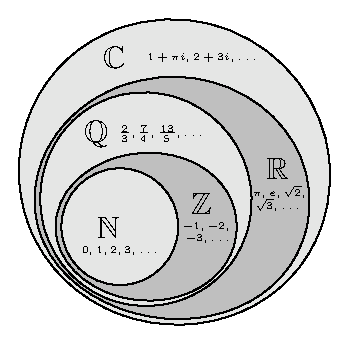
\includegraphics[scale=1]{NumberNotation.eps}
\end{center}
\end{example}

\pagenumbering{arabic} 
\setcounter{page}{1}


\part{Integration}
\begin{comment}

\chapter{How to Find an Antiderivative }

The Fundamental Theorem of Calculus says that an integral (defined as the area under a curve) can be easily evaluated \integ{via antiderivative}.  However, it turns out to be very difficult and sometimes impossible to find an antiderivative!  In this chapter, we give several commonly used methods for antidifferentiation.

\begin{exercise}{What is an Antiderivative Again? \Coffeecup }
\begin{itemize}
\item Complete the \antider{definition} of antiderivative.  That is, if $f(x)$ is a function, then we say $F(x)$ is an antiderivative of $f(x)$ if and only if... 
    \solushun{$$F'(x)=f(x)$$}{.2in}

\item How do you use antiderivatives \antider{to evaluate definite integrals}?  Describe in a short sentence below. 
    \solushun{After finding the antiderivative, you evaluate it at the end and the start of the range over which you want the definite integral, then subtract the latter from the former. That is, $$\int_a^b f(x) \dif x = F(b)-F(a)$$}{.2in}

\item Once you found an antiderivative, what could you do to check that it is correct? (Besides just computing it again!)
    \solushun{Take the derivative of the antiderivative and make sure you get the original function back.\\}
\AnswerKeyEntry{Saying that $F$ is an antiderivative of $f$ is equivalent to saying the derivative of $F$ is $f$.  That is, $F'(x)=f(x)$.  The Fundamental Theorem of Calculus states that after antidifferentiating the integrand, one can plug the bounds into the antiderivative and take their difference in order to calculate the integral.  Because $F'(x)=f(x)$ by the definition of an antiderivative, a good way to check that your antiderivative $F$ is correct is to take its derivative $F'$. You should get the original function, $f$.}
\end{itemize}
\end{exercise}

\section{The Method of \integ{$u$-Substitution}}
\subsection{Undoing the Chain Rule}\label{undo}
The technique of \antider{$u$-substitution} (affectionately known as ``$u$-sub" from here on) can be seen as the reverse of the chain rule for antiderivatives.

\begin{exercise}{What Was the Chain Rule Again? \Coffeecup }
\begin{itemize}
\item First, write down the chain rule. $$\left(f\left(g(x)\right)\right)'= \hspace{2in} $$ 
\solushun{$$\left(f\left(g(x)\right)\right)'= f'(g(x)) \cdot g'(x)$$}{.1in}

\item Take the antiderivative of both sides of that equation.  $$\int \hspace{1in} \dif x= f\left(g(x)\right)+C \hspace{1in} $$
\solushun{$$\int f'(g(x)) \cdot g'(x) \dif x = \int \left(f\left(g(x)\right)\right)' \dif x= f\left(g(x)\right)+C \hspace{1in} $$}{.1in}
\AnswerKeyEntry{$ \intop f'(g(x)) \cdot g'(x) \dif x = \intop \left(f\left(g(x)\right)\right)' \dif x= f\left(g(x)\right)+C$}
\end{itemize}
\end{exercise}
%
In practice, we often make the substitution $u=g(x)$ to condense the notation.  This will take a nastier integral with respect to $x$ and replace it by a hopefully friendlier integral with respect to $u$.  This process of transforming from $x$ to $u$ involves the following three steps: 
%
\begin{enumerate}
\item {\bf Choose $u$:} Pick $u$ to be equal to some expression involving $x$. Frequently, it is helpful to pick $u$ to be some ``inner function'' in a composition of functions that appears in the integrand.  However, there is a \emph{lot} of freedom regarding what substitution you make.  Some choices of $u$ will be helpful, and others will not be!  It is important to be brave and just try some.
\item {\bf Differentiate $u$:} Once you have a formula for $u$, differentiate with respect to $x$ to get a formula for $\frac{\dif u}{\dif x}$.  This will tell us what the conversion factor is between $x$ units and $u$ units.
\item {\bf Solve for $\dif x$:} Use your derivative to solve for $\dif x$.  Substitute that expression for the $\dif x$ in the integral to replace it with $\dif u$.
\end{enumerate}

For the sake of having this process in a nice little formula box, here is the above paragraph rewritten concisely and precisely.
\FormulaBox{$u$-Substitution}{\begin{tabular}{c}
		$\int f'\left(g(x)\right)g'(x)\dif x=\int f'(u) \dif u=f(u)+C=f\left(g(x)\right)+C$
	\end{tabular}}

\begin{example}{An Example of Integration via $u$-sub}\label{sup} To evaluate $ \int x \cos\left( x^2\right) \dif x$, we identify $u=x^2$ as a plausible choice based on our recollection of chain rule.  This gives the following change of variables:
\FormulaBox{Three Steps of $u$-Substitution}{\begin{tabular}{c|c|c}
		Choice of $u$ & Differentiate $u$ & Solve for $\dif x$ \\ \hline
		
		$u=x^2$ & $ \frac{\dif u}{\dif x}=2x$ & $\dif x=\frac{1}{2x}\dif u$
	\end{tabular}}

We now replace $x^2$ by $u$ and replace $\dif x$ by $\frac{1}{2x}\dif u$ in our integral.
$$ \int x \cos\left( x^2\right) \dif x = \int x\cdot \cos(u) \frac{1}{2x}\dif u =\frac{1}{2}\int \cos(u) \dif u=\frac{1}{2}\sin(u)+C=\frac{1}{2}\sin\left(x^2\right)+C$$

\end{example}

\begin{exercise}{Checking Our Work \Coffeecup }
As a follow up to the previous example, differentiate the answer to verify that you end up with the original integrand!

$$\frac{\dif}{\dif x}\left(\frac{1}{2}\sin\left(x^2\right)+C\right)=\hspace{4in}$$
\solushun{$$\frac{\dif}{\dif x}\left(\frac{1}{2}\sin\left(x^2\right)+C\right)=\frac{1}{2}\cdot\frac{\dif}{\dif x}\sin\left(x^2\right)+\frac{\dif}{\dif x}C=\frac{1}{2}\cos\left(x^2\right)\cdot 2x+0=x\cos\left(x^2\right) $$}{.1in}

\end{exercise}

\begin{example}{A Trickier $u$-sub}  Suppose we wish to evaluate the following integral:  $$ \int \frac{\sqrt[3]{x}}{\sqrt[3]{x}+1}\dif x$$ One possible approach is to let $u$ be the denominator.  The denominator can be thought of as the ``inner function'' inside a reciprocal function and thus often makes a good choice for $u$.
\FormulaBox{Three Steps of $u$-Substitution}{\begin{tabular}{c|c|c}
		Choice of $u$ & Differentiate $u$ & Solve for $\dif x$ \\ \hline
		
		$u=\sqrt[3]{x}+1$ & $ \frac{\dif u}{\dif x}=\frac{1}{3}x^{-2/3}$ & $\dif x=3x^{2/3}\dif u$
	\end{tabular}}

We now perform the substitutions on the denominator and the $\dif x$.

$$ \int \frac{\sqrt[3]{x}}{\sqrt[3]{x}+1}\dif x= \int \frac{\sqrt[3]{x}}{u}3x^{2/3}\dif u = 3 \int \frac{x}{u}\dif u  $$

At the moment, it seems like things are going very poorly!  We hoped that $x$ in the numerator would nicely cancel out, like it did back in the more civilized age of Exercise \ref{undo}.\ref{sup}.  To fix this, we solve for $x$ in the equation $u=\sqrt[3]{x}+1$ to obtain $x=\left(u-1\right)^3$.  We now substitute that expression for $x$ in the integral.

\begin{align*}
3 \int \frac{x}{u}\dif u & = 3 \int \frac{\left(u-1\right)^3}{u}\dif u \\
& = 3 \int \frac{u^3-3u^2+3u-1}{u}\dif u \\
& = 3 \int u^2-3u+3-\frac{1}{u} \dif u \\
& = u^3-\frac{9}{2}u^2+9u-3\ln|u| + C \\
& = \left(\sqrt[3]{x}+1\right)^3-\frac{9}{2}\left(\sqrt[3]{x}+1\right)^2+9\left(\sqrt[3]{x}+1\right)-3\ln\left|\sqrt[3]{x}+1\right| + C \\
& = x-\frac{3}{2}\sqrt[3]{x}^2+3\sqrt[3]{x}-3\ln\left|\sqrt[3]{x}+1\right| + C \\
\end{align*}

\end{example}

\begin{exercise}{Missing Constants \Coffeecup }
In the above example, all of the constant terms disappeared on the final step!  Was that ok?  
\vspace{.2in}
\end{exercise}

\begin{exercise}{Practice with $u$-sub \Coffeecup \Coffeecup}
\begin{itemize}
\item Evaluate $\int \frac{6x+3}{x^2+x+8} \dif x$.
\solushun{$$\int \frac{6x+3}{x^2+x+8} \dif x = 3\int \frac{2x+1}{x^2+x+8} \dif x $$
$$\text{Let } u=x^2+x+8 $$
$$\text{Then } \dif u = 2x+1 \dif x $$
$$3\int \frac{\dif u}{u} = 3 \ln u + C = 3 \ln \left(x^2+x+8\right)+C $$}{1.5in}
\item Evaluate $\int \frac{\left(\ln(x)\right)^2}{x} \dif x$.
\solushun{$$\text{Let } u=\ln(x) $$
$$\text{Then } \dif u = \frac{1}{x} \dif x $$
$$\int u^2 \dif u = \frac{u^3}{3}+C= \frac{1}{3}\left(\ln (x)\right)^3+C$$}{1.5in}
\item Evaluate $\int x e^{-x^2} \dif x$.
\solushun{$$\text{Let } u=-x^2 $$
$$\text{Then } \dif u = -2x \dif x \text{ and } \dif x = -\frac{1}{2x}\dif u$$
$$\int x e^{-x^2}\left( -\frac{1}{2x}\dif u\right) = -\frac{1}{2}\int e^u \dif u $$
$$-\frac{1}{2}e^u + C = -\frac{1}{2}e^{-x^2} + C$$}{1.5in}
\item Consider the integral  $$\int  e^{\left(x^2\right)} \dif x$$ Explain in words why the substitution $u=x^2$ will not work in this case.  Where do you get stuck? \solushun{$$\text{Let } u=x^2 $$
$$\text{Then } \dif u = 2x \dif x \text{ and } \dif x = \frac{1}{2x}\dif u$$
$$\int  e^{x^2}\left( \frac{1}{2x}\dif u\right) = \frac{1}{2}\int \frac{e^u}{x} \dif u $$
Here we are stuck because there is no way to cancel $x$ and we can't integrate with two variables.\\}{1.5in}
\AnswerKeyEntry{Use the substitutions $u=x^2+x+8, \ln(x),$ and $-x^2$.  In the last case, the $\dif u$ term has nothing to cancel the $x$ with!}
\end{itemize}
\end{exercise}

\begin{exercise}{Create an Integral! \Coffeecup \Coffeecup \Coffeecup}
 Come up with your own integral that can be evaluated by $u$-sub.  Find a partner and trade!  See if you can evaluate each other's integrals with $u$-sub, or explain to your partner why theirs cannot be evaluated using $u$-sub.

\vspace{2in}
\end{exercise}

\subsection{Change of Coordinates and $u$-Substitution}

The method of $u$-substitution is actually a special case of a more general notion, \emph{change of coordinates}.  This will be studied more thoroughly and in more generality in Calculus 3.  

\begin{example}{How $u$-sub Affects Area}

Suppose we wish to compute the following integral: $$\int_{x=0}^{x=4}\sqrt{2x+1} \dif x $$ 
We interpret this as the \integ{area under the curve} $f(x)=\sqrt{2x+1}$ from $x=0$ to $x=4$ as drawn below.  We apply the substitution $u=2x+1$.
This transforms a region in the $xy$-plane to a region in the $uy$-plane.
\begin{center}
\begin{tabular}{c c}
    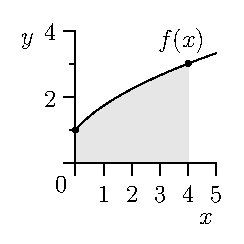
\includegraphics[height=100pt]{ChapterAntidiff/Figures/usubint1.eps}
    %\caption{Graph of $f(x)=\sqrt{2x+1}$} 
	&
    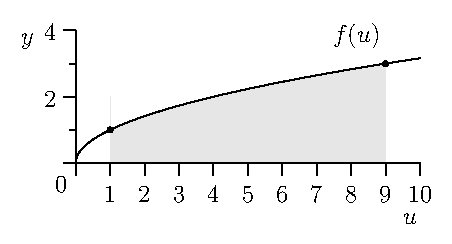
\includegraphics[height=100pt]{ChapterAntidiff/Figures/usubint2.eps}
\end{tabular}
\end{center}

Notice the heights are exactly the same, but the widths have changed by a factor of 2.  Thus to equate the $x$ integral to the $u$ integral, we need to divide the $u$ integral by 2 in order to fix the fact that we doubled all the widths!  In particular, $$\int_{x=0}^{x=4}\sqrt{2x+1} \dif x =\frac{1}{2}\int_{u=1}^{u=9}\sqrt{u} \dif u.  $$
Note that this geometric interpretation corresponds perfectly to what happens in the \integ{Riemann sum} definition of an integral.  For a fixed number of rectangles, the $\Delta x$ in a Riemann sum of the area under $\sqrt{2x+1}$ would be exactly half of the $ \Delta u$ in a corresponding Riemann sum of the area under $\sqrt{u}$.

\end{example}

\begin{exercise}{Relationship between $\Delta x$ and $\Delta u$ \Coffeecup }

\begin{wrapfigure}{r}{0.2\textwidth}
  \centering
  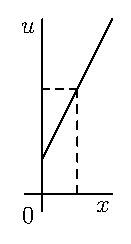
\includegraphics[height=100pt]{ChapterAntidiff/Figures/utox.eps}
  \caption*{Graph of $u=2x+1$, constant derivative 2.}
\end{wrapfigure}
To illustrate the final claim of the example, draw an evenly-spaced four-rectangle Riemann Sum in each of the two shaded regions above.

\begin{itemize}
\item What is your value of $\Delta x$?
\solushun{$$\Delta x = 1$$}{.25in}

\item What is your value of $\Delta u$?
\solushun{$$\Delta u = 2$$}{.25in}

\item Explain where the $u$ bounds of 1 and 9 come from.
\solushun{Since $u=2x+1$, when $x=0$, $u=1$, and when $x=4$, $u=9$. The "$+1$" shifts $u$ 1 unit to the right, just as it would in a graph transformation.\\}{.25in}

\item In the conversion $u=2x+1$, the multiplication by 2 had all the effects described above.  But, why did the ``plus one'' not affect area?  ({\bf Hint:} What would the $u$ bounds have been, and what would the region have looked like, if the ``plus one'' was not there?)
\solushun{Sliding the graph has no effect on its area. If the substitution had been $u=2x$, then the $u$ bounds would have been $0-8$, but the graph would also have started at -1, so the shaded region would be the same in relation to the curve.\\}{.2in}

\item In the figure at right, what aspect of that graph corresponds to the scaling factor between $x$ and $u$?
\solushun{The scaling factor is represented by the slope $\frac{\dif u}{\dif x}$ of the line in the graph at right.\\}{.2in}

\AnswerKeyEntry{To have four intervals in the Riemann sum, $\Delta x$ would be 1 while $\Delta u$ would be 2.  Thus, the width of each rectangle is getting doubled, since to convert between $u$ and $x$ we use the formula $u=2x+1$.  The ``plus one'' merely slides all the rectangles one unit to the right, but it does not stretch their width at all, so it does not affect their area.  Thus, the slope of the graph of $u=2x+1$ is the only thing that mattered regarding our conversion between $x$ and $u$.  That is to say, the quantity $\dif u/ \dif x$ gives us the scaling factor.}
\end{itemize}
\end{exercise}

 The moral to the story is that the scaling factor between $\Delta x$ and $\Delta u$ is in fact the derivative of $u$ with respect to $x$.   In order to translate from $x$ to $u$ in our integral, we must divide by $\frac{du}{dx}$. In this case, that was just the constant 2. 
What is fascinating is that this approach of dividing off by the scaling factor still works, even when the scaling factor is not just a constant.  Hence if we use $u=x^2$, we must divide by $\frac{\dif u }{\dif x}=2x$, as we do in many of the above examples.  It is still a scaling factor, but one that changes depending on the input!  

\begin{exercise}{Looking Graphically at a $u$-sub \Coffeecup \Coffeecup}

% \begin{wrapfigure}{r}{0.2\textwidth}
% 	\centering
%  	%
\begin{asy}
	size(100);  
    import graph;
    
    real f(real x)
    {
        return x^2;
    }
           
    xlimits(0, 3);
	ylimits(0, 4);
    draw(graph(f,0,2,n=400), linewidth(.75bp), arrow=Arrow(HookHead));
    
    draw((0,0)--(1/4,0), linewidth(.5bp), arrow=Arrow(HookHead));
    draw((1/4,1/16)--(1/2,3/16), linewidth(.5bp), arrow=Arrow(HookHead));
    draw((1/2,1/4)--(3/4,1/2), linewidth(.5bp), arrow=Arrow(HookHead));
    draw((3/4,9/16)--(1,15/16), linewidth(.5bp), arrow=Arrow(HookHead));
    draw((1,1)--(5/4,3/2), linewidth(.5bp), arrow=Arrow(HookHead));
    draw((5/4,25/16)--(3/2,35/16), linewidth(.5bp), arrow=Arrow(HookHead));
    draw((3/2,9/4)--(7/4,3), linewidth(.5bp), arrow=Arrow(HookHead));
    
	yaxis("$u$", -.5, 4);
	xaxis("$x$", -.5, 2);
    labelx("$0$",0,1S+1W);
    
\end{asy}
%     \includegraphics[height=100pt]{ChapterAntidiff/utoxsquared.eps}
%  	\caption*{Graph of $u=x^2$, changing derivative of $2x$.}
% \end{wrapfigure}
We now look at a case where the scaling factor depends on $x$.
\begin{itemize}
\item Plot a graph of the function $f(x)=x\sin(x^2)$ on the domain $[0,3]$. (You may use a graphing utility to assist you.)
\solushun{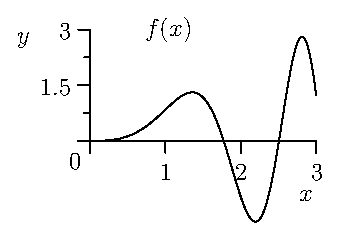
\includegraphics[height=100pt]{ChapterAntidiff/Figures/solxsinx_cropped.eps}\\}{.7in}
\end{itemize}
\begin{minipage}[l]{.75\textwidth}
\begin{itemize}
\item  Plot a graph of the function $h(u)=\sqrt{u}\sin(u)$ on the domain $[0,9]$. (You may use a graphing utility to assist you.)
\solushun{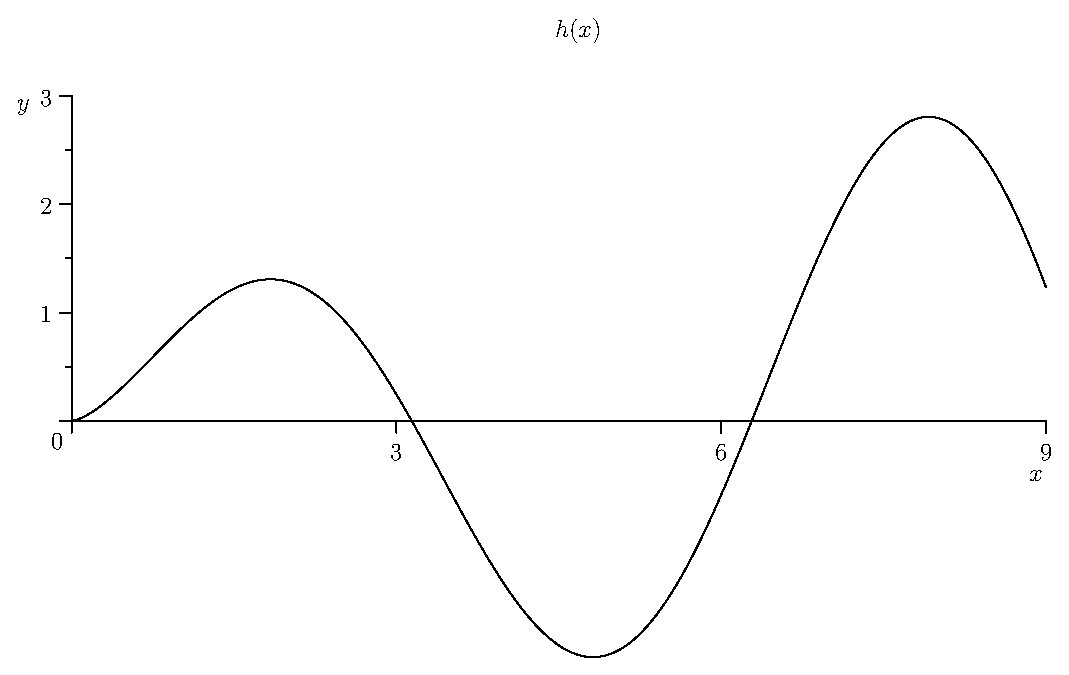
\includegraphics[height=100pt]{ChapterAntidiff/Figures/solusinu_cropped.eps}\\}{.5in}

\item Can you see the horizontal scaling factor change at different points of the graph?  How stretched out does it seem to be at $x=1$?  How stretched out does it seem to be at $x=3$?
\solushun{At $x=1$, the scaling factor is about 1. At $x=3$ the scaling factor is about 9.\\}{.5in}

\item Show algebraically that $u=x^2$ is the substitution that turns that function $f(x)$ into the corresponding function $h(u)$.
\solushun{$$\text{Let } u=x^2 $$
$$\text{Then } x=\sqrt{u}$$
$$\text{Substituting: } x \sin x^2 = \sqrt{u} \sin u$$}{.5in}

\item Evaluate the integral $\int_{x=0}^{x=3}x\sin(x^2)\dif x$.
\solushun{$$\text{Let } u=x^2 \text{, then } \frac{\dif u}{ \dif x} = 2x \text{, and } \dif x = \frac{\dif u}{2x}$$
$$\text{Substituting into the original function:}$$
$$\int_{x=0}^{x=3}x\sin(u)\frac{\dif u}{2x} = \frac{1}{2}\int_{u=0}^{u=9}\sin(u)\dif u = \frac{1}{2} \left[ -\cos (u)\right]_0^9 = \frac{1}{2}\left(-\cos9 + 1\right) \approx 0.955$$}{.5in}

\item In the figure at right, what aspect of that graph corresponds to the scaling factor between $x$ and $u$? 
\solushun{The slope at each point, $\frac{\dif u}{\dif x} = 2x $, is the scaling factor.}{.5in}

\end{itemize} 
\end{minipage}
 \begin{minipage}[r]{0.2\textwidth}
 	\centering
  	%\vspace*{1.75in}
     \includegraphics[height=100pt]{ChapterAntidiff/Figures/utoxsquared.eps} \\
     Graph of $u=x^2$, changing derivative of $2x$.
 \end{minipage}
 
 \AnswerKeyEntry{The definite integral evaluates to roughly 0.95.  The horizontal scaling factor at each $x$-coordinate should correspond to the derivative $\dif u /\dif x$ at each point. }
 
\end{exercise}

\subsection{\trigfunctions{Antiderivatives} of the Six Trig Functions}\label{SixTrigAntiderivatives}

In Calculus I, we found the derivatives of all six trig functions.  List those below.

\begin{exercise}{Recalling the Derivatives of the Six Trig Functions \Coffeecup}
Write the derivative of each of the following trig functions:
\begin{itemize}
\item $\frac{\dif}{\dif x}\left(\sin(x) \right)=$
\item $\frac{\dif}{\dif x}\left(\cos(x) \right)=$
\item $\frac{\dif}{\dif x}\left( \tan(x)\right)=$
\item $\frac{\dif}{\dif x}\left( \cot(x)\right)=$
\item $\frac{\dif}{\dif x}\left( \sec(x)\right)=$
\item $\frac{\dif}{\dif x}\left( \csc(x)\right)=$
\end{itemize}
\solushun{\begin{itemize}
\item $\cos(x)$
\item $-\sin(x)$
\item $\sec^2(x)$
\item $-\csc^2(x)$
\item $\sec(x)\tan(x)$
\item $-\csc(x)\cot(x)$
\end{itemize}}{0in}
\end{exercise}

From these, we easily obtain the antiderivatives of sine and cosine.

\begin{exercise}{Integrals of Sine and Cosine \Coffeecup}
Use the derivatives above to compute the following antiderivatives.
\begin{itemize}
\item $\int \sin(x) \dif x =$
\item $\int \cos(x) \dif x =$
\end{itemize}
\solushun{\begin{itemize}
\item $\int \sin(x) \dif x = -\cos(x) + C$
\item $\int \cos(x) \dif x = \sin(x) + C$
\end{itemize}}{0in}
\end{exercise}

For tangent and cotangent, we need $u$-sub.
\begin{example}{Antiderivative of Tangent}
We compute the \tangent{antiderivative} of tangent by rewriting as $\tan(x)=\frac{\sin(x)}{\cos(x)}$ and then using the substitution $u=\cos(x)$.  Differentiating both sides produces $\dif x = \frac{\dif u}{-\sin(x)}$.  We now apply these substitutions:
\begin{align*}
\int \tan(x) \dif x &= \int \frac{\sin(x)}{\cos(x)}\dif x \\ 
&= \int \frac{\sin(x)}{u}\frac{\dif u}{-\sin(x)} \\
&= -\int \frac{1}{u}\dif u \\
&= -\ln|u|+C \\
&= -\ln|\cos(x)|+C
\end{align*}
\end{example}

The method used to antidifferentiate tangent can be adapted to also antidifferntiate cotangent.
\begin{exercise}{Integral of Cotangent \Coffeecup \Coffeecup}
Find the antiderivative of cotangent.  
$$\int \cot(x) \dif x = \hspace*{3in}$$
\solushun{$$\text{Let } u = \sin(x) \text{, then } \dif x = \frac{\dif u}{\cos x}$$
 \begin{align*}
\int \cot(x) \dif x &= \int \frac{\cos(x)}{\sin(x)}\dif x \\ 
&= \int \frac{\cos(x)}{u}\frac{\dif u}{\cos(x)} \\
&= \int \frac{1}{u}\dif u \\
&= \ln|u|+C \\
&= \ln|\sin(x)|+C
\end{align*}
 }{2in}
\end{exercise}

The \secant{antiderivative} of secant is much trickier!  The process is not intuitive and requires a rabbit out of a hat.
\begin{example}{Integral of Secant} 
Since multiplication by 1 does not change the integrand, we are free to multiply by 1 whenever it is helpful.  Here, it turns out to be helpful to multiply by $\frac{\sec(x)+\tan(x)}{\sec(x)+\tan(x)}$.  This is the rabbit.
\begin{align*}
\int \sec(x)\dif x &=\int \sec(x)\frac{\sec(x)+\tan(x)}{\sec(x)+\tan(x)} \dif x \\
&=\int \frac{\sec^2(x)+\sec(x)\tan(x)}{\sec(x)+\tan(x)} \dif x \\
&=\int \frac{\sec^2(x)+\sec(x)\tan(x)}{u} \frac{1}{\sec(x)\tan(x)+\sec^2(x)}\dif u \\
&=\int \frac{1}{u}\dif u \\
&=\ln|u|+C \\
&=\ln|\sec(x)+\tan(x)|+C
\end{align*}
\end{example}

The above method can be adapted to antidifferentiate cosecant.
\begin{exercise}{Integral of Cosecant \Coffeecup \Coffeecup}
Find the antiderivative of cosecant.  
$$\int \csc(x) \dif x = \hspace*{3in}$$
\solushun{ \begin{align*}
\int \csc(x)\dif x &=\int \csc(x)\frac{\csc(x)+\cot(x)}{\csc(x)+\cot(x)} \dif x \\
&=\int \frac{\csc^2(x)+\csc(x)\cot(x)}{\csc(x)+\cot(x)} \dif x \\
&=\int \frac{\csc^2(x)+\csc(x)\cot(x)}{u} \frac{1}{-\csc(x)\cot(x)-\csc^2(x)}\dif u \\
&=-\int \frac{1}{u}\dif u \\
&=-\ln|u|+C \\
&=-\ln|\csc(x)+\cot(x)|+C
\end{align*}}{2in}
\vspace*{2in}
\end{exercise}


\section{Integration by Parts}\label{ibp}

Integration \integ{by parts} (IBP) is the Product Rule spun around backwards to become a rule for antiderivatives rather than derivatives.  

\begin{exercise}{Reversing the Product Rule \Coffeecup \Coffeecup }
Fill in the blanks in the following construction of \antider{integration by parts}:
\begin{itemize}
\item Recall the Product Rule for derivatives. $$\left( f(x)g(x) \right)'=\hspace{3in} $$
\solushun{$$\left( f(x)g(x) \right)'=f'(x)g(x)+f(x)g'(x)$$}{0in}
\item Take an antiderivative of both sides.
$$ \hspace{2in} = \int \left( f'(x)g(x) \right) \dif x + \int \left( f(x)g'(x) \right) \dif x$$
\solushun{$$ f(x)g(x) = \int \left( f'(x)g(x) \right) \dif x + \int \left( f(x)g'(x) \right) \dif x$$}{0in}
\item Rewrite the equation by subtracting the term $\int \left( f'(x)g(x) \right) \dif x$ from both sides.

$$ = $$
\solushun{$$ f(x)g(x) - \int \left( f'(x)g(x) \right) \dif x = \int \left( f(x)g'(x) \right) \dif x$$}{0in}

\item To condense the notation, it is customary to make the substitutions $u=f(x)$ and $v=g(x)$.  Thus, we say $\frac{\dif u}{\dif x}=f'(x) $ and similarly $\frac{\dif v}{\dif x}=g'(x) $.  Multiply the $\dif x$ to the right-hand side in both of those equations, we obtain

$$\dif u = \hspace{3in} $$ and $$ \dif v = \hspace{3in}  $$

\solushun{$\dif u = f'(x)\dif x $ and $ \dif v = g'(x) \dif x$\\}{0in}

\item Use these substitutions to replace all instances of $x, f, $ and $g$ by $u$ and $v$ and conclude the IBP formula.
\solushun{$$uv-\int v\dif u=\int u\dif v$$\\}{1in}

\end{itemize}
\end{exercise}

Just for sake of having it in its own box, here it is again!
\FormulaBox{Integration by Parts Formula}{\begin{tabular}{c}
		$\int u\dif v=uv-\int v\dif u$
	\end{tabular}}
    
 We typically use this to integrate a product of functions in the case that $u$-substitution does not work.  You can identify one factor of your integrand as $u$, the remaining factor as $\dif v$, and plug into the IBP formula.  There are three main types:

\begin{enumerate}
\item A product with one factor that becomes much simpler upon differentiation
\item A not-quite-a product that we turn into a product
\item An integrand that reappears after applying IBP
\end{enumerate} We illustrate each of these methods with an example.

\subsection{A Product with One Factor That Becomes Much Simpler Upon Differentiation}\label{simpleproduct}  We let $u$ be whichever factor becomes simpler when it is differentiated.  The other factor by default must then be set equal to $\dif v$.  
%\todo[inline]{In a previous example/exercise you did not put a cdot between x and cosine. Below you do.}
%I think this is fine... here I'm specifically drawing attention to the fact that it's a product for sake of IBP
\begin{example}{Integrating a Product}\label{ucosu}
  Suppose we wish to find an antiderivative for the function $x\cdot \cos(x)$.  We can either choose $u=x$ or $u=\cos(x)$.  Since $u=x$ has lovely little constant function 1 as its derivative, whereas $u=\cos(x)$ would produce just another trig function as its derivative, we conclude $u=x$ is the better choice.  

\FormulaBox{Choice of $u$ and $\dif v$}{\begin{tabular}{c|c} 
 $u=x$ &  $v=\sin(x)$ \\ \hline
 $\dif u= \dif x$ & $\dif v=\cos(x)\dif x$ \\ 
\end{tabular}
}

We are now ready to calculate the antiderivative via IBP:
$$\int x\cdot \cos(x) \dif x = \int u \dif v = uv-\int v \dif u = x\cdot \sin(x) - \int \sin(x) \dif x = x\cdot \sin(x) +\cos(x)+C$$

\end{example}

\begin{exercise}{Checking Our Work \Coffeecup}
Take the derivative of our result,  $x \sin(x) +\cos(x)+C$, to verify that it is in fact the correct antiderivative!
\solushun{$$\frac{\dif}{\dif x}\left(x \sin(x) +\cos(x)+C\right) = x\cos(x)+\sin(x)-\sin(x)=x\cos(x)$$}{1.5in}
\end{exercise}

\begin{exercise}{An Integral via both $u$-sub and IBP \Coffeecup \Coffeecup \Coffeecup} Consider the integral $$\int x\sqrt{x+1} \dif x $$
\begin{itemize}
\item Evaluate the integral using the $u$-sub $u=x+1$.
\solushun{Letting $u=x+1$, then $\dif u = \dif x$.
\begin{align*}
\int (u-1)\sqrt{u} \dif x &= \int u^{\frac{3}{2}}-u^\frac{1}{2} \dif u \\
&=\frac{2}{5}u^{\frac{5}{2}}-\frac{2}{3}u^{\frac{3}{2}} \\
&=\frac{2}{5}(x+1)^{\frac{5}{2}}-\frac{2}{3}(x+1)^{\frac{3}{2}} \\
\end{align*}}{2in}
\item Evaluate the integral using IBP, choosing $u=x$ and $\dif v = \sqrt{x+1} \dif x$.
\solushun{Letting $u=x$ and $\dif v = \sqrt{x+1}$, then $\dif u = \dif x$ and $v = \frac{2}{3}(x+1)^\frac{3}{2}$.
\begin{align*}
\int u \dif v &= uv -\int v\dif u \\
&= x\frac{2}{3}(x+1)^\frac{3}{2} -\frac{2}{3}\int (x+1)^\frac{3}{2}\dif x \\
&= \frac{2}{3}x(x+1)^\frac{3}{2} -\frac{2}{3}\left( \frac{5}{2}(x+1)^\frac{5}{2}\right) \\
&= \frac{2}{3}x(x+1)^\frac{3}{2} -\frac{4}{15}(x+1)^\frac{5}{2} \\
\end{align*}}{2in}
\item Your answers will appear very different!  Is one incorrect?  Or are they compatible?
\solushun{
Starting with the first solution from the $u$-sub:
\begin{align*}
\frac{2}{5}(x+1)^{\frac{5}{2}}-\frac{2}{3}(x+1)^{\frac{3}{2}}&=(x+1)^\frac{3}{2}\left(\frac{2}{5}(x+1) -\frac{2}{3}\right)\\
&=(x+1)^\frac{3}{2}\left(\frac{2}{5}x+\frac{2}{5} -\frac{2}{3}\right) \\
&=(x+1)^\frac{3}{2}\left(\frac{2}{5}x -\frac{4} {15}\right) \\
\end{align*}
\\
Starting with the IBP solution:
\begin{align*}
\frac{2}{3}x(x+1)^\frac{3}{2} -\frac{4}{15}(x+1)^\frac{5}{2} &= (x+1)^\frac{3}{2}\left(\frac{2}{3}x -\frac{4}{15}(x+1) \right)\\
&= (x+1)^\frac{3}{2}\left(\frac{2}{3}x -\frac{4}{15}x-\frac{4}{15} \right)\\
&=(x+1)^\frac{3}{2}\left(\frac{2}{5}x -\frac{4} {15}\right) \\
\end{align*}}{2in}
\AnswerKeyEntry{By factoring out the quantity $(x+1)^{3/2}$, both answers can be brought into the form $(x+1)^{3/2}\left(\frac{2}{5}x-\frac{4}{15}\right)+C$.}
\end{itemize}
\end{exercise}

\subsection{A Not-Quite-a Product That We Turn into a Product} Often, an integrand that does not appear to be a product can be rewritten as product in a helpful way.  This often includes {\bf rewriting the integrand as the integrand times one}.  We let $u$ be the entire integrand, leaving $\dif v$ to just be the invisible 1 times $\dif x$.

\begin{example}{Multiplying by 1 in an IBP}
 Suppose we wish to find an antiderivative for the function $\arccos(x)$.  We identify $u=\arccos(x)$ which leaves $\dif v=1\cdot \dif x$.  Thus we make the following declarations:
\FormulaBox{Choice of $u$ and $\dif v$}{\begin{tabular}{c|c} \hline
 $u=\arccos(x)$ &  $v=x$ \\ \hline
 $\dif u=-\frac{1}{\sqrt{1-x^2}}\dif x$ & $\dif v=1\cdot \dif x$ \\ \hline
\end{tabular}}

We are now ready to calculate the antiderivative via IBP:
$$\int \arccos(x)\cdot 1 \cdot \dif x = \int u \dif v = uv-\int v \dif u = x\cdot \arccos(x) - \int x \left( -\frac{1}{\sqrt{1-x^2}} \right) \dif x $$

$$= x\arccos(x) + \int \frac{x}{\sqrt{1-x^2}} \mathtt{dx}=x\arccos(x)-\sqrt{1-x^2}+C $$

\end{example}

\begin{exercise}{Filling in the Details \Coffeecup \Coffeecup}
Notice that the very last step of the above example was in fact a $u$-substitution!  Show the details of how that antiderivative was carried out.

$$\int \frac{x}{\sqrt{1-x^2}}\dif x =\hspace{3in}$$
\solushun{Let $u=1-x^2$. Then $\dif u = -2x \dif x$.
\begin{align}
\int \frac{x}{\sqrt{1-x^2}} \dif x &=-\frac{1}{2}\int \frac{\dif u}{\sqrt{u}} \\
&= -\frac{1}{2}\int u^{-\frac{1}{2}}\dif u \\
&= -\frac{1}{2}\cdot 2 u^{\frac{1}{2}} + C \\
&= -(1-x^2)^{\frac{1}{2}} + C \\
&= -\sqrt{1-x^2} + C \\
\end{align}}{1.5in}
\AnswerKeyEntry{Use the substitution $u=1-x^2$.}
\end{exercise}

\begin{exercise}{The Antiderivative of the Natural Logarithm \Coffeecup \Coffeecup}
Apply the same technique to find an \logarithms{antiderivative} for the function $\ln(x)$.
\solushun{Let $u=\ln(x)$ and $\dif v = 1 \dif x$. Then $\dif u = \frac{1}{x} \dif x$ and $v = x$.
\begin{align}
\int \ln(x) \dif x &= x\ln(x) -\int x \frac{1}{x} \dif x \\
&= x\ln(x)-\int \dif x \\
&= x\ln(x)-x+C \\
\end{align}}{2in}
\AnswerKeyEntry{The antiderivative is $x\ln(x)-x+C$.}
\end{exercise}

\subsection{An Integrand that Reappears After Applying IBP}\label{reappear} Sometimes, we can get the original expression to come back after applying integration by parts one or more times.  Once this occurs, you can {\bf give some name to the integral (we will use $I$)} and solve for it as you would solve any equation in algebra!

\begin{example}{An Integrand that Reappears After IBP}
Suppose we wish to find an antiderivative for the function $e^{2x}\cos(x)$.  Call $I$ the desired antiderivative.  That is:

$$ I=\int e^{2x}\cos(x) \dif x$$ 

We now wish to apply IBP, so we make the following declarations:
\FormulaBox{Choice of $u$ and $\dif v$}{\begin{tabular}{c|c} 
 $u=e^{2x}$ &  $v=\sin(x)$ \\ \hline
 $\dif u=2e^{2x}\dif x$ & $\dif v=\cos(x) \dif x$ \\ 
\end{tabular}
}

We are now ready to calculate the antiderivative via IBP:
\begin{align*} I &= \int u \dif v \\
&= uv-\int v \dif u \\ 
&= e^{2x}\sin(x) - \int \sin(x) \cdot 2e^{2x} \dif x \\
&= e^{2x}\sin(x) -2 \int e^{2x}\sin(x) \dif x \\
\end{align*}

We notice now that the new integral is again a product of functions (and does not appear to be doable via $u$-sub) so we apply IBP once again with the following declarations (using new $u$ and $v$):
\FormulaBox{Choice of $u$ and $\dif v$}{\begin{tabular}{c|c} 
 $u=e^{2x}$ &  $v=-\cos(x)$ \\ \hline
 $\dif u=2e^{2x}\dif x$ & $\dif v=\sin(x) \dif x$ \\ 
\end{tabular}
}

We now proceed with the previous expression, using the new IBP setup and notice that the original integral $I$ reappears:

\begin{align*} I &= e^{2x}\sin(x) -2 \int u \dif v \\
&=e^{2x}\sin(x) -2 \left( uv-\int v \dif u \right) \tag{$\bowtie$} \\
&=e^{2x}\sin(x) -2 \left( e^{2x}(-\cos(x))-\int (-\cos(x))2e^{2x} \dif x \right) \tag{$\bowtie$} \\
&=e^{2x}\sin(x) +2e^{2x}\cos(x)-4\int e^{2x}\cos(x) \dif x \\
&=e^{2x}\sin(x) +2e^{2x}\cos(x)-4I
\end{align*}

At first glimpse this seems troubling; we have reduced the problem we are trying to solve to solving the exact same problem that we are trying to solve!  Yet upon further inspection, it becomes clear that this is in fact an equation involving $I$, and thus we can solve for it!  Proceeding: 

\begin{align*} I&=e^{2x}\sin(x) +2e^{2x}\cos(x)-4I \\
5I&=e^{2x}\sin(x) +2e^{2x}\cos(x) \\
I&=\frac{e^{2x}\sin(x) +2e^{2x}\cos(x)}{5}
\end{align*} and we are done, concluding that $$ \int e^{2x}\cos(x) \dif x=\frac{e^{2x}\sin(x) +2e^{2x}\cos(x)}{5}+C$$

\end{example}

\begin{exercise}{Carefulness \Coffeecup}
In the example above, there are two lines labeled with bowties ($\bowtie$).  Explain briefly in a sentence or two why those giant parentheses are present.  What would go wrong if those parentheses were not there?
\solushun{When IBP is used to evaluate an antiderivative, it is important to distribute the integral's coefficient to both parts of the new expression. If the parentheses weren't there, the coefficients would only be applied to the first expression in each IBP expansion.\\}{1in}
\end{exercise}


\begin{example}{Another Reappearing IBP Integral}\label{AnotherReappearing}
 Suppose we wish to find an antiderivative for the function $\tan(x)\sec^2(x)$.  We identify $\dif v=\sec^2(x) \dif x$ as having a nice clean antiderivative, which leaves $u=\tan(x)$ by default.  Thus we make the following declarations:

\FormulaBox{Choice of $u$ and $\dif v$}{\begin{tabular}{c|c} \hline
 $u=\tan(x)$ &  $v=\tan(x)$ \\ \hline
 $\dif u=\sec^2(x)\dif x$ & $\dif v=\sec^2(x) \dif x$ \\ 
\end{tabular}
}

We are now ready to calculate the antiderivative via IBP:
$$\int \tan(x)\sec^2(x) \dif x = \tan(x)\tan(x) - \int \tan(x) \sec^2(x)\dif x $$

We notice that the original integral has reappeared!  We give it the name $I$ and solve.  The equation becomes $I = \tan^2(x) - I$, which implies that $2I=\tan^2(x)$.  Dividing by two produces the following result:

$$\int \tan(x)\sec^2(x) \dif x =\frac{1}{2}\tan^2(x)+C$$

\end{example}

\begin{exercise}{Alternate Solutions \Coffeecup \Coffeecup }
Find the antiderivative of $\tan(x)\sec^2(x)$ yet again but by two different methods!  In particular, try...
\begin{itemize}
\item ...a $u$-sub with $u=\tan(x)$. 
    \solushun{Let $u=\tan(x)$. Then $\dif u = \sec^2(x)$. Then $$\int \tan(x)\sec^2(x)\dif x = \int u\dif u = \frac{1}{2}u^2+C=\frac{1}{2}\tan^2(x).$$}{1.5in}
\item ...an IBP with $u=\sec(x)$ and $\dif v = \tan(x)\sec(x) \dif x$.
    \solushun{Let $u=\sec(x) and \dif v = \tan(x)\sec(x)$. Then $\dif u = \sec(x)\tan(x)$ and $v=\sec(x)$. Then the integral is
        \begin{align*}
            \int \tan(x)\sec^2(x)\dif x &= \sec^2(x)-\int sec^2(x)\tan(x)\dif x\\
            I &= \sec^2(x)-I\\
            I &= \frac{1}{2}\sec^2(x)+C\\
        \end{align*}
        At this point, note that the arbitrary constant $C$ allows us to shift the antiderivative by whatever we like. If we shift by $-1$, we get
        $$ I = \sec^2(x)-1+C = \frac{1}{2}\tan^2(x)+C.$$
        }{1.5in}
\end{itemize}
Confirm that your answers match the result of Exercise \ref{reappear}.\ref{AnotherReappearing}.
\end{exercise}

\begin{exercise}{A Tricky but Important One: Secant \secant{Cubed} \Coffeecup \Coffeecup \Coffeecup }\label{seccubed}
  Find an antiderivative for the function $\sec^3(x)$.  ({\bf Hint:} Split the cube as $\sec^3(x)=\sec^2(x)\sec(x)$.  Also, the \trigidentities{Pythagorean Identity} $\tan^2(x)=\sec^2(x)-1$ will be useful.)
\solushun{Let $I$ = $\int\sec^3(x) \dif x$ then split the integral:
$$\int \sec^3x \dif x = \int \sec x \sec^2x \dif x$$
Then, let $u=\sec x$ and $\dif v = \sec^2x$. Then $\dif u = \sec x \tan x \dif x$ and $v = \tan x$. 
\begin{align*}
I = \int \sec x \sec^2x \dif x &= \sec x \tan x-\int\tan x \cdot \sec x \tan x \dif x \\
&= \sec x \tan x-\int\tan^2 x \sec x  \dif x \\
&= \sec x \tan x-\int\left(sec^2x-1\right) \sec x  \dif x \\
&= \sec x \tan x-\int \sec^3 x-\sec x  \dif x \\
&= \sec x \tan x-\left(\int \sec^3 x\dif x-\int\sec x  \dif x\right) \\
&= \sec x \tan x-\int \sec^3 x\dif x+\ln|\sec x + \tan x|+C   \\
I &= \sec x \tan x-I+\ln|\sec x + \tan x|+C   \\
2I &= \sec x \tan x+\ln|\sec x + \tan x|+C   \\
I &= \frac{\sec x \tan x+\ln|\sec x + \tan x|}{2} + C
\end{align*}}{4in}
\AnswerKeyEntry{The antiderivative is $\frac{1}{2}\left(\sec(x)\tan(x)+\ln|\sec(x)+\tan(x)|\right)+C$.}
\end{exercise}
\begin{comment}
\subsection{Spot the Error!}
\todo[inline]{I think I'm actually going to put alllll of the STE's at the very end of the section as one big mixed region.}
\todo[inline]{I kind of like that idea. Sort of a review section of mixed practice. Don't tell them what method to use, have spot the errors... Be a good place for old midterm/final problems that you never want to use again.}
In each of the following attempted solutions, there is an error.  Circle where the error occurs and write a short sentence that describes what went wrong.  \begin{enumerate}
\item Find the antiderivative: $ \int \frac{x}{x^2+1} \dif x $
\begin{center}
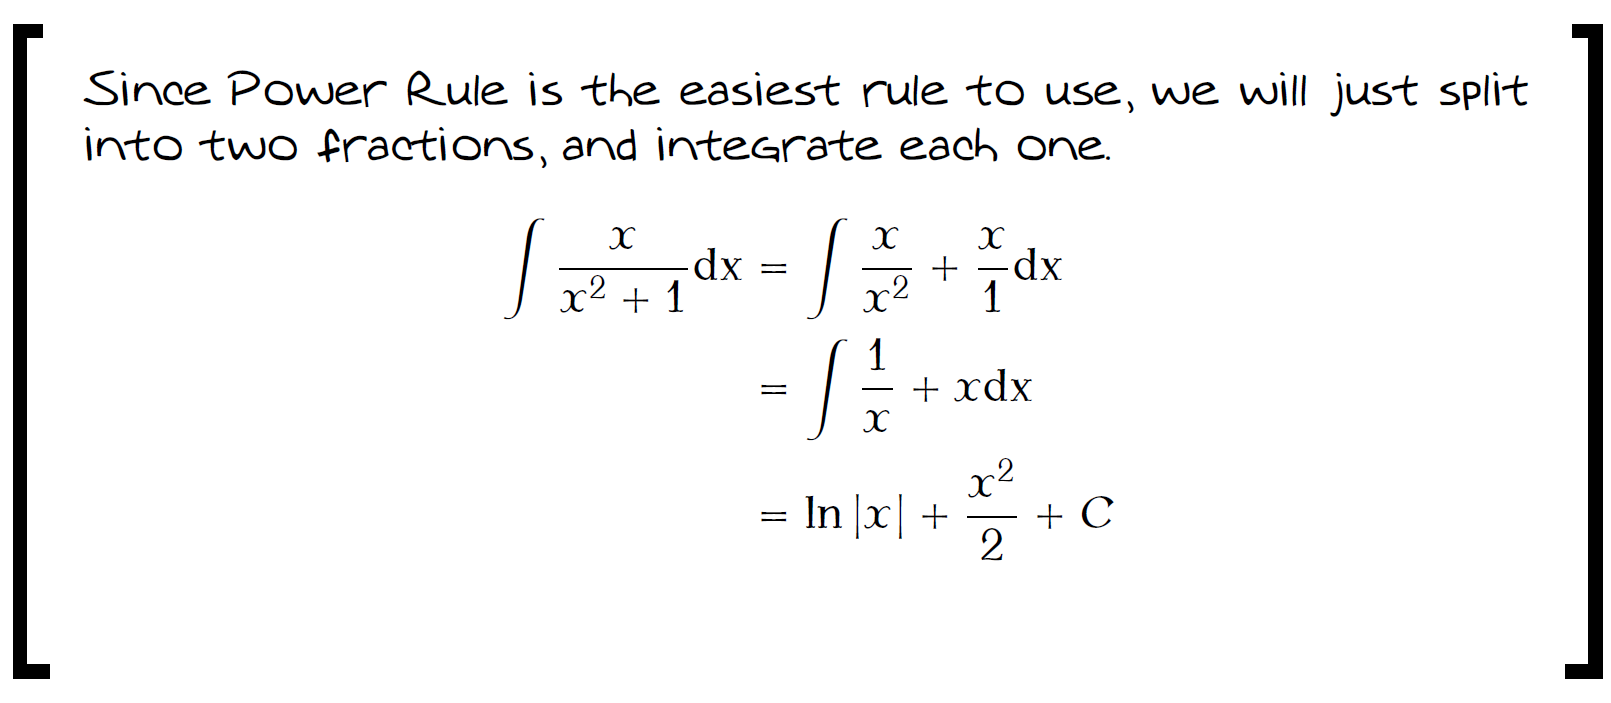
\includegraphics[scale=0.35]{ChapterAntidiff/STEusub.png}
\end{center}

\item Find the antiderivative: $\int x^2\cos(2x) \dif x$
\end{enumerate}

\end{comment}
\section{Mixed Practice with Substitution/IBP}

Sometimes it is not obvious which technique to use in solving a particular problem.  One must often use more than one technique of integration in combination. 

\begin{exercise}{Practice on $u$-sub and/or IBP \Coffeecup \Coffeecup \Coffeecup}
\begin{itemize}
\item Find an antiderivative for the function $\cos(\sqrt{x})$.
\solushun{Start with a $u$-sub. Let $u=\sqrt{x}$. Then $\dif u = \frac{1}{2\sqrt{x}}\dif x$ and $\dif x = 2\sqrt{x}\dif u$
\begin{align*}
\int\cos\sqrt{x}\dif x =\int\cos u\cdot2u\dif u &= 2\int u\cos u\dif u \\
&=2\left(u\sin u + \cos u +C \right) \text{, Example \ref{simpleproduct}.\ref{ucosu}} \\
&=2\sqrt{x}\sin \left(\sqrt{x}\right) + 2\cos\left(\sqrt{x}\right) +C 
\end{align*}}{2in}

\item Evaluate $\int e^{\sqrt{2x}} \dif x$.
\solushun{Start with a $u$-sub. Let $u=\sqrt{2x}$. Then $\dif u = \frac{1}{\sqrt{2x}}\dif x$ and $\dif x = \sqrt{2x}\dif u$
$$\int e^{\sqrt{2x}} \dif x =\int e^{u}\cdot \sqrt{2x} \dif u = \int ue^{u}\dif u $$
Then, proceed with an IBP, using $u=u$, $\dif v=e^u\dif u$, $\dif u=\dif u$, and $v=e^u$.
\begin{align*}
\int ue^{u}\dif u &= ue^u-\int e^{u} \dif u  \\
&=ue^u-e^u +C\\
&=e^u\left(u-1\right) +C\\
&=e^{\sqrt{2x}}\left(\sqrt{2x}-1\right)+C
\end{align*}}{2in}

\item Evaluate $\int \arcsin(5x) \dif x$.
\solushun{Start with a $u$-sub. Let $u=5x$, $\dif u = 5\dif x$:
$$\int\arcsin(5x)\dif x=\frac{1}{5}\int\arcsin(u)\dif u$$
Then, use IBP (we'll use $p,q$ in place of $u,v$ to avoid confusion):
Let $p=\arcsin(u)$ and $\dif q = \dif u$, then $\dif p = \frac{1}{\sqrt{1-u^2}}\dif u$ and $q=u$:

$$\frac{1}{5}\int\arcsin(u)\dif u=\frac{1}{5}\left(u\arcsin(u)-\int\frac{u}{\sqrt{1-u^2}}\dif u\right)$$

Then, we apply another $u$-sub (we will use $v$ to avoid confusion), with $v=1-u^2$ and $\dif v = -2\dif u$, so that $\dif u = -\frac{\dif v}{2u}$

\begin{align*}
\frac{1}{5}\left(u\arcsin(u)-\int\frac{u}{\sqrt{1-u^2}}\dif u\right)&= \frac{1}{5}\left(u\arcsin(u)-\int\frac{u}{\sqrt{v}}\cdot-\frac{\dif v}{2u}\right)\\
&=\frac{1}{5}\left(u\arcsin(u)+\frac{1}{2}\int v^{-\frac{1}{2}}\dif v\right)
\end{align*}

Proceeding:
\begin{align*}
\frac{1}{5}\left(u\arcsin(u)+\frac{1}{2}\int v^{-\frac{1}{2}}\dif v\right) &=\frac{1}{5}\left(u\arcsin(u)+\frac{1}{2}\cdot 2v^{\frac{1}{2}}+C\right)\\
&=\frac{1}{5}\left(u\arcsin(u)+v^{\frac{1}{2}}+C\right)
\end{align*}

Now we back substitute:

\begin{align*}
\frac{1}{5}\left(u\arcsin(u)+v^{\frac{1}{2}}+C\right)&=\frac{1}{5}\left(u\arcsin(u)+\sqrt{1-u^2}+C\right)\\
&=\frac{1}{5}\left(5x\arcsin(5x)+\sqrt{1-(5x)^2}+C\right)\\
&=x\arcsin(5x)+\frac{1}{5}\sqrt{1-(5x)^2}+C
\end{align*}}{2in}

\item Evaluate $\int e^{2x}\sin(2x) \dif x$.
\solushun{$u$-sub: $u=2x$, $\dif u = 5\dif x$:
$$\int e^{2x}\sin(2x)\dif x=\frac{1}{2}\int e^u\sin(u)\dif u$$
IBP with $p=\sin(u)$ and $\dif q = e^u\dif u$, then $\dif p = \cos(u)\dif u$ and $q=e^u$:

$$\frac{1}{2}\int e^u\sin(u)\dif u=\frac{1}{2}\left(e^u\sin(u)-\int e^u\cos(u)\dif u\right)\hspace{.5in}\left(\bowtie\right)$$

Apply a second IBP with $p=\cos(u)$ and $\dif q = e^u\dif u$, then $\dif p = -\sin(u)\dif u$ and $q=e^u$

$$\frac{1}{2}\left(e^u\sin(u)-\int e^u\cos(u)\dif u\right)=\frac{1}{2}\left(e^u\sin(u)-\left(e^u\cos(u)+\int e^u\sin(u)\dif u\right)\right)$$

Notice that $\int e^u\sin(u)\dif u$ is the LHS from $\bowtie$. So we can set $\int e^u\sin(u)\dif u=I$ and equate the last step with $\bowtie$.

\begin{align*}
\frac{1}{2}\int e^u\sin(u)\dif u=\frac{1}{2}I&=\frac{1}{2}\left(e^u\sin(u)-\left(e^u\cos(u)+I\right)\right)\\
\frac{1}{2}I&=\frac{1}{2}e^u\sin(u)-\frac{1}{2}e^u\cos(u)-\frac{1}{2}I\\
I&=\frac{1}{2}e^u\sin(u)-\frac{1}{2}e^u\cos(u)\\
\int e^u\sin(u)\dif u&=\frac{1}{2}e^u\sin(u)-\frac{1}{2}e^u\cos(u)+C\\
2\int e^{2x}\sin(2x)\dif u&=\frac{1}{2}e^{2x}\left(\sin(2x)-\cos(2x)\right)+C \text{, Remember $\dif u = 2\dif x$}\\
\int e^{2x}\sin(2x)\dif 2x&=\frac{1}{4}e^{2x}\left(\sin(2x)-\cos(2x)\right)+C
\end{align*}}{2in}

\end{itemize}
\AnswerKeyEntry{Use the substitution $u=\sqrt{x}$ to transform the first integral into $\intop 2u\cos(u) \dif u$.}
\end{exercise}

\begin{exercise}{Who is $u$ vs Who is $\dif v$? \Coffeecup \Coffeecup}

Suppose we wish to find an antiderivative for the function $x^{2.5}\ln(x)$.  There are two natural choices for $u$.  We can let $u=x^{2.5}$ and $\dif v=\ln(x)\dif x$, or we can let can let $u=\ln(x)$ and $\dif v=x^{2.5}\dif x$.

\begin{itemize}
\item Apply just the first step of IBP with $u=x^{2.5}$ and $\dif v=\ln(x)\dif x$.

$$\int x^{2.5}\ln(x) \dif x = \hspace{3in}$$
\solushun{$$\int x^{2.5}\ln(x) \dif x = x^{2.5}(x\ln(x)-x)-\int \left(x\ln(x)-x\right)\left(2.5x^{1.5}\right)\dif x$$}{0in}

\item Apply just the first step of IBP with $u=\ln(x)$ and $\dif v=x^{2.5}\dif x$.

$$\int x^{2.5}\ln(x) \dif x = \hspace{3in}$$
\solushun{$$\int x^{2.5}\ln(x) \dif x = \frac{x^{3.5}}{3.5}\ln(x)-\frac{1}{3.5}\int x^{2.5}\dif x$$}{0in}

\item Write a short explanation regarding which choice of $u$ will be easier to use to evaluate the integral and why.
\solushun{Choosing $u=\ln(x)$ will make the logarithm disappear upon differentiation, so all we have to evaluate is the integral of a power of $x$.  The opposite choice will not clean up the log.}{1in}

\AnswerKeyEntry{Choosing $u=\ln(x)$ will make the logarithm disappear upon differentiation.  The opposite choice will not clean up the log.}
\item Carry out the integral using whichever choice you decided was easier.

$$\int x^{2.5}\ln(x) \dif x = \hspace{3in}$$
\solushun{$$\frac{x^{3.5}}{3.5}\ln(x)-\frac{1}{3.5}\int x^{2.5}\dif x = \frac{x^{3.5}}{3.5}\ln(x)-\frac{1}{3.5}\cdot\frac{1}{3.5} x^{3.5}=\frac{x^{3.5}}{3.5}\left(\ln(x)-\frac{1}{3.5}\right)+C$$}{1in}

\item Differentiate your answer to check that your antiderivative is correct.
\solushun{
\begin{align*}
\frac{\dif}{\dif x}\left(\frac{x^{3.5}}{3.5}\left(\ln(x)-\frac{1}{3.5}\right)+C \right)&= x^{2.5}\left(\ln(x)-\frac{1}{3.5}\right)+\frac{x^{3.5}}{3.5}\left(\frac{1}{x}\right)\\
&=x^{2.5}\ln(x)-\frac{x^{2.5}}{3.5}+\frac{x^{2.5}}{3.5}\\
&=x^{2.5}\ln(x)
\end{align*}
}{1in}

\end{itemize}
\end{exercise}



\section{Integrating Products of Powers of Sine and Cosine}

In this section, we give an algorithm to find an \sine{\cosine{antiderivative}} of the form $$\int \sin^n(x)\cos^m(x) \dif x$$
for $n,m\in \mathbb{N}$.

\begin{exercise}{Knowledge is Power \Coffeecup}
There are two exponents in the integrand above. 
\begin{itemize}
\item What symbol above is the exponent of sine?  
\item What symbol above is the exponent of cosine?  
\end{itemize}
\end{exercise}

Note that some \antider{sine-cosine} integrals can be done by techniques you have already learned.  For example, $n$ or $m$ is equal to 1, ordinary $u$-substitution will work just fine!

\begin{exercise}{$u$-sub with Sines and Cosines \Coffeecup \Coffeecup}
Evaluate the following integral using the substitution $u=\sin(x)$:
$$\int \sin^2(x)\cos(x)\dif x $$
\solushun{Let $u=\sin(x)$, $\dif u = \cos(x)$. Then:
\begin{align*}
\int \sin^2(x)\cos(x)\dif x &= \int u^2\dif u\\
&=\frac{1}{3}u^3+C\\
&=\frac{1}{3}\sin^3(x)+C
\end{align*}}{2in}
\AnswerKeyEntry{The antiderivative is $\frac{1}{3}\sin^3(x)+C$.}
\end{exercise}

There are two types of integrals containing \integ{powers of sine and cosine}. The first type is the case where we have at least one odd exponent; the second type is where both exponents are even.  We show an overview of how to handle each case in the following awesome flow chart:

 

%\begin{figure}
	%\centering
	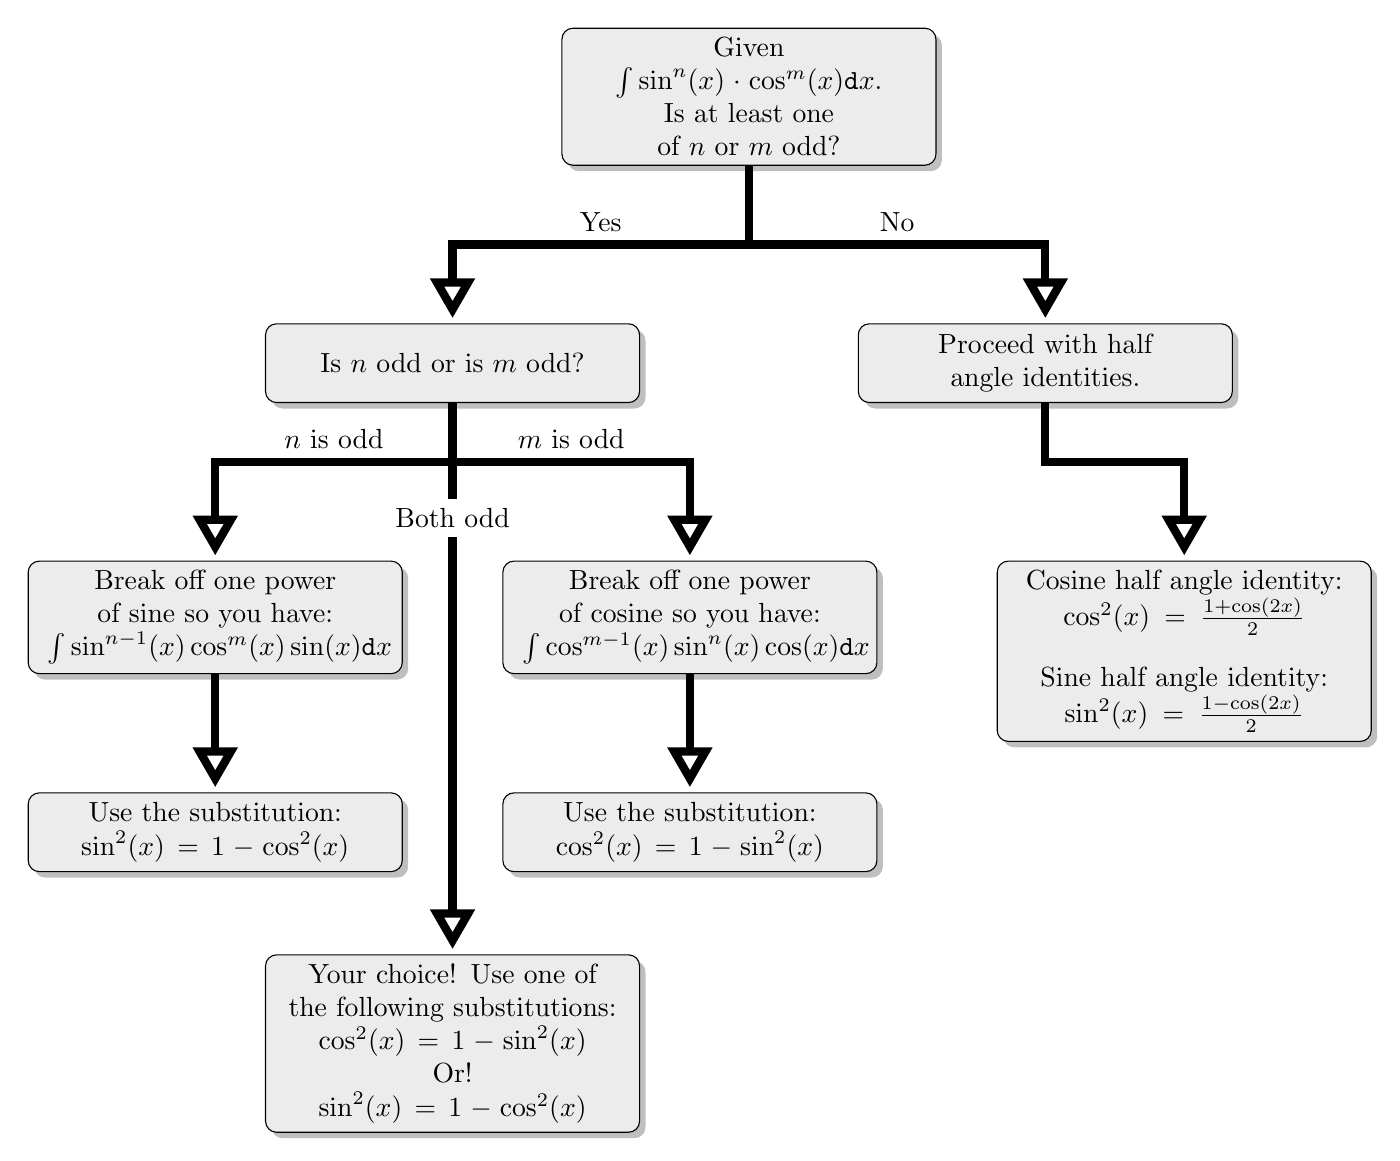
\begin{tikzpicture}[
      >=latex',
      auto
    ]
    
    \tikzstyle{box} = [rectangle, rounded corners, minimum width=4.75cm, minimum height=1cm, text centered, text width=4.25cm, draw=black, fill=gray!15, drop shadow]
    
    \tikzstyle{arrow} = [thick,>=stealth,arrowhead=5mm,->]
    
    \node [box] (given) {
    	Given\\ $\int \sin^n (x) \cdot \cos^m (x) \mathtt{d}x$. \\
        Is at least one of $n$ or $m$ odd?
        };
	\node [box]  (nmOdd) [node distance=2cm and -1cm,below left=of given] {Is $n$ odd or is $m$ odd?};
    \node [box]  (nOdd) [node distance=2cm and -1.75cm,below left=of nmOdd] {Break off one power of sine so you have: \\ 
    $\int \sin^{n-1}(x)\cos^m(x)\sin(x)\mathtt{d}x $ \\};
    \node [box]  (bothOdd) [node distance=7cm,below=of nmOdd] {Your choice! Use one of the following substitutions:
    $\cos^2(x)=1-\sin^2(x)$\\
    Or! \\
    $\sin^2(x)=1-\cos^2(x)$
    };
    
    \node [box]  (nOddSub) [node distance=1.5cm,below=of nOdd] {Use the substitution: \\
    $\sin^2(x)=1-\cos^2(x)$};
    \node [box]  (mOdd) [node distance=2cm and -1.75cm,below right=of nmOdd] {Break off one power of cosine so you have: \\ 
    $\int \cos^{m-1}(x)\sin^n(x)\cos(x)\mathtt{d}x $ \\};
    \node [box]  (mOddSub) [node distance=1.5cm,below=of mOdd] {Use the substitution: \\
    $\cos^2(x)=1-\sin^2(x)$};
    
    \node [box] (nmEven) [node distance=2cm and -1cm,below right=of given] {Proceed with half angle identities.};
    \node [box] (nmEven2) [node distance=2cm and -3cm,below right=of nmEven] {
    Cosine half angle identity: \\
    $\cos^2(x)=\frac{1+\cos(2x)}{2} $ \\
    \vspace{10pt}
    Sine half angle identity: \\
    $ \sin^2(x)=\frac{1-\cos(2x)}{2}$};
    
    
    
    \draw [->, >=open triangle 60, ultra thick,line width= 3pt, shorten >=2pt] (given) -- ($(given.south)+(0,-1)$) -| (nmOdd) node[above,pos=0.25] {Yes} ;
    \draw [->, >=open triangle 60, ultra thick,line width= 3pt, shorten >=2pt] (given) -- ($(given.south)+(0,-1)$) -| (nmEven) node[above,pos=0.25] {No} ;
    
    \draw [->, >=open triangle 60, ultra thick,line width= 3pt, shorten >=2pt] (nmOdd) -- ($(nmOdd.south)+(0,-.75)$) -| (nOdd) node[above,pos=0.25] {$n$ is odd} ;
    \draw [->, >=open triangle 60, ultra thick,line width= 3pt, shorten >=2pt] (nmOdd) -- ($(nmOdd.south)+(0,-.75)$) -| (mOdd) node[above,pos=0.25] {$m$ is odd} ;
    \draw [->, >=open triangle 60, ultra thick,line width= 3pt, shorten >=2pt] (nmOdd) -- (bothOdd) node[above, fill=white, pos=0.25] {Both odd} ;
    
    \draw [->, >=open triangle 60, ultra thick,line width= 3pt, shorten >=2pt] (nOdd) -- (nOddSub) ;
    \draw [->, >=open triangle 60, ultra thick,line width= 3pt, shorten >=2pt] (mOdd) -- (mOddSub) ;
    
    
    \draw [->, >=open triangle 60, ultra thick,line width= 3pt, shorten >=2pt] (nmEven) -- ($(nmEven.south)+(0,-.75)$) -| (nmEven2) ;
	
	\end{tikzpicture}
%\end{figure}

\subsection{At Least One Odd Power}\label{OneOdd}
Recall the Pythagorean identity for sine and cosine (written in two useful forms here): 
\FormulaBox{Pythagorean Theorem Slightly Rewritten}{\begin{tabular}{c|c} \hline
 $   \cos^2(x)=1-\sin^2(x) $ &  $   \sin^2(x)=1-\cos^2(x) $ \\ \hline
\end{tabular}
}

If at least one exponent is odd, we pull one of those functions out for the ``$\dif u$" and perform $u$-sub.  We then use the Pythagorean trig identity to rewrite sine and cosine in terms of each other as needed.  

\begin{example}{Odd Power Case}\label{OddMatters}
 Here we compute the integral $$\int \sin^7(x) \cos^2(x) \dif x$$.  In this case, we proceed using the substitution $u=\cos(x)$, so $\dif x=\frac{1}{-\sin(x)}\dif u$.
 
\begin{align*} \int \sin^7(x) \cos^2(x) \dif x &=\int \sin^6(x) \cos^2(x) \sin(x) \dif x \\
&= \int \left(\sin^2(x)\right)^3 \cos^2(x) \sin(x) \frac{1}{-\sin(x)}\dif u \\
&= \int \left(1-\cos^2(x)\right)^3 \cos^2(x) (-1) \dif u \\
&= -\int \left(1-u^2\right)^3 u^2 \dif u \\
&= -\int \left(1-3u^2+3u^4-u^6\right) u^2 \dif u \\
&= -\int \left(u^2-3u^4+3u^6-u^8\right) \dif u \\
&= -\left(\frac{1}{3}u^3-\frac{3}{5}u^5+\frac{3}{7}u^7-\frac{1}{9}u^9\right)+C \\
&= -\frac{1}{3}\cos^3(x)+\frac{3}{5}\cos^5(x)-\frac{3}{7}\cos^7(x)+\frac{1}{9}\cos^9(x)+C \\
\end{align*}

\end{example}

\begin{exercise}{Why Odd Mattered \Coffeecup}

In Example \ref{OneOdd}.\ref{OddMatters}, the exponent of sine (in this case, the number 7) being odd really mattered.  If that 7 were replaced by an even number instead, why would this approach have failed?  Answer in a few short sentences below.
\solushun{If the exponent of sine had been even, then we couldn't have used the Pythagorean identity to express it in terms of cosine, and still had an extra sine to use with the $u$-sub, which would have prevented us from expressing all the parts in terms of a single expression.\\}{1in}
\AnswerKeyEntry{Since seven is odd, when we pulled out one factor of sine, we ended up with the sixth power of sine remaining.  Since six is even, we were able to express it as a power of a perfect square of sine, which in turn let us rewrite as cosines using the Pythagorean identity.}
\end{exercise}

\begin{exercise}{Try a Few with Odd Exponents \Coffeecup \Coffeecup}

\begin{itemize}
\item Find an antiderivative for the function $\sin^5(x) \cos^2(x)$.
\solushun{\begin{align*}
\int \sin^5(x) \cos^2(x)\dif x &= \int \sin^4(x) \cos^2(x)\sin(x)\dif x\\
&= \int \left(\sin^2(x)\right)^2 \cos^2(x)\sin(x)\dif x\\
&= \int \left(1-\cos^2(x)\right)^2 \cos^2(x)\sin(x)\dif x
\end{align*}
Let $u=\cos(x)$ so $\dif u = -\sin(x)$ and $\dif x = \frac{1}{-\sin(x)}\dif u$
\begin{align*}
\int \left(1-\cos^2(x)\right)^2 \cos^2(x)\sin(x)\dif x&=\int \left(1-u^2\right)^2 u^2\sin(x)\frac{1}{-\sin(x)}\dif u\\
&=\int \left(1-u^2\right)^2 u^2(-1)\dif u\\
&=-\int \left(1-2u^2+u^4\right)u^2\dif u\\
&=-\int u^2-2u^4+u^6\dif u\\
&=-\left(\frac{1}{3}u^3-\frac{2}{5}u^5+\frac{1}{7}u^7+C\right)\\
&=-\frac{1}{3}\cos^3(x)+\frac{2}{5}\cos^5(x)-\frac{1}{7}\cos^7(x)+C
\end{align*}}{2.5in}

\item Evaluate $\int \cos^9(x) \dif x$. ({\bf Hint:} Pascal's Triangle will be extremely helpful!)
\solushun{\begin{align*}
\int \cos^9(x) \dif x&=\int\cos^8(x)\cos(x)\dif x\\
&=\int(1-\sin^2(x))^4\cos(x)\dif x\\
&\text{Let $u=\sin(x)$}\\
&=\int(1-u^2)^4\dif u\\
&=\int1-4u^2+6u^2-4u^6+u^8\dif u\\
&=u-\frac{4}{3}u^3+\frac{6}{3}u^3-\frac{4}{7}u^7+\frac{1}{9}u^9+C\\
&=\sin(x)-\frac{4}{3}\sin^3(x)+\frac{6}{3}\sin^3(x)-\frac{4}{7}\sin^7(x)+\frac{1}{9}\sin^9(x)+C\\
\end{align*}}{2.5in}

\end{itemize}
\AnswerKeyEntry{The first antiderivative is $-\frac{1}{3}\cos^3(x)+\frac{2}{5}\cos^5(x)-\frac{1}{7}\cos^7(x)+C$.  For the second, rewrite as $(1-\sin^2(x))^4\cos(x)$ and proceed by letting $u=\sin(x)$.}
\end{exercise}

\begin{exercise}{Two Different Options \Coffeecup \Coffeecup}
\begin{itemize}

\item  Consider $\int \cos(x)\sin^3(x) \dif x$.
\begin{itemize}
\item  Compute this integral using $u=\cos(x)$.
\solushun{\begin{align*}
\int \cos(x)\sin^3(x)\dif x&=\int\cos(x)\left(1-\cos^2(x)\right)\sin(x)\dif x\\
&=-\int u\left(1-u^2\right)\dif u\\
&=-\int u-u^3\dif u\\
&=-\left(\frac{1}{2}u^2-\frac{1}{4}u^4\right)+C\\
&=-\frac{1}{2}\cos^2(x)+\frac{1}{4}\cos^4(x)+C\\
\end{align*}}{2in}

\item  Compute this integral using $u=\sin(x)$.
\solushun{\begin{align*}
\int \cos(x)\sin^3(x)\dif x&=\int u^3\dif u\\
&=\frac{1}{4}\sin^4(x)+C
\end{align*}}{2in}

\item Your two answers will appear very different!  Show that they are in fact compatible.
\solushun{\begin{align*}
-\frac{1}{2}\cos^2(x)+\frac{1}{4}\cos^4(x)+C&=-\frac{1}{2}(1-\sin^2(x))+\frac{1}{4}(1-\sin^2(x))^2+C\\
&=-\frac{1}{2}+\frac{1}{2}\sin^2(x)+\frac{1}{4}(1-2\sin^2(x)+\sin^4(x))+C\\
&=-\frac{1}{2}+\frac{1}{2}\sin^2(x)+\frac{1}{4}-\frac{1}{2}\sin^2(x)+\frac{1}{4}\sin^4(x)+C\\
&=-\frac{1}{4}+\frac{1}{4}\sin^4(x)+C\\
&\text{$-\frac{1}{4}$ is absorbed into $C$ leaving}\\
&=\frac{1}{4}\sin^4(x)+C\\
\end{align*}}{1in}

\AnswerKeyEntry{Often when trying to show that two antiderivatives are compatible, it is easiest to verify that their difference is a constant. }
\end{itemize}

\item Consider $\int \cos^3(x)\sin^{11}(x) \dif x$.
\begin{itemize}
\item  Can you compute this integral using $u=\cos(x)$?  Explain.
\solushun{Taking $u=\cos(x)$, we can express the integral as $\int\cos^3(x)\left(1-\cos^2(x)\right)^5\cos(x)\dif x=\int u^3\left(1-u^2\right)^5\dif u$\\}{1in}

\item  Can you compute this integral using $u=\sin(x)$?  Explain.
\solushun{We can express the integral as $\left(1-sin^2(x)\right)\sin^11(x)\cos(x)\dif x = \int\left(1-u^2\right)\left(u^{11}\right)\dif x\\$}{1in}

\item Which of the two above substitutions will be easier to use?  Carry out the integration, using the easier of the two.
\solushun{The second option, $u=\sin(x)$ will be easier because it avoids expading a binomial to the 5th power.
Let $u=\sin(x)$
\begin{align*}
\int \cos^3(x)\sin^{11}(x) \dif x &= \left(1-u^2\right)u^{11}\dif u\\
&=\int u^{11}-u^{13}\dif u \\
&=\frac{1}{12}u^{12}-\frac{1}{14}u^{14}+C\\
&=\frac{1}{12}\sin^{12}(x)-\frac{1}{14}\sin^{14}(x)+C
\end{align*}}{2.5in}

\AnswerKeyEntry{The substitution $u=\sin(x)$ is much cleaner since the other will involve having to expand a binomial to the fifth power.  The antiderivative is $\frac{1}{12}\sin^{12}(x)-\frac{1}{14}\sin^{14}(x)+C$.}
\end{itemize}
\end{itemize}

\end{exercise}

\subsection{Both Even Powers}

Recall the \trigidentities{Half-Angle Identities}!
\FormulaBox{Half-Angle Identities}{
\begin{tabular}{c|c} \hline
 $     \cos^2(x)=\frac{1+\cos(2x)}{2}  
   $ &  $    \sin^2(x)=\frac{1-\cos(2x)}{2} $ \\ \hline
\end{tabular}}

If the \halfangle{powers of sine and cosine} are both even, we use the half-angle identities for both sine and cosine.  This can get quite messy, but it works!

\begin{exercise}{Just Cosines without Sine \Coffeecup}
 Consider the following integral: $$\int \cos^6(x)\dif x $$ Here the exponent on cosine is the even number 6.  What is the exponent of sine in that integrand?  Is that an even number? 
 \solushun{The exponent on sine is zero, which is indeed even.  Thus both exponents are even in this case.\\}{.2in}
 \AnswerKeyEntry{The exponent on sine is zero, which is indeed even.  Thus both exponents are even in this case.}
 \end{exercise}
 
\begin{example}{Carrying Out Antidifferentiation with the Half-Angle Identities}
We now show how the half-angle identities help antidifferentiate the sixth power of cosine. 

\begin{align*} \int  \cos^6(x) \dif x &=\int \left(\cos^2(x)\right)^3  \dif x \\
&=\int \left(\frac{1+\cos(2x)}{2}\right)^3  \dif x \\ 
&=\frac{1}{8}\int 1+3\cos(2x)+3\cos^2(2x)+\cos^3(2x)  \dif x \\
&=\frac{1}{8}\left(\int 1\dif x+\int 3\cos(2x)\dif x+\int 3\cos^2(2x)\dif x+\int \cos^3(2x) \dif x\right)
\end{align*}

Notice that we now have four integrals.  The first is easy, the second is a $u$-substitution, and the third is another even power of cosine (where we again use the half-angle identity).  Finally, the fourth is an odd power of cosine, so we can use the technique from Section \ref{OneOdd}.  

\end{example}

\begin{exercise}{Finishing the Example \Coffeecup \Coffeecup}
Carry out each of these processes to compute the four integrals:
\begin{itemize}
\item $\int 1\dif x$
\solushun{$$\int 1\dif x=x+C$$}{.2in}
\item $\int 3\cos(2x)\dif x$
\solushun{
Let $u=2x$. Then,
$$\int3\cos2x\dif x = \frac{3}{2}\int\cos u\dif u =\frac{3}{2}\sin2x+C$$}{1in}
\item $\int 3\cos^2(2x)\dif x$
\solushun{$$\int 3\cos^2(2x)\dif x=3\int\frac{1+\cos4x}{2}\dif x=3\left(\frac{1}{2}x +\frac{1}{8}\sin4x+C\right)=\frac{3}{2}x +\frac{3}{8}\sin4x+C$$}{1.5in}
\item $\int \cos^3(2x) \dif x$
\solushun{Let $u=\sin2x$ and $\dif u = 2\cos2x\dif x$. Then, 
\begin{align*}\int \cos^3(2x) \dif x&=\int \cos2x\left(1-\sin^22x\right)\dif x\\&=\frac{1}{2}\int1-u^2\dif u\\&=\frac{1}{2}u-\frac{1}{6}u^3+C\\&=\frac{1}{2}\sin2x-\frac{1}{6}\sin^32x+C\end{align*}}{1.5in}
\end{itemize}

Add your antiderivatives together and combine like terms to produce your final answer for the integral!  Oh and remember that one-eighth.

$$ \int  \cos^6(x) \dif x = \hspace{4in} $$ 
\solushun{$$
\frac{1}{8}\left(x+\frac{3}{2}\sin2x+\frac{3}{2}x+\frac{3}{8}\sin4x+\frac{1}{2}\sin2x-\frac{1}{6}\sin^32x+C\right)$$ $$=\frac{1}{8}\left(\frac{5}{2}x+2\sin2x+\frac{3}{8}\sin4x-\frac{1}{6}\sin^32x+C\right)$$
$$=\frac{5}{16}x+\frac{1}{4}\sin(2x)-\frac{1}{48}\sin^3(2x)+\frac{3}{64}\sin(4x)+C
$$}{.5in}

\AnswerKeyEntry{When all like terms are combined and the one-eighth is distributed, the result is $\frac{5}{16}x+\frac{1}{4}\sin(2x)-\frac{1}{48}\sin^3(2x)+\frac{3}{64}\sin(4x)+C$.}
\end{exercise}

\begin{exercise}{Checking the Previous Example \Coffeecup \Coffeecup \Coffeecup}
Differentiate your answer and verify you get the original integrand back.
\solushun{$$\frac{\dif}{\dif x}\left(\frac{5}{16}x+\frac{1}{4}\sin(2x)-\frac{1}{48}\sin^3(2x)+\frac{3}{64}\sin(4x)+C\right)$$ Before we differentiate, first bash everything back down to an ``$x$''
in the argument using double angle identities.  This produces

$$\frac{5}{16}x+\frac{1}{2}\sin(x)\cos(x)-\frac{1}{6}\sin^3(x)\cos^3(x)+\frac{3}{16}\sin(x)\cos^3(x)-\frac{3}{16}\sin^3(x)\cos(x)+C$$
Factor out a sine and use the Pythagorean Identity to get everything else in terms of cosine.  This produces $$\frac{5}{16}x+\sin(x)\left(\frac{5}{16}\cos(x)+\frac{5}{24}\cos^3(x)+\frac{1}{6}\cos^5(x)\right)+C$$  
Then we differentiate and obtain $$\frac{5}{16}+\cos(x)\left(\frac{5}{16}\cos(x)+\frac{5}{24}\cos^3(x)+\frac{1}{6}\cos^5(x)\right)-\sin^2(x)\left(\frac{5}{16}+\frac{5}{8}\cos^2(x)+\frac{5}{6}\cos^4(x)\right)$$ to which we apply the Pythagorean Identity $\sin^2(x)=1-\cos^2(x)$ to produce $$\frac{5}{16}+\cos(x)\left(\frac{5}{16}\cos(x)+\frac{5}{24}\cos^3(x)+\frac{1}{6}\cos^5(x)\right)-\left(1-\cos^2(x)\right)\left(\frac{5}{16}+\frac{5}{8}\cos^2(x)+\frac{5}{6}\cos^4(x)\right)$$
This will simplify to $\cos^6(x)$ once you expand and combine like terms.\\}{2in}
 
\AnswerKeyEntry{The antiderivative to $\cos^6(x)$ came out to

$$\frac{5}{16}x+\frac{1}{4}\sin(2x)-\frac{1}{48}\sin^3(2x)+\frac{3}{64}\sin(4x)+C$$ Before we differentiate, first bash everything back down to an ``$x$''
in the argument using double angle identities.  This produces

$$\frac{5}{16}x+\frac{1}{2}\sin(x)\cos(x)-\frac{1}{6}\sin^3(x)\cos^3(x)+\frac{3}{16}\sin(x)\cos^3(x)-\frac{3}{16}\sin^3(x)\cos(x)+C$$
Factor out a sine and use the Pythagorean Identity to get everything else in terms of cosine.  This produces $$\frac{5}{16}x+\sin(x)\left(\frac{5}{16}\cos(x)+\frac{5}{24}\cos^3(x)+\frac{1}{6}\cos^5(x)\right)+C$$  
Then we differentiate and obtain $$\frac{5}{16}+\cos(x)\left(\frac{5}{16}\cos(x)+\frac{5}{24}\cos^3(x)+\frac{1}{6}\cos^5(x)\right)-\sin^2(x)\left(\frac{5}{16}+\frac{5}{8}\cos^2(x)+\frac{5}{6}\cos^4(x)\right)$$ to which we apply the Pythagorean Identity $\sin^2(x)=1-\cos^2(x)$ to produce $$\frac{5}{16}+\cos(x)\left(\frac{5}{16}\cos(x)+\frac{5}{24}\cos^3(x)+\frac{1}{6}\cos^5(x)\right)-\left(1-\cos^2(x)\right)\left(\frac{5}{16}+\frac{5}{8}\cos^2(x)+\frac{5}{6}\cos^4(x)\right)$$
This will simplify to $\cos^6(x)$ once you expand and combine like terms.
}
\end{exercise}

\begin{exercise}{Practice with the Even Case \Coffeecup \Coffeecup}
\begin{itemize}

\item  Find an antiderivative for the function $\sin^2(3x)$.
\solushun{\begin{align*}
\int\sin^2(3x)&=\int\frac{1-\cos(6x)}{2}\dif x\\
&=\int\frac{1}{2}-\frac{1}{2}\cos(6x)\dif x\\
\text{Let $u=6x, \dif u=6\dif x$}\\
&=\frac{1}{2}x-\frac{1}{2}\cdot\frac{1}{6}\int\cos u\dif u\\
&=\frac{1}{2}x-\frac{1}{12}\sin u+C\\
&=\frac{1}{2}x-\frac{1}{12}\sin 6x+C
\end{align*}}{1in}
\item  Find an antiderivative for the function $\sin^4(x)$.  
\solushun{\begin{align*}
\int\sin^4(x)\dif x&=\int\left(\sin^2(x)\right)^2\dif x\\
&=\int\left(\frac{1-\cos(2x)}{2}\right)^2\dif x\\
&=\int\frac{1-2\cos(2x)+cos^2(2x)}{4}\dif x\\
&=\int\frac{1}{4}-\frac{1}{2}\cos(2x)+\frac{1}{4}\cdot\frac{1+\cos(4x)}{2}\dif x \\
&=\int\frac{1}{4}-\frac{1}{2}\cos(2x)+\frac{1}{8}+\frac{1}{8}\cos(4x)\dif x \\
&=\int\frac{3}{8}-\frac{1}{2}\cos(2x)+\frac{1}{8}\cos(4x)\dif x \\
&=\frac{3}{8}x-\frac{1}{4}\sin(2x)+\frac{1}{32}\sin(4x) +C\\
\end{align*}}{2in}

\item  Find an antiderivative for the function $\sin^2(x)\cos^2(x)$.
\solushun{\begin{align*}
\int\sin^2(x)\cos^2(x)\dif x&=\int\sin^2(x)\left(1-\sin^2(x)\right)\dif x \\
&=\int\sin^2(x)-\sin^4(x)\dif x \\
\text{From previous examples: }\\
\int\sin^2(x)\dif x &= \frac{1}{2}x-\frac{1}{2}\sin x+C\\
\int\sin^4(x)\dif x &= \frac{3}{8}x-\frac{1}{4}\sin(2x)+\frac{1}{32}\sin(4x) +C\\
\int\sin^2(x)-\sin^4(x)\dif x &=\frac{1}{2}x-\frac{1}{2}\sin x-\left(\frac{3}{8}x-\frac{1}{4}\sin(2x)+\frac{1}{32}\sin(4x)\right)+C\\
&=\frac{1}{2}x-\frac{1}{2}\sin x-\frac{3}{8}x+\frac{1}{4}\sin(2x)-\frac{1}{32}\sin(4x)+C\\
&=\frac{1}{8}x-\frac{1}{2}\sin x+\frac{1}{4}\sin(2x)-\frac{1}{32}\sin(4x)+C\\
\end{align*}}{2in}

\AnswerKeyEntry{For the first, apply the identity $\sin^2(3x)=\frac{1-\cos(6x)}{2}$ and proceed.  For the second, notice that $\sin^4(x)$ can be rewritten as $\left(\sin^2(x)\right)^2$, after which the half-angle identity can be applied.}
\end{itemize}
\end{exercise}

\section{\trigsub{Trigonometric Substitution}}

Though in theory you could use any trigonometric function, the three commonly used \trigfunctions{\integ{trigonometric substitutions}} are sine, tangent, and secant.  The substitutions are motivated by the Pythagorean Identities from trigonometry.

\begin{exercise}{Recalling the Pythagorean Identities \Coffeecup} 
\begin{itemize}
\item Start with the \trigidentities{Pythagorean Identity} for sine and cosine: $$\cos^2\left(\theta\right)+\sin^2\left(\theta\right)=1 $$
\item Subtract $\sin^2\left(\theta\right) $ from both sides.  Write the resulting equation below.
\solushun{$$\cos^2(\theta)=1-\sin^2(\theta)$$}{.2in}
\item Again, start with the Pythagorean Identity for sine and cosine.  What would we have to divide both sides by in order to get the corresponding identity for tangent and secant (written below)?
$$1+\tan^2\left(\theta\right)=\sec^2\left(\theta\right) $$
\solushun{Divide everything by $\cos^2(\theta)$
$$\frac{\cos^2\left(\theta\right)}{\cos^2\left(\theta\right)}+\frac{\sin^2\left(\theta\right)}{\cos^2\left(\theta\right)}=\frac{1}{\cos^2\left(\theta\right)}$$
$$1+\tan^2\left(\theta\right)=\sec^2\left(\theta\right)$$}{.2in}
\item How would you then obtain the identity below?
$$\sec^2\left(\theta\right)-1=\tan^2\left(\theta\right) $$
\solushun{Subtract $1$ from both sides.\\}{.2in}
\end{itemize}
\end{exercise}

You can take any of the identities above and multiply both sides by $a^2$ (where $a$ represents an arbitrary positive real constant) to produce a more general identity.  This is what results in the commonly used \antider{trigonometric substitutions} for integrals, summarized in the table below.

\FormulaBox{Trigonometric Substitutions}{
\begin{tabular}{c|c|c} \hline 
 If you see... &   ...make the substitution... & ...because...  \\ \hline 
 $a^2-x^2$ &  $  x=a \sin\left(\theta\right) $ & $a^2-a^2\sin^2\left(\theta\right)=a^2\cos^2\left(\theta\right) $ \\
 $a^2+x^2$ &  $  x=a \tan\left(\theta\right) $ & $a^2+a^2\tan^2\left(\theta\right)=a^2\sec^2\left(\theta\right) $ \\
$x^2-a^2$ &  $  x=a \sec\left(\theta\right) $ & $a^2\sec^2\left(\theta\right)-a^2=a^2\tan^2\left(\theta\right) $ \\
\end{tabular}}

\begin{exercise}{Why Only Three Cases? \Coffeecup} In the table above, we have cases for how to clean up expressions of the form $a^2-x^2$, $a^2+x^2$, and $x^2-a^2$.  Why is there not a fourth case for $x^2+a^2$?
\solushun{The case $x^2+a^2$ is equivalent to the case $a^2+x^2$, so we can rearrange the expression and use the substitution $x=a\tan(\theta)$\\}{.2in}
\end{exercise}%
%
\subsection{\sine{Sine Substitution}} When we see an expression of the form $a^2-x^2$ in the integrand, we think of the identity $1-\sin^2(\theta)=\cos^2(\theta)$.  This motivates the following substitution:

\FormulaBox{Sine Substitution}{\begin{tabular}{c}
		$x=a\cdot \sin(\theta)$
	\end{tabular}
}

The next example will require use of the \trigidentities{Double-Angle Identities} for sine and cosine.  We recall these before we dive in!

\begin{exercise}{Recalling the Double-Angle Formulas \Coffeecup}
\begin{itemize}
\item The double-angle formula for sine is $\sin(2\theta)=$
\solushun{$\sin(2\theta)=2\sin(\theta)\cos(\theta)$\\}{0in}
\item The double-angle formula for cosine is $\cos(2\theta)=$
\solushun{$\cos(2\theta)=\cos^2(\theta)-\cos^2(\theta)$\\}{0in}
\item What do you get if you apply the sine double-angle identity to $\sin(4\theta)$?  Specifically, think of $\sin(4\theta)$ as $\sin\left(2\cdot 2\theta \right)$. 
\solushun{$\sin(4\theta)=2\sin(2\theta)\cos(2\theta)$\\}{.2in}\vspace*{.2in}
\end{itemize}
\end{exercise}

We now put our sine substitution to use to evaluate an antiderivative!
\begin{example}{Using a Sine Substitution}
 Suppose we wish to evaluate $$\int \left( 4-x^2 \right)^{3/2} \dif x$$
  
We use the substitution suggested above, specifically $$x=2\cdot \sin(\theta).$$  We then differentiate both sides to find the conversion between the differentials and then multiply both sides by $\dif \theta$: $$ \frac{\dif x}{\dif \theta}=2 \cdot \cos(\theta) $$

We now use the above equations to substitute for $x$ and $\dif x$ in the integral:

\begin{align*} \int \left( 4-x^2 \right)^{3/2} \mathtt{d}x &=\int \left( 4-(2\cdot \sin(\theta))^2 \right)^{3/2} 2\cdot \cos(\theta)\mathtt{d}\theta \\
&=2 \int \left(4-4\cdot \sin^2(\theta)\right)^{3/2}\cos(\theta) \mathtt{d}\theta \\
&=2 \int \left(4\left(1-\sin^2(\theta)\right)\right)^{3/2}\cos(\theta) \mathtt{d}\theta \\
&=2 \int \left(4\left(\cos^2(\theta)\right)\right)^{3/2}\cos(\theta) \mathtt{d}\theta \\
&=2 \int \left(4\right)^{3/2}\left(\cos^2(\theta)\right)^{3/2}\cos(\theta) \mathtt{d}\theta
\\
&=16 \int \cos^3(\theta)\cdot \cos(\theta) \mathtt{d}\theta
\\
&=16 \int \cos^4(\theta) \mathtt{d}\theta
\end{align*}

Recall the previous section where we learned how to antidifferentiate even powers of sine and cosine!  Accordingly, we use the half-angle identities.

\begin{align*} \int \left( 4-x^2 \right)^{3/2} \mathtt{d}x &=16 \int \left(\cos^2(\theta)\right)^2 \mathtt{d}\theta \\
&=16 \int \left(\frac{1+\cos(2\theta)}{2}\right)^2 \mathtt{d}\theta \\
&=16 \int \frac{1+2\cdot \cos(2\theta)+\cos^2(2\theta)}{4} \mathtt{d}\theta \\
&=4 \int 1+2\cdot \cos(2\theta)+\cos^2(2\theta) \mathtt{d}\theta \\
&=4 \int 1+2\cdot \cos(2\theta)+\frac{1+\cos(4\theta)}{2} \mathtt{d}\theta \\
&=4 \int \frac{3}{2}+2\cdot \cos(2\theta)+\frac{1}{2}\cos(4\theta) \mathtt{d}\theta \\
&=4 \left( \frac{3}{2}\theta +\sin(2\theta) +\frac{1}{8}\sin(4\theta) \right)+C \\
&=6\theta +4\cdot \sin(2\theta) +\frac{1}{2}\sin(4\theta)+C
\end{align*}

We have successfully taken the antiderivative!  However, it still remains to unwind the \doubleangle{trigonometric substitution} back in terms of $x$ rather than $\theta$.  Our original substitution argument is $\theta$, whereas currently we have $2\theta $ and $4\theta $ as arguments.  In order to resolve this, we use the sine and cosine double angle formulas and the Pythagorean identity.  Proceeding:
\begin{align*} \int \left( 4-x^2 \right)^{3/2} \mathtt{d}x &=6\theta +4\cdot \sin(2\theta) +\frac{1}{2}\sin(4\theta)+C \\
&=6\theta +4\cdot 2\cdot \sin(\theta)\cos(\theta) + \sin(2\theta)\cos(2\theta)+C \\
&=6\theta +4\cdot 2\cdot \sin(\theta)\cos(\theta) +2\cdot \sin(\theta)\cos(\theta)\left(\cos^2(\theta)-\sin^2(\theta)\right)+C \\
&=6\theta +8\cdot \sin(\theta)\sqrt{1-\sin^2(\theta)} +2\cdot \sin(\theta)\sqrt{1-\sin^2(\theta)}\left(1-2\sin^2(\theta)\right)+C \\
&=6\cdot \arcsin\left(\frac{x}{2}\right)+8\frac{x}{2}\sqrt{1-\frac{x^2}{4}}+2\frac{x}{2}\sqrt{1-\frac{x^2}{4}}\left(1-2\frac{x^2}{4}\right)+C \\
&=6\cdot \arcsin\left(\frac{x}{2}\right)+4x\sqrt{1-\frac{x^2}{4}}+\sqrt{1-\frac{x^2}{4}}\left(x-\frac{x^3}{2}\right)+C
\end{align*}

\end{example}
 \begin{exercise}{Checking Our Work \Coffeecup \Coffeecup \Coffeecup }
Verify the result of the previous example by differentiating! 
\solushun{First apply all the product and chain rules to reach the expression $$\frac{3}{\sqrt{1-\frac{x^2}{4}}}+4\sqrt{1-\frac{x^2}{4}}+\frac{-x^2}{\sqrt{1-\frac{x^2}{4}}}+\sqrt{1-\frac{x^2}{4}}\left(1-\frac{3}{2}x^2\right)+\frac{-x}{4\sqrt{1-\frac{x^2}{4}}}\left(x-\frac{x^3}{2}\right) $$  Put all terms over the common denominator $\sqrt{4-x^2}$ and combine like terms in the numerator.
\begin{align*}
&=\frac{3\cdot2}{\sqrt{4-x^2}}+\frac{2\cdot 4\left(1-\frac{x^2}{4}\right)-2x^2}{\sqrt{4-x^2}}+\frac{4(1-\frac{x^2}{4})\left(1-\frac{3}{2}x^2\right)-x\left(x-\frac{x^3}{2}\right)}{4\sqrt{1-\frac{x^2}{4}}}\\
&=\frac{6}{\sqrt{4-x^2}}+\frac{8-2x^2-2x^2}{\sqrt{4-x^2}}+\frac{4-6x^2-x^2+\frac{3}2{x^4}-x^2+\frac{x^4}{2}}{4\sqrt{1-\frac{x^2}{4}}}\\
&=\frac{6}{\sqrt{4-x^2}}+\frac{8-4x^2}{\sqrt{4-x^2}}+\frac{2-4x^2+{x^4}}{\sqrt{4-x^2}}\\
&=\frac{16-8x^2+x^4}{\sqrt{4-x^2}}\\
&=\frac{\left(4-x^2\right)^2}{\sqrt{4-x^2}}\\
&=\left(4-x^2\right)^\frac{3}{2}
\end{align*}}{3in}
\AnswerKeyEntry{First apply all the product and chain rules to reach the expression $$\frac{3}{\sqrt{1-\frac{x^2}{4}}}+4\sqrt{1-\frac{x^2}{4}}+\frac{-x^2}{\sqrt{1-\frac{x^2}{4}}}+\sqrt{1-\frac{x^2}{4}}\left(1-\frac{3}{2}x^2\right)+\frac{-x}{4\sqrt{1-\frac{x^2}{4}}}\left(x-\frac{x^3}{2}\right) $$  Put all terms over the common denominator $\sqrt{4-x^2}$ and combine like terms in the numerator.  Notice the numerator becomes $\left(4-x^2\right)^2$ and then reduce for the win!}
\end{exercise}
\subsubsection{An Alternate Approach}
In the above example, we made it back from $\theta$ to $x$ by just bashing it to bits with trig identities.  Sometimes a cleaner approach can be to use a little geometry.  Since we had the substitution $x=2\sin(\theta)$, we can divide both sides by 2 to obtain the following:  $$\sin(\theta)=\frac{x}{2}$$ 

Since sine is the ratio of the opposite side to the hypotenuse in a right triangle, we can label the opposite side as $x$ and the hypotenuse as 2. 
\begin{center}
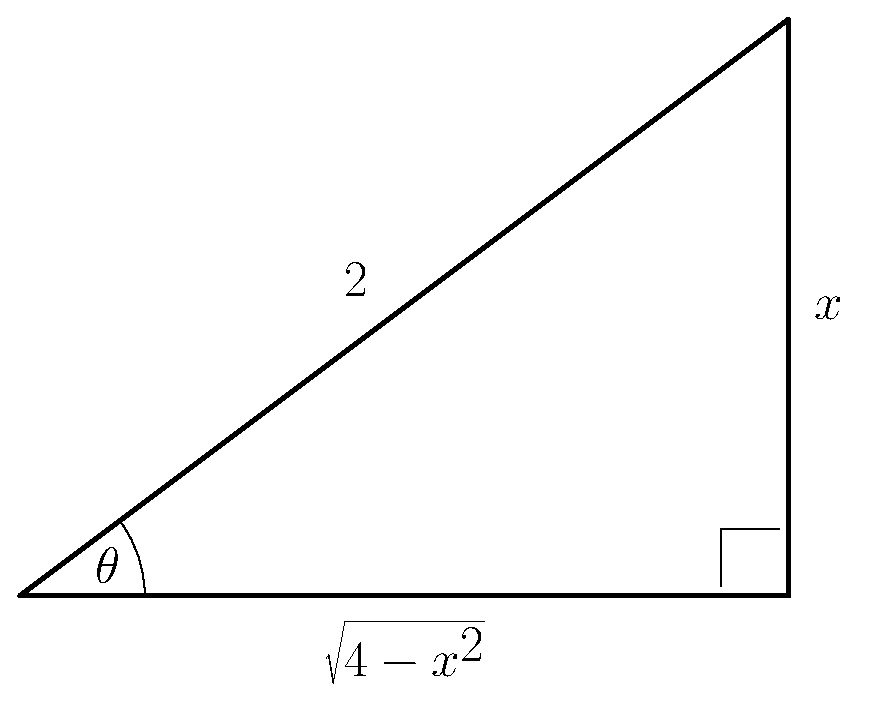
\includegraphics[scale=0.4]{ChapterAntidiff/Figures/sinsubtri}
\end{center}
This makes it easier to know what to substitute for other trig functions of $\theta$.  For example, cosine is the ratio of the adjacent side length to the hypotenuse, so we have:
$$\cos(\theta)=\frac{\sqrt{4-x^2}}{2} $$


\begin{exercise}{
Try One on your own! \Coffeecup \Coffeecup \Coffeecup}
 Evaluate the following antiderivative:

$$\int x^3\left( 16-x^2 \right)^{5/2} \dif x$$  ({\bf Hint:} Recall our methods for integrating powers of sines and cosines!)
\solushun{We have an expression of the form $a^2-x^2$, so we can use a sine substitution and let $x=4\sin(\theta), \dif x=4\cos(\theta)\dif\theta$.
\begin{align*}
\int x^3\left(16-x^2\right)^\frac{5}{2}\dif x&=\int \left(4\sin(\theta)\right)^3\left(16-16\sin^2(\theta)\right)^\frac{5}{2}4\cos(\theta)\dif\theta\\
&=\int 4^3\sin^3(\theta)\left(16\left(1-\sin^2(\theta)\right)\right)^\frac{5}{2}4\cos(\theta)\dif\theta\\
&=\int 4^3\sin^3(\theta)\cdot4^5\left(\cos^2(\theta)\right)^\frac{5}{2}\cdot4\cos(\theta)\dif\theta\\
&=4^9\int \sin^3(\theta)\cdot\cos^5(\theta)\cdot\cos(\theta)\dif\theta\\
&=4^9\int \sin^3(\theta)\cos^6(\theta)\dif\theta\\
\end{align*}
Now we can use our tools for integrating powers of sine and cosine, with $u=\cos(\theta)$ and $\dif u =-\sin(\theta)$.
\begin{align*}
4^9\int \sin^3(\theta)\cos^6(\theta)\dif\theta&=4^9\int \left(\sin^2(\theta)\right)\left(\sin(\theta)\right)\cos^6(\theta)\dif\theta\\
&=4^9\int \left(1-\cos^2(\theta)\right)\left(\sin(\theta)\right)\cos^6(\theta)\dif\theta\\
&=-4^9\int \left(1-u^2\right)u^6\dif u\\
&=-4^9\int u^6-u^8\dif u\\
&=-4^9\left(\frac{1}{7}u^7-\frac{1}{8}u^8\right)+C\\
&=-4^9\left(\frac{1}{7}\cos^7(\theta)-\frac{1}{9}\cos^9(\theta)\right)+C\\
\end{align*}
\begin{wrapfigure}{r}{0.25\textwidth}
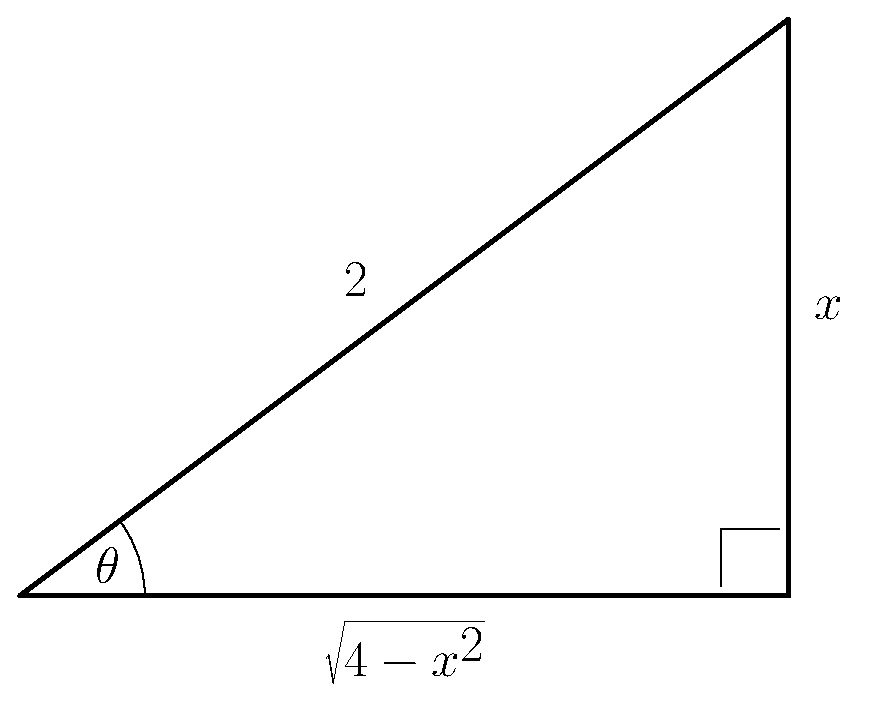
\includegraphics[scale=0.3]{ChapterAntidiff/Figures/sinsubtri}
\end{wrapfigure}
To unwind in terms of $x$, we can use the definition of sine and cosine as side ratios of a triange. If $x=4\sin(\theta)$, we can draw the triangle:\\
From this, you can see that $\cos(\theta)=\frac{\sqrt{4^2-x^2}}{4}$. We can substitute that in for the $\cos(\theta)$'s in the answer:
\begin{align*}
-4^9\left(\frac{1}{7}\cos^7(\theta)-\frac{1}{9}\cos^9(\theta)\right)+C&=-4^9\left(\frac{1}{7}\left(\frac{\sqrt{4^2-x^2}}{4}\right)^7-\frac{1}{9}\left(\frac{\sqrt{4^2-x^2}}{4}\right)^9\right)+C\\
&=-4^9\left(\frac{1}{7}\left(\frac{4\sqrt{1-\frac{x^2}{16}}}{4}\right)^7-\frac{1}{9}\left(\frac{4\sqrt{1-\frac{x^2}{16}}}{4}\right)^9\right)+C\\
&=-4^9\left(\frac{1}{7}\left(\sqrt{1-\frac{x^2}{16}}\right)^7-\frac{1}{9}\left(\sqrt{1-\frac{x^2}{16}}\right)^9\right)+C\\
&=2^{18}\left(\frac{\left(1-\frac{x^2}{16}\right)^{9/2}}{9}-\frac{\left(1-\frac{x^2}{16}\right)^{7/2}}{7}\right)+C\\
\end{align*}
And that's it.
}{3in}
\AnswerKeyEntry{The antiderivative is $2^{18}\left(\frac{\left(1-x^2/16\right)^{9/2}}{9}-\frac{\left(1-x^2/16\right)^{7/2}}{7}\right)+C$}
\end{exercise} 

\subsection{\secant{Secant Substitution}}\label{secantsub} When we see an expression of the form $x^2-a^2$ in the integrand, we think of the identity $\sec^2(\theta)-1=\tan^2(\theta)$, so we use the following substitution:

\FormulaBox{Secant Substitution}{\begin{tabular}{c}
		$x=a\cdot \sec(\theta)$
	\end{tabular}}
    
\begin{example}{A Secant Substitution}\label{secsub}
Suppose we wish to evaluate the following integral: $$\int \frac{1}{x^4-9x^2}\dif x $$  Since $x^4-9x^2=x^2\left(x^2-9\right)$, we use the following substitution: 
\begin{align*}
x&=3\sec\left(\theta\right) \\
\dif x &= 3 \sec\left(\theta\right)\tan\left(\theta\right)\dif \theta 
\end{align*}

We now apply these substitutions to rewrite the integral in terms of $\theta$.

\begin{align*}
\int \frac{1}{x^4-9x^2}\dif x &=\int \frac{1}{x^2\left(x^2-9\right)}\dif x  \\
&=\int \frac{3 \sec\left(\theta\right)\tan\left(\theta\right)}{9\sec^2\left(\theta\right)\left(9\sec^2\left(\theta\right)-9\right)}\dif \theta \\
&=\int \frac{3 \sec\left(\theta\right)\tan\left(\theta\right)}{81\sec^2\left(\theta\right)\tan^2\left(\theta\right)}\dif \theta \\
&=\frac{1}{27}\int \frac{1}{\sec\left(\theta\right)\tan\left(\theta\right)}\dif \theta \\
&=\frac{1}{27}\int\frac{\cos^2\left(\theta\right)}{\sin\left(\theta\right)} \dif \theta \\
&=\frac{1}{27}\int\frac{1-\sin^2\left(\theta\right)}{\sin\left(\theta\right)} \dif \theta \\
&=\frac{1}{27}\int\frac{1}{\sin\left(\theta\right)} \dif \theta-\frac{1}{27}\int \frac{\sin^2\left(\theta\right)}{\sin\left(\theta\right)}\dif \theta \\
&=\frac{1}{27}\int \csc\left(\theta\right) \dif \theta -\frac{1}{27}\int \sin\left(\theta\right) \dif \theta \\
&=-\frac{1}{27}\ln\left|\csc\left(\theta\right)+\cot\left(\theta\right)\right|+\frac{1}{27}\cos\left(\theta\right)+C
\end{align*}
Here we have successfully taken the antiderivative, and now need to just get back to $x$ from $\theta$.  We draw a triangle and label the sides according to our substitution.  In particular, $$\sec\left(\theta\right)=\frac{x}{3}=\frac{\text{hypotenuse}}{\text{adjacent}}$$ so we can let the hypotenuse be $x$ and the adjacent side be 3.
\begin{center}
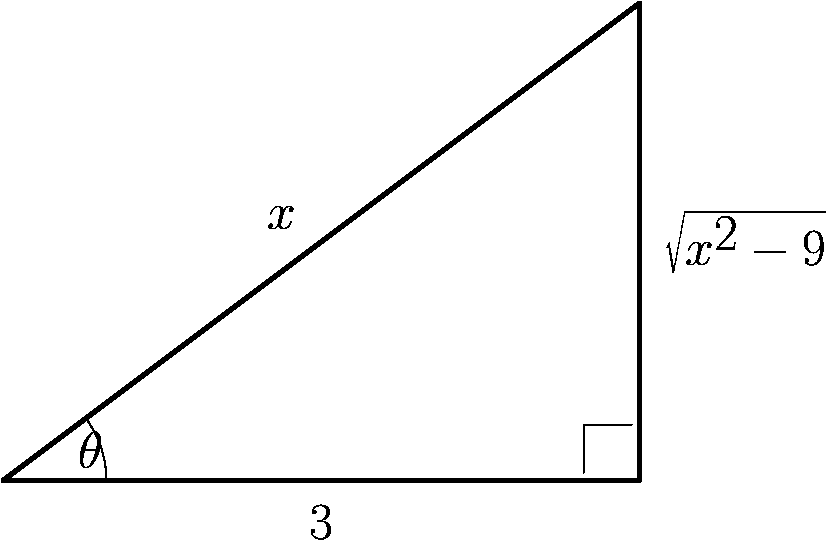
\includegraphics[scale=0.4]{ChapterAntidiff/Figures/sectri_crop}
\end{center}
This enables us to compute the other trig functions using this triangle.  
\end{example}

\begin{exercise}{Getting from $\theta$ back to $x$ \Coffeecup }
Complete the above example by using the triangle to find the values of the other trig functions. \vspace{-.3in}
\begin{center}
\begin{align*}
\cos(\theta)&= \hspace{2in}\\
\cot(\theta)&= \hspace{2in}\\
\csc(\theta)&= \hspace{2in}
\end{align*}
\end{center}

Then plug these expressions back into our antiderivative to get a final answer in terms of $x$ rather than $\theta$.  Make these substitutions and then simplify to verify the final answer shown below.  Show your work below.  \begin{align*}
\int \frac{1}{x^4-9x^2}\dif x &= -\frac{1}{27}\ln\left|\csc\left(\theta\right)+\cot\left(\theta\right)\right|+\frac{1}{27}\cos\left(\theta\right)+C \\
&= \\
&= \\
&= \frac{1}{9x}-\frac{1}{27}\ln\left| \frac{x+3}{\sqrt{x^2-9}}\right|+C
\end{align*}

\end{exercise}

\begin{exercise}{Yes You Can!  Take the Cant Out of Secant! \Coffeecup \Coffeecup \Coffeecup} Evaluate the following antiderivative:
$$\int \sqrt{x^2-4}\dif x.$$
\solushun{We have an expression of the form $x^2-a^2$, so we can use a secant substitution and let $x=2\sec(\theta), \dif x=2\sec(\theta)\tan(\theta)\dif\theta$.
\begin{align*}
\int \sqrt{x^2-4}\dif x&=\int \sqrt{4\sec^2(\theta)-4}\cdot2\sec(\theta)\tan(\theta)\dif \theta\\
&=\int \sqrt{4\sec^2(\theta)-4}\cdot2\sec(\theta)\tan(\theta)\dif \theta\\
&=\int 2\sqrt{\sec^2(\theta)-1}\cdot2\sec(\theta)\tan(\theta)\dif \theta\\
&=4\int \sqrt{\tan^2(\theta)}\cdot\sec(\theta)\tan(\theta)\dif \theta\\
&=4\int \sec(\theta)\tan^2(\theta)\dif \theta\\
\end{align*}
Using the Pythagorean Identity, we can split the integral:
\begin{align*}
4\int \sec(\theta)\tan^2(\theta)\dif \theta&=4\int \sec(\theta)\left(\sec^2(\theta)-1\right)\dif \theta\\
&=4\int \sec^3(\theta)-\sec(\theta)\dif \theta\\
&=4\left[\int \sec^3(\theta)\dif \theta-\int \sec(\theta)\dif \theta\right]
\end{align*}
From previous exercises, we can evaluate these as:
$$
4\left[\int \sec^3(\theta)\dif \theta-\int \sec(\theta)\dif \theta\right]=4\left[\frac{\sec(\theta)\tan(\theta)+\ln\left|\sec(\theta)+\tan(\theta)\right|}{2}-\ln\left|\sec(\theta)+\tan(\theta)\right|\right]
$$
To unwind, note that $x=2\sec(\theta)$ so that $\sec(\theta)=\frac{x}{2}$, which gives us enough information to draw a right triangle (try it) and find the side ratios, giving us $\tan(\theta)=\frac{\sqrt{x^2-4}}{2}$.
\begin{align*}
4\left[\frac{\sec(\theta)\tan(\theta)+\ln\left|\sec(\theta)+\tan(\theta)\right|}{2}-\ln\left|\sec(\theta)+\tan(\theta)\right|\right]+C\\
=4\left[\frac{\frac{x}{2}\cdot\frac{\sqrt{x^2-4}}{2}+\ln\left|\frac{x}{2}+\frac{\sqrt{x^2-4}}{2}\right|}{2}-\ln\left|\frac{x}{2}+\frac{\sqrt{x^2-4}}{2}\right|\right]+C\\
=4\left[\frac{\frac{x\sqrt{x^2-4}}{4}+\ln\left|\frac{x+\sqrt{x^2-4}}{2}\right|}{2}-\ln\left|\frac{x+\sqrt{x^2-4}}{2}\right|\right]+C\\
=\frac{x\sqrt{x^2-4}}{2}+2\ln\left|\frac{x+\sqrt{x^2-4}}{2}\right|-4\ln\left|\frac{x+\sqrt{x^2-4}}{2}\right|+C\\
=\frac{x\sqrt{x^2-4}}{2}-2\ln\left|\frac{x+\sqrt{x^2-4}}{2}\right|+C
\end{align*}
We can clean this up a bit by absorbing part of the logarithm into the constant:
\begin{align*}
\frac{x\sqrt{x^2-4}}{2}-2\ln\left|\frac{x+\sqrt{x^2-4}}{2}\right|+C&=\frac{x\sqrt{x^2-4}}{2}-\left(2\ln\left|x+\sqrt{x^2-4}\right|-2\ln|2|\right)+C\\
&=\frac{x\sqrt{x^2-4}}{2}-2\ln\left|x+\sqrt{x^2-4}\right|+C
\end{align*}}{4in}
\AnswerKeyEntry{Exercise \ref{reappear}.\ref{seccubed} will be helpful!  The antiderivative is $\frac{x\sqrt{x^2-4}}{2}-2\ln|x+\sqrt{x^2-4}|+C$.}
\end{exercise}

\subsection{\tangent{Tangent Substitution}} When we see an expression of the form $a^2+x^2$ or $x^2+a^2$ (which are the same) in the integrand, we think of the identity $\tan^2(\theta)+1=\sec^2(\theta)$, so we use the following substitution:

\FormulaBox{Tangent Substitution}{\begin{tabular}{c}
		$x=a\cdot \tan(\theta)$
	\end{tabular}
}

\begin{exercise}{Revisiting an Old Friend \Coffeecup \Coffeecup}
\begin{itemize}
\item Recall the derivative of arctangent:
$$\frac{\dif}{\dif x}\left(\arctan(x)\right)=\hspace{3in} $$
\solushun{$$\frac{1}{1+x^2}$$}{0in}

\item We should be able to reverse the above by taking the antiderivative of the right-hand side.  Perform this antiderivative using the substitution $x=\tan(\theta)$:

$$\int \frac{1}{1+x^2}\dif x = \hspace{3.2in} $$
\solushun{Let $x=\tan(\theta), \dif x=\sec^2(\theta)$.
\begin{align*}
\int \frac{1}{1+x^2}\dif x&=\int \frac{1}{1+tan^2(\theta)}\sec^2(\theta)\dif\theta\\
&=\int \frac{\sec^2(\theta)}{\sec^2(\theta)}\dif\theta\\
&=\int 1\dif\theta\\
&=\theta+C\\
&=\arctan(x)+C
\end{align*}}{2in}

\end{itemize}
\end{exercise}

\subsection{Preprocessing with Algebra or $u$-sub}  Often we need to do a little algebra and/or $u$-sub to get the integrand into a form where we can then perform trig sub.


\begin{exercise}{A Bit of Algebra to Help Us \Coffeecup \Coffeecup \Coffeecup }

\begin{itemize}
\item Explain why the two following expressions are equal: $$(4x^2+1)^2=16\left(x^2+\left(\frac{1}{2}\right)^2\right)^2$$
\solushun{\begin{align*}
(4x^2+1)^2&=\left(4\left(x^2+\frac{1}{4}\right)\right)^2\\
&=\left(4\right)^2\left(x^2+\left(\frac{1}{2}\right)^2\right)^2\\
&=16\left(x^2+\left(\frac{1}{2}\right)^2\right)^2
\end{align*}}{1in}

\item Use the equality above along with a tangent substitution to evaluate the following antiderivative:

$$\int \frac{1}{(4x^2+1)^2} \dif x$$
\solushun{\begin{align*}
\int \frac{1}{(4x^2+1)^2} \dif x&=\int \frac{1}{16\left(x^2+\left(\frac{1}{2}\right)^2\right)^2} \dif x\\
&\text{Let $x=\frac{1}{2}\tan(\theta), \dif x=\frac{1}{2}\sec^2(\theta)$}.\\
&=\int \frac{1}{16\left(\frac{1}{4}\tan^2(\theta)+\left(\frac{1}{2}\right)^2\right)^2}\cdot\frac{1}{2}\sec^2(\theta)\dif\theta\\
&=\frac{1}{32}\int \frac{\sec^2(\theta)}{\left(\frac{1}{4}\tan^2(\theta)+\left(\frac{1}{2}\right)^2\right)^2}\dif\theta\\
&=\frac{1}{32}\int \frac{\sec^2(\theta)}{\left(\frac{1}{4}\sec^2(\theta)\right)^2}\dif\theta\\
&=\frac{1}{32}\int \frac{\sec^2(\theta)}{\frac{1}{16}\sec^4(\theta)}\dif\theta\\
&=\frac{1}{2}\int \frac{1}{\sec^2(\theta)}\dif\theta\\
&=\frac{1}{2}\int \cos^2(\theta)\dif\theta\\
&=\frac{1}{2}\int \frac{1+\cos(2\theta)}{2}\dif\theta\\
&=\frac{1}{2}\int \frac{1}{2}+\frac{1}{2}\cos(2\theta)\dif\theta\\
&=\frac{1}{2}\left( \frac{1}{2}\theta+\frac{1}{4}\sin(2\theta)+C\right)\\
&= \frac{1}{4}\theta+\frac{1}{8}\sin(2\theta)+C\\
&= \frac{1}{4}\theta+\frac{1}{4}\sin(\theta)\cos(\theta)+C\\
&\text{Since, $\tan(\theta)=2x$, we construct a triangle to obtain $\cos(\theta)$ and $\sin(\theta)$.}\\
&\sin(\theta))=\frac{2x}{\sqrt{4x^2-1}}, \cos(\theta))=\frac{1}{\sqrt{4x^2-1}}\\
&=\frac{1}{4}\arctan(2x)+\frac{1}{4}\frac{2x}{\sqrt{4x^2-1}}\cdot\frac{1}{\sqrt{4x^2-1}}+C\\
&=\frac{1}{4}\arctan(2x)+\frac{x}{8x^2-2}+C\\
\end{align*}}{4in}
\end{itemize}
\end{exercise}

A trick from algebra that is often used \cts{with trigonometric substitution} is completing the square.  You might need to complete the square to get it into a form where a trig sub will work.  

\begin{example}{Completing the Square}
Suppose we wish to find an antiderivative for the function $\left(x^2+x-1\right)^{-2}$.  We begin by completing the square on the quadratic polynomial:

\begin{align*}
x^2+x-1&=x^2+x+\frac{1}{4}-\frac{1}{4}-1 \\
       &=\left(x+\frac{1}{2}\right)^2-\frac{5}{4} \\ 
\end{align*}

We now use the substitution that this quadratic motivates.  Namely, we pick $a=\frac{\sqrt{5}}{2}$ since we want its square to be five-fourths.  Where $x$ used to go in the problems above, we now have an $x+\frac{1}{2}$.  Thus our substitution is $ x+\frac{1}{2}=\frac{\sqrt{5}}{2}\sec(\theta)$, or more explicitly:

$$  x=\frac{\sqrt{5}}{2}\sec(\theta)-\frac{1}{2} $$

Taking the derivative of both sides with respect to $\theta$ shows that 

$$  \mathtt{d}x=\frac{\sqrt{5}}{2}\sec(\theta)\tan(\theta) \mathtt{d}\theta $$

\end{example}

\begin{exercise}{Completing the Example \Coffeecup \Coffeecup \Coffeecup}

Use the substitutions suggested in the example above to find the antiderivative.

$$\int \frac{1}{(x^2+x-1)^2} \mathtt{d}x = \hspace{4in} $$

\AnswerKeyEntry{The antiderivative is $-\frac{1}{5}\frac{2x+1}{x^2+x-1}+\frac{4\sqrt{5}}{25}\ln\left(\frac{2x+1+\sqrt{5}}{2\sqrt{x^2+x-1}}\right)+C$.  Note that one can expand using properties of logarithms and then rename $C$ as $C-\frac{4\sqrt{5}}{25}\ln(2)$ since it is anyhow just an arbitrary constant.  Thus, we can slightly clean up the answer to become $-\frac{1}{5}\frac{2x+1}{x^2+x-1}+\frac{4\sqrt{5}}{25}\ln\left(2x+1+\sqrt{5}\right)-\frac{2\sqrt{5}}{25}\ln\left(x^2+x-1\right)+C.$}

\solushun{With $x+\frac{1}{2}=\frac{\sqrt{5}}{2}\sec(\theta)$, and $\dif x=\frac{\sqrt{5}}{2}\sec(\theta)\tan(\theta) \dif\theta$, we have:
\begin{align*}
\int \frac{1}{(x^2+x-1)^2} \dif x &= \int \frac{1}{(x+\frac{1}{2})^2-\frac{5}{4}} \dif x = \int \frac{\frac{\sqrt{5}}{2}\sec(\theta)\tan(\theta)}{\left(\frac{\sqrt{5}}{2}\sec(\theta)\right)^2-\frac{5}{4}} \dif\theta \\
&=\frac{\sqrt{5}}{2}\int \frac{\sec(\theta)\tan(\theta)}{\frac{5}{4}\sec^2(\theta)-\frac{5}{4}} \dif\theta\\
&=\frac{2\sqrt{5}}{5}\int \frac{\sec(\theta)\tan(\theta)}{\tan^2(\theta)} \dif\theta\\
&=\frac{2\sqrt{5}}{5}\int \frac{\sec(\theta)}{\tan(\theta)} \dif\theta\\
&=\frac{2\sqrt{5}}{5}\int\csc(\theta)\dif\theta\\
&=-\frac{2}{\sqrt{5}}\ln|\csc(\theta)+\cot(\theta)|+C\\
\end{align*}
Using the initial substitution $\sec(\theta)=\frac{2}{\sqrt{5}}\left(x+\frac{1}{2}\right)$, we can draw a triangle and derive the other sides to get $\csc\theta=\frac{2x+1}{2\sqrt{x^2+x-1}}$ and $\cot\theta=\frac{\sqrt{5}}{2\sqrt{x^2+x-1}}$
\begin{align*}
-\frac{2}{\sqrt{5}}\ln\left|\csc(\theta)+\cot(\theta)\right|+C&=-\frac{2}{\sqrt{5}}\ln\left|\frac{2x+1}{2\sqrt{x^2+x-1}}+\frac{\sqrt{5}}{2\sqrt{x^2+x-1}}\right|+C\\
&=\frac{-2\ln\left|\frac{2x+1+\sqrt{5}}{2\sqrt{x^2+x-1}}\right|}{\sqrt{5}}+C\\
&=\frac{-2\ln\left|2x+1+\sqrt{5}\right|+2\ln\left|2\sqrt{x^2+x-1}\right|}{\sqrt{5}}+C\\
&=\frac{-2\ln\left|2x+1+\sqrt{5}\right|+\ln\left(\left|2\sqrt{x^2+x-1}\right|\right)^2}{\sqrt{5}}+C\\
&=\frac{-2\ln\left|2x+1+\sqrt{5}\right|+\ln\left|4x^2+4x-4\right|}{\sqrt{5}}+C\\
&=\frac{-2\ln\left|2x+1+\sqrt{5}\right|+\ln\left|4(x+\frac{1+\sqrt{5}}{2})(x+\frac{1-\sqrt{5}}{2})\right|}{\sqrt{5}}+C\\
&=\frac{-2\ln\left|2x+1+\sqrt{5}\right|+\ln\left|4\cdot\frac{1}{2}(2x+1+\sqrt{5})\cdot\frac{1}{2}(2x+1-\sqrt{5})\right|}{\sqrt{5}}+C\\
&=\frac{-2\ln\left|2x+1+\sqrt{5}\right|+\ln\left|(2x+1+\sqrt{5})(2x+1-\sqrt{5})\right|}{\sqrt{5}}+C\\
&=\frac{-2\ln\left|2x+1+\sqrt{5}\right|+\ln\left|(2x+1+\sqrt{5})\right|+\ln\left|(2x+1-\sqrt{5})\right|}{\sqrt{5}}+C\\
&=\frac{\ln\left|(2x+1-\sqrt{5})\right|-\ln\left|2x+1+\sqrt{5}\right|}{\sqrt{5}}+C\\
\end{align*}}{4in}\end{exercise}

\begin{exercise}{Try One On Your Own \Coffeecup \Coffeecup \Coffeecup} Evaluate the following antiderivative: $$\int \frac{x}{\sqrt{2x^2-4x-7}}\dif x$$
\solushun{Completing the square first, we get:
$$\int \frac{x}{\sqrt{2x^2-4x-7}}\dif x= \int \frac{x}{\sqrt{2\left(x^2-2x+1\right)-2-7}}\dif x= \int \frac{x}{\sqrt{2\left(x-1\right)^2-9}}\dif x$$
We want an expression of the form $a^2\sec^2\theta-a^2$, so if we let $(x-1)=\frac{3}{\sqrt{2}}\sec\theta$, we get the desired result.
\begin{align*}
\int \frac{x}{\sqrt{2\left(x-1\right)^2-9}}\dif x&=\int \frac{\frac{3}{\sqrt{2}}\sec(\theta)+1}{\sqrt{2\left(\frac{3}{\sqrt{2}}\sec\theta\right)^2-9}}\cdot\frac{3}{\sqrt{2}}\sec(\theta)\tan(\theta) \dif x\\
&=\int \frac{\frac{9}{2}\sec(\theta)+\frac{3}{\sqrt{2}}}{\sqrt{2\left(\frac{9}{2}\sec^2(\theta)\right)-9}}\cdot\sec(\theta)\tan(\theta) \dif x\\
&=\int \frac{\frac{9}{2}\sec(\theta)+\frac{3}{\sqrt{2}}}{\sqrt{9\sec^2(\theta)-9}}\cdot\sec(\theta)\tan(\theta) \dif x\\
&=\int \frac{\frac{9}{2}\sec(\theta)+\frac{3}{\sqrt{2}}}{\sqrt{9\tan^2(\theta)}}\cdot\sec(\theta)\tan(\theta) \dif x\\
&=\int \frac{\frac{9}{2}\sec(\theta)+\frac{3}{\sqrt{2}}}{3\tan^(\theta)}\cdot\sec(\theta)\tan(\theta) \dif x\\
&=\int\frac{3}{2}\sec^2(\theta)+\frac{1}{\sqrt{2}}\sec(\theta) \dif x\\
&=\frac{3}{2}\tan(\theta)+\frac{1}{\sqrt{2}}\ln\left|\sec(\theta)+\tan(\theta)\right|+C\\
\end{align*}
Using our initial substitution, we have $\sec(\theta)=\frac{\sqrt{2}}{3}(x-1)$. Drawing a triangle with hypotenuse $\sqrt{2}(x-1)$ and bottom leg $3$, we can determine $\tan(\theta)=\frac{\sqrt{2x^2-4x-7}}{3}$. Plugging these in for the trig functions gives us:
\begin{align*}
\frac{3}{2}\tan(\theta)+\frac{1}{\sqrt{2}}\ln\left|\sec(\theta)+\tan(\theta)\right|+C&=\frac{3}{2}\frac{\sqrt{2x^2-4x-7}}{3}+\frac{1}{\sqrt{2}}\ln\left|\frac{\sqrt{2}}{3}(x-1)+\frac{\sqrt{2x^2-4x-7}}{3}\right|+C\\
&=\frac{\sqrt{2x^2-4x-7}}{2}+\frac{1}{\sqrt{2}}\ln\left|\frac{\sqrt{2}x-\sqrt{2}+\sqrt{2x^2-4x-7}}{3}\right|+C\\
\end{align*}
We can clean this result up a bit by noticing that we can split the logarithm on the right hand side and that $\ln3$ is a constant that we can roll into $C$.
\begin{align*}
&=\frac{\sqrt{2x^2-4x-7}}{2}+\frac{1}{\sqrt{2}}\ln\left|\frac{\sqrt{2}x-\sqrt{2}+\sqrt{2x^2-4x-7}}{3}\right|+C\\
&=\frac{\sqrt{2x^2-4x-7}}{2}+\frac{1}{\sqrt{2}}\left(\ln\left|\sqrt{2}x-\sqrt{2}+\sqrt{2x^2-4x-7}\right|-\ln|3|\right)+C\\
&=\frac{\sqrt{2x^2-4x-7}}{2}+\frac{1}{\sqrt{2}}\ln\left|\sqrt{2}x-\sqrt{2}+\sqrt{2x^2-4x-7}\right|+C
\end{align*}
Furthermore, we can multiply and divide everything in the logarithm by $\sqrt{2}$ as well, and pull out $\ln\sqrt{2}$ as another constant.
\begin{align*}
&=\frac{\sqrt{2x^2-4x-7}}{2}+\frac{1}{\sqrt{2}}\ln\left|\sqrt{2}x-\sqrt{2}+\sqrt{2x^2-4x-7}\right|+C\\
&=\frac{\sqrt{2x^2-4x-7}}{2}+\frac{1}{\sqrt{2}}\ln\left|\frac{\sqrt{2}\left(\sqrt{2}x-\sqrt{2}+\sqrt{2x^2-4x-7}\right)}{\sqrt{2}}\right|+C\\
&=\frac{\sqrt{2x^2-4x-7}}{2}+\frac{1}{\sqrt{2}}\left(\ln\left|2x-2+\sqrt{4x^2-8x-14}\right|-\ln|\sqrt{2}|\right)+C\\
&=\frac{\sqrt{2x^2-4x-7}}{2}+\frac{1}{\sqrt{2}}\ln\left|2x-2+\sqrt{4x^2-8x-14}\right|+C
\end{align*}
Lastly, we can rationalize the denominator and factor out $\frac{1}{2}$.
\begin{align*}
&=\frac{\sqrt{2x^2-4x-7}}{2}+\frac{1}{\sqrt{2}}\ln\left|2x-2+\sqrt{4x^2-8x-14}\right|+C\\
&=\frac{\sqrt{2x^2-4x-7}}{2}+\frac{\sqrt{2}}{2}\ln\left|2x-2+\sqrt{4x^2-8x-14}\right|+C\\
&=\frac{1}{2}\left(\sqrt{2x^2-4x-7}+\sqrt{2}\ln\left|2x-2+\sqrt{4x^2-8x-14}\right|\right)+C
\end{align*}.
Thus, our final expression:
$$\int \frac{x}{\sqrt{2x^2-4x-7}}\dif x=\frac{1}{2}\left(\sqrt{2x^2-4x-7}+\sqrt{2}\ln\left|2x-2+\sqrt{4x^2-8x-14}\right|\right)+C$$}{6.5in}
\end{exercise}

\section{Partial Fraction Decomposition}

In this section, we will combine the techniques of all previous sections and learn how to antidifferentiate \antider{rational functions}!

\begin{exercise}{What is a Rational Function Again? \Coffeecup}
What is the definition of a \emph{rational function}?
\solushun{A rational function is a function that is expressed as a ratio, with some power of $x$ in the denominator. Think a polynomial divided by a polynomial.\\}{.5in}
\end{exercise}

A \antider{partial fraction decomposition} (PFD) is a way to decompose a \partialfractions{rational function} (a polynomial divided by a polynomial) as a sum of simpler \integ{rational functions}.  This is purely an algebraic trick that fundamentally does not involve calculus.  It is useful in many contexts!  Here we apply it to (of course) finding antiderivatives. Typically, a given rational function is too challenging to antidifferentiate as is. Once we break it up into smaller pieces via PFD, it becomes manageable.

The fundamental idea is simple. If we have a fraction that has more than one factor in the denominator, we can rewrite it as a sum of fractions whose denominators have the original denominator as their least common multiple. 
\begin{exercise}{Trying This with Integers Before We Go to Polynomials \Coffeecup}
 Consider the fraction $\frac{1}{6}$.  We notice that the denominator, six, is equal to two times three.  Thus, we attempt to write one-sixth as a sum of fractions whose denominators are two and three.
 
Find integers $A$ and $B$ such that:
$$\frac{1}{6}=\frac{A}{2}+\frac{B}{3} $$
Check your answer by adding the fractions on the right hand side back together to verify you get one-sixth. 
\solushun{
$$3A+2B=1$$
$$A=\frac{1-2B}{3}$$
Let $B=2$. Then $A=\frac{1-4}{3}=-1$.
$$-\frac{1}{2}+\frac{2}{3}=\frac{-3+4}{3\cdot 2}=\frac{1}{6}$$
}{.5in}
\end{exercise}

\subsection{Warming Up with a Small Example}\label{PotatoFryDip}

Partial fraction decomposition is the same idea, except we are working with polynomials rather than just integers.

\begin{example}{Our First Decomposition!}\label{OurFirstPotatoFryDip}
 To decompose the fraction $\frac{1}{x^2-1}$, we first factor the denominator into $x^2-1=(x-1)(x+1)$.  Thus, we look for an expression of the form  $$ \frac{1}{x^2-1}=\frac{A}{x-1}+\frac{B}{x+1}$$
for some numbers $A$ and $B$.  To find such $A$ and $B$, we multiply both sides by $x^2-1$ to produce the polynomial equation  $$1=A(x+1)+B(x-1) $$

Since we want the expressions to be equal for all values of $x$, we pick convenient values of $x$ to plug in to solve for $A$ and $B$.  
\begin{itemize}
\item Set $x=1$: $$1=A\cdot (2) + B \cdot (0) \implies A=\frac{1}{2}$$
\item Set $x=-1$: $$1=A\cdot (0) + B \cdot (-2) \implies B=-\frac{1}{2}$$
\end{itemize}
At last, we have obtained the partial fraction decomposition! $$\frac{1}{x^2-1}=\frac{\frac{1}{2}}{x-1}-\frac{\frac{1}{2}}{x+1}$$
\end{example}

\begin{exercise}{Checking Our Work \Coffeecup} Take the right-hand side of the above equation and add the two fractions together by finding a common denominator. Verify that their sum is the original rational function $\frac{1}{x^2-1}$.
\solushun{\begin{align*}
\frac{\frac{1}{2}}{x-1}-\frac{\frac{1}{2}}{x+1}&=\frac{\frac{1}{2}(x+1)-\frac{1}{2}(x-1)}{(x-1)(x+1)}\\
&=\frac{\frac{x}{2}+\frac{1}{2}-\left(\frac{x}{2}-\frac{1}{2}\right)}{x^2-1}\\
&=\frac{\frac{x}{2}+\frac{1}{2}-\frac{x}{2}+\frac{1}{2}}{x^2-1}\\
&=\frac{1}{x^2-1}
\end{align*}}{1in}
\end{exercise}
\begin{example}{Finding the Same PFD by Expanding and Equating Coefficients}\label{57Varieties}
We repeat the above example but demonstrate an alternate way to find our coefficients.  Recall the equation $$1=A(x+1)+B(x-1) $$  In the previous example, we proceeded by plugging in numerical values for $x$.  Instead, we could fully multiply out the polynomials and combine like terms.  This produces $$1=(A+B)x+(A-B) $$  We can pad the left-hand side with a degree one term with coefficient zero to put both sides in the form ``number times $x$ plus number''.  $$0x+1=(A+B)x+(A-B) $$  Now we can construct a system of two equations in two unknowns by equating one coefficient at a time.  Specifically, we build it as:
\begin{center}
\begin{tabular}{|r l|c|l r|} \hline & & & & \\ 
Degree zero coefficient of LHS = &\hspace{-.18in} Degree zero coefficient of RHS & $\implies $ & $1 =$ & \hspace{-.18in} $A-B$ \\ & & & &  \\ \hline & & & &  \\ 
Degree one coefficient of LHS = & \hspace{-.18in} Degree one coefficient of RHS & $\implies $ & $0 =$ & \hspace{-.18in} $A+B$ \\ & & & &  \\ \hline 
\end{tabular}
\end{center}
The resulting linear system in two equations and two unknowns can then be solved via any applicable method (substitution, elimination, matrices, etc). 
\end{example}
\begin{exercise}{Solve the System \Coffeecup}
Solve the linear system of two equations and two unknowns in the example above.  Verify you obtain the same values for $A$ and $B$ that we found in Example \ref{PotatoFryDip}.\ref{OurFirstPotatoFryDip}.
\vspace*{1in}
\end{exercise}
\begin{exercise}{Using a PFD to Find an Antiderivative \Coffeecup \Coffeecup } \begin{itemize}
\item  Find an antiderivative of $\frac{1}{x^2-1}$ by antidifferentiating $$\frac{\frac{1}{2}}{x-1}-\frac{\frac{1}{2}}{x+1}$$
\solushun{
\begin{align*}
\int\frac{\frac{1}{2}}{x-1}-\frac{\frac{1}{2}}{x+1}\dif x&=\int\frac{\frac{1}{2}}{x-1}\dif x-\int\frac{\frac{1}{2}}{x+1}\dif x\\
&=\frac{1}{2}\int\frac{1}{x-1}\dif x-\frac{1}{2}\int\frac{1}{x+1}\dif x\\
&=\frac{1}{2}\ln|x-1|-\frac{1}{2}\ln|x+1|+C\\
&=\frac{1}{2}\left(\ln|x-1|-\ln|x+1|\right)+C\\
&=\frac{1}{2}\ln\left|\frac{x-1}{x+1}\right|+C\\
&=\ln\left| \sqrt{\frac{x-1}{x+1}}\right|+C
\end{align*}
}{3in}
\item Verify the answer is the same as what you would get if you had taken the antiderivative of  $\frac{1}{x^2-1}$ using the trigonometric substitution $x=\sec(\theta)$.
\solushun{With $x=\sec(\theta)$ and $\dif x = \sec(\theta)\tan(\theta)\dif\theta$ we have:
\begin{align*}
\int\frac{1}{x^2-1}\dif x&=\int\frac{1}{\sec^2(\theta)-1}\sec(\theta)\tan(\theta)\dif\theta\\
&=\int\frac{1}{\tan^2(\theta)}\sec(\theta)\tan(\theta)\dif\theta\\
&=\int\frac{\sec(\theta)}{\tan(\theta)}\dif\theta\\
&=\int\frac{1}{\cos(\theta)}\cdot\frac{\cos(\theta)}{\sin(\theta)}\dif\theta\\
&=\int\frac{1}{\sin(\theta)}\dif\theta\\
&=\int\csc(\theta)\dif\theta\\
&=-\ln|\csc(\theta)+\cot(\theta)|+C\\
\end{align*}
Constructing a triangle with $x=\sec(\theta)$, we can determine $\csc(\theta)=\frac{x}{\sqrt{x^2-1}}$ and $\cot(\theta)=\frac{1}{\sqrt{x^2-1}}$. So we have:
\begin{align*}
-\ln|\csc(\theta)+\cot(\theta)|+C&=-\ln\left|\frac{x}{\sqrt{x^2-1}}+\frac{1}{\sqrt{x^2-1}}\right|+C\\
&=-\ln\left|\frac{x+1}{(\sqrt{x-1})(\sqrt{x+1})}
\right|+C\\
&=-\ln\left|\frac{\sqrt{x+1}}{\sqrt{x-1}}\right|+C\\
&=\ln\left|\left(\sqrt{\frac{x+1}{x-1}}\right)^{-1}\right|+C\\
&=\ln\left|\sqrt{\frac{x-1}{x+1}}\right|+C\\
\end{align*}
And we have the same result.\\
}{3in}
\AnswerKeyEntry{Using properties of logarithms, both answers should be able to be put in the form $\ln\left| \sqrt{\frac{x-1}{x+1}}\right|+C$}
\end{itemize}
\end{exercise}
It turns out there are three strange things that can happen when finding a PFD, namely: 
\begin{enumerate}
\item The degree of the numerator is greater than or equal to the degree of the denominator. 
\item The denominator has one or more irreducible quadratic factors (where irreducible quadratic means a degree two polynomial that has no real roots).
\item The denominator has one or more repeated factors.
\end{enumerate}

Each has a particular workaround.  Below, we describe these methods and show a corresponding hideous example that demonstrates all of these steps.  

\begin{exercise}{Reminding Ourselves of Some Language \Coffeecup}
\begin{itemize}
\item What exactly does \emph{irreducible quadratic} mean?
\solushun{A quadratic that can't be factored into real roots.\\}{.5in}
\item Give an example of a quadratic polynomial that is irreducible.
\solushun{$x^2+x+1$\\}{.5in}
\item Give an example of a quadratic polynomial that is not irreducible.
\solushun{$x^2+2x+1$\\}{.5in}
\item Is the polynomial $x^2$ an irreducible quadratic?  Explain why or why not.
\solushun{No. It has real roots $x=0$.\\}{.5in}
\vspace*{.5in}
\end{itemize}
\end{exercise}


\subsection{The General Method of PFD}
The process for performing a partial fraction decomposition of $\frac{p(x)}{q(x)}$ is as follows:

\begin{enumerate}
\item {\bf Polynomial Long Division:} If the degree of $p(x)$ is not strictly smaller than the degree of $q(x)$, start by performing polynomial \partialfractions{long division} to split the fraction into a quotient and remainder.  In the remainder term, the numerator will now have degree less than the denominator. 

\item {\bf Factor Denominator:} Factor the denominator into a product of powers of linear and irreducible quadratic polynomials.

\item {\bf Set Up Terms in the Summation:}
\begin{enumerate}
\item {\bf Linear Factors:}  If the denominator is divisible by $(x-r)^n$ for some real number $r$ and positive natural number $n$, we build terms that look like

$$\frac{A_1}{x-r}+\frac{A_2}{(x-r)^2}+\frac{A_3}{(x-r)^3}+\cdots+\frac{A_n}{(x-r)^n} $$

where the $A_i$ represent unknown real constants.  That is, you use all consecutive powers of a linear factor as denominators and have arbitrary constants as numerators.
\item {\bf Irreducible Quadratic Factors:}  Let $b$ and $c$ be real numbers and suppose $x^2+bx+c$ is an irreducible quadratic.  If the denominator is divisible by $(x^2+bx+c)^n$ for some positive natural number $n$, we build terms that look like

$$\frac{A_1x+B_1}{x^2+bx+c}+\frac{A_2x+B_2}{(x^2+bx+c)^2}+\frac{A_3x+B_3}{(x^2+bx+c)^3}+\cdots+\frac{A_nx+B_n}{(x^2+bx+c)^n} $$

where the $A_i$ and $B_i$ represent unknown real constants.  That is, you use all consecutive powers of a linear factor as denominators and have arbitrary constants as numerators.

\end{enumerate}


\item {\bf Clear Denominators:} Multiply each side of your equation by the denominator $q(x)$ to clear all fractions.

\item {\bf Solve for Unknowns:} Solve for the unknown constants by plugging in convenient values of $x$ (since we want the expression to be true for all values of $x$).  The roots of $q(x)$ are always good choices for $x$ values, but other friendly numbers like zero or one are also often helpful.


\item {\bf Plug Values Back into the Previously Unknown Numerators:} Plug your constants back in to conclude the equality of your original rational expression with its PFD.

\end{enumerate}


\begin{example}{An Epic PFD}

We now find the partial fraction decomposition of the rational function $$ r(x)=\frac{x^7+8 x^6+25 x^5+52 x^4+79 x^3+13 x^2-61 x+81}{x^6+9 x^5+28 x^4+36 x^3+27 x^2+27 x}$$

This rational function has quotient $x-1$ and remainder $6 x^5+44 x^4+88 x^3+13 x^2-34 x+81$ upon \remainder{long division}.  So, for our first step in the decomposition we have 

$$r(x)=x-1+\frac{6 x^5+44 x^4+88 x^3+13 x^2-34 x+81}{x^6+9 x^5+28 x^4+36 x^3+27 x^2+27 x}$$

We now ignore the quotient and work on breaking up the fractional piece.  The denominator is divisible by $x$, so we factor that out.  Next, we use the Rational Root Theorem to form a list of possible roots and divide off the corresponding factors as we find them.  Working out all the algebra, we conclude the denominator factors as $$x^6+9 x^5+28 x^4+36 x^3+27 x^2+27 x=x (x+3)^3 (x^2+1)$$

In this particular setting, $x$, $x+3$, $(x+3)^2$, and $(x+3)^3$ are the relevant powers of linear factors. The factor $x^2+1$ is the only irreducible quadratic.  ({\bf Note:} $(x+3)^2$ is not an irreducible quadratic term; it is a common mistake to consider it so.  It is a power of a linear term and should be treated as such.)  We now set up our sum.

$$ \frac{6 x^5+44 x^4+88 x^3+13 x^2-34 x+81}{x (x+3)^3 (x^2+1)} = \frac{A}{x}+\frac{B}{x+3} +\frac{C}{(x+3)^2} + \frac{D}{(x+3)^3} + \frac{Ex+F}{x^2+1} $$
Since fractions are a pain, we get rid of them!  Multiplying both sides by $x (x+3)^3 (x^2+1)$, our equation becomes
$$ 6 x^5+44 x^4+88 x^3+13 x^2-34 x+81$$ 
$$ = A (x+3)^3 (x^2+1)+Bx (x+3)^2 (x^2+1) +Cx (x+3) (x^2+1) + Dx (x^2+1) + (Ex+F)x (x+3)^3 $$

We now solve for our unknown coefficients.  It is highly convenient to set $x=0$. This produces the equation $ 81= A (3)^3 $ which implies $A=3$.  Similarly, we set $x=-3$. This produces the equation $$6 (-3)^5+44 (-3)^4+88 (-3)^3+13 (-3)^2-34 (-3)+81=D(-3) ((-3)^2+1)$$ which simplifies to $ 30=D(-30) $ which implies $D=-1$.  We have now run out of the most convenient values to choose for $x$, namely the roots of the denominator.  At this point, we unfortunately need to do something messy!  We can either plug in less than optimal values of $x$, for example $x=1$, then $x=-1$, then $x=2$, etc, and solve the resulting simultaneous system of equations that results.  Or, we can multiply out the polynomials and equate coefficients one degree at a time (the method of Example \ref{PotatoFryDip}.\ref{57Varieties}).  Carrying out either of these methods will produce

$$ B=2, C=1, E=1, F=-5 $$

At last, we plug the values for the constants $A,B,C,D,E,$ and $F$ back into the original decomposition (with quotient).  Our final PFD is 

$$ \frac{x^7+8 x^6+25 x^5+52 x^4+79 x^3+13 x^2-61 x+81}{x^6+9 x^5+28 x^4+36 x^3+27 x^2+27 x} = x-1 + \frac{3}{x} + \frac{2}{x + 3} + \frac{1}{(x + 3)^2} - \frac{1}{(x + 3)^3} + \frac{x - 5}{x^2 + 1} $$ 

\end{example}

\begin{exercise}{ Identifying the Steps of PFD \Coffeecup}
In the ridiculous example above, label each of the six steps of partial fraction decomposition.  Where exactly does each step occur?
\end{exercise}

\begin{exercise}{ Which Type of Numerator Goes Where? \Coffeecup}
In the above example, notice that the factor $(x+3)^2$ corresponded to a term of the form $$\frac{C}{(x+3)^2}$$ and not a term of the form $$\frac{Cx+D}{(x+3)^2}.$$

Why was this the case?

\vspace*{1in}

\end{exercise}

Well, that's the process of partial fraction decomposition!  Why are we doing it in a calculus course?  Because a generic rational function is really hard to integrate, but the partial fraction decomposition is made up of simpler terms that are much easier to integrate.  Let's find the antiderivative of that beast above!  

\begin{example}{Return of the Son of \emph{Using a PFD to Find an Antiderivative}}

We apply our PFD to compute the following antiderivative:
\begin{align*}
 \int  &\left(\frac{x^7+8 x^6+25 x^5+52 x^4+79 x^3+13 x^2-61 x+81}{x^6+9 x^5+28 x^4+36 x^3+27 x^2+27 x}\right) \dif x \\
&=\int \left(x-1 + \frac{3}{x} + \frac{2}{x + 3} + \frac{1}{(x + 3)^2} - \frac{1}{(x + 3)^3} + \frac{x - 5}{x^2 + 1}\right) \dif x\\
&=\frac{x^2}{2}-x+3\ln(x)  +2\ln(x+3) + -\frac{1}{x+3}   + \frac{1}{2(x + 3)^2} +\int \frac{x}{x^2 + 1} \dif x+ \int \frac{-5}{x^2 + 1} \dif x\\
&=\frac{x^2}{2}-x+3\ln(x)  +2\ln(x+3) + -\frac{1}{x+3}   + \frac{1}{2(x + 3)^2}  + \frac{1}{2}\ln(x^2+1) -5 \arctan(x)
\end{align*}

Oh, and um, plus $C$.
\end{example}

\subsection{Sweet PFD \partialfractions{Flow Chart}}

 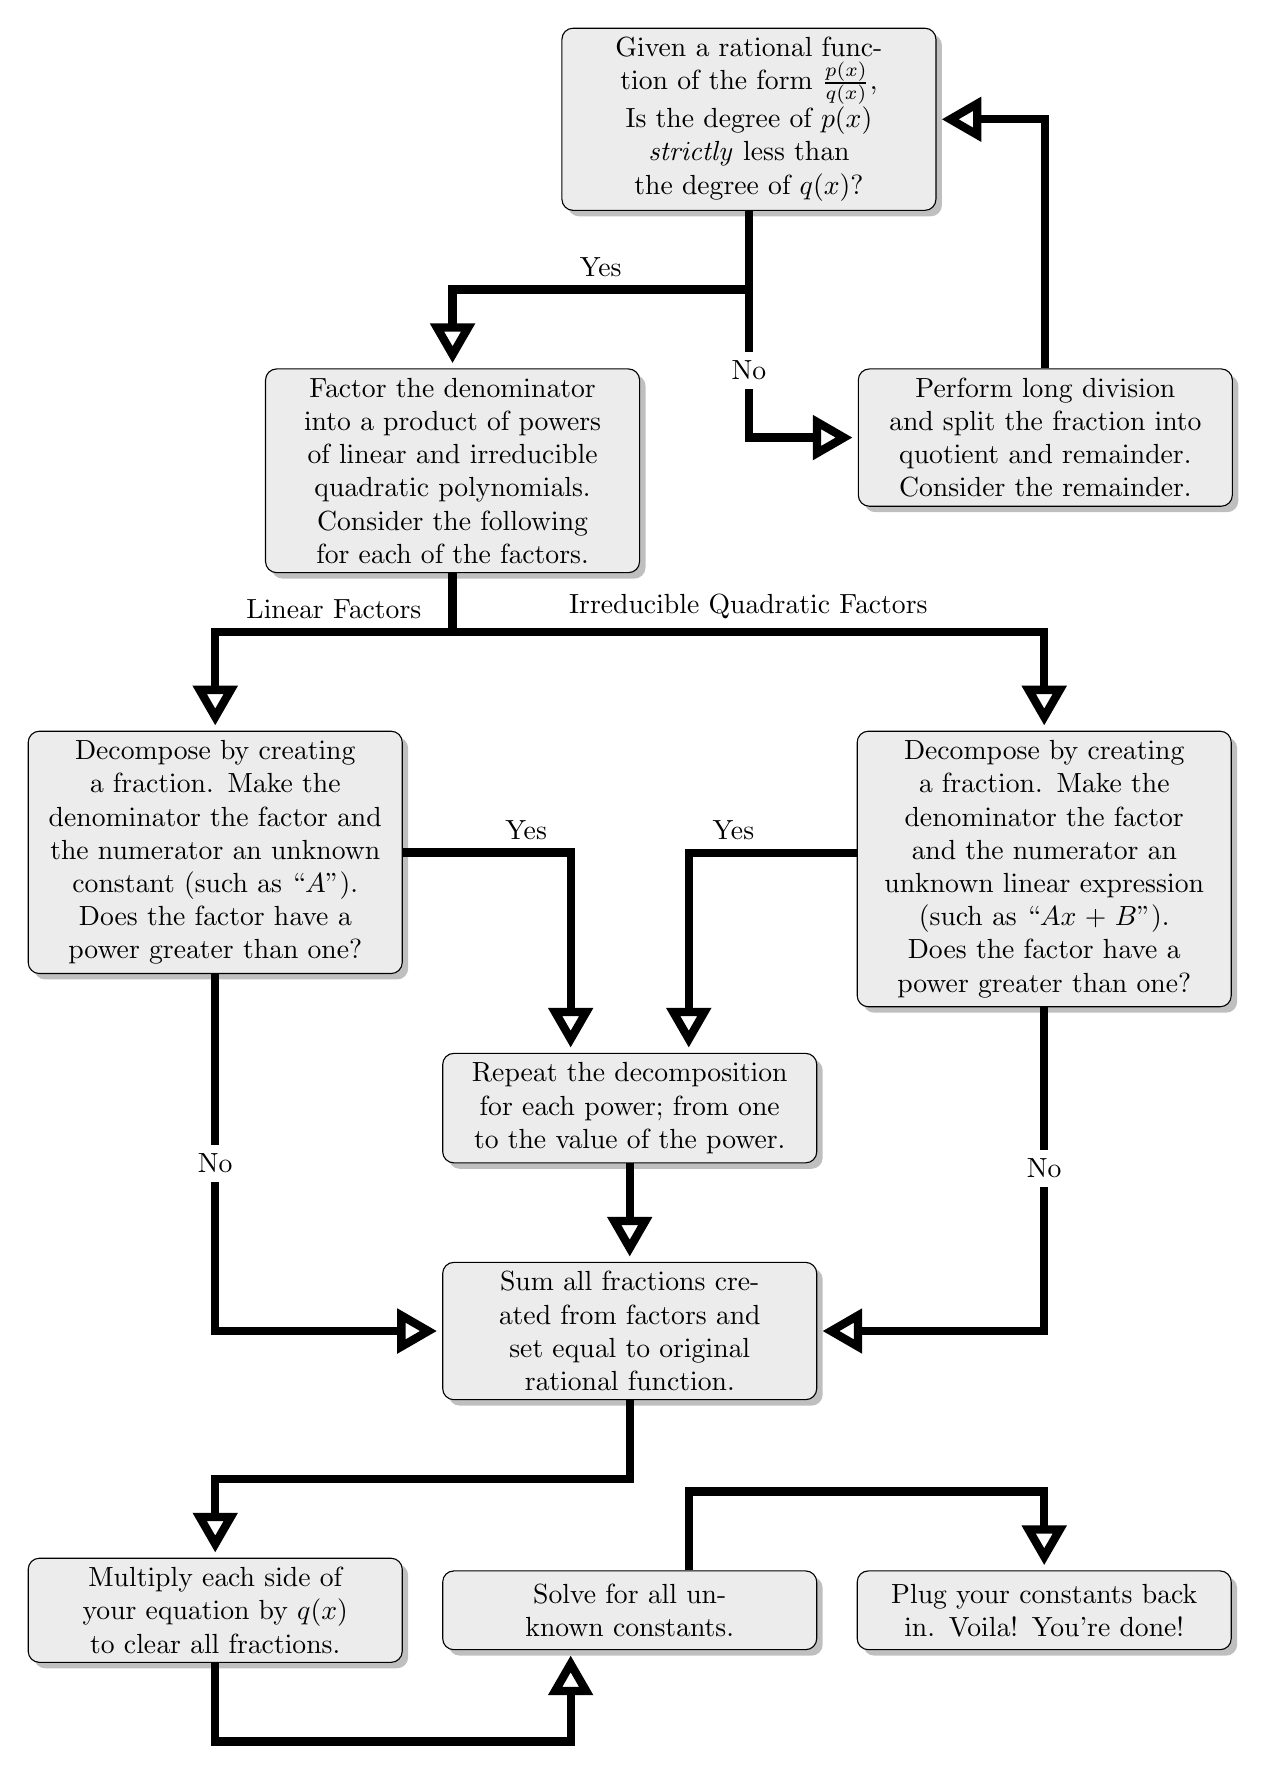
\begin{tikzpicture}[
      >=latex',
      auto
    ]
    
    \tikzstyle{box} = [rectangle, rounded corners, minimum width=4.75cm, minimum height=1cm, text centered, text width=4.25cm, draw=black, fill=gray!15, drop shadow]
    
    \tikzstyle{arrow} = [thick,>=stealth,arrowhead=5mm,->]
    
    \node [box] (given) {
    	Given a rational function of the form $\frac{p(x)}{q(x)}$, \\
        Is the degree of $p(x)$ \textit{strictly} less than the degree of $q(x)$?
        };
        
	\node [box]  (factor) [node distance=2cm and -1cm,below left=of given] {Factor the denominator into a product of powers of linear and irreducible quadratic polynomials. \\
    Consider the following for each of the factors.};
    \node [box] (P1Big) [node distance=2cm and -1cm,below right=of given] {Perform long division and split the fraction into quotient and remainder. Consider the remainder.};    
    
    \node [box]  (linear) [node distance=2cm and -1.75cm,below left=of factor] {Decompose by creating a fraction. Make the denominator the factor and the numerator an unknown constant (such as ``$A$''). \\
    Does the factor have a power greater than one?};
    \node [box]  (irreducible) [node distance=2cm and 2.75cm, below right= of factor] {Decompose by creating a fraction. Make the denominator the factor and the numerator an unknown linear expression (such as ``$Ax+B$'').\\
    Does the factor have a power greater than one?};
    
    \node [box] (multPower) [node distance =1cm and .5cm, below right= of linear] {Repeat the decomposition for each power; from one to the value of the power.};
    
    \node [box] (sum) [node distance=1.25cm, below =of multPower] {Sum all fractions created from factors and set equal to original rational function.};
    
    \node [box] (mult) [node distance=2cm and .5cm, below left =of sum] {Multiply each side of your equation by $q(x)$ to clear all fractions.};
    \node [box] (solve) [node distance=.5cm, right =of mult] {Solve for all unknown constants.};
    \node [box] (finish) [node distance=.5cm, right =of solve] {Plug your constants back in. Voila! You're done!};

       
    
    \draw [->, >=open triangle 60, ultra thick,line width= 3pt, shorten >=2pt] (given) -- ($(given.south)+(0,-1)$) -| (factor) node[above,pos=0.25] {Yes} ;
    \draw [->, >=open triangle 60, ultra thick,line width= 3pt, shorten >=2pt] (given) -- ($(given.south)+(0,-1)$) |- (P1Big) node[above,fill=white,pos=0.35] {No} ;
    
    \draw [->, >=open triangle 60, ultra thick,line width= 3pt, shorten >=2pt] (P1Big) -- ($(P1Big.north)+(0,2.75)$) |- (given.east);
    
    \draw [->, >=open triangle 60, ultra thick,line width= 3pt, shorten >=2pt] (factor) -- ($(factor.south)+(0,-.75)$) -| (linear) node[above,pos=0.25] {Linear Factors} ;
    \draw [->, >=open triangle 60, ultra thick,line width= 3pt, shorten >=2pt] (factor) -- ($(factor.south)+(0,-.75)$) -| (irreducible) node[above,pos=0.25] {Irreducible Quadratic Factors} ;
    
    \draw [->, >=open triangle 60, ultra thick, line width=3pt, shorten >=2pt] (linear.east) -- ($(linear.east)+(1,0)$) -| ($(multPower.north)+(-.75,0)$) node[above,pos=0.25] {Yes};
    \draw [->, >=open triangle 60, ultra thick, line width=3pt, shorten >=2pt] ($(irreducible.west)+(0,.2)$) -- ($(irreducible.west)+(-1,.2)$) -| ($(multPower.north)+(.75,0)$) node[above,pos=0.25] {Yes};
     \draw [->, >=open triangle 60, ultra thick, line width=3pt, shorten >=2pt] ($(multPower.south)$) -- ($(sum.north)$);
    
    \draw [->, >=open triangle 60, ultra thick, line width=3pt, shorten >=2pt] (linear.south) -- ($(linear.south)+(0,-3)$) |- (sum.west) node[above,fill=white,pos=-.1] {No};
    \draw [->, >=open triangle 60, ultra thick, line width=3pt, shorten >=2pt] (irreducible.south) -- ($(irreducible.south)+(0,-3)$) |- (sum.east) node[above,fill=white,pos=-.3] {No};
    
    \draw [->, >=open triangle 60, ultra thick, line width=3pt, shorten >=2pt] (sum.south) -- ($(sum.south)+(0,-1)$) -| (mult.north);
    
    \draw [->, >=open triangle 60, ultra thick, line width=3pt, shorten >=2pt] (mult.south) -- ($(mult.south)+(0,-1)$) -| ($(solve.south)+(-.75,0)$);
    \draw [->, >=open triangle 60, ultra thick, line width=3pt, shorten >=2pt] ($(solve.north)+(0.75,0)$) -- ($(solve.north)+(0.75,1)$) -| (finish.north);


\end{tikzpicture}

\begin{exercise}{Now you cry! I mean, try!  \Coffeecup \Coffeecup \Coffeecup }
Find the following antiderivatives.  Keep in mind that not every step of PFD will necessarily occur in every problem!

\begin{itemize}

\item $ \displaystyle
\int\frac{1}{x^2-9x+20}\dif x $
\solushun{
Let's start by breaking up the fraction. We can factor $x^2-9x+20$ into $(x-5)(x-4)$.
$$\frac{1}{x^2-9x+20}=\frac{A}{x-5}+\frac{B}{x-4}$$
Multiplying by the common denominator gives
$$1=A(x-4)+B(x-5)$$
First let $x=5$:
$$1=A(5-4)+B(5-5)=A$$
Then let $x=4$:
$$1=A(4-4)+B(4-5)=-B$$
$$A=1, B=-1$$
Now we can proceed with our integral:
\begin{align*}
\int\frac{1}{x-5}-\frac{1}{x-4}\dif x&=\ln|x-5|-\ln|x-4|+C\\
&=\ln\left|\frac{x-5}{x-4}\right|+C
\end{align*}
}{3in}

\item $\displaystyle \int  \frac{1}{x^4-9} \dif x $
\solushun{$x^4-9$ factors to $(x^2+3)(x^2-3)$. $(x^2-3)$ further factors to $(x-\sqrt{3})(x+\sqrt{3})$. So our partial fraction decomposition is:
$$\frac{1}{x^4-9}=\frac{Ax+B}{x^2+3}+\frac{C}{x-\sqrt{3}}+\frac{D}{x+\sqrt{3}}$$
Multiplying both sides by the common denominator gives:
$$1=(Ax+B)(x^2-3)+C(x^2+3)(x+\sqrt{3})+D(x^2+3)(x-\sqrt{3})$$
We can let $x=\sqrt{3}$:
$$1=(Ax+B)(3-3)+C(3+3)(\sqrt{3}+\sqrt{3})+D(3+3)(\sqrt{3}-\sqrt{3})$$
$$1=C(6)(2\sqrt{3})=12\sqrt{3}C$$
So $C=\frac{1}{12\sqrt{3}}$.
Let $x=-\sqrt{3}$:
$$1=(Ax+B)(3-3)+C(3+3)(-\sqrt{3}+\sqrt{3})+D(3+3)(-\sqrt{3}-\sqrt{3})$$
$$1=D(6)(-2\sqrt{3})=-12\sqrt{3}D$$
So $D=-\frac{1}{12\sqrt{3}}$.
To get $A$ and $B$, substitute everything we have and multiply out the polynomial:
$$1=(Ax+B)(x^2-3)+\frac{1}{12\sqrt{3}}(x^2+3)(x+\sqrt{3})+\frac{-1}{12\sqrt{3}}(x^2+3)(x-\sqrt{3})$$
$$1=Ax^3-3Ax+Bx^2-3B+\frac{1}{12\sqrt{3}}(x^3+x^2\sqrt{3}+3x+3\sqrt{3})-\frac{1}{12\sqrt{3}}(x^3-x^2\sqrt{3}+3x-3\sqrt{3})$$
$$1=Ax^3-3Ax+Bx^2-3B+\frac{1}{12\sqrt{3}}(x^3+x^2\sqrt{3}+3x+3\sqrt{3})-\frac{1}{12\sqrt{3}}(x^3-x^2\sqrt{3}+3x-3\sqrt{3})$$
$$1=Ax^3-3Ax+Bx^2-3B+\frac{x^2}{12}+\frac{1}{4}+\frac{x^2}{12}+\frac{1}{4}$$
$$1=Ax^3-3Ax+Bx^2-3B+\frac{x^2}{6}+\frac{1}{2}$$
Before proceeding, note that $A$ is the only coefficient with an $x^3$ term on either side. Since there is no $x^3$ on the LHS, and none on the RHS to cancel out $Ax^3$, we know $A=0$. We can substitute that in to simplify further:
$$1=Bx^2-3B+\frac{x^2}{6}+\frac{1}{2}$$
Now, note that the $x^2$ term on the LHS is $0$, so $Bx^2+\frac{1}{6}x^2=0$, which tells us $B=-\frac{1}{6}$. We can check that by looking at the constant term, which is $1$. $-3B+\frac{1}{2}=1$. Using $B=-\frac{1}{6}:-3\frac{-1}{6}+\frac{1}{2}=\frac{1}{2}+\frac{1}{2}=1$.
Plug all the terms back into the original PFD:
\begin{align*}
\int \frac{-\frac{1}{6}}{x^2+3}+\frac{\frac{1}{12\sqrt{3}}}{x-\sqrt{3}}+\frac{-\frac{1}{12\sqrt{3}}}{x+\sqrt{3}} \dif x&=-\frac{1}{6}\int\frac{1}{x^2+3}\dif x+\frac{1}{12\sqrt{3}}\int\frac{1}{x-\sqrt{3}}\dif x-\frac{1}{12\sqrt{3}}\int\frac{1}{x+\sqrt{3}} \dif x\\
&=-\frac{1}{12}\ln|x^2+3|+\frac{1}{12\sqrt{3}}\ln|x-\sqrt{3}|-\frac{1}{12\sqrt{3}}\ln|x+\sqrt{3}|+C\\
&=-\frac{1}{12}\ln|x^2+3|+\frac{1}{12\sqrt{3}}\ln\left|\frac{x-\sqrt{3}}{x+\sqrt{3}}\right|+C\\
\end{align*}
}{3in}

\item $\displaystyle \int  \frac{x^4}{x^2+1} \dif x $
\solushun{ We use polynomial long division, so that 
$$\frac{x^4}{x^2+1}=x^2-1+\frac{1}{x^2+1}$$
Then, the antiderivative is fairly straightfowarad:
\begin{align*}
    \int\frac{x^4}{x^2+1}\dif x&=\int x^2-1+\frac{1}{x^2+1}\dif x\\
    &=\frac{1}{3}x^3-x+\frac{1}{2}\ln|x^2+1|+C
\end{align*}}{3in}

\item $\displaystyle \int  \frac{2}{x^5+2x^3+x} \dif x $
\solushun{We start by factoring the fraction:
$$\frac{2}{x^5+2x^3+x}=\frac{1}{(x)(x^4+2x^2+1)}=\frac{1}{(x)(x^2+1)^2}$$
Our PFD breaks apart into:
$$2\left(\frac{1}{x^5+2x^3+x}\right)=2\left(\frac{A}{x}+\frac{Bx+c}{x^2+1}+\frac{Dx+E}{(x^2+2)^2}\right)$$
From here, the simplest approach is to multiply both sides by the least common denominator and compare terms of like power, and then solve the resulting system of equations.
$$1=A(x^2+1)^2+(Bx+C)(x)(x^2+1)+(Dx+E)(x)$$
We have an easy win by first setting $x=0:1=A$.
$$1=x^4+2x^2+1+Bx^4+Bx^2+Cx^3+Cx+Dx^2+Ex$$
Collecting like terms and comparing to the LHS, we have:
\begin{align*}
(B+1)x^4&=0x^4\\
(C)x^3&=0x^3\\
(2+B+D)x^2&=0x^2\\
(E)x&=0x
\end{align*}
Solving these systems of equations, we get $A=1, B=-1, C=0, D=-1, E=0$, and our PFD becomes:
$$2\left(\frac{1}{x^5+2x^3+x}\right)=2\left(\frac{1}{x}+\frac{-1x}{x^2+1}+\frac{-1x}{(x^2+2)^2}\right)$$
Solving our antiderivative now is much easier:
\begin{align*}
\int2\left(\frac{1}{x}+\frac{-x}{x^2+1}+\frac{-x}{(x^2+1)^2}\right)\dif x&=2\int\frac{1}{x}-\frac{x}{x^2+1}-\frac{x}{(x^2+1)^2}\dif x\\
&=2\left(\ln|x|-\frac{1}{2}\ln|x^2+1|+\frac{1}{2}\frac{1}{x^2+1}+C\right)\\
&=2\ln|x|-\ln|x^2+1|+\frac{1}{x^2+1}+C
\end{align*}}{3in}

\item $\displaystyle \int  \frac{x-2}{x^3+x^2+3 x-5} \dif x $
\solushun{Our PFD is:
$$\frac{x-2}{x^3+x^2+3x-5}=\frac{x-2}{(x-1)(x^2+2x+5)}=\frac{A}{x-1}+\frac{Bx+C}{x^2+2x+5}$$
Then we can solve for $A, B$ and $C$:
\begin{align*}
    x-1&=A(x^2+2x+5)+(Bx+C)(x-1)\\
    &=Ax^2+2Ax+5A+Bx^2-Bx+Cx-C\\
\end{align*}
Grouping by like power terms:
\begin{align*}
    (A+B)x^2&=0x^2\\
    (2A-B+C)x&=x\\
    (5A-C)&=-1
\end{align*}
}{4in}

\end{itemize}
\AnswerKeyEntry{\textbullet The function $\frac{1}{x^2-9x+20}$ has $\ln\left|\frac{x-5}{x-4}\right|+C$ as its antiderivative.  
\textbullet The factorization $x^4-9=\left(x^2+3\right)\left(x-\sqrt{3}\right)\left(x+\sqrt{3}\right)$ will produce the following setup: $$\frac{1}{x^4-9}=\frac{Ax+B}{x^2+3}+\frac{C}{x-\sqrt{3}}+\frac{D}{x+\sqrt{3}} $$ in which you can then solve for the coefficients and antidifferentiate. 
\textbullet The function $\frac{x^4}{x^2+1}$ has an irreducible quadratic for a denominator. However, the degree of the numerator is not smaller than the degree of the denominator.  Thus, polynomial long division is the only step of PFD that is required in this case. 
\textbullet The antiderivative of $\frac{2}{x^5+2x3+x}$ is $$2\ln|x|-\ln\left| x^2+1\right|+\frac{1}{x^2+1}$$
\textbullet The PFD will produce $$ \frac{x-2}{x^3+x^2+3x-5}=\frac{-\frac{1}{8}}{x-1}+\frac{\frac{1}{8}x+\frac{11}{8}}{x^2+2x+5}$$ While the first term is easy to integrate, the second is quite tricky!  To hack through it, split it as follows: $$\frac{\frac{1}{8}x+\frac{11}{8}}{x^2+2x+5}=\frac{\frac{1}{8}x+\frac{1}{8}}{x^2+2x+5}+\frac{\frac{10}{8}}{x^2+2x+5} $$  The first fraction can then be integrated via $u$-sub, while the second can be done via trig sub after completing the square on the denominator.}
\end{exercise}

\begin{exercise}{Revisiting an Old Friend \Coffeecup \Coffeecup \Coffeecup}
Recall Example \ref{secantsub}.\ref{secsub}, where we found the antiderivative of $$\frac{1}{x^4-9x^2}$$ via trig sub.  Find this antiderivative again but via PFD!  Verify your answer is compatible with what trig sub produced.  
\solushun{The fraction breaks up into $\frac{1}{x^2(x-3)(x+3)}$, so we construct the partial fractions: $$\frac{A}{x}+\frac{B}{x^2}+\frac{C}{x-3}+\frac{D}{x+3}$$. Clearing the denominator produces:
$$A(x)(x-3)(x+3)+B(x-3)(x+3)+C(x^2)(x+3)+D(x^2)(x-3)=1$$. We can clear out the fractions by settings $x$ equal to the roots of the denominator:
\begin{align*}
    x=0 &: -9B = 1 \implies B=-\frac{1}{9}\\
    x=3 &: C(9)(6) = 1 \implies C=\frac{1}{54}\\
    x=-3 &: D(9)(-6) = 1 \implies D=-\frac{1}{54}\\
\end{align*}
Since $A$ has an $x^3$ power and nothing else does, we know $A=0$.
So our integral is $$\int\frac{1}{9x^2}+\frac{1}{54(x-3)}-\frac{1}{54(x+3)}\dif x$$
Solving this produces
\begin{align*}
    \frac{1}{9x}+\frac{1}{54}\ln|x-3|-\frac{1}{54}\ln|x+3|&=\frac{1}{9x}+\frac{1}{54}\left(\ln|x-3|-\ln|x+3|\right)\\
    &=\frac{1}{9x}+\frac{1}{54}\ln\left|\frac{x-3}{x+3}\right|
\end{align*}
}{4in}
\AnswerKeyEntry{For $\frac{1}{x^4-9x^2}$, keep in mind that $x^2$ is not an irreducible quadratic factor but rather a repeated linear factor.  The PFD and integration will produce $$\frac{1}{9x}+\frac{1}{54}\ln\left|\frac{x-3}{x+3}\right|+C $$ }
\end{exercise}

\section{Chapter Summary}

In this chapter, we tackled a very difficult question, namely \begin{center}
\emph{Given a function $f(x)$, how does one find an antiderivative?}
\end{center}  Though there are many functions out there that do not have a closed form antiderivative, we explored {\bf five} techniques that can get you there in a great many cases!  Here are brief descriptions of the five:

\begin{enumerate}
\item {\bf U-substitution:} Try to clean up an integral by making a substitution of the form $u=g(x)$.  Often $g(x)$ is chosen to be the inner function in some function composition appearing in the integrand.  

\item {\bf Integration by Parts:} This is the product rule for antiderivatives.  We identify two factors in the integrand and call one $u$ while the other is called $\dif v$.  We then apply the IBP formula: $$\int u\dif v=uv-\int v\dif u.$$  In general, one tries to pick $u$ to be something that is cleaner when differentiated and $\dif v$ to be something we can antidifferentiate.
\item {\bf Products of sines and cosines:} Any expression of the form $$\int \sin^n(x)\cos^m(x) \dif x$$
for $n,m\in \mathbb{N}$ can be integrated by using the appropriate trig identities based on the parity of $n$ and $m$.
\item {\bf Trigonometric Substitution:} If you see quadratic polynomials in your integrand, you can likely clean things up with a trigonometric substitution.  In particular, 
\begin{center}
\begin{tabular}{|c|c|c|} \hline 
 If you see... &   ...make the substitution... & ...because...  \\ \hline 
 $a^2-x^2$ &  $  x=a \sin\left(\theta\right) $ & $a^2-a^2\sin^2\left(\theta\right)=a^2\cos^2\left(\theta\right) $ \\
 $a^2+x^2$ &  $  x=a \tan\left(\theta\right) $ & $a^2+a^2\tan^2\left(\theta\right)=a^2\sec^2\left(\theta\right) $ \\
$x^2-a^2$ &  $  x=a \sec\left(\theta\right) $ & $a^2\sec^2\left(\theta\right)-a^2=a^2\tan^2\left(\theta\right) $ \\ \hline
\end{tabular}
\end{center}

\item {\bf Partial Fraction Decomposition:}  This is the general method by which we can integrate any expression of the form $$\int \frac{p(x)}{q(x)}\dif x $$ where $p(x)$ and $q(x)$ are polynomials.
\end{enumerate}

Don't forget that you can check your work on any antiderivative by differentiating your answer.  The result should be the original integrand!


\section{Mixed Practice}

\subsection{Warm Ups}
These are good problems for reinforcing the vocabulary and foundational concepts of this chapter.
\begin{exercise}{\Coffeecup }
Find the antiderivative of $\frac{1}{1+x}$ using the substitution $u=1+x$.
\AnswerKeyEntry{$\ln\left(1+x\right)+C$}
\solushun{ $\int{\frac{1}{1+x} \dif x} \newline$
Let $u=1+x$ then $\dif u=\dif x \newline$
so $\int{\frac{1}{1+x} \dif x} =\int{\frac{1}{u} \dif u}= \ln\left(u\right)+C=\ln\left(1+x\right)+C$ \\ }{0in}
\end{exercise}

\begin{exercise}{\Coffeecup \Coffeecup }
Find the antiderivative 

$$\int \frac{\sqrt{x}}{\sqrt{x}+1}\dif x $$ using the substitution $u=\sqrt{x}+1$.
\AnswerKeyEntry{$x+ -2\sqrt{x}+2\ln{|\sqrt{x}+1|}+C$}
\solushun{ $\int \frac{\sqrt{x}}{\sqrt{x}+1}dx \newline$
Let $u=\sqrt{x}+1$ then $du = 1/2 x^{-1/2} dx$ so $2 x^{1/2} du=dx \newline$
so $\int \frac{\sqrt{x}}{\sqrt{x}+1}dx = \int \frac{\sqrt{x}}{u}(2 x^{1/2} du)=
2 \int {\frac{x}{u} du}$ but since $u=\sqrt{x}+1 \Rightarrow x=(u-1)^2$ we have
$2 \int {\frac{x}{u} du}=2 \int {\frac{(u-1)^2}{u} du}=2 \int {\frac{u^2-2u+1}{u} du}=2 \int {(u-2+\frac{1}{u}) du}= 2(u^2/2-2u +\ln{|u|})+C \newline$
$ = (\sqrt{x}+1)^2 -4(\sqrt{x}+1) + 2\ln{|\sqrt{x}+1|}+C = x -2\sqrt{x}+2\ln{|\sqrt{x}+1|}+C$\\ }{0in}
\end{exercise}

\begin{exercise}{\Coffeecup \Coffeecup }
Compute the exact value of the following definite integral:
$$ \int_{x=1}^{x=\sqrt{3}} \frac{1}{\sqrt{x^2+1}} \dif x. $$
\AnswerKeyEntry{$\ln \left| \frac{ 2+\sqrt{3}}{\sqrt{2} +1} \right|$}
\solushun{ Use $x=\tan{\theta}$ then $\dif x=\sec^2{\theta} \dif \theta$. Also, $x^2 = \tan^2{\theta} $ and $\tan^2{\theta} +1 = \sec^2{\theta}$. So
$$\int_{1}^{\sqrt{3}}{\frac{1}{\sqrt{x^2+1}} \dif x} = \int_{\theta=\frac{\pi}{4}}^{\theta=\frac{\pi}{3}}{\frac{1}{\sqrt{\tan^2{\theta}}+1} \cdot \sec^2{\theta} \dif \theta}= \int_{\theta=\frac{\pi}{4}}^{\theta=\frac{\pi}{3}}{\frac{1}{\sec{\theta}} \cdot \sec^2{\theta} \dif \theta}
=\int_{\theta=\frac{\pi}{4}}^{\theta=\frac{\pi}{3}}{\sec{\theta} \dif \theta}
$$
$$=\ln|\sec{\theta}+\tan{\theta}| \Biggr|_{\theta=\frac{\pi}{4}}^{\theta=\frac{\pi}{3}}= \ln|\sec( \pi/3)+\tan(\pi/3)| - \ln|\sec(\pi/4)+\tan(\pi/4)| 
=\ln \left| \frac{ 2+\sqrt{3}}{\sqrt{2} +1} \right|
$$\\ }{0in}
\end{exercise}

\begin{exercise}{\Coffeecup \Coffeecup}
Calculate the antiderivative: $$ \int {\frac{1}{x^4-x^2}\dif x}$$ via partial fraction decomposition.
\AnswerKeyEntry{$\frac{1}{2}\ln{|x-1|}-\frac{1}{2}\ln{|x+1|} +\frac{1}{x} +C$}
\solushun{First let $\frac{1}{x^4-x^2} = \frac{1}{x^2(x-1)(x+1)}= \frac{A}{x-1}+\frac{B}{x+1}+\frac{C}{x}+\frac{D}{x^2}$  then we have $1= Ax^2(x+1)+Bx^2(x-1)+Cx(x+1)(x-1)+D(x+1)(x-1)$ \\
Let $x=0$ then $1=D(1)(-1) = -D$ so $D=-1$ \\
Let $x=1$ then $1=A(2)$ so $A=\frac{1}{2}$ \\
Let $x=-1$ then $1 = B(-2)$ so $B=-\frac{1}{2}$ \\
We can find C using the degree 3 coefficients of the equation \\$1= Ax^2(x+1)+Bx^2(x-1)+Cx(x+1)(x-1)+D(x+1)(x-1)$ \\so we have $0 = A+B+C \Rightarrow -A-B = C \Rightarrow -\frac{1}{2} +\frac{1}{2} =C \Rightarrow C=0$ \\
So we have $$\int{\frac{1}{x^4-x^2}dx} = \int{\frac{\frac{1}{2}}{x-1}+\frac{-\frac{1}{2}}{x+1}+\frac{0}{x}+\frac{-1}{x^2}dx}=\frac{1}{2}\ln{|x-1|}-\frac{1}{2}\ln{|x+1|} +\frac{1}{x} +C$$
\\ }{0in}
\end{exercise}


\subsection{Sample Test Problems}

\begin{exercise}{\Coffeecup \Coffeecup }
 Consider $\int {\cos^{13}{x}\sin^{5}{x} \dif x}$.
\begin{itemize}
\item  Can you compute this integral using $u=\cos{x}$?  Explain.
\solushun{ Yes, use one factor of $\sin{x} $ for the $\dif u$. Specifically, $u=\cos{x}$ implies $ \dif u=-\sin{x} \dif x$ and use  $\sin^2{x}=1-\cos^2{x}$.
\\ }{0in}

\item  Can you compute this integral using $u=\sin(x)$?  Explain.
    \solushun{ Yes, using $\cos(x)$ for the $\dif u$. Specifically, $u=\sin(x)$ implies $\dif u = \cos(x)\dif x$. Then $\int {\cos^{13}{x}\sin^{5}{x} \dif x}=\int \cos^{12}(x)\sin^5(x)\cos(x)\dif x = \int (1-u^2)^6 u^5\dif u$. \\ }{0in}

\item Which of the two above substitutions will be easier to use?  Carry out the integration, using the easier of the two.
\solushun{ 
        The first substitution is easier. Proceeding with $u=\cos(x)$, we get
        \begin{align*}
        \int {\cos^{13}{x}\sin^{5}{x} dx} &= \int {\cos^{13}{x}\sin^{4}{x}\sin{x} \dif x}\\
        &=-\int {u^{13}(1-u^2)^2 \dif u}\\
        &=-\int {u^{13}-2u^{15} + u^{17} \dif u}\\
        &= -\frac{u^{14}}{14} + \frac{2 u^{16}}{16} + \frac{u^{18}}{18}\\
        &= -\frac{\cos^{18}{x}}{18}+ \frac{\cos^{16}{x}}{8} - \frac{\cos^{14}{x}}{14} + C.
        \end{align*}
}{0in}
\end{itemize}
\AnswerKeyEntry{$-\frac{\cos^{18}{x}}{18}+ \frac{\cos^{16}{x}}{8} - \frac{\cos^{14}{x}}{14} + C$}

\end{exercise}
\begin{exercise}{\Coffeecup \Coffeecup \Coffeecup}
Evaluate the integral $$ \int \csc^3(x) \dif x$$ 
via IBP.
\AnswerKeyEntry{The antiderivative is $-\frac{1}{2}\left(\csc(x)\cot(x)+\ln\left|\csc(x)+\cot(x)\right|\right)+C$}
\solushun{Use $u=\csc(x)$ and $\dif v = \csc^2(x) \dif x$.
\\ }{0in}
\end{exercise} 

\begin{exercise}{\Coffeecup \Coffeecup \Coffeecup }
Consider the following antiderivative: $$ \int {\frac{1}{x^2-16} \dif x}$$
\begin{itemize}

\item  Compute the above antiderivative via a partial fraction decomposition. 
\solushun{ $ \frac{1}{x^2-16} = \frac{A}{x+4}+\frac{B}{x-4} \Rightarrow 
1=A(x-4)+B(x+4)$ \newline
Set $x=-4 \rightarrow 1=A \cdot (-8) \rightarrow A=-\frac{1}{8} $ \newline 
and set $x=4 \rightarrow 1=B \cdot 8 \rightarrow B = \frac{1}{8}$ 
So we have $$\int {\frac{1}{x^2-16} dx}= -\frac{1}{8} \int {\frac{1}{x+4} dx} +\frac{1}{8} \int {\frac{1}{x-4} dx} = -\frac{1}{8} \ln |x+4| + \frac{1}{8}\ln|x-4|
=\frac{1}{8} \ln \left| \frac{x-4}{x+4} \right| + C
$$
\\ }{0in}

\item Compute the above antiderivative via trigonometric substitution. 
\solushun{ Use $x=4 \sec{\theta}$ then $dx=4 \sec{\theta}\tan{\theta}~~d\theta $ also $x^2 =16 \sec^2{\theta} $ and $16 \sec^2{\theta} - 16 = 16 \tan^2{\theta}$ So
$$\int{\frac{1}{x^2-16} dx} = \int{\frac{1}{16 \sec^2{\theta}-16} 4\sec{\theta}\tan{\theta} d\theta}= \int{\frac{1}{16 \tan^2{\theta}} 4\sec{\theta}\tan{\theta} d\theta}
=\int{\frac{\sec{\theta}}{4 \tan{\theta}}  d\theta}
$$
$$=\frac{1}{4}\int{\csc{\theta}  d\theta}=
- \frac{1}{4} \ln \left|\csc{\theta} + \cot{\theta}\right| + C 
= - \frac{1}{4} \ln |\frac{x}{\sqrt{x^2-16}} + \frac{4}{\sqrt{x^2-16}}| + C = -\frac{1}{4}\ln \left| \frac{x+4}{\sqrt{x^2-16}} \right| + C $$
because $x=4 \sec{\theta} \Rightarrow \cos{\theta} = \frac{4}{x} \Rightarrow \cos^2{\theta} = \frac{16}{x^2}=1-\sin^2{\theta} \Rightarrow \sin^2{\theta} = 1-\frac{16}{x^2} = \frac{x^2-16}{x^2} \Rightarrow  \sin{\theta} = \frac{\sqrt{x^2-16}}{x} \Rightarrow \csc{\theta} = \frac{x}{\sqrt{x^2-16}}$ 
also since we defined $ x= 4\sec{\theta}$ then $ 16 \sec^2{\theta} - 16=x^2-16 = 16 \tan^2{\theta} \Rightarrow \sqrt{x^2-16} = 4\tan{\theta} \Rightarrow \cot{\theta} = \frac{4}{\sqrt{x^2-16}} $\\ }{0in}

\item Your answers may appear very different!  Verify that they are in fact equivalent.
\AnswerKeyEntry{$\frac{1}{8} \ln \left| \frac{x-4}{x+4} \right| + C$}
\solushun{Start with the answer from the previous part and use properties of the natural logarithm as follows: \\$-\frac{1}{4}\ln \left| \frac{x+4}{\sqrt{x^2-16}} \right|=-\frac{1}{4} \ln|x+4| +\frac{1}{4}\ln|\sqrt{x^2-16}| \newline = -\frac{1}{4} \ln|x+4| +\frac{1}{4} \frac{1}{2} \ln|x^2-16|
\newline = -\frac{1}{4} \ln|x+4| +\frac{1}{8}\ln|x-4|+\frac{1}{8}\ln|x+4|
\newline =-\frac{1}{8}\ln|x+4|+\frac{1}{8}\ln|x-4| 
\newline = \frac{1}{8} \ln \left| \frac{x-4}{x+4} \right|$.
\\ }{0in}
\end{itemize}
\end{exercise}

\begin{exercise}{\Coffeecup \Coffeecup \Coffeecup \Coffeecup }
\begin{itemize}
\item  Perform a Partial Fraction Decomposition on the following rational function: $$  \frac{x^3}{x^3-3x^2+4} $$
\solushun{ Note the powers of the numerator and denominator are the same, PFD requires the numerator to be less than the denominator. So start with long division $$\polylongdiv{x^3}{x^3-3x^2+4}$$ so we have $\frac{x^3}{x^3-3x^2+4}  = 1+ \frac{3x^2-4}{x^3-3x^2+4}$ Now we need to factor $x^3-3x^2+4$  we can try multiple options with synthetic division and the rational zero theorem.  \\A good guess is $-1$ since $(-1)^3 -3(-1)^2 +4 = 0$ so a factor is $(x+1)$ 
use long division to factor
$$\polylongdiv{x^3-3x^2+4}{x+1}$$ 
now we have $\frac{x^3}{x^3-3x^2+4}  = 1+ \frac{3x^2-4}{(x+1)(x^2-4x+4)}=1+ \frac{3x^2-4}{(x+1)(x-2)^2}$ use PFD on  $\frac{3x^2-4}{(x+1)(x-2)^2}$ and we have \\
$\frac{3x^2-4}{(x+1)(x-2)^2} = \frac{A}{x+1} + \frac{B}{x-2} + \frac{C}{(x-2)^2}  \Rightarrow 3x^2-4 = A(x-2)^2 + B(x+1)(x-2) + C(x+1)$ \\
Let $x = -1$ then $3-4 =-1 = A(-3)^2 = 9A \Rightarrow A = -\frac{1}{9}$ \\
Let $x = 2$ then $3(2)^2 -4 = 8 = C(3) \Rightarrow C = \frac{8}{3}$ \\
Use degree 2 coefficients to get $3 = A + B \Rightarrow 3 = -\frac{1}{9} + B \Rightarrow 3 + \frac{1}{9} = \frac{28}{9} = B $ \\
We now have $\frac{x^3}{x^3-3x^2+4} = 1 + \frac{ -\frac{1}{9}}{x+1} + \frac{\frac{28}{9}}{x-2} + \frac{\frac{8}{3}}{(x-2)^2}$\\ }{0in}

\item Use your work from the previous part to evaluate the following antiderivative: $$ \int \frac{x^3}{x^3-3x^2+4} \dif x  $$
\AnswerKeyEntry{\textbullet $ \frac{x^3}{x^3-3x^2+4} = 1 + \frac{ -\frac{1}{9}}{x+1} + \frac{\frac{28}{9}}{x-2} + \frac{\frac{8}{3}}{(x-2)^2} $ \newline
\textbullet  $  \intop {1 + \frac{ -\frac{1}{9}}{x+1} + \frac{\frac{28}{9}}{x-2} + \frac{\frac{8}{3}}{(x-2)^2} \dif x} = x -\frac{1}{9} \ln{|x+1|} + \frac{28}{9} \ln{|x-2|} - \frac{8}{3} \frac{1}{(x-2)} + C$ }
        \solushun{ $$ \int \left( 1 + \frac{ -\frac{1}{9}}{x+1} + \frac{\frac{28}{9}}{x-2} + \frac{\frac{8}{3}}{(x-2)^2}\right) \dif x = x -\frac{1}{9} \ln{|x+1|} + \frac{28}{9} \ln{|x-2|} - \frac{8}{3} \frac{1}{(x-2)} + C$$}{0in}
\end{itemize}

\end{exercise}

\begin{exercise}{\Coffeecup \Coffeecup \Coffeecup }

Evaluate the following antiderivative using Integration by Parts: $$\int{\sec^5
{x} \dif x}. $$
{\bf Hint:} The two integrals from Subsections \ref{SixTrigAntiderivatives} and \ref{reappear} listed below may be helpful!

\begin{align*}
\int{\sec{x} \dif x}&=\ln{|\sec{x}+\tan{x}|}+C \\
\int{\sec^3{x} \dif x}&=\frac{1}{2}\left( \sec{x}\tan{x}+\ln{|\sec{x}+\tan{x}|}\right)+C 
\end{align*}

\AnswerKeyEntry{$\frac{1}{4}\sec^3{x}\tan{x}  +\frac{3}{8} \sec{x}\tan{x}+\frac{3}{8} \ln{|\sec{x}+\tan{x}|}+C$}
\solushun{Let $u=\sec^3{x}$ then $du =3\sec^2{x} \sec{x}\tan{x} dx$ \\
Let $dv = \sec^2{x} dx$ then $v=\tan{x}$ \\
$\int{\sec^5{x} dx}=  \sec^3{x}\tan{x} - 3\int{\tan^2{x}\sec^3{x}dx} =  \sec^3{x}\tan{x} - 3\int{(\sec^2{x}-1)\sec^3{x}dx}$ \\ $=  \sec^3{x}\tan{x} - 3\int{(\sec^5{x}-\sec^3{x})dx} =  \sec^3{x}\tan{x} - 3\int{\sec^5{x}dx} +\int{\sec^3{x}dx}$\\
$=\sec^3{x}\tan{x}  +\frac{3}{2}\left( \sec{x}\tan{x}+\ln{|\sec{x}+\tan{x}|}\right)- 3\int{\sec^5{x}dx} $ but then we have \\
$4\int{\sec^5{x}dx}=\sec^3{x}\tan{x}  +\frac{1}{2}\left( \sec{x}\tan{x}+\ln{|\sec{x}+\tan{x}|}\right)$ \\
so $\int{\sec^5{x}dx}=\frac{\sec^3{x}\tan{x}  +\frac{3}{2}\left( \sec{x}\tan{x}+\ln{|\sec{x}+\tan{x}|}\right)}{4}=\frac{1}{4}\sec^3{x}\tan{x}  +\frac{3}{8} \sec{x}\tan{x}+\frac{3}{8} \ln{|\sec{x}+\tan{x}|}+C$
\\ }{0in}
\end{exercise}




\end{comment}


%\begin{comment}
\chapter{Geometric Applications of Integrals}
Now that we are much better at the process of antidifferentiation, we apply integrals to the classic problems of geometry.  We find lengths, areas, volumes, and centers of mass.  Before we begin, we state L'Hospital's Rule, which will assist in computing areas of unbounded regions.

\section{L'Hospital's Rule}\label{LHR}

L'Hospital's Rule (LHR) allows us to evaluate \deriv{indeterminate limits} of the form \LHR{$\frac{0}{0}$ or $\frac{\infty}{\infty}$}.  It says that in either of these cases, we can simply differentiate the numerator and the denominator and try again.  

\begin{theorem}{L'Hospital's Rule} Let $c$ be a real number, $\infty$, or $-\infty$.  If $\lim_{x \rightarrow c}f(x)=\lim_{x \rightarrow c}g(x)=0$ or  $\lim_{x \rightarrow c}f(x)=\lim_{x \rightarrow c}g(x)=\infty$, then 
 $$ \lim_{x \rightarrow c}\frac{f(x)}{g(x)}=\lim_{x \rightarrow c}\frac{f'(x)}{g'(x)}$$
\end{theorem}

For the moment, we will just accept LHR and use it.  In Section \ref{EvalLHR}, we will prove LHR using power series.  Notice that here we do not differentiate with a Quotient Rule.  We instead simply differentiate the top and differentiate the bottom.

\begin{example}{Sine of a Small Angle}
\begin{wrapfigure}{r}{0.3\textwidth}
    	\centering
		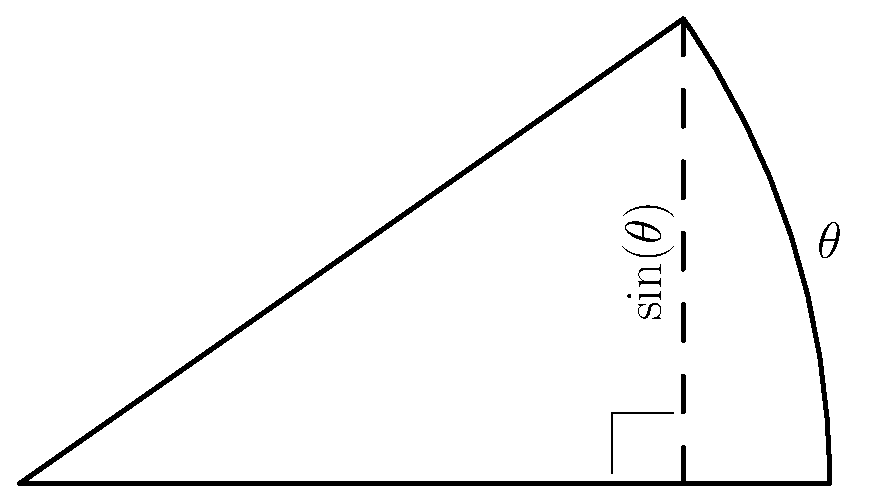
\includegraphics[width=0.3\textwidth]{ChapterGeom/Figures/GAI-smallAngle}
        \caption*{Small angle $\theta$ verusus $\sin(\theta).$}
\end{wrapfigure}

 Consider the following limit: $$ \lim_{x\rightarrow 0}\frac{\sin(\theta)}{\theta}$$
It is indeterminate of the form $\frac{0}{0}$.  Thus it is valid to apply LHR. \begin{align*}
\lim_{x\rightarrow 0}\frac{\sin(\theta)}{\theta} &=\lim_{x\rightarrow 0}\frac{\left(\sin(\theta)\right)'}{\left(\theta\right)'} \\
&=\lim_{x\rightarrow 0}\frac{\cos(\theta)}{1} \\
&=1
\end{align*}
    
    
\end{example}
\begin{exercise}{Interpreting the Above Example \Coffeecup}
Since the ratio of $\sin(\theta)$ to $\theta$ approaches 1 as $\theta$ gets small, it would be appropriate to say the following (fill in the blanks):
\begin{center}
\emph{For small values of $\theta$, \underline{\hspace{1in}}$\approx$\underline{\hspace{1in}}.}
\end{center}
    \solushun{
        \begin{center}
            \emph{For small values of $\theta$, \underline{$\sin(\theta)$}$\approx$\underline{$\theta$}.}
        \end{center}
    }{0in}
\end{exercise}
Note that this property comes up frequently in physics!  For example, when modeling the motion of a mass hanging from a spring, Hooke's Law tells us that force is proportional to displacement.  We use the same model to describe motion of a pendulum, even though in that case force is not technically proportional to displacement, but rather the \emph{sine} of displacement.  Why can we throw away the sine?  It is because for small displacements, the sine of the displacement is roughly equal to the displacement!
\begin{exercise}{Practice with LHR \Coffeecup \Coffeecup}
Evaluate the following limits using L'Hospital's Rule. In each case, justify why it is ok to use it!
\begin{itemize}
\item $ {\underset{x \rightarrow \infty}{\lim}}\hspace{.1in}\frac{x^2 }{ 2^x} $
\solushun{$${\lim_{x \rightarrow \infty}}\frac{x^2 }{ 2^x} = \frac{\infty}{\infty}$$Since we have the form $\frac{\infty}{\infty}$ we can use LHR.
$${\lim_{x \rightarrow \infty}}\frac{x^2 }{ 2^x}={\lim_{x \rightarrow \infty}}\frac{2x}{2^x\ln2}$$
Keep going:
$${\lim_{x \rightarrow \infty}}\frac{2x}{2^x\ln2}={\frac{1}{\ln2}\lim_{x \rightarrow \infty}}\frac{2}{2^x\ln2}={\frac{1}{(\ln2)^2}\lim_{x \rightarrow \infty}}\frac{1}{2^{x-1}}=0$$
}{1in}
\item $ {\underset{x \rightarrow 2}{\lim}}\hspace{.1in}\frac{x-2 }{ \sin(\pi x)} $
\solushun{
$${\lim_{x\to2}}\frac{x-2}{\sin(\pi x)}=\frac{0}{0}$$
So LHR is justified.
$${\lim_{x \to 2}}\frac{x-2}{\sin(\pi x)}={\lim_{x\to2}}\frac{\frac{\dif}{\dif x}(x-2)}{\frac{\dif}{\dif x}\sin(\pi x)}=\frac{1}{\pi\cos(\pi x)}=\frac{1}{\pi}$$
}{1in}
\item $ {\underset{x \rightarrow \infty}{\lim}}\hspace{.1in}\frac{ \arctan(x)-\pi/2 }{ \sin(1/x)} $
\solushun{$${\lim_{x\to\infty}}\frac{\arctan(x)-\pi/2}{\sin(1/x)}=\frac{0}{0}$$
So LHR is justified.
\begin{align*}
{\lim_{x\to\infty}}\frac{\arctan(x)-\pi/2}{\sin(1/x)}&={\lim_{x\to\infty}}\frac{\frac{\dif}{\dif x}(\arctan(x)-\pi/2)}{\frac{\dif}{\dif x}\sin(1/x)}={-\lim_{x\to\infty}}\frac{\frac{1}{x^2+1}}{\frac{1}
{x^2}\cos(1/x)}\\
&={-\lim_{x\to\infty}}\frac{x^2}{(x^2+1)\cos(1/x)}=-\frac{\infty}{\infty}\\
\text{One more time}\\
&={-\lim_{x\to\infty}}\frac{2x}{2x\cos(1/x)+\sin(1/x)+\frac{1}{x^2}\sin(1/x)}=-\frac{\infty}{\infty}\\
\text{And again}\\
&={-\lim_{x\to\infty}}\frac{2}{2\cos(\frac{1}{x})+2x(-\frac{1}{x^2}\sin(\frac{1}{x}))+\frac{1}{x^2}\cos(\frac{1}{x})-\frac{1}{x^4}\cos(\frac{1}{x})}\\
&=1
\end{align*}}{1in}
\end{itemize}
\AnswerKeyEntry{The limits are 0, $1/\pi$, and -1. }
\end{exercise}
\subsection{Other Indeterminate Forms}
There are many \LHR{other indeterminate forms} besides just $\frac{0}{0}$ and $\frac{\infty}{\infty}$.  Others that come up include: 
\begin{itemize}
\item $0\cdot \infty$
\item $0^0$
\item $1^\infty$
\item $\infty-\infty$
\end{itemize}
Often these other forms can be rearranged algebraically to become $\frac{0}{0}$ or $\frac{\infty}{\infty}$.  After this rearrangement, they can then be evaluated with LHR (or perhaps the algebra itself resolves the indeterminate form and LHR will not be needed).  Common helpful strategies include:

\begin{itemize}
\item Multiplying the top and bottom of the limit by the same expression (especially the conjugate of an expression involving a radical).
\item Taking $e$ to the $\ln$ of the limit.
\item Rewriting a product as a fraction via $a\cdot b = \frac{b}{\frac{1}{a}}$.
\end{itemize}
\begin{example}{Rewriting a Different Indeterminate Form}
 Consider the function $\sin(x)^{\tan(x)}$.  As $x$ approaches $\frac{\pi}{2}$ from the left, the function takes on the indeterminate form $1^\infty$.  Thus, we try the second strategy described above, where we take $e$ to the $\ln$ of the limit.  Proceeding:
 \begin{align*}
 \lim_{x\rightarrow \pi/2^-}\sin(x)^{\tan(x)}&= \lim_{x\rightarrow \pi/2^-}e^{\ln\left(\sin(x)^{\tan(x)}\right)}\\
 &=\lim_{x\rightarrow \pi/2^-}e^{\tan(x)\ln\left(\sin(x)\right)}\\
 \end{align*}
 
\begin{wrapfigure}{r}{0.3\textwidth}
 \begin{center}
 	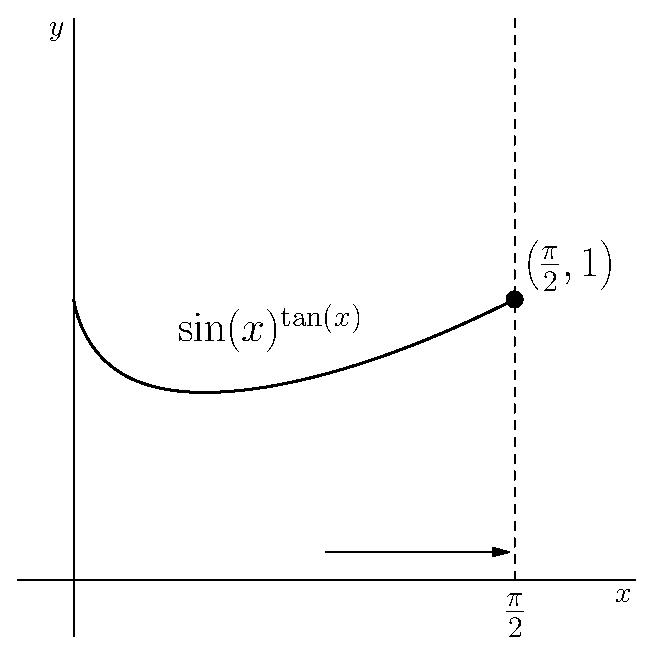
\includegraphics[width=0.3\textwidth]{ChapterGeom/Figures/LHR-SinetoTan}
 \end{center}
\end{wrapfigure}

Notice the exponent is now the indeterminate form $0\cdot\infty$.  Since the exponential function is continuous, we can move the limit inside and use LHR!
\begin{align*}
 \lim_{x\rightarrow \pi/2^-}\sin(x)^{\tan(x)}
 &=\lim_{x\rightarrow \pi/2^-}e^{\tan(x)\ln\left(\sin(x)\right)}\\
 &=e^{\lim_{x\rightarrow \pi/2^-}\left(\tan(x)\ln\left(\sin(x)\right)\right)}\\
 &=e^{\lim_{x\rightarrow \pi/2^-}\left(\frac{\ln\left(\sin(x)\right)}{\cot(x)}\right)}\\
 &=e^{\lim_{x\rightarrow \pi/2^-}\left(\frac{\left(\ln\left(\sin(x)\right)\right)'}{\left(\cot(x)\right)'}\right)}\\
 &=e^{\lim_{x\rightarrow \pi/2^-}\left(\frac{\frac{\cos(x)}{\sin(x)}}{-\csc^2(x)}\right)}\\
 &=e^{\lim_{x\rightarrow \pi/2^-}\left(-\cos(x)\sin(x)\right)}\\
 &=e^{-0\cdot 1}\\
 &=1
 \end{align*}
\end{example}
\begin{exercise}{Identifying LHR \Coffeecup}
In the example above, circle the exact step where LHR was applied.  Why was it ok to use LHR on that step?  Write a short sentence to explain.
\solushun{The steps from $e^{\lim_{x\rightarrow \pi/2^-}\left(\frac{\ln\left(\sin(x)\right)}{\cot(x)}\right)}$ to $e^{\lim_{x\rightarrow \pi/2^-}\left(\frac{\frac{\cos(x)}{\sin(x)}}{-\csc^2(x)}\right)}$. This was justified because $\lim_{x\to\pi/2^-}\ln(\sin(x))=\ln(1)=0$ and $\lim_{x\to\pi/2^-}\cot(x)=0$ also.\\}{0in}
\end{exercise}
\begin{exercise}{Rewriting \Coffeecup \Coffeecup \Coffeecup}
Utilize these strategies to rewrite the limits below as $\frac{0}{0}$ or $\frac{\infty}{\infty}$ and then evaluate.  Note that some of these may need LHR after rewriting and some may not!
\begin{itemize}
\item $  {\underset{x \rightarrow \infty}{\lim}}\hspace{.1in} x\cdot \sin (1/x) $
\solushun{\begin{align*}
\lim_{x\to\infty}x\cdot\sin(1/x)&=\lim_{x\to\infty}\frac{\sin (1/x)}{\frac{1}{x}}\\
&=\lim_{x\to\infty}\frac{\left(\sin (1/x)\right)'}{\left(\frac{1}{x}\right)'}\\
&=\lim_{x\to\infty}\frac{-\frac{1}{x^2}\cos(1/x)}{\frac{1}{x^2}}\\
&=\lim_{x\to\infty}\cos(1/x)=1
\end{align*}}{2in}
\item $  {\underset{x \rightarrow \infty}{\lim}}\hspace{.1in}  x - \sqrt{x^2+4x+3} $
\solushun{We actually don't need LHR for this one.
\begin{align*}
\lim_{x\to\infty}x-\sqrt{x^2+4x+3}&=\lim_{x\to\infty}\left(x-\sqrt{x^2+4x+3}\right)\cdot\frac{x+\sqrt{x^2+4x+3}}{x+\sqrt{x^2+4x+3}}\\
&=\lim_{x\to\infty}\frac{x^2-x^2-4x-3}{x+\sqrt{x^2+4x+3}}\\
&=\lim_{x\to\infty}\frac{-4x-3}{x+\sqrt{x^2+4x+3}}\\
&=\lim_{x\to\infty}\frac{-4-\frac{3}{x}}{1+\sqrt{1+\frac{4}{x}+\frac{3}{x^2}}}\\
&=\frac{-4}{1+\sqrt{1}}=\frac{-4}{2}=-2\\
\end{align*}}{2in}
\item $ \underset{x \rightarrow \infty}{\lim}\hspace{.1in}  \left(1+ \frac{1}{x} \right) ^x $ ({\bf Note: } This limit is often taken as the definition of the constant you get here!)
\solushun{Rewrite this as $e^{x\ln\left(1+\frac{1}{x}\right)}$
Then the limit can be moved into the exponent and resolved:
\begin{align*}
\lim_{x\to\infty}e^{x\ln\left(1+\frac{1}{x}\right)}=&e^{\lim_{x\to\infty}x\ln\left(1+\frac{1}{x}\right)}\\
=&e^{\lim_{x\to\infty}\frac{\ln\left(1+\frac{1}{x}\right)}{\frac{1}{x}}}\\
\text{Now apply LHR}\\
=&e^{\lim_{x\to\infty}\frac{\frac{1}{1+\frac{1}{x}}\cdot -x^{-2}}{-x^{-2}}}\\
=&e^{\lim_{x\to\infty}\frac{x}{x+1}}\\
\text{Apply LHR again}\\
=&e^{1}=e\\
\end{align*}}{2in}
\end{itemize}
\AnswerKeyEntry{The limits are $1$, $-2$, and $e$. }
\end{exercise}

\begin{exercise}{Polyexposaurus \Coffeecup \Coffeecup \Coffeecup}
\begin{itemize}
\item Any positive real number raised to the zero is...
\solushun{1\\}{.5in}
\item Zero raised to any positive real number is...
\solushun{0\\}{.5in}
\item So, what is $  {\underset{x \to 0^+}{\lim}}  x^x $? 
\solushun{\begin{align*}
\lim_{x\to0^+}x^x&=e^{\lim_{x\to0^+}x\ln x}\\
\lim_{x\to0^+}x^x&=e^{-\lim_{x\to0^+}\frac{\ln x}{\frac{1}{x}}}\tag{Goes to $\frac{-\infty}{\infty}$ so we factor out $-1$}\\
\lim_{x\to0^+}x^x&=e^{-\lim_{x\to0^+}\frac{\frac{1}{x}}{-\frac{1}{x^2}}}\\
\lim_{x\to0^+}x^x&=e^{\lim_{x\to0^+}x}\\
\lim_{x\to0^+}x^x&=e^{0}=1\\
\end{align*}}{2in}
\end{itemize}
\AnswerKeyEntry{The results are 1, 0, and 1.}
\end{exercise}

Be careful when using LHR to only apply it in the two indeterminate forms specified above.  Applying LHR to an expression that is not either $\frac{0}{0}$ or $\frac{\infty}{\infty}$ will most likely produce incorrect results.  

\begin{exercise}{L'Urgent Care \Coffeecup \Coffeecup }
Consider the following limit.
$$ {\lim_{x \to \pi }}  \frac{\sin(x)}{x} $$
\begin{itemize}
\item Why would it be wrong to apply LHR to the above limit?
\solushun{The denominator does not approach 0\\}{.5in}
\item  What do you get if you blindly apply LHR?
\solushun{$$\lim_{x\to\pi}\cos(x)=1$$}{.5in}
\item  What should the limit actually be?
\solushun{$$\lim_{x\to\pi}\sin(x)\cdot\frac{1}{x}=0\cdot\frac{1}{\pi}=0$$}{.5in}
\end{itemize}
\end{exercise}

\subsection{Growth Orders}\label{tomato} 

\growthorder{LHR} is often used for comparing \LHR{growth orders} of functions.  To compare the growth orders of functions, we take the limit of their ratio as $x$ approaches infinity and then see if the ratio approaches zero, a nonzero constant, or infinity to see which is growing faster.  More formally:

\begin{definition}{Growth Order}\label{tomahto}

Let $f(x)$ and $g(x)$ be functions on the real numbers. 
\begin{itemize}
\item If $\lim_{x\rightarrow \infty}\frac{f(x)}{g(x)}=0$, then $g(x)$ has \emph{larger growth order} than $f(x)$. 
\item If $\lim_{x\rightarrow \infty}\frac{f(x)}{g(x)}$ is a nonzero constant, then $f(x)$ and $g(x)$ have the \emph{same growth order}. 
\item If $\lim_{x\rightarrow \infty}\frac{f(x)}{g(x)}=\infty$, then $f(x)$ has \emph{larger growth order} than $g(x)$. 
\end{itemize}
\end{definition}
\begin{exercise}{Comparing the Growth Orders of Two Lines \Coffeecup \Coffeecup}
Consider the following two linear functions: \begin{align*}
f(x)&=6x+1\\
g(x)&=2x-1
\end{align*}
Fill out the table below to study some of their values and corresponding ratios.  Use decimal approximations for values that aren't integers.  \begin{center}
\begin{tabular}{|c||c|c|c|c|c|} \hline
$x$ & 1 & 10 & 100 & 1,000 & 10,000 \\ \hline
& & & & & \\
$f(x)$ & & & & & \\
& & & & & \\
$g(x)$ & & & & & \\
& & & & & \\
$f(x)/g(x) $ & & & & & \\
& & & & & \\ \hline
\end{tabular}
\end{center}
\solushun{ \begin{center}
\begin{tabular}{|c||c|c|c|c|c|} \hline
$x$ & 1 & 10 & 100 & 1,000 & 10,000 \\ \hline
& & & & & \\
$f(x)$ & 7& 61& 601& 6001& 60001\\
& & & & & \\
$g(x)$ & 1& 19& 199& 1999& 19999\\
& & & & & \\
$f(x)/g(x)$ & 7& 3.2105& 3.0201& 3.0020& 3.0002\\
& & & & & \\ \hline
\end{tabular}
\end{center}}{0in}
\begin{itemize}
\item From the table, does it appear that the ratio $f(x)/g(x)$ is approaching zero, infinity, or a nonzero constant?
\solushun{It appears that the ratio approaches the constant 3.\\}{.3in}
\item Use LHR to compute the limit $$\lim_{x\rightarrow \infty}\frac{f(x)}{g(x)} $$
How does it relate to the values in the data table? 
\solushun{\begin{align*}
\lim_{x\to\infty}\frac{f(x)}{g(x)} &=\frac{\infty}{\infty}\\
&=\lim_{x\to\infty}\frac{f'(x)}{g'(x)}\\
&=\lim_{x\to\infty}\frac{6}{2}=3
\end{align*}
It is the ratio of the leading coefficients.\\}{.3in}
\item See the above definition of Growth Order.  In this case, would you say $f$ and $g$ have the same growth order, or does one function have larger growth order than the other?
\solushun{Since 3 is a nonzero constant, the two have the same growth order.}{.3in}
\end{itemize}
\AnswerKeyEntry{Their ratio converges to 3 (both numerically in the table, and analytically as evaluated by LHR).  Since this is a nonzero constant, the two functions have the same growth order.}
\end{exercise}

The above calculation justifies why it is ok to talk about something having \emph{linear growth order} or \emph{growing linearly}.  Any two lines have the same growth order (ignoring vertical and horizontal), so it is perfectly well-defined to talk about linear growth even if the slope or intercepts of the lines being discussed are unknown.  

This concept comes up frequently in computer science when you try to measure the runtime of algorithms.  If $f(x)$ is the number of operations performed by an algorithm that is handed an input of size $x$, then a logarithmic growth order of $f(x)$ is generally more desirable than a linear growth order, which is more desirable than quadratic growth order, and so on.

\begin{exercise}{A Visual Representation of Growth Order \Coffeecup \Coffeecup \Coffeecup}

In each of the graphs below, there is a graph of $f(x)$ and a graph of $g(x)$.  Based on the graphs, do you expect that $f$ and $g$ have the same growth order, or is one larger?

\begin{tabular}{l c }
1. & \raisebox{\dimexpr-\height + 1.5ex\relax}{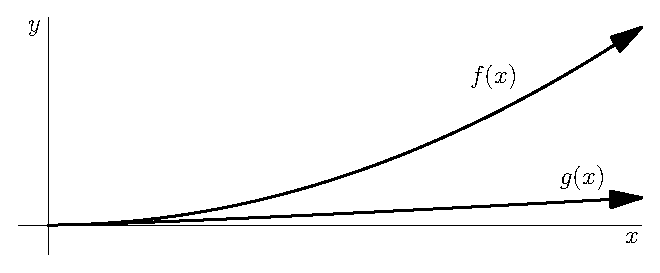
\includegraphics[width=250pt]{ChapterGeom/Figures/Prob1.eps}} \\
2. & \raisebox{\dimexpr-\height + 1.5ex\relax}{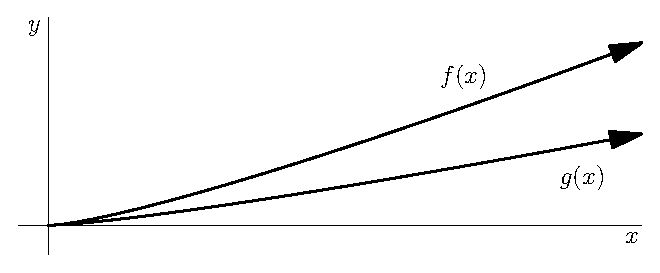
\includegraphics[width=250pt]{ChapterGeom/Figures/Prob2.eps}} \\
3. & \raisebox{\dimexpr-\height + 1.5ex\relax}{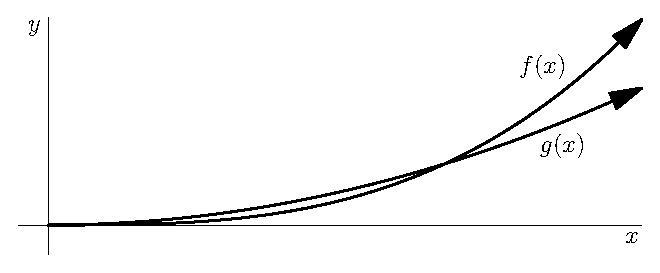
\includegraphics[width=250pt]{ChapterGeom/Figures/Prob3.eps}}
\end{tabular}

\solushun{
    \begin{enumerate}
        \item The ratio between $f$ and $g$ seems to be growing, so $f$ has a larger growth order.
        \item The ratio between $f$ and $g$ seems to be consistently about 2, so they have the same growth order.
        \item The ratio between $f$ and $g$ seems to be growing, so $f$ has a larger growth order.
    \end{enumerate}
}{0in}

\AnswerKeyEntry{In the first and third, the ratio between $f$ and $g$ seems to grow without bound, so $f$ has larger growth order.  In the second, the ratio of $f$ to $g$ seems to always be right around 2.  Thus, they have the same growth order.}
\end{exercise}

\begin{example}{Logarithmic Growth Order}
\begin{wrapfigure}{r}{0.5\textwidth}
 \begin{center}
 	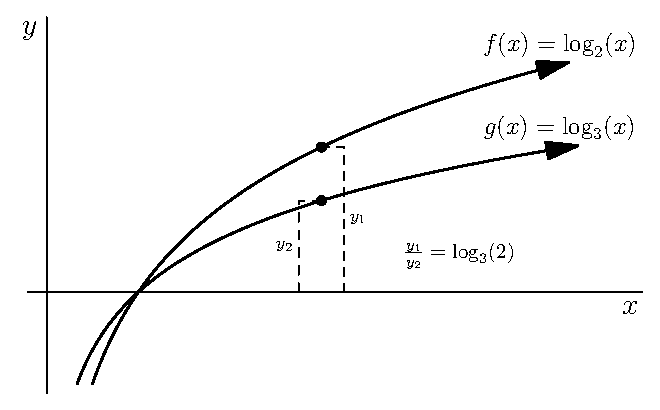
\includegraphics[width=0.5\textwidth]{ChapterGeom/Figures/LogGrowthOrder}
 \end{center}
\end{wrapfigure}
Here we compare the growth orders of the following logarithmic functions:
\begin{align*}
f(x)&=\log_2(x) \\
g(x)&=\log_3(x)
\end{align*}
Definition \ref{tomato}.\ref{tomahto}. shows that we should take the limit of their ratio and then see if we get zero, infinity, or a nonzero constant.

\begin{align*}
\lim_{x\to \infty}\frac{f(x)}{g(x)}&=\lim_{x\to \infty}\frac{\log_2(x)}{\log_3(x)}\\
&=\lim_{x\to \infty}\log_3(2) \\
&=\log_3(2)
\end{align*}
Since their ratio came out to a nonzero constant, we conclude that those two functions in fact have the same growth order (even though  the $y$-coordinate of $f(x)$ is always bigger).  By a similar calculation, we could observe that in fact any two logarithms have the same growth order regardless of what the base is!
\end{example}

\begin{exercise}{Race of the Turtles \Coffeecup \Coffeecup}
Rank the following functions by growth order from slowest to fastest by comparing their growth orders two at a time:
\begin{align*}
f(x)&=x {\ln} (x) \\
g(x)&=x^{1.1} \\
h(x)&=x\left( {\ln} (x) \right)^2
\end{align*}

\solushun{
Comparing $f(x)$ with $g(x)$:
\begin{align*}
\lim_{x\to\infty}\frac{x\ln(x)}{x^{1.1}}&=\lim_{x\to\infty}\frac{\ln(x)}{x^{0.1}}\\
&=\lim_{x\to\infty}\frac{x^{-1}}{0.1x^{-0.9}}\tag{By LHR}\\
&=\lim_{x\to\infty}\frac{x^{-0.1}}{0.1}=0
\end{align*}
So $g(x)$ has greater growth order than $f(x)$. Comparing $f(x)$ and $h(x)$:
\begin{align*}
\lim_{x\to\infty}\frac{x\ln(x)}{x\left(\ln(x)\right)^2}=\lim_{x\to\infty}\frac{1}{\ln(x)}=0
\end{align*}
So $h(x)$ has greater growth order than $f(x)$. Comparing $g(x)$ and $h(x)$:
\begin{align*}
\lim_{x\to\infty}\frac{x^{1.1}}{x\left(\ln(x)\right)^2}&=\lim_{x\to\infty}\frac{x^{0.1}}{\left(\ln(x)\right)^2}\\
&=\lim_{x\to\infty}\frac{0.1x^{-0.9}}{2\ln(x)x^{-1}}\tag{By LHR}\\
&=\frac{1}{20}\lim_{x\to\infty}\frac{x^{0.1}}{\ln(x)}\\
&=\frac{1}{20}\lim_{x\to\infty}\frac{0.1x^{-0.9}}{x^{-1}}\tag{By LHR again}\\
&=\lim_{x\to\infty}x^{0.1}=\infty
\end{align*}
So $g(x)$ has higher growth order than $h(x)$.
Then, the overall ranking is: $f(x),h(x),g(x)$.\\
}{2in}

\end{exercise}

\begin{exercise}{Exponential vs Polynomial \Coffeecup \Coffeecup \Coffeecup }
Explain why an exponential function will always have larger growth order than an polynomial function. 
\solushun{An exponential function $c^x$ will always have a larger growth order than any polynomial function because the derivative will always contain another $c^x$ term. That is $(c^x)'=c^x\ln(c)$. In the simplest case, $(e^x)'=e^x$. Thus, as long as $x>0$, the limit of any of the derivatives of an exponential function, $\lim_{x\to\infty}(c^x)^{(k)}$, with $k>0$ is always $\infty$.

A polynomial, on the other hand, either has derivatives that eventually become constant (if the power $n$ of a term $x^n$ is greater than 0), or which become successively smaller (if $n$ is less than 0). Thus, the polynomial's successive derivatives will eventually become less than that of an exponential function.\\

On the other hand, if $x<0$, the exponential function will always have a smaller growth order than any polynomial.\\}{2in}
\end{exercise}

%
\section{Improper Integrals} In Calculus I,  all of our definite integrals corresponded to the area of a bounded region.  A definite integral over an \area{unbounded region} is called \emph{\integ{improper}}.
\subsection{Vertically Unbounded Regions}\label{VertUnbounded}
If the integrand has a vertical asymptote between the limits of integration, we must proceed by approximating the unbounded region with a bounded region and then taking a limit.  

\begin{exercise}{Analyzing a Vertical Asymptote \Coffeecup \Coffeecup}\label{LogArea}

Consider the following integral: $$\int_0^1 \ln(x) \dif x $$

\begin{itemize}
\item Explain why the above integral would be called improper. 

\solushun{$\ln(x)$ has a vertical asymptote at $x=0$.\\}{1in}

\item Find the antiderivative of the function $\ln(x)$.

\solushun{Using IBP, we let $u=\ln(x), \dif u = \frac{1}{x}, v=x, \dif v = \dif x$.
\begin{align*}
\int\ln(x)\dif x = x\ln(x)-\int\dif x=x\ln(x)-x+C
\end{align*}}{1in}

\item Fill out the following table.  For each definite integral, include a rough sketch of the region whose signed area it corresponds to.  

\begin{center}
\begin{tabular}{|c|c|c|} \hline
 & & \\
\hspace{.2in} $c$ \hspace{.2in} & \hspace{.2in} $\int_c^1 \ln(x) \dif x $ \hspace{.2in} & \hspace{.4in} Graph of Region \hspace{.4in} \\
 & & \\ \hline \hline
 & & \\
0.1 & & \\
 & & \\ \hline
  & & \\
0.01 & & \\
 & & \\ \hline
 & & \\
0.001 & & \\
 & & \\ \hline
  & & \\
0.0001 & & \\
 & & \\ \hline
\end{tabular}
\end{center}

\solushun{\begin{center}
\begin{tabular}{|c|c|c|} \hline
 & & \\
\hspace{.2in} $c$ \hspace{.2in} & \hspace{.2in} $\int_c^1 \ln(x) \dif x $ \hspace{.2in} & \hspace{.4in} Graph of Region \hspace{.4in} \\
 & & \\ \hline \hline
 & & \\
0.1 & -0.6697 & 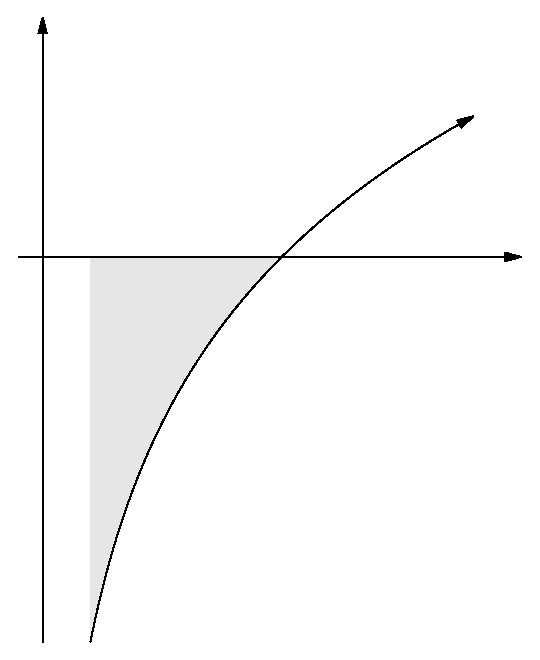
\includegraphics[width=100pt]{ChapterGeom/Figures/ln_2.eps} \\
 & & \\ \hline
  & & \\
0.01 & -0.9349& 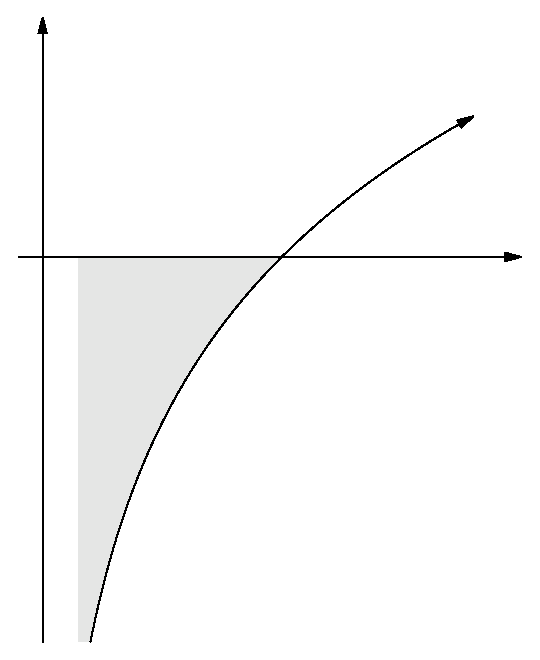
\includegraphics[width=100pt]{ChapterGeom/Figures/ln_3.eps}\\
 & & \\ \hline
 & & \\
0.001 & -0.9921 & 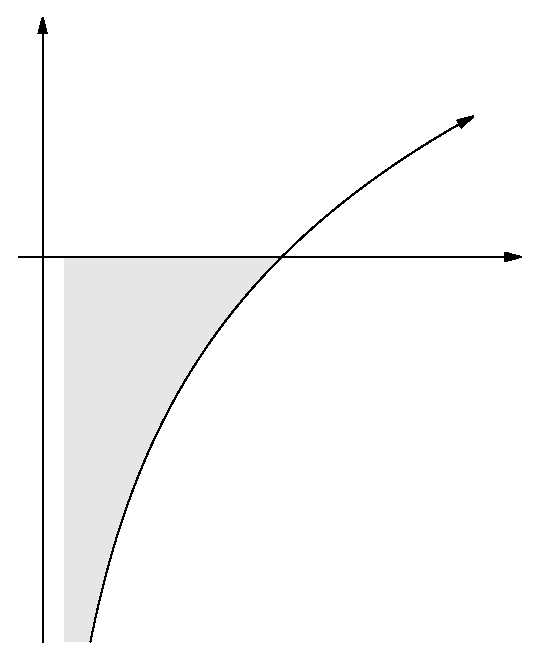
\includegraphics[width=100pt]{ChapterGeom/Figures/ln_4.eps}\\
 & & \\ \hline
  & & \\
0.0001 & -0.9989 &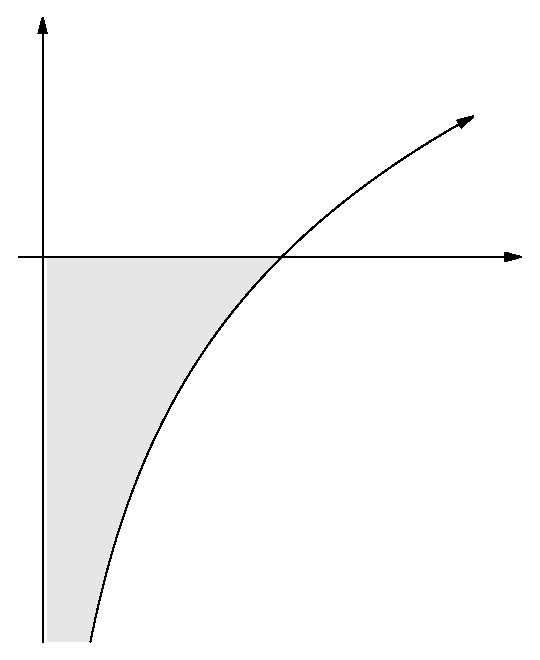
\includegraphics[width=100pt]{ChapterGeom/Figures/ln_5.eps} \\
 & & \\ \hline
\end{tabular}
\end{center}
}{0in}

\item As $c$ approaches 0 from the right, what does the area seem to be approaching?

\solushun{It seems to be approaching -1\\}{1in}
\end{itemize}
\end{exercise}

The above calculation motivates the definition of an improper integral.

\FormulaBox{Definition of Improper Integral I}{
\begin{tabular}{c}

If $f(x)$ has a vertical asymptote at $x=a$ \\ but is continuous on the interval $\left(a,b\right]$, \\
then the improper integral is defined as \\ $\int_a^b f(x) \dif x = \lim_{c\rightarrow a^+} \int_c^b f(x) \dif x $

\end{tabular}
}

If this limit converges to a number, then we say the \conv{improper integral} \emph{converges}.  Otherwise, we say the \divergence{improper integral} \emph{diverges}.
 We apply the definition to finish off the above exercise.

\begin{example}{Area Between the Axes and Natural Log}
To calculate the area between $y=0$, $x=0$, and $y=\ln(x)$, we use the definition of improper integral.  We proceed with the following calculation: 
\begin{align*}
\int_0^1 \ln(x) \dif x &= \lim_{c\rightarrow 0^+} \int_c^1 \ln(x) \dif x \\
&=\lim_{c\rightarrow 0^+}  \left. x\ln(x)-x \right]_{x=c}^{x=1} \\
&=\lim_{c\rightarrow 0^+}  \left(1\ln(1)-1\right) -\left(c\ln(c)-c\right)
\end{align*}

In the above limit, all terms are harmless except for $\lim_{c\rightarrow 0}c\ln(c)$, which is indeterminate of the form $0\cdot \infty$.  We can rewrite as $$\lim_{c\rightarrow 0^+}c\ln(c)=\lim_{c\rightarrow 0^+}\frac{\ln(c)}{\left(\frac{1}{c}\right)}$$ to get it in the form $\frac{\infty}{\infty}$ (up to a minus sign which is harmless), where we can apply LHR.
\end{example}

\begin{exercise}{We'll Actually Finish This Problem Here, Promise \Coffeecup \Coffeecup}
Finish evaluating the limit above and verify the area matches your estimations from Exercise \ref{VertUnbounded}.\ref{LogArea}.
\solushun{\begin{align*}
\lim_{c\to0^+}\frac{\ln(c)}{\frac{1}{c}}&=\lim_{c\to0^+}\frac{\frac{1}{c}}{-1\frac{1}{c^2}}\tag{By LHR}\\
&=\lim_{c\to0^+}-c=0
\end{align*}
Then, we can evaluate the original integral:
$$\lim_{c\rightarrow 0^+}  \left(1\ln(1)-1\right) -\left(c\ln(c)-c\right)=(1\cdot0-1)-0=-1$$
}{1in}
\end{exercise}

Let us now construct the analogous definition for a vertical asymptote occurring at the right-hand endpoint rather than the left-hand endpoint.

\begin{exercise}{Completing the Definition \Coffeecup \Coffeecup \Coffeecup}

Suppose a function $f(x)$ is continuous on $[a,b)$ but had a vertical asymptote at $x=b$.  Use the diagram below to help complete the definition of such an improper integral.  Fill in the boxes below.

\FormulaBox{Definition of Improper Integral II}{
\begin{tabular}{c}

If $f(x)$ has a vertical asymptote at $x=a$ \\ but is continuous on the interval $\left(a,b\right]$, \\
then the improper integral is defined as \\ $\int_a^b f(x) \dif x = \lim_{c\rightarrow \square } \int_\square^\square f(x) \dif x $

\end{tabular}
}
\begin{center}
    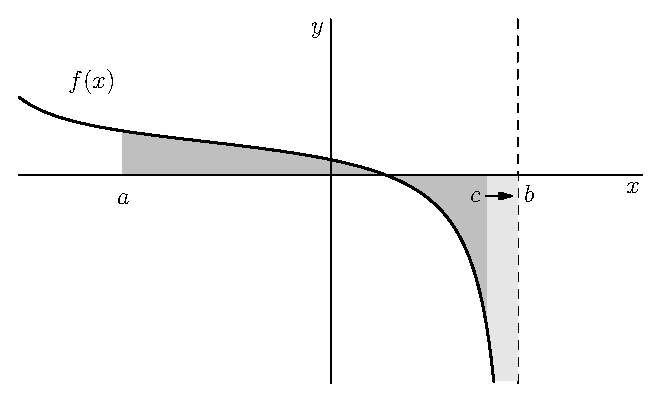
\includegraphics[width=300pt]{ChapterGeom/Figures/abcint.eps}
\end{center}
Once again, if this limit converges to a number, then we say the \conv{improper integral} \emph{converges}.  Otherwise, we say the \divergence{improper integral} \emph{diverges}.
\end{exercise}

\begin{exercise}{Illustrate the Computation  \Coffeecup} Here we demonstrate an example of computing an improper integral with the vertical asymptote at the right-hand endpoint.  Illustrate the computation on the axes below.  Show the graph of the integrand and the locations of the bounds $a,b,$ and $c$.  

\begin{align*}
\int_{x=0}^{x=\pi/2}\tan(x)\dif x &= \lim_{c\rightarrow \pi/2^-}\int_{x=0}^{x=c}\tan(x)\dif x \\
&=\lim_{c\rightarrow \pi/2^-}\left. -\ln\left(\cos(x)\right)\right]_{x=0}^{x=c} \\
&=\lim_{c\rightarrow \pi/2^-} -\ln\left(\cos\left(c\right)\right)+\ln\left(\cos(0)\right) \\
&=\infty
\end{align*}
\begin{center}
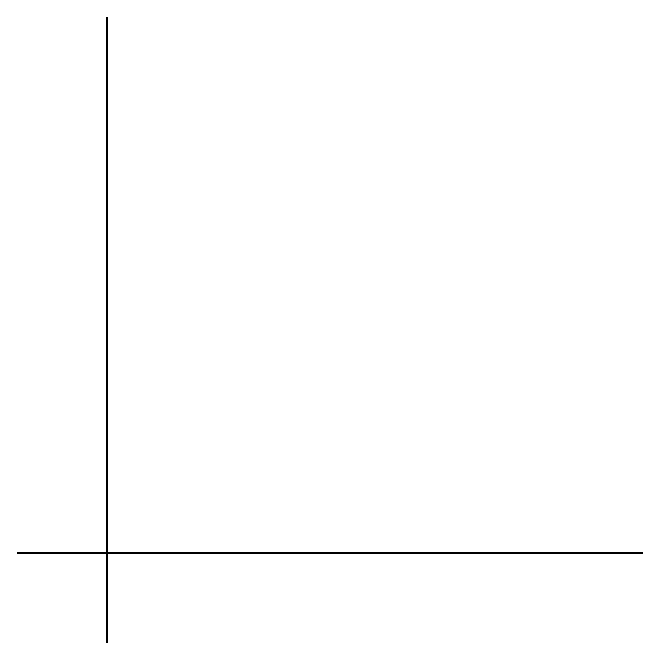
\includegraphics[scale=0.8]{quad1.eps}
\end{center}
\solushun{\begin{center}
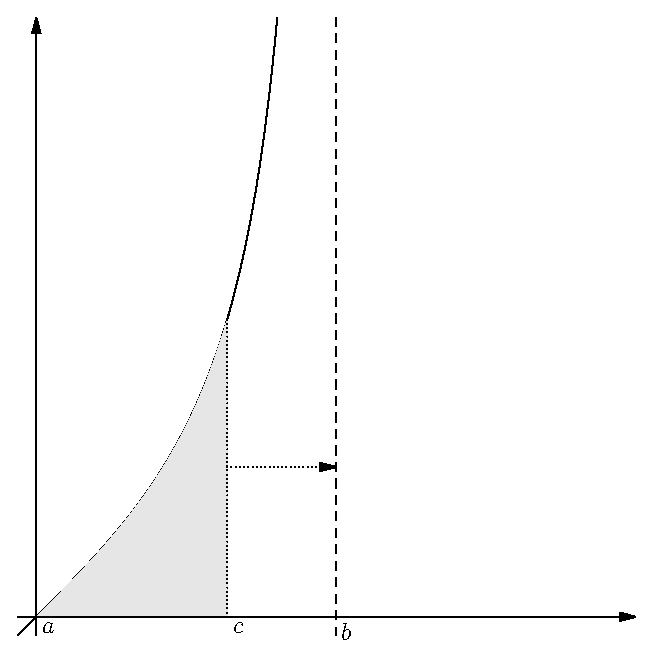
\includegraphics[scale=0.8]{ChapterGeom/Figures/tanintsolushun.eps}
\end{center}
}{0in}
\end{exercise}

If the vertical asymptote is in the interior (rather than at an endpoint) of the interval over which you are integrating, it may be necessary to split it into several integrals.

\begin{example}{A Particular Unbounded Region }
Suppose we wish to calculate the area bounded by the $x$-axis, the line $x=1$, the line $x=-1$, and the graph of $f(x)=\frac{1}{\sqrt{|x|}}$.  Notice the function has a vertical asymptote at $x=0$, which is in the interior of the interval over which we wish to integrate.  Thus, we split the integral into two integrals.  The first has a vertical asymptote at the right-hand endpoint and the second has a vertical asymptote at the left-hand endpoint.  We handle each accordingly.

\begin{align*}
\int_{-1}^{1} \frac{1}{\sqrt{|x|}}\dif x&=\int_{-1}^{0} \frac{1}{\sqrt{|x|}}\dif x+\int_{0}^{1} \frac{1}{\sqrt{|x|}}\dif x \\ 
&=\lim_{c_1 \rightarrow 0^-} \int_{-1}^{c_1} \frac{1}{\sqrt{|x|}} \dif x + \lim_{c_2 \rightarrow 0^+} \int_{c_2}^1 \frac{1}{\sqrt{|x|}} \dif x 
\end{align*} 

We now evaluate each of those integrals separately and add their totals.
\begin{align*}
\lim_{c_1 \rightarrow 0^-} \int_{-1}^{c_1} \frac{1}{\sqrt{|x|}} \dif x &=\lim_{c_1 \rightarrow 0^-} \left. {-2\sqrt{|x|}}\right|_{x=-1}^{x=c_1} \\
&=\lim_{c_1 \rightarrow 0^-}  {-2\sqrt{-c_1}}+2\sqrt{1} \\
&=0+2 \\
&=2
\end{align*}
The other region is just a reflection across the $y$-axis and thus must also have area 2. We conclude $$ \int_{-1}^{1} \frac{1}{\sqrt{|x|}}\dif x=4 $$

	\begin{center}       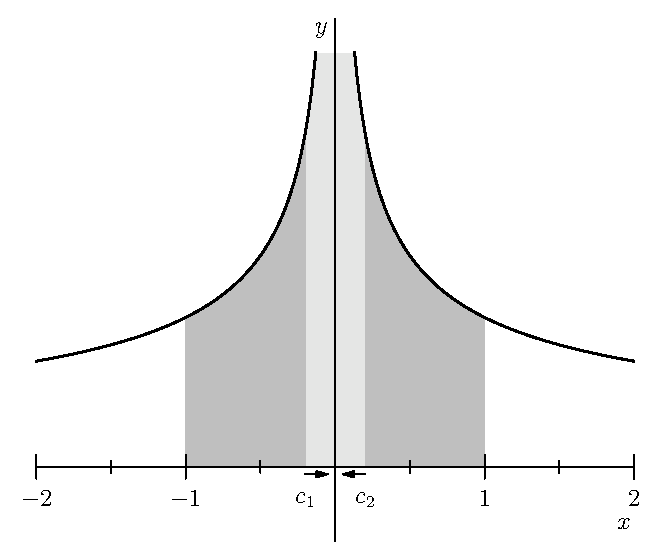
\includegraphics[width=300pt]{ChapterGeom/Figures/onesqrtx.eps}
    \end{center}
 \end{example}
 
\begin{exercise}{Some Subtle Sign Business \Coffeecup}
In the above computation, why is there a negative sign on the antiderivative, producing $-2\sqrt{|x|}$ instead of just $2\sqrt{|x|}$?  ({\bf Hint:} Graph the function $2\sqrt{|x|}$!)
\solushun{In order to evaluate the integral of an absolute value function, we treat it as a piecewise function. So:
$$\int\frac{1}{\sqrt{|x|}}\dif x=\int\frac{1}{\sqrt{-x}}\dif x=\int(-x)^{-\frac{1}{2}}\dif x=-2\sqrt{-x}$$ Since $-x=|x|$ when $x<0$, we can write $-2\sqrt{|x|}$.
}{1in}
\end{exercise}

Ok, now you give it a shot!  
\begin{exercise}{Improper Integral Practice \Coffeecup \Coffeecup}
Evaluate the following integrals and draw graphs similar to the figure above.  Show how you are evaluating the improper integral as a limit of integrals of bounded regions.
\begin{itemize}
\item $\int_{2}^4\frac{1}{\sqrt{x-2}}\dif x $

\solushun{\begin{align*}
\int_{2}^4\frac{1}{\sqrt{x-2}}\dif x &=\lim_{c\to2^+}\int_{c}^4\frac{1}{\sqrt{x-2}}\dif x\\
&=\lim_{c\to2^+}\left.2\sqrt{x-2}\right|^4_c\\
&=\lim_{c\to2^+}2\sqrt{2}-2\sqrt{c-2}=2\sqrt{2}
\end{align*}}{2in}

\item $ \int_{2}^4 \frac{1}{x^2-4}\dif x $

\solushun{
\begin{align*}
\int_{2}^4 \frac{1}{x^2-4}\dif x&=\lim_{c\to2^+}\int_{x=c}^{x=4}\frac{1}{x^2-4}\dif x\\
&=\lim_{c\to2^+}\frac{1}{4}\int_{x=c}^{x=4}\frac{1}{x-2}-\frac{1}{x+2}\dif x\tag{Via PFD}\\
&=\lim_{c\to2^+}\frac{1}{4}\left[\ln\left|x-2\right|-\ln\left|x+2\right|\right]^4_c\\
&=\lim_{c\to2^+}\frac{1}{4}\left[\ln\left|\frac{x-2}{x+2}\right|\right]^4_c\\
&=\lim_{c\to2^+}\frac{1}{4}\left[\ln\left|\frac{2}{6}\right|-\ln\left|\frac{c-2}{c+2}\right|\right]\\
&=\lim_{c\to2^+}\frac{1}{4}\left[\ln\left|\frac{2}{6}\right|-(-\infty)\right]=\infty\\
\end{align*}}{2in}

\item $ \int_{0}^{\pi /2} \sec(x) \dif x $
\solushun{
\begin{align*}
\int_{0}^{\pi /2} \sec(x) \dif x &=\lim_{c\to\frac{\pi}{2}^-}\int_{0}^{c} \sec(x) \dif x\\
&=\lim_{c\to\frac{\pi}{2}^-}\ln\left|\sec(x)+\tan(x)\right|^c_0\\
&=\lim_{c\to\frac{\pi}{2}^-}\ln\left|\sec(c)+\tan(c)\right|-\ln\left|\sec(0)+\tan(0)\right|\\
&=\ln\left|\infty+\infty\right|-\ln\left|1\right|=\infty\\
\end{align*}}{2in}
\item $ \int_{-\pi/2}^{\pi /2} \csc^2(x) \dif x $

\solushun{
\begin{align*}
\int_{-\pi/2}^{\pi /2} \csc^2(x) \dif x&=\lim_{c_1\to0^-}\int_{-\pi/2}^{c_1} \csc^2(x) \dif x+\lim_{c_2\to0^+}\int_{c_2}^{\pi/2} \csc^2(x) \dif x
\end{align*}
Since the function is symmetric, we can start with just the left side.
\begin{align*}
\lim_{c\to0^-}\int_{-\pi/2}^{c} \csc^2(x) \dif x&=\lim_{c\to0^-}\left[\cot(x)\right]^c_{-\pi/2}\\
&=\lim_{c\to0^-}\cot(c)-\cot(-\pi/2)=\infty-0=\infty\\
\end{align*}
Since the function is symmetric, we can double the result, which is the same.}{2in}

\end{itemize}
\AnswerKeyEntry{The integrals evaluate to $2\sqrt{2},\infty,\infty,$ and $\infty$.}
\end{exercise}

\subsection{Horizontally Unbounded Regions}

If the integral is over an interval that includes plus or minus infinity as one of the endpoints, we must proceed by approximating via a bounded interval and then taking the limit as the endpoint goes to plus or minus infinity.

\FormulaBox{Definition of Improper Integral III}{\begin{tabular}{c}
Let $f(x)$ be continuous on the interval $\left[a,\infty\right)$ for some real number $a$. \\ Then we define
$ \int_{a}^\infty f(x)\dif x = \lim_{c \rightarrow \infty} \int_{a}^c f(x)\dif x. $ 
\end{tabular}}
An integral to negative infinity is defined analogously via the corresponding limit. 

\begin{exercise}{Finding $c$ \Coffeecup}
	\begin{center}
        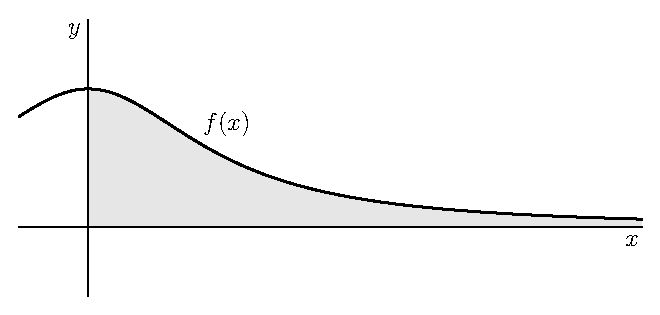
\includegraphics[width=300pt]{ChapterGeom/Figures/unboundhorizont.eps}
	\end{center}
Here is a graph that represents the above definition for $a=0$.  Interpret the definition by labeling $c$ on the graph and explaining the role it plays.  \vspace*{1in}
\end{exercise}

\begin{example}{Area Under $f(x)=\frac{1}{x^2}$}

	\begin{wrapfigure}{r}{0.3\textwidth}
    	\centering
		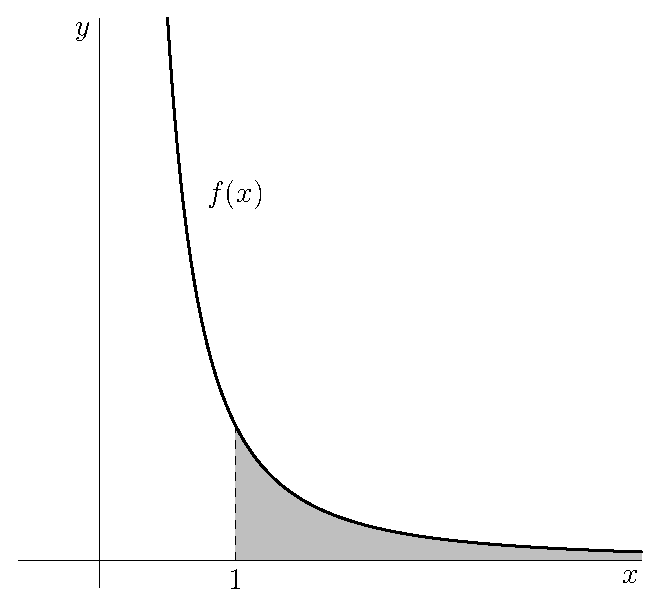
\includegraphics[width=0.3\textwidth]{ChapterGeom/Figures/AreaUnder1Overx2}
	\end{wrapfigure}

Suppose we wish to compute the area under the curve $f(x)=\frac{1}{x^2}$ over the interval $\left[1,\infty\right)$.  We apply the definition of the improper integral as a limit of bounded integrals.  

\begin{align*}
\int_{x=1}^{x=\infty}\frac{1}{x^2}\dif x &= \lim_{c \rightarrow \infty} \int_{x=1}^{x=c} \frac{1}{x^2} \dif x \\
&= \lim_{c \rightarrow \infty} \left.-\frac{1}{x} \right]_{x=1}^{x=c}\\
&= \lim_{c \rightarrow \infty} -\frac{1}{c}+\frac{1}{1} \\
&=1
\end{align*}
Thus, the area under the curve is 1.
\end{example}

\begin{exercise}{Area Under $1/x^p$ \Coffeecup \Coffeecup \Coffeecup}
\begin{itemize}
\item Calculate the improper integral $\int_{x=1}^{x=\infty}\frac{1}{x^3}\dif x$.

\solushun{
\begin{align*}
\int_{x=1}^{x=\infty}\frac{1}{x^3}\dif x&=\lim_{c\to\infty}\int_{x=1}^{x=c}\frac{1}{x^3}\dif x\\
&=\lim_{c\to\infty}\left.-\frac{1}{2x^2}\right|_{x=1}^{x=c}\\
&=\lim_{c\to\infty}-\frac{1}{2c^2}+\frac{1}{2(1)^2}=\frac{1}{2}
\end{align*}
}{1in}

\item Calculate the improper integral $\int_{x=1}^{x=\infty}\frac{1}{x^{1}}\dif x$.

\solushun{
\begin{align*}
\int_{x=1}^{x=\infty}\frac{1}{x^{1}}\dif x&=\lim_{c\to\infty}\int_{x=1}^{x=c}\frac{1}{x^{1}}\dif x\\
&=\lim_{c\to\infty}\ln(x)|^{x=c}_{x=1}\\
&=\lim_{c\to\infty}\ln(c)-\ln(1)=\infty-0=\infty
\end{align*}}{1in}

\item Calculate the improper integral $\int_{x=1}^{x=\infty}\frac{1}{x^{1/2}}\dif x$.
\solushun{
\begin{align*}
\int_{x=1}^{x=\infty}\frac{1}{x^{1/2}}\dif x&=\lim_{c\to\infty}\int_{x=1}^{x=c}\frac{1}{x^{1/2}}\dif x\\
&=\lim_{c\to\infty}\left.2x^{\frac{1}{2}}\right|_{x=1}^{x=c}\\
&=\lim_{c\to\infty}2c^{\frac{1}{2}}-2(1)^{\frac{1}{2}}\\
&=\infty-2=\infty
\end{align*}}{1in}
\item For what real numbers $p$ will $\int_{x=1}^{x=\infty}\frac{1}{x^{p}}\dif x$ converge?  For what $p$ will it diverge?
\solushun{For $p>1$, the $\int_{x=1}^{x=\infty}\frac{1}{x^{p}}\dif x$ will converge because the antiderivative of $x^{-p}, p>1$ will not transform the function into one with positive growth order (a positive exponent). However, the antiderivative of any function $x^{-p}, p\leq1$ will have a positive exponent and thus will diverge.\\}{1in}
\end{itemize}
\end{exercise}

If the integral is across the entire real number line, one must split into two separate integrals, similar to how we handled a vertical asymptote in the interior of our interval.  


\FormulaBox{Definition of Improper Integral III}{\begin{tabular}{c}
Let $f(x)$ be continuous on the entire real number line. \\ For any real number $a$, we define 
$ \int_{-\infty}^\infty f(x)\dif x = \int_{-\infty}^a f(x)\dif x + \int_{a}^\infty f(x)\dif x.$ 
\end{tabular}}

For the following problems, you may spot yourself the following fact we will prove in Calc 3: $$ \int_{-\infty}^\infty e^{-x^2}\dif x = \sqrt{\pi}$$

\begin{exercise}{More Practice with Improper Integrals \Coffeecup \Coffeecup}

Now, try the following integrals and for each draw a graph like the above figure that represents your integral as a limit of integrals of bounded regions.  Also, for the following problems, you may spot yourself the following fact we will prove in Calc 3: $$ \int_{-\infty}^\infty e^{-x^2}\dif x = \sqrt{\pi}$$


\begin{itemize}
\item $ \int_{0}^\infty xe^{-x^2}\dif x $
\solushun{
Via u-sub, let $u=-x^2, \dif u=-2x\dif x$.
\begin{align*}
\int_{0}^\infty xe^{-x^2}\dif x&=\lim_{c\to\infty}-\frac{1}{2}\int_{0}^c e^{u}\dif\\
&=\lim_{c\to\infty}-\frac{1}{2}\int_{0}^c e^{u}\dif\\
&=\lim_{c\to\infty}-\frac{1}{2}\left.e^{-x^2}\right|^c_0\\
&=\lim_{c\to\infty}-\frac{1}{2}\cdot\left[e^{-c^2}-e^0\right]\\
&=\frac{1}{2}
\end{align*}}{1.5in}

\item $ \int_{-\infty}^\infty xe^{-x^2}\dif x $
\solushun{\begin{align*}
\int_{-\infty}^\infty xe^{-x^2}\dif x&=\lim_{c_1\to-\infty}-\frac{1}{2}\int_{c_1}^0 e^{u}\dif+\lim_{c_2\to\infty}-\frac{1}{2}\int_{0}^{c_2} e^{u}\dif\\
&=\lim_{c_1\to\infty}-\frac{1}{2}\cdot\left[e^{-x^2}\right]_{c_1}^0+\lim_{c_2\to\infty}-\frac{1}{2}\cdot\left[e^{-x^2}\right]_{0}^{c_2}\\
&=\lim_{c_1\to\infty}-\frac{1}{2}\cdot\left[1-e^{-c_1^2}\right]+\lim_{c_2\to\infty}-\frac{1}{2}\cdot\left[e^{-c_2^2}-1\right]\\
&=-\frac{1}{2}+\frac{1}{2}=0
\end{align*}
Then we need to add on the other half of the function. It's always positive so we can just double the value to get $\frac{1}{2}\sqrt{\pi}$\\}{1.5in}

\item $ \int_{-\infty}^\infty x^2 e^{-x^2}\dif x $
\solushun{$$\int_{-\infty}^\infty x^2e^{-x^2}\dif x=\lim_{c_1\to-\infty} \int_{c_1}^0 x^2e^{-x^2}\dif x + \lim_{c_2\to\infty} \int_{0}^{c_2} x^2e^{-x^2}\dif x\\
$$
Since the function is symmetrical, we can deal with just the first half of the sum. Via IBP, let $u=x, \dif u = \dif x, v=-\frac{1}{2}e^{-x^2}, \dif v = xe^{-x^2}$ (we are leveraging what we did in the last problem):
\begin{align*}
\lim_{c_1\to-\infty} \int_{c_1}^0 x^2e^{-x^2}\dif x&=\lim_{c_1\to-\infty}\left.-\frac{1}{2}xe^{-x^2}\right|^{0}_{c_1}+\frac{1}{2}\int^0_{c_1} e^{-x^2}\dif x\\
&=\lim_{c_1\to-\infty} c_1e^{-c_1^2} +\frac{1}{4}\sqrt{\pi}\\
&=\lim_{c_1\to-\infty} \frac{c_1}{e^{c_1^2}}+\frac{1}{4}\sqrt{\pi}\\
&=\lim_{c_1\to-\infty} \frac{1}{e^{c_1^2}}+\frac{1}{4}\sqrt{\pi}\tag{By LHR}\\
&=\frac{1}{4}\sqrt{\pi}
\end{align*}
Adding on the other half gives $\frac{\sqrt{\pi}}{2}$\\}{1.5in}
\item $ \int_{2}^\infty \frac{1}{x\ln(x)}\dif x $
\solushun{\begin{align*}
\int_{2}^\infty \frac{1}{x\ln(x)}\dif x &=\lim_{c\to\infty}\int^c_2\frac{1}{x\ln(x)}\dif x\\
&=\lim_{c\to\infty}\int^c_2\frac{1}{u}\dif u\\
&=\lim_{c\to\infty}\left.\ln(u)\right|^c_2\\
&=\lim_{c\to\infty}\left.\ln(\ln(x))\right|^c_2\\
&=\lim_{c\to\infty}\ln(\ln(c))-\ln(\ln(2))\\
&=\infty-2=\infty
\end{align*}}{1.5in}
\item $ \int_{2}^\infty \frac{1}{x(\ln(x))^2}\dif x $
\solushun{\begin{align*}
\int_{2}^\infty \frac{1}{x(\ln(x))^2}\dif x &=\lim_{c\to\infty}\int^c_2\frac{1}{x(\ln(x))^2}\dif x\\
&=\lim_{c\to\infty}\int^c_2\frac{1}{u^2}\dif u\\
&=\lim_{c\to\infty}\left.-\frac{1}{u}\right|^c_2\\
&=\lim_{c\to\infty}\left.-\frac{1}{\ln(x)}\right|^c_2\\
&=\lim_{c\to\infty}-\frac{1}{\ln(c)}+\frac{1}{\ln(2)}\\
&=\frac{1}{\ln(2)}
\end{align*}
}{1.5in}
\item Consider the integral $\int_0^{\infty} \sin(x) \dif x $.  Explain why it would be incorrect to say that all the positive and negative area cancel each other out to be zero. In particular, cite the definition of the improper integral as a limit in your explanation. 
\solushun{An improper integral is defined using a limit, and here the limit does not exist, as the area keeps going up and down by the same amount forever.}{1in}
\end{itemize}
\AnswerKeyEntry{\textbullet The area under $xe^{-x^2}$ from zero to $\infty$ is $\frac{1}{2}$. \textbullet Splitting into two integrals at $x=0$ produces one of area one-half and one of area negative one-half, so the total integral is zero. 
\textbullet After applying IBP with $u=x$ and $\dif v = xe^{-x^2}\dif x$, one obtains $\frac{\sqrt{\pi}}{2}$ as the area under the curve.
\textbullet The area under $\frac{1}{x\ln(x)}$ from 2 to $\infty$ is infinite. \textbullet The area under $\frac{1}{x\left(\ln(x)\right)^2}$ from 2 to $\infty$ is $\frac{1}{\ln(2)}$. 
\textbullet An improper integral is defined using a limit, and here the limit does not exist, as the area keeps going up and down by the same amount forever.}
\end{exercise}

%
\section{Area Between Curves}

Recall that a definite integral calculates the signed area under a curve.  Thus, we can find the signed \integ{area between two curves} by taking their difference and integrating.  

\FormulaBox{Area Between Curves}{\begin{tabular}{c}

Let $g(x)\leq f(x)$ for all $x$ in an interval $[a,b]$. \\ Then the area bounded by the graphs \\ $x=a,$ $ x=b,$ $ y=f(x),$ and $y=g(x)$ is \\ $A=\int_a^b \left( f(x)-g(x) \right) \dif x. $
\end{tabular}}


	\begin{center}
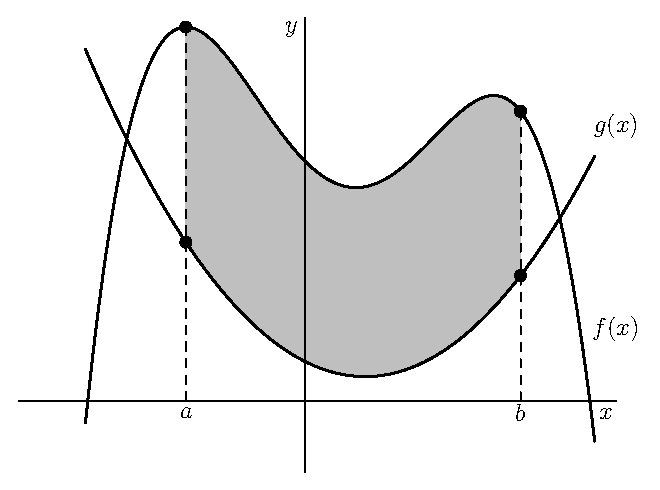
\includegraphics[width=400pt]{ChapterGeom/Figures/areabetweencurves.eps}
	\end{center}

\begin{example}{Quadrature of a Parabola}
 Suppose we wish to find the area \area{between curves} $f(x)=x$ and $g(x)=x^2$.  To accomplish this, we set the two formulas equal to each other to solve for the points of intersection.  The line and \conics{parabola} meet where  $$x^2=x \implies x^2-x=0 \implies x(x-1)=0 \implies x=0 \text{ or }  x=1.$$ 
Thus the points of intersection are at $(0,0)$ and $(1,1)$. 

	\begin{center}
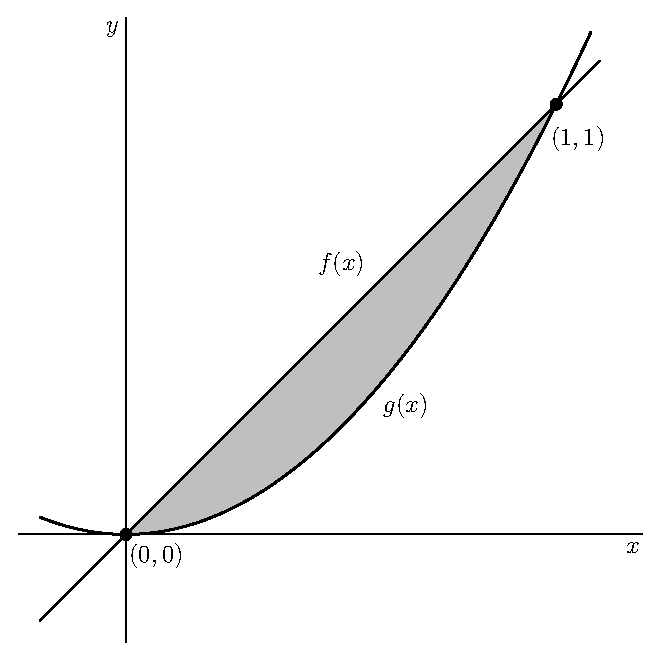
\includegraphics[width=300pt]{ChapterGeom/Figures/areabtparablin.eps}
	\end{center}
Thus, the area between curves is \begin{align*}
\int_{x=0}^{x=1}\left(x-x^2\right) \dif x &= \left. \frac{x^2}{2}-\frac{x^3}{3}\right]_{x=0}^{x=1} \\
&=\frac{1}{2}-\frac{1}{3}\\
&=\frac{1}{6}.
\end{align*}
\end{example}
\begin{comment}
\begin{exercise}{Area Between $x$ and $x^n$ \Coffeecup \Coffeecup}

For each of the listed $n\in \mathbb{N}$, take the following steps:

\begin{itemize}
\item Graph $f(x)=x$ and $g(x)=x^n$ on the same axes and shade the region bounded by the curves in the first quadrant.  Include labels of the intersection points of the curves.
\item Use an integral to find the area between curves.
\item Write the area as a decimal approximation.
\end{itemize}

Compile your results in the table below.

\begin{center}
\begin{tabular}{|c|c|c|c|} \hline
$n$ & Graph of $x$ and $x^n$ in QI & Area Between Curves in QI & Decimal Approximation \\ \hline 
& & & \\
& & & \\
3 & & & \\
& & & \\
& & & \\ \hline
& & & \\
& & & \\
4 & & & \\
& & & \\
& & & \\ \hline
& & & \\
& & & \\
5 & & & \\
& & & \\
& & & \\ \hline
& & & \\
& & & \\
6 & & & \\
& & & \\
& & & \\ \hline
& & & \\
& & & \\
7 & & & \\
& & & \\
& & & \\ \hline
& & & \\
& & & \\
8 & & & \\
& & & \\
& & & \\ \hline
& & & \\
& & & \\
9 & & & \\
& & & \\
& & & \\ \hline
& & & \\
& & & \\
10 & & & \\
& & & \\
& & & \\ \hline
\end{tabular}
\end{center}

\begin{itemize}
\item What does the area seem to be approaching as $n$ keeps getting larger?

\vspace{1in}

\item What shape does the region between the curves seem to be approaching as $n$ keeps getting larger?  Using just basic geometry, what would the area of that shape be?

\vspace{1in}

\end{itemize}

\end{exercise}

\end{comment}

Note that if the curves intersect multiple times, you might have to split the integral onto the corresponding intervals.  

\begin{example}{A Region with More Crossings}
 Find the area between the graphs of sine and cosine between $x=0$ and $x=2\pi$.

Again, to accomplish this, we set the two formulas equal to each other to solve for the points of intersection.  $$\sin(x)=\cos(x) \implies \tan(x)=1 \implies x=\pi/4  \text{ or }  x=5\pi/4$$ 
Thus the points of intersection are at $\left(\pi/4,\sqrt{2}/2\right)$ and $\left(5\pi/4,-\sqrt{2}/2\right)$. 

	\begin{center}
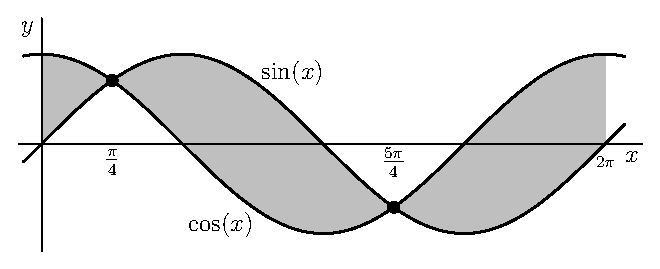
\includegraphics[width=300pt]{ChapterGeom/Figures/areabtsincos.eps}
	\end{center}

We now compute the area as follows: \begin{align*}
A&=\int_0^{\pi/4} \left(\cos(x)-\sin(x)\right) \dif x+\int_{\pi/4}^{5\pi/4} \left(\sin(x)-\cos(x)\right) \dif x+\int_{5\pi/4}^{2\pi} \left(\cos(x)-\sin(x)\right) \dif x \\
&=\left(\sin(x)+\cos(x)\right)|_0^{\pi/4} +\left(-\cos(x)-\sin(x)\right)|_{\pi/4}^{5\pi/4} +\left(\sin(x)+\cos(x)\right)|_{5\pi/4}^{2\pi}. 
\end{align*}

\end{example}
\begin{exercise}{Complete the Example \Coffeecup \Coffeecup }
Finish the computation and verify the area is 4$\sqrt{2}$.
\solushun{\begin{align*}
&\left(\sin(x)+\cos(x)\right)|_0^{\pi/4} +\left(-\cos(x)-\sin(x)\right)|_{\pi/4}^{5\pi/4} +\left(\sin(x)+\cos(x)\right)|_{5\pi/4}^{2\pi}\\
&=\left(\sin(\pi/4)+\cos(\pi/4)\right)-\left(\sin(0)+\cos(0)\right)\\
&\ \ +\left(-\cos(5\pi/4)-\sin(5\pi/4)\right)-\left(-\cos(\pi/4)-\sin(\pi/4)\right)\\
&\ \ +\left(\sin(2\pi)+\cos(2\pi)\right)-\left(\sin(5\pi/4)+\cos(5\pi/4)\right)\\
&=\left(\frac{\sqrt{2}}{2}+\frac{\sqrt{2}}{2}\right)-\left(0-1\right)\\
&\ \ +\left(-\frac{\sqrt{2}}{2}+\frac{\sqrt{2}}{2}\right)-\left(-\frac{\sqrt{2}}{2}-\frac{\sqrt{2}}{2}\right)\\
&\ \ +\left(0-1\right)-\left(-\frac{\sqrt{2}}{2}-\frac{\sqrt{2}}{2}\right)\\
&=\left(\sqrt{2}\right)-\left(1\right)\\
&\ \ +\left(\sqrt{2}\right)-\left(-\sqrt{2}\right)\\
&\ \ +\left(1\right)-\left(-\sqrt{2}\right)\\
&=4\sqrt{2}
\end{align*}
}{3in}
\end{exercise}

\begin{exercise}{A Common Mistake \Coffeecup}
 Briefly write in words, why would simply evaluating $$\int_{x=0}^{x=2\pi} \cos(x)-\sin(x) \dif x  $$ in the example above not give the area of the shaded region?

\solushun{Because the curves alternate which one is greater, the sign of the integral changes with each intersection. Thus, when $\sin(x)>\cos(x)$, the integral would be negative. So, simply summing would result in some canceling out, which would not give an accurate measure of the area between the two curves.\\}{1in}
\end{exercise}

\subsection{Area of a Circle}

Let's now prove an old friend, the formula for the \circles{area} \area{of a circle}!
\begin{exercise}{Area of a Circle \Coffeecup \Coffeecup }
\begin{itemize}
\item Recall the equation for a \conics{circle} of radius $r$ is $x^2+y^2=r^2$. Draw a diagram that shows that this equation is a consequence of the Pythagorean Theorem.  

\solushun{\\
\begin{center}
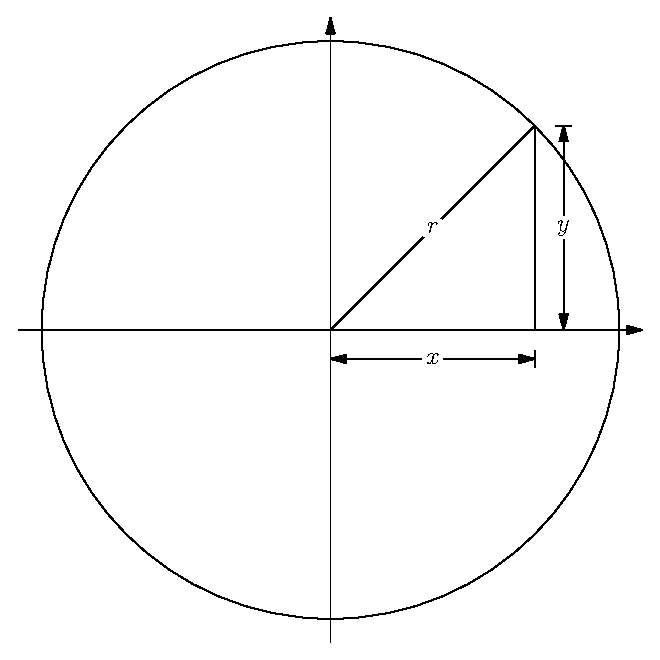
\includegraphics[width=200pt]{ChapterGeom/Figures/pythagcirc.eps}
\end{center}}{1in}

\item Solve for $y$ and note that the square root requires a ``plus or minus''.  To get the top curve $f(x)$, choose the positive square root.  To get the bottom curve $g(x)$, choose the negative square root.  Write your formulas for $f(x)$ and $g(x)$ below. \vspace*{.1in}
\begin{itemize}
\item Top Half: $f(x) = $
\vspace*{.1in}
\item Bottom Half: $g(x) = $
\vspace*{.1in}
\end{itemize}
\solushun{\vspace*{.1in}
\begin{itemize}
\item Top Half: $f(x) = \sqrt{r^2-x^2}$
\vspace*{.1in}
\item Bottom Half: $g(x) = -\sqrt{r^2-x^2}$
\vspace*{.1in}
\end{itemize}}{1in}

\item Use an integral to find the area between $f$ and $g$ to obtain the formula for the area of a circle of radius $r$.  

\solushun{\begin{align*}
\int_{-r}^{r}\sqrt{r^2-x^2}-\left(-\sqrt{r^2-x^2}\right)\dif x&=\int_{-r}^{r}2\sqrt{r^2-x^2}\dif\\
&=2\int_{-\pi/2}^{\pi/2}\sqrt{r^2-r^2\sin^2(\theta)}\cdot r\cos(\theta)\dif \theta\\
&=2\int_{-\pi/2}^{\pi/2}r^2\cos^2(\theta)\dif \theta\\
&=2r^2\int_{-\pi/2}^{\pi/2}\frac{1}{2}\left(1+\cos(2\theta)\right)\dif \theta\\
&=r^2\left[\theta+\frac{1}{2}\sin(2\theta)\right]_{-\pi/2}^{\pi/2}\\
&=r^2\left[\left(\frac{\pi}{2}+\frac{1}{2}\sin(\pi)\right)-\left(-\frac{\pi}{2}+\frac{1}{2}\sin(-\pi)\right)\right]\\
&=r^2\left[\left(\frac{\pi}{2}\right)-\left(-\frac{\pi}{2}\right)\right]\\
&=\pi r^2
\end{align*}}{2in}

\end{itemize}
\end{exercise}

\subsection{Some Other Regions for Practice}
Find the area between the following curves.  Graph the curves and shade the region! 
\begin{exercise}{Other Regions \Coffeecup \Coffeecup}

\begin{itemize}
\begin{comment}
\item $y=|x|$ and $y=\frac{1}{2}
x+1$
\vspace*{2in}

\item $y=\sqrt{x}$ and $y=\frac{1}{2}x^2$
\vspace*{2in}

\end{comment}
\item $ f(x)=x^3-x^2-x+1$ and $g(x)=x^3+x^2-x-1$
\solushun{
We start by identifying where the two graphs intersect, which we can accomplish by settings them equal and solving for $x$:
\begin{align*}
f(x)=&g(x)\\
x^3-x^2-x+1=&x^3+x^2-x-1\\
2=&2x^2\\
1=&x^2
x=\{-1,1\}
\end{align*}
So the bounds of integration are $-1,1$.
\begin{align*}
\int_{-1}^1 f(x)-g(x)\dif x&=\int_{-1}^1 x^3-x^2-x+1-(x^3+x^2-x-1)\dif x\\
&=\int_{-1}^1-2x^2+2\dif x\\
&=-2\int_{-1}^1x^2-1\dif x\\
&=-2\left[\frac{x^3}{3}-x\right]^1_{-1}\\
&=-2\left[\frac{1^3}{3}-1-\left(\frac{(-1)^3}{3}-(-1)\right)\right]\\
&=-2\left[-\frac{2}{3}-\frac{2}{3}\right]\\
&=\frac{8}{3}
\end{align*}
\begin{center}
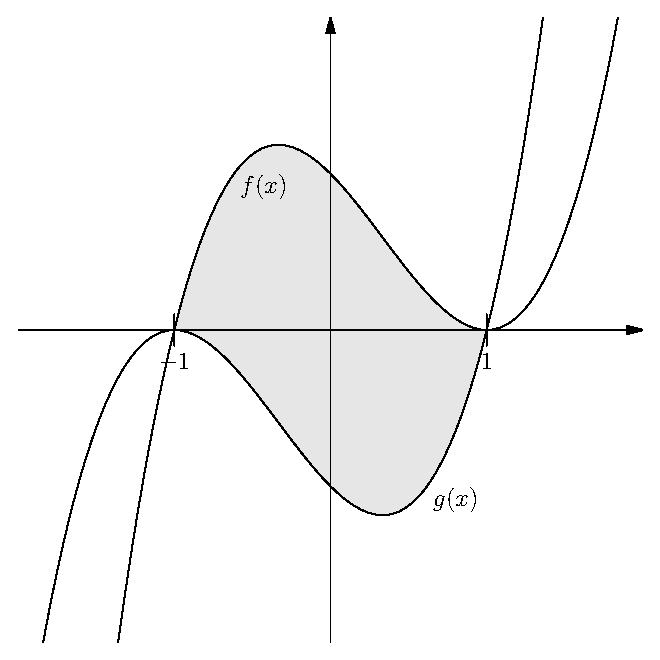
\includegraphics[width=300pt]{ChapterGeom/Figures/polyarea.eps}
\end{center}}{2in}

\item $y=\sqrt{1-x^2}$ and $y=1/2 $

\solushun{
Start by finding the bounds of integration by setting the two equations equal and finding $x$:
\begin{align*}
\sqrt{1-x^2}&=1/2\\
1-x^2&=\frac{1}{4}\\
\frac{3}{4}&=x^2\\
\pm\frac{\sqrt{3}}{2}=x
\end{align*}
Then, set up your integral, using the fact that we already found the antiderivative of a circle:
\begin{align*}
\int^{\frac{\sqrt{3}}{2}}_{-\frac{\sqrt{3}}{2}}\sqrt{1-x^2}-\frac{1}{2}\dif x&=\frac{1}{2}\left[\theta+\frac{1}{2}\sin(2\theta)\right]^{\pi/3}_{-\pi/3}-\frac{1}{2}\left[x\right]^{\sqrt{3}/2}_{-\sqrt{3}/2}\\
&=\frac{1}{2}\left[\frac{\pi}{3}+\frac{1}{2}\sin(\frac{2\pi}{3})-\left(-\frac{\pi}{3}+\frac{1}{2}\sin(-\frac{2\pi}{3})\right)\right]-\frac{1}{2}\left[\frac{\sqrt{3}}{2}-\left(-\frac{\sqrt{3}}{2}\right)\right]\\
&=\frac{1}{2}\left[\frac{\pi}{3}+\frac{1}{2}\frac{\sqrt{3}}{2}-\left(-\frac{\pi}{3}-\frac{1}{2}\frac{\sqrt{3}}{2})\right)\right]-\frac{\sqrt{3}}{2}\\
&=\frac{1}{2}\left[\frac{2\pi}{3}+\frac{\sqrt{3}}{2}\right]-\frac{\sqrt{3}}{2}\\
&=\frac{\pi}{3}-\frac{\sqrt{3}}{4}
\end{align*}
\begin{center}
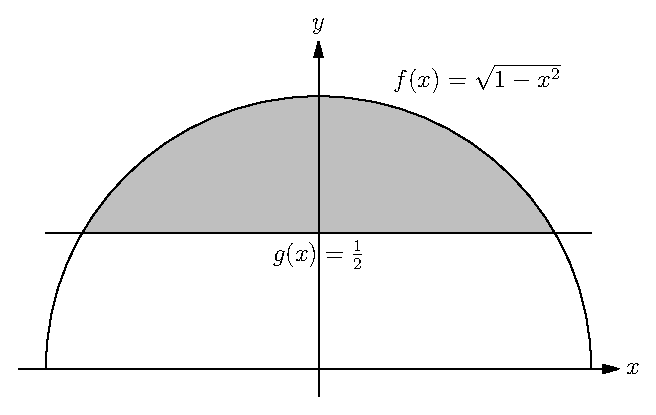
\includegraphics[width=300pt]{ChapterGeom/Figures/clippedcirc_cropped.eps}
\end{center}
}{2in}
\item $y=\tan(x)$ restricted to the domain $\left(-\pi/2,\pi/2\right)$ and $y=\frac{4}{\pi}x$

\solushun{First, find the point of intersection. A good way to do this is to graph both functions, and notice that they seem to intersect when they both equal $1$. Then, test this out by setting them both equal to 1 and solving for $x$:
$$\tan(x)=1\implies\arctan(1)=x\\
x=\frac{\pi}{4}
$$
$$\frac{4}{\pi}x=1\implies x=\frac{\pi}{4}$$
So, the functions intersect at $(\frac{\pi}{4},1)$.
A similar process produces another intersection at $(-\frac{\pi}{4},-1)$.

We need to split the integral because the functions cross at $x=0$:
$$\int_{-\pi/4}^0\tan(x)-\frac{4}{\pi}x\dif  x+\int_0^{\pi/4}\frac{4}{\pi}x-\tan(x) \dif x
$$

This gets a little messy, but since the graph is symmetrical, we can save ourselves some trouble by simply evaluating the easier integral and then doubling it.

\begin{align*}
\int_{-\pi/4}^0\tan(x)-\frac{4}{\pi}x\dif x&=\left[-\ln|\cos(x)|-\frac{2}{\pi}x^2\right]_{-\pi/4}^0\\
&=-\ln|\cos(0)|-\frac{2}{\pi}\cdot0^2-\left(-\ln\left|\cos\left(-\frac{\pi}{4}\right)\right|-\frac{2}{\pi}\left(-\frac{\pi}{4}\right)^2\right)\\
&=\ln\left|\cos\left(-\frac{\pi}{4}\right)\right|+\frac{2}{\pi}\left(-\frac{\pi}{4}\right)^2\\
&=\ln\left|\frac{\sqrt{2}}{2}\right|+\frac{2}{\pi}\left(\frac{\pi^2}{16}\right)\\
&=\ln\left|\frac{\sqrt{2}}{2}\right|+\frac{\pi}{8}
\end{align*}
So the final integral is:
$$2\left(\ln\left|\frac{\sqrt{2}}{2}\right|+\frac{\pi}{8}\right)=\left(\ln\left|\frac{1}{2}\right|+\frac{\pi}{4}\right)$$
We can simplify the logarithm a bit:
$$\left(\ln\left|\frac{1}{2}\right|+\frac{\pi}{4}\right)=\ln|1|-\ln|2|+\frac{\pi}{4}=\frac{\pi}{4}-\ln|2|$$
\begin{center}
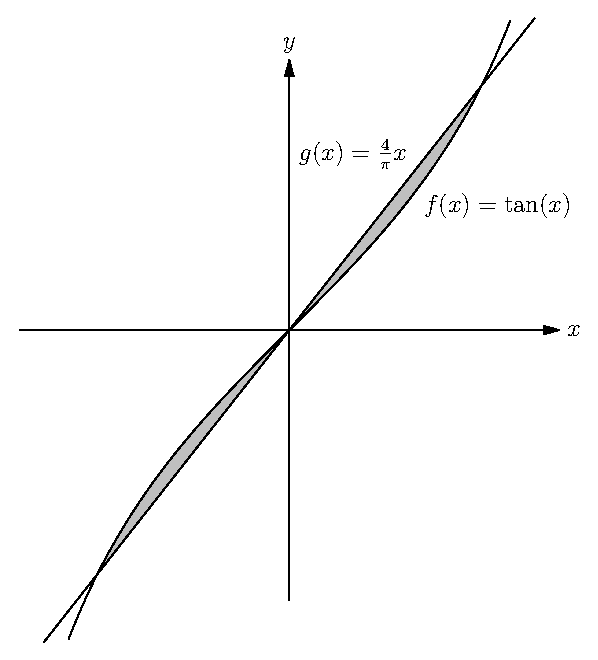
\includegraphics[width=300pt]{ChapterGeom/Figures/tangentarea.eps}
\end{center}
}{2in}

\end{itemize}
\AnswerKeyEntry{\textbullet The curves $y=x^3+x^2-x-1$ and $y=x^3-x^2-x+1$ intersect on the $x$ axis at -1 and 1 and have area 8/3 between them. 
\textbullet The area inside the unit circle but above the line $y=1/2$ is $\pi/3-\sqrt{3}/4$.
\textbullet Notice graphically that the curves intersect at $x=\pm \pi/4$.  The area between curves is $\pi/4-\ln(2)$.}
\end{exercise}

%KHALED:^^^^ Need figures for last 2 problems
%\section{Arc Length, Surface Area, Volume}
In this section, we will look at four formulas built out of integrals.  Let's just get them all down here, and we'll play with them and explain them as we go!
\begin{enumerate}
\item {\bf Arc Length:} The \arclength{length of the graph of a function} $f(x)$ from the point $\left(a,f(a)\right)$ to the point $\left(b,f(b)\right)$ is given by $ L= \int_{x=a}^{x=b} \sqrt{1+\left( f'(x)\right)^2 } \dif x $.
	\begin{center}
        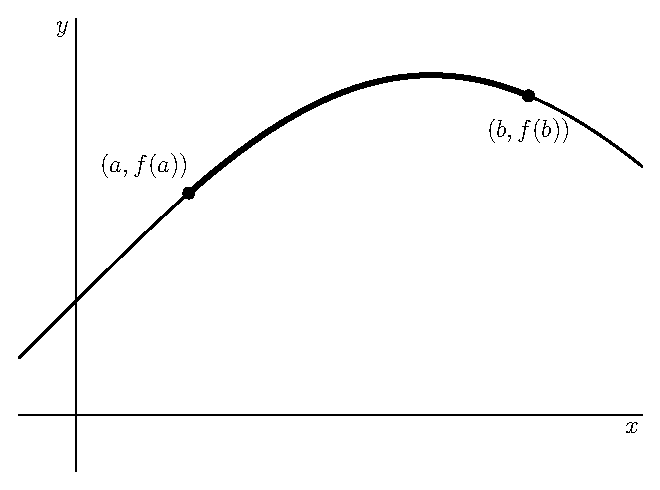
\includegraphics[width=300pt]{ChapterGeom/Figures/arclength.eps}
	\end{center}
\item {\bf Surface Area of a Surface of Revolution:} If the graph of $f(x)$ from the point $\left(a,f(a)\right)$ to the point $\left(b,f(b)\right)$ is revolved around the $y$-axis, the \area{surface area} is given by $$ SA= \int_{x=a}^{x=b} 2 \pi x\sqrt{1+\left( f'(x)\right)^2 } \dif x .$$ 
% \todo[inline]{What if it is revolved around the x axis or around another line? Or will that be covered later?}
%TODO list! :) Yes one of my todo list agenda items is to add that kind of computation in, and show how any such computation is always just a u-sub away from using the y-axis.  That a change of coordinates can always make the y-axis be your rotation axis.
	\begin{center}
        \includegraphics[width=300pt]{ChapterGeom/Figures/surfaceareaASY.eps}
	\end{center}
    
\item {\bf Volume:} We have two distinct methods for volume.

\begin{itemize}

\item {\bf Cross Sections:}  Suppose a 3D solid starts at $x=a$ and ends at $x=b$ and the function $A(x)$ represents the area of the cross-section at location $x$, then the solid has volume $V=\int_{x=a}^{x=b}A(x) \dif x $. 

	\begin{center}
		\includegraphics[width=300pt]{ChapterGeom/Figures/CrossSections.eps}
	\end{center}
\item {\bf Cylindrical Shells:}  If the region under of $f(x)$ from the point $\left(a,f(a)\right)$ to the point $\left(b,f(b)\right)$ is revolved around the $y$-axis, the volume is given by $ V= \int_{x=a}^{x=b} 2 \pi x f(x) \dif x $.
    
    \begin{center}
		\includegraphics[width=300pt]{ChapterGeom/Figures/CylindShells1.eps}
	\end{center}

\end{itemize}
\end{enumerate}

Let's now do a little example of each and throughout analyzing the example, convince ourselves that each formula is correct.

\subsection{The Arc Length Formula}\label{ArcLength}

The \integ{arc length} formula is in essence the following idea: to approximate the length of a curve, let's split it up into line segments, compute each of the line segment lengths using the Pythagorean Theorem, and then take the limit as the number of line segments goes to infinity.  Time to carry this out on a good old vanilla \conics{parabola}!
\begin{exercise}{Approximating the \arclength{Length of a Parabola} with Line Segments \Coffeecup \Coffeecup }

\begin{itemize}
\item On the axes below, graph the function $f(x)=x^2$ from the point $A=(0,0)$ to $E=(1,1)$.  Estimate the length of this arc by just connecting those two endpoints with a straight line and calculating its length via the Pythagorean Theorem.

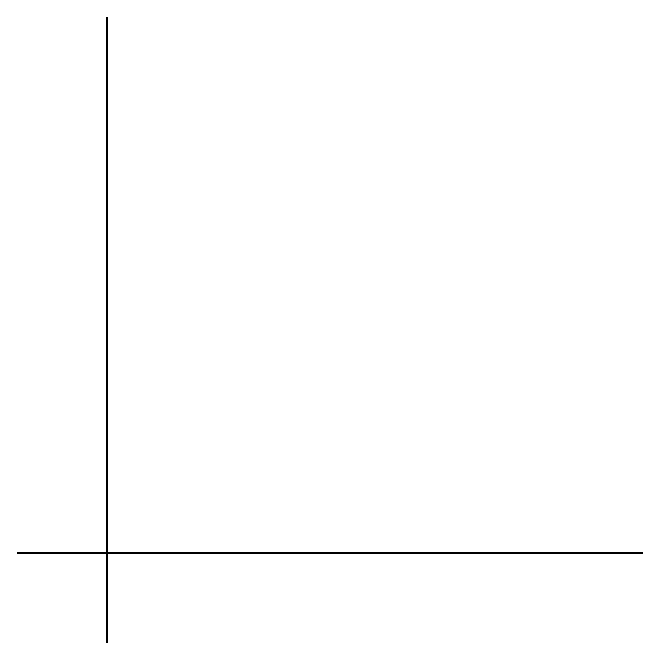
\includegraphics[scale=0.5]{quad1.eps}
\solushun{
\begin{center}
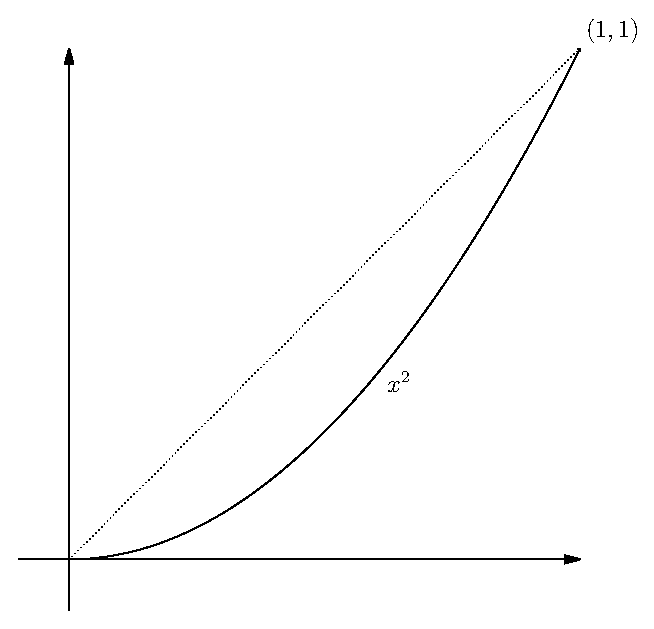
\includegraphics[scale=0.5]{ChapterGeom/Figures/squaredlength.eps}
\end{center}
The length is $\sqrt{1^2+1^2}=\sqrt{2}$.\\
}{0in}

\item Again graph the function $f(x)$ from the point $A=(0,0)$ to $E=(1,1)$, but on this graph also include a label for the point $C=(\frac{1}{2},\frac{1}{4})$.  This time lets estimate the length of this arc using two line segments.  Specifically, calculate the lengths of $\overline{AC}$ and $\overline{CE}$ and add their lengths to estimate the \parabola{arc length} of the parabola.  Did your estimate go up or down by using two segments instead of just one?  Does this make sense?

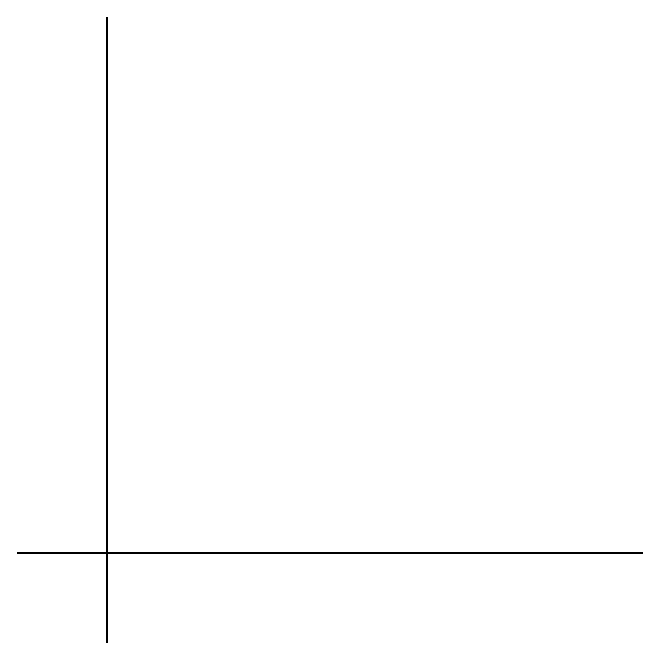
\includegraphics[scale=0.5]{quad1.eps}
\solushun{\begin{center}
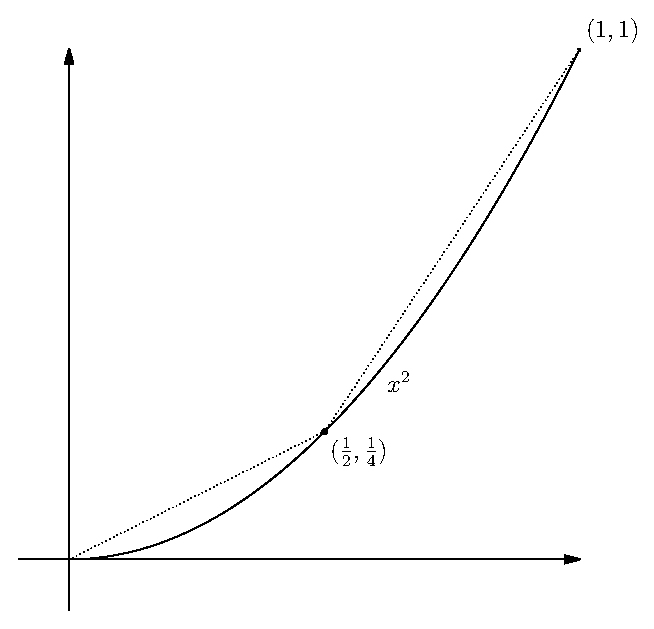
\includegraphics[scale=0.5]{ChapterGeom/Figures/squaredlength_2.eps}
\end{center}
The length is
$$
\sqrt{\left(\frac{1}{2}\right)^2+\left(\frac{1}{4}\right)^2}+\sqrt{\left(\frac{1}{2}\right)^2+\left(\frac{3}{4}\right)^2}
= \sqrt{\frac{1}{4}+\frac{1}{16}}+\sqrt{\frac{1}{4}+\frac{9}{16}}
= \sqrt{\frac{5}{16}}+\sqrt{\frac{13}{16}}
= \frac{\sqrt{5}+\sqrt{13}}{4}
$$
This is approximately $\frac{5.84}{4}\approx1.46$, which is slightly longer than $\sqrt{2}\approx1.41$. This makes sense, since the extra leg means the two paths cover more distance than the single path.\\
}{0in}

\item Define $A$, $C$, and $E$ as before.  Define $B$ to be the point on the parabola with $x$-coordinate one-fourth and $D$ to be the point on the parabola with $x$-coordinate three-fourths.  Again estimate the length of the curve by adding the lengths of the segments  $\overline{AB}$, $\overline{BC}$, $\overline{CD}$, and  $\overline{DE}$.  What happens to the estimate?  Did it increase or decrease?  Did it get more or less accurate as compared to the true arc length?

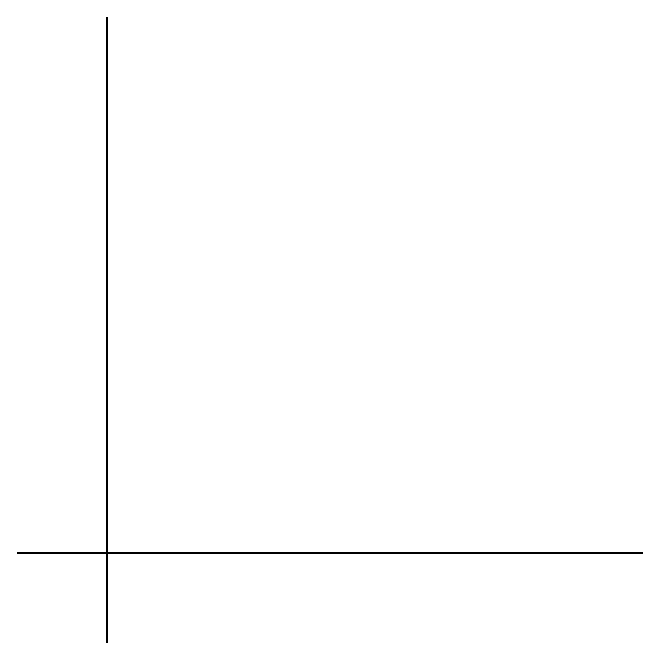
\includegraphics[scale=0.5]{quad1.eps}
\solushun{\begin{center}
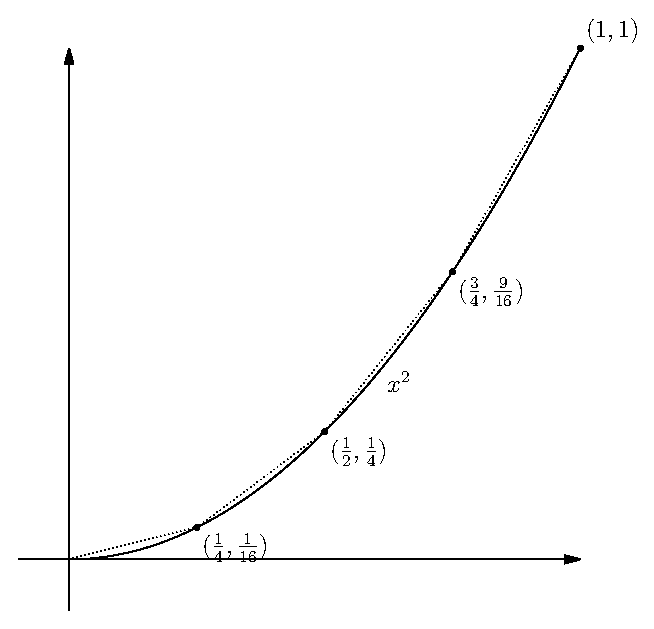
\includegraphics[scale=0.5]{ChapterGeom/Figures/squaredlength_3.eps}
\end{center}
The length is:
$$\sqrt{\left(\frac{1}{4}\right)^2+\left(\frac{1}{16}\right)^2}+\sqrt{\left(\frac{1}{4}\right)^2+\left(\frac{3}{16}\right)^2}+\sqrt{\left(\frac{1}{4}\right)^2+\left(\frac{5}{16}\right)^2}+\sqrt{\left(\frac{1}{4}\right)^2+\left(\frac{7}{16}\right)^2}$$
$$=\frac{1}{16}\left(\sqrt{17}+5+\sqrt{41}+\sqrt{65}\right)\approx1.47$$
}{0in}
\end{itemize}
\end{exercise}

Ok, at this point we get the idea.  More line segments will result in a more accurate approximation, and the limit of these approximations as the number of line segments goes to infinity will produce the exact result.  Here is a \arclength{derivation} that shows this process will result in exactly the right formula.

Let $x_0,x_1,x_2,\ldots,x_n$ be equally spaced points along the $x$-axis from $a$ to $b$.  That is, $x_0=a$, $x_n=b$, and for each $i\in\lbrace 0,1,2,\ldots , n-1 \rbrace$, $\Delta x = x_{i+1}-x_{i}=\frac{b-a}{n}$.

With this setup, if we want the length of a line segment connecting points $x_{i+1}$ and $x_{i}$, we would use the Pythagorean Theorem to obtain: 
$$\sqrt{\left(\Delta x\right)^2+\left(f\left(x_{i+1}\right)-f\left(x_i\right)\right)^2 } $$ as the length.


\begin{align*}
L&=\lim_{n\rightarrow \infty}\sum_{i=0}^{n-1} \sqrt{\left(\Delta x\right)^2+\left(f\left(x_{i+1}\right)-f\left(x_i\right)\right)^2 } \\
&=\lim_{n\rightarrow \infty}\sum_{i=0}^{n-1} \sqrt{1+\frac{\left(f\left(x_{i+1}\right)-f\left(x_i\right)\right)^2}{\left( \Delta x\right)^2} } \sqrt{\left(\Delta x\right)^2} \\
&=\lim_{n\rightarrow \infty}\sum_{i=0}^{n-1} \sqrt{1+\left( \frac{f\left(x_{i+1}\right)-f\left(x_i\right)}{\Delta x}\right)^2 } \Delta x \\
&=\int_{x=a}^{x=b} \sqrt{1+\left( f'(x)\right)^2 } \dif x
\end{align*}

And thus we have our formula for arc length!

\FormulaBox{Arc Length Formula}{
The graph of the function $f(x)$ from $x=a$ to $x=b$ has length $L= \int_{x=a}^{x=b} \sqrt{1+\left( f'(x)\right)^2 } \dif x$.
}

\begin{exercise}{Exact Arc Length of the Parabola \Coffeecup \Coffeecup \Coffeecup}

\begin{itemize}
\item  We now apply this integral formula to calculate the exact length of our parabolic segment.  Plugging in the formula $f(x)=x^2$ into the arc length integral, we obtain:

$$ L= \int_{x=0}^{x=1} \sqrt{1+\left( 2x\right)^2 } \dif x$$

Finish the evaluation of this integral.  ({\bf Hint:}  The \secant{arc length integral} will be quite difficult!  See Example \ref{reappear}.\ref{seccubed} for help.)  

\solushun{\begin{align*}
L&= \int_{x=0}^{x=1} \sqrt{1+\left( 2x\right)^2 } \dif x\\
&=\int_{x=0}^{x=1} \sqrt{1+4x^2 } \dif x\\
&=\int_{x=0}^{x=1} \sqrt{1+4\left(\frac{1}{2}\tan(\theta)\right)^2 }\cdot \frac{1}{2}\sec^2(\theta) \dif x\tag{Let $x=\frac{1}{2}\tan(\theta)$}\\
&=\frac{1}{2}\int_{x=0}^{x=1} \sqrt{\sec^2(\theta)}\cdot \sec^2(\theta) \dif x\\
&=\frac{1}{2}\int_{x=0}^{x=1} \sec^3(\theta) \dif x\\
&=\frac{1}{2}\left[\frac{1}{2}\left(\sec(\theta)\tan(\theta)+\ln|\sec(\theta)+\tan(\theta)|\right)\right]_{x=0}^{x=1}\tag{From \ref{reappear}\ref{seccubed}}\\
&=\frac{1}{4}\left[\left(\sqrt{4x^2+1}2x+\ln|\sqrt{4x^2+1}+2x|\right)\right]_{x=0}^{x=1}\tag{$\tan\theta=2x\implies\tan^2\theta=4x^2\implies\sec^2\theta=4x^2+1$}\\
&=\frac{2\sqrt{5}+\ln|\sqrt{5}+2|}{4}-\left(\frac{2(0)\sqrt{1}+\ln|\sqrt{1}+0|}{4}\right)\\
&=\frac{2\sqrt{5}+\ln|\sqrt{5}+2|}{4}\\
&\approx1.48
\end{align*}}{3in}

\item How does the exact value of the arc length compare to the approximations?
\solushun{The exact value is very close to the approximations, but it is slightly larger than the approximations we used.\\}{0.25in}
\end{itemize}
\AnswerKeyEntry{The exact arc length is $\frac{2\sqrt{5}+\ln\left| 2+\sqrt{5}\right|}{4}$.}
\end{exercise}

\begin{example}{Arc Length of a Hyperbola}\label{HyperBocaBola}

	\begin{wrapfigure}{r}{0.2\textwidth}
    	\centering
		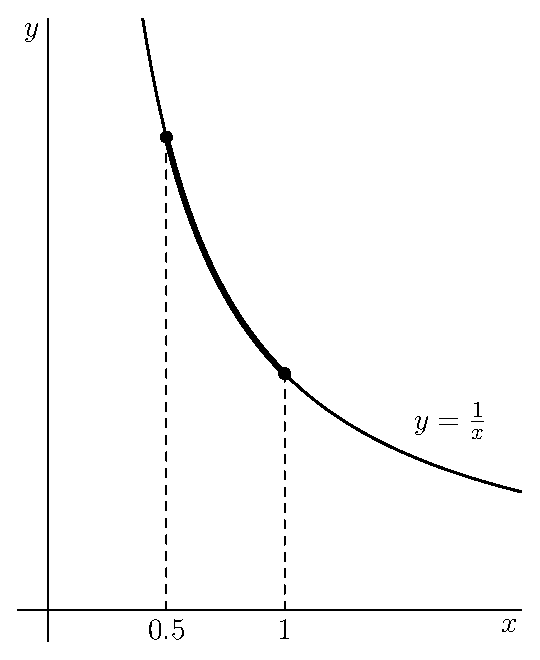
\includegraphics[width=0.2\textwidth]{ChapterGeom/Figures/HyperbolaArcLength}
	\end{wrapfigure}

Suppose we wish to find the arc length $L$ of the hyperbola $$xy=1$$ between the points $\left(\frac{1}{2},2\right)$ and $\left(1,1\right)$.  We begin by solving for the $y$ coordinate in order to express this section of the graph as a function.  Dividing both sides by $x$ produces $$y=f(x)=\frac{1}{x}. $$  We wish to find the length of the graph of this function between $x=\frac{1}{2}$ and $x=1$.  We plug into the arc length formula to obtain $$L= \int_{x=1/2}^{x=1} \sqrt{1+\left( f'(x)\right)^2 } \dif x= \int_{x=1/2}^{x=1} \sqrt{1+\left( -\frac{1}{x^2}\right)^2 } \dif x=\int_{x=1/2}^{x=1} \frac{\sqrt{1+x^4}}{x^2} \dif x. $$ Though we have demonstrated how to set up the arc length integral, it turns out that this integral is quite difficult to evaluate!  In particular, the integrand has no closed form antiderivative.  We will revisit this example in Section \ref{PowerSeriesSubstitution} where we'll have extra tools. 
\end{example}
\begin{exercise}{Checking the Example \Coffeecup}
In the above example...
\begin{itemize}
\item Verify the algebra on the last step, where the integrand is simplified from $\sqrt{1+\left( -\frac{1}{x^2}\right)^2 }$ to $\frac{\sqrt{1+x^4}}{x^2}$. 

\solushun{\begin{align*}
\sqrt{1+\left( -\frac{1}{x^2}\right)^2 }&=\sqrt{1+\frac{1}{x^4} }\\
&=\sqrt{\frac{x^4+1}{x^4} }\\
&=\frac{\sqrt{1+x^4}}{x^2}
\end{align*}}{.5in}

\item Try evaluating the integral via the trigonometric substitution $x=\sqrt{\tan\left(\theta\right)}$.  It may look promising at first!  However, where do you get stuck?

\solushun{\begin{align*}
\int_{x=1/2}^{x=1}\frac{\sqrt{1+x^4}}{x^2}\dif x&=\int\frac{\sqrt{1+\left(\sqrt{\tan\theta}\right)^4}}{\left(\sqrt{\tan\theta}\right)^2}\cdot\frac{\sec^2\theta}{2\sqrt{\tan\theta}}\dif \theta\tag{$x=\sqrt{\tan\theta}$}\\
&=\int_{x=1/2}^{x=1}\frac{\sqrt{1+\tan^2\theta}}{\tan\theta}\cdot\frac{\sec^2\theta}{2\sqrt{\tan\theta}}\dif \theta\\
&=\int_{x=1/2}^{x=1}\frac{\sec^3\theta}{2\left(\tan\theta\right)^{\frac{3}{2}}}\dif \theta\\
&=\frac{1}{2}\int_{x=1/2}^{x=1}\frac{1}{\cos^3\theta\frac{\left(\sin\theta\right)^\frac{3}{2}}{\left(\cos\theta\right)^\frac{3}{2}}}\dif \theta\\
&=\frac{1}{2}\int_{x=1/2}^{x=1}\frac{1}{\left(\cos\theta\sin\theta\right)^\frac{3}{2}}\dif \theta\\
\end{align*}
We get stuck because we don't have a way to evaluate integrals of fractional powers of trig functions.\\}{1in}

\end{itemize}
\end{exercise}
\subsection{Circumference of a Circle }
We now use the arc length integral to compute the \circles{circumference} of a circle.  Though one can take the formula for the circumference of a circle simply as the definition of $\pi$, it is still nice to go through this as proof of concept.  

\begin{exercise}{Circumference of a Circle \Coffeecup \Coffeecup}
\begin{itemize}
\item Use the arc length formula to calculate the circumference of a circle with radius $r$.

\solushun{
Our equation of a circle in terms of $x$ and $r$ can be derived from the standard equation of a circle:
$$x^2+y^2=r^2\implies y=\sqrt{r^2-x^2}$$
Taking the derivative gives $$f'(x)=\frac{-2x}{2\sqrt{r^2-x^2}}=\frac{-x}{\sqrt{r^2-x^2}}$$
To simplify the calculation a bit, we will only find the arc length for the top right quarter of the circle, then multiply the result by $4$.
\begin{align*}
4\int^{x=r}_{x=0}\sqrt{1+\left(f'(x)\right)^2}\dif x&=4\int^{x=r}_{x=0}\sqrt{1+\left(\frac{-x}{\sqrt{r^2-x^2}}\right)^2}\dif x\\
&=4\int^{x=r}_{x=0}\sqrt{1+\frac{x^2}{r^2-x^2}}\dif x\\
&=4\int^{x=r}_{x=0}\sqrt{\frac{r^2-x^2+x^2}{r^2-x^2}}\dif x\\
&=4\int^{x=r}_{x=0}\sqrt{\frac{r^2}{r^2-x^2}}\dif x\\
&=4r\int^{x=r}_{x=0}\sqrt{\frac{1}{r^2-x^2}}\dif x\\
&=4r\int^{\theta=\pi/2}_{\theta=0}\sqrt{\frac{1}{r^2-\left(r\sin(\theta)\right)^2}}\cdot r\cos(\theta)\dif \theta\tag{Let $x=r\sin(\theta)$}\\
&=4r\int^{\theta=\pi/2}_{\theta=0}\frac{r\cos(\theta)}{r\cos(\theta)} \dif \theta\tag{Let $x=r\sin(\theta)$}\\
&=4r\left[\theta\right]^{\pi/2}_{0}\\
&=4r\left[\frac{\pi}{2}-0\right]\\
&=2\pi r\\
\end{align*}}{2in}

\item Take the derivative of your formula for area of a circle with respect to $r$.  How does it relate to your formula for the circumference of a circle?  Draw a picture and indicate why this freakish coincidence actually geometrically makes sense.

\solushun{$$\dfrac{\dif}{\dif r}\pi r^2=2\pi r$$
The derivative of the equation for area of a circle is the same  as the equation for the circumference of a circle. The definition of the derivative suggests that the derivative the area of a circle of radius $r$ is the limit of the difference between that circle and a slightly larger circle of radius $r+\Delta r$ as $\Delta r$ approaches 0. This can be visualized as cutting out the smaller circle from the larger one, and investigating what happens as the larger circle approaches the size of the smaller one.
\begin{center}
$$\dfrac{\dif}{\dif r}\pi r^2=\lim_{\Delta r\to0}\frac{\pi (r+\Delta r)^2-\pi r^2}{\Delta r}=\pi\lim_{\Delta r\to0}\frac{r^2+2r\Delta r+\Delta r^2- r^2}{\Delta r}=\pi\lim_{\Delta r\to0}2r+\Delta r=2\pi r$$
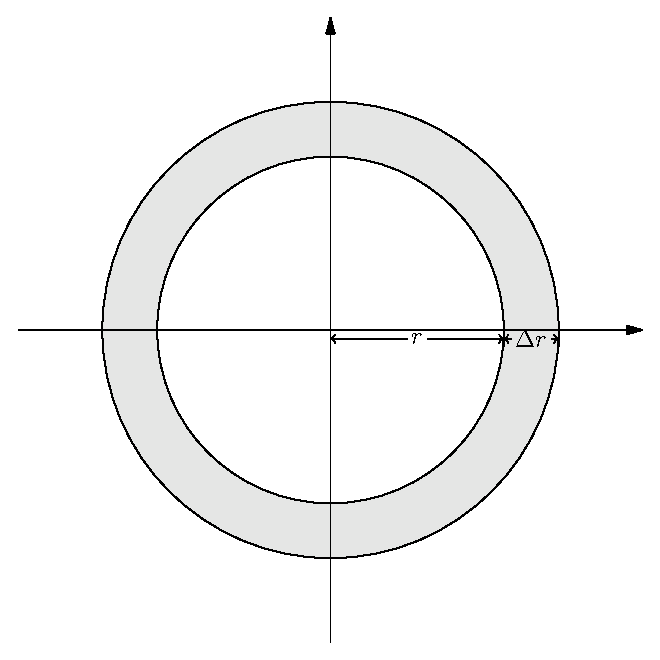
\includegraphics[scale=0.5]{ChapterGeom/Figures/circderiv.eps}
\end{center}}{1in}
\end{itemize}
\end{exercise}

\subsection{Lengths of Some Other Fun Arcs}
\begin{exercise}{Other Arcs \Coffeecup \Coffeecup \Coffeecup}

Draw the graph and compute the length of each of the following arcs using our arc length formula.
\begin{itemize}
\item Line segment from a point $(x_0,y_0)$ to a point $(x_1,y_1) $.  ({\bf Hint:} To get your function, use the point-slope form of a line and then solve for $y$.)  How does this compare to the length the Pythagorean Theorem would give you?

\solushun{
\begin{center}
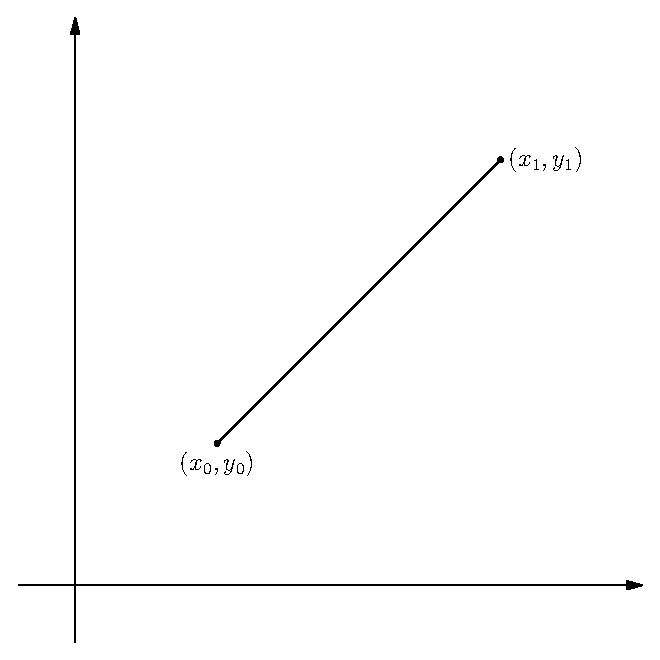
\includegraphics[scale=1]{ChapterGeom/Figures/linearc.eps}
\end{center}
$$(y-y_1)=m(x-x_1)\implies y=\frac{y_1-y_0}{x_1-x_0}x+y_1=f(x)$$
$$f'(x)=\frac{y_1-y_0}{x_1-x_0}$$
\begin{align*}
\int^{x_1}_{x_0}\sqrt{1+\left(\frac{y_1-y_0}{x_1-x_0}\right)^2}\dif x&=\sqrt{1+\left(\frac{y_1-y_0}{x_1-x_0}\right)^2}\left.x\right|^{x_1}_{x_0}\\
&=\sqrt{\frac{(x_1-x_0)^2+(y_1-y_0)^2}{(x_1-x_0)^2}}\left(x_1-x_0\right)\\
&=\frac{\sqrt{(x_1-x_0)^2+(y_1-y_0)^2}}{(x_1-x_0)^2}\left(x_1-x_0\right)\\
&=\sqrt{(x_1-x_0)^2+(y_1-y_0)^2}
\end{align*}
This is what we would get from the Pythagorean Theorem.\\}{2in}

\item The graph of $f(x)=\ln(x)$ from $x=1$ to $x=e$.  Take an approximation using two line segments, and then get the exact length using an arc length integral.  How do they compare?

\solushun{
\begin{center}
\includegraphics[scale=1]{ChapterGeom/Figures/lnarc.eps}
\end{center}
\begin{align*}
\int^e_1\sqrt{1+\left(\frac{1}{x}\right)^2}\dif x &= \int^e_1\sqrt{\frac{x^2+1}{x^2}}\dif x\\
\text{Let } x=\tan(\theta), \dif x=\sec^2(\theta)\dif\theta. \text{Then: }\\
\int^e_1\sqrt{\frac{x^2+1}{x^2}}\dif x&=\int^{x=e}_{x=1}\sqrt{\frac{\tan^2(\theta)+1}{\tan^2(\theta)}}\sec^2(\theta)\dif\theta\\
&=\int^{x=e}_{x=1}\frac{\sec^3(\theta)}{\tan(\theta)}\dif\theta\\
&=\int^{x=e}_{x=1}\sec^2(\theta)\csc(\theta)\dif\theta\\
\text{Now via IBP, let }\\
u=\csc(\theta), \dif u=-\csc(\theta)\cot(\theta), \\
v=\tan(\theta), \dif v =\sec^2(\theta)\\
\int^{x=e}_{x=1}\sec^2(\theta)\csc(\theta)\dif\theta&=\csc(\theta)\tan(\theta)+\int^{x=e}_{x=1}\tan(\theta)\csc(\theta)\cot(\theta)\dif\theta\\
&=\csc(\theta)\tan(\theta)+\int^{x=e}_{x=1}\csc(\theta)\dif\theta\\
&=\csc(\theta)\tan(\theta)-\ln\left|\csc(\theta)+\cot(\theta)\right|^{x=e}_{x=1}\\
\text{Draw a triangle to see that }\\
\csc(\theta)=\frac{\sqrt{x^2+1}}{x}\\
\tan(\theta)=x\\
\cot(\theta)=\frac{1}{x}\\
\text{Then: }\\
\csc(\theta)\tan(\theta)-\ln\left|\csc(\theta)+\cot(\theta)\right|^{x=e}_{x=1}&=\sqrt{x^2+1}-\ln\left|\frac{\sqrt{x^2+1}+1}{x}\right|^{x=e}_{x=1}\\
&=\left.\sqrt{x^2+1}-\ln\left|\sqrt{x^2+1}+1\right|-\ln|x|\right|^{x=e}_{x=1}\\
&=\sqrt{e^2+1}-\ln\left|\sqrt{e^2+1}+1\right|-\ln|e|-\left(\sqrt{1+1}-\ln\left|\sqrt{1+1}+1\right|-\ln|1|\right)\\
&=\sqrt{e^2+1}-\ln\left|\sqrt{e^2+1}+1\right|-1-\sqrt{2}+\ln\left|\sqrt{2}+1\right|\\
&\approx 2.003497
\end{align*}
To make the integral look like the nice symmetrical answer in the answer key requires some manipulation:
\begin{align*}
\sqrt{x^2+1}-\ln\left|\frac{\sqrt{x^2+1}+1}{x}\right|&=\sqrt{x^2+1}+\ln\left|\frac{x}{\sqrt{x^2+1}+1}\right|\\
&=\sqrt{x^2+1}+\frac{1}{2}\ln\left|\frac{x^2}{\left(\sqrt{x^2+1}+1\right)^2}\right|\\
&=\sqrt{x^2+1}+\ln\left|\frac{x^2+1-1}{\left(\sqrt{x^2+1}+1\right)^2}\right|\\
&=\sqrt{x^2+1}+\ln\left|\frac{\sqrt{x^2+1}^2-1^2}{\left(\sqrt{x^2+1}+1\right)^2}\right|\\
&=\sqrt{x^2+1}+\ln\left|\frac{\left(\sqrt{x^2+1}-1\right)\left(\sqrt{x^2+1}+1\right)}{\left(\sqrt{x^2+1}+1\right)^2}\right|\\
&=\sqrt{x^2+1}+\ln\left|\frac{\sqrt{x^2+1}-1}{\sqrt{x^2+1}+1}\right|
\end{align*}
}{3in}

\item The graph of $f(x)=e^x$ from $x=0$ to $x=1$.

\solushun{
Since the natural logarithm is the inverse of the natural exponential function, the length of the arc from corresponding segments will be the same. In this case, that's exactly what we have, since $\ln(1)=0, \ln(e)=1$.

So the arc length of $e^x$ from $x=0$ to $x=1$ is also approximately 2.003497.

To be precise, we could use the same formula we got above, and just set our bounds to be the value of the exponential at the endpoints of our range. That is, the arc length of $e^x$ from $x=a$ to $x=b$ with $b>a$ is:
$$\left[\sqrt{x^2+1}+\ln\left|\frac{\sqrt{x^2+1}-1}{\sqrt{x^2+1}+1}\right|\right]^{e^b}_{e^b}$$
Actually calculating the integral reveals an interesting connection between the two.
$$\int\sqrt{1+e^{2x}}\dif x = \sqrt{1+e^{2x}}+1+\ln\left|\frac{e^{2x}}{\sqrt{1+e^{2x}}+1}\right|+C$$
The actual process involves 3 rounds of $u$-substitutions. This is a good example of where clever use of previous results can save you a lot of time and effort.\\
}{1in}

%KHALED: I need to check and confirm that last integral of the arc length of e^x

\end{itemize}

\AnswerKeyEntry{The length of the graph of the natural logarithm from (1,0) to (e,1) is $$\sqrt{e^2+1}+\frac{1}{2}\ln\left| \frac{\sqrt{e^2+1}-1}{\sqrt{e^2+1}+1}\right|-\sqrt{2}+\frac{1}{2}\ln\left| \frac{\sqrt{2}+1}{\sqrt{2}-1}\right| $$ which is roughly 2.003497.  Also, notice that the natural exponential function is just the inverse of the natural logarithm; think about what this means regarding arc length!}
\end{exercise}

\subsection{Surface Area}

For the \integ{surface area} of a surface of revolution, we use the \surfacearea{frustum of a right circular cone} as the object that approximates the surface, much as we used line segments for arc length.  Thus, to get off the ground, we must figure out what the \cone{surface area of a frustum} is.  Suppose it has inner radius $r$ and outer radius $R$ and let $L$ be the diagonal length, top to bottom, of the frustum.  Project the shape onto a flat plane sitting under it to produce a washer whose outer radius is $R$ and inner radius is $r$.

	\begin{center}
		\includegraphics[width=300pt]{ChapterGeom/Figures/frustraproj.eps}
	\end{center} 

Notice that the washer in the plane has area $\pi (R^2-r^2)$.  Also, the radial lengths got uniformly scaled by a factor of $\frac{L}{R-r}$, since every segment of length $R-r$ got stretched into a segment of length $L$.  Thus we have that the area of the frustum is $\frac{L}{R-r}\cdot \pi (R^2-r^2)$, which simplifies to: $$SA=\pi L (R+r) $$

\begin{exercise}{\parabola{Surface Area of a Paraboloid} \Coffeecup \Coffeecup \Coffeecup}
To test this out, consider the parabola $y=x^2$ from $x=0$ to $x=1$.  Create a surface by revolving this curve around the $y$-axis.  
\begin{itemize}
\item Approximate the surface area of this region using two frusta, one that goes from $x=0$ to $x=1/2$, and one that goes from $x=1/2$ to $x=1$.

	\begin{center}
		\includegraphics[width=300pt]{ChapterGeom/Figures/parabfrustrum.eps}
	\end{center} 

\solushun{
To get $L_1$ the length of the first frustrum, we need to find the length of the segment from $(0,0)$ to $(\frac{1}{2},\frac{1}{4})$.
$$L_1 = \sqrt{\frac{1}{4}+\frac{1}{16}} = \frac{\sqrt{5}}{4}$$
Similarly, $L_2$, the length of the second frustrum is:
$$L_2 = \sqrt{\frac{1}{4}+\frac{9}{16}} = \frac{\sqrt{13}}{4}$$
$r_1=0$ because it is the inner radius of the bottom cone, which is actually closed at the origin, and $R_1=\frac{1}{2}$. $r_2=\frac{1}{2}$ and $R_2=1$.
Now we have everything we need to estimate our surface area.
\begin{align*}
SA=\pi L_1(r_1+R_1)+\pi L_2(r_2+R_2)&=\pi\left(\frac{\sqrt{5}}{4}\left(\frac{1}{2}\right)+ \frac{\sqrt{13}}{4}\left(\frac{1}{2}+1\right)\right)\\
&=\pi\left(\frac{\sqrt{5}}{8}+ \frac{3\sqrt{13}}{8}\right)\\
&=\frac{\pi}{8}\left(\sqrt{5}+3\sqrt{13}\right)\\
&\approx 5.126
\end{align*}
}{1in}

\item As in the previous cases, we can see that chopping it up into more approximating regions will increase the accuracy of our approximation as the number of these goes to infinity.  However, actually adding up the surface areas by hand would become frusta-ting, so instead we just set up a limit of a summation.  Draw a diagram and set up the limit of a sum of surface areas of frusta, similarly to how we did for the arc length formula.  Fill in the middle part of the derivation below:


\begin{align*}
L&=\lim_{n\rightarrow \infty}\sum_{i=0}^{n-1} \pi\sqrt{\left(x_{i+1}-x_i\right)^2+\left(f(x_{i+1})-f(x_i)\right)^2}\left(x_{i+1}+x_{i} \right)  \\
&=  \\
&= \\
&= \\
&= \\
&= \\
&=\int_{x=a}^{x=b} 2 \pi x \sqrt{1+\left(f'(x)\right)^2} \dif x \\
\end{align*}

\solushun{
\begin{align*}
L&=\lim_{n\rightarrow \infty}\sum_{i=0}^{n-1} \pi\sqrt{\left(x_{i+1}-x_i\right)^2+\left(f(x_{i+1})-f(x_i)\right)^2}\left(x_{i+1}+x_{i} \right)  \\
&= \lim_{n\rightarrow \infty}\sum_{i=0}^{n-1} \pi\sqrt{1+\left(\frac{f(x_{i+1})-f(x_i)}{x_{i+1}-x_i}\right)^2}\left(x_{i+1}+x_{i} \right) \\
&= \lim_{n\rightarrow \infty}\sum_{i=0}^{n-1} \pi\sqrt{1+\left(\frac{f(x_{i+1})-f(x_i)}{x_{i+1}-x_i}\right)^2}\left(x_{i}+\Delta x+x_{i} \right) \\
&= \lim_{n\rightarrow \infty}\sum_{i=0}^{n-1} \pi\sqrt{1+\left(\frac{f(x_{i+1})-f(x_i)}{x_{i+1}-x_i}\right)^2}(2x_i+\Delta x) \\
&=\int_{x=a}^{x=b} 2 \pi x \sqrt{1+\left(f'(x)\right)^2} \dif x \\
\end{align*}
        Note: to get from the 3rd to the 4th step, remember that as the number of subdivisions of the interval along the $x$-axis from the start point to the end point approaches infinity, the difference between each $x_i$ approaches 0. We can call this difference $\Delta x$ and note that $x_{i+1}=x_i+\Delta x$. If this $\Delta x$ goes to 0, it makes some sense that $\lim_{n\to\infty}(x_{i+1}+x_i)=(2x_i)$ plus the differential $\dif x$.\\
}{0in}

\item Use this integration formula to find the exact surface area of the parabolic bowl.  How does it compare to your approximation?

\solushun{
\begin{align*}
L &= \int_0^1 2\pi x\sqrt[]{1+((x^2)')^2} \dif x \\
&= 2\pi \int_0^1 x\sqrt[]{1+((2x)')^2} \dif x \\
&= 2\pi \int_0^1 x\sqrt[]{1+4x^2} \dif x \\
\text{Via trig sub:}\\
x = \frac{1}{2}\tan\theta \\
\dif x = \frac{1}{2}\sec^2\theta \dif \theta \\
&= 2\pi \int_{x=0}^{x=1} \frac{1}{2}\tan\theta \sqrt[]{1+\tan^2\theta} \frac{1}{2}\sec^2\theta \dif \theta \\
&= \frac{1}{2} \pi \int_{x=0}^{x=1} \tan\theta\sec^3\theta \dif\theta \\
\text{Let }u=\sec \theta , \; \dif u= \tan\theta \sec\theta \dif \theta \\
&= \frac{1}{2} \pi \int_{x=0}^{x=1} u^2 \dif u \\
&= \left. \frac{1}{2} \frac{u^3}{3} \right|_{x=0}^{x=1} \\
&= \left. \frac{1}{6}\pi \sec^3\theta \right|_{x=0}^{x=1} \\
\text{Draw a triangle to see that:}\\
\sec\theta = \sqrt[]{1+4x^2}\\
&= \left. \frac{1}{6}\pi \left(\sqrt[]{1+4x^2} \right)^3 \right|_{x=0}^{x=1}\\
&= \frac{\pi}{6}\left(\sqrt[]{5}\right)^3-\frac{\pi}{6} \\
&\approx 5.3304
\end{align*}
We see that this answer is slightly bigger than the approximation, which is to be expected.
}{0in}

\end{itemize}
\AnswerKeyEntry{The two-frusta approximation is $$\frac{\pi}{8}\left(\sqrt{5}+3\sqrt{13} \right)\approx 5.126 $$  The exact value of the surface area is $$\frac{\pi}{6}\left(5\sqrt{5}-1 \right)\approx 5.3304 $$ which is just slightly larger, as one would expect. }
\end{exercise}

\begin{exercise}{\sphere{Surface Area} of a \surfacearea{Sphere} \Coffeecup \Coffeecup}

Notice that a sphere is a surface of revolution created by a circle centered at the origin.  Since the right-hand side of a circle is not the graph of a function, we will just use the top right quarter circle to revolve about the $y$-axis and then multiply by 2 to pick up the bottom half of the sphere.  
\begin{itemize}
\item In particular, use the function $f(x)=\sqrt{r^2-x^2}$ for $x=0$ to $x=r$ in our surface area integral to find the formula for the surface area for a sphere of radius $r$.

\solushun{
If $f(x)=\sqrt{r^2-x^2}$, $f'(x)=-\frac{x}{\sqrt{r^2-x^2}}$. Then the integral is set up as:
\begin{align*}
\int_0^r2\pi x\sqrt{1+\left(-\frac{x}{\sqrt{r^2-x^2}}\right)^2}\dif x&=\int_0^r2\pi x\sqrt{1+\left(\frac{x^2}{r^2-x^2}\right)}\dif x\\
&=2\pi \int_0^rx\sqrt{\frac{r^2-x^2+x^2}{r^2-x^2}}\dif x\\
&=2\pi \int_0^rx\sqrt{\frac{r^2}{r^2-x^2}}\dif x\\
&=2\pi r\int_0^rx\frac{1}{\sqrt{r^2-x^2}}\dif x\\
\text{Let $u=r^2-x^2, \dif u=-2x \dif u$}\\
&=2\pi r\cdot -\frac{1}{2}\int_0^r\frac{1}{\sqrt{u}}\dif u\\
&=-\pi r\left[2u^{\frac{1}{2}}\right]_{x=0}^{x=r}\\
&=-2\pi r\left[\sqrt{r^2-x^2}\right]_{x=0}^{x=r}\\
&=-2\pi r\left[\sqrt{r^2-r^2}-\sqrt{r^2}\right]\\
&=-2\pi r\left[-r\right]\\
&=2\pi r^2\\
\end{align*}
To get the total sphere, we double this to $4\pi r^2$.\\
}{2in}

\item Take the derivative of the formula for sphere volume with respect to $r$. How
does it relate to the formula for surface area? Again, draw a diagram explaining
this geometrically.

\solushun{The derivative of volume with respect to $r$ is:
$$\dfrac{\dif}{\dif r}\frac{4}{3}\pi r^3=4\pi r^2$$
This is the formula we just got for the surface area of a sphere. Similar to the relationship between the derivative of area and the circumference of a circle, this shows how the volume of a sphere approaches its surface area as the difference, or range, of its radius approaches 0. This can be conceptualized as a sphere with a region inside it that is hollow. When the sphere is solid, the inner region's radius is 0. As the difference between the inner region's radius and the sphere's radius approaches 0, the sphere becomes a hollow ball.\\}{2in}

\end{itemize}
\end{exercise}

\subsection{Volume}\label{Volume}

We have two fundamentally different methods for computing volume: \integ{volume by cross sections} and volume by cylindrical shells.

\subsubsection{Volume by Cross-sectional Area}

Recall that we calculate the area of a planar region by integrating the height at each $x$-coordinate; here we compute volume of a 3D solid by integrating the area at each $x$-coordinate.  More formally, we say that the volume of a 3D figure that starts at $x = a$ and ends at $x = b$ with the function $A(x)$ representing the area of the cross-section at
coordinate $x$ is given by the integral of the cross-sectional areas.

\FormulaBox{Volume Equals the Integral of Cross Sectional Area}{
The volume of the solid from $x=a$ to $x=b$ with cross-sectional area $A(x)$ is $V= \int_{x=a}^{x=b} A(x) \dif x$. 
}
 
\subsubsection{The Cone, Pyramid, and Tetrahedron}
Let's try this out on a cone!  Suppose we have a right circular cone of height $h$ and radius $r$.  Place the cone so that the vertex lies at the origin and the center of the base lies at the point $(h,0,0)$. 

	\begin{center}
		\includegraphics[width=300pt]{ChapterGeom/Figures/Cone.eps}
	\end{center}


Any cross section parallel to the base is clearly a circle.  Thus to compute the area of each circle we just need to find the radius of an arbitrary cross section at location $x$.  To help us, we imagine a 2D ``side view'' of the middle of the \volume{cone}.

	\begin{center}
		\includegraphics[width=300pt]{ChapterGeom/Figures/conetriangle.eps}
	\end{center} 

Notice the top boundary of this shape is the graph of the linear function $f(x)=\frac{r}{h}x$.  This height is exactly the radius of the circular cross section of the cone at location $x$. 
\begin{exercise}{Check the Boundary \Coffeecup}
  Briefly explain why this formula is the correct formula for the top boundary!
\solushun{Since the height is $h$ and the run is $r$, we have a slope of $\frac{h}{r}$. Thus, the line $f(x)=\frac{h}{r}x$ describes the boundary.\\}{1in}
\end{exercise}
\begin{example}{Volume of a Cone by Cross Sections}
We can now set up and evaluate our \cone{volume} integral. \begin{align*}
V&=\int_{x=0}^{x=h}A(x) \dif x \\
&= \int_{x=0}^{x=h}\pi \left(\frac{r}{h}x\right)^2 \dif x \\
&= \int_{x=0}^{x=h}\pi \frac{r^2}{h^2}x^2 \dif x \\
&= \left.\pi \frac{r^2}{3h^2}x^3 \right|_{x=0}^{x=h} \\
&= \pi \frac{r^2}{3h^2}h^3 -0 \\
&= \frac{1}{3}\pi r^2 h
\end{align*}

\end{example}

Note that this is actually a very clean formula; it says the area of a cone is one-third times the area of the base times the height.
\begin{exercise}{The Pyramid \Coffeecup \Coffeecup }
\begin{itemize} \item Consider a square base pyramid of side length $s$ and height $h$.  What would you conjecture for the volume of this solid based on our cone computation above?
\solushun{Conjecture that $V = \frac{1}{3}hr^2$.\\}{.5in}

	\begin{center}
		\includegraphics[width=300pt]{ChapterGeom/Figures/pyramid.eps}
	\end{center} 

\item Use integration of cross sectional area to verify your conjecture and formally compute the volume of the pyramid.

\solushun{
Based on the diagram, consider your function to be $f(x) = \frac{r}{2h}x\cdot \frac{r}{h}x$. Proceeding:
\begin{align*}
V &= \int_{x=0}^{x=h} \frac{r^2}{2h^2}x^2 \dif x \\
&= \left. \frac{r^2}{6h^2}x^3\right|_{x=0}^{x=h} \\
&= \frac{r^2}{6h^2}h^3\\
&= \frac{r^2h}{3}\\
&= \frac{1}{3}hr^2
\end{align*}
Which we see is the same as our conjecture.\\
}{0in}
%KHALED: Need to learn how to make 3d asymptote images...weekend project

\end{itemize}
\AnswerKeyEntry{Notice that if you turn the pyramid sideways, you can get the 2D side view to be almost exactly the same as we had for the cone!  The volume is $V=\frac{1}{3}r^2h$.}
\end{exercise}

\begin{exercise}{A Tetrahedron \Coffeecup \Coffeecup}
 \begin{itemize} \item In three dimensions, plot a tetrahedron that has vertices $(0,0,0), (a,0,0), (0,b,0),$ and $(0,0,c)$.  Based on how the volumes came out for the cone and pyramid, what would you suspect for the \tetrahedron{volume} of this figure?

\solushun{We would expect it to be $\frac{1}{3}$ the base times the height. With a base of $\frac{1}{2}ab$ and a height of $c$, that gives $\frac{1}{6}abc$.\\}{1in}

\item Use integration of cross sections to find the volume of that tetrahedron.
\solushun{
Each edge of the tetrahedron is described by a line, one with slope $-\frac{c}{a}$, one with slope $-\frac{b}{a}$, and one with slope $-\frac{c}{b}$, we can slice the volume perpendicular to the $x$-axis. Then the height of each cross section is $-\frac{c}{a}x$ and the width is $-\frac{b}{a}x$. Each cross section is a triangle, so our function for the area of the cross section is $f(x) = \left(-\frac{c}{a} \cdot -\frac{b}{a}x \right)\frac{1}{2}$. Proceeding:
\begin{align*}
V &= \frac{1}{2} \int_{x=0}^{x=a} \frac{bc}{a^2}x^2 \dif x \\
&= \left. \frac{1}{2} \cdot \frac{bc}{a^2}x^3 \right|_{x=0}^{x=a} \\
&= \frac{a^3bc}{6a^2}\\
&= \frac{1}{6}abc=\frac{1}{3}\cdot\frac{1}{2}abc
\end{align*}
Interestingly, a tetrahedron with $a=b$ is a quarter of a square pyramid, where $r=\sqrt{a^2+b^2}=\sqrt{2a^2}$. As such, we should expect it to have a volume of $\frac{1}{4}$ the volume of the pyramid, or $\frac{1}{12}r^2h=\frac{1}{12}2a^2c=\frac{1}{6}a^2c$. So a pyramid can be seen as a special case of a set of 4 tetrahedrons, all with base edges of the same length, set next to each other.\\
}{1in}
\end{itemize}
\AnswerKeyEntry{The volume is $V=\frac{1}{6}abc$.}
\end{exercise}

\begin{exercise}{Other Bases \Coffeecup \Coffeecup \Coffeecup \Coffeecup}
\begin{itemize}
\item What happens if you start with other shapes as the base of your figure?  If you form a solid by connecting the boundary of the base to a point with line segments, do you always get just one-third times the area of the base times the height as the volume?  Or, can you find some bases for which this formula does not hold?
\solushun{No matter the shape of the base, the volume will always be $\frac{1}{3}$ times the area of the base times the height. This is because when we integrate any of these volumes, we can always integrate along the $x$-axis, with the base arranged perpendicular to the $x$-axis. Since the area of any given cut is dependent on $x$ and is an area, it should be expressible with a squared power of $x$, which when integrated gives us a $\frac{1}{3}$ Since the slope of the lines connecting the base to the vertex is dependent on the height (that is, $\frac{b}{h}$ where $b$ is some defining measure of the base and $h$ is the height of the ``cone''), we will always end up with something like the following:
$$
\int_0^h a\frac{b^2}{h^2}x^2\dif x=\left.a\frac{b^2}{h^2}\cdot\frac{x^3}{3}\right|^h_0=\frac{1}{3}ab^2h
$$
Where $a, c$ constants. In our cone, $a=\pi$ and $c=r$. In the pyramid $a=\frac{1}{2}$ and $c=r$.
Thus, as long as we can express the area of the base with some function of the form $A(b)=ab^2$, we will see the pattern.

Even odd shapes, such as a circular cone with a cut in it or a knob sticking out could be expressed as the sum or difference of shapes that fit the model (though calculating overlapping areas might be tricky).\\

%A parabolic cone, where the base is a parabola cut at the height equal to half its width will present an interesting puzzle, since to ensure its height is actually always equal to half its width requires changing the parabolas function's coefficient as you extend the cone (otherwise the slope of the edge of the cone will not be a straight line). But even in this case, the pattern holds.\\
}{3in}
\end{itemize}
\end{exercise}

\subsubsection{The Sphere}

A sphere of radius $r$ is a solid of revolution constructed by rotating a circle of radius $r$ centered at the origin about either the $x$ or $y$ axis.  First, we use cross-sectional area, which many sources call the ``disc method" since a cross-section of a \volume{sphere} is a circular disc.  

	\begin{center}
		\includegraphics[width=300pt]{ChapterGeom/Figures/spherebydisks.eps}
	\end{center} 

\begin{exercise}{The \sphere{Volume} of a Sphere \Coffeecup \Coffeecup}
\begin{itemize} \item Draw a 2D ``side view'' of the sphere much like we did for the cone.  What is the formula for the top boundary curve? 

\solushun{
$$y=\sqrt{r^2-x^2}$$
}{1in}

\item Compute the volume of a sphere via an integral of cross-sectional area.

\solushun{
Each slice is a circle of radius $r$ equal to $y=\sqrt{r^2-x^2}$. The area of each slice is therefore $A(x)=\pi r^2=\pi\left(\sqrt{r^2-x^2}\right)^2$.
\begin{align*}
\int_{-r}^r\pi\left(\sqrt{r^2-x^2}\right)^2\dif x&=\pi\int_{-r}^r r^2-x^2\dif x\\
&=\pi \left[r^2x-\frac{x^3}{3}\right]_{-r}^r\\
&=\pi \left[r^3-\frac{r^3}{3}-\left(-r^3-\frac{-r^3}{3}\right)\right]\\
&=\pi \left[2r^3-\frac{2r^3}{3}\right]\\
&=\frac{4}{3}\pi r^3
\end{align*}}{2in}

\end{itemize}
\AnswerKeyEntry{The circular cross section has equation $x^2+y^2=1$.  If you solve for the $y$ coordinate, you'll have a function for the radius of a circular cross section at position $x$.  This formula can be integrated to produce the volume $V=\frac{4}{3}\pi r^3$.}
\end{exercise}

It is worth noting that this process works equally well if we slice along the $y$-axis instead of the $x$-axis.  

\begin{example}{Volume of a Parabolic Bowl (Para-bowl-a?)}
Consider the region bounded by $y=x^2, y=0,x=0$, and $x=1$.  Revolve this 2D region about the $y$-axis to create a bowl.  This would be an absolute mess to examine via cross sections in the $x$ direction, since they do not have an easily describable shape.  However, in the $y$ direction, the cross sections are all just circles with smaller circles deleted.  Specifically, at height $y$, we have a circle of radius 1 with a circle of radius $x=\sqrt{y}$ deleted from it.  Thus, the area of the cross section at height $y$ is given by $$A(y)=\pi\cdot 1^2-\pi \cdot \left(\sqrt{y}\right)^2 $$ for $y=0$ to $y=1$. 
\end{example}

This case, where cross-sections are large circles with small circles deleted, occurs fairly frequently.  Many references call this the \emph{washer method}, though it is really just a special case of cross sections.
 
\begin{exercise}{Finish the Example \Coffeecup}\label{ParaBowla}
\begin{itemize}\item Find the volume of the parabolic bowl described above by evaluating the integral $$V=\int_{y=0}^{y=1}A(y)\dif y. $$
\solushun{
\begin{align*}
V=\int_{y=0}^{y=1}\pi-\pi\left(\sqrt{y}\right)^2\dif y&=\pi\int_{y=0}^{y=1}1-y\dif y\\
&=\pi\left[y-\frac{y^2}{2}\right]_{0}^{1}\\
&=\pi\left[1-\frac{1}{2}\right]\\
&=\frac{\pi}{2}
\end{align*}}{1in}

\item Consider the cylinder centered at the $y$-axis with height 1 and radius 1.  What percent of the volume of that cylinder is occupied by the parabolic bowl? 

\solushun{
The volume of the cylinder is $V_c=\pi\cdot1^2\cdot1=\pi$. The bowl occupies half of that, so 50\% of the volume of the cylinder is occupied by the bowl.\\
}{.5in}

\end{itemize}
\AnswerKeyEntry{The parabolic bowl has volume $\pi/2$ and occupies exactly fifty percent of the cylinder it sits in!}
\end{exercise}

\subsubsection{Cylindrical Shells}

Another technique that could have been used to compute the volume of the \volume{sphere} is \integ{volume by cylindrical shells}. Let $R$ be a region bounded by $x=a$ and $x=b$ on the sides and bounded by $f(x)$ and $g(x)$ above and below respectively.  Let $S$ be the solid generated by revolving $R$ about the $y$-axis.  The volume of $S$ is as follows:   \FormulaBox{Volume by Cylindrical Shells about $y$-axis}{The volume of $S$ is $V=2\pi \displaystyle\int_{x=a}^{x=b} x\left(f(x)-g(x)\right) \dif x$.}



This formula comes from approximating the volume of the region by using nested cylinders with smaller cylinders deleted from their middle (hence \emph{cylindrical shells}).  In particular, we are cutting the region into shells that approximate the volume, and then taking the limit as the thickness of these shells goes to zero (and the number of shells goes to infinity). 

\begin{definition}{Cylindrical Shells}
 A \emph{cylindrical shell} is a cylinder with a second cylinder of equal height but smaller radius deleted out of the middle of it.
\end{definition}

	\begin{center}
		\includegraphics[width=300pt]{ChapterGeom/Figures/cylinder.eps}
	\end{center} 

\begin{exercise}{The Volume of a Single Cylindrical Shell \Coffeecup }\label{SingleShell}
  See the diagram above of a cylindrical shell with height $h$, outer radius of $r_2$, and inner radius $r_1$.  Show the volume of that shell is given by $V=h\pi\left( r_2^2-r_1^2\right)$.
\solushun{
The volume of the inner shell if $V_1=\pi r_1^2h$ and the outer shell is $V_2=\pi r_2^2h$. Then, their difference $V$ is:
$$V=V_2-V_1=\pi r_2^2h-\pi r_1^2h=h\pi\left( r_2^2-r_1^2\right)$$
}{1in}

\end{exercise}

We test this new method out on a familiar object, the sphere!  

\begin{exercise}{\sphere{Volume} of a Sphere, Again! \Coffeecup \Coffeecup} Suppose we have a sphere of radius $1$.  \begin{itemize} \item To start, approximate the volume of a sphere in a very crude manner.  Obtain an upper bound for the volume by enclosing the sphere in just a single cylinder of height $2$ and radius $1$.

\solushun{
	$$V=\pi r^2 h = \pi \cdot (1)^2 \cdot 2 = 2\pi$$
}{1in}

\item To get a better estimate, we now approximate the volume using six shells.  In the diagram below, assume the center of the sphere is the origin.  Then label the points with $x$-coordinates $x_0=0,x_1=\frac{1}{6},x_2=\frac{2}{6},x_3=\frac{3}{6},x_4=\frac{4}{6},x_5=\frac{5}{6},$ and $x_6=1$.
Compute the volume of each cylindrical shell using the formula from Exercise \ref{Volume}.\ref{SingleShell}.  Add those six volumes to estimate the volume of the sphere.
Label the points and corresponding shell volumes in the diagram below.

	\begin{center}
		\includegraphics[width=300pt]{ChapterGeom/Figures/circleshells.eps}
	\end{center} 

\item How does the single-cylinder estimate compare to the six-shell estimate?  What would happen if we continually cut the sphere into smaller and smaller shells and let the number of shells go to infinity?

\solushun{
Each full cylinder has volume $V'_i=\pi r_i^2h_i$, with $r_i=x_i$ and $h_i=2\sqrt{1-x_i^2}$. The shells simply subtract out an inner cylinder with the radius of $x_{i-1}$ and height of $h_i$.

So the first shell has volume $V_1=\pi\cdot2\sqrt{1-\left(\frac{1}{6}\right)^2}\left(\frac{1}{6}-0\right)$.

In general, each cylinderical shell has volume $V_i=\pi\cdot2\sqrt{1-x_i^2}\left(x_i^2-x^2_{i-1}\right)$

\begin{align*}
	\text{Shell } 1:V_1&=\pi\cdot2\sqrt{1-\left(\frac{1}{6}\right)^2}\left(\left(\frac{1}{6}\right)^2-0\right)\\
	&=\pi\cdot2\sqrt{\frac{35}{36}}\left(\frac{1}{36}\right)\\
	&=\pi\cdot2\frac{\sqrt{35}}{216}\\
	&=\pi\frac{\sqrt{35}}{108}\\
	\\
	\text{Shell } 2:V_2&=\pi\sqrt{1-\left(\frac{2}{6}\right)^2}\left(\left(\frac{2}{6}\right)^2-\left(\frac{1}{6}\right)^2\right)\\
	&=\pi\cdot2\sqrt{\frac{32}{36}}\left(\frac{3}{36}\right)\\
	&=\pi\frac{12\sqrt{2}}{108}\\
	\\
	\text{Shell } 3:V_3&=\pi\sqrt{1-\left(\frac{3}{6}\right)^2}\left(\left(\frac{3}{6}\right)^2-\left(\frac{2}{6}\right)^2\right)\\
	&=\pi\cdot2\sqrt{\frac{27}{36}}\left(\frac{5}{36}\right)\\
	&=\pi\frac{15\sqrt{3}}{108}\\
	\\
	\text{Shell } 4:V_4&=\pi\sqrt{1-\left(\frac{4}{6}\right)^2}\left(\left(\frac{4}{6}\right)^2-\left(\frac{3}{6}\right)^2\right)\\
	&=\pi\cdot2\sqrt{\frac{20}{36}}\left(\frac{7}{36}\right)\\
	&=\pi\frac{14\sqrt{5}}{108}
	\\
	\text{Shell } 5:V_5&=\pi\sqrt{1-\left(\frac{5}{6}\right)^2}\left(\left(\frac{5}{6}\right)^2-\left(\frac{4}{6}\right)^2\right)\\
	&=\pi\cdot2\sqrt{\frac{11}{36}}\left(\frac{9}{36}\right)\\
	&=\pi\frac{9\sqrt{11}}{108}\\
	\\
	\text{Shell } 6:V_6&=\pi\sqrt{1-\left(\frac{6}{6}\right)^2}\left(\left(\frac{6}{6}\right)^2-\left(\frac{5}{6}\right)^2\right)\\
	&=0
\end{align*}
Adding each cylindrical shell, we get:	
	$\pi\cdot \frac{\sqrt{35} + 12 \sqrt{2} + 15 \sqrt{3} + 14 \sqrt{5} + 9 \sqrt{11}}{108}\approx 1.018\pi$
	This is an underestimate, since all the shells would be inside the sphere. The first estimate was an overestimate.\\
}{1in}

\end{itemize}

\AnswerKeyEntry{The volume estimate with a single cylinder is $2\pi$.  To get the heights of the six cylindrical shells, you'll need to use the fact that $x^2+y^2=1$ for every point on the boundary of the circle.  With six shells, the volume estimate is $\pi\cdot \frac{\sqrt{35} + 12 \sqrt{2} + 15 \sqrt{3} + 14 \sqrt{5} + 9 \sqrt{11}}{108}\approx 1.018\pi
$.  The first is an overestimate, whereas the second is an underestimate.}
\end{exercise}

We now build the cylindrical shells volume formula much in the same manner we did for the arc length integral. 

Suppose we wish to find the volume of the region under the graph of $f(x)$ from the point $\left(a,f(a)\right)$ to the point $\left(b,f(b)\right)$ revolved around the $y$-axis.  We begin by splitting into $n$ cylindrical shells.  Specifically, let $x_0,x_1,x_2,\ldots,x_n$ be equally spaced points along the $x$-axis from $a$ to $b$.  That is, $x_0=a$, $x_n=b$, and for each $i\in\lbrace 0,1,2,\ldots , n-1 \rbrace$, $\Delta x = x_{i+1}-x_{i}=\frac{b-a}{n}$.

With this setup, if we want the volume of the cylindrical shells between points $x_{i+1}$ and $x_{i}$, we would use our volume of a cylindrical shell formula to obtain 
$$f(x_{i+1})\pi\left(x_{i+1}^2-x_{i}^2 \right) $$ as the volume.  We then add up the volumes of all shells and take the limit as the number of shells goes to infinity:

\begin{align*}
L&=\lim_{n\rightarrow \infty}\sum_{i=0}^{n-1} f(x_{i+1})\pi\left(x_{i+1}^2-x_{i}^2 \right)  \\
&=\lim_{n\rightarrow \infty}\sum_{i=0}^{n-1} f(x_{i+1})\pi\left(x_{i+1}-x_{i} \right)\left(x_{i+1}+x_{i} \right) \\
&=\lim_{n\rightarrow \infty}\sum_{i=0}^{n-1} f(x_{i+1})\pi\left(x_{i+1}-\Delta x +x_{i+1} \right) \Delta x \\
&=\lim_{n\rightarrow \infty}\sum_{i=0}^{n-1} f(x_{i+1})\pi\left(2x_{i+1}-\Delta x \right) \Delta x \\
&=\lim_{n\rightarrow \infty}\sum_{i=0}^{n-1} f(x_{i+1})\pi\left(2x_{i+1}\right) \Delta x-\lim_{n\rightarrow \infty}\Delta x \sum_{i=0}^{n-1} f(x_{i+1})\pi \Delta x \\
&=\int_{x=a}^{x=b} 2 \pi x f(x) \dif x-\lim_{n\rightarrow \infty}\frac{b-a}{n} \int_{x=a}^{x=b} f(x)\pi \dif x \\
&=\int_{x=a}^{x=b} 2 \pi x f(x) \dif x-0. \\
\end{align*}

 Thus, the exact volume is given by $$ V= \int_{x=a}^{x=b} 2 \pi x f(x) \dif x. $$

We now use this to finish our analysis of the sphere via shells that we began in the above exercise.

\begin{exercise}{Exact Volume of a Sphere via Shells \Coffeecup \Coffeecup}
\begin{itemize} 
\item Since the points on the unit circle satisfy the equation $x^2+y^2=1$, we can solve for $y$ to obtain a function $g(x)$ that represents the QI $y$-coordinate of the point on the circle at location $x$.

\solushun{$y=\sqrt{1-x^2}$\\}{1in}

\item Use your formula for $g(x)$ to demonstrate why the height of a shell at location $x$ is given by $f(x)=2\sqrt{1-x^2}$.  Draw a small picture to support your answer below.

\solushun{
%KHALED TODO: make figure
The above equation gives the height above the $x$-axis, but the height of the shell will include the height of the circle from its lower arc below the axis, all the way up the arc above the axis. Thus, we can double the formula to get the actual height of a shell.\\
}{1in}

\item Use our shells formula $ V= \int_{x=a}^{x=b} 2 \pi x f(x) \dif x$ with bounds $x=0$ and $x=1$ and height function $f(x)=2\sqrt{1-x^2}$ to find the exact volume of the unit sphere.  
\solushun{
\begin{align*}
V= \int_{0}^{1} 2 \pi x 2\sqrt{1-x^2} \dif x &= 4\pi\int_{0}^{1} x \sqrt{1-x^2} \dif x\\
&\text{Via $u$-sub. Let } u=1-x^2, \dif u = -2x\\
&=-\frac{1}{2}\cdot4\pi\int_{x=0}^{x=1} \sqrt{u} \dif u\\
&=\left.-2\pi\frac{2}{3}u^{3/2}\right|^{x=1}_{x=0}\\
&=\left.-\pi\frac{4}{3}\left(1-x^2\right)^{3/2}\right|^1_0\\
&=-\pi\frac{4}{3}\left(1-1^2\right)^{3/2}-\left(-\pi\frac{4}{3}\left(1-0^2\right)^{3/2}\right)\\
&=\frac{4}{3}\pi
\end{align*}
}{2in}
 
\end{itemize}
\AnswerKeyEntry{The function $g(x)=\sqrt{1-x^2}$ represents just the QI $y$-coordinate.  It needs to be doubled to represent the height of the shell since the each shell extends the same vertical distance into QIII.  Once the integral is evaluated, it will return the exact volume $\frac{4}{3}\pi$.}
\end{exercise}

We now analyze another 3D shape using shells.  Suppose we take the region under $f(x)=x^2$ between $x=0$ and $x=1$ and revolve it around the $y$-axis.  We could estimate the volume using two cylindrical shells as follows:

	\begin{center}
		\includegraphics[width=300pt]{ChapterGeom/Figures/parabshells.eps}
	\end{center} 

\begin{itemize}
\item One cylinder of height one-fourth and radius one-half, centered at the $y$-axis.  We can consider this to be a shell where the inner deleted cylinder had radius zero.

\item One cylinder of height one and radius one, centered at the $y$-axis, but with a cylinder of height one and radius one-half deleted out of the middle of it.   

\end{itemize}


\begin{exercise}{Volumes Approximated by Shells \Coffeecup \Coffeecup}
\begin{itemize}
\item Compute the approximate volume of that region by adding the volumes of the cylindrical shells described above.

\solushun{
\begin{align*}
	\text{Shell } 1:&\ V_1=\pi  \left(\frac{1}{2}\right)^2 \frac{1}{4}=\frac{\pi}{16}
	\\
	\text{Shell } 2:&\ V_2=\pi\cdot1^2\cdot 1-\pi\cdot\left(\frac{1}{2}\right)^2\cdot1=\frac{3\pi}{4}
\\
\text{Total area }:&\ V_1+V_2=\frac{\pi+12\pi}{16}=\frac{13\pi}{16}= 0.8125
\end{align*}
}{1in}

\item Draw the same region but this time split it into four cylindrical shells with $x$-coordinates at zero, one-quarter, one-half, three-quarters, and one.  Draw a diagram showing the shells and compute the approximate volume. How does this compare to the previous approximation?

\solushun{
\begin{align*}
\text{Shell } 1:&\ V_1=\pi  \left(\frac{1}{4}\right)^2 \frac{1}{16}=\frac{\pi}{256}\\
\text{Shell } 2:&\ V_2=\pi\left(\left(\frac{1}{2}\right)^2-\left(\frac{1}{4}\right)^2\right)\left(\frac{1}{4}\right)=\frac{3\pi}{64}\\
\text{Shell } 3:&\ V_3=\pi\left(\left(\frac{3}{4}\right)^2-\left(\frac{1}{2}\right)^2\right)\left(\frac{9}{16}\right)=\frac{45\pi}{256}\\
\text{Shell } 4:&\ V_4=\pi\left(\left(1\right)^2-\left(\frac{3}{4}\right)^2\right)\left(1\right)=\frac{7\pi}{16}\\
\text{Total area }:&\ V_1+V_2+V_3+V_4=\frac{\pi}{256}+\frac{3\pi}{64}+\frac{45\pi}{256}+\frac{7\pi}{16}=\frac{170\pi}{256}\approx.6641
\end{align*}
This estimate is smaller than the last.\\
}{1in} 

 \item Use the cylindrical shells formula to compute the exact volume of the region under the parabola, revolved about the $y$-axis.  Specifically, evaluate the integral $$ V= \int_{x=0}^{x=1} 2 \pi x f(x) \dif x=\int_{x=0}^{x=1} 2 \pi x \cdot x^2 \dif x. $$  How does the exact volume compare to the approximations?

\solushun{
\begin{align*}
V= \int_{x=0}^{x=1} 2 \pi x \cdot x^2 \dif x&=2\pi\int_{x=0}^{x=1}x^3 \dif x\\
&=\left.2\pi\cdot \frac{1}{4}x^4 \right|_{x=0}^{x=1}\\
&=\frac{\pi}{2}
\end{align*}
The exact volume is smaller still than the last estimate, though the second estimate was far better than the first.\\
}{1in}

\item  How do your results compare to what you computed in Exercise \ref{Volume}.\ref{ParaBowla}? 

\solushun{It's the same as the volume computed using the cross section method.\\}{.5in}
\end{itemize}
\end{exercise}

\begin{exercise}{Volume of a Cone, Again! \Coffeecup \Coffeecup} Use integration by cylindrical shells to again compute the \cone{volume} of a \volume{cone} with circular base of radius $r$ and height $h$.  Verify you get the same result!  ({\bf Hint:} To set up this region, this time place the center of the circular base at the origin and then obtain your $f(x)$ from slope-intercept form of the line  connecting the points $(0,h)$ and $(r,0)$.)
\solushun{The line describing the edge of the cone is $f(x)=-\frac{h}{r}x+h$
\begin{align*}
\int_0^r2\pi x \cdot f(x) \dif x&=\int_0^r2\pi x \left(-\frac{h}{r}x+h\right) \dif x\\
&=-2\pi h\int_0^r \frac{1}{r}x^2-x \dif x\\
&=-2\pi h\left[\frac{1}{3r}x^3-\frac{1}{2}x^2 \right]_0^r\\
&=-2\pi h\left[\frac{1}{3r}r^3-\frac{1}{2}r^2-\left(\frac{1}{3r}(0)^3-\frac{1}{2}(0)^2\right) \right]\\
&=-2\pi h\left(\frac{1}{3}r^2-\frac{1}{2}r^2\right)\\
&=-2\pi r^2 h\left(-\frac{1}{6}\right)\\
&=\frac{1}{3}\pi r^2 h\\
\end{align*}
This is the same as the other methods!\\
}{2in}
\end{exercise}


\subsection{The Torus}\label{Ford}

\emph{Torus} is the formal name for a doughnut. Note that we can define a torus via
two radii: $R$, the distance from the center of the doughnut hole to the center
of the part you eat, and $r$, the radius of the circle that is the cross section of the doughnut if you cut it vertically.  

	\begin{center}
		\includegraphics[width=300pt]{ChapterGeom/Figures/torus.eps}
	\end{center} 
    
We now play the same game we played with the sphere and the circle!  Let's find the volume and the surface area and then determine how they relate via the derivative.
\begin{exercise}{Volume and Surface Area of a \surfacearea{Torus} \Coffeecup \Coffeecup \Coffeecup}\label{torus}
\begin{itemize}
\item Explain why the circle above that generates the torus via $y$-axis revolution is given by the equation $$(x-R)^2+y^2=r^2. $$

\solushun{This equation describes a circle of radius $r$ and center $(R,y)$. That is, it is a circle with a radius equal to the torus's ring's radius and it's center at the end of the torus's large radius. Rotating this shape around the $y$-axis will produce the torus.\\}{.5in}

\item Use volume by cross sections to find the \torus{volume} of the \volume{torus}.  It will be helpful to set up your integral with respect to $y$ rather than $x$, since with respect to $y$ your cross sections will always be washers.

\solushun{The hard part of this is the setup. The integral is actually very simple.

To set up the cross sections for our integral, we need to figure out what the area of each washer would be. Essentially, each washer will be "lying flat" on the $x$-axis, and will be as wide as the torus at a given height ($y$-coordinate).

Since the very top of the torus is the top point of the circle describing the torus, the topmost washer is really just a circle with circumference equal to the major radius $R$ of the torus. The bottommost washer is also just a circle. As the washers move down from the top or up from the bottom, they get wider. The width is the difference between the outside edge's $x$ value and the inside edge's $x$ value.

Using the equation above, we can solve for $x$:
$$x=R\pm\sqrt{r^2-y^2}$$

The inner edge $x_i=R-\sqrt{r^2-y^2}$ and the outer edge $x_o=R+\sqrt{r^2-y^2}$.

So the general equation for the washer's width is the area of a disc with radius $x_0$ minus the area of a disc with radius $x_i$.

\begin{align*}
\pi x_o^2-\pi x_i^2&=\pi(x_o^2-x_i^2)\\
&=\pi(x_o-x_i)(x_o+x_o)\\
&=\pi\left(R+\sqrt{r^2-y^2}-(R-\sqrt{r^2-y^2})\right)\left(R+\sqrt{r^2-y^2}+R-\sqrt{r^2-y^2}\right)\\
&=\pi(2\sqrt{r^2-y^2})(2R)=4\pi R\sqrt{r^2-y^2}
\end{align*}

Now we just need to figure out our bounds of integration. Since we want to extend $y$ across the entire radius $r$ of the cross-section, our bounds of integration are $y=r, y=-r$. Now we can set up our integral and solve it:

\begin{align*}
\int^r_{-r} 4\pi R\sqrt{r^2-y^2}\dif y&=4\pi R\int^r_{-r} \sqrt{r^2-y^2}\dif y\\
\text{Let } y=r\sin\theta, \dif y = r\cos\theta\dif\theta\\
&=4\pi R\int^{\pi/2}_{-\pi/2} \sqrt{r^2-r^2\sin^2\theta}\cdot r\cos\theta\dif \theta\\
&=4\pi R\int^{\pi/2}_{-\pi/2} r\cos\theta\cdot r\cos\theta\dif \theta\\
&=4\pi r^2R\int^{\pi/2}_{-\pi/2} \cos^2\theta\dif \theta\\
&=4\pi r^2R\int^{\pi/2}_{-\pi/2}\frac{1}{2}\left(1+\cos2\theta\right)\dif \theta\\
&=2\pi r^2R\left[\theta+\frac{1}{2}\sin2\theta \right|^{\pi/2}_{-\pi/2}\\
&=2\pi r^2R\left(\frac{\pi}{2}+0-\left(-\frac{\pi}{2}+0\right) \right)\\
&=2\pi^2 r^2R
\end{align*}
}{3in}

\item Use integration by cylindrical shells to again find the \torus{volume} of a torus.  Verify you get the same answer as via cross-sections.
\solushun{
In this case, we need to think about how tall our shells will be. At the innermost edge of the torus, the shell will have height 0, and will essentially a circle of radius $R-r$. As the cylinders' radii increase towards $R$, the cylinders get taller. Once they pass $R$, they get shorter again, until the outermost cylinder is a circle of radius $R+r$.

In general, each cylindrical shell will have radius $x$, height $2y$, and thickness $\dif x$: $2\pi x \cdot 2y \dif x$ (we double the height because the shell actually goes below the $x$-axis).

To use this formula, we need to solve for $x$ or $y$. We will solve for $y$ in terms of $x$ because we will integrate along $x$. Using the equation for the torus, we get $y=\pm\sqrt{r^2-(x-R)^2}$. We only care about the positive value, since we are doubling the height anyway.

So our integral is:
\begin{align*}
\int 2\pi x \cdot 2\sqrt{r^2-(x-R)}^2 \dif x&=4\pi\int x\sqrt{r^2-(x-R^2)} \dif x\\
\text{Let } x-R=r\sin\theta, \dif x = r\cos\theta\dif\theta\\
&=4\pi\int_{\pi/2}^{\pi/2} (r\sin\theta+R)\left(\sqrt{r^2-r^2\sin^2\theta}\right) r\cos\theta\dif\theta\\
&=4\pi\int_{\pi/2}^{\pi/2} (r\sin\theta+R)\left(r\cos\theta\right) r\cos\theta\dif\theta\\
&=4\pi r^2\int_{\pi/2}^{\pi/2} (r\sin\theta+R)\left(\cos^2\theta\right) \dif\theta\\
&=4\pi r^2\left(\int_{\pi/2}^{\pi/2} r\sin\theta \cdot \cos^2\theta \dif\theta+\int_{\pi/2}^{\pi/2}R\cdot \left(\cos^2\theta\right) \dif\theta\right)\\
&=4\pi r^2\left(\int_{\theta=\pi/2}^{\theta=\pi/2} ru^2\theta \dif u+\frac{1}{2}R\int_{\pi/2}^{\pi/2}1+\cos2\theta \dif\theta\right)\\
&=4\pi r^2\left(\left[-r\frac{1}{3}\cos^3\theta \right]_{\theta=\pi/2}^{\theta=\pi/2} +\frac{1}{2}R\left[\theta+\frac{1}{2}\sin2\theta\right]_{\pi/2}^{\pi/2} \right)\\
&=4\pi r^2\left(0+\frac{1}{2}R\pi \right)\\
&=2\pi^2 r^2R\\
\end{align*}
This is the answer we got using the cross-section method, so we can be confident that it is correct.\\
}{3in}

\item Finally, find the \torus{surface area} of a torus via our surface area formula.

\solushun{
This one is a bit crunchier. Recall our equation for surface area:
$$SA=\int 2\pi x \sqrt{1+(f'(x))^2}\dif x$$
Start by finding $f'(x)$.

\begin{align*}
f'(x)=\dfrac{\dif}{\dif x}\sqrt{r^2-(x-R)^2}&=\frac{1}{2}\frac{-2(x-R)}{\sqrt{r^2-(x-R)^2}}\\
&=\frac{R-x}{\sqrt{r^2-(x-R)^2}}
\end{align*}

This equation $f(x)$ only describes the top half of the circle, so we just need to remember to double it when we do our integral. The next component of the integral is the inside of the square root: $1+(f'(x))^2$. Let's tackle that next:

\begin{align*}
1+(f'(x))^2=1+\left(\frac{R-x}{\sqrt{r^2-(x-R)^2}}\right)^2&=1+\left(\frac{R^2-2Rx+x^2}{r^2-(x-R)^2}\right)\\
&=\frac{r^2-(x-R)^2+(R^2-2Rx+x^2)}{r^2-(x-R)^2}\\
&=\frac{r^2-(x^2-2Rx+R^2)+(R^2-2Rx+x^2)}{r^2-(x-R)^2}\\
&=\frac{r^2-x^2+2Rx-R^2+R^2-2Rx+x^2}{r^2-(x-R)^2}\\
&=\frac{r^2}{r^2-(x-R)^2}\\
\end{align*}

The rest is similar to the previous two integrals. Remember to double the integral to account for our arc $f(x)$ only describing the top half.
\begin{align*}
SA=2\int_{-r}^r2\pi x\sqrt{\frac{r^2}{r^2-(x-R)^2}}\dif x&=4\pi r\int_{-r}^r x\frac{1}{\sqrt{r^2-(x-R)^2}}\dif x\\
\text{Let } x-R=r\sin\theta.\\
\text{Then } x=r\sin\theta+R, \dif x = r\cos\theta\\
&=4\pi r\int_{-\pi/2}^{\pi/2} (r\sin\theta+R)\frac{r\cos\theta}{\sqrt{r^2-r^2\sin^2\theta}}\dif \theta\\
&=4\pi r\int_{-\pi/2}^{\pi/2} (r\sin\theta+R)\frac{r\cos\theta}{\sqrt{r^2\cos^2\theta}}\dif \theta\\
&=4\pi r\int_{-\pi/2}^{\pi/2} r\sin\theta+R\dif \theta\\
&=4\pi r\left[-r\cos\theta+R\theta\right]_{-\pi/2}^{\pi/2}\\
&=4\pi r\left[0+R\frac{\pi}{2}-(0-R\frac{\pi}{2})\right]\\
&=4\pi^2 rR\\
\end{align*}
}{3in}

\item If you take the derivative of the volume of the torus do you get the surface area of a torus?  Do you need to differentiate with respect to $R$, $r$, or does it not matter?  What does all of this have
to do with glazing a doughnut?
\solushun{The derivative with respect to $r$ gives the surface area:
$$\dfrac{\dif}{\dif r}2\pi^2r^2R=2\cdot2\pi^2r^2R=4\pi^2rR$$
This shows that the volume of a doughnut will grow faster than its surface area, so no matter how much glaze you apply, past a certain size, the doughnut will be mostly cake and you will need to switch to dipping.
}{1in} 
\end{itemize}
\AnswerKeyEntry{The volume of the torus is $$V=2\pi^2Rr^2 $$ and the surface area is $$SA=4\pi^2Rr. $$}
\end{exercise}
\begin{comment}

 \section{Work}

Work is force applied over distance, and as a unit of measure we have work equals force times distance.  When force or distance are not constant however, we must use integrals to compute work. 

\begin{enumerate}

\item A swimming pool is 10ft deep by 20ft across by 50ft long.  How much work would it take a pump at ground level to drain all the water out of the pool?  (Use the density of water as 62.4 lbs per cubic foot and gravity as 32 ft per second squared.  These are the constants you'll want to multiply your integral by in order to get the right units for measuring work.)

\vspace{2in}

\item A swimming pool is 10ft deep at the deep end and 4 ft deep at the shallow end.  The depth decreases linearly between these ends.  It is still a rectangle 20ft across by 50ft long at the surface.  

\begin{enumerate} \item Before we compute anything, let's predict: should this pool take more or less work to drain than the pool given in the previous problem?  Why?

\vspace{.2in}

\item  Now compute how much work would it take to drain all the water out of the pool with the same pump at the surface.
\end{enumerate}
\pagebreak 

\item  \begin{enumerate} \item How much work does it take to dig a 6ft diameter cylindrical pit to a depth of 3 feet in gravel weighing 62.4 lbs per cubic foot?  (Use the same gravitational constant given above.)

\vspace{2in}

\item Suppose we are digging in loose gravel, so we can't dig straight down because the side walls will collapse.  Instead we need to dig down in a conical fashion at a 45 degree angle from the surface.  How much work is involved in digging a conical pit of the same radius and depth in gravel of the same density?

\vspace{2in}

\item What is the proportion of the work involved in digging the conical pit vs digging the corresponding cylindrical pit?

\vspace{1in}

\item Does that proportion depend on the density of the gravel, the depth, or the radius?  That is, if you dig a cylindrical pit vs digging a 45 degree conical pit of the same depth and radius, does your work always go up by the same factor?  Explain.

\end{enumerate} 

\end{enumerate}

\end{comment}

%
\section{Center of Mass}
\subsection{Center of Mass Defined by Moment Integrals}\label{CoM}

Let $R$ be a region bounded above by $f(x)$, below by $g(x)$, on the left by $x=a$, and on the right by $x=b$.  Let $(\bar{x},\bar{y})$ be the center of mass of $R$, a region of area $m$.  The formulas for the $x$- and $y$- coordinates of the \moment{center of mass} of a 2D plate in the shape of $R$ are as follows:

\begin{align*}
 \bar{x}&= \frac{1}{m} \int_{x=a}^{x=b} x\left(f(x)-g(x)\right) \dif x\\
 \bar{y}&= \frac{1}{m} \int_{x=a}^{x=b} \frac{1}{2}\left(f(x)+g(x)\right)\left(f(x)-g(x)\right)\dif x
\end{align*} 

\vspace{.1in}

The \moment{integrals} above are often referred to as \emph{\integ{moments}}, a term physicists use to describe the turning effect of a force.  Thus, the definition is often stated in terms of these moment integrals $M_y$ and $M_x$. We define the following abbreviations:

\begin{align*}
 m&=  \int_{x=a}^{x=b} \left(f(x)-g(x)\right) \dif x\\
 M_y&=  \int_{x=a}^{x=b} x\left(f(x)-g(x)\right) \dif x\\
 M_x&=  \int_{x=a}^{x=b} \frac{1}{2}\left(f(x)+g(x)\right)\left(f(x)-g(x)\right)\dif x
\end{align*} 
This gives a short formula for the center of mass of the region $R$.

\FormulaBox{Center of Mass}{The center of mass of $R$ is the point $\left(\bar{x},\bar{y}\right)=\left(M_y/m,M_x/m\right)$.}
The \centerofmass{physical interpretation} of the center of mass is quite nice; it is the point where we could theoretically balance our 2D plate on a narrow post.  Also, in many physics or engineering applications, one can replace the entire figure with a point mass located at the center of mass.  This simplifies many otherwise difficult problems.  If you are ever going to take the \emph{Fundamentals of Engineering} exam, this is a huge trick people use!

Here we make the simplifying assumption that the \area{unit of mass} we are using is 1 unit of mass per unit of area.  Thus, $m$ can be computed as the area of $R$.

	\begin{center}
		\includegraphics[width=300pt]{ChapterGeom/Figures/centmass.eps}
	\end{center}

These formulas are plausible, as in some sense we are measuring the tendency to rotate about an axis.  We can see the first integral is accumulating $x$ (the length of the torque arm) times $(f(x)-g(x))$, which is measuring the height of the figure at location $x$.  The second integral is much less intuitive, though we can see it again as accumulating the heights times the average of the $y$ coordinate of the boundaries, which in aggregate gives us a measure of the central tendency of the vertical component of the figure.  These formulas will be proven in Calc III via double-integration.

\begin{example}{Center of Mass of a Cosine Gumdrop}\label{gumdrop}
Consider the region $R$ bounded by the graphs of $y=0$ and $y=\cos(x)$ between $x=-\pi/2$ and $x=\pi/2$.

To find the center of mass, we have three quantities we need to compute: the area $m$, the $y$-axis moment $M_y$, and the $x$-axis moment $M_x$.  We compute each now, using $f(x)=\cos(x)$ and $g(x)=0$:

\begin{itemize}
\item $m=\int_{x=-\pi/2}^{ x=\pi/2}\left(\cos(x)-0\right)\dif x = \left.\sin(x) \right]_{x=-\pi/2}^{x=\pi/2}=\sin\left(\frac{\pi}{2}\right)-\sin\left(-\frac{\pi}{2}\right)=1-(-1)=2$
\item $M_y=\int_{x=-\pi/2}^{x=\pi/2}x\left(\cos(x)-0\right)\dif x =\left.x\sin(x)+\cos(x)\right]_{x=-\pi/2}^{x=\pi/2} = \frac{\pi}{2}-\left(-\frac{\pi}{2}(-1)\right)=0 $
\item $M_x=\int_{x=-\pi/2}^{x=\pi/2}\frac{\left(\cos(x)+0\right)}{2}\left(\cos(x)-0\right)\dif x =\left.\frac{1}{2}\left(\frac{x}{2}-\frac{1}{4}\sin\left(2x\right)\right)\right]_{x=-\pi/2}^{x=\pi/2}=\frac{\pi}{4} $ 
\end{itemize}
Thus, the center of mass of $R$ is $$\left(\bar{x},\bar{y}\right)=\left(M_y/m,M_x/m\right)=\left(0/2,\left(\pi/4\right)/2\right)=\left(0,\pi/8\right). $$ 
\begin{center}
\includegraphics[width=300px]{ChapterGeom/Figures/CosineGumdrop}
\end{center}
\end{example}

We now gather a little geometric intuition on the above example (do we \ldots reflect?) as well as check the details of the integration.

\begin{exercise}{Integration and Intuition \Coffeecup}
In the above example\ldots
\begin{itemize}
\item \ldots how could we have predicted that $\bar{x}$ would be zero just from the shape of the region?

\solushun{The region is symmetrical about the $y$-axis, so its center of mass would be right on the $y$-axis, at $x=0$.\\}{.5in}

\item \ldots how could we have predicted that $\bar{y}$ should be a bit less than one half?  Specifically, think about how tall the region $R$ is and then ask if the region is more top heavy or more bottom heavy?  Verify that $\pi/8$ is in fact a bit less than one half.

\solushun{The region is 1 unit tall because that is the max value of $\cos(x)$. It is more bottom-heavy since it narrows to the top. Roughly, $\frac{\pi}{8}$ is less than $\frac{1}{2}$ because $\frac{3}{6}=\frac{1}{2}$, and $\pi$ is only slightly greater than 3, while 8 is a fair bit more than 6. A more precise calculation gives $\frac{\pi}{8}=0.39$\\}{.5in}

\item \ldots the $M_y$ integral required use of Integration by Parts.  Show the details of this antidifferentiation.

\solushun{
\begin{align*}
M_y=\int_{x=-\pi/2}^{x=\pi/2}x\left(\cos(x)-0\right)\dif &= \int_{x=-\pi/2}^{x=\pi/2} x\cos(x) \dif x\\
\text{Let }u=x,\dif u=\dif x, v=\sin(x), \dif v=\cos(x)\\
&=x\sin(x)-\int_{x=-\pi/2}^{x=\pi/2} \sin(x)\dif x\\
&=\left.x\sin(x)+\cos(x)\right]_{x=-\pi/2}^{x=\pi/2} = \frac{\pi}{2}-\left(-\frac{\pi}{2}(-1)\right)=0 \end{align*}
}{.5in}

\item \ldots the $M_x$ integral required use of a trig identity.  Which identity was used?  Show the details of this antidifferentiation.

\solushun{We used the identity $\cos^2\theta=\frac{1}{2}\left(1+\cos2\theta\right)$.

\begin{align*}
M_x=\int_{x=-\pi/2}^{x=\pi/2}\frac{\left(\cos(x)+0\right)}{2}\left(\cos(x)-0\right)\dif x &=\int_{x=-\pi/2}^{x=\pi/2}\frac{1}{2}\cos^2(x)\dif x\\
&=\int_{x=-\pi/2}^{x=\pi/2}\frac{1}{2}\left(\frac{1}{2}\right)(1+\cos(2x))\dif x\\
&=\left(\frac{1}{2}\right)\left(\frac{1}{2}\right)\left.(x+\frac{1}{2}\sin(2x))\right|_{x=-\pi/2}^{x=\pi/2} \\
&=\left.\frac{1}{2}\left(\frac{x}{2}-\frac{1}{4}\sin\left(2x\right)\right)\right|_{x=-\pi/2}^{x=\pi/2}\\
&=\frac{\pi}{4}
\end{align*}
}{.5in}

\end{itemize}
\end{exercise}
\begin{exercise}{A Sine Gumdrop \Coffeecup \Coffeecup}
Consider the region $R$ bounded by the graphs of $y=0$ and $y=\sin(x)$ between $x=0$ and $x=\pi$.  \begin{itemize}
\item Based on the center of mass computed in Example \ref{CoM}.\ref{gumdrop}, what would you suspect this new center of mass to be?  

\solushun{
Since the graph of $\sin(x)$ has the same shape as the graph of $\cos(x)$, only shifted to the right $\frac{\pi}{2}$ units along the $x$-axis, we know that the center of mass will be the same as that of the region above, except shifted to the right $\frac{\pi}{2}$. So the center of mass will be $(\frac{\pi}{2},\frac{\pi}{8})$.\\
}{1in}

\item  Verify or refute your suspicion by computing the center of mass using moment integrals. 

\solushun{
$m=\int_{x=0}^{ x=\pi}\left(\sin(x)-0\right)\dif x = \left.-\cos(x) \right]_{x=0}^{x=\pi}=-\cos(\pi)-(-\cos(0)=-(-1)-(-1)=2$
\begin{align*}
M_y=\int_{x=0}^{x=\pi}x\left(\sin(x)-0\right)\dif &= \int_{x=0}^{x=\pi}x\sin(x) \dif x\\
&\text{Let }u=x,\dif u=\dif x, v=-\cos(x), \dif v=\sin(x)\\
&=-x\cos(x)+\int_{x=0}^{x=\pi} \cos(x)\dif x\\
&=\left.-x\cos(x)+\sin(x)\right]_{x=0}^{x=\pi}\\
&=(-\pi(-1)+0)-(0+0)= \pi
\end{align*}
\begin{align*}
M_x=\int_{x=0}^{x=\pi}\frac{\left(\sin(x)+0\right)}{2}\left(\sin(x)-0\right)\dif x &=\int_{x=0}^{x=\pi}\frac{1}{2}\sin^2(x)\dif x\\
&=\int_{x=0}^{x=\pi}\frac{1}{2}\left(\frac{1}{2}\right)(1-\cos(2x))\dif x\\
&=\left(\frac{1}{2}\right)\left(\frac{1}{2}\right)\left.(x-\frac{1}{2}\sin(2x))\right]_{x=0}^{x=\pi} \\
&=\left.\frac{1}{2}\left(\frac{x}{2}-\frac{1}{4}\sin\left(2x\right)\right)\right]_{x=0}^{x=\pi}\\
&=\frac{1}{2}\left(\frac{\pi}{2}-\frac{1}{4}\sin\left(2\pi\right)-\left(\frac{0}{2}-\frac{1}{4}\sin\left(0\right)\right)\right)\\
&=\frac{\pi}{4}
\end{align*}
Center of mass$=(\bar{x},\bar{y})=(M_y/m,M_x/m)=(\frac{\pi}{2},\frac{\pi}{8})$.

}{2in}
\AnswerKeyEntry{The sine gumdrop is just a translation $\pi/2$ units to the right of the cosine gumdrop.  So, we would expect the center of mass to have the same $y$-coordinate but have an $x$-coordinate that is $\pi/2$ units larger.  Indeed, when computed with the moment integrals, we get $\left(\bar{x},\bar{y}\right)=\left(\pi/2,\pi/8\right)$. }
\end{itemize}

\end{exercise}

We now play with center of mass for a few of our common shapes.

\subsection{The Rectangle}

Suppose we have a \centerofmass{rectangle} of width $w$ and height $h$.  If we coordinatize the rectangle by placing the lower-left corner at the origin and the bottom side on the positive $x$-axis, we would expect that the center of mass should come out to be the point $(w/2,h/2)$ since that intuitively is the ``middle" of our rectangle.  Let's try out the integrals and verify this is indeed what we get.  Specifically:

	\begin{center}
		\includegraphics[width=150pt]{ChapterGeom/Figures/rectangle.eps}
	\end{center}
\begin{exercise}{A Rectangle \Coffeecup \Coffeecup}

\begin{itemize}

\item Let $f(x)=h$ the constant function whose graph is a horizontal line at height $h$, be the top of the rectangle.  Let $g(x)=0$, the constant function whose graph is a horizontal line at height zero, be the bottom of the rectangle.  Let the lines $x=0$ and $x=w$ be the left and right boundaries of the rectangle.  Sketch this figure below.

    \solushun{
        \begin{center}
            \includegraphics[width=150pt]{ChapterGeom/Figures/rectangle-soln.eps}
        \end{center}
    }{2in}

\item Use our center of mass formulas to compute $(\bar{x},\bar{y})$ and verify that it is in fact $(w/2,h/2)$.

\solushun{\\
$M_y=\int_{x=0}^{x=w}x(f(x)-g(x))\dif x=\int_{x=0}^{x=w}hx\dif x=\left.\frac{1}{2}hx^2\right|_{x=0}^{x=w}=\frac{1}{2}hw^2$\\

$M_x=\int_{x=0}^{x=w}\frac{\left(h\right)}{2}\left(h\right)\dif x=\left.\frac{1}{2}h^2x\right|_{x=0}^{x=w}=\frac{1}{2}h^2w$ \\

$m=\int_{x=0}^{x=w}h\dif x =\left.hx\right|_{x=0}^{x=w}=hw$\\
\\
$\bar{x}=M_y/m=\frac{hw^2}{2hw}=\frac{w}{2}$\\
$\bar{y}=M_x/m=\frac{h^2w}{2hw}=\frac{h}{2}$\\
\\
$COM=(\frac{w}{2},\frac{h}{2})$\\
}{3in}

\end{itemize}
\end{exercise}

\subsection{The Parallelogram}

	\begin{center}
		\includegraphics[width=150pt]{ChapterGeom/Figures/parallel.eps}
	\end{center}

Again by intuition, we would imagine the center of mass of a \centerofmass{parallelogram} should be at the intersection of the diagonals.  Let's see if this is in fact where the center of mass of a parallelogram must lie.  We will do this in three steps:
\begin{exercise}{Parallelogram \Coffeecup \Coffeecup}

\begin{itemize}

\item Coordinatize the parallelogram.  Choosing ``nice'' coordinates for our figure is the first step.  Without loss of generality, we can make one corner of our parallelogram to be the origin and choose one side to lie on the positive $y$-axis, much like the rectangle.  The beauty of this is then the parallelogram is fully determined by only three arbitrary parameters, the horizontal and vertical coordinates of the upper right corner, and the vertical coordinate of the upper left corner.  Call these $a$, $b$, and $c$ respectively.

    \solushun{
        \begin{center}
            \includegraphics[width=200pt]{ChapterGeom/Figures/parallel-soln.eps}
        \end{center}
    
    }{2in}
 
\item Compute linear equations for the diagonals in terms of $a,b,$ and $c$.  Solve a simultaneous system of linear equations to find the coordinates of the intersection of these lines.

\solushun{
$$l_1:y=\frac{b-0}{a-0}x+0=\frac{b}{a}x$$
$$l_2:y=\frac{(b-c)-c}{a-0}x+c=\frac{b-2c}{a}x+c$$
Setting $l_1=l_2$ we may solve for $x$.

$$\frac{b}{a}x=\frac{b-2c}{a}x+c$$
$$\frac{b-b+2c}{a}x=c$$
$$\frac{2c}{a}x=c$$
$$x=\frac{a}{2}$$

Plugging this back into $l_2$, we get $y=\frac{b}{2}$. So using intersecting diagonals, we get the center of mass at $(\frac{a}{2},\frac{b}{2})$.\\}{2in}

\item Use the integrals for center of mass to compute the actual center of mass.  See if it agrees with the coordinates of the point of intersection computed above.

\solushun{
$$M_y=\int_{x=0}^{x=a}x\left(\frac{b-c}{a}x+c-\frac{b-c}{a}x\right)\dif x=\int_{x=0}^{x=a} xc=\left.\frac{1}{2}cx^2\right|_{x=0}^{x=a}=\frac{1}{2}ca^2$$

\begin{align*}
M_x&=\int_{x=0}^{x=a}\frac{1}{2}\left(\frac{b-c}{a}x+c+\frac{b-c}{a}x\right)\left(\frac{b-c}{a}x+c-\frac{b-c}{a}x\right)\dif x\\
&=\int_{x=0}^{x=a}\frac{1}{2}\left(\frac{2(b-c)}{a}x+c\right)c\dif x\\
&=\int\frac{bc-c^2}{a}x+\frac{1}{2}c^2\dif x\\
&=\left.\frac{bc-c^2}{2a}x^2+\frac{1}{2}xc^2\right]_{x=0}^{x=a}\\
&=\frac{abc-ac^2}{2}+\frac{1}{2}ac^2=\frac{abc}{2}
\end{align*}

\begin{align*}
m=\int_{x=0}^{x=a}\frac{b-c}{a}x+c-\frac{b-c}{a}x\dif x=\int_{x=0}^{x=a} c=\left.cx\right|_{x=0}^{x=a}=ca
\end{align*}

$$\bar{x}=M_y/m = \frac{ca^2}{2ca}=\frac{a}{2}$$
$$\bar{y}=M_x/m = \frac{abc}{2ac}=\frac{b}{2}$$}{3in}
\AnswerKeyEntry{The diagonals have the equations $$ y=\frac{b}{a}x \text{ and } y=\frac{b-2c}{a}x+c$$ with intersection point $(a/2,b/2)$, which is also the center of mass of the region.}
\end{itemize}

\end{exercise}
Ok nice, so it did work out to be the same!  Well it kind of had to there, right?  I mean what else could the center of mass of a parallelogram have been?

\subsection{The Triangle}

And now for a case where the end of the story is far less predictable!  Consider the triangle.  For the \centerofmass{triangle} there are \emph{four} completely reasonable geometric guesses as to what the ``center" of a triangle could be.  

\begin{exercise}{Different Notions of Center of a Triangle \Coffeecup}

Sketch corresponding diagrams for four beautiful theorems of Euclidean geometry.

\begin{itemize}

\item The altitudes of a triangle intersect in a point.  (This point is called the \emph{orthocenter}.)

\vspace*{2in}

\item The medians of a triangle intersect in a point.  (This point is called the \emph{barycenter}.)

\vspace*{2in}

\item The perpendicular bisectors of a triangle intersect in a point.  (This point is called the \emph{circumcenter}.)

\vspace*{2in}

\item The angle bisectors of a triangle intersect in a point.  (This point is called the \emph{incenter}.)

\vspace*{2in}

\end{itemize}
\end{exercise}

Of these different notions of ``center'' of a triangle, which one is actually the center of mass?  Or is it something different entirely that is not on our list of guesses above?  Well, let's figure it out.  The steps for determining this are essentially the same as for the parallelogram.
\begin{exercise}{The Triangle \Coffeecup \Coffeecup \Coffeecup}

\begin{itemize}

\item Coordinatize the triangle.  Choosing ``nice'' coordinates for our figure is the first step.  Without loss of generality, we can make one corner of our triangle to be the origin and choose one side to lie on the positive $y$-axis, much like the rectangle and parallelogram.  Now the triangle is fully determined by only three arbitrary parameters, the horizontal and vertical coordinates of the only corner not on the $y$-axis, and the $y$-coordinate of the point on the $y$-axis but not at the origin.  Similar to the parallelogram, respectively call these $a$,$b$, and $c$.  Note how helpful this is; a generic triangle in the plane would be determined by six parameters! (two per corner)

\solushun{\hfill
\includegraphics[width=300px]{ChapterGeom/Figures/trianglecoords_cropped.eps}
}{2in}

\item Note that for extreme cases, the circumcenter and orthocenter can actually lie outside of the triangle.  This means these are likely to be incorrect guesses, as we would intuitively think the center of mass of the triangle should always lie inside the triangle itself.  Thus, we won't expend effort trying to find coordinates for the orthocenter or circumcenter.  To confirm this, draw one example of a triangle below that has orthocenter outside and one example of a triangle that has circumcenter outside.

\vspace*{2in}

\item Going down the list, let's find the barycenter.  The process is the same as above.  We find equations for two of the medians and find their point of intersection.  (Note that thanks to Euclid's theorem that the three medians intersect in a point, it is not necessary to use the equation for the third median as it is guaranteed to pass through the same point of intersection.)

\solushun{First, find the median from $(0,c)$ to $\left(\frac{a}{2},\frac{b}{2}\right)$. The y-intercept of this line will be $c$ and the slope is
$$\frac{c-\frac{b}{2}}{0-\frac{a}{2}}=\frac{b-2c}{a}.$$
Then the slope-intercept equation for the first median is
$$y=\frac{b-2c}{a}x+c.$$

Next, find either of the other two medians. We'll choose the one from $\left(0,\frac{c}{2}\right)$ to $(a,b)$, since it seems easier to compute. The $y$-intercept is $\frac{c}{2}$. The slope is
$$\frac{\frac{c}{2}-b}{0-a}=\frac{2b-c}{2a}.$$
The the slope intercept equation for the line is
$$y=\frac{2b-c}{2a}x+\frac{c}{2}.$$

Last, we can find the point of intersection by setting the two equations equal.
\begin{align*}
\frac{b-2c}{a}x+c&=\frac{2b-c}{2a}x+\frac{c}{2}\\
(2a)\left(\frac{b-2c}{a}x+c\right)&=\left(\frac{2b-c}{2a}x+\frac{c}{2}\right)(2a)\\
(2b-4c)x+2ac&=(2b-c)x+ac\\
2bx-4cx+2ac&=2bx-cx+ac\\
-3xc+ac&=0\\
x&=\frac{-ac}{-3c}=\frac{a}{3}
\end{align*}

Plug this $x$ value into either equation to find $y$.
$$y=\frac{b-2c}{a}\left(\frac{a}{3}\right)+c=\frac{b+c}{3}$$

So the barycenter is located at $\left(\frac{a}{3},\frac{b+c}{3}\right)$.\\ }{4in}

\item Use the integrals for center of mass to compute the actual center of mass. See if it agrees with the coordinates of the point of intersection computed above.

\solushun{
First, get the mass:
\begin{align*}
m=\int_0^a \frac{b-c}{a}x +c -\frac{b}{a}x \dif x&=\int_0^a\frac{-c}{a}x+c \dif x\\
&=\left[\frac{-c}{2a}x^2+cx\right]_0^a\\
&=\frac{-ac}{2}+ac\\
&=\frac{ac}{2}
\end{align*}

Next, let's calculate each moment.

\begin{align*}
M_y=\int_0^a x[f(x)-g(x)]\dif x&=\int_0^a\frac{-c}{a}x^2+cx \dif x\\
&=\left[\frac{-c}{3a}x^3+\frac{c}{2}x^2\right]_0^a\\
&=\frac{-a^2c}{3}+\frac{a^2c}{2}\\
&=\frac{-2a^2c+3a^2c}{6}\\
&=\frac{a^2c}{6}
\end{align*}

\begin{align*}
M_x=\int_0^a\frac{1}{2}[f(x)-g(x)][f(x)+g(x)]\dif x&=\frac{1}{2}\int_0^a\left(\frac{-c}{a}x+c\right)\left(\frac{b-c}{a}x+c+\frac{b}{a}x\right)\dif x\\
&=\frac{1}{2}\int_0^a\left(\frac{-c}{a}x+c\right)\left(\frac{2b-c}{a}x+c\right)\dif x\\
&=\frac{1}{2}\int_0^a\frac{2bc+c^2}{a^2}x^2-\frac{c^2}{a}x+\frac{2bc-c^2}{a}x+c^2\dif x \\
&=\frac{1}{2}\left[\frac{2bc+c^2}{3a^2}x^3-\frac{c^2}{2a}x^2+\frac{2bc-c^2}{2a}x^2+c^2x\right]_0^a \\
&=\frac{1}{2}\left(\frac{2bc+c^2}{3a^2}a^3-\frac{c^2}{2a}a^2+\frac{2bc-c^2}{2a}a^2+c^2a\right) \\
&=\frac{1}{2}\left(\frac{-2abc+ac^2}{3}+abc-ac^2+ac^2\right) \\
&=\frac{abc+ac^2}{6} \\
\end{align*}

$$\overline{x}=\frac{M_y}{m}=\frac{\frac{a^2c}{6}}{\frac{ac}{2}}=\frac{a^2c}{6}\cdot\frac{2}{ac}=\frac{a}{3}$$

$$
\overline{y}=\frac{M_x}{m}=\frac{\frac{abc+ac^2}{6}}{\frac{ac}{2}}=\frac{abc+ac^2}{6}\cdot\frac{2}{ac}=\frac{b+c}{3}$$.

Thus, the center of mass is $\left(\frac{a}{3},\frac{b+c}{3}\right)$.

Both values agree with what we obtained used the median approaches.
}{4in}

\item Explain why at this point we do not need to try the incenter.
\vspace*{1in}
\end{itemize}
\AnswerKeyEntry{The coordinates of the vertices are (0,0), (0,$c$), and ($a,b$).  Two of the medians are $$y=\frac{b+c}{a}x \text{ and } y=\frac{2b-c}{2a}x+\frac{c}{2}$$ and their intersection point (and center of mass of the triangle) is $\left(\frac{a}{3},\frac{b+c}{3}\right)$.}
\end{exercise}

\subsection{The Half Disc} Ok, now for the \centerofmass{half disc}, where there isn't even a reasonable geometric basis for a guess!  \begin{exercise}{The Half Disc \Coffeecup \Coffeecup} Find the center of mass of an upper-half circle of radius $r$.  Use $f(x)=\sqrt{r^2-x^2}$ as your upper boundary and $g(x)=0$ as the lower.  Sketch your figure and its center of mass below.  ({\bf Hint:} You can determine one coordinate of the center of mass by symmetry.  So you only need to compute one of the moments.)

\solushun{\hfill
\begin{center}
    \includegraphics[width=300px]{ChapterGeom/Figures/halfdisc_cropped.eps}
\end{center}
\hfill
The mass is just half the are of a circle: $m=\frac{\pi r^2}{2}$.
Since the disc is symmetric, we already know that $\overline{x}=0$, so we only need to find $\overline{y}$. Since our $g(x)$ in this setup is the line $y=0$ and $f(x)$ is a square root, the integral simplifies nicely.

\begin{align*}
    M_x=\int_{-r}^r\frac{1}{2}\left[f(x)-g(x)\right]\left[f(x)+g(x)\right]\dif x\\
    &=\int_{-r}^r\frac{1}{2}\left(f(x)\right)^2\dif x\\
    &=\frac{1}{2}\int_{-r}^r\sqrt{r^2-x^2}\dif x\\
    &=\frac{1}{2}\left[r^2x-\frac{1}{3}x^3\right]_{-r}^r\\
    &=\frac{1}{2}\left[r^3-\frac{1}{3}r^3-\left(-r^3+\frac{1}{3}r^3\right)\right]\\
    &=\frac{2}{3}r^3
\end{align*}

Then $\overline{y}=\frac{M_x}{m}=\frac{2}{3}r^3\cdot\frac{2}{\pi r^2}=\frac{4r}{3\pi}$. Thus, the center of mass is $\left( 0, \frac{4r}{3\pi}\right)$
}{3in}
\AnswerKeyEntry{The center of mass is $\left( 0, \frac{4r}{3\pi}\right)$.}
\end{exercise}

\begin{exercise}{Center Outside \Coffeecup \Coffeecup \Coffeecup \Coffeecup}
 Can you come up with a shape whose center of mass lies outside the shape?  Find such an example, or explain why this is not possible. 
 \vspace*{3in}
 
\end{exercise}

%\section{Chapter Summary}

In this chapter, we explored how integrals can inform geometric properties of our shapes.  There were four primary quantities we studied.

\begin{enumerate}
\item {\bf Length:}  We defined the {\bf arc length} of the graph of a function $f(x)$ as $$ L= \int_{x=a}^{x=b} \sqrt{1+\left( f'(x)\right)^2 } \dif x. $$
\item {\bf Area:} 
\begin{enumerate}
\item The {\bf area between curves} given by the graphs of functions $f(x)$ and $g(x)$ is $$L= \int_{x=a}^{x=b} f(x)-g(x) \dif x. $$
\item If the region of interest is unbounded horizontally or vertically, the corresponding integral is called {\bf improper}.  To evaluate, we create a new bound $c$ and take a limit as $c$ approaches the trouble spot.  To evaluate the limits that arise in this context, we often need {\bf LHR}.
\item If the graph of a function $f(x)$ is revolved about the $y$-axis, the {\bf surface area} of the resulting shape can be computed as $$SA= \int_{x=a}^{x=b} 2 \pi x\sqrt{1+\left( f'(x)\right)^2 } \dif x .$$  Notice that this integrand is just $2\pi x$ (representing circumference of a circle of radius $x$) times the arc length integrand.
\end{enumerate}
 
\item {\bf Volume:} \begin{enumerate}
\item The {\bf volume by cross-sections} of a 3D solid can be computed by slicing it into 2D regions of area $A(x)$ at location $x$ and then integrating the areas. Specifically, $$V=\int_{x=a}^{x=b}A(x)\dif x. $$
\item The {\bf volume by cylindrical shells} of a 3D solid can be computed if the solid has rotational symmetry about an axis.  Without loss of generality we assume this axis is the $y$-axis, in which case the volume is $$ V= \int_{x=a}^{x=b} 2 \pi x f(x) \dif x. $$  Notice this integrand is just $2\pi x$ (representing circumference of a circle of radius $x$) times the integrand for area between $f(x)$ and $0$.
\end{enumerate}
\item {\bf Center of Mass:} The {\bf center of mass} of a region $R$ is the point $$\left(\bar{x},\bar{y}\right)=\left(M_y/m,M_x/m\right)$$ where $m$ is the area of $R$ and $M_y$ and $M_x$ are the {\bf moment integrals} with respect to the $y$ and $x$ axes, respectively.  These are computed as follows: \begin{align*}
 M_y&=  \int_{x=a}^{x=b} x\left(f(x)-g(x)\right) \dif x\\
 M_x&=  \int_{x=a}^{x=b} \frac{1}{2}\left(f(x)+g(x)\right)\left(f(x)-g(x)\right)\dif x.
\end{align*} 
\end{enumerate}
%\section{Mixed Practice}

\subsection{Warm Ups}
These are good problems for reinforcing the vocabulary and foundational concepts of this chapter.

\begin{exercise}{\Coffeecup }
\begin{enumerate}[label=\alph*.)]
\item Compare the growth orders of $x^2$ and $e^x$. 
\solushun{ $\lim\limits_{x \rightarrow \infty}{\frac{x^2}{e^{x}}} \stackrel{\text{H}}{=} \lim\limits_{x \rightarrow \infty}{ \frac{2x}{e^{x}}} \stackrel{\text{H}}{=} \lim\limits_{x \rightarrow \infty} {\frac{2}{e^{x}}}=0 \Longrightarrow e^{x}>>x^2 
$ 
\\ }{0in}
\item Compare the growth orders of $x^3$ and $e^x$.  
\solushun{ $\lim\limits_{x \rightarrow \infty}{\frac{x^3}{e^{x}}} \stackrel{\text{H}}{=} \lim\limits_{x \rightarrow \infty}{ \frac{3x^2}{e^{x}}} \stackrel{\text{H}}{=} \lim\limits_{x \rightarrow \infty} {\frac{6x}{e^{x}}}\stackrel{\text{H}}{=} \lim\limits_{x \rightarrow \infty} {\frac{6}{e^{x}}}=0 \Longrightarrow e^{x}>>x^3 
$ 
\\ }{0in}
\item Compare the growth orders of $x^4$ and $e^x$.  
\solushun{ $\lim\limits_{x \rightarrow \infty}{\frac{x^4}{e^{x}}} \stackrel{\text{H}}{=} \lim\limits_{x \rightarrow \infty}{ \frac{4x^3}{e^{x}}} \stackrel{\text{H}}{=} \lim\limits_{x \rightarrow \infty} {\frac{12x^2}{e^{x}}} \stackrel{\text{H}}{=} \lim\limits_{x \rightarrow \infty} {\frac{24x}{e^{x}}} \stackrel{\text{H}}{=} \lim\limits_{x \rightarrow \infty} {\frac{24}{e^{x}}}=0 \Longrightarrow e^{x}>>x^4
$ 
\\ }{0in}
\item Let $p(x)$ be a generic polynomial of degree $n$ where $n$ is a natural number.  What can you say about the growth order of $p(x)$ versus the growth order of $e^x$?  
\solushun{The above calculations demonstrate that if you compare $p(x)$ to $e^x$ you will have n iterations of LHR resulting in $\lim\limits_{x \to \infty}{\frac{p(x)}{e^x}}=\lim\limits_{x \to \infty}{\frac{n!}{e^x}}=0$ Thus $e^x$ has larger growth order than any polynomial.
\\ }{0in}
\end{enumerate}
\AnswerKeyEntry{a.~~ $e^{x}>>x^2$ 
b.~~ $e^{x}>>x^3$ 
c.~~$ e^{x}>>x^4$ 
d.~~The above calculations demonstrate that if you compare $p(x)$ to $e^x$ you will have n iterations of LHR resulting in $\lim\limits_{x \to \infty}{\frac{p(x)}{e^x}}=\lim\limits_{x \to \infty}{\frac{n!}{e^x}}=0$ Thus $e^x$ has larger growth order than any polynomial.
}
\end{exercise}

\begin{exercise}{\Coffeecup \Coffeecup }
Suppose a pyramid has height 3 and has an isosceles equilateral triangle with legs of length 2 for its base.  Find the volume $V$ of the pyramid using cross sections.
\AnswerKeyEntry{$V=9$}
\solushun{First we need to examine a cross-section of the pyramid.  Assume we set the pyramid so that the y-axis goes through the center of the base and the top vertex.  Then the base has area $A_{base} = \frac{1}{2}\cdot \sqrt{3} \cdot 2$ since the area of a triangle is $\frac{1}{2}bh$ and the altitude of an equilateral triangle with length of a side = s, is always $h=\frac{\sqrt{3}}{2} s$, then a general formula for area of an equilateral triangle is $\frac{1}{2}\frac{\sqrt{3}}{2} (s)^2$ \\
Note as we go up the pyramid, the length of a side of the equilateral triangle will decrease proportionally with the height.  So if we are at a generic point y, the length of a side $s(y)$ can be determined by $\frac{s(y)}{2} = \frac{3-y}{3}$  Thus $s(y) = \frac{2}{3}(3-y)$\\
We can use this to find the area of a any cross section at y on the pyramid to be:$A(y) = \frac{1}{2} \cdot \frac{\sqrt{3}}{2}[s(y)]^2 $ \\
Now we can integrate over y and get the volume:\\
$V= \int_0^3{ \frac{\sqrt{3}}{4}\left[\frac{2}{3}(3-y)\right]^2 dy}=\frac{\sqrt{3}}{9}\int_0^3{(9-6y+y^2) dy}=\frac{\sqrt{3}}{9} \left(9y-3y^2+\frac{y^3}{3}\right) \Biggr|_0^3=\frac{\sqrt{3}}{9}\left(27-27+9\right) -0 = 9$
\\ }{0in}
\end{exercise}

\begin{exercise}{\Coffeecup \Coffeecup }
Let $f(x) = \sqrt{4-(x-1)^2}$, and let $R$ be the region between the graph and the $x$-axis.  Find the volume $V$ of the solid obtained by revolving $R$ about the $y$-axis.
\AnswerKeyEntry{$V=\frac{\pi}{4} -\frac{\sqrt{2}}{6}$}
\solushun{Think of the solid as the top half of a torus.  The function gives us the bounds (or the width) of the region by solving for the x intercepts $\sqrt{4-(x-1)^2}=0 \Longrightarrow x= 0,3 $.  The height is $f(x) =\sqrt{4-(x-1)^2}$ \\
So we have $V = \int_0^3{2 \pi x \sqrt{4-(x-1)^2} dx} $\\
which we can solve with trig substitution. Let $x-1 = 2\sin{u}$ then $dx=2\cos{u} du$ we now have: \\
$\int_{-\pi/4}^{\pi/2}{2 \pi (2\sin{u}+1) \sqrt{4-4\sin^2{u}} 2\cos{u} ~du}= \int_{-\pi/4}^{\pi/2}{2 \pi (2\sin{u}+1) \sqrt{4\cos^2{u}} 2\cos{u} ~du}=4 \pi\int_{-\pi/4}^{\pi/2}{ (2\sin{u}+1) 2\cos^2{u} ~du}=8 \pi\int_{-\pi/4}^{\pi/2}{ (2\sin{u}\cos^2{u}+\cos^2{u})~du}=8 \pi \left[\int_{-\pi/4}^{\pi/2}{ 2\sin{u}\cos^2{u}~du} + \int_{-\pi/4}^{\pi/2}{\cos^2{u} ~du}  \right]=8 \pi \left[\int_{-\pi/4}^{\pi/2}{ 2\sin{u}\cos^2{u}~du} + \int_{-\pi/4}^{\pi/2}{\frac{1+\cos{2u}}{2} ~du}  \right]=8 \pi \left[ \frac{-2\cos^3{u}}{3} + \frac{1}{2} (u+\frac{\sin{2u}}{2})  \right] \Biggr|_{-\pi/4}^{\pi/2}$\\
$=8 \pi \left[ \left(\frac{-2\cos^3{\left(\pi/2\right)}}{3} + \frac{1}{2} (\frac{\pi}{2}+\frac{\sin{\left(\pi \right)}}{2})\right)-\left(\frac{-2\cos^3{\left(-\pi/4\right)}}{3} + \frac{1}{2} (\frac{-\pi}{4}+\frac{\sin{\left(\pi/2\right)}}{2})\right)  \right]$\\
$= 8\pi \left[ \left( 0 + \frac{\pi}{8} +\frac{1}{4} \right) - \left(\frac{\sqrt{2}}{6}-\frac{\pi}{8}+\frac{1}{4}\right) \right]=\frac{\pi}{4} -\frac{\sqrt{2}}{6}$
\\ }{0in}
\end{exercise}

\begin{exercise}{\Coffeecup \Coffeecup }
\begin{enumerate}[label=\alph*.)]
\item Sketch the region bounded by the following equations:
$$y=0$$
$$x=0$$
$$x=3$$
$$y = \frac{1}{(x+1)(x-3)^2}$$
\solushun{ \includegraphics[scale=0.35]{ChapterGeom/Figures/mixedpracticepic1.jpg}
\\ }{0in}
\item Use an improper integral to find the area of the region.
\AnswerKeyEntry{The area is infinite!}
\solushun{ Note we will need PFD to integrate so first:\\
$\frac{1}{(x+1)(x-3)^2} = \frac{A}{(x-+1)}+\frac{B}{(x-3)}+\frac{C}{(x-3)^2} \Longrightarrow 1 = A(x-3)^2 + B(x+1)(x-3) +C(x+1)$ \\
Set $x=3$ then $1=C\cdot 4\Longrightarrow C=\frac{1}{4}$\\
Set $x=1$ then $1=A(-4)^2 \Longrightarrow A=\frac{1}{16}$\\
Use degree 2 coefficients then $A+B=0 \Longrightarrow B=-\frac{1}{16}$\\
$\int_0^3{\frac{1}{(x+1)(x-3)^2}dx}=\lim\limits_{c \rightarrow 3^{-}}{\int_0^c{\frac{1}{(x+1)(x-3)^2}dx}}=\lim\limits_{c \rightarrow 3^{-}}{\int_0^c{\frac{\frac{1}{16}}{(x+1)}+\frac{-\frac{1}{16}}{(x-3)}+\frac{\frac{1}{4}}{(x-3)^2}}dx}=\lim\limits_{c \rightarrow 3^{-}}{\frac{1}{16}}\ln{|x+1|}-\frac{1}{16}\ln{|x-3|}-\frac{1}{4}\frac{1}{(x-3)}\Biggr|_0^c$\\
$=\lim\limits_{c \rightarrow 3^{-}}{\left(\frac{1}{16}\ln{|c+1|}-\frac{1}{16}\ln{|c-3|}-\frac{1}{4}\frac{1}{(c-3)}\right)-\left(-\frac{1}{16}\ln{3}+\frac{1}{12}\right)}
$\\
As $c \rightarrow 3^{-}, ~~c-3 \rightarrow 0^{-}$. Thus $\ln{|c-3|} \rightarrow -\infty$, so $-\frac{1}{16}\ln{|c-3|} \rightarrow \infty $. Also, $-\frac{1}{4}\frac{1}{(c-3)} \rightarrow \infty$.  All the rest are constants.  Since we are adding 2 positive infinities and a big pile of constants we get $\infty$ Thus $A=\infty$
\\ }{0in}
\end{enumerate}

\end{exercise}

\begin{exercise}{\Coffeecup }
Demonstrate that the volume of a sphere is $V=\frac{4}{3}\pi r^3$ by cylindrical shells.
\AnswerKeyEntry{$V=\frac{4}{3} \pi r^3 $}
\solushun{The height of a shell is $2 f(x) = 2 \sqrt{r^2-x^2}$ and the radius is $x$. Thus the volume is $$V=\int_{x=0}														^{x=r}{2 \pi x \cdot 2 \sqrt{r^2-x^2} dx} ~~ $$Let $u=r^2-x^2$ Then $ du =-2x dx$ So 
$$ =4 \pi \int_{u=r^2}^{u=0}{x \sqrt{u} \frac{du}{-2x}}=2 \pi \int_{0}^{r^2}{u^{1/2}du} =2 \pi \frac{u^{3/2}}{3/2} \Biggr|_{0}^{r^2} = \frac{4}{3} \pi (r^2)^{3/2} = \frac{4}{3} \pi r^3 $$
\\ }{0in}
\end{exercise}

\begin{exercise}{\Coffeecup  }
Demonstrate that the volume of a sphere is $V=\frac{4}{3}\pi r^3$ by cross sections.
\AnswerKeyEntry{$V = \intop_{-r}^{r}{\pi (r^2-x^2) dx} =  \frac{4}{3} \pi r^3 $}
\solushun{Radius of a circular cross section is $f(x)$. Thus the area of the cross section is $\pi (f(x))^2 = \pi (r^2-x^2)$.  Now integrate: 
$$ V = \int_{x=-r}^{x=r}{\pi (r^2-x^2) dx} = (r^2x-x^3/3) \Biggr|_{-r}^{r} = \pi(r^3-r^3/3)-\pi(-r^3+r^3/3) = \pi(\frac{2}{3}r^3) + \pi(\frac{2}{3}r^3) = \frac{4}{3} \pi r^3
$$\\ }{0in}
\end{exercise}

\begin{exercise}{\Coffeecup \Coffeecup }
Calculate the center of mass of the region between the graphs of $f(x) =3x$ and $g(x) = x^2$ on the interval $[0,3]$. 
\AnswerKeyEntry{$\bar{x}=\frac{3}{2}, \bar{y}= \frac{18}{5} $}
\solushun{First note that the function $f(x) =3x $ is always greater than $g(x) =x^2$ on the interval given and the interval actually represents the intersection of the two functions.  Next calculate the area of the region.\\
$A= \int_0^3{3x-x^2~dx} = \frac{3x^2}{2} -\frac{x^3}{3} \Biggr|_0^3  = \left(\frac{27}{2} -\frac{27}{3} \right) -0 = \frac{9}{2}$\\
Now calculate $\bar{x} = \frac{2}{9}\int_0^3{x(3x-x^2)~dx} =\frac{2}{9}\int_0^3{(3x^2-x^3)~dx}=\frac{2}{9} \left( x^3-\frac{x^4}{4}\right) \Biggr|_0^3 = \frac{2}{9}\left(27 - \frac{81}{4}\right) = \frac{3}{2}  $ \\
$\bar{y} = \frac{2}{9}\int_0^3{\frac{1}{2}(3x-x^2)(3x+x^2)~dx} =\frac{1}{9}\int_0^3{(9x^2-x^4)~dx}=\frac{1}{9} \left( 3x^3-\frac{x^5}{5}\right) \Biggr|_0^3 = \frac{1}{9}\left(81 - \frac{243}{5}\right) = \frac{18}{5}  $ \\
\\ }{0in}
\end{exercise}



\subsection{Sample Test Problems}
\begin{exercise}{\Coffeecup \Coffeecup \Coffeecup}
 Consider the following function: $$ f(x)=\frac{\ln{x}}{\sqrt{x}}$$
\begin{enumerate}[label=\alph*.)]
\item What is $\lim \limits_{x\rightarrow \infty}f(x)$?
\solushun{$\lim \limits_{x\rightarrow \infty}{\frac{\ln{x}}{\sqrt{x}}}\stackrel{\text{H}}{=} \lim \limits_{x\rightarrow \infty}{\frac{\frac{1}{x}}{\frac{1}{2\sqrt{x}}} }=\lim \limits_{x\rightarrow \infty}\frac{2\sqrt{x}}{x}=\lim \limits_{x\rightarrow \infty}{\frac{2}{\sqrt{x}}}=0$ 
\\ }{0in}
\item What is $\lim\limits_{x\rightarrow 0^+}f(x)$?

\solushun{$\lim\limits_{x\rightarrow 0^+}{\frac{\ln{x}}{\sqrt{x}}}= \frac{-\infty}{o^{+}} = -\infty $
\\ }{0in}
\item Sketch the graph of $f$.  Include the information gathered in parts a) and b), as well as the point $(1,f(1))$.
\solushun{ \includegraphics[scale=0.35]{ChapterGeom/Figures/lnoversqrt.pdf}
\\ }{0in}
\item Compute $\int_{0}^{1}{f(x)dx}$.  Interpret the result on your graph.
\AnswerKeyEntry{a.) $\lim \limits_{x\rightarrow \infty}{\frac{\ln{x}}{\sqrt{x}}}=0$ \newline
b.) $\lim \limits_{x\rightarrow 0^+}{\frac{\ln{x}}{\sqrt{x}}}=-\infty$\newline
d.) $\intop_{0}^{1}{\frac{\ln{x}}{\sqrt{x}}dx}=-4$
}
\solushun{ $\int_{0}^{1}{f(x)dx}=\int_{0}^{1}{\frac{\ln{x}}{\sqrt{x}}dx}$ \\
Use Integration by Parts with $u=\ln{x} \Rightarrow du=\frac{1}{x} dx$ \\
and $dv=x^{-1/2} dx \Rightarrow v = 2x^{1/2}$ \\
Let's start with the corresponding indefinite integral $\int{\frac{\ln{x}}{\sqrt{x}}dx} = 2x^{1/2} \ln{x}-2\int{x^{1/2}\frac{1}{x} dx}= 2x^{1/2} \ln{x}-2\int{x^{-1/2} dx}=2x^{1/2} \ln{x}-2(2)x^{1/2} +C=2x^{1/2}\ln{x}-4x^{1/2}+C$ \\ 
Now we address the bounds: $\int_0^1{\frac{\ln{x}}{\sqrt{x}}dx}= \lim \limits_{b \rightarrow 0^{+}}{\int_b^1 {\frac{\ln{x}}{\sqrt{x}}dx}}=\lim \limits_{b \rightarrow 0^{+}}{2x^{1/2}\ln{x}-4x^{1/2}} \Biggr|_b^1$ \\
$=-4 - \lim \limits_{b \rightarrow 0^{+}}{2b^{1/2}\ln{b}-0}$ \\
Note that we need L'Hospital's rule $\lim \limits_{b \rightarrow 0^{+}}{b^{1/2}\ln{b}}=\lim \limits_{b \rightarrow 0^{+}}{\frac{\ln{b}}{\frac{1}{b^{1/2}}}}=\lim \limits_{b \rightarrow 0^{+}}{\frac{\ln{b}}{b^{-1/2}}}\stackrel{\text{H}}{=}\lim \limits_{b \rightarrow 0^{+}}{\frac{\frac{1}{b}}{-\frac{1}{2} b^{-3/2}}}=\lim \limits_{b \rightarrow 0^{+}}{\frac{2b^{3/2}}{b}} =\lim \limits_{b \rightarrow 0^{+}}{2b^{1/2}} = 0$\\
So we get $\int_{0}^{1}{\frac{\ln{x}}{\sqrt{x}}dx}=-4$\\
The area is 4 but negative because it is under the x axis.
\\ }{0in}
\end{enumerate}
\end{exercise}


\begin{exercise}{\Coffeecup \Coffeecup \Coffeecup \Coffeecup}
\begin{enumerate}
\item Differentiate the function $$f(x)=\frac{1}{2}(x-1)\sqrt{x^2-2x}-\ln\left(\sqrt{x-2}+\sqrt{x}\right)$$ and verify that $$f'(x)=\sqrt{x^2-2x}.$$
\solushun{$f'(x) = \frac{1}{2} \left[ 1(x^2-2x)^{1/2} + \frac{1}{2}(x^2-2x)^{1/2}(2x-2)(x-1) \right] - \frac{\frac{1}{2(x-2)^{1/2}} +\frac{1}{2x^{1/2}}}{(x-2)^{1/2}+x^{1/2}} $ 
rewrite the first part and multiply the second part by $(2(x-2)^{1/2}x^{1/2} $ the common denominator and you get \\
$= \frac{1}{2}\left[(x-2x)^{1/2} + \frac{(x-1)^2}{(x^2-2x)^{1/2}} \right] - \frac{x^{1/2}+(x-2)^{1/2}}{2(x-2)x^{1/2}+2(x-2)^{1/2}x}$ \\
combine the fractions on the first part and factor the denominator on the second part \\
$\frac{1}{2} \left[\frac{x^2-2x+x^2-2x+1}{(x^2-2x)^{1/2}}\right]-\frac{x^{1/2}+(x-2)^{1/2}}{2x^{1/2}(x-2)^{1/2}((x-2)^{1/2}+x^{1/2})} $ \\
Now we can simplify the left part and cancel the numerator in the second part to get \\
$\frac{1}{2} \left[\frac{2x^2-4x+1}{(x^2-2x)^{1/2}}\right]-\frac{1}{2x^{1/2}(x-2)^{1/2}} $\\
notice the denominator of the first part $2(x^2-2x)^{1/2}$ is equal to the denominator of the second part $2x^{1/2}(x-2)^{1/2} = 2(x(x-2))^{1/2} = 2(x^2-2x)^{1/2}$\\
 combine these two  fractions and you get $ \frac{2x^2-4x}{2(x^2-2x)^{1/2}} = \frac{(x^2-2x)}{(x^2-2x)^{1/2}} = \sqrt{x^2-2x}$
\\ }{0in}
\item Find the length of $f(x)$ from $x=2$ to $x=4$.
\AnswerKeyEntry{ $4$}
\solushun{ Now that we have $f'(x)$ we can find the length using \\
$L=\int_2^4{\sqrt{1+[f'(x)]^2}dx}=\int_2^4{\sqrt{1+[\sqrt{x^2-2x}]^2}dx}=\int_2^4{\sqrt{1+x^2-2x}dx}=\int_2^4{\sqrt{(x-1)^2}dx}=\int_2^4{(x-1)dx}=\frac{x^2}{2}-x \Biggr|_2^4 =(8-4)-(2-2)=4$ \\ }{0in}
\end{enumerate}
\end{exercise}

\begin{exercise}{\Coffeecup \Coffeecup \Coffeecup}
\begin{enumerate}
\item Explain in words the difference between finding volume integrating via cylindrical shells vs via cross sections. 
\solushun{Cylindrical shells takes line segments and revolves them about an axis parallel to those segments in order to find the volume of the solid created by that revolution.  Cross sections cuts a 3D object into 2D parallel slices and does not require revolution. \\ }{0in}
\item Consider the tetrahedron with vertices at (0,0,0), (1,0,0), (0,1,0), and (0,0,1).
To find its volume, which of the above two methods would you use, and why?
\solushun{You cannot use shells because it is impossible to obtain a tetrahedron via revolution since it has no rotational symmetry.  So we use cross sections. \\ }{0in}
\item Find its volume using an integral.  
\AnswerKeyEntry{1. Cylindrical shells takes line segments and revolves them about an axis parallel to those segments in order to find the volume of the solid created by that revolution.  Cross sections cuts a 3D object into 2D parallel slices and does not require revolution.\newline
2. You cannot use shells because it is impossible to obtain a tetrahedron via revolution since it has no rotational symmetry.  So we use cross sections.\newline
3. $\intop_0^2 {\frac{1}{2}(1-2x+x^2)dx}=\frac{1}{6} $
}
\solushun{ At $x=0$ we have a $1 x 1$ right triangle, so the area is $\frac{1}{2}$. \\
At $x=1$, we have a $0 x 0$ point so the area is 0. \\
At any x-coordinate, the right triangle cross section has base $(1-x)$ and height $(1-x)$. Thus the area is $A(x) = \frac{1}{2}(1-x)(1-x) = \frac{1}{2}(1-2x+x^2)$.\\
We integrate to find volume:\\
$V= \int_0^2 {\frac{1}{2}(1-2x+x^2)dx}= \frac{1}{2} \int_0^1{ 1-2x+x^2 dx} = \frac{1}{2}(x-x^2 + \frac{x^3}{3} \Biggr|_0^1 = \frac{1}{2}(1-1+\frac{1}{3})-0 = \frac{1}{6} $\\ }{0in}
\end{enumerate}
\end{exercise}

\begin{exercise}{\Coffeecup \Coffeecup \Coffeecup }
\begin{enumerate}[label=\alph*.)]
\item Use integrals to find the center of mass of the first quadrant region bounded by $y=x$ and $y=x^n$, where $n \geq 1$.   Call this point $(\overline{x}_n,\overline{y}_n)$.
\solushun{First note that the function $f(x) =x$ is always greater than or equal to $g(x) = x^n$.  Also the intersection of the functions is at $x = 0$ and $x = 1$ First we find the area of the region $m = \int_0^1{x-x^n ~dx} = \frac{x^2}{2} - \frac{x^{n+1}}{n+1} \Biggr|_0^1 = \frac{1}{2} - \frac{1}{n+1} = \frac{n-1}{2(n+1)}$\\
Now we can calculate $\bar{x} = \frac{1}{m} \int_0^1{x(x-x^n)~dx} = \frac{2(n+1)}{n-1}\int_0^1{(x^2-x^{n+1})~dx}=\frac{2(n+1)}{n-1}\left( \frac{x^3}{3} - \frac{x^{n+2}}{n+2} \Biggr|_0^1 \right)=\frac{2(n+1)}{n-1}\left( \frac{1}{3} - \frac{1}{n+2} \right)=
\frac{2(n+1)}{n-1}  \frac{n-1}{3(n+2)} =\frac{2(n+1)}{3(n+2)}$\\
Also, we can calculate $\bar{y} = \frac{1}{m} \int_0^1{\frac{1}{2}(x-x^n)(x+x^n)~dx} = \frac{2(n+1)}{n-1}\int_0^1{\frac{1}{2}(x^2-x^{2n})~dx}=\frac{(n+1)}{n-1}\left( \frac{x^3}{3} - \frac{x^{2n+1}}{2n+1} \Biggr|_0^1 \right)=\frac{(n+1)}{n-1}\left( \frac{1}{3} - \frac{1}{2n+1} \right)=
\frac{(n+1)}{n-1}  \frac{2n-2}{3(2n+1)} =\frac{2(n+1)}{3(2n+1)}$\\
Thus the center of mass is $\left(\frac{2(n+1)}{3(n+2)},\frac{2(n+1)}{3(2n+1)}\right)$
\\ }{0in}
\item As $n\rightarrow \infty$, what point does $(\overline{x}_n,\overline{y}_n)$ approach?
\solushun{$\lim\limits_{x \to \infty}{\frac{2(n+1)}{3(n+2)}} = \frac{2}{3}$ and $\lim\limits_{x \to \infty}{=\frac{2(n+1)}{3(2n+1)}} = \frac{1}{3}$
\\ }{0in}
\item Use integrals to find the center of mass the triangle whose vertices are (0,0), (1,0), and (1,1).  How does this relate to your answer above?
\end{enumerate}
\AnswerKeyEntry{$\left(\frac{2}{3},\frac{1}{3} \right) $}
\solushun{\includegraphics[scale=0.35]{ChapterGeom/Figures/mixedpracticepic2.jpg}\\
We calculate the area of the triangle $m = \frac{1}{2}\cdot 1 \cdot 1 = \frac{1}{2}$\\
Now calculate $\bar{x}$ and $\bar{y}$ using $f(x) = x$ and $g(x) = 0$.\\
$\bar{x} = 2 \int_0^1{x(x-0) ~dx} = \frac{2x^2}{3} \Biggr|_0^1 = \frac{2}{3}$ \\
$\bar{y} = 2 \int_0^1{\frac{1}{2}(x-0)(x+0)~dx}=\int_0^1{x^2~dx} = \frac{x^3}{3} \Biggr|_0^1=\frac{1}{3}$\\
So the center of mass is $\left(\frac{2}{3},\frac{1}{3} \right) $\\
This is related to the answer above because the function $x^n$ will approach the right angle side of the triangle as $n \rightarrow \infty$. So the center of mass will approach the center of mass of the triangle.\\ }{0in}
\end{exercise}



%\end{comment}
%
\section{Pappus' Theorem}

The next result beautifully combines two of our previous topics, center of mass and surface areas/volumes of figures of revolution.  

Let's revisit the torus and notice a too-good-to-be-true-but-it-is kind of fact.  

\begin{exercise}{Surface Area as Perimeter Times Length of Revolution! \Coffeecup}
Recall our construction of the torus as the revolution of the circle given by $$(x-R)^2+y^2=r^2 $$ about the $y$-axis. 

\begin{itemize}
\item Consider the center of the circle, $(R,0)$.  What is the length of the path this point takes as it completes one revolution about the $y$-axis?

\vspace*{1in}

\item What is the perimeter of the circle?

\vspace*{1in}

\item Multiply the two above quantities together.  How does this product compare to the surface area of the torus as computed in Exercise \ref{Ford}.\ref{torus}? 

\end{itemize}
\end{exercise}

\begin{comment}
\part{Sequences and Series}

 \chapter{Sequences and Series: Commas and Plus Signs Run Amok}
 
\section{Definition of Sequences} 
\begin{definition}{Sequence}
A \emph{sequence} is a function whose domain is a subset of $\mathbb{N}=\lbrace 0,1,2,3, \ldots \rbrace $, the set of natural numbers.
\end{definition}  

Typically for $n \in \mathbb{N}$, we write $a_n$ as the output corresponding to the input $n$.  The output could technically be an object of any type, but in this course we usually use real numbers or complex numbers as our outputs.  Technically the sequence itself is the map $n \mapsto a_n$, though since this is a bit cumbersome to write, we often write just $a_n$ to refer to the entire sequence, similar to how we write $f(x)$ for a function on the real numbers. When the outputs are real numbers, we can graph sequences as a collection of points of the form (input,output) just as we would for functions on the real numbers.

\subsection{Sequences vs Functions on the Real Numbers}

The chart below compares sequences (functions whose domain is the natural numbers) and functions whose domain is the real numbers.

\begin{center}
\begin{tabular}{|l|c|c|} \hline
Trait or Notation & \bf Function on Reals & \bf Sequence  \\ \hline
 & & \\
Default Independent Variable & $x$ & $n$ \\ 
& & \\ \hline 
& & \\
Default Formula Notation & $f(x) $ & $a_n$ \\
& & \\ \hline 
& & \\
Domain $D$ & Subset of $\mathbb{R}$ & Subset of $\mathbb{N}$ \\
& & \\ \hline 
& & \\
Graph & $\left\lbrace\left(x,f(x)\right):x\in D  \right\rbrace$ & $\left\lbrace\left(n,a_n\right):n\in D  \right\rbrace$ \\
& & \\
& \includegraphics[width=125px]{ChapterSeqSer/Figures/SequenceGraph} & \includegraphics[width=125px]{ChapterSeqSer/Figures/SequenceGraph2} \\
\hline 
\end{tabular}
\end{center}

Less formally, a sequence is simply a \seq{list of objects}.  The correspondence between sequences as maps and sequences as lists of objects is that the $k^{th}$ object in the list is the output corresponding to $k-1$ under the map.  That is, the map $n \mapsto a_n$ corresponds to the list $a_0,a_1,a_2,a_3,\ldots$.

\begin{example}{The Sequence of Even Natural Numbers}
Consider the list of nonnegative even numbers: $0,2,4,6,8,10,\ldots$.  We can view this as the map $n \mapsto 2n $, which we can see as a function on the naturals with the following inputs and outputs:
\begin{align*}
 0 &\mapsto 0 \\
 1 &\mapsto 2 \\
 2 &\mapsto 4 \\
 3 &\mapsto 6 \\
 4 &\mapsto 8 \\
 &\vdots  \\
\end{align*}
\end{example}

\section{Notation for Sequences}

There are two main ways that we define sequences: as explicit formulas and as recursive formulas. The next two subsections describe these methods.

\subsection{Explicit Formulas}\label{exp}

Often times we define a sequence via what is called an \emph{explicit formula} or a \emph{closed formula}.  This is a formula given in terms of $n$ that shows explicitly how to compute the output corresponding to an input $n$ in finitely many steps expressed in our usual language of algebraic and transcendental functions.
\begin{example}{The Sequence of Even Natural Numbers: Explicit Formula}
The sequence of even natural numbers defined above has $$a_n=2n $$ as its \seq{explicit formula}.
\end{example}

\begin{exercise}{Practice with Explicit Formulas \Coffeecup \Coffeecup}\label{expForms}
Find an explicit formula for the sequence of...
\begin{itemize}
\item ...odd natural numbers. $$1,3,5,7,\ldots$$
\solushun{$a_n=2n+1, n\in\{0,1,2,\ldots\}$\\}{.3in}
\item ...even integers starting at -4 and counting upwards, two at a time. $$-4,-2,0,2,\ldots$$
\solushun{$-4+2n, n\in\{0,1,2,\ldots\}$\\}{.3in}
\item ...all multiples of 5, starting from 20 and counting downwards. $$20,15,10,5,0,-5,\ldots$$
\solushun{$a_n=20-5n, n\in\{0,1,2,\ldots\}$\\}{.3in}
\item ...all natural numbers that are one more than a multiple of 3. $$1,4,7,10,\ldots$$
\solushun{$a_n=3n+1,n\in\{0,1,2,\ldots\}$\\}{.3in}
\item ...consecutive powers of 2, starting from 1. $$1,2,4,8,\ldots$$
\solushun{$a_n=2^n, n\in\{0,1,2,\ldots\}$\\}{.3in}
\item ...terms that alternate forever between positive and negative one. $$1,-1,1,-1,\ldots$$
\solushun{$a_n=(-1)^n, n\in\{0,1,2,\ldots\}$\\}{.3in}
\item ...fractions whose numerators are all even natural numbers starting from zero and whose denominators are all odd natural numbers starting from 1. $$\frac{0}{1},\frac{2}{3},\frac{4}{5},\frac{6}{7},\ldots$$
\solushun{$a_n=\frac{2n}{2n+1}, n\in\{0,1,2,\ldots\}$\\}{.3in}
\end{itemize}

\end{exercise}

\subsection{Recursive Formulas}

\emph{Recursion} is a beautiful, powerful, and useful concept.  It is the idea of defining a structure in terms of smaller instances of that same type of structure.  In the case of sequences, we want to define a later term $a_n$ as a formula given in terms of $a_k$ for some $k$ values strictly less than $n$.  This definition of later terms built out of previous terms is called the \emph{recursion}.  Additionally, a recursive definition requires the definition of some initial term or terms to get the process rolling.  These early terms are called the \emph{base cases} or \emph{initial terms}.

Returning to our favorite little example once again, we ask how we can find a \seq{recursive formula} for the sequence of even numbers.  Notice how the later terms relate to the earlier terms; each term is exactly two more than the previous term.  We build a recursive formula out of this observation.

\begin{example}{The Sequence of Even Natural Numbers: Recursive Formula}

\begin{align*}
a_0 &= 0 \\
a_n &= 2 + a_{n-1}\text{ for }n \geq 1\\ 
\end{align*} 

\end{example}
\begin{exercise}{Absorbing the Language \Coffeecup}
In the recursive formula above, which expression is the base case?  Which part is the recursion? 
\solushun{$a_0=0$ is the base case and $a_n=2+a_{n-1}$ is the recursion.\\}{.2in}
\end{exercise}
\begin{exercise}{Practice with Recursive Formulas \Coffeecup \Coffeecup}
Find a recursive formula for the sequence of...
\begin{itemize}
\item ...odd natural numbers. $$1,3,5,7,\ldots$$
\solushun{$$a_0=1$$$$a_{n}=a_{n-1}+2$$}{.3in}
\item ...even integers starting at -4 and counting upwards, two at a time. $$-4,-2,0,2,\ldots$$
\solushun{$$a_0=-4$$$$a_n=a_{n-1}+2$$}{.3in}
\item ...all multiples of 5, starting from 20 and counting downwards. $$20,15,10,5,0,-5,\ldots$$
\solushun{$$a_0=20$$$$a_n=a_{n-1}-5$$}{.3in}
\item ...all natural numbers that are one more than a multiple of 3. $$1,4,7,10,\ldots$$
\solushun{$$a_0=1$$$$a_n=a_{n-1}+3$$}{.3in}
\item ...consecutive powers of 2, starting from 1. $$1,2,4,8,\ldots$$
\solushun{$$a_0=1$$$$a_n=a_{n-1}\cdot 2$$}{.3in}
\item ...terms that alternate forever between positive and negative one. $$1,-1,1,-1,\ldots$$
\solushun{$$a_0=1$$$$a_n=a_{n-1}\cdot(-1)$$}{.3in}
\item ...fractions whose numerators are all even natural numbers starting from zero and whose denominators are all odd natural numbers starting from 1. $$\frac{0}{1},\frac{2}{3},\frac{4}{5},\frac{6}{7},\ldots$$
\solushun{}{.3in}
\end{itemize}
\end{exercise}
\section{Factorials}

Some sequences have no simple explicit formula and are most easily thought of recursively.  The sequence of factorials is a famous example of this type.
\subsection{Recursive Formula for Factorials}
\begin{example}{Factorials, Defined Recursively}

Consider the following recursively defined sequence:

\begin{align*}
a_0 &= 1 \\
a_n &= n\cdot a_{n-1}\text{ for }n \geq 1\\ 
\end{align*} 

We can unwind this recursion a bit to obtain a more accessible expression for \seq{factorials}.  Observe the following calculations based on the base case and recursion given above:

\begin{align*}
a_0 &= 1 =1 \\
a_1 &= 1 \cdot a_0 = 1 \\
a_2 &= 2 \cdot a_1 = 2 \cdot 1=2 \\
a_3 &= 3 \cdot a_2 = 3 \cdot 2 \cdot 1=6 \\
a_4 &= 4 \cdot a_3 = 4 \cdot 3 \cdot 2 \cdot 1=24 \\
a_5 &= 5 \cdot a_4 = 5 \cdot 4 \cdot 3 \cdot 2 \cdot 1 = 120
\end{align*}
This sequence comes up so frequently that we give it its own symbol, the exclamation point!  Since the factorial of $n$ always amounts to the product of all natural numbers greater than or equal to 1 but less than or equal to $n$, we write the following:

$$ n! = n\cdot (n-1) \cdot (n-2) \cdots 3 \cdot 2 \cdot 1 $$

\end{example} 

Note that almost any expression involving a shady ``$\cdots$" is truthfully a recursion in disguise! 

\begin{exercise}{Why is the Factorial of Zero Equal to One? \Coffeecup}
Looking carefully at the above definition, you will notice that $$ 0!=1$$
It is a common mistake to compute 0! as 0 instead.  Here is one way to see why it should in fact be 1.

\begin{itemize}
\item If you compute $2^2$, how many numbers are you multiplying together? 

\item If you compute $2^1$, how many numbers are you multiplying together? 

\item If you compute $2^0$, how many numbers are you multiplying together?

\item Right, zero numbers are being multiplied together.  A product like this is called an \emph{empty product} and is always defined to be one, since that is the multiplicative identity.

\item If you compute 3! as the product of all natural numbers greater than or equal to 1 and but less than or equal to 3, how many numbers are you multiplying together?  

\item If you compute 2! as the product of all natural numbers greater than or equal to 1 and but less than or equal to 2, how many numbers are you multiplying together?  


\item If you compute 1! as the product of all natural numbers greater than or equal to 1 and but less than or equal to 1, how many numbers are you multiplying together?  


\item If you compute 0! as the product of all natural numbers greater than or equal to 1 and but less than or equal to 0, how many numbers are you multiplying together?  

\item Since 0! is also an empty product (much like $2^0$), what should we define it to be?
\end{itemize}
\end{exercise}
The following type of simplification will occur frequently throughout the our adventures in infinite series and power series.  They all follow directly from the recursive definition of factorials.
\begin{example}{Simplifying Factorials}
Let $n$ represent a positive natural number. Consider the expression $\frac{(n+2)!}{n!}$.  The numerator represents the product of all natural numbers between $n+2$ and 1, inclusive.  The denominator represents the product of all natural numbers between $n$ and 1, inclusive.  We expand out these products and then cancel whatever factors they have in common.
\begin{align*}
\frac{(n+2)!}{n!}&=\frac{(n+2)(n+1)(n)(n-1)(n-2)\cdots 3\cdot 2 \cdot 1}{(n)(n-1)(n-2)\cdots 3\cdot 2 \cdot 1} \\
&=(n+2)(n+1)
\end{align*}
Thus, that ratio of factorials cleans up to just a polynomial!
\end{example}
\begin{exercise}{Simplifying Factorials \Coffeecup \Coffeecup} Let $n$ be a natural number greater than or equal to 1.  Reduce the following fractions! (Are they fractorials?) \begin{itemize}
\item $\frac{n!}{(n+1)!}$
\solushun{$$\frac{1}{n+1}$$}{0in}
\item $\frac{(n+1)!}{n!}$
\solushun{$$n+1$$}{0in}
\item $\frac{(n+2)!}{n!}$
\solushun{$$(n+1)(n+1)$$}{0in}
\item $\frac{(2n+2)!}{(2n)!}$
\solushun{$$(2n+2)(2n+1)$$}{0in}
\end{itemize} \AnswerKeyEntry{\textbullet $\frac{1}{n+1}$ \textbullet $n+1$ \textbullet $(n+2)(n+1)$ \textbullet $(2n+2)(2n+1)$}
\end{exercise}
\subsection{Explicit Formula for Factorials: The Gamma Function}

The gamma function, denoted $\Gamma$, is the most common smooth interpolation of the factorial function on the positive integers.  The gamma function is \gam{defined using improper integrals}.

\begin{definition}{The Gamma Function}
For $n\in\mathbb{R}$, define
 $$ \Gamma(n)= \int_{0}^\infty x^{n-1}e^{-x}\dif x $$
\end{definition} 
That is, $\Gamma(n)$ is the area under the graph of $x^{n-1}e^{-x}$ in the first quadrant.

\begin{exercise}{Computing Values of Gamma \Coffeecup \Coffeecup \Coffeecup}
 \begin{itemize}
 \item 
 To see the manner in which the gamma function provides a continuous analog of the factorial function, fill out the values in the following table:
 
 \begin{center}
  \begin{tabular}{|| c || c | c ||}
    \hline 
    $n$ & $n!$ & $\Gamma(n)$  \\  \hline 
    1 &  &   \\ \hline
    2 &  &   \\ \hline
    3 &  &   \\ \hline
    4 &  &   \\ \hline
 \end{tabular}
\end{center}

\solushun{\begin{center}
  \begin{tabular}{|| c || c | c ||}
    \hline 
    $n$ & $n!$ & $\Gamma(n)$  \\  \hline 
    1 & 1 & 1  \\ \hline
    2 & 2 &  1 \\ \hline
    3 & 6 &  2 \\ \hline
    4 & 24 &  6 \\ \hline
 \end{tabular}
\end{center}}{0in}

 Computing the values of the gamma function will require quite a bit of work.  You don't have to show all details of the integrals above, but make sure you are comfortable doing such manipulations by hand. 
\item Given the table above, conjecture an explicit formula for the factorials.  It won't be a nice little algebraic formula, but express it in terms of an improper integral.  Write the conjecture below.

$$n!=\int_{0}^\infty \hspace*{2in} \dif x $$

\solushun{$$n!=\int_{0}^\infty x^{n}e^{-x}  \dif x$$}{0in}

\end{itemize}
\end{exercise}

Observe that you were be able to use the smaller instances of the gamma function to help you compute the larger instances!  That is, when you apply integration by parts to compute $\Gamma(n)$, it will produce an expression that involves the integral you computed for $\Gamma(n-1)$.
 
It turns out this relationship is exactly what shows that the $\Gamma$ function will \emph{always} match the values of the factorial function.  For factorial, we have:

$$ n! = n\cdot (n-1)!$$
\begin{exercise}{Gamma Recursion \Coffeecup \Coffeecup \Coffeecup}

What is the corresponding relationship for the Gamma function?  Specifically, how does $\Gamma(n)$ relate to $\Gamma(n-1)$? Write your answer below.

\solushun{
We can compute this by looking at $\Gamma(n+1)$ since it's a little easier to work with, and  computing it with integration by parts, with $u=x^n, \dif u=nx^{n-1}\dif x, v=e^{-x}, \dif v=-e^{-x}$:
\begin{align*}
    \Gamma(n+1)&=\int_0^\infty x^ne^{-x}\dif x\\
    &=\left.-x^{n}e^{-x}\right]_0^\infty+n\int x^{n-1}e^{-x}\dif x\\
    &=0+n\Gamma(n)
\end{align*}
So $\Gamma(n+1)=n\Gamma(n)$ and: $$\Gamma(n)=(n-1)\Gamma(n-1).$$
}{1in}

\end{exercise}
\subsection{An Approximation for the Factorials }\label{Stirling}

As mentioned above, there does not exist a simple algebraic \gam{explicit formula for the factorial function}.  However {\bf Stirling's Formula} gives a very nice explicit asymptotic formula.

\FormulaBox{Stirling's Formula}{\begin{tabular}{c}$ n! \sim \sqrt{2\pi n} \left( \frac{n}{e} \right)^n $\end{tabular}}

That is to say, as $n$ approaches infinity, $n!$ approaches $\sqrt{2\pi n} \left( \frac{n}{e} \right)^n$.  We don't have the tools to fully prove Stirling's Formula in this course, though it will be occasionally helpful to have a rough measure of the growth order of a factorial function.
\section{Arithmetic and Geometric Sequences}
Here we provide the \arithmeticsequence{definition}s for two particularly famous families of sequences, arithmetic and geometric.

\begin{definition}{\seq{Arithmetic} Sequence}
A sequence $a_n$ is called \emph{arithmetic} if and only if there exists some real constant $d$ such that $a_{n+1}-a_{n}=d$ for all natural numbers $n$.  In such a sequence, the number $d$ is called the \emph{common difference}.
\end{definition}

\begin{definition}{\seq{Geometric} Sequence}
A sequence $a_n$ is called \emph{geometric} if and only if there exists some real constant $r$ such that $a_{n+1}/a_{n}=r$ for all natural numbers $n$.   In such a sequence, the number $r$ is called the \emph{common ratio}.
\end{definition}

\begin{exercise}{Playing with the \geometricsequence{Definition} \Coffeecup \Coffeecup}

\begin{itemize}

\item Return to Exercise \ref{exp}.\ref{expForms}.  Which of those sequences are arithmetic?  For those that are, what is the common difference?
\solushun{
\begin{enumerate}
    \item The sequence of odd natural numbers $1,3,5,7,\ldots$ is arithmetic and has difference of $2$.
    \item The sequence of even integers $-4,-2,0,2,\ldots$ is arithmetic and has difference $2$.
    \item The sequence of multiples of $5$ is arithmetic and has difference $-5$, since the later term is less than the previous term.
    \item The sequence of natural numbers one more than a multiple of $3$, given by $1,4,7,10,\ldots$ is arithmetic and has difference of $3$.
\end{enumerate}
}{1in}


\item Return again to Exercise \ref{exp}.\ref{expForms}.  Which of those sequences are geometric?  For those that are, what is the common ratio?
\solushun{
\begin{enumerate}
    \item The sequence of consecutive powers of $2$, give by $1,2,4,8,\ldots$ is geometric, and has common ratio $2$.
    \item The sequence of alternating ones, $1,-1,1,-1,\ldots$ is geometric, with common ratio $-1$.
\end{enumerate}
}{1in}

\item Give an informal definition of an arithmetic sequence.  (Think of what you would say if you had to explain what it was to a fifth grader). 

\solushun{An arithmetic sequence grows (or decreases) by the same amount at each step. The step size from one number to the next is always the same. You add each term to the same number to get the next term.\\}{1in}

\item Give an informal definition of a geometric sequence.  (Think again of what you would say if you had to explain what it was to a fifth grader). 

\solushun{A geometric sequence grows (or shrinks) more and more at each step. You multiply each term by the same number to get the next term.\\}{1in}

\item Give an example of a sequence that is arithmetic but not geometric.
\solushun{$1.1,1.2,1.3,1.4,\ldots$.\\}{1in}

\item Give an example of a sequence that is geometric but not arithmetic.
\solushun{$1,-\frac{1}{2},\frac{1}{4},-\frac{1}{8},\cdots$.\\}{1in}

\item Can a sequence simultaneously be both arithmetic and geometric?  If it is possible, give an example of such a sequence.  If it is not possible, explain why it is not possible.
\solushun{The sequence $1,1,1,1,\ldots$ is both geometric (common ratio is $1$) and arithmetic (common difference $0$).\\}{1in}

\end{itemize}
\AnswerKeyEntry{Think about what happens if the common difference $d$ is zero and if the common ratio $r$ is 1.}
\end{exercise}

\begin{exercise}{Converting Between Recursive and Explicit Definitions \Coffeecup \Coffeecup}
\begin{itemize}

\item Write a sentence that explains the difference between defining a sequence recursively vs defining a sequence explicitly.

\solushun{Defining a sequence recursively means defining each term in relation to the previous (or several previous) terms. To find a given term, you have to calculate all the ones before it.

Defining a sequence explicitly allows us to get any term on its own.\\}{1in}

\item  Consider the following recursively-defined sequence:
\begin{align*}
 a_0&=5 \\ a_{n}&=2\cdot a_{n-1}
\end{align*}


Write out the first five terms of this sequence.  Can you find an explicit formula?

\solushun{
$$5,10,20,40,80,\ldots.$$
The explicit formula is given by $5\cdot 2^n$.\\
}{1.5in}

\item  Consider the following explicitly-defined sequence: 
$$ a_{n}=3n-2$$

Write out the first five terms of this sequence.  Can you find an recursive formula?

\solushun{\[-2,1,4,7,10,13,\ldots.\]
A recursive form is given by
$$a_0=-2$$
$$a_{n+1}=a_n+3.$$}{1.5in}

\end{itemize}
\end{exercise}
\subsection{Explicit Formulae for Arithmetic and Geometric Sequences}\label{Toemato}
\begin{example}{Explicit Formula for Arithmetic Sequences}
Since every arithmetic sequence starts with some initial term $a_0$ and then adds the same number $d$ each time to get from term to term, we can say the explicit formula will always have the same form.  In particular, we have the terms of the sequence as follows: $$a_0, a_0+d, a_0+2d, a_0+3d,\cdots. $$
Thus, a generic term of the sequence looks like $$a_n=a_0+dn$$ where $a_0$ is the initial term and $d$ is the common difference.
\end{example}
\begin{exercise}{Explicit Formula for Geometric Sequences \Coffeecup \Coffeecup}\label{UsedToBePlicit}
Repeat the process of the above example to demonstrate that every geometric sequence has explicit formula $$a_n=a_0r^n $$ where $a_0$ is the initial term and $r$ is the common ratio.

\solushun{
Since a geometric sequence starts with $a_0$ and then multiplies each term by the same common ratio, we get the sequence $$a_0,a_0\cdot r,a_0\cdot r^2,a_0\cdot r^3,\ldots.$$

Then some generic term is
$$a_n=a_0r^n.$$
}{2in}
\AnswerKeyEntry{The common ratio $r$ is what we multiply by to get from term to term.  Listing out the terms $a_0, a_0r, a_0r^2, a_0r^3,\cdots$ shows that $a_0r^n$ is the explicit formula.}
\end{exercise}

\section{Convergence of Sequences}

\subsection{Intuitive and Formal Definitions}\label{convseq}

Consider the sequence $a_n=\frac{1}{2^n}$.  Listing out a few terms, we see that $a_n$ looks like:
$$1,\frac{1}{2},\frac{1}{4},\frac{1}{8},\frac{1}{16},\ldots$$

We would like a way to describe the long-term behavior of such a sequence.  Intuitively, we see that the numbers are becoming arbitrarily close to zero. 

\begin{exercise}{The Idea of Convergence \Coffeecup}
\begin{itemize}
\item Label the $y$ coordinates on the graph of the sequence below.

	\begin{center}
	\includegraphics[width=200pt,height=75pt]{ChapterSeqSer/Figures/convergence1tenth.eps}
	\end{center}

\item How far into the sequence would you have to travel to find only terms that are no more than one-tenth from zero?  That is to say, how large does $n$ have to be to guarantee that $a_n$ is between one-tenth and zero?
\solushun{
The $4^{\text{th}}$ term gets us below one-tenth.\\
}{1in}
\item How far into the sequence would you have to travel to find only terms that are no more than one-hundredth from zero?
\solushun{
We want $x$ such that $2^x \geq 100$. Since $2^7=128$ we need 7 terms.\\
}{1in}
\item How far into the sequence would you have to travel to find only terms that are no more than  one-thousandth from zero?
\solushun{By the same reasoning as above, we can go out to 10 terms, since $2^{10}=1024\geq 1000$.\\}{1in}
\end{itemize}
\end{exercise}

No matter how small of a measurement we choose (one-tenth, one-hundredth, one-thousandth, etc), we could always find that after a certain point, all of our sequence terms are no further than that measurement from zero.  This is exactly the notion we will reformulate in a more formal manner to define sequential convergence.  

  Recall the mathematical shorthands often used to help concisely state messy definitions: the symbol ``$\forall$'' means ``for all'' and the symbol ``$\exists$'' means ``there exists''.  See Chapter \ref{Overview} for more detail.  Also recall that for any real numbers $a$ and $b$, the distance between $a$ and $b$ can be written as $\left|a-b\right|$.  Using these shorthands, we \Nepsilonproof{define} the limit of a sequence!

\begin{definition}{Convergence of a Sequence}
We say the \conv{sequence} $a_n$ converges to a limit $L\in \mathbb{R}$ and write
$$\lim_{n \rightarrow \infty }a_n=L $$ if and only if$$\forall\epsilon>0, \exists N \in \mathbb{R}, \forall n\in \mathbb{N}, n>N \implies \left| a_n-L\right|<\epsilon$$ If no such $L$ exists, we say the \divergence{sequence} \emph{diverges}.
\end{definition}

	\begin{center}
	\includegraphics[width=400pt]{ChapterSeqSer/Figures/convergepsilon.eps}
	\end{center}

\begin{exercise}{Digesting the Definition \Coffeecup \Coffeecup}
\begin{itemize}
\item In the definition of convergence, what role does $\epsilon$ play?   Specifically, what is it bounding the distance between?
\solushun{
$\epsilon$ acts a a margin of error around the target value.\\
}{.5in}
\item In the definition of convergence, what role does $N$ play?  What role does $n$ play?
\solushun{
$N$ is acting like a cutoff value, above which the sequence should behave the way we want it to.\\
}{.5in}
\item Restate the formal definition of sequential convergence in words rather than symbols.  The statement 
$$ \lim_{n \rightarrow \infty } a_n = L $$ means...
\solushun{
As $n$ gets very large, or rather, as we go farther into the sequence, the terms get closer to our target value, $L$.
}{1in}
\end{itemize}
\end{exercise}


\begin{exercise}{The Fibonacci Numbers \Coffeecup \Coffeecup}\label{Fibbies}
Define the sequence of \seq{Fibonacci numbers} $F_n$ via the following \fibonacci{recursive formula}:
\begin{align*}
 F_0 &= 0 \\
 F_1 &= 1 \\
 F_n &=F_{n-1}+F_{n-2}
\end{align*}
\begin{itemize}

\item Compute the first eight terms of the Fibonacci sequence using the above recursion.  That is, compute $F_0$ through $F_7$. 

\solushun{
\begin{align*}
    F_0 &= 0\\
    F_1 &= 1\\
    F_2 &= F_0 + F_1 = 0+1 = 1\\
    F_3 &= F_1 + F_2 = 1+1 = 2\\
    F_4 &= F_2 + F_3 = 1+2 = 3\\
    F_5 &= F_3 + F_4 = 2+3 = 5\\
    F_6 &= F_4 + F_5 = 3+5 = 8\\
    F_7 &= F_5 + F_4 = 5+8 = 13\\
\end{align*}
}{2in}

\item Compute the following quantities:
\begin{align*}
F_2/F_1&=\\
F_3/F_2&=\\
F_4/F_3&=\\
F_5/F_4&=\\
F_6/F_5&=\\
F_7/F_6&=\\
\end{align*}

\solushun{
\begin{align*}
F_2/F_1&=\frac{1}{1}=1\\
F_3/F_2&=\frac{2}{1}=2\\
F_4/F_3&=\frac{3}{2}=1.5\\
F_5/F_4&=\frac{5}{3}=1.\overline{6}\\
F_6/F_5&=\frac{8}{5}=1.6\\
F_7/F_6&=\frac{13}{8}=1.625\\
\end{align*}
}{0in}

\item What would you conjecture about $$\lim_{n \rightarrow \infty} F_{n+1}/F_n$$ Does it seem to be going to infinity, zero, or stabilizing at something inbetween?
\solushun{
It seems to be stabilizing at some value around $1.62$. In actuality, it converges to the Golden Ratio: $1.61803\ldots$.\\
}{1in}
\end{itemize}

\end{exercise}

It is difficult to tell exactly what that limit of ratios is without knowing an explicit formula for the Fibonacci numbers.  Stay tuned, as we will find this in a later chapter!  

\begin{exercise}{Comparing Growth Orders of Sequences \Coffeecup \Coffeecup }
Rank the following functions in growth order from smallest to largest: \begin{align*}
a_n&=n^n \\
b_n&=e^n \\
c_n&=n^2 \\
d_n&=n!
\end{align*}

Note that for sequences we can compare growth orders in the same manner as we did in Subsection \ref{tomato}.  To compare the growth orders of two sequences $a_n$ and $b_n$, we compute $\lim_{n\to \infty} \frac{a_n}{b_n}$ and conclude that $a_n$ has larger growth order if the limit is infinity, $b_n$ has larger growth order if the limit is zero, and the growth orders are the same if the limit is a nonzero constant. Here you will need Stirling's Formula from Subsection \ref{Stirling}.
\solushun{In the context of computing limits, Stirling's Formula for factorials lets us use $n!\sim\sqrt{2\pi n} \left( \frac{n}{e} \right)^n$. Then we just need to compare the various expressions to each other.

\begin{align*}
c_n&=n^2 \\
b_n&=e^n \\
d_n&=n! \\
a_n&=n^n
\end{align*}}{2in}
\AnswerKeyEntry{In the context of computing a limit to infinity, it is fine to replace $n!$ by $\sqrt{2\pi n} \left( \frac{n}{e} \right)^n$.  Setting up limits of ratios and testing growth order with LHR and good old algebra will then verify that the order goes $n^2,e^n,n!,n^n$.}
\end{exercise}


\subsection{$N-\epsilon$ Proofs}

This complicated definition can be unwound into a to-do list for what one must do to prove that a sequence converges to a particular limit.  In particular, to show that the limit of $a_n$ is equal to a number $L$, one must:

\begin{itemize}
\item Let $\epsilon$ be an arbitrary positive real number.  
\item Choose $N$, typically defined as a function of $\epsilon$, since smaller values of $\epsilon$ will usually require a larger $N$ to be chosen. 
\item Let $n$ represent an arbitrary natural number greater than $N$.  
\item Using the definition of $N$ and the assumption that $n>N$, prove that any corresponding $a_n$ satisfies $\left|a_n-L\right|<\epsilon.$
\end{itemize}

Figuring out exactly what $N$ should be in terms of $\epsilon$ usually requires a bit of algebra before the proof is written up.  If the formula for $a_n$ is clean enough, you might be able to just work backwards from the inequality $\left| a_n-L \right|<\epsilon$.  If you solve it for $n$, you will find an expression that $n$ must be larger than.  Note here we are essentially just finding an inverse function for $a_n$.

\begin{example}{Solving for $N$}
Let us solve for $N$ with regards to our sequence $a_n=\frac{1}{2^n}$.  Since here we suspect $L=0$, we solve for $n$ in the following inequality: \begin{align*}
 \left| \frac{1}{2^n}-0 \right|&<\epsilon \\
  \frac{1}{2^n}&<\epsilon \\
  \frac{1}{\epsilon}&<2^n \\
  \ln\left(\frac{1}{\epsilon}\right)&<\ln\left(2^n\right) \\
  \ln\left(\frac{1}{\epsilon}\right)&<n\ln\left(2\right) \\
  \frac{\ln\left(\frac{1}{\epsilon}\right)}{\ln\left(2\right)}&<n \\
\end{align*}
Thus we determined our choice of $N$, namely $$N= \frac{\ln\left(\frac{1}{\epsilon}\right)}{\ln\left(2\right)}.$$
\end{example}

\begin{exercise}{Justifying Our Work \Coffeecup}
In words, annotate the above example to indicate why each line follows from the previous.
\solushun{
\begin{align*}
    \left| \frac{1}{2^n}-0 \right|&<\epsilon \tag{This relates $n,\epsilon$ and the limit 0}\\
    \frac{1}{2^n}&<\epsilon\tag{We just drop the 0, and the sequence is always positive, so we can drop the absolute value signs.} \\
    \frac{1}{\epsilon}&<2^n \tag{Multiply both sides by $2^n$ and divide both by $\epsilon$.}\\
    \ln\left(\frac{1}{\epsilon}\right)&<\ln\left(2^n\right) \tag{Take the natural log of both sides to bring down the exponent on the RHT.}\\
    \ln\left(\frac{1}{\epsilon}\right)&<n\ln\left(2\right) \tag{Exponent rule for logs lets us bring down $n$ on the RHT.}\\
    \frac{\ln\left(\frac{1}{\epsilon}\right)}{\ln\left(2\right)}&<n \tag{Divide both sides by $\ln(2)$ to isolate $n$.}\\
\end{align*}
}{0in}
\end{exercise}

Now that we found our value for $N$, we are ready to follow the steps described above and construct our proof.

\begin{example}{\Nepsilonproof{Writing} an $N-\epsilon$ Proof}
Prove that $$\lim_{n\rightarrow \infty}\frac{1}{2^n}=0 $$
\begin{proof}
Let $\epsilon$ be an arbitrary positive real number.  Choose $N=\frac{\ln\left(\frac{1}{\epsilon}\right)}{\ln\left(2\right)}$.  Let $n$ be a natural number such that $n>N$.  Under these circumstances, we wish to show that a corresponding $a_n$ will be less than $\epsilon$ away from $0$.  Proceeding:

\begin{align*}
\left|\frac{1}{2^n}-0\right|&=\frac{1}{2^n} \\
&<\frac{1}{2^N} \\
&=\frac{1}{2^{\left(\frac{\ln\left(\frac{1}{\epsilon}\right)}{\ln\left(2\right)}\right)}} \\
&=\frac{1}{2^{\left(\log_2\left(\frac{1}{\epsilon}\right)\right)}} \\
&=\frac{1}{\frac{1}{\epsilon}} \\
&=\epsilon.
\end{align*}
Thus, for indices $n$ that are larger than our choice of $N$, the corresponding terms in our sequence are less than $\epsilon$ away from zero as desired.
\end{proof}
\end{example}

\begin{exercise}{Justifying Our Work \Coffeecup}
Once again in words, annotate the above example to indicate why each line follows from the previous.  Pay particular attention to identify where we used the starting assumption that $n>N$.
    \solushun{
        \begin{align*}
            \left|\frac{1}{2^n}-0\right|&=\frac{1}{2^n}\\\tag{We know that the sequence terms are always positive, so we clear out the absolute value bars.} \\
            &<\frac{1}{2^N} \tag{This is our starting assumption $n>N$.}\\
            &\text{(Since $n$ is in the denominator of a fraction, replacing it with a smaller number has the effect of)}\\
            &\text{(making the fraction bigger.)}\\
            &=\frac{1}{2^{\left(\frac{\ln\left(\frac{1}{\epsilon}\right)}{\ln\left(2\right)}\right)}} \tag{Substitute in the value we chose for $N$.}\\
            &=\frac{1}{2^{\left(\log_2\left(\frac{1}{\epsilon}\right)\right)}} \tag{Change of base formula.}\\
            &=\frac{1}{\frac{1}{\epsilon}} \tag{Since the base of the log is the base of the exponent,}\\
            &\text{(we can replace the whole expression with the log argument.)}\\
            &=\epsilon.\tag{Simplify the fraction.}
        \end{align*}
    }{0in}
\end{exercise}

As this course does not go through a general treatment of what constitutes a proof or how to come up with one, the example above could be taken as a template for how an $N-\epsilon$ proof should be written.  In a more in-depth study of analysis, you will encounter more complicated situations where the above template may be too simplistic.  It will be expanded upon when you have the right tools!  For now, follow the above proof template for the following exercises:

\begin{exercise}{Verifying a Limit \Coffeecup \Coffeecup \Coffeecup}
Consider the sequence given by the following explicit formula: $$ a_n=\frac{2n}{n+1}$$
\begin{itemize}
\item List the terms of the sequence corresponding to $n=1$, $n=10$, $n=100$, and $n=1000$.  What do the terms appear to be converging to as $n$ goes to $\infty$?
\vspace*{1in}
\item If you choose $\epsilon=0.1$, what could the corresponding $N$ be?
\vspace*{1in}
\item If you choose $\epsilon=0.01$, what could the corresponding $N$ be? 
\vspace*{1in}
\item  Write an $N-\epsilon$ proof that verifies your guess above is correct.
\vspace*{3in}
\end{itemize}
\end{exercise}

\begin{exercise}{Writing $N-\epsilon$ Proofs \Coffeecup \Coffeecup \Coffeecup}
Write $N- \epsilon$ proofs for each of the following limits:

\begin{itemize}

\item $ \lim_{n \rightarrow \infty } \frac{n}{3n+1} = \frac{1}{3} $

\vspace*{3in}
\item $ \lim_{n \rightarrow \infty } \sqrt{9+1/n} = 3 $ 
\vspace*{3in}

\end{itemize}
\end{exercise}

% ^^ KHALED: I am here

\section{Series} While a sequence is a list of numbers, a series is a sum of a list of numbers.  That is, a sequence is a list of numbers with commas inbetween; a series is a list of numbers with plus signs inbetween.  We often use the very compact \emph{sigma notation} to represent series. 

\begin{definition}{Sigma Notation for Series}
If $a_n$ is a sequence and $j,k$ are both natural numbers, then we define the series:
$$\sum_{n=j}^k a_n =a_{j}+a_{j+1}+a_{j+2}+\cdots+a_{k}$$ That is, we add up all consecutive terms of the sequence $a_n$, starting at index $j$ and stopping at index $k$.
\end{definition}
Notice that the above summation has $k-j+1$ terms in it, not $k-j$ as one might quickly guess.  One way to see this is to rewrite the sum slightly as
$$a_{j}+a_{j+1}+a_{j+2}+\cdots+a_{k}=\underset{\text{One extra for term }0\ldots}{\underbrace{a_{j+0}}}+\underset{\text{\ldots then count terms }1,2,\ldots k}{\underbrace{a_{j+1}+a_{j+2}+\cdots+a_{k}}}.$$

This subtlety is often called an \emph{off by one error} or \emph{fencepost problem}, since one can view it as if the plus signs were sections of fence, and the terms in the sequence were posts holding up those sections.  To support $k-j$ sections of fence, we need $k-j+1$ posts, since each section has a post to the right of it, but the very first section of fence also has a post to the left which is not to the right of any section. 

If the starting index is greater than the stopping index, we consider the sum to be empty.  Since it has no terms, we define the total to be zero.  Thus, an \emph{empty sum} is the additive identity zero, just like an empty product is the multiplicative identity one.

The sequence $a_n$ that is being totaled is called the \emph{summand}, much as the function $f(x)$ is referred to as the integrand in the expression $\int f(x) \dif x$.

\begin{example}{Evaluating a Summation}
Consider the sum of all even numbers between six and fourteen.  Of course we don't need sigma notation to evaluate such a sum, but just for proof of  concept, let's write this sum in sigma notation, expand, and evaluate. 
\begin{itemize}
\item First we discuss the summand.  The sequence of all even numbers has the explicit formula $a_n=2n$, so $2n$ will be our summand.
\item We want the first term to be six, so we set $n=3$ as the starting index. 
\item We want the last term to be fourteen, so we set $n=7$ as the stopping index.

\end{itemize}

Thus our summation is 
\begin{align*}
\sum_{n=3}^{7}2n &= \underset{n=3}{\underbrace{6}}+\underset{n=4}{\underbrace{8}}+\underset{n=5}{\underbrace{10}}+\underset{n=6}{\underbrace{12}}+\underset{n=7}{\underbrace{14}} \\
 &= 60.
\end{align*}

\end{example}

\begin{exercise}{Not Crashing Into That Extra Fencepost \Coffeecup}
The summation in the above example has starting index 3 and stopping index 7.  So, does the sum have $7-3=4$ terms, or does it have $7-3+1=5$ terms?
    \solushun{It has 5 terms, to account for the $0$th term.\\}{0in}
\end{exercise}


\begin{exercise}{Sigma Notation \Coffeecup}
Evaluate the following sums:
\begin{itemize}
\item $\sum\limits_{n=0}^{3} 2n $
\item $\sum\limits_{n=0}^{3} (-1)^nn^2 $
\item $\sum\limits_{n=0}^{3} 2^n $
\end{itemize}
\AnswerKeyEntry{The totals are 12, -6, and 15.}
    \solushun{
        \begin{itemize}
        \item $\sum\limits_{n=0}^{3} 2n = 2\cdot 0 + 2\cdot 1 + 2\cdot 2 + 2\cdot 3 = 12 $
        \item $\sum\limits_{n=0}^{3} (-1)^nn^2 = (-1)^0\cdot 0^2 + (-1)^1\cdot 1^2 + (-1)^2\cdot 2^2 + (-1)^3\cdot 3^2 = 0 - 1 + 4 - 9 = -6$
        \item $\sum\limits_{n=0}^{3} 2^n = 2^0 + 2^1 + 2^2 + 2^3 = 1 + 2 + 4 + 8 = 15$
        \end{itemize}
    }{}
\end{exercise}

\begin{exercise}{Properties of Summations \Coffeecup \Coffeecup \Coffeecup }
Let $c$ be an arbitrary real number, $j$ and $k$ natural numbers with $j<k$, and $a_n$ and $b_n$ be arbitrary sequences.  For each of the following properties, explain why it is true, or come up with a counterexample that shows it is not.
\begin{itemize}
\item $\sum\limits_{n=j}^{k} c\cdot a_n=c\sum\limits_{n=j}^{k} a_n $
\vspace*{.5in}
\item $\sum\limits_{n=j}^{k} \left( a_n+b_n\right) =\left(\sum\limits_{n=j}^{k}  a_n\right) +\left( \sum\limits_{n=j}^{k} b_n\right)$
\vspace*{.4in}
\item $\sum\limits_{n=j}^{k} \left( a_n\cdot b_n\right) =\left(\sum\limits_{n=j}^{k}  a_n\right) \cdot\left( \sum\limits_{n=j}^{k} b_n\right) $
\vspace*{.4in}
\item  $\sum\limits_{n=0}^{k}  a_n =\sum\limits_{n=1}^{k+1}  a_{n-1}$
\vspace*{.4in}
\item  $\sum\limits_{n=0}^{k}  c =ck$
\vspace*{.4in}
\item  $\sum\limits_{n=1}^{k}  c =ck$
\vspace*{.4in}
\end{itemize}
\AnswerKeyEntry{It is easiest to just expand the sums on both sides and see what the terms look like.  For example, in the first case the left-hand side is $\left(ca_j+ca_{j+1}+\cdots+ca_k\right)$, whereas the right-hand side is $c\left(a_j+a_{j+1}+\cdots+a_k\right)$.  These two expressions are equal, because we can factor the $c$ out of the left-hand side to produce the right-hand side.  For the last two summations, think about our discussion of fencepost problems above!}
\end{exercise}

\section{Arithmetic Series} If the \arithmeticsequence{summand} $a_n$ is an arithmetic sequence, the summation is called an \emph{arithmetic series}.  In this case, we have a nice \arithmeticseries{formula} for the sum!  

\begin{theorem}{Arithmetic Series Formula}  Let $a_n$ be an \series{arithmetic} sequence with initial term $a_0$ and common difference $d$.  Then the following sum has closed form $$\sum_{n=0}^N a_n = \left(N+1\right)\cdot\frac{a_0+\left(a_0+Nd\right)}{2}. $$
\end{theorem}

A nice short way to state the \area{arithmetic series formula} is as follows: 
\begin{center}
\emph{The sum of an arithmetic series is equal to the number of terms times the average of the first term and the last term.}\end{center}

\begin{exercise}{Lining Up the Formal and the Informal \Coffeecup}
In the more formal statement of the arithmetic series formula, what expression represents... 
\begin{itemize}
\item ...``number of terms"?
\item ...``first term"?
\item ...``last term"?
\item ...``average"?
\end{itemize}
\end{exercise}

\begin{exercise}{A \arithmeticseries{Visual Argument} for the Arithmetic Series Formula \Coffeecup \Coffeecup \Coffeecup}
Here we draw a diagram to show why the Arithmetic Series Formula works.  
Consider the arithmetic sum $$\left(a_0\right)+\left(a_0+d\right)+\left(a_0+2d\right)+\cdots+\left(a_0+Nd\right).$$
\begin{itemize}

\item For each term in the sum, we draw a corresponding rectangle.  Specifically, a one by $a_0$ rectangle represents the first term, a one by $a_0+d$ rectangle represents the second term, and so on.  These rectangles are stacked in order in the first quadrant, next to each other on the $x$-axis, with sides of width one all on the $x$-axis.  Explain why the area of the region is equal to the sum. \vspace*{1in}

	\begin{center}
		\includegraphics[width=200pt]{ChapterSeqSer/Figures/arithmetic.eps}
	\end{center}

\item Duplicate the entire region in the opposite order to build one giant rectangle.  Draw a one by $a_0 +Nd$ rectangle on top of the leftmost, then a one by $a_0+(N-1)d$ rectangle on top of the second, and so on until the last rectangle gets topped with a one by $a_0$ rectangle.  In this new giant rectangle that is formed...

\begin{itemize}
\item  ...what is the width?
\item ...what is the height?
\item ...what is the total area?
\end{itemize}

\item Explain why the total area of that rectangle must be exactly double the value of the arithmetic sum.  
\vspace*{.5in}
\item Divide the total area by two to arrive at the arithmetic series formula!
\vspace*{.5in}
\end{itemize}
\end{exercise}

Note that you have seen something similar in Calculus I in the context of evaluating Riemann Sums.  In particular, \arithmeticseries{Gauss's Formula} states $$ \sum_{n=1}^Nn=\frac{N\left(N+1\right)}{2}.$$

\begin{exercise}{Gauss's Formula as an Arithmetic Series \Coffeecup \Coffeecup}

Pretend for a second (or thirty) that you do not know Gauss's Formula.  Evaluate $\sum_{n=1}^Nn$ using the Arithmetic Series Formula.  Verify this produces the right-hand side of Gauss's Formula.  \AnswerKeyEntry{ In Gauss's formula, the first term $a_0$ and the common difference $d$ are both 1.  The number of terms is $N$.  Plugging these into the Arithmetic Series Formula will produce $N(N+1)/2$.}
\vspace*{1in}
\end{exercise}

\begin{example}{Adding Multiples of Six }
Suppose we wish to find the sum of all multiples of six between 1000 and 2000.  We notice that neither 1000 nor 2000 are divisible by six. However, multiples of six can never be too far away.  In particular, $1002=6\cdot167$ and $1998=6\cdot 333$.  Thus, the summation we wish to evaluate is $$1002+1008+1014+\cdots+1998 $$ which can also be written as $$6\cdot167+6\cdot168+6\cdot169+\cdots+6\cdot333. $$  From the above forms, we now have all the information we need to apply the Arithmetic Series Formula.
\begin{itemize}
\item First Term: $1002$
\item Last Term: $1998$
\item Number of Terms, Remembering the Fencepost: $333-167+1=167$
\end{itemize}
We now evaluate the summation using the Arithmetic Series Formula as follows: \begin{align*}
1002+1008+1014+\cdots+1998 &=\left(\text{Number of Terms}\right)\left(\text{Average of First and Last}\right)\\ 
&=\left(167\right)\left(\frac{1002+1998}{2}\right)\\
&=167\cdot 1500 \\
&=250,500.
\end{align*}
\end{example}

\begin{exercise}{Practice with Arithmetic Series \Coffeecup \Coffeecup}

\begin{itemize}

\item  Add up all the whole numbers from 1 to 1000 inclusive.

\vspace*{.6in}

\item Add up all the whole numbers from 1000 to 2000 inclusive.

\vspace*{.6in}

\item What is the sum of all multiples of seven between 1000 and 2000?

\vspace*{.6in}

\item Compute the following summation using the Arithmetic Series Formula: $$ \sum_{n=4}^{13} (3n-1).$$

\vspace*{.6in}

\end{itemize}

\AnswerKeyEntry{The totals are 500500, 1501500, 214214, and 245.}

\end{exercise}

\section{Geometric Series} If the summand $a_n$ is a \series{geometric} sequence, the summation is called an \emph{geometric series}.  In this case, we again have a nice formula for the sum!  

\begin{theorem}{\geometricseries{Finite} Geometric Series Formula}  Let $a_n$ be a geometric sequence with initial term $a_0$ and common ratio $r$.  Then the following sum has closed form $$\sum_{n=0}^N a_n = a_0\cdot\frac{1-r^{N+1}}{1-r}. $$
\end{theorem}

In words, you can state the geometric series formula as follows:
\begin{center}\emph{The sum of a geometric series is equal to the first term times one minus the common ratio raised to the number of terms, divided by one minus the common ratio.}\end{center}

\begin{exercise}{An Algebraic Argument for the Geometric Series Formula \Coffeecup \Coffeecup \Coffeecup}
Here we use algebra to demonstrate why the Geometric Series Formula is valid.  
Consider the following geometric series and call it $S$ for sum:  $$S=\left(a_0\right)+\left(a_0r\right)+\left(a_0r^2\right)+\cdots+\left(a_0r^N\right)$$
\begin{itemize}

\item Explain why the following equality holds:

$$ rS=\left(a_0r\right)+\left(a_0r^2\right)+\left(a_0r^3\right)+\cdots+\left(a_0r^{N+1}\right)$$

\item Subtract the two above equations.  Fill in the right hand side below.
$$S-rS=\hspace{3.5in} $$
\item Solve for $S$ in the equation above to construct the Geometric Series Formula!
\vspace*{.5in}
\end{itemize}
\end{exercise}

\begin{exercise}{Trying Out the Geometric Series Formula \Coffeecup }
Consider the summation $1+10+10^2+10^3+10^4+10^5. $
\begin{itemize}
\item Find the total by just doing the arithmetic.  Evaluate the powers of ten and then add them up. 

\vspace*{.5in}
\item Find the total by using the Geometric Series Formula.  Verify that your answers match! 

\vspace*{.5in}

\end{itemize}
\AnswerKeyEntry{The common ratio $r=10$.  The first term is 1.  The number of terms is 6.  Putting this all together in the Geometric Series Formula produces $1\cdot\frac{1-10^6}{1-10}=\frac{-99999}{-9}=11111.$}
\end{exercise}

\begin{exercise}{Powers of Two \Coffeecup \Coffeecup}
Consider the summation $1+2+2^2+2^3+2^4+2^5. $
\begin{itemize}
\item Find the total by just doing the arithmetic.  Evaluate the powers of two and then add them up. 

\vspace*{.5in}

\item Find the total by using the Geometric Series Formula.  Verify that your answers match! 

\vspace*{.5in}

\item Use the Geometric Series Formula to evaluate $$1+2+2^2+2^3+\cdots+2^N. $$

\vspace*{.5in}

\item Write in words the answer to the following: ``\emph{A finite sum of consecutive powers of two, starting at one, is equal to... }''
 
\vspace*{.5in}

\end{itemize}
\AnswerKeyEntry{A finite sum of consecutive powers of two, starting at one, is equal to one less than the next power of two.}
\end{exercise}


\begin{example}{Difference of Two Quartics Formula}  Here we show how the geometric series formula can be used to obtain a factorization formula!  In particular, let us evaluate the summation $$A^3+A^2B+AB^2+B^3.$$  We follow the little remark above, noting that the first term is $\left(A^3\right)$ and the common ratio is $\left(B/A\right)$.  We now evaluate the sum and then clean up the resulting compound fraction:
\begin{align*}
A^3+A^2B+AB^2+B^3&=A^3\frac{1-\left(\frac{B}{A}\right)^4}{1-\left(\frac{B}{A}\right)}\\
&=A^3\frac{A-B^4/A^3}{A-B}\\
&=\frac{A^4-B^4}{A-B}.\\
\end{align*} 

Multiplying both sides by $A-B$, we have the difference of two quartics factorization as follows: $$A^4-B^4=(A-B)\cdot\left(A^3+A^2B+AB^2+B^3\right).$$
\end{example}

\begin{exercise}{Difference of Two Cubes}
\begin{itemize}
\item In the same manner, use the geometric series formula to build the more familiar difference of two cubes formula: $$A^3-B^3=(A-B)\cdot\left(A^2+AB+B^2\right).$$
\vspace*{1in}
\item Again using the same technique, figure out a formula for factoring $A^n-B^n$ for an arbitrary natural number $n$.
\vspace*{1in}
\end{itemize}
\end{exercise}

\begin{exercise}{Alternate Factorization of a Difference of Quartics \Coffeecup}
Notice that we could also factor a difference of two quartics by using the difference of two squares formula.  In particular, $$A^4-B^4=\left(A^2\right)^2-\left(B^2\right)^2=\left(A^2-B^2\right)=\left(A^2+B^2\right).$$  Is this factorization compatible with the one we found via the geometric series formula?  Explain.
\vspace*{.5in}
\AnswerKeyEntry{Sure!  If you further factor $A^2-B^2$ via difference of two squares and further factor $A^3+A^2B+AB^2+B^3$ via grouping, you will end up with the same factorizations.}
\end{exercise}
\subsection{Applications of Geometric Series}\label{AppleCations}

Geometric series come up very frequently in almost any quantitative discipline.  Here we give a few such examples.

\begin{example}{A Population Model}\label{Critteria}
\begin{wrapfigure}{r}{0.5\textwidth}
    	\centering
		\includegraphics[height=75px]{ChapterSeqSer/Figures/PopulationModel}
	\end{wrapfigure}

Suppose we have a mama critter who is pregnant with three baby critters.  Each generation, each critter will give birth to three  new critters.  Let's find a formula for the number of descendants up to and including $n$ generations of descendants.  To get started, we make a table listing the population each generation.

\begin{center}
\begin{tabular}{|c|c|c|c|} \hline
Year & Summation & Description & Total \\ \hline & & & \\
0 & 1 & Just the mama & 1 \\ & & & \\
1 & 1+3 & The mama and her three children & 4 \\ & & & \\
2 & $1+3+3^2$ & The mama, three children, and nine grandchildren & 13  \\  & & & \\ 
3 & $1+3+3^2+3^3$ & All previous plus twenty-seven great-grandchildren & 40  \\  
\vdots & \vdots & \vdots & \vdots \\
$N$ & $\sum_{n=0}^N 3^n$ & $N$ generations of descendants & GSF \\ & & & \\
\hline
\end{tabular}
\end{center}
where GSF stands for Geometric Series Formula.  We now use it to evaluate the general summation.

$$\sum_{n=0}^N 3^n=\left(1\right)\left(\frac{1-3^{N+1}}{1-3}\right)=\left(\frac{1-3^{N+1}}{-2}\right)=\frac{1}{2}\left(3^{N+1}-1\right)$$
Thus, the model predicts that after $N$ generations, there are $\frac{1}{2}\left(3^{N+1}-1\right)$ total critters in the family tree.
\end{example}

\begin{exercise}{Meeting Critter-ia for a Geometric Series \Coffeecup}
\begin{itemize}
\item In the above example, why was it valid to use the Geometric Series Formula? 
\vspace*{.3in}
\item In the above example, plug in $N=0,1,2$, and 3 into the formula $\frac{1}{2}\left(3^{N+1}-1\right)$ and verify that it produces the correct totals.
\vspace*{.5in}
\item The above example demonstrates that the quantity $3^{N+1}-1$ is always divisible by 2.  Why is this the case?
\vspace*{.5in}
\end{itemize}
\end{exercise}

Economists often use Geometric Series when studying economic activity.  The exercise below is related to the idea of the \emph{velocity of money}, a measurement of how quickly money gets re-spent as it is received.  

\begin{exercise}{Velocity of Money \Coffeecup \Coffeecup } Let us a consider a simple model of income and spending.  People on average spend 80\% of what income they receive.  For example, say a contractor earns \$100,000 for a building job.  He then spends 80\% of this on a fancy automobile. Collectively, the car salesman, dealership, and auto manufacturer receive \$80,000.  They in turn go spend 80\% of that \$80,000 on going out to dinner, reinvestment in their business, or other goods and services that are then received as income by others.  Thus, these others will receive \$64,000 which they in turn will again go out and spend 80\% of.  


Suppose also that on average, money changes hands roughly once a month.  That is, there is a one-month delay between receiving money as income and going out to spend it. 


The government invests \$5 billion in public infrastructure.  How much total economic activity is actually generated by this investment in one year? Use the Geometric Series Formula to evaluate your answer!

\vspace*{1in}
\AnswerKeyEntry{$\$5 \text{ billion }\cdot\frac{1-0.8^{13}}{1-0.8}\approx \$23.6 \text{ billion}$}
\end{exercise}

Here is an example that will initially look out of place in this section.  We will later see why this is in fact geometric series in disguise!  

\begin{exercise}{\fibonacci{Partial Sums} of Fibonacci Numbers \Coffeecup \Coffeecup \Coffeecup}\label{Lieonacci}
Recall $F_n$, the sequence of Fibonacci numbers. 
\begin{itemize} 
\item Compute the following quantities:
\begin{align*}
F_0&=\\
F_0+F_1&=\\
F_0+F_1+F_2&=\\
F_0+F_1+F_2+F_3&=\\
F_0+F_1+F_2+F_3+F_4&=\\
F_0+F_1+F_2+F_3+F_4+F_5&=\\
F_0+F_1+F_2+F_3+F_4+F_5+F_6&=
\end{align*}

\item Explain why $F_0+F_1+\cdots+F_N$ cannot be evaluated by directly applying the Arithmetic or Geometric Series Formula.

\vspace*{.5in}

\item Do you notice any patterns in the sums above?  In particular, see if you can express the sum of Fibonacci numbers $ \sum_{i=0}^n F_i$ in terms of just a single Fibonacci number.

\vspace*{1in}
\end{itemize}
\AnswerKeyEntry{Try to notice how the summations relate to the very next Fibonacci number, the first one not being summed.}
\end{exercise}
We don't have the tools at the moment to prove that formula is correct, but we will revisit this example in Chapter \ref{FigAndGnocchiNumbers}.

\section{The Sequence of Partial Sums}

\subsection{Adding Terms in a Sequence: Integration for Sequences}\label{AddingDong}
Given a sequence $a_n$, we build a new sequence $A_N$ called the \emph{sequence of partial sums} by keeping a running total of all terms in $a_n$ from $0$ to $N$.  We state this definition more formally.

\begin{definition}{Sequence of \series{Partial Sums}}
Let $a_n$ be a sequence.  Define $A_N$, the \emph{sequence of partial sums} of $a_n$ to be $$A_N=\sum_{n=0}^Na_n=a_0+a_1+a_2+\cdots+a_N. $$
\end{definition}
When studying a sequence and its partial sums, it can be helpful to organize your data in a table.

\begin{example}{From a Sequence to  Partial Sums}\label{OddSum}

Consider the sequence of odd natural numbers $a_n=2n+1$.  We compute a few partial sums and see if we can notice a pattern.

\begin{center}
\begin{tabular}{|c|c|c|c|} \hline
$n$ & $a_n$ & $A_n$ & Total \\ \hline
0 & 1 & 1 &1 \\
1 & 3 & 1+3 &4 \\
2 & 5 & 1+3+5 &9 \\
3 & 7 & 1+3+5+7 &16 \\
4 & 9 & 1+3+5+7+9 &25 \\
5 & 11 &1+3+5+7+9+11 &36 \\ \hline
\end{tabular}
\end{center}

We notice the column of totals contains all perfect squares.  In particular, the number in row $n$ is always exactly $\left(n+1\right)^2$.  Thus, the pattern suggests that
$$A_N=\sum_{n=0}^N\left(2n+1\right) = \left(N+1\right)^2 $$
\end{example}

\begin{exercise}{Computing a Partial Sum with the Arithmetic Series Formula \Coffeecup \Coffeecup}
Notice the sum $A_N$ above is in fact an arithmetic series!  Use the arithmetic series formula to evaluate $$A_N=\sum_{n=0}^N\left(2n+1\right)$$ and confirm it matches our conjectured formula from the table.
\vspace*{.5in}
\AnswerKeyEntry{In this series, there are $N+1$ terms, the first of which is 1 and the last of which is $2N+1$.  Plugging this information into the Arithmetic Series Formula will produce the desired result.  }
\end{exercise}
Notice in Example \ref{AppleCations}.\ref{Critteria}, $a_n$ represents the number of critters in generation $n$, whereas $A_N$ represents the total number of descendants up to and including generation $N$.  This is a good way to think of the relationship between a sequence $a_n$ and the corresponding partial sums $A_N$; the quantities $A_N$ keep running totals of all $a_n$ we have encountered up to and including index $N$.
\begin{exercise}{Add-Ups \Coffeecup}
Suppose you start a push-up routine on day 0, where you do $a_0$ push-ups.  On day 1, you do $a_1$ push-ups. On day 2, you do $a_2$ push-ups, and so on.  In this context, what does the sequence of partial sums $A_N$ represent? \vspace*{.2in} 
\AnswerKeyEntry{The partial sum $A_N$ represents the total number of push-ups you've done so far in your push-up routine, up to and including day $N$.}
\end{exercise}
\subsection{Discrete Derivatives: Derivatives for Sequences}

Given a sequence of partial sums, we can uncover the sequence from which it came.  The difference of two consecutive partial sums will be a single term in the sequence, since \begin{align*}
A_{N}-A_{N-1}&=\sum_{n=0}^Na_n-\sum_{n=0}^{N-1}a_n\\ &=\left( a_0+a_1+a_2+\cdots+a_N\right)-\left( a_0+a_1+a_2+\cdots+a_{N-1}\right) \\
&=a_N.
\end{align*}
\begin{example}{From Partial Sums to a Sequence} 
Let's try to undo Example \ref{AddingDong}.\ref{OddSum}.  Suppose we start with $A_N=(N+1)^2$.  We draw a table to see what terms $a_n$ would have been added together to obtain those totals. 
\begin{center}
\begin{tabular}{|c|c|c|c|} \hline
$N$ & $A_N$ & $a_N$ & Difference \\ \hline
0 & 1 & $1-0$ &1 \\
1 & 4 & $4-1$ &3 \\
2 & 9 & $9-4$ &5 \\
3 & 16 & $16-9$ &7 \\
4 & 25 & $25-16$ &9 \\
5 & 36 & $36-25$ &11 \\ \hline
\end{tabular}
\end{center}

We see that sure enough, the last column is the sequence of odd numbers and is always one more than twice $N$.  Thus, we have that $a_N=2N+1$. 

\end{example}

\begin{exercise}{Taking a Difference of Partial Sums \Coffeecup}
Using the formula $A_N=(N+1)^2$, try taking the difference $A_{N}-A_{N-1}$ and verify you get the same $a_N$.  That is, simplify the right-hand side of the following expression: $$ A_{N}-A_{N-1}=(N+1)^2-\left((N-1)+1\right)^2 $$
\end{exercise}

Note that we have two different indices, as we are taking the convention that $n$ indexes the sequence $a_n$ and $N$ indexes the partial sums $A_N$.  Thus, depending on which we start with, it looks like we have the ``wrong'' index for the other ($A_n$ vs $A_N$ or $a_n$ vs $a_N$).  This is nothing to worry about, as the sequence is really just the mapping from the natural numbers to the reals.  This is similar to how $f(x)=x^2$ and $f(t)=t^2$ are the same function on the reals, but just listed with different independent variables.

\begin{example}{Revisitng Our Critters }
In Example \ref{AppleCations}.\ref{Critteria}, we had computed the formula for a sequence of partial sums, even though at the time we didn't call it that.  In particular, given the sequence $$a_n=3^n$$
we found a closed formula for the sequence of partial sums as $$A_N=\sum_{n=0}^Na_n=\frac{1}{2}\left(3^{N+1}-1\right)$$ by using the Geometric Series Formula.  Here we demonstrate that the difference of consecutive partial sums will reproduce the original summand.
\begin{align*}
A_N-A_{N-1}&=\frac{1}{2}\left(3^{N+1}-1\right)-\frac{1}{2}\left(3^{\left(N-1\right)+1}-1\right) \\
&=\frac{1}{2}\left(3^{N+1}-1-3^{N}+1\right) \\
&=\frac{1}{2}\left(3^{N+1}-3^{N}\right) \\
&=\frac{3^N}{2}\left(3^{1}-1\right)\\
&=3^N
\end{align*}
Sure enough, $a_n=3^n$ was our original summand!
\end{example}

\subsection{Taking a Sequence to Partial Sum and Back Again}

Here we summarize a bit of what happened above. 
\begin{itemize}
\item Given a sequence $a_n$, we can define an associated sequences of partial sums $A_N=\sum_{n=0}^Na_n$.
\item If $a_n$ is an arithmetic or geometric sequence, we can find a formula for $A_N$ using the Arithmetic Series Formula or Geometric Series Formula.  If it $a_n$ is not an arithmetic or geometric sequence, then writing out a table of partial sums and looking for a pattern can be a good strategy.
\item Given $A_N$, we can recover $a_n$ by taking differences of consecutive partial sums $A_{N}-A_{N-1}$.
\end{itemize}

Notice this is very similar to what happened in Calculus I or even in the first part of this course.  In those sections, you could start with a function $f(x)$ and find its antiderivative $F(x)$.  If you then took the derivative of this $F(x)$, you would end up with the original $f(x)$. 

\begin{exercise}{Converting Back and Forth \Coffeecup \Coffeecup \Coffeecup}

For each of the following sequences $a_n$, compute the corresponding sequence of partial sums $A_N$.  Once you have $A_N$, then compute the difference of consecutive partial sums $A_{N}-A_{N-1}$ and verify that the original sequence comes back!

\begin{itemize}
\item $a_n=\frac{5}{2^n}$
\vspace*{1in}
\item $a_n=\frac{2}{3^{2n+1}}$
\vspace*{1in}
\item $a_n=5-n$
\vspace*{1in}
\item $a_n=3n^2+3n+1$
\vspace*{1in}
\item $a_n=\left(-1\right)^n$
\vspace*{1in}
\item $a_n=\begin{cases}
1, & \text{if $n=0$;} \\
0, & \text{otherwise.}
\end{cases}$
\vspace*{1in}
\end{itemize}
\AnswerKeyEntry{The corresponding partial sums are as follows: \textbullet $A_N=10\left(1-1/2^{N+1}\right)$ \textbullet $A_N=3/4\left(1-1/9^{N+1}\right)$ \textbullet $A_N=\left(10-N\right)\left(N+1\right)/2$ \textbullet $A_N=N^3$ \textbullet $A_N=1,0,1,0,1,0,\ldots=\left(1-\left(-1\right)^{N+1}\right)/2$ \textbullet $A_N=1$ }
\end{exercise}

\begin{comment}

\subsubsection*{Sequence vs Partial Sum Telephone!}
We have two forms, a sequence and a sequence of partial sums.  We also have a way to go back and forth between the two forms.  This calls for a game of... TELEPHONE!

Break into groups of four and play telephone with one of the following pages.  If you are handed a sequence $a_n$, find the sequence of partial sums $A_N$, fold over the original $a_n$, and pass it along.  If you are handed a sequence of partial sums $A_N$, find the sequence it came from $a_n$, fold over the original $A_N$, and pass it along. 

\newpage

$$A_N=5\cdot\frac{1-\frac{1}{2^{(N+1)}}}{1-\frac{1}{2}} $$

\hrulefill

\vspace{.5in}

\begin{center}
\fbox{$a_n=$ \hspace{3in}}
\end{center}

\vspace{.5in}

\hrulefill

\vspace{.5in}

\begin{center}
\fbox{$A_N=$ \hspace{3in}}
\end{center}

\vspace{.5in}

\hrulefill

\vspace{.5in}

\begin{center}
\fbox{$a_n=$ \hspace{3in}}
\end{center}

\vspace{.5in}

\hrulefill

\vspace{.5in}

\begin{center}
\fbox{$A_N=$ \hspace{3in}}
\end{center}

\vspace{.5in}

\newpage

$$a_n=2n+3 $$

\hrulefill

\vspace{.5in}

\begin{center}
\fbox{$A_N=$ \hspace{3in}}
\end{center}

\vspace{.5in}

\hrulefill

\vspace{.5in}

\begin{center}
\fbox{$a_n=$ \hspace{3in}}
\end{center}

\vspace{.5in}

\hrulefill

\vspace{.5in}

\begin{center}
\fbox{$A_N=$ \hspace{3in}}
\end{center}

\vspace{.5in}

\hrulefill

\vspace{.5in}

\begin{center}
\fbox{$a_n=$ \hspace{3in}}
\end{center}

\vspace{.5in}

\newpage

$$a_n=2/3^n $$

\hrulefill

\vspace{.5in}

\begin{center}
\fbox{$A_N=$ \hspace{3in}}
\end{center}

\vspace{.5in}

\hrulefill

\vspace{.5in}

\begin{center}
\fbox{$a_n=$ \hspace{3in}}
\end{center}

\vspace{.5in}

\hrulefill

\vspace{.5in}

\begin{center}
\fbox{$A_N=$ \hspace{3in}}
\end{center}

\vspace{.5in}

\hrulefill

\vspace{.5in}

\begin{center}
\fbox{$a_n=$ \hspace{3in}}
\end{center}

\vspace{.5in}

\newpage
$$A_N=1 $$

\hrulefill

\vspace{.5in}

\begin{center}
\fbox{$a_n=$ \hspace{3in}}
\end{center}

\vspace{.5in}

\hrulefill

\vspace{.5in}

\begin{center}
\fbox{$A_N=$ \hspace{3in}}
\end{center}

\vspace{.5in}

\hrulefill

\vspace{.5in}

\begin{center}
\fbox{$a_n=$ \hspace{3in}}
\end{center}

\vspace{.5in}

\hrulefill

\vspace{.5in}

\begin{center}
\fbox{$A_N=$ \hspace{3in}}
\end{center}

\vspace{.5in}

\newpage

\end{comment}
Often the study of the real numbers and related objects is called \emph{continuous} mathematics while the study of the natural numbers and related objects is called \emph{discrete} mathematics.  In this course, we encounter many interesting parallels between the two pursuits!

\begin{exercise}{Discrete/Continuous Analogy \Coffeecup \Coffeecup \Coffeecup \Coffeecup}
\begin{itemize}
\item In what ways is taking the partial sums of a sequence similar to taking the integral of a function over the real numbers?  ({\bf Hint:} Plot your sequence and draw rectangles with height $a_n$ and width one.)
\vspace*{1in}
\item In what ways is taking the difference of consecutive terms in a sequence ($a_{n}-a_{n-1}$) similar to taking the derivative of a function over the real numbers?  ({\bf Hint: } Plot your sequence and think of how you could obtain $a_{n}-a_{n-1}$ as the slope of a secant line.)
\vspace*{1in}
\item Suppose you start with a sequence $a_n$.  You add up terms to create the sequence of partial sums $A_N$.  You then take the difference of consecutive terms in the partial sums and find that $A_{N}-A_{N-1}=a_N$.  What theorem of calculus is this analogous to and why?  
\vspace*{1in}
\end{itemize}
\end{exercise}
\section{Infinite Series}
Well here's an interesting question.
\begin{center}
\emph{What does it mean to add up infinitely many numbers?}

\parindent \parindent -Lots of people
\end{center}

We provide the most commonly used modern \infiniteseries{definition}.

\begin{definition}{Infinite Series, Convergence, and Divergence}
Let $a_n$ be a sequence of real numbers.  Then the \emph{infinite sum} of all terms of $a_n$ is defined to be the limit of partial sums $A_N$.  That is, 
$$\sum_{n=0}^\infty a_n = \lim_{N\rightarrow \infty} A_N = \lim_{N\rightarrow \infty} \sum_{n=0}^N a_n. $$
If the limit exists, we say the \conv{infinite series} \emph{converges} to the value of the limit.  If the limit is infinity or does not exist, then we say the \divergence{infinite series} \emph{diverges}. 
\end{definition}

The idea is simple; if you want to add up infinitely many numbers, a good place to start is by just adding up finitely many of them.  However, if you only add up finitely many, your answer has some error to it.  If you want that error to go down, add up more and more of them!  The limit of the values of these partial sums will be the exact answer.

\begin{exercise}{The Return of the Discrete/Continuous Analogy \Coffeecup \Coffeecup \Coffeecup} In what way is the definition of an infinite series analagous to the definition of a horizontally unbounded improper integral?
    \solushun{
        In the same way that the definition of the infinite series involves taking the limit as the last term approaches infinity, the definition for a horizontally unbounded improper integral also involves taking the limit of the upper bound of integration: $ \int_{a}^\infty f(x)\dif x = \lim_{c \rightarrow \infty} \int_{a}^c f(x)\dif x. $ \\
    }{.5in}
\AnswerKeyEntry{Think about an integral of the form $\intop_{x=0}^{x=\infty}f(x)\dif x $.  How does one handle that infinity in the bounds?}
\end{exercise}

\begin{exercise}{The Definitions in Words \Coffeecup \Coffeecup}
We have defined three very important interconnected structures: 
\begin{itemize}
\item A sequence $a_n$.
\item A sequence of partial sums $A_N$.
\item An infinite series $\sum_{n=0}^\infty a_n$.
\end{itemize}
Describe in words how the three structures are related and are built from one another.
    \solushun{
        Taking the sum of some consecutve elements of the sequence $a_n$ produces the partial sums $A_N$. If we take an infinite number of the elements of $a_n$ and sum them, we generate the infite series $\sum_{n=1}^\infty$, which is equivalent to taking the limit $\lim_{N\to\infy}A_N$.\\
    }{1in}
 \end{exercise}
 
 \subsection{Zeno's \Zeno{Paradox}, Resolution, and Consequences}\label{infser} 
 
The next example is traceable back to the writings of Aristotle in the third century BC!  Specifically, he states Zeno's Paradox of \emph{Dichotomy} as: \begin{center}
\emph{That which is in locomotion must arrive at the half-way stage before it arrives at the goal.}
\end{center}

% https://en.wikipedia.org/wiki/Zeno%27s_paradoxes#/media/File:Zeno_Arrow_Paradox.png
% and the little rules under ``Suppose Homer...''
% https://en.wikipedia.org/wiki/Zeno%27s_paradoxes
	\begin{center}
		\includegraphics[width=400pt]{ChapterSeqSer/Figures/zeno.eps}
	\end{center}
    %This one is super simple and we can discuss modifying it to something better...

This was meant to be a ``proof'' that an object (say an arrow in flight) could never reach its target.  This paradox is resolved with our notion of infinite series. 

\begin{exercise}{A Classic Infinite Series \Coffeecup \Coffeecup}
Consider the sequence $\frac{1}{2},\frac{1}{4},\frac{1}{8},\frac{1}{16},\ldots$.  This can be interpreted as the sequence of distances the arrow must travel in the Dichotomy paradox (supposing it was fired one meter from its target and all lengths are measured in meters).  Since it were fired from one meter away, we expect that the total distance traveled is one.

\begin{itemize}
\item Find an explicit formula $a_n$ that describes the sequence above.
    \solushun{
        $a_n=\frac{1}{2^{n+1}}$.\\ 
    }{.5in}
\item Compute the corresponding sequence of partial sums $A_N$. 
    \solushun{
        Taking the Geometric Series Formula, with first term $\frac{1}{2}$ and common ration $\frac{1}{2}$, we get
        $$A_N=\frac{1}{2}\cdot \frac{1-\left(\frac{1}{2}\right)^{n+1}}{1-\frac{1}{2}}=\frac{1}{2}\cdot \frac{1-\frac{1}{2^{n+1}}}{\frac{1}{2}}=1-\frac{1}{2^{n+1}}.$$
    }{.5in}
\item Evaluate the infinite sum $$\frac{1}{2}+\frac{1}{4}+\frac{1}{8}+\frac{1}{16}+\cdots $$
by taking the limit of the sequence of partial sums.  Verify the total is in fact one.
        \solushun{
            $$\lim_{N\to\infty}1-\frac{1}{2^{N+1}}=1-\lim_{N\to\infty}\frac{1}{2^{N+1}}=1-0=1.$$
        }{1in}
\end{itemize}

\AnswerKeyEntry{The sequence is $a_n=\frac{1}{2^{n+1}}$.  Since this is a geometric sequence, the finite geometric series formula can be applied to then find the sequence of partial sums $A_N$.}
\end{exercise}

In the above case, we were able to provide a \Zeno{resolution} for the paradox and verify the total with our geometric series formula, but the answer was not particularly surprising.  Here is a more interesting example! 

\begin{exercise}{An \alternatingseries{Alternating Geometric Series} \Coffeecup \Coffeecup \Coffeecup}\label{alternatebug}
Suppose a bug moves forward half a meter.  It then moves backwards one-fourth of a meter. It then moves forward one-eighth of a meter.  It then moves backwards one-sixteenth of a meter.  This pattern of moving forwards, then backwards, by half the previous distance each time, continues forever.  At the end of time, where does the bug end up?

To solve this problem, we notice that it is equivalent to adding up all terms in the sequence $\frac{1}{2},-\frac{1}{4},\frac{1}{8},-\frac{1}{16},\cdots $.  Following the method of Example \ref{Toemato}.\ref{UsedToBePlicit},
this sequence can be expressed as a geometric sequence with initial term $a_0=\frac{1}{2}$ and common ratio $r=-\frac{1}{2}$ as follows: $$ a_n=\frac{1}{2}\left( -\frac{1}{2} \right) ^n.$$
\begin{itemize}
\item Let $A_N=\sum_{n=0}^N a_n$ be the sequence of partial sums.  Find a formula for $A_N$. 
    \solushun{
        Since this is a geometric series, we again use the Geometric Series Formula:
        $$A_N=\frac{1}{2}\cdot\frac{1-\left(-\frac{1}{2}\right)^{N+1}}{1-\left(-\frac{1}{2}\right)}=\frac{1}{2}\cdot\frac{1-\left(-\frac{1}{2}\right)^{N+1}}{\frac{3}{2}}=\frac{1-\left(-\frac{1}{2}\right)^{N+1}}{3}.$$
    }{1in}
\item  Compute $ \sum_{n=0}^{5} a_n.$
    \solushun{
        $$A_5=\frac{1-\left(-\frac{1}{2}\right)^{5+1}}{3}=\frac{1-\left(-\frac{1}{2}\right)^{6}}{3}=\frac{1-\frac{1}{64}}{3}\approx 0.4219.$$
    }{1in}
\item  Compute $ \sum_{n=0}^{10} a_n.$
    $$A_{10}=\frac{1-\left(-\frac{1}{2}\right)^{10+1}}{3}=\frac{1-\left(-\frac{1}{2}\right)^{11}}{3}=\frac{1+\frac{1}{2^{11}}}{3}\approx 0.3335.$$
\item Compute $ \sum_{n=0}^{\infty} a_n$ from the definition of an infinite series.
    \solushun{
        Take the limit of $A_N$ as $N$ approaches infinity.
        $$\lim_{N\to\infty} A_N=\lim_{N\to\infty} \frac{1-\left(-\frac{1}{2}\right)^{N+1}}{3}=\frac{1-\left(\lim_{N\to\infty}\left(-\frac{1}{2}\right)^{N+1}\right)}{3}=\frac{1}{3}.$$
    }{1in}
\end{itemize}

So, where does the bug end up?
    \solushun{
        It ends up one-third of a meter forward from where it started.\\
    }{.5in}
\AnswerKeyEntry{It ends up one-third of a meter forward from where it started.}
\end{exercise}
\subsection{Infinite Geometric Series}\label{Geometrickery}
The notion of an infinite series can be used to give a rigorous interpretation to the infinite decimal expansions as well! 

\begin{exercise}{Repeating Decimal Expansion \Coffeecup \Coffeecup }\label{ThreeBar}

\begin{itemize}
\item Notice that the decimal expansion 0.333 can be written as a geometric series with three terms and common ratio $1/10$ using the definition of place value.  In particular, $$ 0.333=\frac{3}{10}+\frac{3}{100}+\frac{3}{1000}.$$ Compute its value via the finite geometric series formula.

    \solushun{
        This is a geometric series with first term $\frac{3}{10}$ and common ration $r=\frac{1}{10}$, and $3$ terms. By the geometric series formula we get 
        $$\frac{3}{10}\cdot\frac{1-\frac{1}{10^3}}{1-\frac{1}{10}}=\frac{3}{10}\cdot\frac{1-\frac{1}{1000}}{\frac{9}{10}}=\frac{\frac{999}{1000}}{3}=\frac{333}{1000}=0.333$$.
    }{1in}

\item Write 0.3333 as a geometric series with four terms and common ratio 1/10.  Compute its value via the finite geometric series formula.

    \solushun{
        $$ 0.3333=\frac{3}{10}+\frac{3}{100}+\frac{3}{1000}+\frac{3}{10000}$$.
        Evaluating this with the geometric series formula is almost exactly the same as the previous problem.
        $$\frac{3}{10}\cdot\frac{1-\frac{1}{10^4}}{1-\frac{1}{10}}=\frac{3}{10}\cdot\frac{1-\frac{1}{10000}}{\frac{9}{10}}=\frac{\frac{9999}{10000}}{3}=\frac{3333}{10000}=0.3333$$.
    }{1in}

\item Write 0.33333 as a geometric series with five terms and common ratio 1/10.  Compute its value via the finite geometric series formula.

    \solushun{
        $$ 0.33333=\frac{3}{10}+\frac{3}{100}+\frac{3}{1000}+\frac{3}{10000}+\frac{3}{100000}$$.
        Repeat the process above.
        $$\frac{3}{10}\cdot\frac{1-\frac{1}{10^5}}{1-\frac{1}{10}}=\frac{3}{10}\cdot\frac{1-\frac{1}{100000}}{\frac{9}{10}}=\frac{\frac{99999}{100000}}{3}=\frac{33333}{100000}=0.33333$$.
    }{1in}

\item Write $$ \underbrace{0.3333 \ldots 3}_{n \textup{ threes}} $$ as a geometric series with $n$ terms and common ratio 1/10.  Compute its value in terms of $n$ via the finite geometric series formula.

    \solushun{
        $$ 0.33333\ldots3=\frac{3}{10}+\frac{3}{100}+\frac{3}{1000}+\frac{3}{10000}+\frac{3}{100000}+\cdots+\frac{3}{10^n}$$.
        Repeat the process above.
        $$\frac{3}{10}\cdot\frac{1-\frac{1}{10^{n+1}}}{1-\frac{1}{10}}=\frac{1-\frac{1}{10^{n+1}}}{3}.$$
    }{1in}

\item Take the limit as $n$ approaches infinity of your formula from the previous part to prove that ''point three repeating" really does equal one-third.

    \solushun{
        $$\lim_{n\to\infty}\frac{1-\frac{1}{10^{n+1}}}{3}=\frac{1-\lim_{n\to\infty}\left(\frac{1}{10^{n+1}}\right)}{3}=\frac{1}{3}.$$
    }{1in}
\end{itemize}
\end{exercise}

We can generalize the previous examples.  Notice in all cases, the geometric series formula let us calculate an explicit formula for the sequence of partial sums.  As long as the common ratio $|r|<1$, the limit as $n\rightarrow \infty$ will exist, as the $r^{N+1}$ term will go to zero and we will be left with just $a_0\frac{1}{1-r}$.  This brings us to the \emph{infinite geometric series} formula (also sometimes just referred to as the geometric series formula).

\begin{theorem}{\geometricseries{Infinite} Geometric Series Formula }
If $a$ and $r$ are real numbers and $|r|<1$, then $$a+ar+ar^2+ar^3+\cdots=\frac{a}{1-r}.$$  
\end{theorem}

Notice in the above formula, the number $a$ represents the first term of the series and $r$ represents the common ratio.

\begin{example}{A Messier Repeating Decimal Expansion}
Suppose we wish to write the repeating decimal $$1.\overline{615384} $$ as a fraction. We repeat (heh) the method of Exercise \ref{Geometrickery}.\ref{ThreeBar}, where we use base-ten place value to express the decimals as sums of terms with common ratio equal to a negative power of ten.
\begin{align*}
1.\overline{615384}&=1.615384615384615384\ldots \\
&=1+\frac{615384}{10^6}+\frac{615384}{10^{12}}+\frac{615384}{10^{18}}+\cdots
\end{align*}
The very first term, 1, clearly does not fit the pattern given by the rest of the terms.  So, we won't worry about that term, and instead just work on evaluating the rest while we leave the 1 out front.  The rest of the terms form an infinite geometric series with initial term $a=\frac{615384}{10^{6}}$ and common ratio $r=\frac{1}{10^6}$.  We now apply the infinite geometric series formula, noting that $r$, being one over a million, is comfortably between -1 and 1 as required.  Note that we resolve the compound fraction below by multiplying the top and bottom by $10^6$.
\begin{align*}
1.\overline{615384}
&=1+\frac{\frac{615384}{10^6}}{1-\frac{1}{10^6}} \\
&=1+\frac{615384}{10^6-1}\\
&=1+\frac{615384}{999999}\\
&=1+\frac{8}{13}\\
&=\frac{21}{13}\\
\end{align*}
\end{example}

\begin{exercise}{Using the Geometric Series Formula \Coffeecup \Coffeecup}

 Consider the following series: $$ \sum_{n=5}^{\infty} \frac{3^n}{2^{2n+1}}$$
\begin{itemize}
\item  Write out the first few terms of the above series.  That is, expand the sigma notation by plugging in $n=5,6,7,8,\ldots$ and evaluating the summand in each case.

    \solushun{
        \begin{center}
        \begin{tabular}{|c|c|l|c|} \hline
            $n$ & $a_n$ & $A_n$ & Total \\ \hline
            $5$ & $\frac{3^5}{2^{11}}$ & $\frac{3^5}{2^{11}}$ & $\approx 0.1187$ \\
            $6$ & $\frac{3^6}{2^{13}}$ & $\frac{3^5}{2^{11}}+\frac{3^6}{2^{13}}$ & $\approx 0.2076$ \\
            $7$ & $\frac{3^7}{2^{15}}$ & $\frac{3^5}{2^{11}}+\frac{3^6}{2^{13}}+\frac{3^7}{2^{15}}$ & $\approx 0.2744$ \\
            $8$ & $\frac{3^8}{2^{17}}$ & $\frac{3^5}{2^{11}}+\frac{3^6}{2^{13}}+\frac{3^7}{2^{15}}+\frac{3^8}{2^{17}}$ & $\approx 0.3244 $ \\
        \end{tabular}
        \end{center}
    }{1in}

\item  Is the above series geometric?  Explain why or why not.  If so, what is the common ratio $r$?  What is the first term $a$?

    \solushun{
        Yes it is, because each term is a ratio of the last term. The common ratio $r=\frac{3}{4}$ and the first term is $\frac{3^5}{2^{11}}$.\\ 
    }{1in}

\item  Find the value of the above series.
    
    \solushun{
        Plugging what we have into the infinite geometric series formula, we get
        $$ \sum_{n=5}^{\infty} \frac{3^n}{2^{2n+1}}=\frac{\frac{3^5}{2^{11}}}{1-\frac{3}{4}}=\frac{\frac{3^5}{2^{11}}}{\frac{1}{4}}=\frac{3^5}{2^{11}}\cdot 4=\frac{3^5}{2^9}\approx 0.4746.$$

    }{1in}

\end{itemize}
\AnswerKeyEntry{Yes, the series is geometric with initial term $\frac{3^5}{2^{11}}$ and common ratio $3/4$.  The infinite series totals to $
\frac{3^5}{2^9}$.}
\end{exercise}
\begin{exercise}{Not Using the Geometric Series Formula \Coffeecup}
Explain why the following calculation is not valid according to our definition of infinite series:
\begin{align*}
1+2+2^2+2^3+2^4+\cdots &=\frac{1}{1-2} \\
&=-1
\end{align*}
\AnswerKeyEntry{Think about what the value of $r$ would be for that series.  What restrictions did we have on $r$ in the statement of the infinite geometric series formula?}
\end{exercise}
\begin{exercise}{The Bouncing Ball \Coffeecup \Coffeecup}
	\begin{center}
		\includegraphics[width=300pt]{ChapterSeqSer/Figures/ball.eps}        
	\end{center}
    A magical bouncy ball is bounced from a height of 1 meter.  On each bounce, it always rebounds to exactly five-eighths of the height it fell from.  What is the ball's total vertical distance traveled from now until the end of time?
    \vspace*{1in}
    \AnswerKeyEntry{$1+2\frac{5}{8}+2\left(\frac{5}{8}\right)^2+2\left(\frac{5}{8}\right)^3+\cdots=1+2\frac{5/8}{1-5/8}=1+2\frac{5/8}{3/8}=13/3=4.\overline{3}$ meters.}
\end{exercise}

\begin{exercise}{Evaluating Another Infinite Series \Coffeecup \Coffeecup}

Consider the constant sequence $ a_n=2$.  Now consider the corresponding infinite sum: $$ \sum_{n=0}^{\infty} a_n$$
\begin{itemize}

\item Write out the first five terms of the sequence $a_n$.  Also write out the first five terms of the corresponding sequence of partial sums.

\vspace*{.5in}

\item  Find an explicit formula for the sequence of partial sums.

\vspace*{.5in}

\item Does the infinite series converge?  If so, what value does it converge to?

\vspace*{.5in}
\end{itemize}
\AnswerKeyEntry{The partial sums are $A_N=2(N+1)$.  The infinite series is the limit of $A_N$ as $N$ goes to infinity, which here is clearly again infinity.  Thus, the infinite series diverges.}
\end{exercise}

\begin{exercise}{A Telescoping Sum \Coffeecup \Coffeecup \Coffeecup }

Consider the following sequence: $$ a_n= \frac{2}{n^2+5n+6}$$
\begin{itemize}
\item Compute the first five terms of the sequence.  

\vspace*{1in}

\item Compute the first five partial sums of the sequence.

\vspace*{1in}

\item Based on your data, conjecture a formula for $$ A_N=\sum_{n=0}^{N}  \frac{2}{n^2+5n+6}$$

\vspace*{1in}

\item Prove your answer is correct via a partial fraction decomposition.  Specifically, perform a PFD on $a_n= \frac{2}{n^2+5n+6}$ and then notice that when you add the terms in a partial sum, all but two terms cancel!  (This lucky happening is what is referred to as a series \emph{telescoping}, as it is collapsing in on itself much like a retractable telescope would.)

\vspace*{3in}

\item Use your formula for the partial sums and the definition of an infinite series to write an $N-\epsilon$ proof for the value of $$ \sum_{n=0}^{\infty}  \frac{2}{n^2+5n+6}.$$
\vspace*{3in}

\end{itemize}
\AnswerKeyEntry{The partial sums are $$A_N=\frac{N+1}{N+3}$$ for an infinite sum of 1.}
\end{exercise}

\begin{exercise}{Practice with Infinite Series \Coffeecup \Coffeecup \Coffeecup}

For each of the following sequences $a_n$, carry out the following steps:

\begin{itemize}

\item Write out the first five terms of the sequence $a_n$.  Also write out the first five terms of the sequence of partial sums $A_N$ for the corresponding series.

\item  Find a formula for the sequence of partial sums $A_N=\sum_{n=0}^N a_n$.

\item Does the infinite series $\sum_{n=0}^\infty a_n$ appear to converge?  If so, what value does it appear to converge to?

\end{itemize}

And now, the sequences:

\begin{itemize}

\item The sequence defined by $$a_n=2n$$
\vspace*{1.5in}
\item The sequence defined by $$a_n=2^n$$
\vspace*{1.5in}
\item The sequence defined by $$ a_n=\left(\frac{2}{3}\right)^n$$
\vspace*{1.5in}
\item The sequence defined by $$ a_n=\left(\frac{-1}{2}\right)^n$$
\vspace*{1.5in}
\item The sequence defined by $$ a_n=\left(-1\right)^n$$
\vspace*{1.5in}
\item The sequence defined by \begin{align*}
 a_0&=3 \\ 
 a_n&=\frac{-1}{3}a_{n-1} \\
\end{align*}
\vspace*{1.5in}
\item The sequence defined by \begin{align*}
 a_0&=5 \\ 
 a_n&=a_{n-1}+1 \\
\end{align*}
\vspace*{1.5in}
\item The sequence defined by \begin{center}
$a_n=\begin{cases}
1, & \text{if $n=0$;} \\
0, & \text{otherwise}
\end{cases}$
\end{center}
\vspace*{1.5in}
\end{itemize}
\AnswerKeyEntry{The infinite series $\Sigma_{n=0}^{\infty}a_n$ are  \textbullet Divergent \textbullet Divergent \textbullet 3 \textbullet$\frac{2}{3}$ \textbullet Divergent \textbullet $\frac{9}{4}$ \textbullet Divergent \textbullet 1}
\end{exercise}

\section{Absolute Convergence and \infiniteseries{Rearrangements}}
When we add up finitely many numbers, we take properties like commutativity and associativity for granted.  We add up numbers in whatever order is most convenient.  With infinite series, we cannot be quite so cavalier!

\begin{example}{Did You Know that \alternatingseries{Zero Equals One}?}
Here we use the fact that 0=-1+1.
\begin{align*}
1&=1+0+0+0+0+\cdots \\
 &=1+(-1+1)+(-1+1)+(-1+1)+(-1+1)+\cdots \\
 &=1-1+1-1+1-1+1-1+1-\cdots \\
 &=(1-1)+(1-1)+(1-1)+(1-1)+(1+-1)+\cdots \\
&=0+0+0+0+0+\cdots\\
&=0
\end{align*}
\end{example}

\begin{exercise}{What? \Coffeecup \Coffeecup \Coffeecup}
Let us now correctly analyze the infinite sum $$1-1+1-1+1-1+1-1+1-\cdots $$ 

\begin{itemize}
\item Consider the sequence $a_n=(-1)^n$.  Use the Geometric Series Formula to find the corresponding sequence of partial sums $A_N$.
    \solushun{$$\frac{1-(-1)^{N+1}}{2}$$}{1in}
\item What is the limit of the sequence of partial sums?
    \solushun{The limit does not exist, since it alternates between 1 and -1.\\}{.5in}
\item Thus, what is the correct value of the infinite series $1-1+1-1+1-1+1-1+1-\cdots$? \solushun{The sum is not defined.\\}{.5in}
\end{itemize}
\end{exercise}

It turns out that the key lies in the distinction between a series being convergent vs being \emph{absolutely convergent}, a stronger type of convergence.

\begin{definition}{Absolute Convergence }
An infinite series $\sum_{n=0}^\infty a_n$ is \emph{absolutely convergent} if and only if $\sum_{n=0}^\infty \left| a_n \right|$ is convergent.
\end{definition}
Absolute convergence is the idea that it wasn't just some sort of cancellation of positive and negative terms that let the partial sums stabilize.  Rather, the magnitudes of the terms were going to zero quickly enough.  To test this, we just take the term-by-term absolute value of the series and see if the resulting series still converges. 

\begin{example}{An Absolutely Convergent Series}
The infinite geometric series $$1-\frac{1}{2}+\frac{1}{4}-\frac{1}{8}+\frac{1}{16}-\cdots $$ is \conv{absolute}ly convergent because $$|1|+\left|-\frac{1}{2}\right|+\left|\frac{1}{4}\right|+\left|-\frac{1}{8}\right|+\left|\frac{1}{16}\right|+\cdots=1+\frac{1}{2}+\frac{1}{4}+\frac{1}{8}+\frac{1}{16}+\cdots=2.  $$ The term=by-term absolute value of the series still converges, so the original series is declared absolutely convergent.
\end{example}

Contrast this concept with the following \conditional{definition}, a weaker form of convergence called \conv{conditional}.

\begin{definition}{Conditional Convergence }
An infinite series $\sum_{n=0}^\infty a_n$ is \emph{conditionally convergent} if and only if it converges but $\sum_{n=0}^\infty \left| a_n \right|$ diverges.
\end{definition}

\begin{example}{A Conditionally Convergent Series}
The \conditional{alternating harmonic series} $$1-\frac{1}{2}+\frac{1}{3}-\frac{1}{4}+\frac{1}{5}+\cdots $$ is conditionally convergent because $$1+\frac{1}{2}+\frac{1}{3}+\frac{1}{4}+\frac{1}{5}+\cdots $$ diverges. In particular, it is the harmonic series which totals to $\infty$ (as we will see in Example \ref{TomaytoWithMayo}.\ref{Bern}).  
\end{example}

\begin{exercise}{A Maybe Absolutely Convergent Series \Coffeecup \Coffeecup}
Is the infinite geometric series $$0.1-0.02+0.004-0.0008+0.00016-\cdots $$ absolutely convergent or conditionally convergent?  Explain.
    \solushun{
        If we take the absolute value of each of the terms and look consider that series, we get 
        $$|0.1|+|-0.02|+|0.004|+|-0.0008|+|0.000016|+\cdots$$
        $$=0.1+0.02+0.004+0.0008+0.000016+\cdots.$$
        This has common ratio $\frac{2}{10}$ and a starting term of $\frac{1}{10}$, so we can use our Geometric Series formula to get
        $$\sum_{n=0}^{N}a_n=\frac{1}{10}\cdot\frac{1-\frac{2}{10}^{N+1}}{1-\frac{2}{10}}.$$
        Taking the limit of this
        $$\lim_{N\to\infty}\frac{1}{10}\cdot\frac{1-\frac{2}{10}^{N+1}}{\frac{8}{10}}=\frac{1}{10}\cdot\frac{10}{8}=\frac{1}{8}$$.
    }{.5in}
\AnswerKeyEntry{It is absolutely convergent, since the series of corresponding positive terms is $0.1+0.02+0.004+0.0008+0.00016+\cdots $ which converges to one-eighth. }
\end{exercise}

It turns out that for absolutely convergent series, \absolute{rearranging of terms} and any sort of normal algebraic manipulation is fine.  This is a theorem that is rather difficult to prove and will be saved for a later mathematical adventure.  For this course, we will just use it!

\section{\infiniteseries{Convergence Tests}}\label{conv}

It is often too difficult to determine the exact value of an infinite series (if it converges at all).  Thus, we usually settle for the knowledge \emph{that} a series converges (or diverges) as opposed to finding \emph{what} number it converges to.  By ``settling" as such, we are not actually giving up too much.  If we can guarantee that a series converges, it means it is safe to approximate it by just taking a partial sum with lots of terms.  

\begin{exercise}{Why Convergence is So Critical \Coffeecup \Coffeecup}
Why would it not make sense to approximate a divergent infinite series using a partial sum with lots of terms?
\solushun{
    If an infinite series diverges, it either goes to infinity or jumps around among various values. In the first case, an approximation doesn't make sense, and no matter how many terms we use in our partial sum, we'll never get closer than infinitely far away from infinity. In the second case, we don't get any useful information from a partial sum.\\
}{0in}
\end{exercise}

Below, we detail eight commonly used tests for convergence.

\begin{enumerate}
\item No Hope Test
\item Geometric Series Test
\item Integral Test
\item $p$ Test
\item Alternating Series Test
\item Limit Comparison Test
\item Ratio Test
\item Direct Comparison Test
\end{enumerate}

\subsection{No Hope Test and the Harmonic Series}\label{TomaytoWithMayo}
The No Hope Test is sometimes also referred to as the Divergence Test or the $n^{th}$ Term Test.  Intuitively, this test says that if the terms of the sequence $a_n$ do not go to zero, then their sum has no hope of converging.  We give a more formal statement here.

\begin{theorem}{No Hope Test}
If $\lim_{n\rightarrow \infty} a_n \not = 0$, then $\sum_{n=0}^\infty a_n$ diverges.
\end{theorem}

It does \emph{not} say the following: 
\begin{center}
\begin{align*}
\text{If }\lim_{n\rightarrow \infty} a_n  &= 0\text{, then }\sum_{n=0}^\infty a_n\text{ converges.} \tag{\Frowny}
\end{align*}
\end{center}
  This is a fallacy and a \emph{very} common mistake.  If the terms of the sequence go to zero, then the series has some chance of converging, but it is no guarantee.  Here is a classic \harmonicseries{counterexample}, the harmonic series!  The following \harmonicseries{divergence proof by Johann Bernoulli} comes from the mid-seventeenth century.

\begin{example}{Divergence of the Harmonic Series}\label{Bern}
Here we show that $$\sum_{n=0}^\infty \frac{1}{n}=\infty $$

We accomplish this by showing the partial sums will exceed any sum of one-half added to itself again and again.  Proceeding:

\begin{align*}
\sum_{n=0}^\infty \frac{1}{n}&=1+\frac{1}{2}+\frac{1}{3}+\frac{1}{4}+\frac{1}{5}+\frac{1}{6}+\frac{1}{7}+\frac{1}{8}+\frac{1}{9}+\frac{1}{10}+\frac{1}{11}+\frac{1}{12}+\frac{1}{13}+\frac{1}{14}+\frac{1}{15}+\frac{1}{16}+\cdots \\
&>1+\frac{1}{2}+\frac{1}{4}+\frac{1}{4}+\frac{1}{8}+\frac{1}{8}+\frac{1}{8}+\frac{1}{8}+\frac{1}{16}+\frac{1}{16}+\frac{1}{16}+\frac{1}{16}+\frac{1}{16}+\frac{1}{16}+\frac{1}{16}+\frac{1}{16}+\cdots \\
&=1+\frac{1}{2}+\frac{2}{4}+\frac{4}{8}+\frac{8}{16}+\cdots \\
&=1+\frac{1}{2}+\frac{1}{2}+\frac{1}{2}+\frac{1}{2}+\cdots \\
&=\infty
\end{align*}
Since the harmonic series is greater than a sum of one-half added to itself infinitely many times, it is infinite.
\end{example}

\begin{exercise}{Justifying the Steps \Coffeecup \Coffeecup}
Annotate the above proof with a short comment justifying each line of equality or inequality.
    \solushun{
    \begin{align*}
        \sum_{n=0}^\infty \frac{1}{n}&=1+\frac{1}{2}+\frac{1}{3}+\frac{1}{4}+\frac{1}{5}+\frac{1}{6}+\frac{1}{7}+\frac{1}{8}+\frac{1}{9}+\frac{1}{10}+\frac{1}{11}+\frac{1}{12}+\frac{1}{13}+\frac{1}{14}+\frac{1}{15}+\frac{1}{16}+\cdots \\
        &\text{The first line simply writes out the harmonic series.}\\
        &>1+\frac{1}{2}+\frac{1}{4}+\frac{1}{4}+\frac{1}{8}+\frac{1}{8}+\frac{1}{8}+\frac{1}{8}+\frac{1}{16}+\frac{1}{16}+\frac{1}{16}+\frac{1}{16}+\frac{1}{16}+\frac{1}{16}+\frac{1}{16}+\frac{1}{16}+\cdots \\
        &\text{We replace terms between reciprocal powers of two so that we can set up sums to one-half.}\\
        &=1+\frac{1}{2}+\frac{2}{4}+\frac{4}{8}+\frac{8}{16}+\cdots \\
        &\text{We consolidate the terms, summing terms with like denominators.}\\
        &=1+\frac{1}{2}+\frac{1}{2}+\frac{1}{2}+\frac{1}{2}+\cdots \\
        &\text{Reducing the fractions from the previous step, we get a series of $\frac{1}{2}$.}\\
        &=\infty\\
        &\text{Summing a positive constant infinitely many times gives $\infty$.}
    \end{align*}
    }{0in}
\end{exercise}

\begin{exercise}{Revisiting a Convergent Series \Coffeecup \Coffeecup \Coffeecup}
In the previous section, we showed that $$\frac{1}{2}+\frac{1}{4}+\frac{1}{8}+\frac{1}{16}+\cdots=1.$$
If you attempt to use Bernoulli's argument to show that it diverges, where does it break down?  Why can't you just group terms together into batches that are at least size one-half?
    \solushun{
        The first one-half would come from the first term itself.  But since the total is one, it means the terms $\frac{1}{4}+\frac{1}{8}+\frac{1}{16}+\cdots$ must themselves total to be the other one-half.  Thus, we can try to group terms to form batches that total to one-half, but the second batch uses up all infinitely many remaining terms! \\
    }{.5in}
\AnswerKeyEntry{The first one-half would come from the first term itself.  But since the total is one, it means the terms $\frac{1}{4}+\frac{1}{8}+\frac{1}{16}+\cdots$ must themselves total to be the other one-half.  Thus, we can try to group terms to form batches that total to one-half, but the second batch uses up all infinitely many remaining terms! }
\end{exercise}

\begin{exercise}{No Hope Test Backwards \Coffeecup}
Explain why the Harmonic Series is a counterexample to the claim tagged with \Frowny.  
    \solushun{
        For the Harmonic Series, $a_n=\frac{1}{n}$ and $\lim_{n\to\infty}\frac{1}{n}=0$. However, $\sum_n^\infty a_n = \infty$, and is thus divergent.\\
    }{.5in}
\end{exercise}

\begin{example}{Where NHT Applies and Does Not Apply}
\begin{itemize}
\item Consider the infinite series $$ \sum_{n=0}^\infty \arctan(n). $$  We notice that $\lim_{n\to \infty}\arctan(n)=\pi/2\neq 0$.  Thus, the series diverges by NHT, since we are essentially adding up infinitely many copies of $\pi/2$ to itself.
\item Consider the infinite series $$ \sum_{n=0}^\infty \arctan\left(\frac{1}{n}\right).$$  Since $\lim_{n\to \infty}\arctan\left(\frac{1}{n}\right)=0$, we cannot make any conclusion about this series via NHT.  The summand approaches zero, so there is some hope of the series converging, but further work would be required to determine this.
\end{itemize}
\end{example}
Now try a few on your own!

\begin{exercise}{Practice with the No Hope Test \Coffeecup \Coffeecup}
\begin{itemize}
\item Use the No Hope Test to prove that the series $ \sum_{n=1}^\infty \frac{\sqrt{2n^2+2}}{n}$ diverges.
    \solushun{
        Take the limit $\lim_{n\to\infty}\frac{\sqrt{2n^2+2}}{n}$. We need to use LHR and a trick:
        \begin{align*}
            \lim_{n\to\infty}\frac{\sqrt{2n^2+2}}{n}&=\lim_{n\to\infty}\sqrt{\frac{2n^2+2}{n^2}}\\
            &=\sqrt{\lim_{n\to\infty}\frac{2n^2+2}{n^2}}\\
            &=\sqrt{\lim_{n\to\infty}\frac{4n}{2n}}\\
            &=\sqrt{2}.
        \end{align*}
        Since the limit is greater than 0, we can say the series diverges.\\
    }{.5in}
\item Use the No Hope Test to prove that the series $ \sum_{n=1}^\infty \cos(1/n)$ diverges.
    \solushun{
        Evaluate $\lim_{n\to\infty}\cos\left(\frac{1}{n}\right)$:
        \begin{align*}
            \lim_{n\to\infty}\cos\left(\frac{1}{n}\right) &= \cos(0) = 1.
        \end{align*}
        Since the limit is greater than 0, we know the limit diverges.\\
    }{.5in}
\item What does the No Hope Test tell you about the convergence/divergence of the series $ \sum_{n=1}^\infty \sin(1/n)$?  
    \solushun{
        Since $\lim_{n\to\infty}\sin\left(\frac{1}{n}\right)=\sin(0) = 0$, the No Hope Test gives us no information about the convergence or divergence of $\sin\left(\frac{1}{n}\right)$.\\
    }{.5in}
\end{itemize}
\AnswerKeyEntry{The first two summands have limits of $\sqrt{2}$ and 1, respectively.  Since these limits are nonzero, the series has no hope of converging and thus diverges.  The third summand does approach zero as $n$ goes to infinity, so it gives no information.}
\end{exercise}

\subsection{\geometricseries{Geometric Series Test}}
This is essentially just a restatement of the main result of Subsection \ref{Geometrickery}, the Geometric Series Formula.  Recall that a geometric series is a series of the form $$ \sum_{n=0}^\infty a\cdot r^n$$ for some real numbers $a$ and $r$.  That is to say, it is a series that has starting term $a$ and common ratio $r$.
\begin{theorem}{Geometric Series Test}
A geometric series converges if $|r|<1$ (and in fact converges to the value $a/(1-r)$) and diverges otherwise.
\end{theorem}

\begin{exercise}{Practice with the Geometric Series \Coffeecup \Coffeecup \Coffeecup}
\begin{itemize}
\item Explain why $\sum_{n=1}^\infty \frac{1}{n^2}$ is not a geometric series (and thus this test would be inapplicable).
\vspace*{.5in}
\item Explain why the series $18-6+2-\frac{2}{3}+\frac{2}{9}-\cdots$ converges absolutely.
\vspace*{.5in}
\item Give an example of a geometric series that converges conditionally, or explain why it is not possible to construct such a series.
\vspace*{.5in}
\end{itemize}
\AnswerKeyEntry{\textbullet The summation $\Sigma_{n=1}^\infty \frac{1}{n^2}$ has no common ratio $r$ and thus is not a geometric series. For example, the first three terms are $1,1/4,$ and $1/9$.  Thus, the first two ratios between consecutive terms are $1/4$ and $4/9$, which are not equal.  \textbullet The given geometric series has common ratio $r=-1/3$.  After taking the absolute value of each term, it becomes the series $18+6+2+\frac{2}{3}+\frac{2}{9}+\cdots$ which still converges as it now has common ratio $r=1/3$.  \textbullet It is not possible to build a conditionally convergent geometric series.  If we are given a convergent geometric series, then the common ratio $r$ satisfies $|r|<1$.  Taking the absolute value of each term in the series might flip the sign on $r$, but it will not change the magnitude.  Thus, any convergent geometric series must converge absolutely.}
\end{exercise}

\begin{exercise}{Why Not Arithmetic? \Coffeecup \Coffeecup \Coffeecup}
Why is there \emph{not} another result in this section called the ``\arithmeticseries{Arithmetic Series Test}''?  Why is only the geometric series getting to have all the fun?
\vspace*{.5in}
\end{exercise}

\subsection{Integral Test}\label{IntTest}

Here we use integrals to \integ{test convergence of infinite series}!  Intuitively this test says the following:

\begin{center}
\emph{An infinite series converges if and only if the corresponding improper integral converges.} 
\end{center}

\begin{theorem}{Integral Test}

Let $a\in \mathbb{N}$ and $f(n)$ be a decreasing function on $\left[ a,\infty\right)$.  If $\int_{x=a}^{x=\infty} f(x) \dif x$ converges, then $\sum_{n=a}^\infty f(n)$ converges as well.  Conversely, if $\int_{x=a}^{x=\infty} f(x) \dif x$ diverges, then $\sum_{n=a}^\infty f(n)$ diverges as well.  

\end{theorem}

Here is a ``proof by picture'' to \area{justify the Integral Test}.

\begin{exercise}{Explaining the Integral Test \Coffeecup \Coffeecup \Coffeecup}
Study the following diagrams and use them to determine why the series converges if and only if the series converges.  Specifically:


\begin{itemize}
\item Explain why the diagram below justifies the inequality $$\int_{x=a}^{x=\infty} f(x)\dif x\leq \sum_{n=a}^\infty f(n).  $$
    
    \begin{center}
		\includegraphics[width=300pt]{ChapterSeqSer/Figures/inttest2.eps}
	\end{center}


\vspace*{1in}
\item Explain why the diagram below justifies the inequality $$ \sum_{n=a+1}^\infty f(n)\leq  \int_{x=a}^{x=\infty} f(x)\dif x.  $$

	\begin{center}
		\includegraphics[width=300pt]{ChapterSeqSer/Figures/inttest1.eps}
	\end{center}
    
\vspace*{1in}
\item Add $f(a)$ to both sides of the previous inequality to conclude $$ \sum_{n=a}^\infty f(n)\leq  f(a)+\int_{x=a}^{x=\infty} f(x)\dif x.  $$

\vspace*{.5in}

\item Putting both inequalities together, we now have that \begin{align*}
\int_{x=a}^{x=\infty} f(x)\dif x \leq \sum_{n=a}^\infty f(n)\leq  f(a)+\int_{x=a}^{x=\infty} f(x)\dif x. \tag{$\bowtie $}
\end{align*} 
Explain why this inequality shows that the infinite series converges if and only if the corresponding improper integral converges.

\vspace*{.5in}

\end{itemize}
\end{exercise}

\begin{example}{Using the Integral Test}\label{UsingIntTest}
\begin{itemize}
\item The infinite series $\sum_{n=1}^\infty \frac{1}{n^2}$ converges because the corresponding improper integral is \begin{align*}
\int_{x=1}^{x=\infty}\frac{1}{x^2}\dif x &=\lim_{c\to\infty}\left.-\frac{1}{x}\right]_{x=1}^{x=c}\\
&=\lim_{c\to\infty}-\frac{1}{c}--\frac{1}{1}\\
&=1.
\end{align*}  Since the improper integral converges to a finite value, the Integral Test says that the corresponding infinite series converges as well.
\item The infinite series $\sum_{n=1}^\infty \frac{1}{\sqrt{n}}$ diverges because the corresponding improper integral is \begin{align*}
\int_{x=1}^{x=\infty}\frac{1}{\sqrt{x}}\dif x &=\lim_{c\to\infty}\left.2\sqrt{x}\right]_{x=1}^{x=c}\\
&=\lim_{c\to\infty}2\sqrt{c}-2\sqrt{1}\\
&=\infty.
\end{align*}  Since the improper integral diverges, the Integral Test says that the corresponding infinite series diverges as well.
\end{itemize}
\end{example}

\begin{exercise}{Practice with the Integral Test \Coffeecup \Coffeecup }
Use the Integral Test to decide if the following infinite series converge or diverge.
\begin{itemize}
\item $\sum_{n=2}^\infty \frac{1}{n\mathtt{ln}(n)}$
\vspace*{1in}
\item  $\sum_{n=2}^\infty \frac{1}{n(\mathtt{ln}(n))^2}$
\vspace*{1in}
\item  $\sum_{n=2}^\infty \frac{1}{n^2+1}$
\vspace*{1in}
\end{itemize}
\end{exercise}

The next example shows why the assumption of $f(x)$ being a decreasing function is necessary for the Integral Test.  

\begin{exercise}{An Interesting Example \Coffeecup \Coffeecup \Coffeecup}
Consider the function $$f(x)=\left|\sin(\pi x)\right| $$
\begin{itemize}
\item Graph the function $f(x)$ over the positive $x$-axis.
\vspace*{1in}
\item Explain why the integral $\int_{x=0}^{x=\infty} f(x)\dif x$ is equal to infinity.
\vspace*{1in}
\item Compute the infinite sum $ \sum_{n=0}^\infty f(n)$.
\vspace*{1in}
\item In this case, the integral diverged, while the infinite sum converged.  Why does this example not contradict the Integral Test?
\vspace*{.5in}
\end{itemize}
\end{exercise}

\subsection{$p$-Test}
The next result is just a special case of the Integral Test.  However, it comes up often enough that it is worth stating on its own.

\begin{theorem}{The $p$-Test }
Let $p$ be a real number.  Then the sum $\sum_{n=1}^\infty \frac{1}{n^p}$ converges for $p>1$ and diverges otherwise. 
\end{theorem}

\begin{exercise}{Justifying the $p$-Test Using the Integral Test \Coffeecup }
\begin{itemize}
\item Apply the Integral Test to the series $\sum_{n=1}^\infty \frac{1}{n^p}$ in the case where $p>1$.  Show the corresponding improper integral converges, and thus the series does as well.
\vspace*{1in}
\item Apply the Integral Test to the series $\sum_{n=1}^\infty \frac{1}{n^p}$ in the case where $p<1$.  Show the corresponding improper integral diverges, and thus the series does as well.
\vspace*{1in}
\item What does the series $\sum_{n=1}^\infty \frac{1}{n^p}$ do when $p=1$? 
\vspace*{1in}
\end{itemize}
\AnswerKeyEntry{For $p>1$ or $p<1$, one can repeat the corresponding calculations from Example \ref{IntTest}.\ref{UsingIntTest}.  If $p=1$, the series is the harmonic series, which diverges.}
\end{exercise}

\subsection{\alternatingseries{Alternating Series Test and Error Bound}}

\begin{theorem}{Alternating Series Test (AST)}
Let $a_n$ be a decreasing sequence of positive numbers that approaches zero as $n$ approaches infinity.  The summation $$\sum_{n=0}^\infty \left(-1\right)^n a_n $$ converges. 
\end{theorem}
Intuitively, this test says that the positives and negatives will cancel each other out and the partial sum pendulum will eventually stabilize at some well-defined limit. 

\begin{example}{Using AST}
Consider the series $\sum_{n=0}^{\infty} \left(-\frac{1}{2}\right)^n$.  This series can be rewritten as $\sum_{n=0}^{\infty} \left(-1\right)^n\left(\frac{1}{2}\right)^n$.  Since the sequence $\left(\frac{1}{2}\right)^n$ is positive and decreasing to zero, AST tells us that it converges. 
\end{example}
\begin{exercise}{Conditional vs Absolute \Coffeecup}
Did the above series converge conditionally or absolutely?  Explain. \vspace*{.3in}
\AnswerKeyEntry{Taking term-by-term absolute values produces the series $1+\frac{1}{2}+\frac{1}{4}+\frac{1}{8}+\cdots=2$.  Since it totals to a finite value, the original series converges absolutely.}
\end{exercise}
Notice that the above series also converges by the Geometric Series Test.  It is very common that more than one convergence test will apply to the same series.
\begin{exercise}{Tests Not Applying \Coffeecup}

\begin{itemize}
\item Explain why the convergence of $\sum_{n=0}^{\infty} \left(-\frac{1}{2}\right)^n$ cannot be analyzed using the No Hope Test. 
\vspace*{.5in}
\item Explain why the convergence of $\sum_{n=0}^{\infty} \left(-\frac{1}{2}\right)^n$ cannot be analyzed using the Integral Test. 
\vspace*{.5in}
\item Explain why the convergence of $\sum_{n=0}^{\infty} \left(-\frac{1}{2}\right)^n$ cannot be analyzed using the $p$-Test.
\vspace*{.5in}
\AnswerKeyEntry{\textbullet Since $\lim_{n\to\infty}\left(-\frac{1}{2}\right)^n=0$, the No Hope Test gives no information. \textbullet The Integral Test does not apply since the terms are not positive and decreasing.  In this case, it is actually even worse than that, as the function $\left(-\frac{1}{2}\right)^x$ is undefined for all half-integer values of $x$. \textbullet The summand is not of the form $1/n^p$, so the very narrow $p$-Test does not apply.}
\end{itemize}

\end{exercise}
\begin{exercise}{The AST in Action \Coffeecup \Coffeecup}
For each of the series below, explain why it converges by AST or explain why AST does not apply to that series.
\begin{itemize}
\item $\sum_{n=2}^\infty \frac{(-1)^n}{\ln(n)}$
\vspace*{1in}
\item  $\sum_{n=1}^\infty \frac{\cos(\pi n)}{n}$
\vspace*{1in}
\item  $\sum_{n=1}^\infty \left(\pi/2-\arctan(n)\right)^n$
\vspace*{1in}
\item  $\sum_{n=1}^\infty \left(\arctan(n)-\pi/2\right)^n$
\vspace*{1in}

\end{itemize} \AnswerKeyEntry{The first two and last converge by AST.  It does not apply to the third.}
\end{exercise}

In a convergent \errorbounds{alternating series}, the partial sums always ``leapfrog'' back and forth over the limiting value the series converges to.  This implies that the value of the infinite series is always no further away than the next unused term in any partial sum.

\begin{center}
	\includegraphics{ChapterSeqSer/Figures/CAS}
\end{center}

\begin{theorem}{Alternating Series \alternatingseries{Error Bound}}
Let $a_n$ be a sequence of positive decreasing terms.  Let $\sum_{n=0}^\infty (-1)^na_n$ be a convergent series.  Then the error in a partial sum is always less than the first unused term in that partial sum.  That is, $$\left|\sum_{n=0}^\infty (-1)^na_n - \sum_{n=0}^N (-1)^na_n\right|<|a_{N+1}|. $$
\end{theorem}

\begin{example}{Alternating Series Error Bug}
Consider again the bug described in Exercise \ref{infser}.\ref{alternatebug}.  Suppose we wish to know how close the bug is to its ending destination after it has reversed course two times.  Since the series is a convergent alternating series, we can use the Alternating Series Error Bound to determine how close it is to its final location.  In particular, the Alternating Series Error Bound implies $$\left|\left(\frac{1}{2}-\frac{1}{4}+\frac{1}{8}-\frac{1}{16}+\cdots\right)-\left(\frac{1}{2}-\frac{1}{4}+\frac{1}{8}\right)\right|<\frac{1}{16}. $$ 

To independently verify this claim, notice that we had already concluded in Exercise \ref{infser}.\ref{alternatebug} that the infinite series totaled to $\frac{1}{3}$.  If we plug in this value, we obtain \begin{align*}
\left|\left(\frac{1}{3}\right)-\left(\frac{1}{2}-\frac{1}{4}+\frac{1}{8}\right)\right|&=\left|\frac{1}{3}-\left(\frac{3}{8}\right)\right|\\   
&=\left|\frac{8}{24}-\frac{9}{24}\right|\\
&=\left|-\frac{1}{24}\right|
\end{align*}
which is indeed less than one-sixteenth.
\end{example}

\begin{exercise}{Alternating Series Error Bug \Coffeecup \Coffeecup} 
\begin{itemize}
\item  After the bug has reversed course three times, how close does the Alternating Series Error Bound guarantee the bug is to its final location? 
\vspace*{1in}
\item How many times would the bug have to reverse course for the Alternating Series Error Bound to guarantee the bug is within one one-thousandth of its final location?  After you figure this out, compute the corresponding partial sum and verify that it is within $0.001$ of one-third.
\vspace*{1in}
\end{itemize} \AnswerKeyEntry{After three reversals, the bug is within $\frac{1}{32}$ of its final location.  The bug would have to reverse course nine times to be guaranteed by the Alternating Series Error Bound to be within one one-thousandth of its final location. }
\end{exercise}

\subsection{Limit Comparison Test}\label{LCTomato}

This test says that if two sequences have the same growth order, then the corresponding infinite series either both converge or both diverge.  This works because if two sequences have the same growth order, then in the long term they are just a nonzero constant factor apart, and multiplying by a nonzero constant factor cannot change convergence or divergence.  Furthermore, having larger magnitude terms than a divergent series implies divergence, and smaller magnitude terms than a convergent series implies convergence.

\begin{theorem}{Limit Comparison Test (\growthorder{LCT})}
Let $a_n$ and $b_n$ be sequences of nonnegative terms. 
\begin{itemize}
\item Suppose $a_n$ has larger growth order than $b_n$, and $\sum_{n=0}^\infty b_n$ diverges.  Then $\sum_{n=0}^\infty a_n$ also diverges.
\item Suppose $a_n$ has smaller growth order than $b_n$, and $\sum_{n=0}^\infty b_n$ converges.  Then $\sum_{n=0}^\infty a_n$ also converges.
\item Suppose $a_n$ and $b_n$ have the same growth order.  Then $\sum_{n=0}^\infty a_n$ and $\sum_{n=0}^\infty b_n$ either both converge or both diverge.
\end{itemize}
\end{theorem}


A short intuitive way to state LCT is as follows: \begin{center}
\emph{A series with smaller growth order than a convergent series must also be convergent.  A series with larger growth order than a divergent series must also be divergent.}
\end{center}

The Limit Comparison Test is particularly useful if $a_n$ is expressed as a fraction with the numerator and denominator both algebraic (expressed just with polynomials and radicals).  In this case, one can build a comparison sequence by taking the ratio of leading terms from the numerator and denominator.

\begin{example}{Using Leading Terms from the Numerator and Denominator}
Suppose we wish to determine the convergence/divergence of  $$\sum_{n=1}^\infty  \frac{7n+3}{n\sqrt{n^2+n+1}}.$$
Call the summand $a_n=\frac{7n+3}{n\sqrt{n^2+n+1}}$.  The idea is that in the numerator, the ``plus three'' is insignificant as $n$ approaches infinity.  Thus, we keep only the $7n$ in the numerator.  In the denominator, we observe that the $n+1$ is insignificant compared to the $n^2$ it is being added to.  Again, we keep only the $n\sqrt{n^2}=n\cdot n = n^2$, the leading term of the denominator.  We have built our comparison function $$b_n=\frac{7n}{n^2}=\frac{7}{n}.$$  Sometimes it is nice to visualize this as just crossing out all lower order terms.  For large $n$, 

$$\frac{7n+\bcancel{3}}{n\sqrt{n^2+\bcancel{n}+\bcancel{1}}}\approx\frac{7n}{n^2}=\frac{7}{n}. $$

Next, we verify that $a_n$ and $b_n$ have the same growth order.  Proceeding with the limit, we have

\begin{align*}
\lim_{n \rightarrow \infty}\frac{a_n}{b_n}&=\lim_{n \rightarrow \infty}\frac{7n+3}{n\sqrt{n^2+n+1}}\frac{n}{7} \\
&=\lim_{n \rightarrow \infty}\frac{7n+3}{7\sqrt{n^2+n+1}} \\
&=\lim_{n \rightarrow \infty}\frac{7n^2+3n}{7n\sqrt{n^2+n+1}} \\
&=\lim_{n \rightarrow \infty}\frac{7n^2+3n}{7\sqrt{n^2}\sqrt{n^2+n+1}} \\
&=\lim_{n \rightarrow \infty}\frac{7n^2+3n}{7\sqrt{n^4+n^3+n^2}} \\
&=\lim_{n \rightarrow \infty}\frac{7n^2+3n}{7\sqrt{n^4+n^3+n^2}}\frac{\frac{1}{n^2}}{\frac{1}{\sqrt{n^4}}} \\
&=\lim_{n \rightarrow \infty}\frac{7+\frac{3}{n}}{7\sqrt{1+\frac{1}{n}+\frac{1}{n^2}}} \\
&=\frac{7}{7\sqrt{1}}\\
&=1.
\end{align*}

Thus, $a_n$ and $b_n$ have the same growth order, since their ratio is a nonzero constant. Furthermore, $$\sum_{n=1}^\infty \frac{7}{n}=7\sum_{n=1}^\infty \frac{1}{n}$$ which diverges by Bernoulli's argument in Example \ref{TomaytoWithMayo}.\ref{Bern}.   By LCT, $\sum_{n=1}^\infty  \frac{7n+3}{n\sqrt{n^2+n+1}}$ diverges as well.
\end{example}

\begin{exercise}{Practice with LCT}
Use LCT to determine whether the series converge or diverge.
\begin{itemize}
\item $\sum_{n=1}^\infty \frac{n+2}{n^3+1}$
\vspace*{2in}
\item  $\sum_{n=1}^\infty \frac{n^5}{n\sqrt{n^7+3n+1}}$
\vspace*{2in} 
\end{itemize} \AnswerKeyEntry{The first converges by comparison to $\Sigma \frac{1}{n^2}$.  The second diverges by comparison to $\Sigma \frac{1}{n^{-1/2}}$.}
\end{exercise}

Note that one can attempt to apply LCT can be applied to essentially any  function, not just algebraic functions.  However, when transcendental functions are involved, it can be more difficult to identify choice of comparison function.

\begin{example}{Cosine of Reciprocals}\label{rabbit}
Consider the series $\sum_{n=1}^\infty \left(1-\cos\left(\frac{1}{n}\right)\right)$. 
We admittedly pull a rabbit out of a hat and decide to compare to the series $\sum_{n=1}^\infty\frac{1}{n^2}$.  We demonstrate the summands have the same growth order by taking a limit of their ratios.  In particular,
\begin{align*}
\lim_{n\to\infty}\frac{1/n^2}{1-\cos\left(\frac{1}{n}\right)}&=\lim_{n\to\infty}\frac{-2/n^3}{\sin\left(\frac{1}{n}\right)\left(-1/n^2\right)} \\
&=\lim_{n\to\infty}\frac{2/n}{\sin\left(\frac{1}{n}\right)} \\
&=\lim_{n\to\infty}\frac{-2/n^2}{\cos\left(\frac{1}{n}\right)\left(-1/n^2\right)} \\
&=\lim_{n\to\infty}\frac{-2}{\cos\left(\frac{1}{n}\right)} \\
&=\lim_{n\to\infty}\frac{2}{\cos\left(\frac{1}{n}\right)} \\
&=\frac{2}{1}\\
&=2.
\end{align*}
Since the limit is a nonzero constant, we conclude that $\frac{1}{n^2}$ and $\left(1-\cos\left(\frac{1}{n}\right)\right)$ have the same growth order.  Since the series $\sum_{n=1}^\infty\frac{1}{n^2}$ converges, we use LCT to conclude that $\sum_{n=1}^\infty \left(1-\cos\left(\frac{1}{n}\right)\right)$ also converges. 
\end{example}
The above example may be a bit unsatisfying in the sense that we gave no indication where the choice of comparison function came from.  Hang in there though!  Once we have techniques of power series in our toolbox, we will revisit such examples and see why this was in fact a very natural choice of comparison.
\begin{exercise}{In and Out of L'Hospital \Coffeecup}
\begin{itemize}
\item In the above example, LHR was applied twice.  Identify which two lines it was used on.  In each case, make a brief note as to why it was valid to use LHR.  
\item In the above example, we compared to the series $\sum_{n=1}^\infty\frac{1}{n^2}$.  How did we know that series was convergent?
\vspace*{.2in}
\end{itemize}
\end{exercise}
\begin{exercise}{Sine of Reciprocals \Coffeecup \Coffeecup \Coffeecup}
Determine the convergence or divergence of the series $\sum_{n=1}^\infty \sin\left(\frac{1}{n}\right)$.

\vspace*{1.5in}

\AnswerKeyEntry{Use the comparison function $\frac{1}{n}$ to show the series diverges.}
\end{exercise}
\subsection{Ratio Test}

This test is essentially a LCT against a geometric series.

\begin{exercise}{Ratio of Consecutive Terms \Coffeecup}
If $a_n$ is a geometric sequence, what is $a_{n+1}/a_n$?
\vspace*{.5in}
\end{exercise}

For a sequence that is not geometric, there may not be a constant ratio of consecutive terms, but we can still look at the \ratiotest{limit of ratios of successive terms}!

\begin{theorem}{Ratio Test}
Consider the series $$\sum_{n=0}^\infty a_n. $$
\begin{itemize}
\item If $\lim_{n\rightarrow \infty}\left\lvert a_{n+1}/a_n \right\rvert <1$ then the series converges absolutely.
\item If $\lim_{n\rightarrow \infty}\left\lvert a_{n+1}/a_n>1 \right\rvert$ then the series diverges.
\item If $\lim_{n\rightarrow \infty}\left\lvert a_{n+1}/a_n=1 \right\rvert$ then the ratio test gives no information.
\end{itemize}
\end{theorem}

The Ratio Test is particularly helpful in analyzing series involving factorials, since so much cancellation will occur when computing the ratio of consecutive terms.

\begin{example}{A Series with Factorials \Coffeecup \Coffeecup}
Here we analyze the convergence of the series $$\sum_{n=0}^\infty \frac{2^n}{n!}. $$

Call $a_n=\frac{2^n}{n!}$.  We now compute the limit of the ratio of consecutive terms.  Proceeding, we have

\begin{align*}
\lim_{n\rightarrow \infty} \frac{a_{n+1}}{a_n}&=\lim_{n\rightarrow \infty} \frac{\frac{2^{(n+1)}}{(n+1)!}}{\frac{2^n}{n!}}\\
&=\lim_{n\rightarrow \infty} \frac{2^{(n+1)}}{2^n}\frac{n!}{(n+1)!}\\
&=\lim_{n\rightarrow \infty} 2\frac{n\cdots 3 \cdot 2 \cdot 1 }{(n+1)\cdot n \cdots 3 \cdot 2 \cdot 1 } \\
&=\lim_{n\rightarrow \infty} \frac{2}{n+1}\\
&=0 \\
&<1.
\end{align*}
Thus, the series converges by the Ratio Test!  
\end{example}

\begin{exercise}{Practice with Ratio Test \Coffeecup \Coffeecup}
Use the Ratio Test to prove the following series converge or diverge, or explain why the Ratio Test provides no information in that case.
\begin{itemize}
\item $\sum_{n=1}^\infty \frac{n+1}{n!}$
\vspace*{1.5in}
\item  $\sum_{n=1}^\infty \frac{1}{1+n^2}$
\vspace*{1.5in} 
\item  $\sum_{n=1}^\infty \frac{n!}{(2n)!}$
\vspace*{1.5in} 
\item  $\sum_{n=1}^\infty \frac{2^n}{n^{10}}$
\vspace*{1.5in}
\end{itemize}
\AnswerKeyEntry{\textbullet Converges, ratio 0. \textbullet No info, ratio 1. \textbullet Converges, ratio 0. \textbullet Diverges, ratio 2.}
\end{exercise}

\subsection{Direct Comparison Test}

The Direct Comparison Test (DCT) is similar to LCT, except we are directly comparing magnitudes of terms instead of growth orders.  We already used the idea of DCT in both Bernoulli's analysis of the Harmonic series and the Integral Test. 

\begin{theorem}{Direct Comparison Test}

Let $a_n$ and $b_n$ be sequences.  If for all natural numbers $n$, $|a_n|\leq |b_n|$, then

\begin{itemize}

\item $\sum_{n=0}^\infty b_n$ converges implies that $\sum_{n=0}^\infty a_n$ also converges. 

\item $\sum_{n=0}^\infty a_n$ diverges implies that $\sum_{n=0}^\infty b_n$ also diverges. 
\end{itemize}
\end{theorem}

A short intuitive way to state DCT is as follows: \begin{center}
\emph{A series smaller than a convergent series must also be convergent.  A series larger than a divergent series must also be divergent.}
\end{center}

The trick when using DCT is to pick an easy series to compare to, for example a $p$-series.  

\begin{example}{Redirect the Trig Function}
Here we analyze the convergence of the series $\sum_{n=1}^\infty \frac{1}{n\left(3+\sin(n)\right)}. $  Notice that $-1<\sin(n)<1 $ for all $n\in\mathbb{N}$.  Adding three to all sides of that inequality produces $$ 2<3+\sin(n)<4.$$  Thus, we can bound our summand as $$ \frac{1}{n\left(4\right)}<\frac{1}{n\left(3+\sin(n)\right)}<\frac{1}{n\left(2\right)}.$$
The right-hand side bound gives no information, but on the left-hand side we have something useful!  In particular, the series $\sum_{n=1}^\infty\frac{1}{4n}=\frac{1}{4}\sum_{n=1}^\infty\frac{1}{n}=\infty$.  Since our series in question is larger than a series that totals to infinity, it must also diverge to infinity.
\end{example}

\begin{exercise}{Practice with DCT \Coffeecup \Coffeecup}

Use the Direct Comparison Test to prove the following series converge or diverge.

\begin{itemize}

\item $\sum_{n=1}^\infty \frac{\cos(n)}{n^2}$

\vspace*{1.5in}

\item  $\sum_{n=1}^\infty \frac{2+\cos(n)}{n}$

\vspace*{1.5in} 

\item  $\sum_{n=1}^\infty \frac{1}{n^2+1}$

\vspace*{1.5in} 
\end{itemize}
\AnswerKeyEntry{These series are convergent by DCT against $\frac{1}{n^2}$, divergent by DCT against $\frac{1}{n}$, and convergent by DCT against $\frac{1}{n^2}$.}
\end{exercise}

\subsection{Mixed Practice with Convergence Tests}
In practice, when you encounter a series, there are usually many tests that will apply.  Try the following, using any valid applicable test you like!

\begin{exercise}{Mixed Practice \Coffeecup \Coffeecup \Coffeecup}
Determine if each of the following infinite series converges absolutely, converges conditionally, or diverges.  In each case, explain what tests you used and how!

\begin{itemize}

\item $\sum_{n=0}^{\infty} \frac{n}{n+2} $

\vspace*{1.5in}

\item $\sum_{n=0}^{\infty} \frac{n}{n^2+2}$

\vspace*{1.5in}

\item $\sum_{n=0}^{\infty} \frac{(-1)^nn}{n^2+2}$

\vspace*{1.5in}

\item $\sum_{n=0}^{\infty} \frac{(-1)^nn}{n^3+2}$

\vspace*{1.5in}

\end{itemize} \AnswerKeyEntry{\textbullet Divergent by NHT or Integral Test.  \textbullet Divergent by Integral Test or LCT against $\frac{1}{n}$. \textbullet Convergent by AST, but only conditionally since the absolute value is the previous summand whose series diverged.  \textbullet Absolutely convergent since taking term-by-term absolute value produces a convergent series (which can be shown convergent via LCT with $\frac{1}{n^3}$).}
\end{exercise}

\subsection{A Classical Infinite Series}

Having played with formalism for far too long at this point, it is time to visit an \archimedes{infinite series} coming from the geometry of \geometricseries{Archimedes}!  

\begin{exercise}{An Infinite Series of Archimedes \Coffeecup \Coffeecup \Coffeecup } Consider the following diagram.

	\begin{center}
		\includegraphics[width=300pt]{ChapterSeqSer/Figures/archimedessquare.eps}
	\end{center}

\vspace*{.1in}

Assume the entire square has side length 1 and that each further subdivision into squares uses side lengths that are half the previous.  

\begin{itemize}

\item What proportion of the whole large square is colored black?  As a consequence, what is the total area of all the black squares added up?

\vspace*{.5in}

\item Write the area of each individual black square and build an infinite series that represents the total black area.

\vspace*{.5in}

\item Find the sum of the series using the Geometric Series Formula. Verify it agrees with your total for the area above.

\vspace*{.5in}

\item Can you show the series converges using the No Hope Test?

\vspace*{.5in}

\item Can you show the series converges using the Geometric Series Test?

\vspace*{.5in}

\item Can you show the series converges using the Ratio Test?

\vspace*{.5in}

\item Can you show the series converges using the Alternating Series Test?

\vspace*{.5in}

\item Can you show the series converges using the Limit Comparison Test? 

\vspace*{.5in}

\item Can you show that the series converges using the Integral Test?

\vspace*{.5in}

\end{itemize}
\AnswerKeyEntry{The black region is one-third of the total square and thus must total to one-third.  The infinite series for the black square areas is $\frac{1}{4}+\frac{1}{16}+\frac{1}{32}+\frac{1}{64}+\cdots$.  NHT and AST give no information here, but all the rest of the tests work to determine convergence!  Use $\frac{1}{n^2}$ as a comparison function for LCT.}
\end{exercise}

\section{Chapter $\Sigma$mary}
In this chapter, we introduced three main concepts: sequences, series, and infinite series.  Under each, we put a list of tasks you want to be able to complete for each by the end of this chapter.
\begin{enumerate}
\item {\bf Sequences:} Lists of numbers. $$a_0,a_1,a_2,a_3,\ldots $$
\begin{enumerate}
\item {\bf Convert} sequences between our three forms of writing them:
\begin{enumerate}
\item List of terms.
\item Explicit formula.
\item Recursive formula.
\end{enumerate}
\item Identify {\bf geometric} and {\bf arithmetic} sequences and know their explicit and recursive formulas.
\begin{center}
\begin{tabular}{|c|c|c|} \hline 
& Arithmetic Sequence & Geometric Sequence \\ \hline
Defining Feature & Common difference $d$ & Common ratio $r$ \\ 
Recursive Formula & $a_n=a_{n-1}+d$ &$a_n=a_{n-1}r$ \\
Explicit Formula & $a_n=a_0+dn$ &$a_n=a_{0}r^n$ \\ \hline
\end{tabular}
\end{center}
\item Memorize the {\bf $N-\epsilon$ definition of the limit of a sequence}, namely $$\lim_{n \rightarrow \infty }a_n=L $$ if and only if$$\forall\epsilon>0, \exists N \in \mathbb{R}, \forall n\in \mathbb{N}, n>N \implies \left| a_n-L\right|<\epsilon.$$  Be able to use the definition to inform the steps in {\bf writing an $N-\epsilon$ proof} of sequential convergence.
\end{enumerate}
\item {\bf Series:} A sum of a finite list of numbers. $$a_0+a_1+a_2+a_3+\cdots +a_n $$
\begin{enumerate}
\item Given a sequence $a_n$, build a new sequence $A_N=\sum_{n=0}^Na_n$ called the {\bf sequence of partial sums}.  To find $A_N$ from $a_n$, we discussed the following three strategies:
\begin{enumerate}
\item If $a_n$ is an arithmetic sequence, use the {\bf arithmetic series formula} to calculate the sequence of partials sums as $$A_N=\left(\text{Number of Terms}\right)\cdot\left(\text{Average of First and Last}\right).$$
\item If $a_n$ is a geometric sequence, use the {\bf geometric series formula} to calculate the sequence of partials sums as $$A_N=\text{Initial Term}\cdot\frac{1-\text{Common Ratio}^{\text{Number of Terms}}}{1-\text{Common Ratio}}.$$
\item If $a_n$ is neither arithmetic nor geometric, write out a table of values of $A_N$ for the first few $N$ values and see if you notice a pattern.
\end{enumerate}
\item Given a partial sum $A_N$, find the sequence $a_n$ from which it came by taking the {\bf difference of consecutive terms}, namely
$$A_{n}-A_{n-1}=a_n. $$
\end{enumerate}
\item {\bf Infinite Series:} A sum of an infinite list of numbers. $$a_0+a_1+a_2+a_3+\cdots  $$
\begin{enumerate}
\item Understand Cauchy's {\bf definition of infinite series} as the limit of the sequence of partial sums.  More formally, we define $$\sum_{n=0}^\infty a_n=\lim_{N\to\infty}\left(\sum_{n=0}^Na_n\right).$$
\item Use the above definition along with the geometric series formula to build the {\bf infinite geometric series formula}, the fact that $$\sum_{n=0}^\infty a_0r^n = \frac{a_0}{1-r} $$ as long as $|r|<1$.
\item Understand the distinction between a {\bf conditionally convergent series} and an {\bf absolutely convergent series}, as well as the key reason why we care. You might destroy all of mathematics and the universe as we know it if you perform harmless-looking rearrangements on a conditionally convergent series.  Absolutely convergent series, on the other hand, can be rearranged as you would for any finite sum. 
\item Given an infinite series $\sum_{n=0}^\infty a_n $, determine if it converges absolutely, converges conditionally, or diverges using one or more of our eight {\bf convergence tests}.  We list these tests with short descriptions below. Note these descriptions do not necessarily include every detail and precondition of the test; these are intended only as a short phrase to help remember the essence of the test.  
\begin{enumerate}
\item {\bf No Hope Test:} If the summand does not approach zero, the series has no hope of converging.  If the summand does approach zero, the series has some hope of converging and another test is needed. 
\item {\bf Geometric Series Test:} A geometric series converges if and only if the common ratio is between $1$ and $-1$.
\item {\bf Integral Test:} A summation converges if and only if the corresponding improper integral converges.
\item {\bf $p$ Test:} A series of the form $\sum_{n=1}^\infty \frac{1}{n^p}$ for $p\in \mathbb{R}$ converges if and only if $p>1$. 
\item {\bf Alternating Series Test
:} A summation of terms that approach zero and alternate sign will converge.
\item {\bf Limit Comparison Test:} Having larger growth order than a divergent series implies divergence.  Having smaller growth order than a convergent series implies convergence.  If two summands have the same growth order, then either both series converge or both diverge.
\item {\bf Ratio Test:} If the absolute value of the ratio between consecutive terms in the series approaches a value\textellipsis 
\begin{itemize}
\item \textellipsis less than 1, the series converges.
\item \textellipsis greater than 1, the series diverges.
\item \textellipsis equal to 1, the test gives no information.
\end{itemize} Note that this test is just doing LCT against a geometric series and seeing if the given series has the same growth order as a convergent or as a divergent geometric series.
\item {\bf Direct Comparison Test:} Being greater than a divergent series implies divergence.  Being smaller than a convergent series implies convergence.
\end{enumerate}
\item Be able to apply the {\bf Alternating Series Error Bound} to determine an upper bound for how far an approximation via a partial sum can be from the true value of an infinite alternating series.   
\end{enumerate}
\end{enumerate}
\section{Mixed Practice}

\subsection{Warm Ups}
These are good problems for reinforcing the vocabulary and foundational concepts of this chapter.

\begin{exercise}{\Coffeecup }

 Consider the sequence $$a_n=\frac{1}{2n} $$ and the claim that $$\lim_{n\rightarrow\infty}\frac{1}{2n}=L=0. $$

\begin{enumerate}[label=\alph*.)] \item For the limit above, find minimum $N$ values for each of the following $\epsilon$.  That is, for each $\epsilon$, find the \emph{smallest} value of $N$ such that all $\left|a_n-L\right|<\epsilon$ for $n>N$. \begin{itemize}
\item $\epsilon=0.1$ \vspace{.1in} \item $\epsilon=0.01$ \vspace{.1in}  \item $\epsilon=0.001$
\end{itemize}
\solushun{Note: \begin{center}
\begin{tabular}{c|c}
$n$ & $a_n$  \\ \hline
1 & $\frac{1}{2}$  \\
2 & $\frac{1}{4}$  \\
3 & $\frac{1}{6}$  \\
4 & $\frac{1}{8}$   \\
5 & $\frac{1}{10}$  \\
$\cdots$ & $\cdots$ \\
$n$ & $\frac{1}{2n}$ \\
\end{tabular}
\end{center}
The progression shows that when $n=5,~~a_n=0.1$ so we have the smallest value of N to yield and $\epsilon=0.1$ is 5.\\
Similarly, we have $a_n = \frac{1}{100}$ when $n=50$ and $a_n= \frac{1}{1000}$ when $n=500$.\\ }{0in}
\item Find a formula for $N$ in terms of $\epsilon$.  Plug in $\epsilon=0.01$ and confirm your answer above.
\solushun{$\left| \frac{1}{2n} -0 \right| < \epsilon \Longrightarrow \frac{1}{2n} < \epsilon \Longrightarrow \frac{1}{2\epsilon } < n \Longrightarrow \frac{1}{2\epsilon }=N $\\
Test with $\epsilon = 0.001: N= \frac{1}{2 \cdot 0.001} = \frac{1}{2} \frac{1}{\frac{1}{100}} = \frac{100}{2} = 50$\\ }{0in}
\item Write an $N-\epsilon$ proof to verify that the above limit is correct.
\solushun{Let $ \epsilon >0$ also, let $N = \frac{1}{2n}$ and let $n \in \mathbb{N}$  Assume $n>N$ We wish to show that under these circumstances, the distance from $a_n= \frac{1}{2n}$ to $L=0$ will be less than $\epsilon$. \\
$\left| a_n-L \right| =\left|\frac{1}{2n}-0 \right| = \frac{1}{2n} < \frac{1}{2N}$ since $N<n$ by our assumptions $ \frac{1}{2N }=\frac{1}{2\frac{1}{2 \epsilon}} = \frac{1}{\epsilon} = \epsilon $\\
Thus the terms will be within $\epsilon$ or 0 past the index $\frac{1}{2 \epsilon}$ , no matter how small $\epsilon$ is chosen.\\
Therefore, $\lim\limits_{n \to \infty}{\frac{1}{2n}} = 0$\\ }{0in}
\end{enumerate}

\AnswerKeyEntry{a.~~ For $\epsilon = 0.1, n=5,~~~\epsilon = 0.01, n=05,~~~\epsilon = 0.001, n=500$
b.~~ $\frac{1}{2\epsilon }=N $ 
c.~~Let $ \epsilon >0$ also, let $N = \frac{1}{2n}$ and let $n \in \mathbb{N}$  Assume $n>N$ We wish to show that under these circumstances, the distance from $a_n= \frac{1}{2n}$ to $L=0$ will be less than $\epsilon$. 
$\left| a_n-L \right| =\left|\frac{1}{2n}-0 \right| = \frac{1}{2n} < \frac{1}{2N}$ since $N<n$ by our assumptions $ \frac{1}{2N }=\frac{1}{2\frac{1}{2 \epsilon}} = \frac{1}{\epsilon} = \epsilon $
Thus the terms will be within $\epsilon$ or 0 past the index $\frac{1}{2 \epsilon}$ , no matter how small $\epsilon$ is chosen.
Therefore, $\lim\limits_{n \to \infty}{\frac{1}{2n}} = 0$
}
\end{exercise}

\begin{exercise}{\Coffeecup }
In the game \emph{Clash of Clans}, a Barbarian King can be upgraded using Dark Elixir.  Suppose your king is currently at level 10.  To upgrade from level 10 to level 11 requires 40,000 Dark Elixir.  Every upgrade past that requires 5,000 more Dark Elixir than what the previous upgrade cost.  For example, to upgrade from level 11 to level 12 will require 45,000.  To upgrade from level 12 to level 13 requires 50,000, and so on.  What is the total amount of Dark Elixir required to upgrade your level 10 king to level 40?

\AnswerKeyEntry{$3,375,000$}
\solushun{Total upgrade cost $=40,000+45,000+50,000 + \cdots + (40,000 + 5,000(40-11))= 40000+45000+\cdots + 185000$\\
This is an arithmetic series which is the number of terms times the average of the first and last terms $=30 \cdot \frac{185000+40000}{2}= 15 \cdot 225000 =3,375,000$ dark elixir.
\\ }{0in}
\end{exercise}

\begin{exercise}{\Coffeecup \Coffeecup }
An Italian math professor confesses he has a pizza-eating problem.  He decides to change his usual policy of ``Each minute, I eat all the pizza I see, until it's all gone'', to his new rule: ``Each minute, I eat 1/4 of all the pizza I see.''  He orders an 8 slice pan of pizza.

\begin{enumerate}[label=\alph*.)]
\item After one minute, how much pizza is left?
\solushun{$8-\frac{1}{4} 8 = \frac{3}{4} 8 =6$ slices.
\\ }{0in}
\item After two minutes, how much pizza is left?
\solushun{$\frac{3}{4} \left(\frac{3}{4} 8\right) =4.5$ slices.
\\ }{0in}
\item After twenty minutes, how much pizza is left?
\solushun{ $\left(\frac{3}{4} \right)^{20} 8$ slices.
\\ }{0in}
\item No matter how long he spends with the pan, how much of the pan will never be eaten?  Explain.
\AnswerKeyEntry{a.)~~6 Slices,~b.)~~4.5 Slices,~c.)$\left(\frac{3}{4} \right)^{20} 8$ Slices,~d.)~~None because as time goes to $\infty$ the number of slices left goes to 0, since $ \left(\frac{3}{4} \right)^{n} 8$ represents the number of slices left after n minutes and $\lim\limits_{n \to \infty}{ \left(\frac{3}{4} \right)^{n} 8} = 0$ slices.}
\solushun{None because as time goes to $\infty$ the number of slices left goes to 0, since $ \left(\frac{3}{4} \right)^{n} 8$ represents the number of slices left after n minutes and $\lim\limits_{n \to \infty}{ \left(\frac{3}{4} \right)^{n} 8} = 0$ slices.
\\ }{0in}
\end{enumerate}
\end{exercise}


\begin{exercise}{\Coffeecup \Coffeecup \Coffeecup}
For each of the following infinite series, determine if it converges absolutely, converges conditionally, or diverges.  Explain clearly what your reasoning is, citing any tests you use.
\begin{enumerate}[label=\alph*.)]
\item $ \sum\limits_{n=0}^{\infty} {\frac{(-2)^n+n^2}{n!}} $ 
\solushun{Apply the ratio test $ \lim\limits_{n \to \infty} \left|{\frac{(-2)^{n+1}n+(n+1)^2}{(n+1)!}}\cdot {\frac{n!}{(-2)^n+n^2}}\right| = \lim\limits_{n \to \infty}\left|\frac{1}{n+1} \frac{(-2)^{n+1}+(n+1)^2}{(-2)^{n}+n^2} \right|=\lim\limits_{n \to \infty}\left|\frac{1}{n+1} \frac{(-2)+\frac{(n+1)^2}{(-2)^{n}}}{1+\frac{n^2}{(-2)^{n}}} \right| =\lim\limits_{n \to \infty} {\frac{2}{n+1}}$ because  $\frac{(n+1)^2}{(-2)^{n}}$ and $\frac{n^2}{(-2)^{n}}$ goes to zero as n goes to $\infty$ but since  $\lim\limits_{n \to \infty} {\frac{2}{n+1}}=0<1$, it converges absolutely. \\ }{0in}

\item $ \sum\limits_{n=0}^{\infty} F_n $ 
\solushun{Use the No Hope test: $\lim\limits_{n \to \infty}{ \sum\limits_{n=0}^{\infty} F_n}\neq 0$ since $F_n = 0,1,1,2,3,5,8, \cdots \infty$ So $ \sum\limits_{n=0}^{\infty} F_n$ Diverges.  \\ }{0in}

\item $ \sum_{n=0}^{\infty} (-1)^nF_n $ 
\solushun{ Use the No Hope test: $\lim\limits_{n \to \infty}{ \sum\limits_{n=0}^{\infty} (-1)^n F_n}\neq 0$ since $F_n = 0,-1,1,-2,3,-5,8, \cdots $  does not approach zero. So $ \sum\limits_{n=0}^{\infty} (-1)^n F_n$ Diverges by the No Hope Test \\ }{0in}

\item$ \sum_{n=0}^{\infty} \sqrt{\frac{2}{n^3+n+1}} $ 
\solushun{We can use the Limit Comparison Test with $\frac{1}{n^{3/2}}$ since $\lim\limits_{n \to \infty}{\frac{\sqrt{\frac{2}{n^3+n+1}}}{\frac{1}{n^{3/2}}}}=\lim\limits_{n \to \infty}{\sqrt{\frac{\frac{2}{n^3+n+1}}{\frac{1}{n^{3/2}}}}} = \lim\limits_{n \to \infty}{\sqrt{\frac{2}{n^3+n+1}{\frac{n^{3}}{1}}}}
=\lim\limits_{n \to \infty}{\sqrt{\frac{2}{1+\frac{1}{n^2}+\frac{1}{n^3}}}}=\sqrt{2}
$ So they have the same growth order.  According to the Limit Comparison Test, if two functions have the same growth order, then the sums of them both with either converge or diverge.  So we can use $\sum\limits_0^{\infty} \frac{1}{n^3/2}$ to determine the behavior of $  \sum_{n=0}^{\infty} \sqrt{\frac{2}{n^3+n+1}} $ and since $\sum\limits_0^{\infty} \frac{1}{n^3/2}$ converges by the p-test since $p=\frac{3}{2}>1$ So $ \sum_{n=0}^{\infty} \sqrt{\frac{2}{n^3+n+1}} $  converges absolutely.\\ }{0in}
\item $ \sum\limits_{n=0}^{\infty} \frac{2^n}{2^n+1}$ 
\solushun{Apply the No Hope Test$ \lim\limits_{n \to \infty}{\frac{2^n}{2^n+1}}=1 \neq 0 $ So it diverges. \\}{0in}

\item $ \sum\limits_{n=0}^{\infty} \frac{n}{2^n+1}$ 
\solushun{First note that $\frac{n}{2^n+1}< \frac{n}{2^n}$ so we can apply the Direct Comparison Test using $\frac{n}{2^n}$.  The no Hope test yields no information since $\lim\limits_{n \to \infty}{\frac{n}{2^n}} = 0$.  We can instead apply the Ratio Test and get $\lim\limits_{n \to \infty}{\left| \frac{\frac{n+1}{2^{n+1}}}{\frac{n}{2^n}} \right|}=\lim\limits_{n \to \infty}{\left| \frac{n+1}{2^{n+1}}\cdot\frac{2^n} {n}\right|}=\lim\limits_{n \to \infty}{ \frac{1}{2}}<1 $ So it converges absolutely.\\}{0in}
\item  $ \sum\limits_{n=0}^{\infty} \frac{e^n}{e^{2n}+1} $
\solushun{Use the Integral Test: $\int_0^{\infty}{\frac{e^x}{e^{2x}+1} ~dx}$ Let $u=e^x$ then $du = dx$ and we get $\int_{u=1}^{\infty}{\frac{u}{u^2+1} ~du}=\lim\limits_{b \to \infty}{\int_{u=1}^{b}{\frac{u}{u^2+1} ~du}}=\lim\limits_{b \to \infty}{\arctan{u} \Biggr|_1^b}\lim\limits_{b \to \infty}{\arctan{b} -\arctan{1}}=\frac{\pi}{2}-\frac{\pi}{4} = \frac{\pi}{4}$ Since the integral converges the series also converges and converges absolutely.\\
You could also use the ratio test to get the same result.\\}{0in}
\AnswerKeyEntry{a.) Converges Absolutely by the Ratio Test.\newline
b.) Diverges by the No Hope Test.\newline
c.) Diverges by the No Hope Test.\newline
d.) Converges by the Limit Comparison Test and the p-test.\newline
e.) Diverges by the No Hope Test \newline
f.) Converges Absolutely by the Ratio Test.\newline
g.)Converges Absolutely by the Integral Test or the Ratio Test.}
\end{enumerate}
\end{exercise}


\subsection{Sample Test Problems}
\begin{exercise}{\Coffeecup \Coffeecup \Coffeecup}

 Define the following recursive sequence:  

$$ a_0 =2 $$
$$ a_{n+1}= a_{n}-\frac{1}{2^{n}} $$
\begin{enumerate}[label=\alph*.)]
\item Compute the first few values of the sequence $a_n$.  Fill them in the table below:
\def\arraystretch{1.5}
\begin{center}
\begin{tabular}{|c||c|c|c|c|c|c|} \hline
$n$ & 0 & 1 & 2 & 3 & 4 & 5 \\ \hline
$a_n$ & & & & & & \\ \hline
\end{tabular}
\end{center}
\solushun{\def\arraystretch{1.5}
\begin{center}
\begin{tabular}{|c||c|c|c|c|c|c|} \hline
$n$ & 0 & 1 & 2 & 3 & 4 & 5 \\ \hline
$a_n$& 2 & 1 & $\frac{1}{2}$ & $\frac{1}{4}$ &$\frac{1}{8}$ & $\frac{1}{16}$ \\ \hline
\end{tabular}
\end{center}
 }{0in}
\item Define $A_N$ to be the sequence of partial sums of $a_n$.  Find the first few values of the sequence $A_N$.  
\begin{center}
\begin{tabular}{|c||c|c|c|c|c|c|} \hline
$N$  & 0 & 1 & 2 & 3 & 4 & 5 \\ \hline
$A_N$ & & & & & & \\ \hline
\end{tabular}
\end{center} 

\solushun{\begin{center}
\begin{tabular}{|c||c|c|c|c|c|c|} \hline
$N$ & 0 & 1 & 2 & 3 & 4 & 5 \\ \hline
$A_N$ &2 & 3 &3.5 & 3.75 & 3.875& 3.9375 \\ \hline
\end{tabular}
\end{center}}{0in}
\item Compute the following infinite sum:
$$ \sum_{n=1}^\infty a_n $$  How does this quantity relate to your work in part b)?
 \solushun{ Notice $a_n$ is a geometric sequence with initial term $a_0=2$ and the ratio $r=\frac{1}{2}$. We can then use the infinite geometric series formula $\sum\limits_{n=0}^\infty {a_n}= a \cdot\frac{1}{1-r}$ so we have $\sum\limits_{n=0}^\infty {2\cdot \left(\frac{1}{2}\right)^n} = 2 \cdot \frac{1}{1-\frac{1}{2}} = 2 \frac{1}{\frac{1}{2}} = 2 \cdot 2 = 4$ So the partial sums converge to 4.
\\ }{0in}
\end{enumerate}
\AnswerKeyEntry{Notice $a_n$ is a geometric sequence with initial term $a_0=2$ and the ratio $r=\frac{1}{2}$. We can then use the infinite geometric series formula $\Sigma_{n=0}^\infty {a_n}= \frac{a}{1-r}$ so we have $\Sigma_{n=0}^\infty {2\cdot \left(\frac{1}{2}\right)^n} = 2 \cdot \frac{1}{1-\frac{1}{2}} = 2 \frac{1}{\frac{1}{2}} = 2 \cdot 2 = 4.$ Thus, the sequence of partial sums converges to $4$.}
\end{exercise}


\begin{exercise}{\Coffeecup \Coffeecup \Coffeecup}
\begin{enumerate}[label=\alph*.)]
\item Formally define what it means for a sequence $a_n$ to converge to a limit $L$.
\solushun{ $\lim\limits_{n \to \infty}{a_n} = L \Longleftrightarrow $ For all $\epsilon >0$ there exists N such that for all $n>N, |a_n-L| < \epsilon$ \\ }{0in}

\item Consider the sequence $a_n= \frac{n}{3n+1}$.  What is $\lim\limits_{n \rightarrow \infty} a_n$?
\solushun{ $\lim\limits_{n \rightarrow \infty} a_n=\lim\limits_{n \rightarrow \infty} \frac{n}{3n+1} =\lim\limits_{n \rightarrow \infty} \frac{1}{3+\frac{1}{n}}=\frac{1}{3}$\\ }{0in}
\item Write an $N-\epsilon$ proof of your claim in part b.
\solushun{ First do the side work:\\
$\left| \frac{n}{3n+1} - \frac{1}{3} \right| =\left| \frac{3n-3n-1}{3(3n+1)} \right| =\left| \frac{-1}{3(3n+1)} \right|<\epsilon \Longleftrightarrow \frac{1}{3\epsilon} < 3n+1 \Longleftrightarrow \frac{1}{3 \epsilon }-1 < 3n \Longleftrightarrow \frac{1}{9 \epsilon}-\frac{1}{3} < n$\\
Let $\epsilon>0$ then choose $N=\frac{1}{9n}-\frac{1}{3}$ Then choose $n \in \mathbb{N}$ with $n>N$. We now show that any $a_n$ for such n is no more than $\epsilon$ away from $\frac{1}{3}$.\\
$\left| \frac{n}{3n+1} - \frac{1}{3} \right|=\left| \frac{3n}{3(3n+1)} - \frac{3n+1}{3(3n+1)} \right|=\left| \frac{-1}{3(3n+1)} \right|= \frac{1}{3(3n+1)}<\frac{1}{3(3N+1)}$ \\note here we made the denominator smaller by introducing N for n \\
$\frac{1}{3(3N+1)}=\frac{1}{3\left(3\left(\frac{1}{9 \epsilon}-\frac{1}{3} \right)+1\right)}=\frac{1}{3\left(\left(\frac{1}{3 \epsilon}-1 \right)+1\right)}=\frac{1}{3\left(\frac{1}{3 \epsilon} \right)}=\frac{1}{\frac{1}{\epsilon}}=\epsilon$
\\}{0in}
\end{enumerate}
\AnswerKeyEntry{a.) $\lim\limits_{n \to \infty}{a_n} = L \Longleftrightarrow $ For all $\epsilon >0$ there exists N such that for all $n>N, |a_n-L| < \epsilon$ \newline
b.) $\frac{1}{3}$\newline
c.) Let $\epsilon>0$ then choose $N=\frac{1}{9n}-\frac{1}{3}$ Then choose $n \in \mathbb{N}$ with $n>N$. We now show that any $a_n$ for such n is no more than $\epsilon$ away from $\frac{1}{3}$. \newline
$\left| \frac{n}{3n+1} - \frac{1}{3} \right|=\left| \frac{3n}{3(3n+1)} - \frac{3n+1}{3(3n+1)} \right|=\left| \frac{-1}{3(3n+1)} \right|= \frac{1}{3(3n+1)}<\frac{1}{3(3N+1)}$ \newline note here we made the denominator smaller by introducing N for n\newline
$\frac{1}{3(3N+1)}=\frac{1}{3\left(3\left(\frac{1}{9 \epsilon}-\frac{1}{3} \right)+1\right)}=\frac{1}{3\left(\left(\frac{1}{3 \epsilon}-1 \right)+1\right)}=\frac{1}{3\left(\frac{1}{3 \epsilon} \right)}=\frac{1}{\frac{1}{\epsilon}}=\epsilon$
}
\end{exercise}


\begin{exercise}{\Coffeecup \Coffeecup \Coffeecup}
 Consider the following infinite series; 

$$1-\frac{1}{1!}+\frac{1}{2!}-\frac{1}{3!}+\frac{1}{4!}-\frac{1}{5!}+\cdots $$
\begin{enumerate}[label=\alph*.)]
\item Apply the Divergence Test/No Hope Test to the above series.  What does it tell you about its convergence or divergence?
\solushun{First rewrite the series as $ \sum\limits_{n=0}^{\infty}{(-1)^n \frac{1}{n!}}$ Now we can apply the No Hope Test $\lim\limits_{n \to \infty}{(-1)^n \frac{1}{n!}} = 0$ So the no hope test gives no information since it requires the limit to be not equal to zero.
\\ }{0in}
\item Apply the Alternating Series Test to the above series.  What does it tell you about its convergence or divergence?
\solushun{According to the Alternating Series test, we just need to determine if $\frac{1}{n!}$ approaches zero and it does so $ \sum\limits_{n=0}^{\infty}{(-1)^n \frac{1}{n!}}$ converges absolutely by the Alternating Series Test.
\\ }{0in}
\item Apply the Ratio Test to the above series.  What does it tell you about its convergence or divergence?
\solushun{$\lim\limits_{n \to \infty}{ \left| \frac{\frac{(-1)^{n+1}}{(n+1)!} }{\frac{(-1)^n}{n!}} \right| } =\lim\limits_{n \to \infty}{\left| \frac{(-1)^{n+1}}{(n+1)!} \cdot {\frac{n!}{(-1)^n}} \right|}=\lim\limits_{n \to \infty}\frac{1}{(n+1)}=0 < 1$ So $ \sum\limits_{n=0}^{\infty}{(-1)^n \frac{1}{n!}}$ converges absolutely by the Ratio Test\\ }{0in}
\end{enumerate}
\AnswerKeyEntry{a.)$\lim\limits_{n \to \infty}{(-1)^n \frac{1}{n!}} = 0$ So the no hope test gives no information since it requires the limit to be not equal to zero. \newline
b.)It converges absolutely by the Alternating Series Test.\newline
c.)It converges absolutely by the Ratio Test
}
\end{exercise}

\begin{exercise}{\Coffeecup \Coffeecup }
  Consider the sequence given by the following recurrence relation: 

\begin{align*}
a_0&=0 \\
a_n&=a_{n-1}+3n^2-3n+1 
\end{align*}

\begin{enumerate}[label=\alph*.)]
\item Write out the first five terms of $a_n$.
\solushun{$a_0 = 0, a_1=1, a_2=1+3\cdot2^2-3\cdot2+1 = 8,  a_3=8+3\cdot3^2-3\cdot3+1 = 27, a_4=1+3\cdot4^2-3\cdot4+1 = 64  $\\ }{0in}
\item Find an explicit formula for $a_n$.
\solushun{These are consecutive perfect cubes so $a_n = n^3$\\ }{0in}
\item Does  $ \sum_{n=0}^\infty a_n $ converge or diverge?  Explain why, clearly indicating any tests you use in the process.
\solushun{It diverges by the No Hope Test since $\lim\limits_{n \to \infty}{ n^3} \neq 0$ \\ }{0in}
\end{enumerate}
\AnswerKeyEntry{a.)$a_0 = 0, a_1=1, a_2=1+3\cdot2^2-3\cdot2+1 = 8,  a_3=8+3\cdot3^2-3\cdot3+1 = 27, a_4=1+3\cdot4^2-3\cdot4+1 = 64  $\newline
b.)$a_n = n^3$\newline
c.)It diverges by the No Hope Test
}
\end{exercise}
\end{comment}

\begin{comment}
\chapter{Power Series}\label{PowerSeries}

\section{Wouldn't It Be Nice If All Functions Were Polynomials?}  Think about say, differentiating and antidifferentiating.  It becomes difficult when rational functions, trigonometric functions, logarithms, and exponentials are involved.  If every function were just polynomial, calculus would be much easier!

\series{Power series} is an attempt to make this dream a reality and turn these non-polynomial functions into polynomials!  There is just one slight hangup; it is mathematically impossible.  For example...

\begin{theorem}{Cosine Cannot Be Written as a Polynomial}
Cosine cannot be written as a polynomial.
\end{theorem}
\vspace{-.1in}
\begin{proof} Let $n$ be a natural number.  By the Fundamental Theorem of Algebra, a degree $n$ polynomial has at most $n$ roots.  However, $\cos(x)$ has infinitely many roots.  Thus, the cosine function cannot be equal to any polynomial, since no polynomial has infinitely many roots.
\end{proof}

Unphased by minor complications like something being impossible, we proceed anyway.  If polynomials can only have as many roots as their degree and cosine needs infinitely many roots, maybe we just need to allow polynomials to have infinite degree!  This is exactly the \powerseries{definition} of a \emph{power series}.  A power series is simply a polynomial whose degree is allowed to be infinite.  Let's say this again but more formally.

\begin{definition}{Power Series}
A \emph{power series} is an expression of the form $$a_0+a_1x+a_2x^2+a_3x^3+a_4x^4+a_5x^5+\cdots $$ for real or complex numbers $a_i$.
\end{definition}

Many other sources refer to the above as a \emph{Maclaurin Series}, or a \emph{Taylor Series Centered at Zero}.  Since it is a sum of powers of $x$, we stick with the simple descriptive name, \taylorseries{\maclaurin{power series}}.

\begin{example}{The Power Series for Cosine, One Coefficient at a Time}
We return to our original goal!  Since we cannot find a finite degree polynomial equal to the cosine function, we instead find an infinite degree polynomial (aka \cosine{power series}) for cosine.  We desire $a_i$ such that

$$\cos(x)=a_0+a_1x+a_2x^2+a_3x^3+a_4x^4+a_5x^5+\cdots. $$
We solve for the coefficients $a_i$ one at a time.
\begin{itemize}
\item {\bf Solving for $a_0$:} We certainly want this formula to be true for $x=0$, so let's plug $x=0$ into both sides and see what happens.

$$\cos(0)=a_0+a_1\cdot 0+a_2\cdot 0^2+a_3\cdot 0^3+a_4\cdot 0^4+a_5\cdot 0^5+\cdots $$
$$1=a_0 $$

Thus, we found our first coefficient of our power series.  Notice that this shows us a degree zero polynomial approximation $P_0(x)=1$ to cosine!  In a certain sense, it is giving us the best horizontal line approximation to the graph of cosine near the origin.

	\begin{center}
		\includegraphics[width=300pt]{ChapterPowerSeries/Figures/cosdeg0.eps}
	\end{center}

\item {\bf Solving for $a_1$:} To solve for $a_1$, we can't just plug in $x=0$ because $a_1$ will get multiplied by zero. This causes $a_1$ to disappear, and we can't solve for it.  So, we need some operation which will keep the $a_1$ around but get rid of the $x$ attached to it.  Differentiation fits this description perfectly!  So, we take the derivative of both sides. 
\begin{align*}
\left(\cos(x)\right)'&=\left(a_0+a_1x+a_2x^2+a_3x^3+a_4x^4+ a_5 x^5+\cdots\right)' \\
-\sin(x)&=a_1+2a_2x+3a_3x^2+4a_4x^3+5 a_5 x^4+\cdots 
\end{align*}

Now if we plug $x=0$ into both sides, we will be able to solve for $a_1$, rather than deleting it.
\begin{align*}
-\sin(0)&=a_1+2a_2\cdot 0+3a_3\cdot 0^2+4a_4\cdot 0^3+5 a_5\cdot 0^4+\cdots \\
-0&=a_1  \\
a_1&=0 
\end{align*}

Thus, the best \tangentline{degree one polynomial approximation} to cosine is $P_1(x)=1+0x=1$.  Notice this is no different from the degree zero approximation, and notice this is also identical to our definition of tangent line from Calculus I!

\item {\bf Solving for $a_2$:} To solve for $a_2$, we take another derivative of both sides, to strip away the $x$ that it was being multiplied by.  After differentiating, we plug in $x=0$. 
\begin{align*}
\left(-\sin(x)\right)'&=\left(a_1+2a_2x+3a_3x^2+4a_4x^3+5  a_5 x^4+\cdots\right)' \\
-\cos(x)&=2a_2+3\cdot 2a_3x+4\cdot 3 a_4x^2+5\cdot 4  a_5 x^3+\cdots \\
-\cos(0)&=2a_2+3\cdot 2a_3\cdot 0+4\cdot 3 a_4\cdot 0^2+5\cdot 4  a_5\cdot 0^3+\cdots \\
-1&=2a_2 \\
a_2&=-\frac{1}{2} 
\end{align*}

We now have the best degree-two polynomial approximation for cosine near zero! $$P_2(x)=1+0x-\frac{1}{2}x^2 =1-\frac{1}{2}x^2$$

	\begin{center}
		\includegraphics[width=300pt]{ChapterPowerSeries/Figures/cosdeg2.eps}
	\end{center}

\item {\bf Solving for $a_3$:} Yet again we differentiate and then plug in zero to find the coefficient $a_3$.
\begin{align*}
\left(-\cos(x)\right)'&=\left(2a_2+3\cdot 2a_3x+4\cdot 3 a_4x^2+5\cdot 4  a_5 x^3+\cdots\right)' \\
\sin(x)&=3\cdot 2a_3+4\cdot 3\cdot 2 a_4x+5\cdot 4 \cdot  3 a_5 x^2+\cdots \\
\sin(0)&=3\cdot 2a_3+4\cdot 3\cdot 2 a_4\cdot 0+5\cdot 4 \cdot  3 a_5\cdot  0^2+\cdots  \\
0&=3\cdot 2a_3 \\
a_3&=0 
\end{align*}
Graphically this makes sense; it is essentially saying that we couldn't represent cosine more accurately with a cubic polynomial function than we could have with a quadratic.  Near zero, the graph of cosine looks a lot more like a parabola than it does like the graph of a cubic.
 $$P_3(x)=1+0x-\frac{1}{2}x^2+0x^3 =1-\frac{1}{2}x^2$$

\item {\bf Solving for $a_4$:}  Yet again we differentiate and then plug in zero to find the coefficient $a_4$.
\begin{align*}
\left(\sin(x)\right)'&=\left(3\cdot 2a_3+4\cdot 3 \cdot 2 a_4x+5\cdot 4 \cdot 3 a_5 x^2+\cdots \right)' \\
\cos(x)&=4\cdot 3\cdot 2 a_4+5\cdot 4 \cdot 3 \cdot 2 a_5 x+ \cdots \\
\cos(0)&=4\cdot 3\cdot 2 a_4+5\cdot 4 \cdot 3 \cdot 2 a_5 \cdot 0+ \cdots \\
1&=4\cdot 3\cdot 2a_4 \\
a_4&=\frac{1}{4!} 
\end{align*}

 $$P_4(x)=1+0x-\frac{1}{2}x^2+0x^3+\frac{1}{4!}x^4 =1-\frac{1}{2}x^2+\frac{1}{24}x^4$$

	\begin{center}
		\includegraphics[width=300pt]{ChapterPowerSeries/Figures/cosdeg4.eps}
	\end{center}
\item {\bf Solving for $a_5$ and $a_6$:}  By a similar argument, we find $a_5=0$ and $a_6=-\frac{1}{6!}$.  Thus, we have the best sixth-degree polynomial approximation.

 $$P_6(x)=1-\frac{1}{2}x^2+\frac{1}{24}x^4-\frac{1}{6!}x^6$$
 
	\begin{center}
		\includegraphics[width=300pt]{ChapterPowerSeries/Figures/cosdeg6.eps}
	\end{center}

\end{itemize}

From here we see the pattern: 
\begin{itemize}
\item {\bf Left-hand Side:} The derivatives will continue cycling through the four functions $\cos(x), -\sin(x), -\cos(x), $ and $\sin(x)$.  When we plug in $x=0$, these functions give us the numbers $1, 0, -1,$ and 0 respectively.

\item {\bf Right-hand Side:} After $n$ derivatives, the only term that will not have a power of $x$ attached to it is of the form $n!a_n$.  We then must divide both sides by $n!$ to solve for $a_n$. 
\end{itemize}

Extrapolating this pattern, we can state the full power series for cosine. $$\cos(x)=1-\frac{1}{2!}x^2+\frac{1}{4!}x^4-\frac{1}{6!}x^6+\frac{1}{8!}x^8-\cdots $$

Often, we condense our notation by writing the power series in sigma notation rather than in expanded form as follows:

$$ \cos(x)=\sum_{n=0}^\infty (-1)^{n}\frac{1}{\left(2n\right)!}x^{2n}.$$
\end{example}

\newpage

Ok, you know what has to happen next. 

\begin{exercise}{Time for Sine \Coffeecup \Coffeecup}
Repeat the above process to find the \sine{power series} for sine!

\vspace*{7in}
\AnswerKeyEntry{Written in sigma notation, the power series is $\sin(x)=\Sigma_{n=0}^\infty (-1)^{n}\frac{1}{\left(2n+1\right)!}x^{2n+1}$.}
\end{exercise}

\newpage
And again.

\begin{exercise}{The Exponential Function \Coffeecup \Coffeecup}
Repeat the above process to find the power series for the natural exponential function, $f(x)=e^x$.
\vspace*{7in}
\AnswerKeyEntry{Written in sigma notation, the power series is $e^x=\Sigma_{n=0}^\infty \frac{1}{n!}x^{n}$.}
\end{exercise}

\newpage

And again.

\begin{exercise}{A Familiar Function \Coffeecup \Coffeecup}
\begin{itemize} \item Repeat the above process to find the power series for the function $f(x)=\frac{1}{1-x}$.

\vspace*{5.5in}
\item How does the above \geometricseries{power series} relate to the geometric series formula?
\vspace*{1in}
\end{itemize}
\AnswerKeyEntry{The power series is $\frac{1}{1-x}=\Sigma_{n=0}^\infty x^n$.  It is a geometric series with initial term 1 and common ratio $x$.}
\end{exercise}

This method can be considered the \powerseries{brute force method} of finding a power series.  Later, we will develop more efficient methods, but this is how we get off the ground!  Let us sum up (heh) this method below.

\begin{center}
\tcbox[left=0mm,right=0mm,top=0mm,bottom=0mm,boxsep=0mm,toptitle=0.5mm,bottomtitle=0.5mm,center title,title=Brute Force Method for Finding a Power Series]{\renewcommand*{\arraystretch}{1.8}%
\begin{tabular}{l}
       To find a power series for a function $f(x)$, carry out the following steps:  \\

\textbullet Write down the form of an unknown power series. \\
       $f(x)=a_0+a_1x+a_2x^2+a_3x^3+a_4x^4+a_5x^5+\cdots $ \\
\textbullet Plug in $x=0$ to solve for $a_0$. \\
\textbullet Differentiate both sides and plug in $x=0$ to solve for $a_1$. \\
\textbullet Differentiate both sides and plug in $x=0$ to solve for $a_2$. \\
\textbullet Repeat this until you have as many terms as you need! \vspace*{0.5cm} \\
	\multicolumn{1}{c}{
		\vspace*{0.5cm}
		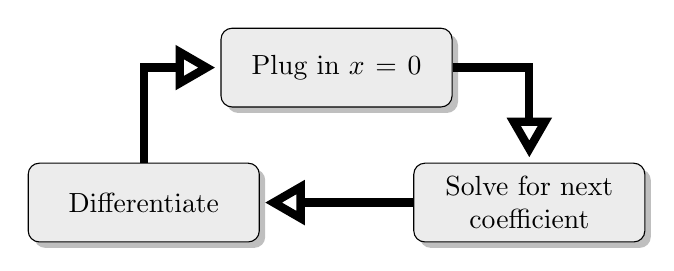
\begin{tikzpicture}[
      >=latex',
      auto
    ]
    
    \tikzstyle{box} = [rectangle, rounded corners, minimum width=2cm, minimum height=1cm, text centered, text width=2.7cm, draw=black, fill=gray!15, drop shadow]
    
    \tikzstyle{arrow} = [thick,>=stealth,arrowhead=5mm,->]
    
    \node [box] (xZero) {
    	Plug in $x=0$
        };
     \node [box]  (solve) [node distance=0.7cm and -.5cm,below right=of xZero] {
     	Solve for next coefficient
     	};
	\node [box]  (diff) [node distance=0.7cm and -0.5cm,below left=of xZero] {
     	Differentiate
     	};
    
    \draw [->, >=open triangle 60, ultra thick,line width= 3pt, shorten >=2pt] (xZero.east) -- ($(xZero.east)+(0.25,0)$) -| (solve.north);
    \draw [->, >=open triangle 60, ultra thick,line width= 3pt, shorten >=2pt] (solve.west) --  (diff.east);
    \draw [->, >=open triangle 60, ultra thick,line width= 3pt, shorten >=2pt] (diff.north) -- ($(diff.north)+(0,0.7)$) |- (xZero.west);

\end{tikzpicture}
	}
    \end{tabular} }
\end{center}

Often this method is called \emph{Taylor's Formula}.  The key idea is to notice that to solve for the coefficient $a_n$, we must differentiate exactly $n$ times and then divide by $n!$.  We rewrite this below in a more formulaic manner. 

\begin{theorem}{\taylorseries{Taylor's Formula}}
If $f(x)$ and all of its derivatives are defined at $x=0$, then 
\begin{align*}
f(x)&=f(0)+f'(0)x+\frac{f''(0)}{2!}x^2+\frac{f'''(0)}{3!}x^3+\cdots \\
  &=\sum_{n=0}^\infty \frac{f^{(n)}(0)}{n!}x^n
\end{align*}
for any value of $x$ for which the sum converges.
\end{theorem}

While the method above works for many functions, it sometimes fails.  In particular, it was no coincidence that the natural logarithm was absent from our examples above!

\begin{exercise}{Natural Log \Coffeecup \Coffeecup}
Try to find a \logarithms{power series} by our brute force method on the function $f(x)=\ln(x)$.  Where does it fail?
\vspace*{2in}
\AnswerKeyEntry{When we try to plug in $x=0$ to find $a_0$, we get $\ln(0)$ which is not a real number.}
\end{exercise}

To work around this, we adopt a more flexible view of power series.  Rather than attempting to write our function as a sum of powers of $x$, which requires the function and its derivatives to be defined at $x=0$, we express it as a sum of powers of $\left(x-a\right)$ for some real number $a$.  It is essentially the same process, but to solve for the coefficients, you would set $x=a$ instead of $x=0$.  This produces a power series \powerseries{centered at $a$}.  We state this method below: 


\begin{center}
\tcbox[left=0mm,right=0mm,top=0mm,bottom=0mm,boxsep=0mm,toptitle=0.5mm,bottomtitle=0.5mm,center title,title=Finding a Power Series Centered at $a$]{\renewcommand*{\arraystretch}{1.8}%
\begin{tabular}{l}
       To find a power series centered at $a$ for a function $f(x)$, carry out the following steps: \\

\textbullet Write down the form of an unknown power series centered at $a$. \\
       $f(x)=a_0+a_1(x-a)+a_2(x-a)^2+a_3(x-a)^3+a_4(x-a)^4+\cdots $ \\
\textbullet Plug in $x=a$ to solve for $a_0$. \\
\textbullet Differentiate both sides and plug in $x=a$ to solve for $a_1$. \\
\textbullet Differentiate both sides and plug in $x=a$ to solve for $a_2$. \\
\textbullet Repeat this until you have as many terms as you need! \vspace*{0.5cm} \\
	\multicolumn{1}{c}{
		\vspace*{0.5cm}
		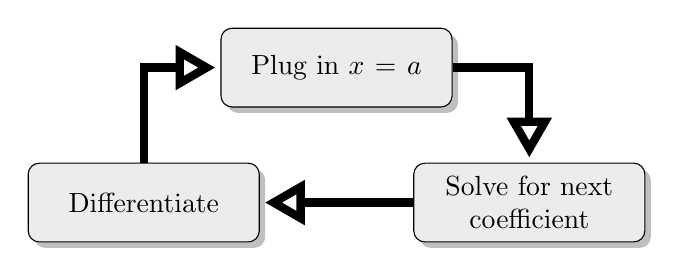
\begin{tikzpicture}[
      >=latex',
      auto
    ]
    
    \tikzstyle{box} = [rectangle, rounded corners, minimum width=2cm, minimum height=1cm, text centered, text width=2.7cm, draw=black, fill=gray!15, drop shadow]
    
    \tikzstyle{arrow} = [thick,>=stealth,arrowhead=5mm,->]
    
    \node [box] (xZero) {
    	Plug in $x=a$
        };
     \node [box]  (solve) [node distance=0.7cm and -.5cm,below right=of xZero] {
     	Solve for next coefficient
     	};
	\node [box]  (diff) [node distance=0.7cm and -0.5cm,below left=of xZero] {
     	Differentiate
     	};
    
    \draw [->, >=open triangle 60, ultra thick,line width= 3pt, shorten >=2pt] (xZero.east) -- ($(xZero.east)+(0.25,0)$) -| (solve.north);
    \draw [->, >=open triangle 60, ultra thick,line width= 3pt, shorten >=2pt] (solve.west) --  (diff.east);
    \draw [->, >=open triangle 60, ultra thick,line width= 3pt, shorten >=2pt] (diff.north) -- ($(diff.north)+(0,0.7)$) |- (xZero.west);



\end{tikzpicture}
	}
    \end{tabular} }
\end{center}

\begin{exercise}{Natural Log, Again \Coffeecup \Coffeecup}
Use the upgraded brute force method to find a \logarithms{power series} for $f(x)=\ln(x)$ centered at $1$. \vspace*{6in}
\AnswerKeyEntry{The power series centered at one for the natural log is $\ln(x)=\Sigma_{n=1}^\infty\frac
{(-1)^{n+1}}{n}(x-1)^n$.}
\end{exercise}

\subsection{Binomial Series}\label{BuyNoMealSeries}

The next exercise constructs the \binomialseries{binomial series}, an extremely important series in the fields of combinatorics, probability, and statistics.

\begin{exercise}{Binomial Series \Coffeecup \Coffeecup \Coffeecup}
Let $m\in\mathbb{R}$.  A function of the form $$f(x)=\left(1+x\right)^m $$ is called a \emph{binomial}, since it has two terms in the polynomial inside parentheses.  Let us run the brute force method on this function to find its power series, the \emph{binomial series}.     

\begin{itemize}
\item Use the brute force method to find the first five terms in the series.  \vspace*{3in}

\item Since that is cumbersome to write down, we define the \emph{binomial coefficient} ``$m$ choose $n$'' to be the following: 

$$\binom{m}{n}=\frac{m\cdot (m-1) \cdot (m-2) \cdots (m-n+1)}{n!} $$ For example, $\binom{7}{3}=\frac{7\cdot 6\cdot 5}{3!}=35$.

Demonstrate that with this notation, the terms you found via brute force are equivalent to the series $$\left( 1+x\right)^m=\sum_{n=0}^\infty\binom{m}{n}x^n. $$ 

\vspace*{2in}

\end{itemize}

\end{exercise}

\newpage

\begin{exercise}{Understanding Binomial Coefficient Notation \Coffeecup}

In the formula for the binomial coefficient $\binom{m}{n}$, how many numbers are multiplied together in the numerator? \vspace*{1in}

\end{exercise}

Note that $m$ was not restricted to being a whole number.  Since it could be fractional, the binomial series allows us to rewrite radicals as polynomials!  

\begin{example}{Power Series of a Cubed Root}
Suppose we wish to find a degree three power series for the function $$f(x)=\sqrt[3]{1+x}. $$

We apply the Binomial Series with $m=1/3$. Proceeding, we have

\begin{align*}
f(x)&=\sqrt[3]{1+x}\\
&=\sum_{n=0}^\infty\binom{1/3}{n}x^n\\
&=\binom{1/3}{0}+\binom{1/3}{1}x+\binom{1/3}{2}x^2+\binom{1/3}{3}x^3+\cdots \\
&=\frac{1}{0!}+\frac{\left(1/3\right)}{1!}x+\frac{\left(1/3\right)\left(-2/3\right)}{2!}x^2+\frac{\left(1/3\right)\left(-2/3\right)\left(-5/3\right)}{3!}x^3+\cdots \\
&=1+\frac{1}{3}x-\frac{1}{9}x^2+\frac{5}{81}x^3+\cdots. \\
\end{align*}

Thus, the best degree three polynomial approximation of $f(x)$ centered at zero is $$ \sqrt[3]{1+x}\approx 1+\frac{1}{3}x-\frac{1}{9}x^2+\frac{5}{81}x^3.$$
\end{example}

\section{Interval of Convergence}

With power series, be warned that not every infinite series will converge for all values of $x$. 

\begin{exercise}{A Convergent Series \Coffeecup}
Let us consider what happens when we evaluate the power series $$\cos(x)=1-\frac{1}{2!}x^2+\frac{1}{4!}x^4-\frac{1}{6!}x^6+\frac{1}{8!}x^8-\cdots  $$ at $x=1$.

We obtain the claim that $\cos(1)=1-\frac{1}{2!}+\frac{1}{4!}-\frac{1}{6!}+\frac{1}{8!}-\cdots$.  Let us test this numerically, remembering that an infinite series is really just a limit of partial sums.  Calculate decimal representations of the partial sums below.
\begin{center}
\begin{tabular}{|c|c|}\hline
Partial Sum & Decimal Approximation \\ \hline
$1$ & \\
$1-\frac{1}{2!}$ & \\
$1-\frac{1}{2!}+\frac{1}{4!}$ & \\
$1-\frac{1}{2!}+\frac{1}{4!}-\frac{1}{6!}$ & \\
$1-\frac{1}{2!}+\frac{1}{4!}-\frac{1}{6!}+\frac{1}{8!}$ & \\ \hline
\end{tabular}
\end{center}
Does it appear that the partial sums are converging to the true value of $\cos(1)$? \vspace*{1in}

\end{exercise}

\begin{exercise}{A Not-So-Convergent Series \Coffeecup}
Let us consider what happens when we evaluate the power series $$\ln(x)=(x-1)-\frac{1}{2}(x-1)^2+\frac{1}{3}(x-1)^3-\frac{1}{4}(x-1)^4+\frac{1}{5}(x-1)^5-\cdots  $$ at $x=3$.

We obtain the claim that $\ln(3)=2-\frac{1}{2}2^2+\frac{1}{3}2^3-\frac{1}{4}2^4+\frac{1}{5}2^5-\cdots $.  Let us again test this numerically, remembering that an infinite series is really just a limit of partial sums.  Calculate decimal representations of the partial sums below.
\begin{center}
\begin{tabular}{|c|c|}\hline
Partial Sum & Decimal Approximation \\ \hline
$2$ & \\
$2-\frac{1}{2}2^2$ & \\
$2-\frac{1}{2}2^2+\frac{1}{3}2^3$ & \\
$2-\frac{1}{2}2^2+\frac{1}{3}2^3-\frac{1}{4}2^4$ & \\
$2-\frac{1}{2}2^2+\frac{1}{3}2^3-\frac{1}{4}2^4+\frac{1}{5}2^5$ & \\ \hline
\end{tabular}
\end{center}
Does it appear that the partial sums are converging to the true value of $\ln(3)$? \vspace*{1in}

\end{exercise}

\subsection{\interval{Definition} of \powerseries{IOC}}

As you can see, power series expansions may be valid for some values of $x$ but not others.  The set of all the ``good'' $x$-values is called the interval of convergence.

\begin{definition}{Interval of Convergence}
Given a power series, the set of all $x$ values for which the infinite sum converges is called the \emph{interval of convergence} (IOC).  The midpoint of the interval is called the \emph{center} of the IOC and the distance from the center to endpoints is called the \emph{radius}. 
\end{definition}

On the interior of the interval, the power series will not only be convergent, but it will be absolutely convergent. This is of enormous convenience, because it means we are free to rearrange terms and do algebra as we like with our power series.

The fact that such a set is always an interval (as opposed to say just scattered points or a union of two disjoint intervals) is not obvious, but it turns out to be true.  To find the interval of convergence, it is typically easiest to use the Ratio Test.  Since power series always have powers of $x$, these will cancel nicely when we apply the Ratio Test.

\begin{example}{\ratiotest{Interval of Convergence} for Cosine}
Consider again our power series 
$$ \cos(x)=\sum_{n=0}^\infty (-1)^{n}\frac{1}{\left(2n\right)!}x^{2n}$$

Let us apply the Ratio Test to this series.  Our goal is to get the absolute value of the ratios of consecutive terms to be less than 1, in which case we are certain the series converges.

\begin{align*}
\lim_{n \rightarrow \infty}\left| \frac{a_{n+1}}{a_n} \right| &=\lim_{n \rightarrow \infty} \left|\frac{(-1)^{n+1}\frac{1}{\left(2(n+1)\right)!}x^{2(n+1)}}{(-1)^{n}\frac{1}{\left(2n\right)!}x^{2n}} \right| \\
 &=\lim_{n \rightarrow \infty} \left|\frac{x^{2n+2}\left(2n\right)!}{\left(2n+2)\right)!x^{2n}} \right| \\
 &=\lim_{n \rightarrow \infty} \left|\frac{x^{2}\left(2n\right)\left(2n-1\right)\cdots 3\cdot 2 \cdot 1}{\left(2n+2\right)\left(2n+1\right)\left(2n\right)\left(2n-1\right)\left(2n-2\right)\cdots 3\cdot 2 \cdot 1} \right| \\
 &=\lim_{n \rightarrow \infty} \left|\frac{x^{2}}{\left(2n+2\right)\left(2n+1\right)} \right| \\
 &=\left|x^2 \right| \lim_{n \rightarrow \infty} \left|\frac{1}{\left(2n+2\right)\left(2n+1\right)} \right| \\
 &=0\left|x^2 \right| \\
 &=0
\end{align*}
The ratio of consecutive terms, being zero, is always strictly less than one no matter what $x$ is.  Since it converges for every $x$ value, the interval of convergence is $(-\infty, \infty)$.
\end{example}

\begin{exercise}{Careful with Algebra! \Coffeecup}
Annotate each line above. Provide a short phrase indicating the reason each simplification was valid.
\end{exercise}

\begin{exercise}{IOC for Natural Log \Coffeecup \Coffeecup \Coffeecup}
Repeat the process above for the series $$ \ln(x)=\sum_{n=1}^\infty (-1)^{n+1}\frac{1}{n}(x-1)^{n}$$

For what $x$-values is the limit of ratios of consecutive terms less than one?

\vspace*{3in}

\end{exercise}

Notice in the above example, if $x=2$ or $x=0$, the limit of ratios of consecutive terms is equal to 1.  This is the case in which the ratio test gives us no information.  Thus, we must test these series for convergence separately.  We can use any of the tests from Section \ref{conv}.   

\begin{exercise}{Checking \interval{Endpoints} \Coffeecup \Coffeecup }
\begin{itemize}
\item Set $x=2$ in the series $\sum_{n=1}^\infty (-1)^{n+1}\frac{1}{n}(x-1)^{n}$ and test it for convergence/divergence.
\vspace*{1in}
\item Set $x=0$ in the series $\sum_{n=1}^\infty (-1)^{n+1}\frac{1}{n}(x-1)^{n}$ and test it for convergence/divergence.
\vspace*{1in}
\item Explain why the interval of convergence for $\ln(x)=\sum_{n=1}^\infty (-1)^{n+1}\frac{1}{n}(x-1)^{n}$ is $(0,2]$.
\vspace*{1in}
\end{itemize}
\end{exercise}

\subsection{Looking at IOC Graphically}

So far we found two IOC's.  Our series for cosine had IOC $\left(-\infty,\infty\right)$.  Our series for the natural logarithm had IOC $\left(0,2\right]$.  Let us compare these situations graphically!

\begin{exercise}{I See the IOC \Coffeecup \Coffeecup}
\begin{itemize}
\item Sketch the graph of cosine, and on the same axes plot the graphs of $P_n(x)$ for $n=0,1,2,3,4,5$, and 6.  You may use a CAS to help come up with the graphs of the polynomials.
\begin{center}
\includegraphics[scale=0.7]{quadall}
\end{center}
\item Sketch the graph of natural log, and on the same axes plot the graphs of $P_n(x)$ for $n=0,1,2,3,4,5$, and 6.  You may use a CAS to help come up with the graphs of the polynomials.
\begin{center}
\includegraphics[scale=0.7]{quadall}
\end{center}
\item What feature of those graphs shows you the IOC? Explain!
\vspace*{1in}
\end{itemize}
\end{exercise}


\section{Mixed Practice with IOC} 
Recall our general framework for power series.  To find a power series centered at $x=a$ for a function $f(x)$, we write down an equation of the form $$ f(x)=a_0+a_1(x-a)+a_2(x-a)^2+a_2(x-a)^3+a_2(x-a)^4+\cdots$$
and then repeatedly plug in $x=a$ and differentiate in order to solve for the coefficients, one at a time.

Though this method will work to find the coefficients as long as the function and its derivatives exist at $x=a$, there remains the question: for what $x$-values will the infinite series on the right actually converge to the corresponding value of $f(x)$?  In this activity, we investigate this both numerically (just using a table of values) and theoretically (using the ratio test).  We call the set of all $x$-values for which a given series converges the \emph{interval of convergence}.

Here we work through this framework in a variety of examples.

\begin{exercise}{Natural Logarithm \Coffeecup \Coffeecup \Coffeecup}
Start with the function $f(x)=\ln(x)$ and do the following:

\begin{itemize}
\item Set up a power series centered at $a=2$ for $\ln(x)$.  Solve for the degree 2, degree 3, degree 4, degree 5, and degree 6 power series approximations for $\ln(x)$ centered at $2$.  Accomplish this by just repeatedly plugging in $x=2$ and differentiating both sides.  Call these functions $P_2(x), P_3(x), P_4(x),$ and  $P_5(x),$ respectively.
\item Make a small table of values where you list out the values of each of your $P_i$ evaluated at $x=1/2$.  Compare this to the true value of $\ln(1/2)$.  
\item Make a small table of values where you list out the values of each of your $P_i$ evaluated at $x=2$.  Compare this to the true value of $\ln(2)$.
\item Perform the Ratio Test on your series expansion for $\ln(x)$.  For what $x$ would you have a ratio less than one?
\item How do your results of the ratio test compare to the numerical evidence you found above?
\item Notice that there will be two $x$-values that cause the series to have ratio exactly equal to one when Ratio Test is applied.  Since the Ratio Test gives no info in that case, try a different test for each of those two series.  
\item At last, state the power series you came up with and the Interval of Convergence.
\end{itemize}
\end{exercise}

\begin{exercise}{Arctangent \Coffeecup \Coffeecup \Coffeecup}
Start with the function $f(x)=\arctan(x)$ and do the following:

\begin{itemize}
\item Set up a power series centered at $x=0$ for $\arctan(x)$.  Solve for the degree 3, degree 5, degree 7, and degree 9 power series approximations.  Accomplish this by just repeatedly plugging in $x=0$ and differentiating both sides.  Call these functions $P_3(x), P_5(x), P_7(x)$, and $P_9(x),$ respectively.  You may want to use a computer algebra system to help with the messy derivatives that will arise!
\item Make a small table of values where you list out the values of each of your $P_i$ evaluated at $x=1/2$.  Compare this to the true value of $\arctan(1/2)$.  
\item Make a small table of values where you list out the values of each of your $P_i$ evaluated at $x=2$.  Compare this to the true value of $\arctan(2)$.
\item Perform the Ratio Test on your series expansion for $\arctan(x)$.  For what $x$ would you have a ratio less than one?
\item How do your results of the ratio test compare to the numerical evidence you found above?
\item Notice that there will be two $x$-values that cause the series to have ratio exactly equal to one when Ratio Test is applied.  Since the Ratio Test gives no info in that case, try a different test for each of those two series.  
\item At last, state the power series you came up with and the Interval of Convergence.
\end{itemize}
\end{exercise}

\begin{exercise}{Exponential \Coffeecup \Coffeecup \Coffeecup}
Start with the function $f(x)=e^x$ and do the following:

\begin{itemize}
\item Set up a power series centered at $x=0$ for $e^x$.  Solve for the degree 2, degree 3, degree 4, and degree 5 power series approximations.  Accomplish this by just repeatedly plugging in $x=0$ and differentiating both sides.  Call these functions $P_2(x), P_3(x), P_4(x),$ and $P_5(x),$ respectively.
\item Make a small table of values where you list out the values of each of your $P_i$ evaluated at $x=1/2$.  Compare this to the true value of $e^{1/2}$.  
\item Make a small table of values where you list out the values of each of your $P_i$ evaluated at $x=2$.  Compare this to the true value of $e^2$.
\item Perform the Ratio Test on your series expansion for $e^x$.  For what $x$ would you have a ratio less than one?
\item How do your results of the ratio test compare to the numerical evidence you found above?  
\item At last, state the power series you came up with and the Interval of Convergence.
\end{itemize}
\end{exercise}

\begin{exercise}{Cosine \Coffeecup \Coffeecup \Coffeecup}
Start with the function $f(x)=\cos(x)$ and do the following:
\begin{itemize}
\item Set up a power series centered at $x=\pi$ for $\cos(x)$.  Solve for the degree 2, degree 4, degree 6, and degree 8 power series approximations.  Accomplish this by just repeatedly plugging in $x=\pi$ and differentiating both sides.  Call these functions $P_2(x), P_4(x), P_6(x),$ and $P_8(x),$ respectively.
\item Make a small table of values where you list out the values of each of your $P_i$ evaluated at $x=\pi/2$.  Compare this to the true value of $\cos\left(\pi/2\right)$.  
\item Make a small table of values where you list out the values of each of your $P_i$ evaluated at $x=2$.  Compare this to the true value of $\cos(2)$.
\item Perform the Ratio Test on your series expansion for $\cos(x)$.  For what $x$ would you have a ratio less than one?
\item How do your results of the ratio test compare to the numerical evidence you found above?  
\item At last, state the power series you came up with and the Interval of Convergence.
\end{itemize}
\end{exercise}

\begin{exercise}{Square Root \Coffeecup \Coffeecup \Coffeecup}
Start with the function $f(x)=\sqrt{x}$ and do the following:

\begin{itemize}

\item Explain why you can't do a power series centered at zero for $\sqrt{x}$.  ({\bf Hint:} Try it.)
\item Instead, set up a power series centered at $x=1$ for $\sqrt{x}$.  Solve for the degree 2, degree 3, degree 4, degree 5, and degree 6 power series approximations for $\sqrt{x}$ centered at $x=1$.  Accomplish this by just repeatedly plugging in $x=1$ and differentiating both sides.  Call these functions $P_2(x), P_3(x), P_4(x),$ and $P_5(x),$ respectively.
\item Make a small table of values where you list out the values of each of your $P_i$ evaluated at $x=1/2$.  Compare this to the true value of $\sqrt{1/2}$.  
\item Make a small table of values where you list out the values of each of your $P_i$ evaluated at $x=2$.  Compare this to the true value of $\sqrt{2}$.
\item Perform the Ratio Test on your series expansion for $\sqrt{x}$.  For what $x$ would you have a ratio less than one?
\item How do your results of the Ratio Test compare to the numerical evidence you found above?
\item Notice that there will be two $x$-values that cause the series to have ratio exactly equal to one when Ratio Test is applied.  Since the Ratio Test gives no info in that case, try a different test for each of those two series.
\item At last, state the power series you came up with and the Interval of Convergence.
\end{itemize}
\end{exercise}

\begin{exercise}{Reciprocal \Coffeecup \Coffeecup \Coffeecup}
Start with the function $f(x)=\frac{1}{1+x}$ and do the following:

\begin{itemize}
\item Set up a power series centered at $x=0$ for $\frac{1}{1+x}$.  Solve for the degree 2, degree 3, degree 4, and degree 5 power series approximations.  Accomplish this by just repeatedly plugging in $x=0$ and differentiating both sides.  Call these functions $P_2(x), P_3(x), P_4(x)$, and $P_5(x),$ respectively.
\item Make a small table of values where you list out the values of each of your $P_i$ evaluated at $x=1/2$.  Compare this to the true value of $\frac{1}{1+\frac{1}{2}}$.  
\item Make a small table of values where you list out the values of each of your $P_i$ evaluated at $x=2$.  Compare this to the true value of $\frac{1}{1+2}$.
\item Perform the Ratio Test on your series expansion for $\frac{1}{1+x}$.  For what $x$ would you have a ratio less than one?
\item How do your results of the ratio test compare to the numerical evidence you found above?
\item Notice that there will be two $x$-values that cause the series to have ratio exactly equal to one when Ratio Test is applied.  Since the Ratio Test gives no info in that case, try a different test for each of those two series.  
\item At last, state the power series you came up with and the Interval of Convergence.
\end{itemize}
\end{exercise}

\section{New Series from Old}

Although the brute force method is a great starting point, we don't want to have to do that every time we want a power series for a function.  Now that we have a library of known power series to draw from, we wish to manipulate these to construct new series rather than starting from scratch every time.  We have four loose categories for finding new series from old:
\begin{itemize}
\item Substitution
\item Algebra 
\item Differentiation
\item Antidifferentiation
\end{itemize}

\begin{subsection}{Substitution}\label{PowerSeriesSubstitution}  Replacing $x$ in a known series by another expression is often useful.

\begin{example}{Variations on a Theme of Euler}
Suppose we wish to find the power series for the function $f(x)=e^{-2x}$.  We can take our known series for the exponential function, $$e^x=1+x+\frac{1}{2!}x^2+\frac{1}{3!}x^3+\cdots, $$ and substitute $-2x$ for each occurance of $x$.  Proceeding, we have 
\begin{align*}
e^{-2x}&=1+\left(-2x\right)+\frac{1}{2!}\left(-2x\right)^2+\frac{1}{3!}\left(-2x\right)^3+\cdots\\
&=1-2x+\frac{2^2}{2!}x^2-\frac{2^3}{3!}x^3+\cdots\\
&=\sum_{n=0}^\infty\left(-1\right)^n\frac{2^n}{n!}x^n.
\end{align*}\end{example}
\begin{exercise}{Checking Against Brute Force \Coffeecup}
Use the brute force method to find the first four coefficients of the power series for $f(x)=e^{-2x}$.  Confirm they match what we obtained above via substitution. \vspace*{2in}
\end{exercise}
\begin{exercise}{Practice with Substitution \Coffeecup \Coffeecup \Coffeecup}
\begin{itemize}
\item Find a power series and the IOC for $\sin(x-1)$ centered at 1.
\vspace*{1in}
\item Find a power series and the IOC for $\sin(2x)$ centered at 0.
\vspace*{1in}
\end{itemize}
\AnswerKeyEntry{If we substitute $x-1$ for $x$ in the power series for sine, we get  $\sin(x-1)=\Sigma_{n=0}^\infty (-1)^{n}\frac{1}{\left(2n+1\right)!}(x-1)^{2n+1}$.  Likewise, substituting $2x$ for $x$ in the power series for sine produces $\sin(2x)=\Sigma_{n=0}^\infty (-1)^{n}\frac{1}{\left(2n+1\right)!}(2x)^{2n+1}=\Sigma_{n=0}^\infty (-1)^{n}\frac{2^{2n+1}}{\left(2n+1\right)!}x^{2n+1}$.}
\end{exercise}

\begin{example}{Revisiting the Arc Length of a Hyperbola}
The binomial series gives us a method by which we can obtain a decimal approximation for the arc length of a hyperbola, as stated in Example \ref{ArcLength}.\ref{HyperBocaBola}.  In that example, we wished to compute 
the arc length of $$y=f(x)=\frac{1}{x}. $$ between $x=\frac{1}{2}$ and $x=1$.  Unfortunately, the arc length integral came out to the less than cooperative  $$L= \int_{x=1/2}^{x=1} \sqrt{1+\left( f'(x)\right)^2 } \dif x= \int_{x=1/2}^{x=1} \frac{\sqrt{1+x^4}}{x^2} \dif x. $$

The trick here is to rewrite the function $\sqrt{1+x^4}$ using the Binomial Series.  In this case, $m=1/2$ and the usual $x$ in the Binomial Series has $x^4$ substituted in.  Proceeding, we see that \begin{align*}
\sqrt{1+x^4}&=\left(1+x^4\right)^{1/2}\\
&=\binom{1/2}{0}+\binom{1/2}{1}\left(x^4\right)+\binom{1/2}{2}\left(x^4\right)^2+\binom{1/2}{3}\left(x^4\right)^3+\binom{1/2}{4}\left(x^4\right)^4+\cdots \\
&=1+\frac{\left(\frac{1}{2}\right)}{1!}x^4+\frac{\left(\frac{1}{2}\right)\left(-\frac{1}{2}\right)}{2!}x^8+\frac{\left(\frac{1}{2}\right)\left(-\frac{1}{2}\right)\left(-\frac{3}{2}\right)}{3!}x^{12}+\frac{\left(\frac{1}{2}\right)\left(-\frac{1}{2}\right)\left(-\frac{3}{2}\right)\left(-\frac{5}{2}\right)}{4!}x^{16}+\cdots \\
&=1+\frac{1}{2}x^4-\frac{1}{8}x^8+\frac{1}{16}x^{12}-\frac{5}{128}x^{16}+\cdots. \\
\end{align*}
Noticing that the $x$-values in the integral are all between $\frac{1}{2}$ and 1, the quantity $x^4$ will also be in that interval.  Since the IOC of the Binomial Series at $m=1/2$ is $[-1,1]$, it is safe to use the power series as a substitute for $\sqrt{1+x^4}$ in the integral.  We now evaluate the integral using the Binomial Series.
\begin{align*}
L&= \int_{x=1/2}^{x=1} \frac{\sqrt{1+x^4}}{x^2} \dif x \\
&=\int_{x=1/2}^{x=1} \frac{1+\frac{1}{2}x^4-\frac{1}{8}x^8+\frac{1}{16}x^{12}-\frac{5}{128}x^{16}+\cdots}{x^2} \dif x \\
&=\int_{x=1/2}^{x=1} \frac{1}{x^2}+\frac{1}{2}x^2-\frac{1}{8}x^6+\frac{1}{16}x^{10}-\frac{5}{128}x^{14}+\cdots \dif x \\
&=\left. -\frac{1}{x}+\frac{1}{2\cdot 3}x^3-\frac{1}{8\cdot 7}x^7+\frac{1}{16\cdot 11}x^{11}-\frac{5}{128\cdot 15}x^{15}+\cdots\right]_{x=1/2}^{x=1}\\
 &=\left(-1+\frac{1}{6}-\frac{1}{56}+\frac{1}{176}-\frac{5}{1920}+\cdots\right)-\left(-2+\frac{1}{6\cdot 2^3}-\frac{1}{56\cdot 2^7}+\frac{1}{176\cdot 2^{11}}-\frac{5}{1920\cdot 2^{15}}+\cdots\right)\\
 &\approx 1.13
\end{align*}
Note this approximation is computed by just adding the terms written above and throwing away all further terms!  
\end{example}

\begin{exercise}{Comparing Two Approximations \Coffeecup}
In the above example, we approximated the arc length of the section of the hyperbola by using finitely many terms from the Binomial Series.  How does it compare if you instead approximated that same arc length via a single line segment?

\vspace*{1in}
\end{exercise}

\end{subsection}

\begin{subsection}{Algebra} An enormous plethora of algebraic tricks are useful with regards to \partialfractions{finding power series} for functions.  Often one can get a lot of mileage out of just factoring and juggling constants.

\begin{example}{Variation on a Geometric Series}
Suppose we wish to find a power series for the function $f(x)=\frac{1}{1-x}$ centered at 3.  We begin by adding and subtracting 3 from $x$, and then proceed to get the geometric series in a form where we can use substitution. \begin{align*}
f(x)&=\frac{1}{1-x}\\
&=\frac{1}{1-\left(x-3+3\right)}\\
&=\frac{1}{1-\left(x-3\right)-3}\\
&=\frac{1}{-2-\left(x-3\right)}\\
&=\frac{1}{-2}\frac{1}{1+\frac{\left(x-3\right)}{2}}\\
&=-\frac{1}{2}\frac{1}{1-\left(-\frac{\left(x-3\right)}{2}\right)}\\
\end{align*}
The motivation for the steps above was to get the series in a form where we can now use substitution into the standard geometric series. Specifically, we substitute $\left(-\frac{\left(x-3\right)}{2}\right)$ in for every occurrence of $x$.  
\begin{align*}
f(x)&=-\frac{1}{2}\left(1+\left(-\frac{\left(x-3\right)}{2}\right)+\left(-\frac{\left(x-3\right)}{2}\right)^2+\left(-\frac{\left(x-3\right)}{2}\right)^3+\cdots\right) \\
&=-\frac{1}{2}+\frac{1}{2^2}\left(x-3\right)-\frac{1}{2^3}\left(x-3\right)^2+\frac{1}{2^4}\left(x-3\right)^3-\cdots.
\end{align*}

\begin{center}
	\includegraphics[width=300px]{ChapterPowerSeries/Figures/IntofConverg}
\end{center}
\end{example}
\begin{exercise}{Checking Against Brute Force \Coffeecup}
Once again, use the brute force method to find the first four coefficients of the power series for $f(x)=\frac{1}{1-x}$ centered at 3.  Confirm they match what we obtained above via algebra and substitution. \vspace*{2in}
\end{exercise}

\begin{exercise}{Practice with Algebra \Coffeecup \Coffeecup \Coffeecup}
\begin{itemize}
\item Find a power series and the IOC for $\frac{1}{x^2-x-12}$ centered at 0. ({\bf Hint:} Use PFD to split into two separate terms, each of which can then be turned into a power series using a variation on the geometric series.)

\vspace*{2in}

\item Find a power series and the IOC for $e^x$ centered at 2. ({\bf Hint:}  Replace $x$ by $(x-2)+2$ and then pull out an $e^2$.)

\vspace*{2in}

\item Find a power series and the IOC for $\sin(x)\cos(x)$ centered at 0. ({\bf Hint:} Avoid taking the nasty product of those two series by applying the sine double angle identity!)

\vspace*{2in}

\item Find a power series and the IOC for $\sin^2(x)$ centered at 0. ({\bf Hint:} Avoid taking the nasty product of sine with itself by applying the sine half angle identity!)

\vspace*{2in}
\item Find a power series and IOC for $\frac{1}{x}$ centered at $5$.

\vspace*{2in}
\end{itemize}
\AnswerKeyEntry{The power series $\frac{1}{x^2-x-12}=\Sigma_{n=0}^\infty  \left(\frac{-1}{21\cdot (-3)^n}-\frac{1}{28\cdot 4^n}\right)x^n$ has IOC (-3,3). The power series $\frac{1}{x}=\Sigma_{n=0}^\infty \frac{(-1)^n}{5^{n+1}}(x-5)^n$ has IOC (0,10).  It turns out these two examples generalize; for rational functions, the IOC will always just be the interval that goes from the center of the series outwards until it bumps into the nearest vertical asymptote!}
\end{exercise}
\end{subsection}

\begin{subsection}{Differentiation}  Often we differentiate a known \deriv{power series term-by-term} to find a new series.
\begin{exercise}{Practice with Differentiation \Coffeecup \Coffeecup \Coffeecup}
\begin{itemize}
\item Find a power series and IOC for $\frac{1}{x^2}$ centered at $5$. ({\bf Hint:} Use the answer from the last problem.)
 
\vspace*{2in}

\item Find a power series and IOC for $\frac{1}{x^3}$ centered at $5$. ({\bf Hint:} Use the answer from the last problem.)

\vspace*{2in}

\item Take the term-by-term derivative of the power series for $e^x$ centered at 0.  Verify that you do in fact get $e^x$ back!

\vspace*{2in}

\end{itemize}
\end{exercise}
\end{subsection}

\begin{subsection}{Antidifferentiation} Often we antidifferentiate a \antider{power series} term-by-term to \integ{find a new power series}.  You will have a ``$+C$'' to solve for by plugging in the center for $x$ after taking the antiderivative.  Notice that this $C$ is really just $a_0$, and plugging in the center for $x$ is just the first step of the brute force method. 

\begin{exercise}{Practice with Antidifferentiation \Coffeecup \Coffeecup \Coffeecup}
\begin{itemize}
\item Take the term-by-term antiderivative of the power series for $e^x$ centered at 0.  Verify that you do in fact get $e^x$ back!

\vspace*{2in}

\item Find a power series and IOC for $\ln(1-x)$ centered at zero.

\vspace*{2in}

\end{itemize}
\AnswerKeyEntry{Antidifferentiate the geometric series to sneak up on $\ln(1-x)$.}
\end{exercise}
\end{subsection}

\begin{exercise}{Four Different Methods for Finding the Same Power Series \Coffeecup \Coffeecup }
Compute the power series for the function $$f(x)=\frac{1}{(1-x)^2} $$
by following the four different methods outlined below:
\begin{enumerate}
\item Finding a power series using differentiation! \begin{itemize}
\item Write out the power series for $\frac{1}{1-x}$.
\item Differentiate both sides.
\vspace*{3in}
\end{itemize}

\item Finding a power series by multiplying together two known series! \begin{itemize}
\item Write out the power series for $\frac{1}{1-x}$.
\item Square both sides.  Note that this will involve a gigantic infinite FOIL on the right-hand side!
\vspace*{3in}
\end{itemize}

\item Finding a power series using long division! \begin{itemize}
\item Expand the denominator of $f(x)$, rewriting our function as $f(x)=\frac{1}{1-2x+x^2}$. 
\item Perform polynomial long division using the lowest degree term on each step to identify your quotient.
\vspace*{3in}
\end{itemize}

\item Finding a power series via brute force! \begin{itemize}
\item Write a general unknown series $f(x)=a_0+a_1x+a_2x^2+a_3x^3+\cdots$. 
\item Plug in zero and differentiate to repeatedly solve for the coefficients one at a time (our brute force method).
\vspace*{3in}
\end{itemize}
\AnswerKeyEntry{Each method should lead to $$\frac{1}{(1-x)^2}=1+2x+3x^2+4x^3+5x^4+\cdots  $$}
\end{enumerate}

\end{exercise}
\section{\taylorseries{Error Bounds}}

Here we state a theorem (without proof) regarding just how accurate a finite degree polynomial approximation is.  It is commonly named after Brook Taylor, who stated it in the 1700s, however Cauchy was the first to actually prove it, roughly 100 years later!

\begin{theorem}{\errorbounds{Taylor's Error Theorem}}
Let $f(x)$ be a function, $n$ a natural number, and $P_n(x)$ the degree $n$ \remainder{power series approximation} centered at a real number $a$. Let $M$ be an upper bound for $\left|f^{(n+1)}(z)\right|$ where $z$ is any number between $x$ and $a$.  Then the error (also called the remainder) in the approximation $$f(x)\approx P_n(x) $$ is no worse than the quantity $$\frac{M|x-a|^{n+1}}{(n+1)!} $$

That is, $$\left| f(x)- P_n(x)\right|\leq \frac{M|x-a|^{n+1}}{(n+1)!} $$
\end{theorem}

Note that in the above theorem, the expression $f^{(n+1)}$ represents $n+1$ derivatives applied to the function $f$.  It is not an exponent.  Notice also that we can be a bit careless when choosing a value of $M$.  If $M$ is exactly the max value of $f^{(n+1)}$ between $x$ and $a$, that will give us the tightest error bound.  Often, for simplicity's sake, we will intentionally choose a $M$ value that is a bit too large.  This still provides a valid error bound, just not one that is as tight as it could have been.  

\begin{example}{\powerseries{Taylor's Error Theorem} Applied to Sine}
Suppose we wish to compute $\sin(0.1)$ \emph{by hand}!  Here is a feasible approach.

\begin{wrapfigure}{r}{0.4\textwidth}
    	\centering
		\includegraphics[height=150px]{ChapterPowerSeries/Figures/ErrorSine}
\end{wrapfigure}

Consider the third degree polynomial approximation $P_3(x)$ of sine, centered at zero.  We have that for $x$ values near zero, $$\sin(x)\approx x-\frac{1}{6}x^3. $$

Suppose we wish to compute $\sin(0.1)$ \emph{by hand} using this approximation.  We evaluate

\begin{align*}
\sin(0.1)&\approx 0.1-\frac{1}{6}\cdot (0.1)^3 \\
&= 0.1-(0.16666\ldots)\cdot(0.001) \\
&= 0.1-0.00016666\ldots \\
&= 0.099833333\ldots.
\end{align*}

Taylor's Error Theorem allows us to analyze how accurate this approximation is.  We list all the components to plug into the error formula below:
\begin{itemize}
\item The function $f(x)$ is $\sin(x)$, the function that we took the power series approximation of.
\item The value of $n$ is 3, the degree of the polynomial approximation.  Notice though here since the degree four coefficient in the power series for sine is zero.  Thus, $P_3(x)=P_4(x)$, so we can get away with using $n=4$ which will give a better error bound. 
\item The center of the power series, $a$, is zero in this case since we used just powers of $x$, not powers of $x-a$ for some nonzero $a$.
\item The value of $x$ is $0.1$, since that is the input value to the function.
\item The upper bound $M=1$ will suffice, since any derivative of a sine or cosine is again a sine or cosine (plus or minus) and thus has outputs of magnitude less than or equal to one.
\end{itemize}

Plugging all of this information into our error bound, we get that our error is no worse than $$\frac{M|x-a|^{n+1}}{(n+1)!}=\frac{1|0.1-0|^{5}}{(5)!}= (0.000001)\cdot(0.008333\ldots)=0.00000008333\ldots.  $$
This tells us that our approximation of $\sin(0.1)$ is incredibly accurate!  The difference between the true value of $\sin(0.1)$ and our approximation $P_4(0.1)=0.099833333\ldots$ is less than $0.00000008333\ldots$.  Another way to say this is that if we were writing out the digits of $\sin(0.1)$ as a decimal, our approximation would have the correct first seven digits past the decimal point (up to rounding).   
\end{example}

\begin{exercise}{Checking Our Work \Coffeecup}
Compute $\sin(0.1)$ on a calculator or CAS.  Verify that the first seven digits after the decimal are correct, and verify that the difference between the true and approximate values is less than $0.00000008333\ldots$ as claimed. \vspace*{1in}
\end{exercise}

\section{What the Cosine Button on Your Calculator Does}

It is worth noting that the definitions of common non-polynomial functions (roots, logs, trig functions, etc) are often very useful for intuition, understanding, and proving theoretical results.  However, they are often atrocious for practical computation!  For example, consider (in year 1 BC, 1 year Before Computers) trying to compute the quantity $\sqrt{4.1}$.  What are you going to do, guess and check?  Will you play the high-low game? 

What is needed is a method for expressing less computationally tractable functions as polynomials (which can be evaluated using good old arithmetic).  We describe our method below!

$$ \text{To compute } f(x) \text{ for a non-polynomial function } f:$$

\begin{enumerate}

\item Find a power series expansion for $f$, preferably centered near $x$.

\item Take a finite degree approximation to this power series (or if the full power series is too difficult to obtain, maybe only compute finitely many terms in the first place).

\item Plug the value for $x$ into your finite degree approximation.

\item Use Taylor's Error Theorem to be sure that your approximation is sufficiently accurate for your purposes.

\end{enumerate}
 
This is the idea behind calculators and computer programs that can so efficiently compute so many wacky functions.  Let's try it by hand together a bit to get a feel for the method.

\begin{exercise}{Seeing Taylor's Error Theorem on a Graph \Coffeecup \Coffeecup}
\begin{itemize}
\item What is the degree 2 power series for $\cos(x)$ centered at zero?  Write the function and plot the graph of both cosine and this parabolic approximation.

\begin{center}
\includegraphics[scale=0.5]{quadall}
\end{center}

\item On your graph, label $y$-coordinates for both functions (cosine and the parabolic approximation) at $x=1$.  What is the gap between the two $y$-coordinates at $x=1$?  That is, how far is the true value of $\cos(1)$ from the estimated value using the degree two polynomial approximation for cosine?  (This gap is what we refer to as the error.)  

\item Apply Taylor's Error Theorem to this situation.  What bound does it give on the error for approximating $\cos(1)$ via the degree two power series centered at zero?  How does this relate to your measurement of the error above?

\vspace*{2in}

\item Suppose we had a calculator that displays ten digits on the screen.  What degree power series \emph{would} you need to guarantee ten digits of accuracy in computing $\cos(1)$?  Show explicitly how you used Taylor's Error Theorem to get your result. ({\bf Hint:} Since any derivative of cosine will just again be plus or minus cosine or sine, you can take $M=1$.)

\vspace*{2in}

\end{itemize}
\end{exercise}

\begin{exercise}{The Error in a Square Root Calculation \Coffeecup \Coffeecup \Coffeecup}
Suppose we wish to compute the number $\sqrt{4.1}$. 
\begin{itemize}
\item Compute a degree one power series for the function $f(x)=\sqrt{x}$ centered at $x=4$.
\vspace*{1in}
\item Plug 4.1 into your degree one power series to get an approximation for $\sqrt{4.1}$. (Note that this is \emph{exactly} what you did in Calc 1 when you looked at tangent lines and linearization as an approximation tool.  The only difference here is we're not stuck at degree 1; we can crank up the degree as much as we like to improve accuracy!)
\vspace*{1in}
\item Compute a degree two power series for the function $f(x)=\sqrt{x}$ centered at $x=4$.
\vspace*{1in}
\item Plug 4.1 into your degree two power series to get an approximation for $\sqrt{4.1}$. 
\vspace*{1in}
\item Compute a degree three power series for the function $f(x)=\sqrt{x}$ centered at $x=4$.
\vspace*{1in}
\item Plug 4.1 into your degree three power series to get an approximation for $\sqrt{4.1}$. 
\vspace*{1in}
\item Apply Taylor's Error Theorem in all three cases above, the degree one, two, and three cases.  How many digits of accuracy do we get in each case?
\vspace*{3in}
\end{itemize}
\AnswerKeyEntry{If $n=1$, we have the following degree one power series centered at $a=4$: $$f(x)=\sqrt{x}\approx 2+\frac{1}{4}(x-4)$$ Since $n=1$, we need the second derivative.  We compute $\left|f''(x)\right|=\frac{1}{4x^{3/2}}$, which on the interval [4,4.1] has its maximum at $x=4$.  Thus, $M=1/32$, which provides an error bound of $$\frac{\frac{1}{32}\cdot|4-4.1|^2}{2!}=\frac{1}{6400}$$  Thus the error is definitely less than one thousandth, but not necessarily less than one ten thousandth.  So for the approximation $$\sqrt{4.1}\approx 2+\frac{1}{4}(4.1-4)=2.025$$ we can guarantee three digits past the decimal are correct but not necessarily the fourth.  That is, 2.025 is certainly the correct decimal expansion for $\sqrt{4.1}$ rounded to the thousandths place.  However, the digit 0 we implicitly have in the ten-thousandths place may or may not be correct.
This process can be repeated for the other $n$ values of two and three.}
\end{exercise}


\begin{exercise}{Clear-Cut Logging \Coffeecup \Coffeecup \Coffeecup}

Compute $\ln(0.9)$ \emph{by hand} accurate to three decimal places.  Really.  Just by hand.  Show all work (including all arithmetic!) below.  ({\bf Hint:} Use Taylor's Error Theorem to make sure you aren't working harder than you need and accidentally using too many terms in the power series.)  

\vspace*{4in}

\end{exercise}

It is worth noting that for most of the history of mathematics, logarithms were computed in essentially this manner, by hand, and then stored in massive tables which then people would use to look them up.  A particularly successful 19th Century French mathematician Gaspard de Prony led a group which compiled a table of logarithms of integers between 1 and 200,000 accurate to 19 decimal places!  His name is one of only 72 engraved onto the Eiffel Tower.

\begin{exercise}{You're Still Smarter Than the Machines \Coffeecup \Coffeecup \Coffeecup}
Complete the following entirely by hand with no calculator use whatsoever! 
\begin{itemize}
\item  Compute $ \sqrt[3]{1001}$ by using a degree two power series approximation for the function $f(x)=\sqrt[3]{x}$ centered at $a=1000$.

\vspace*{2in}

\item  How many digits of accuracy does Taylor's Error Theorem guarantee in this case?

\vspace*{2in}

\end{itemize}
\end{exercise}
\section{Graphing \graphing{Using Power Series}}
\subsection{Second Derivative Test via Power Series}
Recall the Second Derivative Test from Calculus I.  
\begin{exercise}{Go Ahead, Recall It \Coffeecup}
State the Second Derivative Test. \vspace*{1in}
\end{exercise}

How does this relate to looking at the degree two power series of a function?  We investigate below.
\begin{exercise}{\secondderivativetest{Power Series Interpretation} of the Second Derivative Test \Coffeecup \Coffeecup}
Let $c$ be a critical point of the function $f(x)$. 
\begin{itemize}
\item If $f''(c)<0$, what does that tell you about the \concavity{degree two power series} for $f(x)$ centered at $c$? Explain. \vspace*{1in}
\item If $f''(c)>0$, what does that tell you about the degree two power series for $f(x)$ centered at $c$? Explain.  \vspace*{1in}
\item When $f''(c)=0$, in Calculus I we would say the \concavity{Second Derivative Test} gave no information.  With power series, how can you get around this situation and figure out the graph's behavior at that point?  \vspace*{1in}
\end{itemize}
\end{exercise}

Let us now put this to work, analyzing a complicated function!
\begin{exercise}{An Ugly Polynomial \Coffeecup \Coffeecup \Coffeecup}
Graph the function by hand $f(x)=36x-30x^2+\frac{28}{3}x^3-x^4$ using the following steps:

\begin{itemize}
\item Determine the end behavior of the function.  That is, figure out the limits as $x$ approaches infinity and minus infinity.
\vspace*{1in}
\item Compute $f(x)$ at the $x$-values $x=0,2,4,6$ and plot those points to get started.
\vspace*{1in}
\item Compute $f'(x)$ and set it equal to zero to find any critical points.
\vspace*{2in}
\item Find the power series of $f(x)$ centered at each of those critical points.  From these series conclude max/min/saddle at each critical point.  
\vspace*{2in}
\item Sketch the graph!
\begin{center}
\includegraphics[scale=0.5]{quadall}
\end{center}
\end{itemize}
\end{exercise}

\subsection{Symmetry via Power Series}

One powerful technique in mathematics is the exploitation of symmetry.  In the context of graphing, two commonly used types of symmetry are even symmetry and odd symmetry.  Recall the \oddsymmetry{definition}s of even and odd symmetry below.

\begin{exercise}{Definitions of Even and Odd \Coffeecup}
Complete the \evensymmetry{definition}s.
\begin{itemize}
\item We say a function $f(x)$ has \emph{even} symmetry if and only if... \vspace*{.2in}
\item We say a function $f(x)$ has \emph{odd} symmetry if and only if... \vspace*{.2in}
\end{itemize}
\end{exercise}

\begin{exercise}{Symmetry of Sine and Cosine \Coffeecup \Coffeecup}
\begin{itemize}
\item Use the power series for cosine to prove that cosine has \cosine{even symmetry}.
\vspace*{.5in}
\item Use the \oddsymmetry{power series} for sine to prove that sine has \sine{odd symmetry}.
\vspace*{.5in}
\end{itemize}
\AnswerKeyEntry{Substitute $-x$ into the power series for cosine and simplify to demonstrate that $\cos(-x)=\cos(x)$, and similarly for sine.}
\end{exercise}

As the above exercise demonstrates, the key to a function having even (odd) symmetry is for the \evensymmetry{power series} to only have terms of even (odd) degree!  This not only justifies the names of the types of symmetry, but also gives us a quick and easy way to determine the symmetry of a function.  

\begin{exercise}{Testing Our Known Series for Symmetry \Coffeecup \Coffeecup}
Scan through our list of known power series.  Classify each function as odd, even, or neither.  List any symmetries that you found below!
\vspace*{2in}
\end{exercise}

\section{Evaluating Limits Using Power Series}\label{EvalLHR}

Often when faced with an indeterminate form of a limit, it can be resolved by replacing functions with power series.  Specifically, since a limit is trying to study a function as $x$ approaches some value $a$, we use a power series centered at $a$ for the function causing us trouble (or a series centered at whatever value the input is approaching). 

\begin{example}{Evaluating a Limit Using Power Series}
Consider the limit $$\lim_{x \rightarrow \infty} x\sin\left(\frac{1}{x}\right). $$

First, notice this is of the indeterminate form $0\cdot \infty$.  This is a situation we would have typically handled via LHR, but now we have different tools!  As $x$ approaches infinity, $\frac{1}{x}$ approaches zero, so it makes sense to replace sine by its power series centered at zero.  This will allow us to resolve the indeterminate form using ordinary algebra! 

\begin{align*}
\lim_{x \rightarrow \infty} x\sin\left(\frac{1}{x}\right) &=\lim_{x \rightarrow \infty} x\left(\frac{1}{x}-\frac{1}{3!}\frac{1}{x^3}+\frac{1}{5!}\frac{1}{x^5}+\cdots\right) \\
&=\lim_{x \rightarrow \infty} 1-\frac{1}{3!}\frac{1}{x^2}+\frac{1}{5!}\frac{1}{x^4}+\cdots \\
&= 1-\frac{1}{3!}0^2+\frac{1}{5!}0^4+\cdots \\
&=1
\end{align*}
\end{example}

\begin{exercise}{Checking Against LHR \Coffeecup \Coffeecup}
Verify the previous limit calculation using LHR. \vspace*{1in}
\end{exercise}

\begin{exercise}{Practice with Limits via Power Series \Coffeecup \Coffeecup \Coffeecup}

Evaluate each of the following limits two ways:
\begin{enumerate}
\item Using a power series centered at the $x$ value that $x$ is approaching. 

\item Via L'Hospital's Rule.
\end{enumerate}

\begin{itemize}

\item $ \lim_{x\rightarrow 0} \frac{1-\cos(x)}{x}$

\vspace*{1in}

\item $ \lim_{x\rightarrow 0} \frac{1-\cos(x)}{x^2}$

\vspace*{1in}

\item $ \lim_{x\rightarrow 1} \frac{\ln(x)}{x-1}$

\vspace*{1in}

\item $ \lim_{x\rightarrow 1} \frac{\ln(x)}{(x-1)^2}$

\vspace*{1in}

\end{itemize}
\end{exercise}


We at last have the tools to revisit Exercise \ref{LCTomato}.\ref{rabbit} and show where the rabbit came from.

\begin{example}{Cosine of Reciprocals}
Once again, consider the series $\sum_{n=1}^\infty \left(1-\cos\left(\frac{1}{n}\right)\right)$. 
Our rabbit was the decision to compare to the series $\sum_{n=1}^\infty\frac{1}{n^2}$.  This decision was not actually arbitrary, but in fact motivated by power series!  As $n$ approaches $\infty$, the quantity $\frac{1}{n}$ approaches zero.  Thus, it makes sense to replace $\cos\left(\frac{1}{n}\right)$ by its power series centered at zero.  Specifically, we have 

\begin{align*}
1-\cos\left(\frac{1}{n}\right)&=1-\left(1-\frac{1}{2!}\left(\frac{1}{n}\right)^2+\frac{1}{4!}\left(\frac{1}{n}\right)^4-\frac{1}{6!}\left(\frac{1}{n}\right)^6+\cdots\right)\\ 
&=\frac{1}{2!}\frac{1}{n^2}-\frac{1}{4!}\frac{1}{n^4}+\frac{1}{6!}\frac{1}{n^6}+\cdots\\ 
\end{align*}

This power series expansion motivates the choice of $\frac{1}{n^2}$ as comparison function, as it is the dominant term in the expression above.  For large $n$, all other terms are insignificant in comparison.   


We again demonstrate the summands have the same growth order by taking a limit of their ratios.  This time, instead of doing LHR, we use the above power series expansion.
\begin{align*}
\lim_{n\to\infty}\frac{1/n^2}{1-\cos\left(\frac{1}{n}\right)}&=\lim_{n\to\infty}\frac{1/n^2}{\frac{1}{2!}\frac{1}{n^2}-\frac{1}{4!}\frac{1}{n^4}+\frac{1}{6!}\frac{1}{n^6}+\cdots} \\
&=\lim_{n\to\infty}\frac{\left(1/n^2\right)\cdot n^2}{\left(\frac{1}{2!}\frac{1}{n^2}-\frac{1}{4!}\frac{1}{n^4}+\frac{1}{6!}\frac{1}{n^6}+\cdots\right)\cdot n^2} \\
&=\lim_{n\to\infty}\frac{1}{\frac{1}{2!}-\frac{1}{4!}\frac{1}{n^2}+\frac{1}{6!}\frac{1}{n^4}+\cdots } \\
&=\lim_{n\to\infty}\frac{1}{\frac{1}{2}-0+0-0+\cdots} \\
&=\frac{1}{\frac{1}{2}}\\
&=2.
\end{align*}
\end{example}

\begin{exercise}{An Insignificant Calculation \Coffeecup}
In the above example, we made the claim that for large $n$, the later terms of $$ \frac{1}{2!}\frac{1}{n^2}-\frac{1}{4!}\frac{1}{n^4}+\frac{1}{6!}\frac{1}{n^6}+\cdots$$ are insignificant compared to the term $\frac{1}{2!}\frac{1}{n^2}$.  To check this, fill out the following table of values:

\begin{center}
\begin{tabular}{|c|c|c|c|}\hline  & & & \\
$n$ & $\frac{1}{n^2} $ & $ \frac{1}{n^4} $ & $ \frac{1}{n^6}$ \\  
 & & & \\ \hline
 & & & \\
10 & & & \\
 & & & \\
100 & & & \\ 
& & & \\ \hline
\end{tabular}
\end{center}

\end{exercise}
\begin{exercise}{Now You Too Can Be a Magician \Coffeecup \Coffeecup \Coffeecup}
Determine the convergence or divergence of the following series by using power series to find a suitable comparison function and then applying LCT.
\begin{itemize}
\item $ \sum_{n=1}^\infty\arctan\left(\frac{2}{n}\right)$ \vspace*{1in}
\item $ \sum_{n=1}^\infty\arctan\left(\frac{2}{n^2}\right)$ \vspace*{1in}
\item $ \sum_{n=1}^\infty\arcsin\left(\arctan\left(\frac{2}{n}\right)\right)$ \vspace*{1in}
\end{itemize}
\AnswerKeyEntry{Choices of comparison functions and conclusions are as follows: \textbullet $\frac{1}{n}$, diverges \textbullet $\frac{1}{n^2}$, converges \textbullet $\frac{1}{n}$, diverges. }
\end{exercise}
Also, as promised in Section \ref{LHR}, we provide a LHR \LHR{justification using power series}!

\begin{exercise}{Seeing LHR through a Power Series Lens \Coffeecup \Coffeecup \Coffeecup \Coffeecup}

Here we analyze the case where $f(x)$ and $g(x)$ both are functions with convergent power series expansions at a real number $c$.  Assume also $$\lim_{x \rightarrow c}f(x)=\lim_{x \rightarrow c}g(x)=0.$$  We now write out the power series for each function centered at $c$.

$$ f(x)=a_1(x-c)+a_2(x-c)^2+a_3(x-c)^3+\cdots$$
$$ g(x)=b_1(x-c)+b_2(x-c)^2+b_3(x-c)^3+\cdots$$

If $\lim_{x \rightarrow c}f(x)=\lim_{x \rightarrow c}g(x)=0$ and $b_1\not =0$, then 
 \begin{align*}
  \lim_{x \rightarrow c}\frac{f(x)}{g(x)}&=\lim_{x \rightarrow c}\frac{a_0+a_1(x-c)+a_2(x-c)^2+a_3(x-c)^3+\cdots}{b_0+b_1(x-c)+b_2(x-c)^2+b_3(x-c)^3+\cdots} \\ 
  &=\lim_{x \rightarrow c}\frac{0+a_1(x-c)+a_2(x-c)^2+a_3(x-c)^3+\cdots}{0+b_1(x-c)+b_2(x-c)^2+b_3(x-c)^3+\cdots} \\
  &=\lim_{x \rightarrow c}\frac{(x-c)\left(a_1+a_2(x-c)+a_3(x-c)^2+\cdots\right)}{(x-c)\left(b_1+b_2(x-c)+b_3(x-c)^2+\cdots\right)} \\
  &=\lim_{x \rightarrow c}\frac{a_1+a_2(x-c)+a_3(x-c)^2+\cdots}{b_1+b_2(x-c)+b_3(x-c)^2+\cdots} \\
  &=\frac{a_1}{b_1} \\
  &=\lim_{x \rightarrow c}\frac{a_1+2a_2(x-c)+3a_3(x-c)^2+\cdots}{b_1+2b_2(x-c)+3b_3(x-c)^2+\cdots} \\
  &=\lim_{x \rightarrow c}\frac{f'(x)}{g'(x)}.
  \end{align*} 
\begin{itemize}
\item How can we handle the case where $a_1=b_1=0$?  \vspace*{1in}
\item How can we handle the case where $b_1=0$ but $a_1\not = 0$?  \vspace*{1in}
\item What if $c=\infty$ instead of a real number? \vspace*{1in}
\item What if the indeterminate limit is of the form $\frac{\infty}{\infty}$ instead of $\frac{0}{0}$? \vspace*{1in}
\end{itemize}
\AnswerKeyEntry{If the expression $\frac{f(x)}{g(x)}$ is indeterminate of the form $\frac{\infty}{\infty}$, we can trade it out for the expression $\frac{1/g(x)}{1/f(x)}$, which brings us back to the $\frac{0}{0}$ case.}
\end{exercise}

\section{The Fibonacci Numbers via Power Series}\label{FigAndGnocchiNumbers}

Recall the Fibonacci numbers are the recursively defined sequence given by

\begin{align*}
 F_0&=0 \\ 
F_1&=1 \\ 
F_{n+2}&=F_{n+1}+F_n.
\end{align*}

\begin{exercise}{Listing a Few Terms \Coffeecup}
Use the above recursion to compute the first five Fibonacci numbers.  List these below.
\vspace*{.5in}
\end{exercise}

We now compare these numbers to the coefficients of a particular power series.

\begin{exercise}{Coefficients of a Particular Power Series \Coffeecup \Coffeecup \Coffeecup}
\begin{itemize}
\item Use long division to find the first five coefficients of the power series of the following function:
$$ f(x) = \frac{x}{1-x-x^2}. $$
\vspace*{2in}
\item Whoa.  What do you notice about the Fibonacci numbers vs the coefficients in that power series?
\vspace*{.5in}
\end{itemize}
\end{exercise}

We had a recursively defined sequence and a sequence of power series coefficients.  We now compare these to an explicitly defined sequence.
\begin{exercise}{Really? \Coffeecup \Coffeecup}
Define a sequence $a_n$ via the following explicit formula:

$$a_n = \frac{1}{\sqrt{5}} \left( \left(\frac{1+\sqrt{5}}{2}\right)^n-\left(\frac{1-\sqrt{5}}{2}\right)^n \right).   $$
\begin{itemize}
\item Compute the first five terms of this sequence by simply plugging in $n$ values and crunching numbers on a calculator or CAS.  List your answers below.
\vspace*{1in}
\item What?  Yes, really.  Right?
\vspace*{.5in}
\end{itemize}
\end{exercise}

Ok let's figure out what the heck is going on.  Let the function $f(x)=F_0+F_1x+F_2x^2+F_3x^3+\cdots$.  That is, $f$ is defined to be a function whose power series has the Fibonacci sequence as its coefficients.  This is called the \emph{\fibonacci{generating function}} for the Fibonacci numbers.
\begin{exercise}{Studying the Generating Function \Coffeecup \Coffeecup \Coffeecup}
\begin{itemize}

\item Find a power series for the function $xf(x)$.

\vspace*{.5in}

\item Find a power series for the function $x^2f(x)$.

\vspace*{.5in}
 
\item Use the above to find a power series for the function $f(x)-xf(x)-x^2f(x)$.  

\vspace*{1in}

\item Solve the above equation for $f(x)$ to get $f(x)=\frac{x}{1-x-x^2}$.

\vspace*{.5in}

\end{itemize}
\end{exercise}

We now treat the function $f(x)=\frac{x}{1-x-x^2}$ as a ``New Series from Old'' style exercise.  Once we find a formula its coefficients, we will have a formula for the Fibonacci numbers!

\begin{exercise}{Finding an Explicit Formula for the Coefficients \Coffeecup \Coffeecup \Coffeecup}
\begin{itemize}
\item Factor the polynomial $1-x-x^2$ via the quadratic formula.  In particular, factor into the form $\left(1-\frac{x}{r_1}\right)\left(1-\frac{x}{r_2}\right)$ where $r_1$ and $r_2$ are the roots.
\vspace*{1in}
\item Use this factorization to find the partial fraction decomposition of $f(x)=\frac{x}{1-x-x^2}$.
\vspace*{2in}
\item Use the geometric series formula to find a power series for each term in the PFD, then add them together to get a power series for the \partialfractions{Fibonacci generating function} $f(x)=\frac{x}{1-x-x^2}$. 
\vspace*{3in}
\item Equate the general degree $n$ coefficient with $F_n$ to obtain the above explicit formula for the Fibonacci numbers!
\vspace*{1in}
\end{itemize}
\end{exercise}

The explicit formula for the Fibonacci Numbers is known as \emph{Binet's Formula}.  We state it again here, just because it is so nice to look at.

\begin{theorem}{Binet's Formula} For all $n\in \mathbb{N}$,

$$F_n = \frac{1}{\sqrt{5}} \left( \left(\frac{1+\sqrt{5}}{2}\right)^n-\left(\frac{1-\sqrt{5}}{2}\right)^n \right).   $$

\end{theorem}
\begin{exercise}{Ratio of Consecutive Fibonacci Numbers  \Coffeecup \Coffeecup}

We now revisit Exercise \ref{convseq}.\ref{Fibbies}, armed with Binet's Formula!  Use Binet's Formula to compute the limit of the ratio of consecutive Fibonacci numbers.  That is, compute an exact value for the following limit:

$$\lim_{n\rightarrow \infty}\frac{F_{n+1}}{F_n} \hspace{4in}$$
\vspace*{2in} \AnswerKeyEntry{The ratio between consecutive terms is $\frac{1+\sqrt{5}}{2}$, the Golden Ratio.}
\end{exercise}

\begin{exercise}{IOC \Coffeecup \Coffeecup}
Find the IOC for the Fibonacci generating function.  How does this relate to vertical asymptotes on the graph of $\frac{x}{1-x-x^2}$?
\vspace*{2in} \AnswerKeyEntry{The IOC is $\left(\frac{1-\sqrt{5}}{2},\frac{\sqrt{5}-1}{2}\right)$.  This is the interval that proceeds symmetrically left and right from the origin as far as it can until it runs into the nearest vertical asymptote of $\frac{x}{1-x-x^2}$.}
\end{exercise}
Again armed now with Binet's Formula, we revisit Exercise \ref{AppleCations}.\ref{Lieonacci}.

\begin{exercise}{Sums of Consecutive Fibonacci Numbers \Coffeecup \Coffeecup \Coffeecup}

Use Binet's Formula to verify that a sum of consecutive Fibonacci numbers is in fact always one less than the following Fibonacci number.  That is, show that $$  \sum_{i=0}^n F_i = F_{n+1}-1$$ by rewriting the left-hand side summand using Binet's Formula and then summing the geometric series that result.
\vspace*{3in}
\end{exercise}
Here we offer another proof of the same summation identity!  In this argument, we build yet another generating function for the sums of the Fibonacci numbers rather than for the Fibonacci numbers themselves.
\begin{exercise}{Another Take on Sums of Consecutive $F_n$ \Coffeecup \Coffeecup \Coffeecup}
\begin{itemize}
\item By expanding and multiplying power series, demonstrate that the following product is valid: 

$$   \left(\sum_{n=0}^\infty F_nx^n\right)\left(\sum_{n=0}^\infty x^n\right) = \sum_{n=0}^\infty \left( \sum_{i=0}^n F_i \right)x^n. $$

\vspace*{1in}
\item Explain why the left-hand side above is equal to the
function $g(x)=\frac{x}{\left(1-x-x^2\right)\left(1-x\right)}$.

\vspace*{.5in}

\item Verify the PFD $g(x)=\frac{x}{\left(1-x-x^2\right)\left(1-x\right)}=\frac{1+x}{1-x-x^2}-\frac{1}{1-x}$.

\vspace*{.5in}

\item Use that PFD along with our known series for the Fibonacci generating function and the geometric series to show the power series for $g(x)$ has $F_n+F_{n-1}-1$ as its general degree $n$ coefficient for natural numbers $n>0$. 

\vspace*{1in}

\item Conclude that the identity $  \sum_{i=0}^n F_i = F_{n+1}-1$ is true, as both the left- and right-hand sides represent the degree $n$ coefficient of $g(x)$.

\vspace*{.5in}

\end{itemize}
\end{exercise}


\section{Evaluating Infinite Sums Using Power Series}

In Section \ref{conv}, we developed many ways to determine if an infinite series converges, but we had almost no methods for determining what value a series converges to.  Unless the series was geometric or telescoping, we were stuck.  Armed with our list of power series, we have much better tools!  Given an infinite series we wish to evaluate, we can now do the following:

\begin{itemize}
\item Look for key identifying features of the series that remind us of some known power series.
\item See what $x$-value we can plug into our known power series to obtain the infinite series (or something close enough to it).
\item Check that $x$-value was in the IOC of the power series, to be sure we were using a valid input.
\end{itemize}

\begin{example}{Evaluating an Infinite Series}
Consider the infinite series $$ -\frac{3}{2!}+\frac{3^2}{3!}-\frac{3^3}{4!}+\frac{3^4}{5!}-\frac{3^5}{6!}+\cdots. $$

We can convince ourselves that it converges using the Ratio Test.  But what value does it converge to?  We begin by noticing the similarity to the power series for $e^x$ based on the consecutive factorials in the denominator.  We then notice the ascending powers of 3 and the alternating signs in the infinite sum; this motivates $x=-3$ as a good choice for input.  We write this infinite series down and then play with the equation until we obtain the infinite series above.  In particular,
$$e^{-3}=1-\frac{3}{1!}+\frac{3^2}{2!}-\frac{3^3}{3!}+\frac{3^4}{4!}-\frac{3^5}{5!}+\cdots. $$ 
Notice that the powers of three in our infinite sum are one less than the corresponding factorial, and the signs are off.  Dividing both sides by negative three fixes this.
$$-\frac{1}{3}e^{-3}=-\frac{1}{3}+\frac{1}{1!}-\frac{3^1}{2!}+\frac{3^2}{3!}-\frac{3^3}{4!}+\frac{3^4}{5!}-\cdots $$
The first two terms can be moved over to left-hand side. $$-\frac{1}{3}e^{-3}+\frac{1}{3}-\frac{1}{1!}=-\frac{3}{2!}+\frac{3^2}{3!}-\frac{3^3}{4!}+\frac{3^4}{5!}-\cdots $$
We combine those terms with arithmetic, and we have our total for the infinite series!
 $$-\frac{3}{2!}+\frac{3^2}{3!}-\frac{3^3}{4!}+\frac{3^4}{5!}-\cdots=-\frac{1}{3}e^{-3}-\frac{2}{3} $$
\end{example}

\begin{exercise}{Checking with Ratio Test and Some Numerics \Coffeecup}

\begin{itemize}
\item In the above example, it is claimed that the series converges by the Ratio Test.  Verify by applying the Ratio Test and showing all details of the computation below.
\vspace*{2in}
\item Evaluate $-\frac{1}{3}e^{-3}-\frac{2}{3}$ in a calculator or CAS.  Compute a large partial sum of terms from the infinite series and verify that the answer is reasonable.  (A quick numeric check like this is very valuable for catching minus sign mistakes or other algebra errors!)
\vspace*{1in}
\end{itemize}
\end{exercise}

Ok, try a few!

\begin{exercise}{Evaluating Infinite Series Using Power Series \Coffeecup \Coffeecup \Coffeecup} Evaluate each of the following to a number in closed form.  Or, if the series does not converge, simply say ``diverges'' and give a brief explanation why.

\begin{itemize}
\item $1-\frac{1}{2}+\frac{1}{3}-\frac{1}{4}+\frac{1}{5}-\cdots$

\vspace*{.9in}

\item $1-\frac{1}{2!}+\frac{1}{3!}-\frac{1}{4!}+\frac{1}{5!}-\cdots$
\vspace*{.9in}

\item $3-\frac{3}{2!}+\frac{3}{3!}-\frac{3}{4!}+\frac{3}{5!}-\cdots$
\vspace*{.9in}

\item $3-\frac{3^2}{2!}+\frac{3^3}{3!}-\frac{3^4}{4!}+\frac{3^5}{5!}-\cdots$
\vspace*{.9in}

\item $3-\frac{3^2}{2}+\frac{3^3}{3}-\frac{3^4}{4}+\frac{3^5}{5}-\cdots$
\vspace*{.9in}

\item $1-\frac{1}{2}+\frac{1}{3\cdot 2}-\frac{1}{4\cdot 3}+\frac{1}{5\cdot 4}-\cdots$
\vspace*{.9in}

\item $6+\frac{6}{4}+\frac{6}{9}+\frac{6}{16}+\frac{6}{25}+\cdots$

\vspace*{.9in}

\item $\binom{40}{0}+\binom{40}{1}+\binom{40}{2}+\binom{40}{3}+\binom{40}{4}+\cdots $

\vspace*{.9in}

\item $\binom{40}{0}-\binom{40}{1}+\binom{40}{2}-\binom{40}{3}+\binom{40}{4}-\cdots $

\vspace*{.9in}

\end{itemize}
\end{exercise}

Notice also that if you simply skip the step of plugging in a number for $x$, you can often evaluate a power series to a closed form.  This will be particularly useful in Chapter \ref{diffeq}.

\begin{exercise}{Finding Closed Forms for Power Series \Coffeecup \Coffeecup \Coffeecup}
Evaluate each of the following into a closed form.
\begin{itemize}

\item $5x-\frac{5}{2!}x^2+\frac{5}{3!}x^3-\frac{5}{4!}x^4+\frac{5}{5!}x^5-\cdots$

\vspace*{2in}

\item $-\frac{5}{2!}x^2+\frac{5}{3!}x^3-\frac{5}{4!}x^4+\frac{5}{5!}x^5-\cdots$

\vspace*{2in}

\item  $1+5x-\frac{5^2}{2!}x^2+\frac{5^3}{3!}x^3-\frac{5^4}{4!}x^4+\frac{5^5}{5!}x^5-\cdots$

\vspace*{2in}

\item  $5+5^2x-\frac{5^3}{2!}x^2+\frac{5^4}{3!}x^3-\frac{5^5}{4!}x^4+\frac{5^6}{5!}x^5-\cdots$

\vspace*{2in}

\item  $5+5^2x-\frac{5^3}{2!}x^2-\frac{5^4}{3!}x^3+\frac{5^5}{4!}x^4+\frac{5^6}{5!}x^5-\frac{5^7}{6!}x^6-\frac{5^8}{7!}x^7\cdots$

\vspace*{2in}

\item  $5x+5^2x^2-\frac{5^3}{2!}x^3-\frac{5^4}{3!}x^4+\frac{5^5}{4!}x^5+\frac{5^6}{5!}x^6-\frac{5^7}{6!}x^7-\frac{5^8}{7!}x^8\cdots$

\vspace*{2in}
\end{itemize}
\end{exercise}

\begin{exercise}{Converting Back and Forth \Coffeecup \Coffeecup \Coffeecup}
For each of the following series, convert it into a closed form $f(x)$.  Afterwards, find a power series centered at 1 for the function you came up with and verify that it matches the original series.
\begin{itemize}
\item $\sum_{n=0}^\infty (x-1)^n $
\vspace*{1in}
\item $\sum_{n=0}^\infty \binom{1/2}{n}(x-1)^n $
\vspace*{1in}
\item $\sum_{n=1}^\infty \frac{1}{n}(x-1)^n $
\vspace*{1in}
\item $\sum_{n=0}^\infty (-1)^n(x-1)^n $
\vspace*{1in}
\item $\sum_{n=0}^\infty \frac{1}{(n+1)!}(x-1)^n $
\vspace*{1in}
\end{itemize} \AnswerKeyEntry{\textbullet $\frac{1}{2-x}$ \textbullet $\sqrt{x}$ \textbullet $-\ln(2-x)$ \textbullet $\frac{1}{x} $ \textbullet $\frac{e^{x-1}-1}{x-1}$ }
\end{exercise}

\begin{comment}

We have two forms, closed form functions and their power series.  We also have a way to go back and forth between the two forms.  This calls for another game of... TELEPHONE!

Break into groups of four and play telephone with one of the following pages.  If you are handed an explicit formula for a function $f(x)$, find the power series centered at one for that same function fold over the original $f(x)$, and pass it along.  If you are handed a power series, find the function $f(x)$ it evaluates to, fold over the original power series, and pass it along. 

\newpage

$$\sum_{n=0}^\infty (x-1)^n $$

\hrulefill

\vspace{.5in}

\begin{center}
\fbox{$f(x)=$ \hspace{3in}}
\end{center}

\vspace{.5in}

\hrulefill

\vspace{.5in}

\begin{center}
\fbox{$\sum_{n=0}^\infty$ \hspace{3in}}
\end{center}

\vspace{.5in}

\hrulefill

\vspace{.5in}

\begin{center}
\fbox{$f(x)=$ \hspace{3in}}
\end{center}

\vspace{.5in}

\hrulefill

\vspace{.5in}

\begin{center}
\fbox{$\sum_{n=0}^\infty$ \hspace{3in}}
\end{center}

\vspace{.5in}

\pagebreak

$$\sum_{n=0}^\infty \binom{1/2}{n}(x-1)^n $$

\hrulefill

\vspace{.5in}

\begin{center}
\fbox{$f(x)=$ \hspace{3in}}
\end{center}

\vspace{.5in}

\hrulefill

\vspace{.5in}

\begin{center}
\fbox{$\sum_{n=0}^\infty$ \hspace{3in}}
\end{center}

\vspace{.5in}

\hrulefill

\vspace{.5in}

\begin{center}
\fbox{$f(x)=$ \hspace{3in}}
\end{center}

\vspace{.5in}

\hrulefill

\vspace{.5in}

\begin{center}
\fbox{$\sum_{n=0}^\infty$ \hspace{3in}}
\end{center}

\vspace{.5in}

\pagebreak

$$\sum_{n=0}^\infty \frac{(-1)^n}{n+1}(x-1)^n $$

\hrulefill

\vspace{.5in}

\begin{center}
\fbox{$f(x)=$ \hspace{3in}}
\end{center}

\vspace{.5in}

\hrulefill

\vspace{.5in}

\begin{center}
\fbox{$\sum_{n=0}^\infty$ \hspace{3in}}
\end{center}

\vspace{.5in}

\hrulefill

\vspace{.5in}

\begin{center}
\fbox{$f(x)=$ \hspace{3in}}
\end{center}

\vspace{.5in}

\hrulefill

\vspace{.5in}

\begin{center}
\fbox{$\sum_{n=0}^\infty$ \hspace{3in}}
\end{center}

\vspace{.5in}

\pagebreak

$$\sum_{n=0}^\infty (-1)^n(x-1)^n $$

\hrulefill

\vspace{.5in}

\begin{center}
\fbox{$f(x)=$ \hspace{3in}}
\end{center}

\vspace{.5in}

\hrulefill

\vspace{.5in}

\begin{center}
\fbox{$\sum_{n=0}^\infty$ \hspace{3in}}
\end{center}

\vspace{.5in}

\hrulefill

\vspace{.5in}

\begin{center}
\fbox{$f(x)=$ \hspace{3in}}
\end{center}

\vspace{.5in}

\hrulefill

\vspace{.5in}

\begin{center}
\fbox{$\sum_{n=0}^\infty$ \hspace{3in}}
\end{center}

\vspace{.5in}

\pagebreak

$$\sum_{n=0}^\infty \frac{1}{(n+1)!}(x-1)^n $$

\hrulefill

\vspace{.5in}

\begin{center}
\fbox{$f(x)=$ \hspace{3in}}
\end{center}

\vspace{.5in}

\hrulefill

\vspace{.5in}

\begin{center}
\fbox{$\sum_{n=0}^\infty$ \hspace{3in}}
\end{center}

\vspace{.5in}

\hrulefill

\vspace{.5in}

\begin{center}
\fbox{$f(x)=$ \hspace{3in}}
\end{center}

\vspace{.5in}

\hrulefill

\vspace{.5in}

\begin{center}
\fbox{$\sum_{n=0}^\infty$ \hspace{3in}}
\end{center}

\vspace{.5in}

\end{comment}
\section{Power Series \powerseries{Reference Sheet}}
Here we compile our list of known series.  Write each below, both listing terms and in sigma notation, indicating the center and the interval of convergence in each case (except Binomial which will not fit in that little IOC block): \vspace{.2in}
\begin{center}
\begin{tabular}{|c|c|c|c|} \hline
Function & Series in Sigma Notation & \hspace*{.5in}  Series in Expanded Form \hspace*{.5in} & IOC \\ \hline \hline
& & & \\
& & & \\
Geometric:  & & & \\
& & & \\
& & & \\
& & & \\
& & & \\
Exponential:  & & & \\
& & & \\
& & & \\
& & & \\
& & & \\
Sine:  & & & \\
& & & \\
& & & \\
& & & \\
& & & \\
Cosine:  & & & \\
& & & \\
& & & \\
& & & \\
& & & \\
Natural Log:  & & & \\
& & & \\
& & & \\
& & & \\
& & & \\
Arctangent:  & & & \\
& & & \\
& & & \\
& & & \\
& & & \\
Binomial:  & & &  \\
& & & \emph{Long Story} \\
& & & \\
& & & \\
& & & \\
Fibonacci:  & & & \\
& & & \\
& & & \\
& & & \\\hline
\end{tabular}
\end{center}

\section{Chapter Summary}
In this chapter, we undertook the mission of rewriting the many different types of nonpolynomial functions we have (especially rational, exponential, logarithmic, trigonometric, inverse trigonometric, and radical) as polynomials (usually of infinite degree).
\begin{enumerate}
\item {\bf Building the theory of power series!}  
\begin{enumerate}
\item {\bf Given a function, find its power series centered at $a$:} Given some function $f(x)$, rewrite it as $$f(x)=a_0+a_1(x-a)+a_2(x-a)^2+a_3(x-a)^3+a_4(x-a)^4+\cdots$$
via one of the following methods: \begin{itemize}
\item {\bf Brute force method:}  Repeatedly differentiate the function, plug in $x=a$, and solve for the coefficients one at a time until a pattern appears or you have enough terms for your purposes.
\item {\bf New series from old:} Using a known power series as a starting point and then manipulating via substitution, algebra, differentiation, antidifferentiation, or other valid forms of trickery.
\end{itemize}
\item {\bf Given a power series, find the interval of convergence:} Use the ratio test to find the interior of the interval.  The endpoints then will have to be plugged in one at a time and convergence can be determined using some test other than the ratio test.
\item {\bf Use Taylor's Error Bound to determine the accuracy in approximating functions with finite degree power series:} When trying to compute the value of $f(x)$ via a finite power series approximation, we can obtain an upper bound for the error as follows: $$\left| f(x)- \underset{\text{degree }n\text{ power series for }f(x)\text{ centered at }a}
{\underbrace{\left(a_0+a_1\left(x-a\right)+a_2\left(x-a\right)^2+a_3\left(x-a\right)^3+\cdots+a_n\left(x-a\right)^n\right)}}\right|\leq \frac{M|x-a|^{n+1}}{(n+1)!} $$
where $M$ is an upper bound for the absolute value of the $(n+1)^{\text{st}}$ derivative of $f$ between $a$ and $x$.
\end{enumerate}
\item {\bf Applications of power series!}  There are of course many many many more applications of power series, but we focused on a few in particular.
\begin{enumerate}
\item {\bf Analyzing graphs using power series:} Just as we approximated graphs using tangent lines in Calc I, we can now approximate the shapes of graphs via tangent lines, parabolas, cubics, etc.  $$f(x)=\underset{\underset{\hspace{.5in}\ddots}{\text{approximating cubic at }x=a}}{ \underbrace{\underset{\text{approximating parabola at }x=a}{ \underbrace{\underset{\text{tangent line at }x=a}{\underbrace{\underset{y \text{ coordinate at }x=a}
{\underbrace{a_0}}+a_1\left(x-a\right)}}+a_2\left(x-a\right)^2}}+a_3\left(x-a\right)^3}}+\cdots $$

\item {\bf Evaluate indeterminate forms of limits using power series:} We can justify LHR (or bypass it) by instead replacing functions by power series centered at the value the input is approaching, and then evaluate the limit via algebra.

\item {\bf Evaluate infinite series using power series:}  Given an infinite series, find a closed form (if possible) by identifying a power series it resembles and performing appropriate manipulations (substitutions for $x$, algebra, etc) to make it match.

\end{enumerate}
\end{enumerate}

\section{Mixed Practice}
\subsection{Warm Ups}
These are good problems for reinforcing the vocabulary and foundational concepts of this chapter. 

\begin{exercise}{Reference Sheet \Coffeecup}
Make sure your power series reference sheet is completely filled out.  Once you do, see if you can rewrite it correctly from memory without looking at the original.  It is essential to have those formulas internalized in order to be proficient with power series.
\end{exercise}

\subsection{Sample Test Problems}

\begin{exercise}{\Coffeecup \Coffeecup }
By hand, (or using your custom built Arduino calculator) compute the cubed root of $e$ accurate to one place past the decimal. (That is, error less that one one-tenth)  Use Taylor's error theorem to justify your answer is correct!
\AnswerKeyEntry{$1.4$}
\solushun{Note: $\sqrt[3]{e}= e^{1/3}$ Thus we need to substitute $x= \frac{1}{3} $ into $f(x) = e^{x}= \sum\limits_{n=0}^{\infty}{\frac{x^n}{n!}}$ This means $a=0$.  Also we have $f^{n+1} =e^x$ which has its max at $\frac{1}{3}$ on the interval $[0,\frac{1}{3}]$.  We don't know the value of $e^{1/3}$ since its what we are trying to compute but we can infer the value from the fact that $e<2^3=8$ which means that $e^{1/3} <2$  Therefore we can use $M=2$ as a safe estimator in our error formula.  Thus the error in a degree $n$ approximation will be $\frac{M \cdot |x-a|^{n+1}}{(n+1)!}=\frac{2 \left|\frac{1}{3}-0\right|^{n+1}}{(n+1)!}=\frac{2}{3^{n+1}(n+1)!}$ which we need to be less and 0.1. We can look at this in a table:
\begin{center}
\begin{tabular}{|c|c|} \hline
$n$ & $\frac{2}{3^{n+1}(n+1)!}$  \\ \hline
 1 & $\frac{2}{3^{2}(2)!}=\frac{1}{9} $  \\ 
 2 &  $\frac{2}{3^{3}(3)!} = \frac{1}{81}<\frac{1}{10}$ \\
 3 &  $\frac{2}{3^{4}(4)!} = \frac{1}{972}<\frac{1}{100}$ \\
\end{tabular}
\end{center}
So we use $n=2$ to compute:$e^{1/3} = 1+ \frac{1}{3} + \frac{\left(\frac{1}{3}\right)^2}{2!}= 1+ \frac{1}{3} +\frac{1}{18} = 1+ 0.3333 \dotfill  + 0.05555 \dotfill \approx 1.4$\\}{0in}
\end{exercise}

\begin{exercise}{\Coffeecup \Coffeecup }
 For each of the following, identify whether the sum converges to a real number or if it diverges.  If it converges, find a closed form for the real number it converges to.  You may cite results stated in class or in homework.
\begin{enumerate}[label=\alph*.)]
\item $1+\binom{1/2}{1}+\frac{\left(\binom{1/2}{1}\right)^2}{2!}+\frac{\left(\binom{1/2}{1}\right)^3}{3!}+\frac{\left(\binom{1/2}{1}\right)^4}{4!}+\cdots $
\solushun{$1+\binom{1/2}{1}+\frac{\left(\binom{1/2}{1}\right)^2}{2!}+\frac{\left(\binom{1/2}{1}\right)^3}{3!}+\frac{\left(\binom{1/2}{1}\right)^4}{4!}+\cdots  = 1 + \frac{\left(\frac{1}{2}\right)}{2!}+\frac{\left(\frac{1}{2}\right)^2}{3!}+\frac{\left(\frac{1}{2}\right)^3}{4!}+\cdot = \sum\limits_{n=0}^{\infty} \frac{\left(\frac{1}{2}\right)^{n}}{n!} = e^{1/2}=\sqrt{e}$
\\ }{0in}

\item $1+\binom{1/2}{1}+\binom{1/2}{2}+\binom{1/2}{3}+\binom{1/2}{4}+\cdots $
\solushun{$1+\binom{1/2}{1}+\binom{1/2}{2}+\binom{1/2}{3}+\binom{1/2}{4}+\cdots=
\sum\limits_{n=0}^{\infty}{\binom{1/2}{n} 1^{n}}=(1+1)^{1/2} = \sqrt{2}$
\\ }{0in}

\item $0.20202020202020\ldots$ 
\solushun{$0.20202020202020\ldots= \frac{20}{100} + \frac{20}{10000} + \frac{20}{1000000}+ \cdot = 0.2\left(1+ \frac{1}{100} + \frac{1}{10000} + \frac{1}{1000000}+ \cdot\right) = 0.2\sum_{n=0}^{\infty}{\left(\frac{1}{100}\right)^{n}}$ This is a Geometric Series so $0.2\sum_{n=0}^{\infty}{\left(\frac{1}{100}\right)^{n}}=\frac{2}{10}\cdot \frac{1}{1-\frac{1}{100}}= \frac{2}{10}\frac{100}{99} = \frac{20}{99}$ 
\\ }{0in}

\item $5+5^2/1!+5^3/2!+5^4/3!+5^5/4!+\cdots $
\solushun{$5+5^2/1!+5^3/2!+5^4/3!+5^5/4!+\cdots =5\left(1+5/1!+5^2/2!+5^3/3!+5^4/4!+\cdots\right)= 5 \sum\limits_{n = 0}^{\infty}{\frac{5^n}{n!}} = 5e^5 $
\\ }{0in}
\end{enumerate}
\AnswerKeyEntry{a.) $\sqrt{e}$,~~b.) $\sqrt{2}$,~~c.) $\frac{20}{99}$,~~d.) $5e^5$}

\end{exercise}

\begin{exercise}{\Coffeecup \Coffeecup }
Consider the following limit: 
$$ \lim\limits_{x\rightarrow 0} \frac{x^2}{\sec(x)-1}$$

\begin{enumerate}[label=\alph*.)]
\item Evaluate the limit by L'Hospital's Rule.
\solushun{ $ \lim\limits_{x\rightarrow 0} \frac{x^2}{sec(x)-1} \stackrel{\text{H}}{=} \lim\limits_{x\rightarrow 0} \frac{2x}{\sec{x}\tan{x}} \stackrel{\text{H}}{=} =\lim\limits_{x\rightarrow 0} \frac{2}{\sec{x}\tan^{2}{x}+\sec^3{x}}\frac{2}{0+1} = 2$
\\ }{0in}

\item Evaluate the limit by replacing $\sec(x)$ with its power series centered at zero.  (HINT: You only need a few terms of this series in order to evaluate the limit!)  Verify that your results match.
\solushun{Brute force a degree 2 power series for $\sec{x}=a_0+a_1 x+a_2 x^2$.\\
Set $x=0$ then $\sec{0} = a_0 \longleftrightarrow a_0 = 1$\\
Differentiate: $\sec{x}\tan{x} = a_1+2a_2 x$ Set $x=0\longleftrightarrow 0 = a_1$\\
Differentiate: $\sec{x}\tan^2{x} + \sec^3{x} = 2a_2$ Set $x=0 \longleftrightarrow 0+1 = 2a_2 \longleftrightarrow a_2 = \frac{1}{2}$ thus\\
$\lim\limits_{x\rightarrow 0} \frac{x^2}{sec(x)-1} = \lim\limits_{x\rightarrow 0} \frac{x^2}{1+\frac{1}{2}x^2} = \lim\limits_{x\rightarrow 0} \frac{1}{\frac{1}{x^2}+\frac{1}{2}}= \frac{1}{\frac{1}{2}} = 2$
\\ }{0in}

\end{enumerate}
\AnswerKeyEntry{a.~~ 2 
b.~~ $\lim\limits_{x\rightarrow 0} \frac{x^2}{1+\frac{1}{2}x^2} =2$ 
}
\end{exercise}

\begin{exercise}{\Coffeecup \Coffeecup }
Consider the function $$ f(x) = \sqrt{1+x^2}$$
\begin{enumerate}[label=\alph*.)]
\item Explain why the graph of the function above is equivalent to just the top half of the hyperbola $y^2-x^2=1 $.
\solushun{Because $y^2-x^2=1 \rightarrow y^2=1+x^2 \rightarrow y =\pm\sqrt{1+x^2}$
\\ }{0in}

\item Show that $f(x)$ has slant asymptotes at $y=\pm x$ by computing the limits:

$$\lim_{x\rightarrow \infty} \frac{f(x)}{x} $$
and
$$\lim_{x\rightarrow -\infty} \frac{f(x)}{-x} $$
\solushun{$\lim\limits_{x\rightarrow \infty} \frac{f(x)}{x}=\lim\limits_{x\rightarrow \infty} \frac{\sqrt{1+x^2}}{x}=\lim\limits_{x\rightarrow \infty} \sqrt{\frac{1+x^2}{x^2}}=\lim\limits_{x\rightarrow \infty} \sqrt{\frac{1/x^2+1}{1}}=1$\\
and $\lim\limits_{x\rightarrow \infty} \frac{f(x)}{-x}=\lim\limits_{x\rightarrow \infty} \frac{\sqrt{1+x^2}}{-x}=-\lim\limits_{x\rightarrow \infty} \sqrt{\frac{1+x^2}{x^2}}=-\lim\limits_{x\rightarrow \infty} \sqrt{\frac{1/x^2+1}{1}}=-1$
\\ }{0in}
\item Use the Binomial Theorem to find the degree two power series approximation for $f(x)$ centered at zero.  What kind of shape is given by the graph of this degree two power series?
\solushun{$(1+x^2)^{1/2} = \sum\limits_{n=0}^{\infty}{\binom{1/2}{n} (x^2)^n} = 1+1/2 x^2$  a Parabola with vertex at (0,1) and squished by 1/2.
\\ }{0in}
\item Assemble the information from parts a),b), and c) to sketch the graph of $f(x)$.
\solushun{\includegraphics[scale=0.35]{ChapterPowerSeries/Figures/mixedpracticepowerseries1.jpg}
\\ }{0in}
\end{enumerate}
\AnswerKeyEntry{a.)~~$y^2-x^2=1 \rightarrow y^2=\pm\sqrt{1+x^2}$,~~b.)~~$\lim\limits_{x\rightarrow \infty} \frac{f(x)}{x}=1$ and $\lim\limits_{x\rightarrow \infty} \frac{f(x)}{-x}=-1$~~c.)~~$1+1/2 x^2$  a Parabola with vertex at (0,1) and squished by 1/2.}
\end{exercise}

\begin{exercise}{\Coffeecup \Coffeecup \Coffeecup}
\begin{enumerate}[label=\alph*.)]
\item Find a function whose power series is $$1-\frac{1}{2}x^2+\frac{1}{4}x^4-\frac{1}{6}x^6+\frac{1}{8}x^8-\cdots $$
\solushun{Factor out $-\frac{1}{2}$ to get $1-\frac{1}{2} \left( x^2+\frac{1}{2}x^4-\frac{1}{3}x^6+\frac{1}{4}x^8-\cdots\right) = 1-\frac{1}{2} \sum\limits_{n=1}^{\infty} {(-1)^{n+1}\frac{1}{n}x^{2n}}$  Notice $\sum\limits_{n=1}^{\infty} {(-1)^{n+1}\frac{1}{n}x^{2n}}$ looks very similar to $\ln{x} =  \sum\limits_{n=1}^{\infty} {(-1)^{n+1}\frac{1}{n}(x-1)^{n}}$ we just need to reconcile how $(x-1)^n \Longleftrightarrow x^{2n} = (x^2)^n$   Note that $((1+x^2)-1)^n = x^{2n} $ so this is $\ln{(1+x^2)}=\sum\limits_{n=1}^{\infty} {(-1)^{n+1}\frac{1}{n}x^{2n}}$ so we have $1-\frac{1}{2}x^2+\frac{1}{4}x^4-\frac{1}{6}x^6+\frac{1}{8}x^8-\cdots =1-\frac{1}{2} \sum\limits_{n=1}^{\infty} {(-1)^{n+1}\frac{1}{n}x^{2n}} = 1-\frac{1}{2} \ln{(1+x^2)} $
\\ }{0in}

\item Find the Interval of Convergence for the series from part a).  

\solushun{We can use the ratio test to look at the IOC. $\lim\limits_{n \to \infty}{\left|\frac{(-1)^{n+2} x^{2n+2}}{(n+1)} \cdot \frac{n}{(-1)^{n+1} x^{2n}}\right|}=\lim\limits_{n \to \infty}{\frac{n}{n+1} \cdot (x^2)}=x^2$  So we just need to find which values of x will let $x^2<1$ since the ratio test tells us that the series will converge where the limit is less than 1.  This yields an IOC of (-1,1).  WE now need to explore the end points using other tests since at 1 or -1 the ratio test will give no information. \\
The Alternating series test gives us the best solution since when$x=1 or x=-1$ the series is $\sum\limits_{n=1}^{\infty} {(-1)^{n+1}\frac{1}{n}}$ where $a_n = \frac{1}{n}$ which goes to zero as n goes to infinity and so the series converges. which means our final IOC is [-1,1].
\\ }{0in}
\end{enumerate}
\AnswerKeyEntry{a.~~ $1-\frac{1}{2} \ln{(1+x^2)} $ 
b.~~ [-1,1]
}
\end{exercise}


\begin{exercise}{Yet More Practice! \Coffeecup \Coffeecup \Coffeecup}
\begin{itemize}

\item \begin{itemize} \item Find a degree two power series for the function $ \sqrt[3]{x} $ centered at 8. 
 
\vspace*{2in}

\item Use your approximation from part a) to estimate the value of $\sqrt[3]{8.05}$.

\vspace*{2in}

\item Use Taylor's Error Theorem to give a bound on how bad the error could be in your estimation of the value of $\sqrt[3]{8.05}$.  Type the exact value into a calculator or CAS and confirm that you have obtained the desired accuracy.

\vspace*{2in}

\end{itemize}

\item Evaluate each of the following infinite series to a closed form.  Explain your reasoning. \begin{itemize}
\item  $ \overset{\infty}{\underset{n=0}{\sum}} \frac{3^n}{n!2^{n+1}}$

\vspace*{1.5in}

\item $ \overset{\infty}{\underset{n=3}{\sum}} \frac{(-1)^n}{n} $

\vspace*{1.5in}

\item $ \overset{\infty}{\underset{n=0}{\sum}} \frac{(-1)^{n}\pi^{2n}}{(2n)!2^{2n}} $

\vspace*{1.5in}

\end{itemize}
\begin{comment}

\item  \begin{itemize} \item List by hand how many ways you could make change for 35 cents using nickels, dimes, and quarters.

\vspace*{2in}

\item Show how you would use geometric series as generating functions to reach this same conclusion.  Verify your answers match.

\vspace*{3in}
\end{itemize}

\end{comment}
\item Find a rational number that approximates the square root of $e$ accurate to three decimal places.  ({\bf Hint:} Think of the function $e^{x}$ evaluated at $x={1/2}$.  Then use Taylor's Error Theorem to guarantee sufficient accuracy.)
\vspace*{3in}

\item Find power series and Interval of Convergence for the following functions:

\begin{itemize} \item $f(x)=\frac{1}{x}$ centered at -3

\vspace*{1in}

\item $f(x)=\frac{1}{1-x}$ centered at -3

\vspace*{1in}

\item $f(x)=\frac{1}{e^x}$ centered at 0

\vspace*{1in}

\item $f(x)=\frac{1-x-x^2}{1-x}$ centered at 0

\vspace*{1in}

\item $f(x)=2^x$ centered at 1

\vspace*{1in}

\item $f(x)=x^2+x+1 $ centered at 5

\vspace*{1in}

\end{itemize}

\item  Find a degree three power series centered at zero for the function $\frac{1}{4-x^2}$ in five different ways:
 \begin{itemize}
\item Brute force.

\vspace*{2in}

\item Via geometric series with a substitution for $x$.  

\vspace*{2in}

\item Via a multiplication of the series for $\frac{1}{2-x}$ with 
$\frac{1}{2+x}$.

\vspace*{2in}

\item Via a sum of the series that result in a partial fraction decomposition of $\frac{1}{4-x^2}$.

\vspace*{2in}

\item Via long division, dividing the numerator 1 by the denominator $4-x^2$.

\vspace*{2in}

\end{itemize}
\end{itemize}
\end{exercise}


\end{comment}

\begin{comment}

%=====Sections for Projects======%
\begin{center}
{\LARGE \bf Bhaskara's Approximation of Sine}

Kenneth M Monks
\end{center}

It's important to note that Euler's impressive use and development of power series in the 18th century was far from the first attempt by mathematicians worldwide to try to approximate trig functions via algebraic functions.

Let's compare a far earlier method by Bhaskara during the seventh century in India.  Bhaskara proposed using the following (surprising!) algebraic approximation for sine:

$$ sin(x) \approx \frac{16x(\pi-x)}{5\pi^2-4x(\pi-x)}$$


a) Plot both functions using a graphing utility, $sin(x)$ and the approximation.  How do the graphs compare?  What is the worst the error ever is on the interval $\left[ 0,\pi \right] $?  (You can just estimate the error visually from the graph, nothing too technical here.)

\vspace{2in}

b) How crazy is it how crazy good that is?  Right?  I know.

\vspace{1in}

Historians are unsure of how he came upon this formula as he only published the result and not his derivation.  Here we will together go through a plausible line of reasoning which could lead to such a formula, and we will analyze the results and compare them to our power series approximations.

\vspace{.1in}

So suppose we want to approximate sine.  Realistically, we don't gain anything by approximating it outside of the interval $\left[ 0, \pi \right] $ since any other value of sine could be computed via a reference angle to something between zero and $\pi$.  Let's think of some nice properties that sine has on that interval that we would want our approximation to also have:

\vspace{.1in}

-Certainly we want our approximation to be zero at 0 and $\pi$, and for those to be the only zeroes on the interval.

\vspace{.1in}

- Additionally, we'd like our approximation to satisfy the symmetry that sine has on that interval.  In particular, $sin(x)= sin(\pi-x)$.

\vspace{.1in}

Thinking in this manner, a plausible first attempt at approximating sine via something algebraic could be:

$$ sin(x) \approx x(\pi-x)$$

a) Verify this approximation satisfies the two properties listed above.

\vspace{2in}

b) How good of an approximation is this?  Plot both below and describe what is good about the approximation, as well is what is not good about it.   How large does the error get on that interval?

\pagebreak

c) As you probably suspect from your work in b), it seems it would  be wise to scale our approximation down to get the heights closer.  Scale it by whatever constant is needed to get the $y$-value correct at $\pi/2$.  That is, find a real number $a$ such that the approximation $ax(\pi-x)$ is perfect at the point $\pi/2$.

\vspace{2in}

d) How does your new approximation from c) compare?  Does it still satisfy the desired properties from a)?  How large does the error get using the new approximation?

\vspace{3in}

One way we could improve upon what happened in d) is to scale by different amounts at different parts of the interval, rather than just scaling by a constant factor across the whole interval where the ideal scaling factor may be very different from point to point.  We want to scale by something algebraic though to keep our approximation algebraic.  So let's think of different polynomials we could scale by.

\vspace{.1in}

e) Scaling by a constant was essentially scaling by a degree zero polynomial.  The next natural thing to try would be a degree 1 polynomial. Why would scaling it by a degree 1 polynomial not work? (HINT: one of our properties from a) would fail!)

\vspace{2in}

f) Thus, it is reasonable to next try scaling it by a degree 2 polynomial.  In interest of preserving symmetry, we'll scale by something of the form $b+cx(\pi-x)$.  Thus the form of our approximation will be:

$$ sin(x) \approx \frac{ax(\pi-x)}{b+cx(\pi-x)}$$

Why can we assume $b=1$?  (HINT: If $b$ was not 1, how could you reduce the above fraction to get it to be 1?)

\vspace{2in}

g) Use the two known rational values that $\sin(\pi/2)=1$ and $\sin(\pi/6)=1/2$ to solve for $a$ and $c$.  


\vspace{2in}

h) Simplify your expression with $a$ and $c$ plugged in to get Bhaskara's formula.



\vspace{2in}

i) How many terms would you need in the power series for sine to achieve the same accuracy as Bhaskara's formula on that interval?  Use Taylor's Error Theorem to get your result.





\section{Rational and Irrational Numbers}

One of the oldest questions in mathematics is the following:  

$$ \emph{ \text{ Which real numbers are rational, and which are irrational? } }
$$

\subsection{Rational Numbers}

Recall that the set of rational numbers is the set of all numbers that can be expressed as the ratio of two integers.  More formally: 

$$ {\mathbb{Q}}= \Bigg \lbrace \frac{a}{b} : a, b \in { \mathbb{Z} }, b \not = 0 \Bigg \rbrace $$

So to show a number is rational is usually not terribly hard... we simply need to find some integers $a$ and $b$ whose ratio is your number.
\begin{exercise}{Definition of Rational Numbers \Coffeecup}
Show that the real number 2.1 is rational.  What is your $a$ and what is your $b$?
\vspace*{1in}
\end{exercise}

If the decimal expansion is repeating and not terminating, it is slightly more tricky, as we need an infinite geometric series.  
\begin{exercise}{Repeating Decimals are Rational \Coffeecup \Coffeecup}
\begin{enumerate}
\item Use a geometric series to show that .0131313131313... is rational:
\vspace*{2in}
\item The infinite geometric series formula in fact proves that every number with a repeating decimal expansion is rational.  Explain why this is the case:
\vspace*{2in}
\end{enumerate}
\end{exercise}

\subsection{Irrational Numbers}

What is \emph{much} harder is to show that a number is irrational.  To accomplish this, we must show that it is not possible to express a number as a ratio of integers for \emph{any} choice of integers.  Since there are infinitely many, we obviously cannot run through all choices of $a$ and $b$ to verify that none of them work.  Rather,  an irrationality argument typically follows a pattern of logic known as ``proof by contradiction'' (\emph{Reductio ad absurdum}).  The basic idea is to assume the opposite of what you are trying to prove and deduce an absurd conclusion, thus implying your working assumption was false.  In this case, 
to show that a number $r \in \mathbb{R}$ is irrational via proof by contradiction:

\begin{enumerate}
\item Assume $r$ is rational.
\item Thus there exist some integers $a$ and $b$ with $r=\frac{a}{b}$.
\item Use the equation $r=\frac{a}{b}$ and known properties of the number $r$ to deduce a statement we know is false. 
\item Conclude that our assumption of $r$ being rational must have been false, so $r$ is in fact irrational.
\end{enumerate}

\subsection{The Square Root of Two}
Here is the classic proof that the square root of two is irrational.  It relies on the simple fact that a number is even if and only if it can be written as a multiple of two.  

\begin{exercise}{Irrationality of $\sqrt{2}$ \Coffeecup \Coffeecup \Coffeecup}
Fill in the blanks in the following proof:

\vspace*{.1in}

{\bf Proof: }  Assume that $\sqrt{2}$ is rational.  Then $$\sqrt{2}=\frac{a}{b}$$ for some $a,b \in \mathbb{Z}$.  We may assume that $a$ and $b$ are relatively prime.  That is, if $a$ and $b$ had a common factor greater than one, we could cancel it out of the fraction, so we may as well assume $a$ and $b$ were chosen to have no common factors greater than one.

By squaring both sides and clearing denominators in the above equation, we get $$ \underline{\hspace{2in}}$$

Thus $a^2$ is even, since it is two times an integer.  But since $a^2$ is even, $a$ must be even as well.  Therefore we can write $a=2m$ for some number $m \in \underline{\hspace{.4in}}$.  Plugging this into the above equation produces the following: $$2b^2=(2m)^2 \implies 2b^2 = 4m^2 \implies b^2 = \underline{\hspace{.4in}} $$  Thus $b^2$ is even so $\underline{\hspace{.4in}}$ is also even.

However, $a$ and $b$ were taken to be relatively prime!  If $a$ and $b$ are both even than the initial fraction $\frac{a}{b}$ was not a reduced fraction as assumed since we could cancel a two out of the top and bottom.  Thus we have reached a contradiction, so our initial assumption must have been false.

We conclude the square root of two is irrational!
{\bf QED}
\end{exercise}

There is a lot of interesting history behind this result.  The square root of two first came up as a result of the Pythagorean Theorem being used to measure the diagonal of a square.  The exact history of this result is sketchy!  Different authors tell different versions of the story.

\begin{exercise}{A Brief Literature Search \Coffeecup \Coffeecup}
Regardless of which account is correct, history indicates that the result is at least how old?  Who are two other Greeks who may have discovered the result?
Cite your sources below.
\vspace{1in}
\end{exercise}

\subsection{Euler's Constant $e$}

Significantly harder than proving the irrationality of the square root of two is proving that the number $e$ is irrational.  The reason $e$ is fundamentally harder to deal with is because $e$ turns out to be {\bf transcendental } whereas $\sqrt{2}$ is not.  This means that $\sqrt{2}$ is a root of a polynomial equation with integer coefficients, whereas $e$ is not the root of any such polynomial. 

\begin{exercise}{The Square Root of 2 is not Transcendental  \Coffeecup}
Justify the above claim by finding a polynomial with integer coefficients that has $\sqrt{2}$ as a root.

\vspace*{1in}
\end{exercise}

Notice that in our proof of the irrationality of $\sqrt{2}$, our very first step was exactly the condition that the number is a root of a polynomial with integer coefficients.  Since we have no such polynomial for $e$, we must start our proof based on something else.  It turns out this ``something'' is the infinite series expansion for $e!$ $\leftarrow$ {\small{\emph{excitement, not factorial}}}  Let us step through this together.  

\begin{exercise}{Proof That $e$ is Irrational \Coffeecup \Coffeecup \Coffeecup}

Fill in the missing parts of the argument below:

\vspace*{.2in}

{\bf Proof:} First let's write $e$ as an infinite series.  To do this, recall the power series for the exponential function:  $$ e^x = 1+x+\frac{x^2}{2!}+\frac{x^3}{3!}+\frac{x^4}{4!}+ \cdots $$ Set $x=1$ to get an infinite series for $e$: $$ e=e^1= \underline{\hspace{3in}}$$

Now we proceed by the classic proof technique: proof by \underline{\hspace{1in}}. Accordingly, we assume $e$ is in fact rational and then show that it leads to an absurd statement.

Thus, assume $e$ is rational.  Then there exist some $a,b \in \mathbb{Z}$ such that

$$ e = \underline{\hspace{1in}} $$

For any $n$ we can multiply both sides of the above equation by $\underline{\hspace{1in}}$ to obtain $$ n!be=n!a  $$  Notice that the right-hand side is an integer because $n!$ and $a$ both are.  Thus the left-hand side must also be an integer.  Notice however, the left-hand-side can be decomposed as follows:

$$ n!be=bn!\left( 1+\frac{1}{1!}+\frac{1}{2!}+\cdots +\frac{1}{n!}\right) + bn!\left(\frac{1}{(n+1)!} +\frac{1}{(n+2)!}+\frac{1}{(n+3)!}+\cdots\right)$$ The term $bn!\left( 1+\frac{1}{1!}+\frac{1}{2!}+\cdots +\frac{1}{n!}\right)$ is an integer because 

\vspace{.1in}

\underline{\hspace{2.5in}}.

\vspace{.1in}

We now proceed to show that the second term is not an integer for sufficiently large $n$.  This will produce a contradiction since the left-hand side was an integer for all $n$.  In particular, we will show that  $bn!\left(\frac{1}{(n+1)!} +\frac{1}{(n+2)!}+\frac{1}{(n+3)!}+\cdots\right)$ $=b\left( \frac{1}{n+1}+ \frac{1}{(n+1)(n+2)}+\frac{1}{(n+1)(n+2)(n+3)}+\cdots\right)$ is between $\frac{b}{n+1}$ and 
$\frac{b}{n}$, which for $n>b$ will be nonintegral.  Proceeding, we have:

\begin{align}
\frac{1}{n+1} &< \frac{1}{n+1}+ \frac{1}{(n+1)(n+2)}+\frac{1}{(n+1)(n+2)(n+3)}+\cdots \\
 &< \frac{1}{n+1}+ \frac{1}{(n+1)(n+1)}+\frac{1}{(n+1)(n+1)(n+1)}+\cdots \\
 &= \frac{1}{n+1}+ \frac{1}{(n+1)^2}+\frac{1}{(n+1)^3}+\cdots \\
 &= \frac{\frac{1}{n+1}}{1-\frac{1}{n+1}} \\
 &= \frac{1}{n}
\end{align} The above steps are justified as follows.  The inequality on line (1) is true because \underline{\hspace{2in}}.  To get from line (1) to line (2) we notice that \underline{\hspace{3in}}.  To get from line (2) to line (3) is simply algebra.  To get from line (3) to line (4) is an infinite geometric series with common ratio \underline{\hspace{1in}} and initial term \underline{\hspace{1in}}.  To get from line (4) to line (5) is again just algebra (check this step).

Multiplying all sides by $b$, we get $$ \frac{b}{n+1} < b \left( \frac{1}{n+1}+ \frac{1}{(n+1)(n+2)}+\frac{1}{(n+1)(n+2)(n+3)}+\cdots\right) < \frac{b}{n} $$ as desired, which completes the proof. 

\hspace{4in} {\bf QED}
\end{exercise}
\vspace{.2in}

This proof is actually not the original proof this fact; Euler first proved it using continued fractions.  The proof above is due to Fourier.  It was again proved in 1873 by Charles Hermite.  It appeared in his landmark paper \emph{ Sur la fonction exponentielle}.  Hermite's method worked not only for $e$ but also lead to the proof that $\pi$ is irrational.  This proof however is quite a bit harder than the proof for $e$, and will be saved for later in your mathematical career, along with the proofs that $\pi$ and $e$ are transcendental!

\section{Partition \partition{Counting via Power Series}}

It turns out that power series are one of the best tools for counting that which is hard to count.  Ready to play? 

\begin{definition}{Partition}
A {\bf partition} of a positive natural number $n$ is an expression of $n$ as a sum of positive integers.  The terms in that sum are called {\bf parts}.
\end{definition} 

For example, 1+1+2+3 is a partition of 7 with parts 1,1,2, and 3.  We do not count different orderings of the same numbers as different partitions.  So 1+1+2+3 and 1+2+1+3 would be counted as the same partition.

It often becomes of interest to know how many partitions a number has.  For example, the number 4 has five partitions because:

$$ 4=3+1=2+2=2+1+1=1+1+1+1$$

Note that writing 4 as a sum of just the one number 4 itself counts as a valid partition.

$$ 5=4+1=3+2=3+1+1=2+2+1=2+1+1+1=1+1+1+1+1$$

shows that 5 has seven partitions.

In case you aren't tickled pink by the inherent mathematical challenge of counting such a thing, know that partitions come up in innumerable (ok, numerable but large) applications outside of mathematics, as you are often faced with decomposing a quantity into smaller quantities.  For example, they come up when simulating nuclear fission; when an atom is smashed, the nucleus of protons and neutrons is broken into a set of smaller clusters of subatomic particles. The sum of the particles in the set of clusters must equal the original size of the nucleus. As such, the number of partitions of the original number of protons counts all the possible ways to smash the atom.

Thus, we seek to find how many partitions of a natural number $n$ are there?  If we were to program a computer or graphing calculator to find such a quantity, how could we do it?  It turns out that one answer lies with power series!

Consider the following function: $$f(x)=\frac{1}{1-x}\frac{1}{1-x^2}\frac{1}{1-x^3}\frac{1}{1-x^4}\frac{1}{1-x^5}\frac{1}{1-x^6}\cdots$$

We claim that in expanded form,  $$ f(x)=a_0+a_1x+a_2x^2+a_3x^3+a_4x^4+\cdots$$
then $a_n$ is the number of partitions of the integer $n$.  Work through the following exercise to see why!
\begin{exercise}{Partition \partition{Generating Function} \Coffeecup \Coffeecup}

\begin{itemize}

\item Begin by using the geometric series to replace each of the factors in the above infinite product with a power series.  Write this expression below.

\vspace*{2in}

\item Begin to expand out the series by multiplying out the factors above.  Simply proceed one degree at a time.  Get all the coefficients out to at least degree 5.  How do the terms that arise in this product correspond to the partitions we listed for 5 above?  (This will be a bit computationally intensive, but it will be worth it.)

\vspace*{4in}

\item Use the above to find the number of partitions of 20.  You may use a CAS to do algebra or differentiation for you, but indicate below what instructions you gave the software.

\vspace*{1in}
\end{itemize}
\end{exercise}

\newpage

It turns out the beauty of this method is that it is highly robust!  It is easy to modify if we want to find the partitions using only particular positive integers instead of having any part size at our disposal.  

\begin{example}{Only Certain Part Sizes}
Find all partitions of 10 using only parts of size 1, 4, and 5.  Here we would have 
\begin{align*}
10&=5+5 \\ 
&=5+4+1 \\ 
&=5+1+1+1+1+1 \\
&=4+4+1+1 \\ 
&=4+1+1+1+1+1+1 \\ 
&=1+1+1+1+1+1+1+1+1+1
\end{align*}
which is six partitions of 10 using only parts of size 1,4, and 5.
\end{example}

\begin{exercise}{Restricted Partition Generating Functions \Coffeecup \Coffeecup \Coffeecup}

\begin{enumerate}

\item Expand the following function out to get a power series of degree ten. Explain how the number of partitions with restricted part size above corresponds to the degree 10 coefficient. $$f(x)=\frac{1}{1-x}\frac{1}{1-x^4}\frac{1}{1-x^5}$$

\vspace*{3in}

\item Suppose we wanted to figure out how many ways we can make change for a dollar using pennies, nickels, dimes, and quarters.  How could we accomplish this?  Find the number and explain your solution.  Again you may use mathematica, WolframAlpha, or another computer algebra system to multiply polynomials for you.

\vspace*{2in}

\end{enumerate}
\end{exercise}
\chapter{Introduction to Probability: Integrals and Series in Action}

In \powerseries{probability theory}, it turns out that many fundamental questions cannot be answered without the power series tools we developed here in Calculus 2.  In particular, in the following exercises we will use the geometric series and the square of the geometric series.  

\begin{exercise}{Recalling Some Important Power Series \Coffeecup}
Write the power series centered at zero for these functions below:

\vspace*{.1in}

$ \frac{1}{1-x}=$

\vspace*{.3in}

$ \frac{1}{(1-x)^2}=$

\vspace*{.3in}
\end{exercise}

Let's begin with a few definitions.

\begin{definition}{Probability}
\begin{itemize}
\item The \emph{probability} of an event $A$ is the likelihood of the event happening, measured as a number between zero and one, where probability zero means $A$ is impossible and probability one means $A$ is guaranteed to happen.  Everything inbetween is scaled proportionally, for example probability three-fourths means that in four trials, we would expect the event $A$ to happen three times and not happen one time.
\item A \emph{discrete event} is an event where there is a finite or countable number of total possible outcomes for the event.  For example, flipping a coin is a discrete event because there are only two possible outcomes.  However, measuring the temperature at a particular time of day could be considered to not be a \probability{discrete event} since your temperature could be viewed to potentially be any real number between absolute zero and infinity. 
\end{itemize}
\end{definition}

One way to compute the probability of a discrete event is to compute the number of ways the event itself can happen and then divide by the total number of possibilities.
\begin{exercise}{Discrete Event Probabilities \Coffeecup}
\begin{itemize}
\item  What is the probability of flipping a tails on one coin toss?  

\vspace*{1in}

\item What is the probability of rolling a number less than five if you roll a standard six sided die?  Clearly indicate what are the number of successes and what is the number of total number of possibilities.

\vspace*{1in}

\item What is the probability of picking a queen if you randomly draw one card out of a standard deck of 52 cards?  Clearly indicate what are the number of successes and what is the number of total number of possibilities.

\vspace*{1in}
\end{itemize}
\end{exercise}

One reason for looking at probabilities of events is to answer the following question: ``What is the expected outcome of the event?''  Essentially we want to know what to expect before an event happens.  
\begin{definition}{\probability{Expected Value}}
Define the \emph{\moment{expected value}} (also known as the \emph{first moment}) of an event $X$ as follows.  Let $D$ be the set of all possible outcomes of event $X$.  Then the  \emph{expected value of $X$}, written $E(X)$ is 

$$ E(X) = \sum_{x \in D} x \cdot P(X=x) $$
\end{definition}

That is to say, if we take each outcome times the probability of that outcome and sum them, we get the expected outcome.  It is a weighted average across all outcomes, weighted by how likely each outcome is.
\begin{example}{Rolling a Die}
For example, suppose we asked for the expected value of rolling one die.  Each of the numbers has probability one-sixth of coming up.  Thus the expected value of rolling a die is $$\frac{1}{6}\cdot 1 +\frac{1}{6}\cdot 2 + \frac{1}{6}\cdot 3 +\frac{1}{6}\cdot 4 +\frac{1}{6}\cdot 5 +\frac{1}{6}\cdot 6 = 3.5$$
\end{example}

\begin{exercise}{Rolling Two Die \Coffeecup \Coffeecup}
 What is the expected value of rolling two die?  ({\bf Hint:} Draw a 6x6 table to enumerate all possibilities where the columns correspond to the first die and the rows correspond to the second die.) 

\vspace*{2in}

\end{exercise}

Most of the time it's harder to compute the number of successful events or the number of total events.  The key trick in computing these is the following: 

\begin{theorem}{Fundamental Principle of Counting}
The \emph{Fundamental Principle of Counting} says the following: if event $A$ can occur $n$ ways and event $B$ can occur in $m$ ways. then  the number of ways events $A$ and $B$ can occur together is $n\cdot m$.  

\end{theorem}

Note that this only holds if events $A$ and $B$ are \emph{independent}. This means that for any outcome of $A$, any outcome of $B$ can then occur, and vise-versa.  That is, the outcome of event $A$ in no way restricts what is possible for event $B$.

\begin{exercise}{Independent Events \Coffeecup \Coffeecup}
\begin{itemize}
\item Let event $A$ be rolling the first of two die.  Let event $B$ be rolling the second of two die.  Explain why events $A$ and $B$ are independent.  In light of this, use the Fundamental Principle of Counting to compute the total number of possible outcomes.
\vspace*{1in}
\item You roll two die.  What is the probability the total is either a 7 or 11?  (Note this is the probability you'll win on the first roll of a round of Craps.)
\vspace*{1in}
\end{itemize}
\end{exercise}

With more than two independent events, we can iterate the Fundamental Principle of Counting and simply multiply together the number of possibilities for all events.  
\begin{example}{Four Coin Tosses}
Suppose we flip a coin four times.  Each flip has two potential outcomes, so there is a total of $2\cdot 2\cdot 2\cdot 2=16$ total possible outcomes.  We can explicitly list them to see our computation is correct, where T is tails and H is heads, and the string of four characters is the sequence of outcomes of the four flips.

 \begin{align*}
 1\hspace{,1in}  &TTTT \\
 2\hspace{,1in}  &TTTH \\
 3\hspace{,1in}  &TTHT \\
 4\hspace{,1in}  &TTHH \\
 5\hspace{,1in}  &THTT \\
 6\hspace{,1in}  &THTH \\
 7\hspace{,1in}  &THHT \\
 8\hspace{,1in}  &THHH \\
 9\hspace{,1in}  &HTTT \\
 10\hspace{,1in} &HTTH \\
 11\hspace{,1in} &HTHT \\
 12\hspace{,1in} &HTHH \\
 13\hspace{,1in} &HHTT \\
 14\hspace{,1in} &HHTH \\
 15\hspace{,1in} &HHHT \\
 16\hspace{,1in} &HHHH
\end{align*}

\end{example}

Use the above table to answer the following questions.

\begin{exercise}{Probabilities with Coins \Coffeecup \Coffeecup}
 \begin{itemize}
 \item You start flipping a coin over and over. What is the probability you get a heads on the very first flip?
\vspace*{1in}
\item You start flipping a coin over and over. What is the probability your first heads doesn't appear until the second flip?
\vspace*{1in}
\item You start flipping a coin over and over. What is the probability your first heads doesn't appear until the third flip?
\vspace*{1in}
\item You start flipping a coin over and over. What is the probability your first heads doesn't appear until the fourth flip?
\vspace*{1in}
\end{itemize}
\end{exercise}

Let's now generalize this.  Let events $A$ and $B$ be independent.  Define a new event $A\cap B$ to mean that $A$ and $B$ both happen. By definition of probability and by the Fundamental Principle of Counting, we have 

\begin{align*}
\text{Probability of $A \cap B$}=& \frac{\text{number of ways for both events to be successful}}{\text{number of total possible outcomes for the two events}}\\
=& \frac{\text{number of ways for $A$ to be successful times number of ways for $B$ to successful}}{\text{number of ways for $A$ to happen times number of ways for $B$ to happen}}\\
=& \frac{\text{number of ways for $A$ to be successful }}{\text{number of ways for $A$ to happen}} \cdot \frac{\text{number of ways for $B$ to be successful }}{\text{number of ways for $B$ to happen}} \\
=&\text{Probability of $A$} \cdot \text{Probability of $ B$}
\end{align*}

This provides a more structured view of what was going on in the coin exercises.  For example, in for the probability of our first heads on the fourth flip, we could also have computed our probability as follows: 

\begin{align*}
\text{Probability} & \text{ of the first heads appearing on the fourth flip} \\ =& \text{Probabilty of NOT getting heads on flip 1} \\ &\text{and NOT getting heads on flip 2} \\ &\text{and NOT getting heads on flip 3} \\ &\text{and getting heads on flip 4}\\
=& \frac{1}{2}\cdot \frac{1}{2} \cdot \frac{1}{2} \cdot \frac{1}{2}\\
=& \frac{1}{16}
\end{align*}

Now let's look at a slightly more complicated situation where the answer can be obtained via the same reasoning.

\begin{exercise}{Expected Number of Days You Can Avoid a Ticket \Coffeecup \Coffeecup \Coffeecup}
Suppose we are a CU student.  Parking permits are grossly overpriced, so we decide to just risk it and park illegally in our favorite Permits-Only parking spot.  From past experience, we know there is only a $p=15\%$ chance of getting a ticket on any particular day; it's not heavily policed.  Let $X$ the number of days until the first parking ticket occurs. That is, $P(X=n)$ is the probability of us getting away with this for the first $n-1$ days and then getting our first parking ticket on day $n$.  Fill out the following table: 

\begin{center}
  \begin{tabular}{|| l || c  ||}
    \hline
    $n$ & $\hspace{.5in} P(X=n) \hspace{.5in} $   \\ \hline
    1 &   \\ \hline
    2 &   \\ \hline
    3 &   \\ \hline
    4 &   \\ \hline
    5 &   \\ \hline
    6 &   \\ \hline
    7 &   \\ \hline
    8 &   \\ \hline
 \end{tabular}
\end{center}
\end{exercise}

Notice that the list of \geometricsequence{probability} values are entries in a geometric sequence!  Thus a random variable such as the one above is called a \emph{geometric random variable} and the corresponding distribution of probabilities is called the \emph{geometric distribution}.

\begin{exercise}{Row $n$ of the Table \Coffeecup \Coffeecup \Coffeecup}
\begin{itemize}
\item  What is the general formula for $P(X=n)$ in terms of $n$?
\vspace*{1in}
\item If all is fair, we should be able to add up all of the above probabilities and get 1, since 1 is \geometricseries{total probability} of anything at all happening.  Compute $$ \sum_{n=1}^{\infty} P(X=n)$$  Do you get one as the sum? 
\vspace*{1in}
\item How many days can we expect to go before we get a ticket?  That is to say, what is the expected value of $X$?  Recall the formula for expected value: $$ E(X)=\sum_{n=1}^{\infty} n\cdot P(X=n)$$
\vspace*{2in}
\end{itemize}
\end{exercise}

Alright so before we call it good... no probability discussion is ever complete without a gambling example! 

\begin{exercise}{Roulette \Coffeecup \Coffeecup}
 A roulette wheel has 38 spots on it.  Suppose ``28" is our favorite number, so we keep playing it over and over again.  How many spins of the wheel should we expect before it hits our number?
\vspace*{2in}
\end{exercise}


%=====Sections for Projects======%
\end{comment}

\part{Coming Attractions}

\begin{comment}
\chapter{Introduction to Calculus III: Parametric and Polar}

We begin by briefly thinking about the word \emph{dimension}.

\begin{exercise}{Dimension \Coffeecup} 
One intuitive notion of dimension comes from the idea of how you would assign units to measure it.  If an object has length, you would call it one-dimensional.  If an object has area, it is called two-dimensional.  If it has volume, it is called three-dimensional.  State the dimension of each of the following objects:

\begin{itemize}
\item $\lbrace x\in\mathbb{R} : x<2 \rbrace$
\item $\lbrace (x,y)\in\mathbb{R}^2 : x<2 \rbrace$
\item The closed interval $[2,3]$
\item The circle $\lbrace (x,y)\in\mathbb{R}^2 : x^2+y^2=1 \rbrace$
\item The disc $\lbrace (x,y)\in\mathbb{R}^2 : x^2+y^2\leq 1 \rbrace$
\end{itemize}
\end{exercise}

In Calculus III, you will redo all of the key concepts of Calculus I and II but in three (or more) dimensions.  Often the difficultly of higher-dimensional calculus is notational more than anything!  In three or more dimensions, it becomes messier to write down the same concepts.  To make this cleaner, we develop better languages for points and curves beyond our standard coordinate system.

\section{Parametric Curves}

Many of the objects we study, like circles or graphs of functions, are one-dimensional objects even though we usually view them as embedded in a two-dimensional plane.  Thus, we can represent both $x$ and $y$ (the two dimensions) in terms of the same parameter $t$.

\begin{definition}{Parametric Curve}
Let $x(t)$ and $y(t)$ be functions of $t$ and let $D \subset \mathbb{R}$.  The corresponding \emph{parametric curve} is the set of points $$\lbrace\left(x(t),y(t)\right): t\in D \rbrace. $$ \end{definition}

Typically, $D$ is an interval or union of intervals.  We can \parametric{graph} most curves by just selecting $t$ values from the domain $D$ and plotting the corresponding points.  

\begin{exercise}{A Warm-up Parametric Curve \Coffeecup \Coffeecup} 
Consider the \graphing{parametric curve} $$\lbrace\left(2t,3t+1\right): t\in [-1,3] \rbrace. $$
That is, $x(t)= 2t $, $y(t)=3t+1$, and $-1 \leq t \leq 3$.
\begin{itemize}
\item Use the above formulas for $x(t)$ and $y(t)$ and the following $t$-values selected from $D=[-1,3]$ to fill out the following table:

\begin{center}
\begin{tabular}{|c|c|c|c|c|c|} \hline
$t$ & -1 & 0 & 1 & 2 & 3 \\ \hline
$x(t)$ & & & & & \\
$y(t)$ & & & & & \\ \hline
\end{tabular}
\end{center}

\item Plot those five points on the axes below.  What type of shape does it appear to be?

\begin{center}
\includegraphics[scale=0.8]{quadall}
\end{center}

\item Solve the equation $ x= 2t$ for $t$.  Substitute this expression for $t$ into the equation $y=3t+1$.  What does this new equation tell you about the parametric curve?
\vspace*{1in}

\end{itemize} \AnswerKeyEntry{This parametric curve is the line $y=\frac{3}{2}x+1$.}
\end{exercise}

Here is an example of a parametric curve used in Trigonometry (though not called so at the time).

\begin{exercise}{The Unit Circle \Coffeecup \Coffeecup}
\begin{itemize}
\item Explain why the parametric curve $$C_1=\left\{\left(\cos(t),\sin(t)\right): t\in [0,2\pi] \right\}.$$ is the familiar unit circle from trigonometry.
\vspace*{1in}
\item Consider the curve $$C_2=\left\{\left(\sin(t),\cos(t)\right): t\in [0,2\pi] \right\}.$$ How are the curves $C_1$ and $C_2$ similar?  How are they different?
\vspace*{1in}
\end{itemize} \AnswerKeyEntry{The two curves are the same points in the plane.  Both start at the point (1,0) at time $t=0$, but $C_1$ then proceeds counter-clockwise while $C_2$ proceeds clockwise.}
\end{exercise}

\section{Derivatives of \tangentline{Parametric Curves}: Slopes of Tangent Lines}

To compute the derivative of a parametric curve, we recall that the slope of a line is the change in $y$-coordinate divided by the change in $x$-coordinate.  In the context of parametric curves, these can be computed as rates of change with respect to the parameter $t$.

\begin{definition}{Parametric Derivatives}
Let $\left(x(t),y(t)\right)$ be a \deriv{parametric} curve.  Then the slope of the tangent line can be computed as $$\frac{dy}{dx}=\frac{\frac{dy}{dt}}{\frac{dx}{dt}}.$$ 

	\begin{center}
		\includegraphics[width=270pt]{ChapterCalcIII/Figures/paraslope.eps}
	\end{center}

\end{definition}

Notice that the above formula is just a slightly rearranged version of the chain rule.  In particular, if we consider a portion of the graph of $\left(x(t),y(t)\right)$ that passes the Vertical Line Test, then we can consider $y$ as a function of $x$, which $x$ in turn is a function of $t$.  So if we wanted to ask how $y$ changes with respect to $t$, we would have to take the rate of change of $y$ with respect to $x$ and multiply it by the rate of change of $x$ with respect to $t$ (by the chain rule).  Expressing this Chain Rule in symbols instead of words, we have

$$\frac{ dy}{dt }=\frac{dy}{dx }\cdot \frac{dx}{dt }. $$

\begin{exercise}{Understanding the Definition \Coffeecup}
How would you get from the chain rule application shown above to our definition of parametric derivatives?
\vspace*{.5in}
\end{exercise}

\begin{example}{Parametric Derivatives on a Parabola}
Consider the \parabola{parametric curve} given by  $$\left\{\left(t^2,t\right): t\in [0,\infty) \right\}.$$ 

To find the slope of a tangent line to this \conics{parabola}, we can use the parametric \parametric{derivative} formula as follows:

\begin{align*}
\frac{dy}{dx}&=\frac{\frac{dy}{dt}}{\frac{dx}{dt}} \\
 &=\frac{\frac{d}{dt}\left( t\right)}{\frac{d}{dt}\left( t^2\right)} \\
 &=\frac{1}{2t}.\\
\end{align*}

Alternately, we could convert the curve to a cartesian equation and differentiate with respect to $y$.  Proceeding, we notice this curve is contained in the graph of $y=\sqrt{x}$, since the formulas $x=t^2$ and $y=t$ satisfy that relationship.  Thus, we can differentiate $y$ with the power rule.

\begin{align*}
\frac{dy}{dx}&=\left( \sqrt{x}\right)' \\
&=\frac{1}{2\sqrt{x}}
\end{align*}
\end{example}

\begin{exercise}{Equivalence of the Results \Coffeecup \Coffeecup}
In the above example, we have two distinct expressions for $\frac{dy}{dx}$.  Explain why they are in fact equivalent. \vspace*{1in} 
\end{exercise}

\begin{exercise}{The Tangent Line to an Ellipse \Coffeecup \Coffeecup}

\begin{itemize}
\item Plot the \ellipse{parametric} curve given by $$\left\{\left(2\cos(t),\sin(t)\right): t\in [0,2\pi] \right\}.$$ 

\begin{center}
\includegraphics[scale=0.8]{quadall}
\end{center}

\item Find the point on the graph located at $t=\pi/4$, and find the slope of the tangent line at that point using the parametric derivative formula.  Sketch the tangent line on your graph above.

\vspace*{1in}

\item Verify the above curve is in fact the \conics{ellipse} given by $\frac{x^2}{4}+y^2=1$.

\vspace*{1in}

\item Use implicit differentiation on the equation $\frac{x^2}{4}+y^2=1$ to find $\frac{dy}{dx}$ at that same point and verify your answers match!
\vspace*{1in}
\end{itemize}
\end{exercise}

\begin{exercise}{Finding a Parameterization \Coffeecup \Coffeecup \Coffeecup}
 Find a parameterization of the path that consists of two full clockwise laps around the ellipse given by $$ \frac{(x-3)^2}{4}+(y-3)^2=1$$
starting from the point (3,2).
\vspace*{1in}
\end{exercise}

\begin{exercise}{A Hyperbola \Coffeecup \Coffeecup}
Consider the parametric curve given by the following: \begin{align*} x(t)&=e^t-e^{-t}, \\
y(t)&=e^t+e^{-t}, \\ t&\in [0,\infty).
\end{align*}
\begin{itemize}
\item Show that the above curve is contained in the hyperbola $y^2-x^2=4$.
\vspace*{2in}
\item Graph the parametric curve.
\begin{center}
\includegraphics[scale=0.8]{quadall}
\end{center}
\item Find $dy/dx$ using the parametric formula for derivatives.  Take the limit as $t$ approaches infinity and interpret on your graph.
\vspace*{2in}
\end{itemize}
\end{exercise}

\section{Integrals of Parametric Curves: \parametric{Arc Length}}

The \arclength{length of a parametric curve} is given by the following formula.

\begin{theorem}{Parametric Arc Length }
Let a parametric curve $C$ be given by $\left(x(t),y(t) \right)$ for $a\leq t \leq b$.  Then the \integ{arc length} is computed via $$\int_{t=a}^{t=b}\sqrt{\left(\frac{dx}{dt}\right)^2+\left(\frac{dy}{dt}\right)^2} \dif t.$$
\end{theorem}

	\begin{center}
		\includegraphics[width=350pt]{ChapterCalcIII/Figures/paraarclength.eps}
	\end{center}

The construction here is nearly identical to the construction of the arc length of the graph of a function in Section \ref{ArcLength}.  We select points corresponding to $t$-values along the curve, compute the sum of the lengths of the line segments connecting them, and take the limit as the number of line segments goes to infinity.

\begin{exercise}{Fill in the Blanks!  Derivation of the Arc Length Formula \Coffeecup \Coffeecup}

Let $t_0,t_1,t_2,\ldots,t_n$ be equally spaced points in the interval $[a,b]$.  That is, $t_0=a$, $t_n=b$, and for each $i\in\lbrace 0,1,2,\ldots , n-1 \rbrace$, $\Delta t = \underline{\hspace{1.5in}}$.

With this setup, if we want the length of a line segment connecting points $\left(x\left(t_{i+1}\right),y\left(t_{i+1}\right)\right)$ and $\left(x\left(t_{i}\right),y\left(t_{i}\right)\right)$, we would use the Pythagorean Theorem to obtain 
$$\sqrt{ \binom{\hspace{1.5in}}{\hspace{1.5in}} } $$ as the length.

\begin{align*}
L&=\lim_{n\rightarrow \infty}\sum_{i=0}^{n-1} \sqrt{\hspace{1.5in}} \\
&=\lim_{n\rightarrow \infty}\sum_{i=0}^{n-1} \sqrt{\hspace{1.5in}} \sqrt{\left(\Delta t\right)^2} \\
&=\lim_{n\rightarrow \infty}\sum_{i=0}^{n-1} \sqrt{\hspace{1.5in} } \Delta t \\
&=\int_{t=a}^{t=b} \sqrt{\left(\frac{dx}{dt}\right)^2+\left(\frac{dy}{dt}\right)^2 } \dif t
\end{align*}
\end{exercise}

As usual, when first trying out a new tool, it is best to use it in a case where you already know the answer.

\begin{exercise}{Checking the Circumference of a Circle \Coffeecup \Coffeecup}  Consider the parametrization
$$ x(t)=r\cos(t)$$
$$ y(t)=r\sin(t)$$
for $t\in [0,2\pi]$.
\begin{itemize}
\item Explain why this is a parameterization of a circle of radius $r$.  
\vspace*{1in}
\item Use the parametric arc length formula to compute the length of the curve.  Compare it to your known formula for the \circles{circumference} of a circle.  Does the answer make sense?
\vspace*{2in}
\end{itemize}
\end{exercise}

\begin{exercise}{A Familiar Conic in Disguise \Coffeecup \Coffeecup \Coffeecup}

 Consider the parametrization 

\begin{align*}
 x(t)&=\sqrt{|t|} \\
 y(t)&=3t-1
\end{align*}

for $t\in [-2,2]$.
\begin{itemize}
\item Convert this to a cartesian equation.  What kind of shape is it?  

\vspace*{1in}

\item Sketch the curve.  Indicate any vertical or horizontal tangent lines and where they occur.

\begin{center}
\includegraphics[scale=0.8]{quadall}
\end{center}

\item Use the parametric arc length formula to compute the length of the curve.  Does the answer make sense?
\vspace*{3in}
\end{itemize}
\AnswerKeyEntry{The arc length is $$\frac{6\sqrt{146}+\ln\left(\sqrt{73}+6\sqrt{2}\right)}{6}\approx 12.55.$$  Also, to handle the absolute value, just find the arc length on the interval [0,2] where you can ignore the absolute value and then apply symmetry.}
\end{exercise}

Ok, time to finally play with a curve that is not just a conic.

\begin{exercise}{Analyzing a Stranger Curve \Coffeecup \Coffeecup \Coffeecup}

\begin{itemize}
\item Sketch the graph of the following parametric curve $C$: $$ C=\left\{ \left( e^t\cos(t),e^t\sin(t)\right): 0\leq t\leq 2\pi\right\}.$$

Include labels of points on the graph at $t=0,\frac{\pi}{2},\pi, \frac{3\pi}{2}, 2\pi$.

\begin{center}
\includegraphics[scale=0.8]{quadall}
\end{center}

\item Where does the above graph have vertical tangent lines?  Where does the above graph have horizontal tangent lines?  Mark them on your graph.

\vspace*{1in}

\item What is the length of $C$?

\vspace*{1in}

\end{itemize}
\AnswerKeyEntry{The arc length is $\sqrt{2}\left(e^{2\pi}-1\right)$.}
\end{exercise}

\section{Hyperbolic \hyperbolic{Sine} and \hyperbolic{Cosine}}

You may have seen in a previous course (or if not, then here they are!) the definitions of the \emph{hyperbolic sine} and \emph{hyperbolic cosine} functions.  They are typically defined as follows:

\begin{itemize}
\item $\cosh(t)=\frac{e^t+e^{-t}}{2}$
\item $\sinh(t)=\frac{e^t-e^{-t}}{2}$
\end{itemize}

This of course prompts the question: ``why do these $e$ things get called sine or cosine?''  We answer this question below.

\begin{exercise}{Power Series for Hyperbolic Sine and Cosine \Coffeecup \Coffeecup}
\begin{itemize}
\item Find a power series for $\cosh$ by using what we know about the series for the exponential function.  How does the resulting series relate to cosine?

\vspace*{2in}

\item Find a power series for $\sinh$ by using what we know about the series for the exponential function.  How does the resulting series relate to sine?
\vspace*{2in}
\end{itemize}
\end{exercise}

And of course there are more questions prompted here: ``Why do these $e$ things get called \cosine{hyperbolic}?  What do these \conics{hyperbolic functions} have to do with hyperbolas?''

\begin{exercise}{Parametric Curve Generated by Hyperbolic Sine and Cosine \Coffeecup \Coffeecup \Coffeecup} Consider the parametric curve $$\left\{ (\cosh(t),\sinh(t)): t\in \mathbb{R} \right\}.$$ 
\begin{itemize}
\item Verify this \hyperbola{parametric curve} satisfies the cartesian equation for a hyperbola given by $$x^2-y^2=1 $$ by plugging the exponential definitions for our \hyperbola{hyperbolic trig functions} in for $x$ and $y$.
\vspace*{2in}
\item Again, verify this parametric curve satisfies the cartesian equation for the same hyperbola given by $$x^2-y^2=1 $$
by plugging the power series formulas for our hyperbolic trig functions in for $x$ and $y$. \vspace*{3in}
\end{itemize}
\end{exercise}

\section{Polar Coordinates}\label{Polar}
We use the \emph{(horizontal,vertical)} coordinate system so much that it is easy to think that it is somehow inherent to a plane.  However, a plane is just a geometric object; a coordinate system is an arbitrary system of labels that we slap on after the fact. Here we explore a different commonly used coordinate system, \emph{polar coordinates}.

\subsection{Points in Polar Coordinates}
Assume we chose an origin in the plane, a direction that we call the positive $x$-axis, and some point along that ray that marks off unit distance.  We now define coordinates for the rest of the plane based on these choices.  

\begin{definition}{\polar{Plotting Points} in Polar Coordinates} The point $(\theta, r)$ is the point located at an angle $\theta$ radians counterclockwise from the positive $x$-axis, a distance of $r$ units from the origin.  

	\begin{center}
		\includegraphics[width=160pt]{ChapterCalcIII/Figures/polargraph.eps}
	\end{center}

\end{definition}
%JMA: This fig might be better suited inside the grey box. :AMJ
%KMM: Agreed!  Moved.  Can we get a little bracey thing showing the segment r is labeling the measure of?

Notice the angles are measured in the same manner as on the unit circle in trigonometry.  The difference here is we allow any real number $r$ as radius, rather than only radius one.  We do allow $r$ to be a negative number, in which case we travel ``backwards'' along the ray given by $\theta$.

\begin{example}{Polar Coordinates are not Unique!}
Be warned that any given point will have many different representations in polar coordinates.  For example, consider the cartesian point (1,-1).  In polar coordinates, we have many ways to represent this point.  We can think of the angle as $\theta=-\pi/4$ and the radius as $r=\sqrt{2}$.  We can also think of the angle as $\theta=7\pi/4$ and the radius as $r=\sqrt{2}$.  Yet another valid way to reach that same point is to use angle $\theta=3\pi/4$ and the radius $r=-\sqrt{2}$.  Thus, in polar coordinates we have that $$\left(-\pi/4,\sqrt{2}\right)=\left(7\pi/4,\sqrt{2}\right)=\left(3\pi/4,-\sqrt{2}\right) $$ all represent the same point.
\end{example}

We now see how right-triangle trigonometry allows us to convert between polar coordinates and cartesian coordinates.

\begin{exercise}{\polar{Converting Between Polar and Cartesian} \Coffeecup \Coffeecup \Coffeecup}\label{convertingPolar}
\begin{itemize}
\item See the diagram below, with a point in QI labeled with both cartesian and polar measurements.  For each of the conversion formulas listed below, write a short sentence afterwards explaining how it comes from the diagram.
	\begin{center}
	\begin{tabular}{c c}
    \includegraphics[width=130pt]{ChapterCalcIII/Figures/QITri.eps} &
    \includegraphics[width=130pt]{ChapterCalcIII/Figures/QIPolar.eps}
	\end{tabular}
    \end{center}

\begin{itemize}
\item $x^2+y^2=r^2$
\item $x=r\cos(\theta)$
\item $y=r\sin(\theta)$
\item $\tan(\theta)=\frac{y}{x}$
\item $\theta = \arctan\left(\frac{y}{x}\right)$
\end{itemize} 

\item If the point of interest were in a different quadrant, do the above formulas still hold?  Do any of them require adjustment?  Explain.
\vspace*{1in}
\end{itemize}
\end{exercise}

\begin{exercise}{Plotting in Polar \Coffeecup \Coffeecup}
\begin{itemize}
\item Plot the polar point ($5\pi/4$,4).  What are its cartesian coordinates?
\vspace*{1in}
\item Consider the cartesian point (2,0).  What are \emph{all} possible ways of writing that point in polar coordinates?
\vspace*{1in}
\end{itemize}
\end{exercise}

\begin{exercise}{Do Any Points Have the Same Name? \Coffeecup \Coffeecup \Coffeecup }
Do any points happen to have the same label in both polar and cartesian coordinates?  Find all points that do, and explain why there are no more!  \vspace*{.5in}
\end{exercise}

It is worth noting why ``polar coordinates'' are called what they are called.  Cartesian coordinates look like a grid of horizontal and vertical lines.  This is a great approximation of what latitude and longitude lines look like if you are standing at a random point on earth and think of your surroundings as approximated by a plane.  But, if you are standing at the north or south pole, the latitude and longitude lines do not in any way look like a grid!

\begin{exercise}{Justifying the Name \Coffeecup \Coffeecup}
What do the lattitude and longitutde lines look like if you are standing at the north or south pole?  Draw a small graph below.  \vspace*{.5in}
\end{exercise}

\begin{exercise}{The Idea of Coordinate Systems \Coffeecup \Coffeecup \Coffeecup \Coffeecup}
Create another coordinate system for the plane that is not cartesian and is not polar!  Describe your system of labeling all the points!
\vspace*{1in}
\end{exercise}

\subsection{\polar{Graphs of Equations and Functions} in Polar Coordinates}

An equation in \graphing{polar coordinates} is an equality between expressions involving $r$ and $\theta$.  We often wish to view the solutions visually by plotting all points $\left(\theta, r\right)$ in the plane that make the equations true (just as one would in cartesian). 

\begin{example}{Graphing a Polar Equation}
Suppose we wish to graph the equation $$\theta=\pi/3 $$
A point satisfies that equation if and only if the angle is $\pi/3$.  The radius $r$ is free to be any real number -positive, negative, or zero.  For example, points that satisfy the equation include $(\pi/3,1), (\pi/3,0),$ and $(\pi/3,-1)$.  Thus the graph is a line through the origin at $60^\circ$ to the positive $x$-axis.


	\begin{center}
		\includegraphics[width=185pt]{ChapterCalcIII/Figures/linepolargraph.eps}
	\end{center}
\end{example}

\begin{exercise}{Graphing Equations \Coffeecup \Coffeecup }
Graph the following equations.

\begin{itemize}
\item $r=2$
	\begin{center}
		\includegraphics[width=150pt]{polar.eps}
	\end{center}
\item $r=-2$
	\begin{center}
		\includegraphics[width=150pt]{polar.eps}
	\end{center}
\item $\theta^2=\pi^2/4$
	\begin{center}
		\includegraphics[width=150pt]{polar.eps}
	\end{center}
\end{itemize}
\end{exercise}

If the equation can be solved for $r$, we can consider $r$ as a function of the independent variable $\theta$.  To graph a function, we simply make an input-output table of $\theta$ values and corresponding $r(\theta)$ values and plot the corresponding points $\left( \theta , r(\theta)\right)$.

\begin{example}{Graphing a Polar Function}
Plot the polar function $$r(\theta)=\tan(\theta) $$ over the domain $-\pi/2<\theta < \pi/2$.  We select input values for $\theta$ that are clean unit circle values to plot.
\begin{center}
\begin{tabular}{|c||c|c|c|c|c|c|c|c|c|} \hline
$\theta$ & $ -\pi/2$ &$ -\pi/3$ &$ -\pi/4$  &$-\pi/6$ & 0 & $\pi/6$ & $\pi/4$ &$\pi/3$ &$\pi/2$ \\ \hline
$r(\theta)$ & $ DNE $ &$ -\sqrt{3}$ &$ -1$  &$-\sqrt{3}/3$ & 0 & $\sqrt{3}/3 $ & $1$ &$\sqrt{3}$ &$DNE$ \\ \hline
\end{tabular}
\end{center}

	\begin{center}
		\includegraphics[width=175pt]{ChapterCalcIII/Figures/tanpolar.eps}
	\end{center}
\end{example}

\begin{exercise}{Analyzing the Graph  \Coffeecup \Coffeecup}
Does the graph appear to have any asymptotes?  If so, where?
\vspace*{.5in}
\end{exercise}

Looking at the graph prompts the question ``can we find a Cartesian equation that describes the same set of points''?  Here we use the formulas from Exercise \ref{Polar}.\ref{convertingPolar} to rewrite all instances of $r$ and $\theta$ in terms of $x$ and $y$.  Also, perhaps the cartesian equation can confirm our asymptote suspicions above!

\begin{example}{Converting to Cartesian} Let's find a cartesian equation for the graph of $r(\theta)=\tan(\theta) $ from the previous example.  Since we do not have a particularly clean conversion formula for $r$ itself but rather for $r^2$, it can be helpful to either multiply both sides by $r$ or square both sides.  In this case, squaring both sides will be cleaner so we take that path.  Proceeding:
\begin{align*}
r&=\tan(\theta) \\
r^2&=\left(\tan(\theta)\right)^2 \\
x^2+y^2&=\left(\frac{y}{x}\right)^2 \\
x^2+y^2&=\left(\frac{y}{x}\right)^2  \\
x^4+x^2y^2&=y^2  \\
x^4+\left(x^2-1\right)y^2&=0  \\
y^2&=\frac{x^4}{1-x^2}  \\
y&=\pm \frac{x^2}{\sqrt{1-x^2}} \\
\end{align*}
\end{example}

\begin{exercise}{Analyzing the Graph, Round II \Coffeecup \Coffeecup}
Does the cartesian formula tell you anything further about the apparent asymptotes on the graph?
\vspace*{.5in}
\end{exercise}
The next exercise shows why converting \circles{a polar graph} to cartesian coordinates can help analyze the geometry of the graph.
\begin{exercise}{Graphing a Function and Converting \Coffeecup \Coffeecup \Coffeecup}
\begin{itemize}
\item Graph the function $r(\theta)=\sin(\theta)$.  Does it look like a circle?
	\begin{center}
	\includegraphics[width=150pt]{polar.eps}
    \end{center}

\item Is it a circle?  If so, what is the center and radius?  Convert the equation to cartesian coordinates to confirm!   
\vspace*{1in}
\end{itemize}
\AnswerKeyEntry{Yes, it is in fact a circle with cartesian center $\left(0,1/2\right)$ and radius 1/2.  This can be verified by demonstrating the polar equation converts to the cartesian equation $$x^2+\left(y-\frac{1}{2}\right)^2=\left(\frac{1}{2}\right)^2. $$}
\end{exercise}

\section{\polar{Derivatives} in \tangentline{Polar Coordinates}}
Suppose we have the graph of a \deriv{polar function} $r(\theta)$, and we would like to find the slope of the tangent line at a point.  We can consider this graph to be a parameterized curve by treating $t=\theta$ as the parameter.  Specifically, the parameterization is given by

\begin{center}
\begin{align*}
x(t)&=r(t)\cos(t)\\
y(t)&=r(t)\sin(t).
\end{align*}
\end{center}

\begin{exercise}{Deriving the Derivative \Coffeecup \Coffeecup}
Use the formula for the derivative of a parametric curve to find the formula for the \parametric{derivative of a polar graph}. \vspace*{1in} 
\end{exercise}

\begin{exercise}{Using the Formula \Coffeecup \Coffeecup}
Use the polar derivative formula above to find the slope of the graph of $r(\theta)=\sec(\theta)$.  What does this let you conclude about that graph? \vspace*{2in}
\AnswerKeyEntry{The derivative is a constant; thus the graph is a straight line!}
\end{exercise}

\section{Area in Polar Coordinates}

To compute \polar{area} in polar coordinates, we essentially repeat the process of taking a Riemann sum.  Rather than using rectangles however, we use sectors of circles. 

\begin{exercise}{Area of a Single Sector \Coffeecup \Coffeecup}
\begin{itemize}
\item What is the area of an entire circle with radius $r$?  Draw the circle.  \vspace*{.5in}
\item Within your circle, draw a sector of that circle with angle $\theta$.  What proportion of the area of the entire circle does that sector occupy? \vspace*{.5in}
\item Explain why the area of that sector is $A=\frac{1}{2}r^2\theta.$ \vspace*{.5in}
\end{itemize}
\end{exercise}

We now repeat the process of taking a Riemann sum using sectors of circles.  In particular, say we wish to find the area under the graph of $r(\theta)$ between two rays specified by angles $\theta =\alpha$ and $\theta = \beta $.
\begin{wrapfigure}[8]{r}{0.5\textwidth}
	\begin{center}
		\includegraphics[width=220pt]{ChapterCalcIII/Figures/polararea.eps}
	\end{center}
\end{wrapfigure}

Let $\theta_0,\theta_1,\theta_2,\ldots,\theta_n$ be equally spaced angles from $\alpha$ to $\beta$.  That is, $\theta_0=\alpha$, $\theta_n=b$, and for each $i\in\lbrace 0,1,2,\ldots , n-1 \rbrace$, $\Delta \theta = \theta_{i+1}-\theta_{i}=\frac{\beta-\alpha}{n}$.
\begin{align*}
A&=\lim_{n\rightarrow \infty}\sum_{i=0}^{n-1} \frac{1}{2}r^2\left( \theta_i  \right) \Delta \theta \\
&=\frac{1}{2}\lim_{n\rightarrow \infty}\sum_{i=0}^{n-1}r^2\left( \theta_i  \right) \Delta \theta \\
&=\frac{1}{2}\int_{\theta=\alpha}^{\theta=\beta} r^2(\theta) \dif \theta
\end{align*}

Thus, we have the formula for \integ{polar area}!\\
\vspace*{.7in} %Pushes Theorem out of the wrap

\begin{theorem}{Polar Area}
The \integ{area under a polar curve} $r(\theta)$ between $\theta=\alpha$ and $\theta=\beta$ is $$A=\frac{1}{2}\int_{\theta=\alpha}^{\theta=\beta} r^2(\theta) \dif \theta $$ 
\end{theorem}
Sometimes a helpful way to remember the above formula is to write it as
$$A=\int_{\theta=\alpha}^{\theta=\beta} \pi r^2(\theta) \frac{\dif \theta}{2\pi}. $$

This way you can think of the integrand as the area of a circle being multiplied by what ratio of $2\pi$ radians the change in $\theta$ is occupying.  Canceling the two $\pi$'s and pulling the $\frac{1}{2}$ outside of the integral lands you back at the Polar Area formula.

\begin{exercise}{Looking for Patterns \Coffeecup \Coffeecup \Coffeecup}
Fill out the table! Carry out the instructions listed below for each given value of $n$. 
\begin{itemize}

\item Plot the graph of $r(\theta). $
\item Find the area inside just one ``petal''.
\item What patterns in $n$ do you see?  What can you say about the percent of the unit circle that lies inside rather than outside the graph?
\end{itemize}\begin{center}
\begin{tabular}{|c|c|c|} \hline
$n$ & \hspace{1in} Graph of $r(\theta)=\sin(n\theta)$ \hspace{1in} & Area of One Petal \\ \hline
& & \\
& & \\
& & \\
& & \\
2 &  & \\ 
  & & \\
  & & \\
  & & \\
  & & \\
  & & \\
3 &  & \\ 
& & \\
& & \\
& & \\
& & \\
& & \\
4 & & \\  
& & \\
& & \\
& & \\
& & \\
& & \\
5 &  & \\  
& & \\
& & \\
& & \\
& & \\ 
$n$ &  & \\  
& & \\ 
& & \\ 
\hline 
\end{tabular}

\vspace{.5in}

\begin{longtable}{|c|c|c|} \hline
$n$ & \hspace{1in} Graph of $r(\theta)=\cos(n\theta)$ \hspace{1in} & Area of One Petal \\ \hline
& & \\
& & \\
& & \\
& & \\
2 &  & \\ 
  & & \\
  & & \\
  & & \\
  & & \\
  & & \\
3 &  & \\ 
& & \\
& & \\
& & \\
& & \\
& & \\
4 & & \\  
& & \\
& & \\
& & \\
& & \\
& & \\
5 &  & \\  
& & \\
& & \\
& & \\
& & \\
& & \\
$n$ &  & \\  
& & \\
& & \\
& & \\ 
\hline 
\end{longtable}
\end{center}

\end{exercise}

\begin{exercise}{Area Bounded by Two Polar Curves \Coffeecup \Coffeecup \Coffeecup}
Plot both $r_1(\theta)=\frac{1}{2}\sec(\theta)$ and $r_2(\theta)=\cos(\theta)$ on the same set of axes.  Find the area of the region that is to the right of $r_1$ but inside $r_2$.
	\begin{center}
		\includegraphics[width=150pt]{polar.eps}
	\end{center}
\vspace*{3in}
\AnswerKeyEntry{The area between the curves is $\frac{\pi}{8}$.}
\end{exercise}

\begin{exercise}{Mixed Practice with Polar Curves \Coffeecup \Coffeecup \Coffeecup}

\begin{itemize}

\item \begin{itemize}
\item Sketch the graph of $r(\theta)=2 \cos(2\theta)$.
	\begin{center}
		\includegraphics[width=150pt]{polar.eps}
	\end{center}

\item Convert the above curve to cartesian.  That is, find a polynomial equation in $x$ and $y$ whose solution set describes the same set of points.  ({\bf Hint:} Begin by applying the cosine double-angle identity!)

\vspace*{1in}

\end{itemize} 

\item \begin{itemize}
\item  Sketch the graph of  $r(\theta)=\frac{1}{2}+\cos(\theta)$.
	\begin{center}
		\includegraphics[width=150pt]{polar.eps}
	\end{center}
\item  Find the area enclosed by the inner loop of the graph.
\vspace*{2in}
\AnswerKeyEntry{The area inside the inner loop of $r(\theta)=\frac{1}{2}+\cos(\theta)$ is $\frac{\pi}{4}-\frac{3\sqrt{3}}{8}$.}
\end{itemize}

\item \begin{itemize}
\item  Plot the graphs of both $r_1(\theta)=1+\cos(\theta)$ and $r_2(\theta)=1-\cos(\theta)$ on the same axes.
	\begin{center}
		\includegraphics[width=150pt]{polar.eps}
	\end{center}
\item Shade the region contained inside both curves.  Find its area.
\vspace*{2in}
\end{itemize}
\end{itemize}

\end{exercise}

\section{Microphone Design}

A microphone is a device that picks up sound (variations in air pressure) and produces an electrical signal.  For any microphone, sound engineers want what is called the \emph{polar pattern}, a graph indicating all locations from which sound is picked up with equal intensity.  \polar{Microphones} that are physically designed differently will have different polar patterns.

The key element to a microphone is some mechanical device that the waves of air pressure can compress.   There are two basic types of devices:

\subsection{Diaphragm}  A spherical diaphragm responds equally to changes in air pressure from any side.  Thus given a sound of a particular volume, the response in the microphone sensitivity is proportional to the distance from the diaphragm.  A microphone with such a diaphragm is called an \emph{omnidirectional microphone} and is represented by the polar pattern $r(\theta)= 1$, since the microphone has equal sensitivity to all points on a circle.  

\begin{exercise}{Diaphragm Microphones \Coffeecup}
Plot the polar pattern for a diaphragm microphone function below.
	\begin{center}
		\includegraphics[width=150pt]{polar.eps}
	\end{center}
\end{exercise}

\subsection{Ribbon}
The other main type of device is a ribbon that floats in a magnetic field.  Since it is a horizontal ribbon, it picks up changes in air pressure proportion to the sine of the angle to the source.  (Imagine for example in physics a force pushing on a wall at an angle... the force that goes into the wall is not equal to the magnitude of the whole force but rather the magnitude times sine of the angle.)  A microphone equipped with such a device is called a \emph{ribbon microphone} or a \emph{figure eight microphone} and has polar pattern given by $r(\theta)=\lvert \sin(\theta)\rvert$.  Here we are taking absolute values because we are just denoting sensitivity, not the wave itself.

\begin{exercise}{Ribbon Microphones \Coffeecup \Coffeecup}
Plot the polar pattern for a ribbon microphone function below.
	\begin{center}
		\includegraphics[width=150pt]{polar.eps}
	\end{center}
\end{exercise}

\subsection{Cardioid} 
There are many situations where one of the above microphones is perfect for the purpose at hand.  However, when a band is playing live music on a stage, the above two microphones do not work.  The basic setup is the following: if a singer sings into the microphone, the main speakers are pointed towards the audience and not towards the singer.  Thus, it is necessary to have monitors (smaller speakers pointing the opposite direction) so that the singer can hear herself.  However, if the microphone picks up the sound coming out of the monitor, it's going to be again reproducing the same sound it just heard.  The waves combine amplitude again and again, and this leads to that horrible high-pitched screeching noise known as feedback.  

The solution to this is to design a microphone that picks up sound from one side but not from the other.  The ingenious way engineers figured out how to do this was to simply make a microphone with \emph{both} a ribbon and a diaphragm inside!  The waves produced add to each other to make a single signal.  Thus the sine of the ribbon will combine with the diaphragm's signal on one side, but cancel it out on the other!  The polar pattern is given by the function $r(\theta)=1+\sin(\theta)$ (adding the waves together).  Such a mic is called a \emph{cardioid microphone} and is the standard mic for onstage live sound.  The Shure 57 and Shure 58 are cardioid microphones and have been the standard mic used onstage for about 40 years now!

\begin{exercise}{Cardiod Microphones \Coffeecup \Coffeecup}

\begin{itemize}
\item Plot the polar pattern corresponding to the above described cardioid microphone.
	\begin{center}
		\includegraphics[width=150pt]{polar.eps}
	\end{center}
\item Find the area of the region where sounds are at least as sensitive as they are on the boundary of that cardioid.  (That is, find the area enclosed by the above polar curve.)
\vspace*{2in}
\end{itemize}
\end{exercise}

\section{Chapter Summary}

Here we introduced two new languages for describing curves in the plane, parametric and polar.

\begin{enumerate}
\item {\bf Parametric:} A {\bf parametric curve} is the set of points $\left(x(t),y(t)\right)$ for some specified domain of $t$ values.
\begin{enumerate}
\item {\bf Graphing:} Pick a helpful spread of $t$ values and plot the resulting points $\left(x(t),y(t)\right)$ to get some idea of the shape.  Often {\bf converting to cartesian} by eliminating $t$ and finding a direct relationship between $x$ and $y$ can be helpful.
\item {\bf Derivatives:} The {\bf slope of the tangent line to a parametric curve} can be found by $\frac{\dif y}{\dif x}=\frac{\dif y/\dif t}{\dif x/\dif t} .$
\item {\bf Integrals:} The {\bf length of a parametric curve} can be found by integrating the distance formula.  If the parameter domain is the closed interval $D=[a,b]$, then the length is  $$\int_{t=a}^{t=b}\sqrt{\left(\frac{dx}{dt}\right)^2+\left(\frac{dy}{dt}\right)^2} \dif t. $$
\end{enumerate}
\item {\bf Polar:} The system of {\bf polar coordinates} describes the plane as $\left(\theta,r\right)$ where $\theta$ is the counterclockwise angle from the positive $x$ axis and $r$ is the signed distance from the origin. 
\begin{enumerate}
\item {\bf Graphing:} Given a polar function $r\left(\theta\right)$, pick a helpful spread of $\theta$ values and plot the resulting points $\left(\theta,r\left(\theta\right)\right)$ to get some idea of the shape.  Often {\bf converting to cartesian} can be helpful.  To convert, use the relationships
\begin{align*}
x&=r\cos\left(\theta\right)\\
y&=r\sin\left(\theta\right) \\
r^2&=x^2+y^2
\end{align*} or any other helpful relationship that follows from the triangle with angle $\theta$, adjacent side $x$, opposite side $y$, and hypothenuse $r$. 
\item {\bf Derivatives:} To find the {\bf slope of the tangent line to a polar graph}, convert to parametric by letting $t=\theta$.  Specifically, set \begin{align*}
x(t)&=r(t)\cos\left(t\right)\\
y(t)&=r(t)\sin\left(t\right) \\
\end{align*} and then use the formula for a parametric derivative.
\item {\bf Integrals:} To find {\bf area under a polar graph}, perform a Riemann sum with sectors of circles (rather than rectangles as we did initially).  The $\pi$ cancels to give us our polar area formula as seen below.   \begin{align*}
A&=\int_{\theta=\alpha}^{\theta=\beta}  \underset{\text{Area of a circle}}{\underbrace{\pi r^2(\theta)}} \underset{\text{proportion of full circle's radians}}{\underbrace{\frac{\dif \theta}{2\pi}}}\\
&=\frac{1}{2}\int_{\theta=\alpha}^{\theta=\beta}  r^2(\theta) \dif \theta
\end{align*}
\end{enumerate}
\end{enumerate}
\section{Mixed Practice}

\subsection{Warm Ups}
These are good problems for reinforcing the vocabulary and foundational concepts of this chapter.

\begin{exercise}{\Coffeecup \Coffeecup }

\begin{enumerate}[label=\alph*.)] 

\item  Graph the polar function $r(\theta)=4\sec(\theta)$ by picking a spread of $\theta$ values and making an input-output table.
\solushun{\begin{tabular}{c|c|c|c|c}
$\theta$ & 0 & $ \pi/6$ & $\pi/4$ & $\pi/3$   \\ 
$r(\theta)$ & 4 & $8/\sqrt{3}$ & $8/\sqrt{2}$ & 8  \\
\end{tabular}
\includegraphics[scale=0.35]{ChapterCalcIII/Figures/polarpic1.jpg}
 }{0in}

\item Convert to cartesian coordinates to show that the graph is in fact just a line!
\solushun{$r=4\sec{\theta} \Longrightarrow r \cos{\theta} = 4 \Longrightarrow  x=4$ is a vertical line.
\\ }{0in}

\item Sketch the polar region whose area corresponds to the following integral: $$A=\int_{\theta=0}^{\theta=\pi/4}\frac{1}{2}\left( 4\sec(\theta)\right)^2 \mathtt{d}\theta $$
\solushun{Since this is the calculation for the area under the curve $4 \sec{\theta}$ in polar form, we have the region:
\includegraphics[scale=0.35]{ChapterCalcIII/Figures/polarpic2.jpg}
\\ }{0in}

\item What shape is the region sketched in c)?  Find the area by basic geometry. 
\solushun{It is an isosceles triangle with hypotenuse $4\sqrt{2}$ and sides 4 so $A = \frac{1}{2} b \cdot h = \frac{1}{2} 4 \cdot 4 = 8$ so we get 
\\ }{0in}

\item Find the area by computing the integral.  Verify your answers match.  
\solushun{$A = \int_0^{\pi/4}{\frac{1}{2} (4\sec{\theta})^2~d\theta} = \int_0^{\pi/4}{\frac{1}{2} (16\sec^2{\theta})~d\theta}= 8 \tan{\theta} \Biggr|_0^{\pi/4} = 8 \left( \tan {\pi/4} - \tan{0} \right) = 8 \cdot 1 - 8 \cdot 0 = 8$  They are the same. 
\\ }{0in}
\end{enumerate}

\AnswerKeyEntry{a.~~ $r(0) = 4,~~r(\pi/6) = 8/\sqrt{3},~~r(\pi/4) =8/\sqrt{2}=4\sqrt{2},~~r(\pi/3)= 8 $ 
b.~~ $r=4\sec{\theta} \Longrightarrow r \cos{\theta} = 4 \Longrightarrow  x=4$ is a vertical line. 
c.~~
d.~~It is an isosceles triangle with hypotenuse $4\sqrt{2}$ and sides 4 $A=8$
e.~~$A=8$ They are the same.
}
\end{exercise}


\begin{exercise}{\Coffeecup \Coffeecup }
Consider the parameterization $$ \{ (4t-1,6t): t\in [0,2] \}$$
That is, $x(t)=4t-1$ and $y(t)=6t$ as $t$ roams from 0 to 2.
\begin{enumerate}[label=\alph*.)]
\item Describe the shape of this parametric curve.
\solushun{ It is a line segment that lies on the line $\frac{x-1}{4} = t = \frac{y}{6} \leftrightarrow y = \frac{3}{2} x - \frac{3}{2} $ between $(-1,0)$ and $(7,12)$
\\ }{0in}

\item What is the slope of the tangent line to the parametric curve at $t=1$?  
\solushun{ $\frac{dy}{dx} = \frac{dy/dt}{dx/dt} = \frac{6}{4} = \frac{3}{2}$ which is the slope of the line.
\\ }{0in}

\item Use the parametric arc length formula to compute the length of the parameterized curve from part a). 
\solushun{ $L = \int_{t=0}^{t=2}{\sqrt{(x'(t))^2+(y'(t))^2}~dt}=\int_0^2{\sqrt{4^2+6^2}~dt} = \int_0^2{\sqrt{52}~dt} =2\sqrt{13} t \Biggr|_0^2 = 4\sqrt{13}$ 
\\ }{0in}
\end{enumerate}
\AnswerKeyEntry{a.)~~ It is a line segment that lies on the line $\frac{x-1}{4} = t = \frac{y}{6} \leftrightarrow y = \frac{3}{2} x - \frac{3}{2} $ between $(-1,0)$ and $(7,12)$ \newline
b.)~~$\frac{3}{2}$ \newline
c.)~~ $4\sqrt{13}$}
\end{exercise}



\subsection{Sample Test Problems}
\begin{exercise}{\Coffeecup \Coffeecup \Coffeecup }
State the power series definitions for hyperbolic sine and cosine:

\begin{itemize}
\item $\cosh(t)=$
\item $\sinh(t)=$
\end{itemize}
\solushun{$\cosh{t} = 1+\frac{t^2}{2!} + \frac{t^4}{4!}+\frac{t^6}{6!} + \cdots $\\
$\sinh{t} = t + \frac{t^3}{3!} + \frac{t^5}{5!}+ \cdots $
\\ }{0in}
\begin{enumerate}[label=\alph*.)] 

\item Use the power series for hyperbolic sine to compute its derivative.
\solushun{$\frac{d ~\sinh(t)}{dt} = 1+\frac{t^2}{2!}+\frac{t^4}{4!} + \cdots =\cosh(t)$
\\ }{0in}

\item Use the power series for hyperbolic cosine to compute its derivative.
\solushun{$\frac{d ~\cosh(t)}{dt} = t+\frac{t^3}{3!}+\frac{t^5}{5!} + \cdots =\sinh(t)$
\\ }{0in}

\item Consider the parametric curve $$\lbrace (\cosh(t),\sinh(t)): t\in \mathbb{R} \rbrace $$ 

Verify out to degree six that this parametric curve also satisfies the cartesian equation for the same hyperbola given by: $$x^2-y^2=1 $$

by plugging the power series formulas for our hyperbolic trig functions in for $x$ and $y$.
\solushun{$ \cosh^2{t}- \sinh^2{t} = \left(1+\frac{t^2}{2!} + \frac{t^4}{4!}+\frac{t^6}{6!} + \cdots \right)^2 - \left(t + \frac{t^3}{3!} + \frac{t^5}{5!}+ \cdots \right)^2 = \left( 1 + \frac{t^2}{2!}+\frac{t^2}{2!} + \frac{t^4}{4!} + \frac{t^4}{4!} + \frac{t^4}{2!2!} + \frac{t^6}{6!}+\frac{t^6}{6!} + \frac{t^6}{4!2!}+\frac{t^6}{4!2!} + \cdots\right) - \left( t^2 + \frac{t^4}{3!}+\frac{t^4}{3!} + \frac{t^6}{3!3!}+\frac{t^6}{5!} + \frac{ t^6}{5!} + \cdots \right) = 1 -\left(\frac{2}{2!} -1 \right) t^2 + \left(\frac{2}{4!}+\frac{1}{2!2!} -\frac{2}{3!} \right)t^4 + \left(\frac{2}{6!} + \frac{2}{4!2!} - \frac{1}{3!3!} - \frac{2}{5!} \right)t^6 + \cdots= 1+ (1-1)t^2 + \left(\frac{1}{12} + \frac{1}{4} - \frac{1}{3} \right)t^4 + \left( \frac{1}{6 \cdot 5 \cdot 4 \cdot 3} + \frac{1}{4 \cdot 3 \cdot 2} - \frac{1}{36} - \frac{1}{5 \cdot 4 \cdot 3}\right)^6+ \cdots = 1+ 0t^2 + \left(\frac{1+3-4}{12} \right)t^4 + \left(\frac{1}{6 \cdot 5 \cdot 4 \cdot 3} + \frac{15}{6 \cdot 5 \cdot 4 \cdot 3}-\frac{10}{6 \cdot 5 \cdot 4 \cdot 3} -\frac{6}{6 \cdot 5 \cdot 4 \cdot 3}\right)t^6 \cdots = 1+0t^2+0t^4+0t^6 +\cdots = 1 $
\\ }{0in}

\item Find the slope of the tangent line at $t=0$ to the parametric curve using your derivatives computed above.
\solushun{$ \frac{dy}{dx} = \frac{dy/dt}{dx/dt} =\frac{\cosh(t)}{\sinh(t)}$  Evaluate at $t=0$ to get $\frac{\cosh(0)}{\sinh(0)}=\frac{1+\frac{0^2}{2!} + \frac{0^4}{4!}+\frac{0^6}{6!} + \cdots}{0 + \frac{0^3}{3!} + \frac{0^5}{5!}+ \cdots}=\frac{1}{0}$ which is a vertical line
\\ }{0in}

\item Graph the parametric curve along with the tangent line you found in the previous part.
\solushun{\includegraphics[scale=0.35]{ChapterCalcIII/Figures/polarpic3.jpg}
\\ }{0in}
\end{enumerate}

\AnswerKeyEntry{$\cosh{t} = 1+\frac{t^2}{2!} + \frac{t^4}{4!}+\frac{t^6}{6!} + \cdots $\newline
$\sinh{t} = t + \frac{t^3}{3!} + \frac{t^5}{5!}+ \cdots $ \newline
a.~~$\frac{d ~\sinh(t)}{dt} = 1+\frac{t^2}{2!}+\frac{t^4}{4!} + \cdots =\cosh(t)$ \newline
b.~~$\frac{d ~\cosh(t)}{dt} = t+\frac{t^3}{3!}+\frac{t^5}{5!} + \cdots =\sinh(t)$ \newline
c.~~$ \cosh^2{t}- \sinh^2{t} = \left(1+\frac{t^2}{2!} + \frac{t^4}{4!}+\frac{t^6}{6!} + \cdots \right)^2 - \left(t + \frac{t^3}{3!} + \frac{t^5}{5!}+ \cdots \right)^2 = 1 $ \newline
d.~~$\frac{1}{0}$ which is a vertical line}

\end{exercise}



\begin{exercise}{\Coffeecup \Coffeecup \Coffeecup}
\begin{enumerate}[label=\alph*.)]
\item  Graph the polar function $r(\theta)=\sin(2\theta)$.
\solushun{ \begin{tabular}{c|c}
$\theta$ & $r(\theta)$ \\ 
\hline \\
$0$ & 1 \\
$\pi/4$ & 0 \\
$\pi/2$ & -1 \\
$3\pi/4$ & 0 \\
$\pi$ &  1 \\
$5\pi/4$ & 0 \\
$3\pi/2$ & -1 \\
$7\pi/4$ & 0 \\
$2\pi$ &  1 \\
\end{tabular}
\includegraphics[scale=0.35]{ChapterCalcIII/Figures/polarpic3.jpg}
\\}{0in}
\item Find the area enclosed by one loop of that function.
\solushun{ $\int_{\frac{-\pi}{4}}^{\frac{\pi}{4}}{\frac{1}{2} (\cos{2\theta})^2~d\theta}=\frac{1}{2}\int_{\frac{-\pi}{4}}^{\frac{\pi}{4}}{\cos^2{(2\theta)}~d\theta}=\frac{1}{2} \int_{\frac{-\pi}{4}}^{\frac{\pi}{4}}{\frac{1+\cos{(4\theta)}}{2}~d\theta}= \frac{1}{4}\left(\theta + \frac{\sin{(4\theta)}}{4} \right) \Biggr|_{\frac{-\pi}{4}}^{\frac{\pi}{4}}= \frac{1}{4} \left( \frac{\pi}{4} + \frac{\sin(\pi)}{4}\right)-\frac{1}{4} \left( \frac{-\pi}{4} + \frac{\sin{(-\pi)}}{4} \right)=\frac{\pi}{16} + \frac{\pi}{16} = \frac{\pi}{8}$
\\ }{0in}
\end{enumerate}
\AnswerKeyEntry{
b.) $\frac{\pi}{8}$\newline
}
\end{exercise}



\chapter{Introduction to Differential Equations}\label{diffeq}

In this course, we got really good at two things: finding antiderivatives and using power series.  It is no accident that the study of differential equations relies primarily on those two techniques!  Here we show just two methods for solving differential equations: separation of variables, based on antidifferentiation, and power series solutions, based on power series (really!). 

\section{What is a Differential Equation?}

\begin{definition}{Differential Equation}
A \emph{differential equation} (DE) is an equation involving a variable (say $y$) that stands for some unknown function, and also involving one or more derivatives of $y$.  The \emph{solution} to a differential equation is the set of all functions $y$ that make the equation true.
\end{definition}

We begin with a nice bridge troll riddle.  We ask ``What functions are equal to their own derivative?''.

\begin{example}{Functions Equal to Their Own Derivative}

To state this question in the language of differential equations, we say that we wish to solve the DE $$y'=y. $$

\end{example}

\begin{exercise}{Guess and Check \Coffeecup}
Can you think of any functions that are equal to their own derivative?  Do you think you have all of them, or are some likely still out there?
\vspace*{1in}
\end{exercise}
As you can see, guess and check is not a good method for solving even the simplest of differential equations.  We now take a more structured approach.

\section{Separable Equations}

\begin{definition}{Separable}
Let $x$ be the independent variable and let $y$ represent an unknown function of $x$.  A \separable{differential equation} is \emph{separable} if and only if it can be written in the form $$ \frac{dy}{dx}=F(x)G(y)$$ for some functions $F$ and $G$. 
\end{definition} 

Our method for \integ{solving a separable differential equation} is as follows:

\begin{enumerate}
\item Write right-hand side of the differential equation in factored form, one function of $x$ times one function of $y$. 
\item Separate variables by multiplying both sides by $\frac{1}{G(y)}\dif x$.
\item Antidifferentiate both sides.   
\item Solve for $y$, if possible.  (If not, we at least have an implicit solution.)
\end{enumerate}

We try out this method on the previous example.

\begin{example}{Separation of Variables}
Notice the differential equation $$y'=y $$ is \diffeq{separable} because it can be rewritten as  $$\frac{\dif y}{\dif x}=(1)(y). $$
That is, our factored form uses the functions $F(x)=1$ and $G(y)=y$.  We now perform \antider{separation of variables} and antidifferentiate both sides.
\begin{align*}
\frac{1}{y}\dif y &= 1 \dif x \\
\int \frac{1}{y}\dif y &=\int 1 \dif x \\
\ln|y|&=x+C \\
|y|&=e^{x+C} \\
y&=\pm e^{C}e^x \\
y&=Ce^x \\
\end{align*}
Notice that on the last line for simplicity, we clean up the constant $\pm e^C$ by just calling it $C$.
\end{example}

\begin{exercise}{Analyzing the Example \Coffeecup}
\begin{itemize}
\item Why were we able to just put a $+C$ on one side when we integrated?  What would have happened if we put it on both sides? \vspace*{.5in}
\item When we renamed $\pm e^C$ as $C$, we technically introduced a new solution.  The expression $\pm e^C$ is incapable of being equal to zero, but $C$ can be.  Verify that the $C=0$ solution is valid to include as a solution to the differential equation.
 \vspace*{.5in}
\end{itemize}
\end{exercise}

\begin{exercise}{More Complicated DEs \Coffeecup \Coffeecup \Coffeecup}

\begin{itemize}
\item Solve the following differential equation via separation of variables: $$ \frac{dy}{dx}=xy+x $$
\vspace*{2in}
\item  Solve the following Initial Value Problem  via separation of variables: $$ \frac{dy}{dx}=e^{y-x}\sec(y)(1+x^2) $$ Note that you will not be able to obtain an explicit formula for $y$ in terms of $x$ but rather an implicit solution.  Use the initial condition $ y(0)=0$ to solve for $C$.
\vspace*{4in}
\end{itemize}
\AnswerKeyEntry{Any solution to $\frac{dy}{dx}=xy+x$ can be written as $y=Ce^{\frac{x^2}{2}}-1$ for some real number $C$.  The second DE with initial condition has the solution $$\frac{1}{2}e^{-y}\left(\sin(y)-\cos(y)\right)=-e^{-x}\left(3+2x+x^2\right)+\frac{5}{2}. $$}
\end{exercise}

\section{Power Series Solutions} Power series provide a very effective method for solving \series{\powerseries{differential equations}}.  The steps are simple:
\begin{itemize}
\item Set the unknown function $y$ equal to an unknown power series.
\item Plug the power series in for all occurrences of $y$.  Expand and combine like terms. 
\item Equate coefficients one degree at a time (much like we do when solving for unknowns in a PFD).
\item Solve for the coefficients $a_0$, $a_1$, $a_2, \ldots$ one at a time in terms of $a_0$. 
\item Plug those coefficients back into the power series expansion for $y$ to obtain a \diffeq{power series solution}. \item Try to recognize that power series as a known function or variant thereof.  
\end{itemize}
The process is thus very mechanical, but sometimes working through the details becomes a bit messy.  We repeat the previous example with this new method.

\begin{example}{Revisiting Our First DE}
Here we solve $$y'=y $$ using power series.  First, let $y$ be written as a generic unknown power series as follows: $$y(x)=a_0+a_1x+a_2x^2+a_3x^3+a_4x^4+\cdots $$ Plug this expression into the differential equation and expand. \begin{align*}\left(a_0+a_1x+a_2x^2+a_3x^3+a_4x^4+\cdots \right)'&=a_0+a_1x+a_2x^2+a_3x^3+a_4x^4+\cdots \\
a_1+2a_2x+3a_3x^2+4a_4x^3+\cdots &=a_0+a_1x+a_2x^2+a_3x^3+a_4x^4+\cdots \\
\end{align*}
We now equate coefficients one degree at a time, and solve for every coefficient in terms of $a_0$.
\begin{center}
\begin{tabular}{lrcl}
Degree 0: & $a_1=a_0$ & $\implies$ & $a_1=a_0$ \\
Degree 1: & $2a_2=a_1$ & $\implies$ & $a_2=\frac{1}{2}a_0$ \\
Degree 2: & $3a_3=a_2$ & $\implies $& $a_3=\frac{1}{3!}a_0$ \\
Degree 3: & $4a_4=a_3$ & $\implies $& $a_4=\frac{1}{4!}a_0$ \\
\hspace{.2in} \vdots  & \vdots \hspace{.2in} & &\hspace{.17in} \vdots \\
Degree $n-1$: & $na_n=a_{n-1}$ & $\implies$ & $a_n=\frac{1}{n!}a_0$ 
\end{tabular}
\end{center}

We can now plug all coefficients back into our expression for $y$ and simplify until we obtain a closed form for $y$.  \begin{align*}
 y(x)&=a_0+a_0x+\frac{1}{2!}a_0x^2+\frac{1}{3!}a_0x^3+\frac{1}{4!}a_0x^4+\cdots \\
 &=a_0\left(1+x+\frac{1}{2!}x^2+\frac{1}{3!}x^3+\frac{1}{4!}x^4+\cdots \right)
\\
&=a_0e^x
\end{align*}
\end{example}

Notice we have obtained the same solution as via separation of variables!  Clearly, the power series solution was way more work.  The reason it is so valuable though is that there are many DEs which are not separable but for which the power series method works just fine.
\begin{exercise}{Comparing the Methods \Coffeecup \Coffeecup \Coffeecup}
\begin{itemize}
\item \begin{itemize}
\item Show the differential equation $\frac{dy}{dx}=yx$ is separable and use this to separate variables and solve the differential equation.

\vspace*{2in}

\item Solve the same differential equation via power series. Confirm you get the same answer.

\vspace*{2in}

\end{itemize}

\item \begin{itemize} \item Explain why the differential equation $\frac{dy}{dx}=yx+x+1$ is not separable.

\vspace*{1in}

\item Solve the same differential equation via power series.

\vspace*{4in}

\item Check your answer is correct by plugging it back into the original DE.

\vspace*{1in}

\end{itemize}

\item Consider the DE given by $$ y(0)=1 $$ 
$$y'(0)=0 $$
$$ y''=-y.$$

Solve this DE via power series (use the initial conditions to solve for $a_0$ and $a_1$).

\vspace*{4in}

\end{itemize}
\end{exercise}

\section{Modeling with Differential Equations}  Differential equations are used extensively in applied mathematics and the sciences to describe models, which are then solved using mathematics to find explicit formulas for the quantities of interest.

\begin{example}{Newton's Law of Cooling}
Newton's Law of Cooling states that the rate of change of the temperature of a small object in a room is proportional to the difference between room temperature and the temperature of the object.  If $A$ is the constant that represents the ambient temperature (room temperature), $T(t)$ represents the temperature of the room at time $t$, and $k$ is the constant of proportionality, then this situation can be modeled by $$ \frac{dT}{dt}=k(T-A).$$

Here we introduce the idea of a \emph{slope field}, a grid of small dashes that indicate the slope $\frac{\dif T}{\dif t}$ at every point $(t,T)$ in the plane.  Here we draw a slope field that governs solution curves to this model and show one sample solution curve.

\begin{center}
	\includegraphics[width=300pt]{ChapterDiffEq/Figures/slopeyfield.eps}
\end{center}

\end{example}

\begin{exercise}{Newton's Law of Cooling \Coffeecup \Coffeecup }
\begin{itemize}
\item Label the above diagram.  What variables do the axes correspond to?  Can you find where the horizontal line $T=A$ is located?
\vspace*{.5in}
\item  In this model, would it make sense that the proportionality constant $k$ is positive or negative?  Why?
\vspace*{.5in}
\item Solve the differential equation by separation of variables. 
\vspace*{2in}
\item Solve the differential equation by power series. 
\vspace*{4in}
\end{itemize}
\end{exercise}
Note that those solutions give explicit formulas for the solution curves above, which is significantly more useful than just thinking of it intuitively as ``following the arrows''.

\begin{exercise}{ Malthusian Population Model }

A simple intuitive population model can be stated as follows:

\begin{center}
\emph{If there are more individuals in a population, there will be more babies produced.}
\end{center}

Here is a slightly more technical restatement of the same idea:

\begin{center}
\emph{The rate of growth of a population is proportional to the size of the population.}
\end{center}

\begin{itemize}
\item Let $P(t)$ be the size of the population at time $t$.  Rewrite the above growth principal in the language of differential equations.
\vspace*{1in}
\item Solve your differential equation using power series. 
\vspace*{5in}
\item Solve your differential equation using separation of variables and confirm that your answers match.
\vspace*{2in}
\item Use your formula to find the limit of $P(t)$ as $t$ approaches infinity.  
\vspace*{2in}
\item Under what real life conditions might this model be realistic?  Under what conditions might this model be unrealistic?
\vspace*{2in}
\end{itemize}
\end{exercise}

As you probably noticed, the above model is slightly ridiculous for large time values since it would claim that eventually any species would fill up the entire visible universe with bodies.  So let's adjust it to fix that unrealistic assumption. Here's an upgrade:

\begin{exercise}{ Logistic Population Model \Coffeecup \Coffeecup \Coffeecup}

\begin{center}
\emph{If there are more individuals in a population, there will be more babies produced, but then it slows down as it approaches some sort of maximum possible population (a limit perhaps based on food supply, available habitat, etc).}
\end{center}

Here is a slightly more technical restatement of the same idea:

\begin{center}
\emph{The rate of growth of a population is jointly proportional to both the size of the population and the distance from some maximum possible population.}
\end{center}

\begin{itemize}
\item Let $P(t)$ be the size of the population at time $t$ and let $M$ for maximum be a constant that the population cannot exceed.  Rewrite the above growth principal in the language of differential equations.
\vspace*{1in}
\item Solve your differential equation using power series out to a degree two approximation (this will be much too difficult to solve the whole thing using power series!). 
\vspace*{4in}
\item Solve your differential equation using separation of variables and confirm that your answers match out to the degree two approximation.
\vspace*{2in}
\item Use your formula to find the limit of $P(t)$ as $t$ approaches infinity.  
\vspace*{2in}
\item Suppose you started with population $P(0)=2M$.  What would your model predict would happen to the population?
\vspace*{2in}
\end{itemize}
\end{exercise}

\section{Chapter Summary}

A {\bf differential equation} is an equation involving an unknown function $y(x)$ and one or more of its derivatives.  The goal is to solve for an infinite family of functions $y(x)$ that satisfy the equation, or to find just a single function that solves the equation if a suitable {\bf initial condition} is provided.  There are many methods for solving DEs, but we focused on two in particular.  

\begin{enumerate}
\item {\bf Separation of variables:} To solve via separation of variables, we follow the following steps:
\begin{itemize}
\item Write right-hand side of the differential equation in factored form, producing a DE in the form $ \frac{dy}{dx}=F(x)G(y)$ (if possible). 
\item Separate variables by multiplying both sides by $\frac{1}{G(y)}\dif x$.
\item Antidifferentiate both sides.   
\item Solve for $y$, if possible.  (If not, we at least have an implicit solution.)
\end{itemize}
This method is usually quite straightforward to carry out.  The drawback is that most Differential Equations are not separable, meaning that it is impossible to write it as $ \frac{dy}{dx}=F(x)G(y)$.  Thus, the method usually fails as soon as it gets started.

\item {\bf Power series solutions:}  This method is far more robust as it does not depend on the DE being separable.  It applies to more DEs, but be warned it is typically far messier!  The steps are as follows:
\begin{itemize}
\item Set the unknown function $y$ equal to an unknown power series: $$y(x)=a_0+a_1x+a_2x^2+a_3x^3+\cdots. $$
\item Plug the power series into the DE for all occurrences of $y$.  Expand and combine like terms. 
\item Equate coefficients one degree at a time.  This will create an infinite system of equations of the following form: \begin{align*}
\text{Left-hand side degree zero coefficient} &=\text{Right-hand side degree zero coefficient} \\
\text{Left-hand side degree one coefficient} &=\text{Right-hand side degree one coefficient} \\
\text{Left-hand side degree two coefficient} &=\text{Right-hand side degree two coefficient} \\
\text{Left-hand side degree three coefficient} &=\text{Right-hand side degree three coefficient} \\
&\vdots
\end{align*}
\item Solve for the coefficients $a_0$, $a_1$, $a_2, \ldots$ one at a time in terms of $a_0$.  (If you have an initial condition, $a_0$ will just be a number. Otherwise leave everything in terms of $a_0$.) 
\item Plug those coefficients back into the power series expansion for $y$ to obtain a power series solution. \item Try to recognize that power series as a known function or variant thereof.  
\end{itemize}
One can visualize solutions to DEs via a {\bf slope field}, a grid of arrows that shows the value of $\frac{\dif y}{\dif x}$ at each point as the slope of the arrow.  The solutions to the differential equation are functions that essentially follow the directions given by the arrows, starting at some initial condition.
\end{enumerate}
\section{Mixed Practice}
\subsection{Warm Ups}
These are good problems for reinforcing the vocabulary and foundational concepts of this chapter.

\begin{exercise}{\Coffeecup }

Find all functions that equal their own second derivative.  That is to say, use power series to solve the following differential equation:
$$y'' = y$$
\solushun{Let $y= a_0+a_1x + a_2 x^2 + a_3 x^3 + \cdots$ then 
$y' = a_1 + 2a_2 x + 3a_3 x^2 + 4a_4 x^3 + \cdots$ and
$y'' = 2a_2 + 3\cdot 2 a_3 x + 4 \cdot 3 a_4 x^2 + 5 \cdot 4 a_5 x^3 \cdots $
Equate coeffients one degree at a time:

$a_0 = 2a_2 \rightarrow a_2 = \frac{a_0}{2} $ \\
$a_1 = 3 \cdot 2 a_3 \rightarrow a_3 = \frac{a_1}{3!}$\\
$a_2 = 4 \cdot 3 a_4 \rightarrow a_4 = \frac{a_0}{4!}$\\
$a_3 = 5 \cdot 4 a_5 \rightarrow a_5 = \frac{a_1}{5!}$\\
So we have if n is odd then $a_n = \frac{a_1}{n!}$ and if n is even, we have $a_n = \frac{a_0}{n!}$\\
Put it all together to get $y = a_0 + a_1x+\frac{a_0}{2}x^2+ \frac{a_1}{3!}x^3 + \frac{a_0}{4!} x^4 + \cdots$ notice if you group the even and odd degrees you get $y =( a_0 + \frac{a_0}{2}x^2+\frac{a_0}{4!} x^4+\cdots )+(a_1x+\frac{a_1}{3!}x^3 + \frac{a_1}{5!} + \cdots) = a_0 \cosh(x) + a_1 \sinh(x)$  Thus linear combinations of hyperbolic sine and hyperbolic cosine functions are the only functions that equal their own second derivatives.
\\ }{0in}

\AnswerKeyEntry{Linear combinations of hyperbolic sine and hyperbolic cosine functions are the only functions that equal their own second derivatives.
}
\end{exercise}
\subsection{Sample Test Problems}


\begin{exercise}{\Coffeecup \Coffeecup \Coffeecup}

\begin{enumerate}[label=\alph*.)] 

\item Find the set of all solutions to the following differential equation using power series.  Do not leave your answer as a power series but rather turn it back into a closed explicit formula using familiar functions.

$$ \frac{dy}{dx}=y-x-2 $$
\solushun{Let $y = a_0 + a_1 x + a_2 x^2 + a_3 x^3 + \cdots $ a power series. Then $y' = \frac{dy}{dx} = a_1 + 2a_2 x+ 3a_3 x^2 + \cdots$ So we have $a_1 + 2a_2 x+ 3a_3 x^2 + \cdots= a_0 + a_1 x + a_2 x^2 + a_3 x^3 + \cdots - x -2 = (a_0-2) +(a_1-1)x +  a_2 x^2 + a_3 x^3 + \cdots$ Which means
$a_1=a_0-2$  \\
$2a_2 = (a_1-1)=(a_0-2-1) = a_0-3$ so $a_2 = \frac{a_0-3}{2}$\\
$3a_3=a_2= a_2=\frac{a_0-3}{2}$ So $a_3 = \frac{a_0-3}{3!}$\\
$4a_4 = a_3 = \frac{a_0-3}{3!}$ so $a_4 = \frac{a_0-3}{4!}$ etc\\
so we have $y = a_0+(a_0-2)x + \frac{a_0-3}{2}x^2+\frac{a_0-3}{3!} x^3 +\frac{a_0-3}{4!} x^4 + \cdots =a_0+(a_0-2)x +(a_0-3) \frac{x^2}{2}+\frac{x^3}{3!} +\frac{x^4}{4!} x^4 + \cdots =a_0+(a_0-2)x + (a_0 -3)\sum\limits_{x=0}^{\infty}{\frac{x^n}{n!}} - (a_0-3)-(a_0-3)x$ The part $ - (a_0-3)-(a_0-3)x$ is necessary to exclude the first 2 terms of $(a_0 -3)\sum\limits_{x=0}^{\infty}{\frac{x^n}{n!}}= (a_0 -3)e^x$ So we actually have $y =  a_0-(a_0-3)+(a_0-2)x -(a_0-3)x + (a_0-3)e^x=3 +x + (a_0-3)e^x$\\ }{0in}

\item Plug your answer back into the DE to verify it is correct.
\solushun{If $y =3 +x + (a_0-3)e^x$ then $\frac{dy}{dx} = 1 +(a_0-3)e^x$ but
$y-x-2 = 3+x+(a_0-3)e^x -x-2 = 1 + (a_0-3)e^x$ So they match.
\\ }{0in}
\end{enumerate}

\AnswerKeyEntry{a.~~ $y=3 +x + (a_0-3)e^x$
b.~~ If $y =3 +x + (a_0-3)e^x$ then $\frac{dy}{dx} = 1 +(a_0-3)e^x$ but
$y-x-2 = 3+x+(a_0-3)e^x -x-2 = 1 + (a_0-3)e^x$ So they match.
}
\end{exercise}


\begin{exercise}{\Coffeecup \Coffeecup \Coffeecup}
\begin{enumerate}[label=\alph*.)]
\item Explain why one cannot use separation of variables to solve the differential equation $$\frac{dy}{dx}=2y+x$$
\solushun{ $2y+x$ does not factor into a function of y times a function of x so there can be no separation of variables.
\\ }{0in}

\item Solve the above differential equation using power series.  Recognize your answer as a known function!
\solushun{ Let $y = a_0 +a_1 x + a_2 x^2 + a_3 x^3 + \cdots $ then 
$\frac{dy}{dx} = a_1 + 2a_2x + 3a_3 x^2 + 4a_4 x^3 + \cdots$ so we have 
$a_1 + 2a_2x + 3a_3 x^2 + 4a_4 x^3 + \cdots = 2(a_0 +a_1 x + a_2 x^2 + a_3 x^3 + \cdots) +x = 2a_0 + (2a_1 +1)x + 2a_2x^2 + 2a_3x^3 + 2a_4 x^4 + \cdots$  set corresponding coefficients equal to each other to get:\\
$a_1 = 2a_0$\\
$2a_2 = 2a_1 + 1 = 4a_0 +1 \rightarrow a_2 = \frac{4a_0 +1}{2}$\\
$3a_3 = 2a_2=8a_0 +2 \rightarrow a_3 = \frac{8a_0 +2}{3!}$\\
$4a_4 = 2a_3 = \frac{16a_0 +4}{3!} \rightarrow a_4 = \frac{16a_0 +4}{4}$\\
$a_n = \frac{2^n a_0 + 2^{n-2}}{n!}$ So
$ y = a_0+ 2a_0x + \frac{2^2a_0 +2^{2-2}}{2!} x^2+\frac{2^3a_0 +2^{3-2}}{3!} x^3+ \cdots = a_0 + 2a_0x + \sum\limits_{n=2}^{\infty}{\frac{2^n a_0 + 2^{n-2}}{n!}}$ Note that $\sum\limits_{n=2}^{\infty}{\frac{2^n a_0 + 2^{n-2}}{n!}}=(a_0 + 2^{-2}) \sum\limits_{n=2}^{\infty}{\frac{(2x)^n}{n!}} = (a_0 +2^{-2}) \sum\limits_{n=0}^{\infty}{\frac{(2x)^n}{n!}} - (a_0 +2^{-2}) - (a_0 + 2^{-2}) (2x) = (a_0 +2^{-2}) e^{2x} - (a_0 +2^{-2}) - (a_0 + 2^{-2}) (2x)$ So that we now have $ y=a_0 + 2a_0 x + (a_0 +2^{-2}) e^{2x} - (a_0 +2^{-2}) - (a_0 + 2^{-2}) (2x)=-\frac{1}{4} - \frac{1}{2}x + (a_0 +2^{-2})e^{2x}$ Finally we have $y = -\frac{1}{4} -\frac{1}{2} +Ce^{2x}$
\\ }{0in}
\end{enumerate}
\AnswerKeyEntry{a.)~~  $2y+x$ does not factor into a function of y times a function of x so there can be no separation of variables.\newline
b.)~~$y = -\frac{1}{4} -\frac{1}{2} +Ce^{2x}$ \newline}
\end{exercise}



\end{comment}

\begin{comment}
\chapter{Introduction to Complex Numbers}

The extension from the real numbers to the complex numbers has far-reaching affects.  In this chapter, we give a brief introduction to complex numbers and then show how they interact with almost every topic in the course!

\section{Complex Numbers} 
The complex numbers arise out of the fact that the simple little equation $x^2+1=0$ has no solution over the reals.  Thus, we create \complex{the number $i$} to represent a root of that polynomial.  That is, $i^2+1=0$.  
\begin{definition}{Complex Numbers}  The set of \emph{complex numbers} is the set of all numbers that can be written in the form $a+bi$ for real numbers $a$ and $b$.
\end{definition}

We perform arithmetic in the complex numbers using the usual rules of arithmetic and algebra along with the extra identity $i^2=-1$.

\begin{exercise}{Containment of the Reals \Coffeecup}
\begin{itemize}
\item Is 3 a complex number?  Can you write 3 in the form $a+bi$ for real numbers $a$ and $b$?
\vspace*{.5in}
\item Does the set of complex numbers contain all real numbers?
\vspace*{.5in}
\end{itemize}
\end{exercise}

We can visualize complex numbers in the complex plane, where $a$ (the \emph{real part}) is the horizontal component and $b$ (the \emph{imaginary part}) is the vertical. 

\begin{center} \includegraphics[width=200pt]{ChapterComplex/Figures/complexcart.eps}
\end{center}

\section{Euler's Identity and Consequences}

Look again at the power series for the exponential function, sine, and cosine: 
\begin{align*}
e^x&=1+x+\frac{1}{2!}x^2+\frac{1}{3!}x^3+\frac{1}{4!}x^4+\frac{1}{5!}x^5+\frac{1}{6!}x^6+\frac{1}{7!}x^7+\cdots\\
\cos(x)&=1-\frac{1}{2!}x^2+\frac{1}{4!}x^4-\frac{1}{6!}x^6+\cdots \\
\sin(x)&=x-\frac{1}{3!}x^3+\frac{1}{5!}x^5-\frac{1}{7!}x^7+\cdots \\
\end{align*}

You have to wonder if there is some way to add together sine and cosine to get the exponential function!  Sure the signs are off, but otherwise things seem so right.  Sine has all the odd factorial denominators, cosine has all the even factorial denominators, and the exponential function has all of them!  It turns out that $i$ is exactly the constant we need to fix those minus signs!

\begin{exercise}{\euleridentity{Proof of} Euler's Identity \Coffeecup \Coffeecup}
\begin{itemize}
\item Write out a power series for $e^{i\theta}$. \vspace*{2in}
\item Write out a power series for $\cos(\theta)+i\sin(\theta)$.\vspace*{2in}
\item Verify the two are equal!
\vspace*{1in}
\end{itemize}
\end{exercise}

The fact that there is any relationship whatsoever between sine, cosine, and $e$ is very surprising when you think of how differently those quantities are defined!  We again state this incredible theorem, \complex{Euler's Identity}! 

\begin{theorem}{Euler's Identity}
For any real number $\theta$, $$e^{i\theta}=\cos(\theta)+i\sin(\theta). $$
\end{theorem}

If we multiply both sides by a real number $r$, we then obtain $$ re^{i\theta}=r\cos(\theta)+ir\sin(\theta).$$
We notice that the horizontal component, $r\cos(\theta)$, is in fact the conversion for $x$ into polar coordinates.  Likewise, $r\sin(\theta)$ is the conversion for $y$ into polar coordinates.  This means that the \polar{complex number} $re^{i\theta}$ is in fact the point located at angle $\theta $ and radius $r$ in the complex plane.  
\begin{center}	\includegraphics[width=200pt]{ChapterComplex/Figures/polarcart.eps}
\end{center}

\subsection{Complex Roots}
 
One interesting fact about the complex numbers is that the number of $n^{th}$ roots of \emph{every} real number is exactly $n$.  So every number has two square roots, three cubed roots, and so on.  We use $re^{i\theta}$ form to find these \complex{complex roots}.

\begin{example}{The Cubed Roots of Two} To find all cubed roots of two, we solve the equation $$z^3=2. $$
We begin by putting both $z$ and $2$ in complex polar form.  We write $z=re^{i\theta}$ and $2=2e^{i0}$.  We plug these into the equation, expand the powers. \begin{align*}
z^3&=2 \\
\left(re^{i\theta}\right)^3&=2e^{i0} \\
r^3e^{i3\theta}&=2e^{i0} \\
\end{align*}
 
 We now equate the radius and the angles as two separate equations.
 
 \begin{itemize}
 \item {\bf Radius:} Since $r$ is a real number, we obtain $r^3=2$, which implies $r=\sqrt[3]{2}$.
 \item {\bf Angle:} The angles need to be equivalent but not necessarily equal.  If they differ by a multiple of $2\pi$, that is fine!  Thus, we have $3\theta = 0 + 2\pi k$ for any integer $k$.  Dividing both sides by 3, we have $$\theta=\frac{0 + 2\pi k}{3} =\ldots,\frac{-4\pi}{3},\frac{-2\pi}{3},0,\frac{2\pi}{3},\frac{4\pi}{3},\frac{6\pi}{3},\ldots. $$
However, if we use more values of $\theta$ beyond just $0,\frac{2\pi}{3},\frac{4\pi}{3}$, the solutions will repeat since cosine and sine have period $2\pi$. Thus, we use just those three angles.
 \end{itemize}
 Putting together our $r$ and $\theta$ values, we have the following three roots: $$z=\sqrt[3]{2}e^{i0},\sqrt[3]{2}e^{i\frac{2\pi}{3}},\sqrt[3]{2}e^{i\frac{4\pi}{3}} .$$

Thus, we have our \euleridentity{roots} in complex polar form.  We use Euler's Identity to turn these back into complex cartesian form as follows:
$$z=\sqrt[3]{2}\cos(0)+i\sqrt[3]{2}\sin(0),\sqrt[3]{2}\cos(\frac{2\pi}{3})+i\sqrt[3]{2}\sin(\frac{2\pi}{3}),\sqrt[3]{2}\cos(\frac{4\pi}{3})+i\sqrt[3]{2}\sin(\frac{4\pi}{3}).$$
At last, we use the unit circle to evaluate these and plot in the complex plane. 
$$z=\sqrt[3]{2},-\frac{\sqrt[3]{2}}{2}+i\frac{\sqrt[3]{2}\sqrt{3}}{2},-\frac{\sqrt[3]{2}}{2}-i\frac{\sqrt[3]{2}\sqrt{3}}{2}$$

\begin{center}
\includegraphics[width=200pt]{ChapterComplex/Figures/cuberoot2.eps}
\end{center}

\end{example}

\begin{exercise}{Checking Once Again \Coffeecup \Coffeecup}
Cube each of the answers from the previous problem.  Verify in each case you get 2!
\vspace*{3in}
\end{exercise}

It turns out to be of particular importance to find roots of 1.  Define the \emph{$n^{th}$ roots of unity } to be the solutions to the equation  

$$ z^n =1. $$

Lets play around and see if we can find some neat properties!
\begin{exercise}{Roots of Unity \Coffeecup \Coffeecup \Coffeecup \Coffeecup}
\begin{itemize}

\item Find all square roots of unity.  Write your answers in both cartesian and polar complex form, and plot them in the complex plane.  (the case where $n=2$)

\vspace*{2in}

\item Find all third roots of unity.
\vspace*{2in}

\item Find all fourth roots of unity.

\vspace*{1.5in}

\item Find all fifth roots of unity.

\vspace*{1.5in}

\item Find all sixth roots of unity.

\vspace*{1.5in}

\item Fill out the following table:
\begin{center}
\begin{tabular}{|c|c|c|}
 \hline
  $n$ & $\Sigma_n$ & $\Pi_n$ \\
  \hline \hline  
  2 & \hspace{.2in} & \hspace{.2in} \\   \hline
  3 & \hspace{.2in} & \hspace{.2in} \\   \hline
  4 & \hspace{.2in} & \hspace{.2in} \\   \hline
  5 & \hspace{.2in} & \hspace{.2in} \\   \hline
  6 & \hspace{.2in} & \hspace{.2in} \\   \hline
  \hline
\end{tabular}
\end{center}

where $\Sigma_n$ represents the sum of all $n^{th}$ roots of unity and $\Pi_n$ represents the product of all $n^{th}$ roots of unity.  ({\bf Hint:} It's easier to add in cartesian, and easier to multiply in polar.)

\item Based on your above data gathered, conjecture a formula for both $\Sigma_n$  and $\Pi_n$.  Prove your conjecture is correct.  ({\bf Hint:} Consider the roots of the polynomial $z^n-1$ and how that polynomial would factor based on those roots.  Then consider the degree zero and degree $n-1$ coefficients.)

\vspace*{2in}

\end{itemize}
\end{exercise}

Using the same techniques we can answer the following question, ``what is the square root of $i$?''  Keep in mind there are technically two square roots of $i$, the two solutions to the equation $z^2=i$.

\begin{exercise}{Square Roots of $i$ \Coffeecup \Coffeecup}
\begin{itemize}

\item Find the square roots of $i$.  Write your answers in complex cartesian form.

\vspace*{2in}

\item Square your answers back out (in complex cartesian form) and verify that you do in fact get $i$ when you square them.

\vspace*{2in}

\end{itemize}
\end{exercise}

\begin{exercise}{Cubed Roots of $i$ \Coffeecup \Coffeecup \Coffeecup}
\begin{itemize}

\item Find all cubed roots of $i$.  That is, find all complex numbers $z$ such that $z^3=i$.  Write your answers in $a+bi$ form. 

\vspace*{2in}

\item Take the cube of each of your roots to verify that you do in fact get $i$ as the third power.

\vspace*{2in}

\end{itemize}
\end{exercise}

\subsection{\trigidentities{Proving Trig Identities}}

Remember how there are 47,000 useful but impossible to remember \complex{trigonometric identities}?  No?  Well, that shows how hard they are to remember.  Believe it or not, most of them can be constructed very quickly and easily from \doubleangle{Euler's Identity}!  

\begin{example}{The Sine and Cosine Double-Angle Identities}
To construct the sine and cosine double-angle formulas, we can manipulate the expression $e^{2\theta}$.  We proceed with the following chain of equality:
\begin{align*}
\cos(2\theta)+i\sin(2\theta)&=e^{i\cdot 2\theta} \\
&=\left(e^{i\theta} \right)^2 \\
&=\left(\cos(\theta)+i\sin(\theta) \right)^2\\ 
&=\cos^2(\theta)+2\cos(\theta)i\sin(\theta)+i^2\sin^2(\theta)  \\
&=\left(\cos^2(\theta)-\sin^2(\theta)\right)+i\left(2\sin(\theta)\cos(\theta) \right). 
\end{align*}
We now equate real parts to obtain the cosine double-angle identity $$\cos(2\theta)=\cos^2(\theta)-\sin^2(\theta). $$

Similarly, we equate imaginary parts to obtain the sine double-angle identity
$$\sin(2\theta)=2\sin(\theta)\cos(\theta). $$
\end{example}

\begin{exercise}{Annotate! \Coffeecup}
Write a short justification alongside each line of computation above.
\end{exercise}

\begin{exercise}{Angle-Sum Identities \Coffeecup \Coffeecup}
\begin{itemize}
\item Expand the expression $e^{i(A+B)}$ into real and imaginary parts using Euler's Identity.
\vspace*{2in}
\item Expand the expression $e^{iA}e^{iB}$ into real and imaginary parts using Euler's Identity twice, once per factor.  Multiply out the resulting terms into an expression of the format $$f(A,B)+ig(A,B)$$ where $f$ is the function corresponding the real part of that expression, and $g$ corresponds to the imaginary part.
\vspace*{2in}
\item Equate real and imaginary parts to produce the angle sum identities for $\cos$ and $\sin$, respectively!  ({\bf Hint:} We're using the fact that two complex numbers $a+bi$ and $c+di$ are equal if and only if $a=c$ and $b=d$.)
\vspace*{2in}
\end{itemize}
\end{exercise}

\subsection{Natural Logarithm of a Complex Number}\label{ComplexLogs}

\begin{wrapfigure}{r}{0.3\textwidth}
    	\centering
		\includegraphics[width=0.3\textwidth]{ChapterComplex/Figures/BranchCut}
\end{wrapfigure}

We now show how to compute the \complex{natural logarithm} of a complex number.  As usual, polar form will be critical.

\begin{itemize}
\item Given a complex number $z$, we first write $z$ in polar form $z=re^{i\theta}$, where $r$ is a positive real number and $\theta \in [-\pi/2,3\pi/2)$.  This choice of interval for $\theta$ is often called a \emph{branch cut} and is essentially a domain restriction for the exponential function (since it fails to be one-to-one over the complex numbers).

\item Split apart using the property of logarithms and cancel the log with the exponential as follows: $$ \ln(z)=\ln\left( re^{i\theta}\right)=\ln(r)+\ln\left( e^{i\theta} \right) =\ln(r)+i\theta.$$
\end{itemize}

\vspace*{.1in}

\begin{example}{Natural Log of $i$}\label{LogOfi}
Here we compute the mysterious quantity $\ln(i)$.  We begin by rewriting $i$ as $$i=1\cdot e^{i\pi/2}. $$  Notice that we chose the angle $\theta=\pi/2$ to be within the branch cut specified above.  From here, we split using log properties as follows:  \begin{align*}
\ln(i)&=\ln\left(1\cdot e^{i\pi/2} \right)\\
&=\ln\left(1  \right) + \ln\left(e^{i\pi/2}  \right)\\
&=0 + i\frac{\pi}{2}. 
\end{align*}
Thus, $\ln(i)=\frac{\pi}{2}i.$
\end{example}

Note that in principle there is no reason we had to pick our angle $\theta$ in that particular interval.  One can construct a perfectly well-defined logarithm from choosing a different domain for $\theta$.  This is similar to the construction of the inverse trig functions, where one must restrict the domain in some manner, so we tend to just choose a default interval to restrict to and stick with it.

\begin{exercise}{Complex Logarithms \Coffeecup \Coffeecup}

Try the above method to compute each of the following logarithms.  Write each in the standard complex cartesian form $a+bi$.

\begin{itemize}
\item $\ln(2)$
\vspace{.5in}
\item $\ln(-2)$
\vspace{.5in}
\item $\ln(1+i)$
\vspace{.5in}
\item $\ln(3-4i)$
\vspace{.5in}
\end{itemize}
\AnswerKeyEntry{\textbullet $\ln(2)=\ln(2)+0i$
\textbullet $\ln(-2)=\ln(2)+\pi i$ \textbullet $\ln(1+i)=\ln\left(\sqrt{2}\right)+i\frac{\pi}{4}$ 
\textbullet $\ln(3-4i)=\ln(5)+i\arctan\left(-\frac{3}{4}\right)$}
\end{exercise}

\subsection{Complex Exponentials}

Recall our trick for dealing with strange bases: $${w_1}^{w_2}=e^{\mathtt{ln}{\left( {w_1}^{w_2} \right) }}=e^{w_2\mathtt{ln}{\left( w_1 \right)}}.$$
This provides the advantage of moving us back to the familiar base $e$ from the unfamiliar base $w_1$.  This will make a complex \complex{exponential} base manageable!

\begin{example}{Computation of Hammurabi}
Here we perform two exponentials; we have an $i$ to an $i$, and a 2 to the $2^{th}$.  Using the above trick and the value of $\ln(i)$ computed in Example \ref{ComplexLogs}.\ref{LogOfi}, we find

\begin{align*}
i^i2^2&=4i^i\\
&=4e^{\ln\left(i^i\right)}\\
&=4e^{i\ln\left(i\right)}\\
&=4e^{i\frac{\pi}{2}i}\\
&=4e^{-\frac{\pi}{2}}.
\end{align*}
Notice there was no need to decompose further using Euler's Identity here; the end result of $i$ raised to the $i$ power is in fact a real number!
\end{example}

\begin{exercise}{Complex Exponentials \Coffeecup \Coffeecup}
\begin{itemize}
\item Use the above trick to compute $(1+i)^i$.
\vspace*{1in}
\item Use the above trick to compute $i^{1+i}$.
\vspace*{1in}
\item Use the above trick to compute $(1+i)^{1+i}$.
\vspace*{1in}
\end{itemize}
\AnswerKeyEntry{The number $(1+i)^{1+i}$ can be written in complex cartesian form as $$\left(e^{\ln\left(\sqrt{2}\right)-\frac{\pi}{4}}\cos\left(\ln\left(\sqrt{2}\right)+\frac{\pi}{4} \right)\right)+i\left(e^{\ln\left(\sqrt{2}\right)-\frac{\pi}{4}}\sin\left(\ln\left(\sqrt{2}\right)+\frac{\pi}{4} \right)\right). $$}
\end{exercise}

\section{Partial Fractions via Complex Numbers}
If we are using \partialfractions{complex numbers}, there are no more irreducible quadratics!  This gives us an interesting alternate way to perform \complex{PFD}, since all polynomials will fully factor into linear factors.
\begin{exercise}{PFD over the Complex Numbers \Coffeecup \Coffeecup \Coffeecup}

\begin{itemize}
\item Find an antiderivative of $\frac{4-2 x^2}{x^3+4 x}$ via a partial fraction decomposition over the real numbers.
\vspace*{3in}

\item Find an antiderivative of $\frac{4-2 x^2}{x^3+4 x}$ via a partial fraction decomposition \antider{over the complex numbers}.

\vspace*{3in}

\item Verify your answers are compatible.

\vspace*{1in}

\end{itemize}
\AnswerKeyEntry{The PFD over the complex numbers is $$\frac{4-2x^2}{x^3+4x}=\frac{1}{x}-\frac{\frac{3}{2}}{x+2i}-\frac{\frac{3}{2}}{x-2i}. $$}
\end{exercise}

Since Euler's Identity relates the exponential function to trigonometric functions, it is plausible that there would be analagous relationships out there between logarithmic and inverse trigonometric functions over the complex numbers!  At a very crude level, one can think of just taking an inverse function of both sides of Euler's Identity.  It turns out that PFD over the complex numbers is the right tool to make this formal!

\begin{exercise}{Inverse Tangent and Natural Log}
Recall that by trigonometric substitution, we have $$\int \frac{1}{x^2+1}\dif x=\arctan(x)+C. $$  Compute the same antiderivative but using a PFD over the complex numbers.  In particular, carry out the following steps:
\begin{itemize}
\item Factor $x^2+1$ over the complex numbers.
\vspace*{.5in}
\item Find $A$ and $B$ in the decomposition $$\frac{1}{x^2+1}=\frac{A}{x+i}+\frac{B}{x-i}. $$
\vspace*{1in}
\item Find the antiderivative, simply integrating terms of the form $\frac{c_1}{x+c_2}$ as $c_1\ln\left(x+c_2\right)$ for complex constants $c_1$ and $c_2$, just as you would for real constants.
\vspace*{1in}
\item Conclude that $$\arctan(x) = \frac{1}{2i} \ln\left(\frac{x-i}{x+i}\right) + C$$ for some constant $C$.
\vspace*{1in}
\item Solve for $C$ by letting $x\to \infty$ on both sides to get a relationship between inverse tangent and the natural logarithm! (It is valid for positive $x$.)
\vspace*{1in}

\end{itemize}
\AnswerKeyEntry{In taking the limit, the logarithmic term will approach zero.  Thus $C=\pi/2$.}

\end{exercise}

\section{Chapter Summary}
The set of {\bf complex numbers} is the set of all numbers expressible as $a+bi$ for real numbers $a$ and $b$.  In the {\bf complex plane}, we plot $a$ as the horizontal and $b$ as the vertical. Allowing complex numbers in our calculus adventures relates many seemingly unrelated objects!  

\begin{enumerate}
\item {\bf Euler's Identity and consequences:} By setting $x=i\theta$ in our power series for the exponential function, we obtain {\bf Euler's Identity}.  This is the relationship $$e^{i\theta}=\cos\left(\theta\right)+i\sin\left(\theta\right)$$ which is usually then multiplied by $r$ to obtain
$$re^{i\theta}=\underset{x\text{ in polar coords}}{\underbrace{r\cos\left(\theta\right)}}+i\underset{y\text{ in polar coords}}{\underbrace{r\sin\left(\theta\right)}}.$$  This means that in the complex plane we have $re^{i\theta}$ as the point at angle $\theta$ and radius $r$.  This relationship has many consequences, including the following:
\begin{enumerate}
\item {\bf Proving trig identities:} Properties of exponentials can be turned into trig identities using Euler's Identity.
\item {\bf Calculating roots of complex numbers:} To find the $n^{th}$ roots of a complex number $a+bi$, notice that this is the same as solving the equation $z^n=a+bi.$  Rewrite everything in polar form, distribute the $n$ power, and equate radius and angles to find the roots. 
\item {\bf Calculating logarithms of complex numbers:} To compute $\ln\left(a+bi\right)$, write $a+bi$ in polar form with an angle chosen in the branch cut $-\pi/2\leq \theta<3\pi/2$.  From there, use properties of logs to simplify the expression.
\item {\bf Calculating exponentials with a complex base:} Rewrite as ``$e$ to the $\ln$'' of the expression and then use the method for complex logarithms described above.
\end{enumerate}
\item {\bf Revisiting PFD with complex numbers:} With complex numbers, there is no need for the irreducible quadratic case in a PFD.  Instead, we can completely factor the denominator of any rational function into a product of powers of linear factors.
\end{enumerate}
\section{Mixed Practice}
\subsection{Warm Ups}
These are good problems for reinforcing the vocabulary and foundational concepts of this chapter.

\begin{exercise}{\Coffeecup \Coffeecup}

\begin{enumerate}[label=\alph*.)] 

\item Find all square roots of $-i$. Write your answers in complex cartesian form.
\solushun{If $z^2 = e^{i (-\pi/2)}$ and $z=r e^{i\theta}$ then $r^2 e^{i2\theta} = e^{i(-\pi/2}$ so $r=1$ and $2\theta = \frac{-\pi}{2} + 2\pi k$ Thus $\theta = \frac{-\pi}{4} + \pi k = \frac{-\pi}{4}, \frac{3\pi}{4}$ So $z=e^{i (\pi/4)}, e^{i(3 \pi/4)} = \frac{\sqrt{2}}{2} - i \frac{\sqrt{2}}{2},-\frac{\sqrt{2}}{2} + i \frac{\sqrt{2}}{2}$
\\ }{0in}
\item Take your answers and square them to verify their square is $-i$ as you claim above.
\solushun{$\left(\frac{\sqrt{2}}{2} - i \frac{\sqrt{2}}{2}\right)^2 = \frac{2}{4} -  2i\frac{ 2}{4} + i^2 \frac{2}{4} = \frac{1}{2} -\frac{1}{2} -i = -i$ and $\left(-\frac{\sqrt{2}}{2} + i \frac{\sqrt{2}}{2}\right)^2 = \frac{2}{4} -  2i\frac{ 2}{4} + i^2 \frac{2}{4} = \frac{1}{2} -\frac{1}{2} -i = -i$
\\ }{0in}
\end{enumerate}
\AnswerKeyEntry{$z=e^{i (\pi/4)}, e^{i(3 \pi/4)} = \frac{\sqrt{2}}{2} - i \frac{\sqrt{2}}{2},-\frac{\sqrt{2}}{2} + i \frac{\sqrt{2}}{2}$
}

\end{exercise}


\subsection{Sample Test Problems}

\begin{exercise}{\Coffeecup \Coffeecup \Coffeecup}

Compute the following complex numbers in standard $a+bi$ form for $a,b \in \mathbb{R}$.  List all values if there are multiple answers.
\begin{enumerate}[label=\alph*.)] 
\item $i^{2015}$
\solushun{$i^{2015} = i^{2012+3} = i^{2012}i^3 = 1 \cdot i^3 = -i$
\\ }{0in}

\item $i^{(2i)}$
\solushun{$i^{(2i)} = e^{\ln{i^{(2i)}}} = e^{2i \ln{i}} $ Note that $ i = \cos(\pi/2) + i \sin(\pi/2) = e^{i \pi/2}$ So $e^{2i \ln{i}} = e^{2i \ln{e^{i \pi/2}}}=e^{2i \cdot i \pi/2}= e^{-\pi}$
\\ }{0in}

\item $1+i\pi-\frac{\pi^2}{2!}-\frac{i\pi^3}{3!}+\frac{\pi^4}{4!}+\frac{i\pi^5}{5!}-\frac{\pi^6}{6!}-\frac{i\pi^7}{7!}+\frac{\pi^8}{8!}+\cdots $
\solushun{$1+i\pi-\frac{\pi^2}{2!}-\frac{i\pi^3}{3!}+\frac{\pi^4}{4!}+\frac{i\pi^5}{5!}-\frac{\pi^6}{6!}-\frac{i\pi^7}{7!}+\frac{\pi^8}{8!}+\cdots =1+i\pi+\frac{(i\pi)^2}{2!}+\frac{(i\pi)^3}{3!}+\frac{(i\pi)^4}{4!}+\frac{(i\pi)^5}{5!}-\frac{(i\pi)^6}{6!}-\frac{(i\pi)^7}{7!}+\frac{(i\pi)^8}{8!}+\cdots  = e^{i \pi} = \cos(\pi) + i \sin(\pi) = -1$
\\ }{0in}

\item $\sqrt[3]{i}$
\solushun{$\left(r(e^{i\theta}) \right)^3=r^3 e^{i 3\theta}= i = e^{i \pi/2}$ \\
$\Rightarrow r = 1$ and $3 \theta = \frac{\pi}{2} + 2 \pi k$ \\
$ \Rightarrow \theta = \frac{\pi}{6} + \frac{2 \pi}{3}k \Rightarrow \frac{\pi}{6}, \frac{\pi}{6} + \frac{2 \pi}{3}, \frac{\pi}{6} + \frac{4 \pi}{3} $\\
$\Rightarrow \sqrt[3]{i} = e^{i \pi/6}, e^{i 5\pi/6}, e^{i 3\pi/2}= \frac{\sqrt{3}}{2} + \frac{i}{2}, -\frac{\sqrt{3}}{2} + \frac{i}{2}, -i$
\\ }{0in}

\item $\ln\left(4\sqrt{3}+i\right)$
\solushun{First convert $4\sqrt{3}+i$ to polar using a triangle where $4\sqrt{3}$ is the horizontal side and $1$ is the vertical side. Then $r = \sqrt{(4\sqrt{3})^2 + 1^2} = \sqrt{16 \cdot 3 +1} = \sqrt{49}=7$ also, $\theta = \arctan\left(\frac{1}{4\sqrt{3}} \right)=\arctan\left(\frac{\sqrt{3}}{12}\right)$ Thus $ln(4\sqrt{3}+i) = \ln{\left(7e^{i \arctan{\sqrt{3}/12}}\right)}=\ln{7} + i \arctan{\sqrt{3}/12}$
\\ }{0in}
\end{enumerate}

\AnswerKeyEntry{a.)~~$-i$ \newline
b.)~~$e^{-\pi}$ \newline
c.)~~$-1$ \newline
d.)~~$\frac{\sqrt{3}}{2} + \frac{i}{2}, -\frac{\sqrt{3}}{2} + \frac{i}{2}, -i$ \newline
e.)~~$\ln{7} + i \arctan{\sqrt{3}/12}$
}

\end{exercise}

\begin{exercise}{\Coffeecup \Coffeecup}

\begin{enumerate}[label=\alph*.)] 

\item State and prove Euler's Identity using power series.
\solushun{$\cos(\theta)+i \sin(\theta) = \left( 1-\frac{\theta^2}{2!} + \frac{\theta^4}{4!} -\frac{\theta^6}{6!} \cdots \right) +i \left( \theta-\frac{\theta^3}{3!} + \frac{\theta^5}{5!} -\frac{\theta^7}{7!} \cdots \right)= \left( 1+i\theta-\frac{\theta^2}{2!} -i\frac{\theta^3}{3!}+ \frac{\theta^4}{4!} + i\frac{\theta^5}{5!}-\frac{\theta^6}{6!} \cdots \right)=\left( 1+i\theta+\frac{(i\theta)^2}{2!} +\frac{(i\theta)^3}{3!}+ \frac{(i\theta)^4}{4!} + \frac{(i\theta)^5}{5!}+\frac{(i\theta)^6}{6!} \cdots \right)= e^{i \theta}$
\\ }{0in}
\item Multiply both sides of Euler's Identity by $r$.  Explain how this formula relates to our conversion between polar and cartesian coordinates.
\solushun{$r\cos(\theta)+ri \sin(\theta) = re^{i \theta}$  This shows that if $x+iy$ is the \begin{bf}{horizontal + i vertical}\end{bf} representation of a complex number, then $x= r\cos(\theta)$ and $y=ri \sin(\theta) $ so that $r$ and $\theta$ represent a radius and an angle.
\\ }{0in}
\item Prove the sine double-angle identity using Euler's Identity.
\solushun{Prove $ \sin{(2\theta)} = 2\cos(\theta)\sin(\theta)$\\
Start with $\cos(2\theta) + i \sin(2\theta) = e^{i (2\theta)}  = (e^{i \theta})^2 = (\cos(\theta) + i \sin(\theta))^2 = \cos^2(\theta) + 2 i \sin(\theta) \cos(\theta) + i^2 \sin^2(\theta) = (\cos^2(\theta) - \sin^2(\theta)) +i (2\sin(\theta)\cos(\theta))$ So $\cos(2 \theta) = \cos^2(\theta) - \sin^2(\theta)$ and $\sin(2 \theta) = 2 \sin(\theta)\cos(\theta)$
\\ }{0in}
\end{enumerate}
\AnswerKeyEntry{b.~~$r\cos(\theta)+ri \sin(\theta) = re^{i \theta}$  This shows that $r$ and $\theta$ represent a radius and an angle.
}

\end{exercise}

\end{comment}


\chapter*{Selected Answers and Hints}
\pdfbookmark[section]{Selected Answers and Hints}{toc}
\Closesolutionfile{AnswerKey}
\Readsolutionfile{AnswerKey}
  \clearpage

\printindex
\end{document}
